\documentclass[11pt, twoside]{book}
%%%% Preambolo
\usepackage{file_ausiliari/pacchetti}
\usepackage{file_ausiliari/comandi}
\usepackage{file_ausiliari/Definizioni}
\usepackage{file_ausiliari/ambienti}
\usepackage{file_ausiliari/impaginazione}
\usepackage{file_ausiliari/referencing}
\usepackage{file_ausiliari/custom}
%\usepackage{file_ausiliari/TikZ}

%\setcounter{chapter}{-1} %Permette di numerare l'introduzione come capitolo 0

\begin{document}
\frontmatter
%%%%%%%           Titolo
\newgeometry{margin=1in}

\selectlanguage{italian}
\begin{titlepage}
\begin{center}
    \begin{minipage}[c]{0.45\textwidth}
        \begin{flushleft}
            % 
\includegraphics[width=0.8\textwidth]{immagini/foto_dfa/logo_unict_orizzontale.png}
            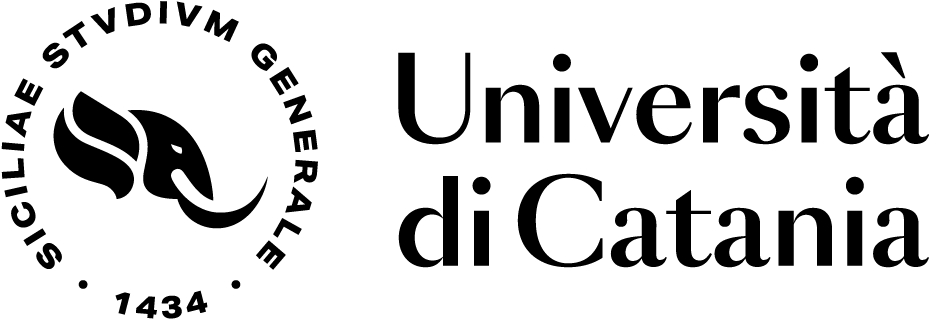
\includegraphics[width=0.85\textwidth]{immagini/foto_dfa/UniCT-Logo-Nero.png}
        \end{flushleft}
    \end{minipage}
            \hfill
    \begin{minipage}[c]{0.45\textwidth}
        \begin{flushright}
            
\includegraphics[width=\textwidth]{immagini/foto_dfa/logo_dfa_orizzontale.jpg}
        \end{flushright}
    \end{minipage}\\
    \medskip
    \scshape{\bfseries Corso di Laurea in Physics}
    \rule{\textwidth}{1pt}\\
    \vspace{4cm}
    %\normalfont\Large\thesisfont{Appunti di}\\
    \huge
    \thesisfont{Supeconductivity and Superfluidity}\\
    \medskip
    \rule{\textwidth}{1pt}\\
    \medskip
    \large
    \thesisfont{Corso tenuto dalla Prof.ssa~Paladino nell'A.A. 2024/2025}

    \vspace{2.5cm}

    %\large
    %\thesisfont{M. Agozzino, A. Biondo\\D. Di Prima, E. Di Stefano}
    
    \vspace{2.5cm}
    \normalsize


    \vfill
\end{center}
\end{titlepage}
    
\restoregeometry
%\thispagestyle{empty}
%%%%%%%           Indice
%% Toglie numero pagina al centro nelle pagine dispari di titolo, sia nel toc che in biblio e nell'indice analitico
\makeatletter
\let\ps@plain\ps@fancytitle\makeatother

\newgeometry{
    top=2.3cm,bottom=2.3cm,
    %% Margini
    left = 2.3cm,
    right=5.2cm,
    marginparsep=0cm,
    marginparwidth=4.3cm,
    %%% Contenuto
    %textwidth=14cm,
    %textheight=180mm,
    %headheight=21pt,
    %%%%%%5 Header e footer
    %headsep=10pt,
    %footskip=20pt,
    %footnotesep=10pt,
}
\tableofcontents
\restoregeometry
%\cleardoublepage




\mainmatter\thispagestyle{fancytitle}
\phantomsection
%\chapter*{Prefazione}
%\addcontentsline{toc}{chapter}{Prefazione}
% \clearpage

\thispagestyle{empty}

%\chapter{Introduzione}
%\input{Capitoli/0.Introduzione.tex}

\chapter{Effetti caratteristici e teorie fenomenologiche}
\section{Un quadro storico}
%\begin{figure}[H]
%   \centering
%   
\includegraphics[width=\textwidth]{Immagini/Tabella_scoperte.png}
%\end{figure}
\begin{table}[H]
   \centering
   \footnotesize
   \begin{tabular}{ll}
      \hline
      &\\[-0.2cm]
      1908 & Liquefazione di $^4$He a 4.2 K \\[0.1cm]
      1911 & Scoperta della superconduttività nel Hg a 4.1 K \\[0.1cm]
      1925 & Predizione della condensazione di Bose--Einstein (BEC) \\[0.1cm]
      1927 & Transizione $\lambda$ osservata in $^4$He a 2.2 K \\[0.1cm]
      1933 & Osservazione dell'effetto Meissner--Ochsenfeld \\[0.1cm]
      1938 & Dimostrazione della superfluidità in $^4$He \\[0.1cm]
      1950 & Teoria di Ginzburg--Landau della superconduttività \\[0.1cm]
      1957 & Teoria Bardeen--Cooper--Schrieffer (BCS) \\[0.1cm]
      1957 & Reticolo di flusso di Abrikosov \\[0.1cm]
      1962 & Effetto Josephson \\[0.1cm]
      1963--1964 & Meccanismo di Anderson--Higgs \\[0.1cm]
      1971 & Superfluidità osservata in $^3$He a 2.8 mK \\[0.1cm]
      1986 & Scoperta della superconduttività ad alta temperatura, 30--165 K \\[0.1cm]
      1995 & Realizzazione della BEC in gas atomici, 0.5 $\mu$K \\[0.1cm]
      \hline
   \end{tabular}
\end{table}
Nella tabella sopra possiamo vedere storicamente quando sono stati scoperti questi fenomeni e quali sono stati i principali passi nello sviluppo della teoria. Osserviamo che si tratta di un fenomeno relativamente recente, poiché le prime evidenze risalgono al 1908, e tutta la storia ha origine dalla liquefazione dell'$\rm ^4He$ a 4.2 K. Fondamentalmente, il motivo per cui questo fenomeno è stato scoperto così tardi è che si manifesta a temperature molto basse, quindi finché non è stato possibile raggiungere tali temperature, non è stato osservato.\\
Solo pochi anni dopo, la superconduttività fu scoperta nel mercurio, dove la transizione avviene a circa 4.1 K. All'epoca il fenomeno non era affatto compreso, fu semplicemente una sorpresa. Allo stesso tempo furono fatti anche alcuni sforzi sul lato teorico, e venne formulata la previsione della condensazione di Bose-Einstein. Dunque, mentre la superconduttività fu prima osservata e solo in seguito spiegata, per la condensazione di Bose-Einstein avvenne il contrario: prima venne prevista teoricamente e solo molto tempo dopo fu osservata sperimentalmente. Infatti, la condensazione di Bose-Einstein fu osservata circa 70 anni dopo.\\
La caratteristica della superconduttività che fu scoperta nel 1911 riguardava la perfetta conducibilità. Le proprietà magnetiche vennero osservate poco dopo, nel 1930, con l'effetto Meissner-Ochsenfeld, che è legato alla risposta di un superconduttore a un campo magnetico. Nel 1938 fu dimostrata la superfluidità dell'$\rm ^4He$. Le prime teorie sulla superconduttività e sulla superfluidità risalgono alla metà del XX secolo, con la teoria di Ginzburg--Landau, la teoria BCS e i contributi di Abrikosov e Josephson, fondamentali per comprendere diverse parti del fenomeno. Negli stessi anni fu scoperto anche il meccanismo di Anderson-Higgs. Quest'ultimo potrebbe sembrare un argomento totalmente scollegato da ciò di cui stiamo parlando, ma in realtà non lo è, e vedremo in che modo.\\
Nel 1971, la superfluidità fu scoperta anche nell'$\rm ^3He$ a 2,8 mK. Un'altra peculiarità della superfluidità è che esistono due tipi di superfluidità: il primo materiale in cui fu osservato questo comportamento fu l'$\rm ^4He$, poiché ha una temperatura di transizione alla superfluidità dell'ordine dei Kelvin, mentre nell'$\rm ^3He$ il fenomeno si manifesta a temperature molto più basse, dell'ordine dei mK, ed è stato quindi scoperto molto più tardi.\\
Negli anni '80 furono scoperti nuovi materiali in cui la superconduttività si verifica ad alte temperature, dove "alte temperature" significa tra 30 K e 150 K o anche di più. Infine, nel 1995 fu osservata la condensazione di Bose-Einstein nei gas atomici.\\
Da questa tabella possiamo vedere il grande sforzo che è stato compiuto per comprendere questi fenomeni, che sono stati scoperti e spiegati nell'arco di circa un secolo, con differenze fondamentali che analizzeremo.\\
La caratteristica comune a questi tre fenomeni, la condensazione di Bose-Einstein, la superfluidità e la superconduttività, è che rappresentano stati quantistici macroscopici della materia. Sono quindi fenomeni quantistici e macroscopici, ma con proprietà totalmente differenti. La caratteristica fondamentale che li distingue è che la condensazione di Bose-Einstein si verifica in sistemi bosonici, composti da bosoni non interagenti, quindi non è un fenomeno che richiede interazione tra particelle. Al contrario, la superfluidità e la superconduttività dipendono dall'interazione tra particelle. Tuttavia, i superconduttori sono sistemi fermionici e interagenti, ed è questa la loro particolarità, mentre la superfluidità può manifestarsi sia con proprietà bosoniche che con proprietà fermioniche: questa è la principale differenza tra l'Elio-4 e l'Elio-3. Entrambi i casi, però, richiedono una qualche forma di interazione tra le particelle. Durante il corso vedremo in che modo questi elementi entrano in gioco e quali sono le differenze tra i vari meccanismi.
%In this table we can see how historically this phenomenon was discovered and which were the main steps of the theory. Ew see it's a phenomenon which is relatively new, because the first evidence came back to the 1908, and the whole story comes from the liquefation of $\rm ^4He$ at 4.2 Kelvin and basically the reason why this phenomenon was discovered relatively late is the fact that they take place at very low temperatures, so until it was not impossible to reach this low temperature, they were not observed. Just a few years later superconductivity was discovered in Mercury where the transition takes place at about 4.1, Kelvin. The phenomenon was not understood at all at that time, it was just a surprise, and now we're going to see which were those observations but at the same time there were some efforts also on the theory side, and there was the prediction of the Bose-Einstein condensation. So while superconductivity was first observed and then later explained, for Bose-Einstein condensation it was the other way around, it was first predicted and only much later observed. You see that the Bose-Einstein condensation is observed in about 19 years later. In 1911 the feature of superconductivity, which was discovered, was the perfect conductivity. The magnetic properties were observed shortly after, in 1930, with the Meissner-Ochsenfled effect, which is related to the response of a superconductor to a magnetic field. In 1938 there was the demonstration of superfluidity in $\rm ^4He$. The first theories on superconductivity and superfluidity come around the mid-1990s with the Ginzburg--Landau theory, the BCS theory, and Abrikosov and Josephson giving relevant in the contribution to understand different parts of the phenomenon. In the same years, also the Anderson-Hicks mechanism was discovered. It might seem totally disconnected by what we are saying here, but actually it is not, and we are going to see in which respect. In 1971, superfluidity was found in $\rm ^3He$ at 2.8 mK, so another peculiarity of superfluidity is that we are two types of superfluidity, and the material which was observed to have a superfluid behavior first was $\rm ^4He$, because it has a superfluid transition temperature, which is of the order of Kelvin, whereas in $\rm ^3He$ it takes place at mK, so it was discovered much later. And in around the 80s, also new materials were discovered, where superconductivity takes place at high temperatures, so high temperatures means between 30 K and 150 K or even more. Finally, in 1995, it was observed Bose-Einstein condensation in atomic gases. We see from this table that there was a great effort towards this phenomena, that this phenomena were discovered and understood in about one century, with critical differences which we are going to see among all of them. The key word, which is common to these three phenomena, Bose-Einstein condensation, superfluidity and superconductivity, is that they all represent macroscopic quantum states of matter. So they are quantum and they are macroscopic, but with totally different properties, and the key properties which make them different are that Bose-Einstein condensation takes place in bosonic systems, which are bosons, and they are not interacting, so it's not a phenomenon which requires an interaction. Whereas this is the case for superfluids and superconductors, but superconductors are fermionic systems and interacting, and so these are the two characteristics. Superfluids can be either with bosonic properties or with fermionic properties, and this is the main difference between Helium-4 and Helium-3, and they require some sort of interaction with the particles. So these are the main differences, and we are going to see during this course how these elements come into play, and which is the difference between the mechanisms.
\section{Superconduttività}
%We start with superconductivity, and the basic phenomena of superconductivity are electromagnetic properties and thermodynamic properties. Electromagnetic properties are the perfect conductivity and the perfect diamagnetism, whereas the thermodynamic properties are described by a peculiar electronic specific heat, which differs from the specific heat we have in normal metals under some conditions.
%\subsection{Conducibilità perfetta}
%Let's start from the most popular property of superconductors, the perfect conductivity. It was observed in 1911 by Holmes. He was measuring the resistance of mercury by varying temperature and, unexpectedly, he observed that by decreasing temperature, at the temperature of 4.2 K the resistance was reduced abruptly of about 5 order of magnitudes so becoming almost vanishing for temperatures below this temperature. This was clearly a surprise: there was no reason why the material apparently should have become totally conductive (and the the name superconductor comes precisely from this observation so it's perfect conductor, provided temperature is sufficient small) And this vanishing superconductivity is detected for instance nowadays if one performs experiments with rings of superconductive material and what is observed is that once the supercurrent is setted in, the supercurrent stays without any variation and the variations are detected by measuring the magnetic field which is created by the supercurrent flowing in the ring with NMR methods because they allow detecting even very tiny variation of the magnetic field. So, from considering the basically vanishing variation of the magnetic field over some finite time in the surface of the ring, one can extrapolate that the supercurrent would flow forever basically without any dissipation. 
Iniziamo con la superconduttività, i cui fenomeni fondamentali riguardano le proprietà elettromagnetiche e termodinamiche. Le proprietà elettromagnetiche includono la perfetta conducibilità e il perfetto diamagnetismo, mentre le proprietà termodinamiche sono descritte da un peculiare calore specifico elettronico, che differisce dal calore specifico che si osserva nei metalli normali in determinate condizioni.
\subsection{Conducibilità perfetta}
Iniziamo dalla proprietà più nota dei superconduttori: la conducibilità perfetta. Essa fu osservata per la prima volta nel 1911 da Holmes. Durante la misurazione della resistenza del mercurio al variare della temperatura, osservò inaspettatamente che, abbassando la temperatura, a 4.2 K la resistenza diminuiva bruscamente di circa cinque ordini di grandezza, diventando praticamente nulla per temperature inferiori a questo valore.\\
\begin{marginfigure}
   \centering
   
\includegraphics[width=.8\textwidth]{Immagini/Grafico_Holmes.png}
   \caption*{Resistenza del mercurio in funzione della temperatura.}
\end{marginfigure}
\hspace{-0.165cm}Questa scoperta fu una sorpresa: non c'era alcuna ragione apparente per cui il materiale dovesse diventare totalmente conduttivo (ed è proprio da questa osservazione che deriva il nome "superconduttore", ovvero un conduttore perfetto, a condizione che la temperatura sia sufficientemente bassa).\\
Oggi questa assenza di resistenza viene rilevata, ad esempio, in esperimenti con anelli di materiale superconduttore. In questi esperimenti si osserva che, una volta avviata una corrente di supercorrente, essa rimane invariata nel tempo. Le variazioni della supercorrente vengono misurate attraverso il campo magnetico generato dalla corrente che scorre nell'anello, utilizzando metodi NMR (Risonanza Magnetica Nucleare), che consentono di rilevare anche variazioni minime del campo magnetico. Dall'osservazione della variazione praticamente nulla del campo magnetico in un intervallo di tempo finito sulla superficie dell'anello, si può dedurre che la supercorrente potrebbe fluire indefinitamente senza alcuna dissipazione.\\
%Holmes observed this phenomenon, the perfect conductivity, in the absence of a magnetic field. In general, if there is a magnetic field, this phenomenon takes place provided this magnetic field is not wide. So, up to what is called the critical magnetic field $H_c(T)$, if the system feels a magnetic field higher than this critical value, even if we decrease the temperature going below this critical temperature, we do not observe the superconducting behavior, so vanishing resistance.
Holmes osservò questo fenomeno, la perfetta conducibilità, in assenza di un campo magnetico. In generale, se è presente un campo magnetico, questo fenomeno si verifica a condizione che il campo non sia troppo intenso. Infatti, fino a un valore detto \emph{campo magnetico critico} $H_c(T)$, il materiale rimane superconduttore. Tuttavia, se il sistema è esposto a un campo magnetico superiore a questo valore critico, anche abbassando la temperatura al di sotto della temperatura critica non si osserva il comportamento superconduttivo, ovvero la resistenza non si annulla.
\subsection{Diamagnetismo perfetto}
Un'altra proprietà fondamentale dei superconduttori, scoperta alcuni anni dopo, è il diamagnetismo perfetto, noto anche come \emph{effetto Meissner}. Tale fenomeno è illustrato schematicamente nella figura seguente.
\begin{figure}[H]
   \centering
   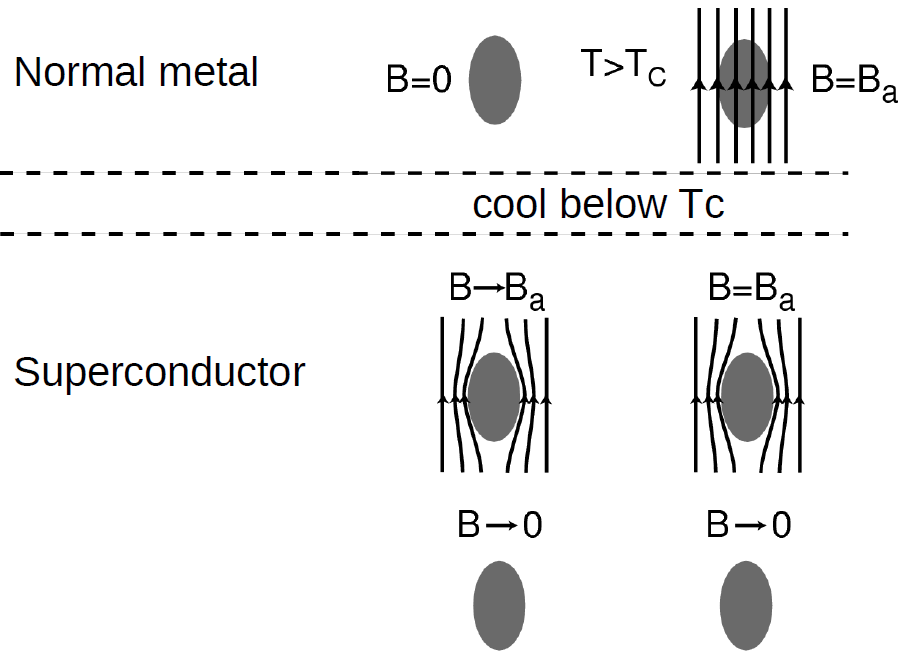
\includegraphics[width=0.8\textwidth]{immagini/Effetto_Meissner_1.png}
\end{figure}
\hspace{-0.6cm}Supponiamo che l'oggetto grigio rappresenti un materiale in grado di diventare superconduttore. Esso può trovarsi sia in assenza sia in presenza di un campo magnetico esterno.\\ Consideriamo ora la possibilità di raffreddare il sistema al di sotto della cosiddetta temperatura critica $T_c$, ossia la temperatura al di sotto della quale emerge il comportamento superconduttivo. Se inizialmente il materiale si trova a una temperatura $T > T_c$ e non è presente alcun campo magnetico, esso si comporta come un metallo normale. Raffreddando il sistema al di sotto di $T_c$, il materiale diventa superconduttore. Se a questo punto si applica un campo magnetico esterno, tale campo non riesce a penetrare all'interno del campione. Se successivamente il campo magnetico viene rimosso, all'interno del materiale non rimane alcun campo magnetico.\\
Consideriamo ora il caso opposto, in cui il materiale si trovi inizialmente nello stato normale ma in presenza di un campo magnetico applicato. In questa situazione il campo magnetico penetra all'interno del metallo, come avviene tipicamente nei conduttori normali. Tuttavia, se il materiale viene raffreddato al di sotto della temperatura critica, il campo magnetico viene espulso dal suo interno. Se successivamente il campo magnetico esterno viene spento, il sistema rimane privo di campo magnetico interno.\\
Osserviamo quindi che, indipendentemente dalle condizioni iniziali, una volta che il sistema si trova nello stato superconduttivo, cioè al di sotto della temperatura critica, il campo magnetico all'interno del materiale risulta nullo.\\
A questo punto sorge una domanda: se inizialmente abbiamo un metallo normale immerso in un campo magnetico, come è possibile che, raffreddandolo al di sotto della temperatura critica senza modificare il campo applicato, il campo magnetico all'interno del materiale diventi nullo? Questo implica che il campo magnetico totale all'interno del materiale debba essere compensato da un'altra sorgente di campo magnetico.\\
La spiegazione è la seguente. Se un materiale entra nello stato superconduttivo in presenza di un campo magnetico esterno, al momento della transizione di fase si genera una supercorrente che scorre sulla superficie del campione. Tale supercorrente produce un campo magnetico che si oppone al campo applicato e lo compensa esattamente all'interno del materiale.\\
Questo comportamento è detto diamagnetismo. Utilizzando infatti la relazione che lega il campo di induzione magnetica $\vb{B}$ al campo magnetico $\vb{H}$ e alla magnetizzazione $\vb{M}$,
\begin{equation*}
   \vb{B} = \vb{H} + 4\pi \vb{M}
\end{equation*}
si vede che, nello stato superconduttivo, la condizione $\vb{B}=0$ all'interno del materiale implica una magnetizzazione pari a
\begin{equation*}
   \vb{M} = -\frac{\vb{H}}{4\pi}
\end{equation*}
Questa relazione descrive il cosiddetto diamagnetismo perfetto, che rappresenta una delle proprietà caratteristiche dello stato superconduttivo.\\
Tipicamente, in un materiale diamagnetico, la magnetizzazione è opposta al campo magnetico esterno, ma con una suscettibilità inferiore. In questo caso, invece, si ha un comportamento diamagnetico perfetto, ed è per questo motivo che l'espulsione del campo magnetico da un superconduttore è chiamata anche effetto diamagnetico.\\
L'effetto di espulsione del campo magnetico da un superconduttore avviene solo se il campo magnetico applicato è sufficientemente piccolo. Quindi, non si verifica per qualsiasi campo magnetico applicato, ma solo se quest'ultimo è inferiore a un valore detto campo critico $H_c$. Questo campo critico dipende dalla temperatura, per cui $H_c \equiv H_c(T)$. La dipendenza del campo critico $H_c$ dalla temperatura, per molti materiali, è descritta da una legge di potenza della forma:  
\begin{equation}
   H_c(T)
   =H_c(0) \biggl[ 1 - \qty( \frac{T}{T_c} )^2 \biggr]
   \label{eq:campo_critico}
\end{equation}
dove $H_c(0)$ è il valore estrapolato del campo critico allo zero assoluto.
\begin{figure}[H]
   \centering
   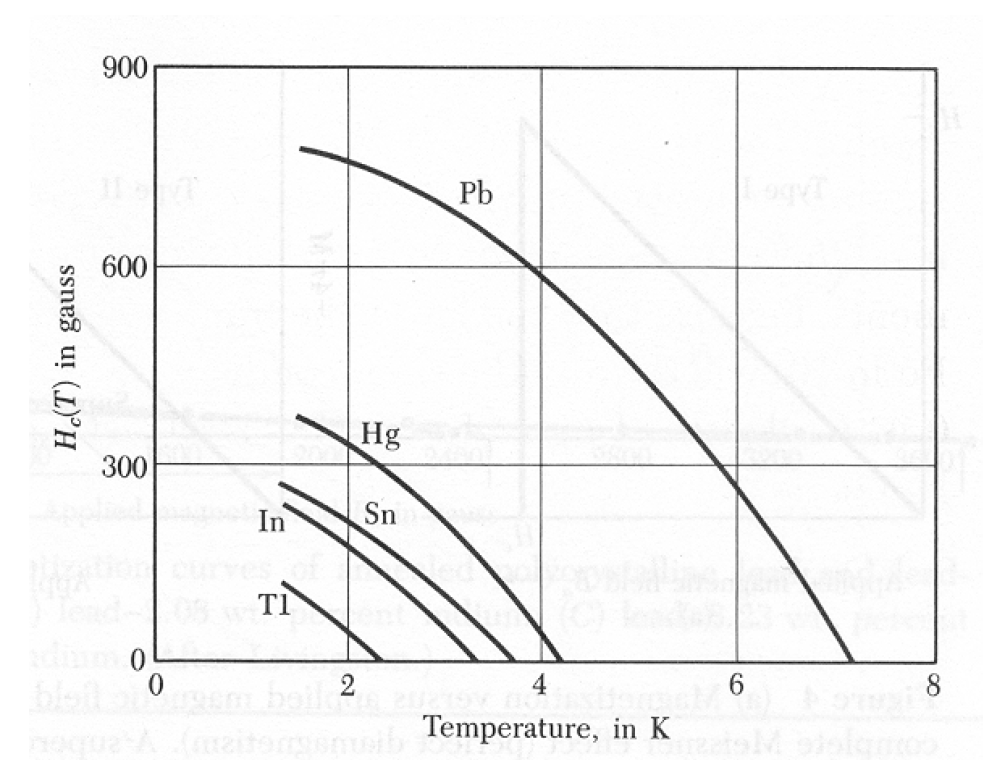
\includegraphics[width=.6\textwidth]{immagini/curve_campo_magnetico_temperatura_superconduttori.png}
   \caption*{Campo magnetico critico in funzione della temperatura per diversi materiali.}
\end{figure}
\hspace{-0.6cm}L'\eqrefcustom{eq:campo_critico} è una legge empirica. Inoltre, se sull'asse orizzontale si riporta la temperatura assoluta normalizzata rispetto alla temperatura critica, mentre sull'asse verticale si rappresenta il valore del campo magnetico esterno applicato fino al quale si osserva la superconduttività (o, equivalentemente, al di sotto del quale il materiale è superconduttivo), scalato rispetto al valore estrapolato del campo critico, tutte le curve si sovrappongono in un'unica linea che descrive accuratamente il comportamento di questa classe di materiali:
\begin{figure}[H]
   \centering
   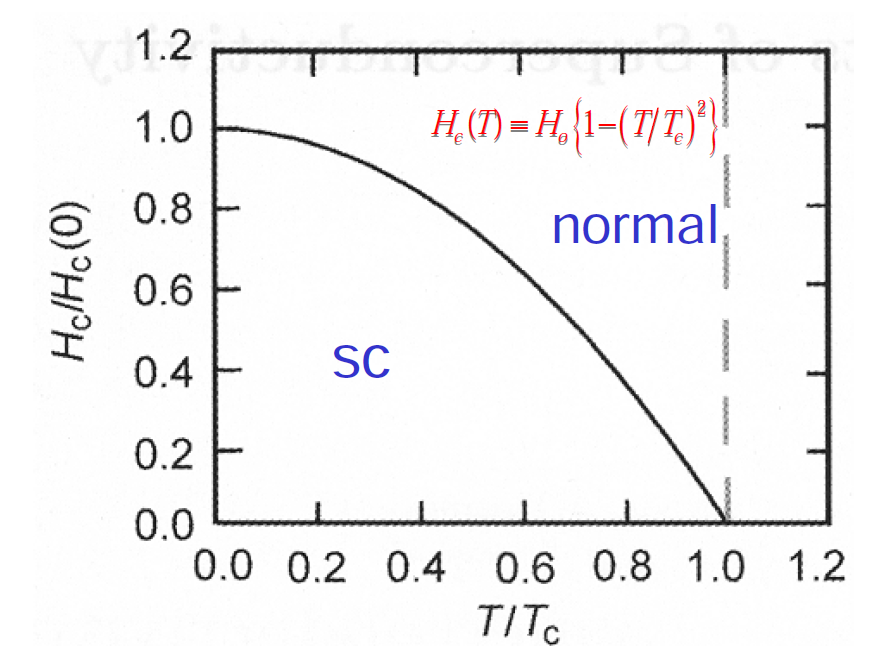
\includegraphics[width=.6\textwidth]{immagini/curve_campo_magnetico_temperatura_superconduttori_riscalate.png}
\end{figure}
\hspace{-0.6cm}Ciò che questa sorta di diagramma di fase ci dice è che nella regione dei campi magnetici inferiori a $H_c$ e delle temperature inferiori alla temperatura critica, il materiale è superconduttore. Al di sopra di questa curva, invece, il materiale si comporta come un metallo normale. Inoltre, la curva si annulla alla temperatura critica, il che significa che, per temperature superiori alla temperatura critica, indipendentemente dal valore del campo magnetico, la superconduttività non è presente.\\
Cerchiamo adesso di capire se queste due proprietà, il fatto che il materiale diventi un conduttore perfetto e il fatto che si verifichi l'espulsione del campo magnetico, rappresentino due fenomeni indipendenti oppure se una possa essere derivato dall'altro.\\
La risposta è che si tratta di due fenomeni indipendenti. Per capirne il motivo, supponiamo che un superconduttore sia semplicemente un conduttore perfetto (ossia supponiamo che il materiale abbia resistenza nulla in determinate condizioni, che è ciò che intendiamo con questa definizione) e cerchiamo di capire quale sarebbe la sua risposta a un campo magnetico applicato. Confrontiamo poi questa risposta con quella effettivamente osservata in un superconduttore.\\
Supponiamo quindi di avere un conduttore perfetto, descritto come un materiale con resistività nulla. Dalla legge di Ohm sappiamo che il campo elettrico è dato da:
\begin{equation*}
   \vb{E}=\rho\vb{J}
\end{equation*}
Dunque, se la resistività $\rho$ è zero, significa che in un conduttore perfetto il campo elettrico è nullo, anche in presenza di una corrente non nulla.\\
Se ora utilizziamo la legge di Faraday, sappiamo che il rotore del campo elettrico è legato alla derivata temporale del campo magnetico da:
\begin{equation*}
   \curl{\vb{E}}=-\frac{1}{c} \pdv{\vb{B}}{t}
\end{equation*}
Dato che in un conduttore perfetto il campo elettrico è nullo, ciò implica che il campo magnetico deve rimanere costante nel tempo. Quindi per un conduttore perfetto ci aspettiamo che possano esserci correnti non nulle, resistività nulla, ma che il campo magnetico rimanga costante nel tempo.\\
Proviamo ora a prevedere cosa osserveremmo in un conduttore perfetto considerando due situazioni:
\begin{enumerate}[leftmargin=0.7cm, label=(\alph*)]
   \item Un conduttore perfetto in assenza di campo magnetico, che viene raffreddato sotto la temperatura critica.
   \item Un conduttore perfetto in presenza di un campo magnetico applicato, che viene raffreddato sotto la temperatura critica.
\end{enumerate}
Confronteremo poi queste previsioni con il comportamento reale di un superconduttore.
\begin{figure}[H]
   \centering
   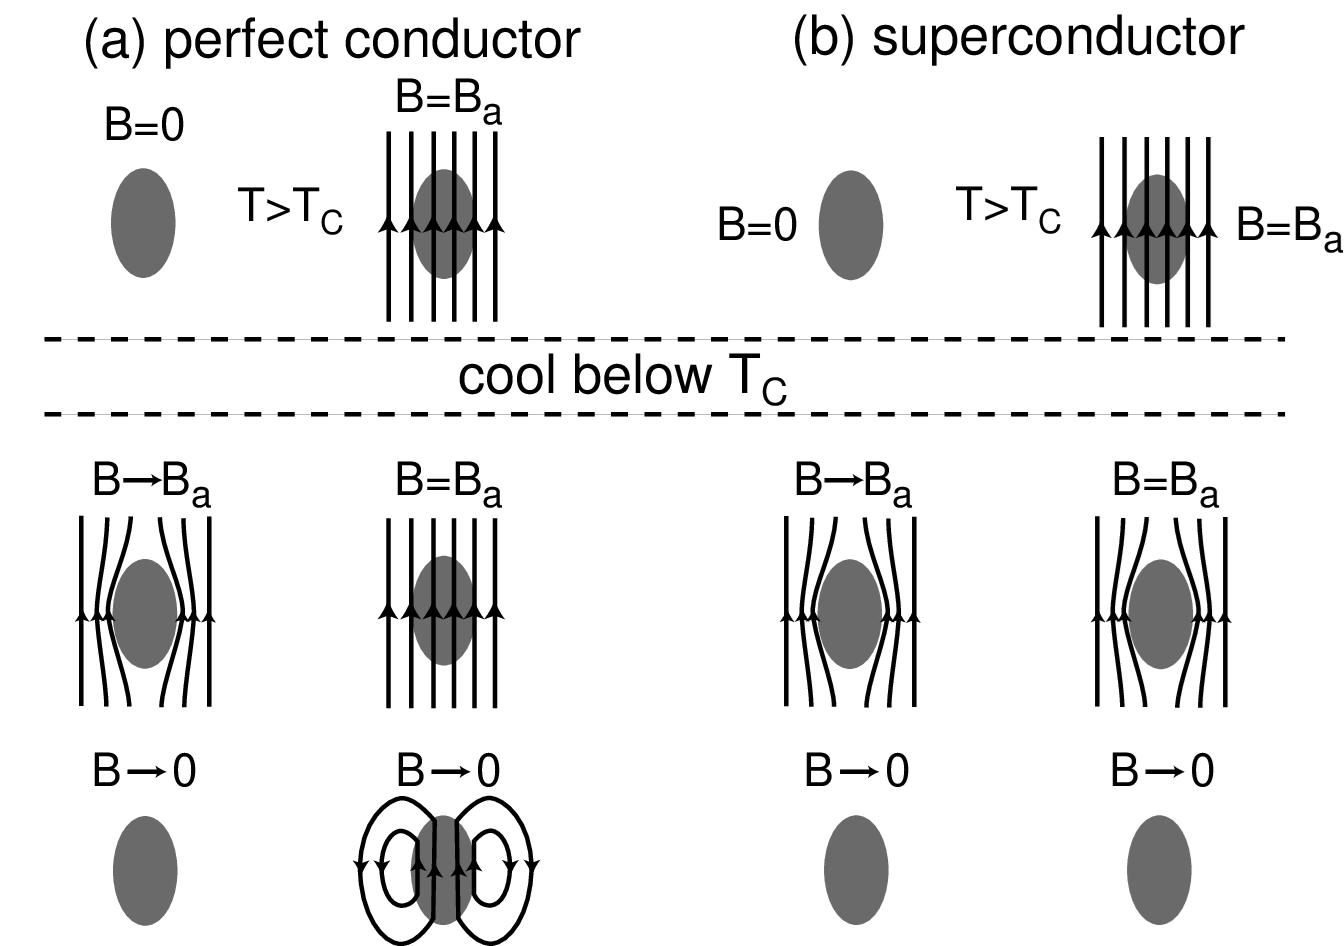
\includegraphics[width=.9\textwidth]{immagini/confronto_conduttori_perfetti_superconduttori.png}
\end{figure}
\hspace{-0.6cm}Iniziamo dall'esperimento sulla sinistra. Se inizialmente non abbiamo un campo magnetico applicato, ci aspettiamo che raffreddando il materiale, poiché $\vb{B}$ deve rimanere costante, dato che inizialmente era nullo all'interno del materiale esso sarà ancora pari a zero anche quando il materiale sarà diventato superconduttore e resterebbe nullo anche se accendessimo e poi spegnessimo un campo magnetico. Questo tipo di comportamento sarebbe perfettamente spiegato dalla teoria del conduttore perfetto.\\
Vediamo ora cosa accade se invece consideriamo un conduttore perfetto in presenza di un campo magnetico applicato. All'inizio, essendo un metallo normale, il campo magnetico penetra nel materiale. Supponiamo ora di raffreddarlo: se il materiale è un conduttore perfetto, la legge di Faraday ci dice che $\vb{B}$ dovrebbe rimanere costante nel tempo, quindi il campo magnetico dovrebbe rimanere all'interno del materiale. Anche se spegniamo il campo esterno, il campo magnetico dovrebbe persistere all'interno del conduttore perfetto. Tuttavia, questo non è ciò che si osserva in un superconduttore, in quanto quando un materiale diventa superconduttore in presenza di un campo magnetico applicato il campo viene espulso dal materiale. Se confrontiamo i due casi, conduttore perfetto in presenza di un campo magnetico e superconduttore in presenza di un campo magnetico, vediamo una differenza fondamentale.\\
Tale fatto ci dice che la conducibilità perfetta (cioè resistività nulla) non è sufficiente per spiegare il comportamento osservato nei superconduttori quando il campo magnetico iniziale è diverso da zero. In particolare, l'effetto Meissner non può essere spiegato solo con la perfetta conducibilità. Queste considerazioni ci portano a concludere che la perfetta conducibilità e il perfetto diamagnetismo sono due fenomeni indipendenti.
%Let's start from the left experiment, We have zero applied magnetic field, we cool down the material then what we have to expect in this case that B is constant so zero initially zero when there is an applied magnetic field even below the critical temperature and still zero if we turn off the field. This type of experiment would be perfectly explained for a perfect conductor.\\
%Let's see what happens if instead we describe what we would expect for a perfect conductor if initially there is an applied magnetic field. So in a perfect conductor in an applied magnetic field, since it's a normal metal, there is an applied field that penetrates the conductor. Now let's suppose we cool it down but if we cool it down since $\vb{B}$ should stay constant we have to expect that the magnetic field still persists inside the material and if we switch off the applied magnetic field still this magnetic field should exist inside the perfect conductor. So for a perfect conductor in an applied magnetic field even if we force it to undergo a transition below the critical temperature we should expect that the magnetic field still remains inside the material. But this is not what we observe for a superconductor because what we observe for a superconductor in the presence of an applied magnetic field when we induce the transition in the presence of an applied magnetic field is the expulsion of the magnetic field out of the material. So if we compare these two left, these two columns, this one what happens in an applied magnetic field for a perfect conductor and what happens in an applied magnetic field for a superconductor we see a difference. This tells us that perfect conductivity, meaning zero resistivity, cannot explain what happens to a superconductor when the magnetic field is different from zero initially, whereas it would explain what happens if there is no applied magnetic field. So the peculiar Meissner effect which is the expulsion of the magnetic field out of the sample cannot be explained by the perfect conductivity. So this tells us that these two phenomena, perfect conductivity and perfect diamagnetism, are two independent phenomena. In summary, perfect conductivity cannot explain the Meissner effect.
\subsection{Termodinamica della transizione N--SC}
%Let's try to rephrase what we have observed. The superconductor is characterized by the condition $B=0$ inside it independently on how the system has reached this condition, so there is zero magnetic field inside if there was not inside at the beginning then the magnetic field was turned on and then it is turned off and there is zero magnetic field inside even if we initially had the magnetic field inside. In other words, in the superconducting phase we have the same state with zero magnetic field inside independently on how the system has reached this condition. This means that the superconducting phase is a thermodynamically stable phase of the material, and this leads us to describe it in thermodynamic terms. In particular, ew can describe the two conditions of the material, which is either normal or superconducting, as different phases of matter which we have to describe in terms of appropriate thermodynamic potential.
Proviamo a riformulare ciò che abbiamo osservato. Il superconduttore è caratterizzato dalla condizione $\vb{B}=0$ al suo interno, indipendentemente da come il sistema abbia raggiunto questa condizione. Ciò significa che il campo magnetico all'interno è nullo sia nel caso in cui inizialmente non fosse presente, poi acceso e successivamente spento, sia nel caso in cui inizialmente fosse presente. In altre parole, nella fase superconduttiva si ha sempre lo stesso stato con campo magnetico nullo all'interno, indipendentemente dal modo in cui il sistema ha raggiunto questa condizione. Questo implica che la fase superconduttiva è una fase termodinamicamente stabile del materiale, il che ci porta a descriverla in termini termodinamici. In particolare, possiamo descrivere le due condizioni del materiale, ovvero lo stato normale e quello superconduttivo, come fasi distinte della materia, che dobbiamo rappresentare attraverso un opportuno potenziale termodinamico.\\
%The idea is that the system reaches the thermodynamic stable state following the second law of thermodynamics, provided we use the appropriate thermodynamic potential. Describing a system using the appropriate thermodynamic potential means identifying the thermodynamic potential which stays constant at the transition, where the transition takes place in particular changing the temperature and changing the applied magnetic field, so we have to find the appropriate thermodynamic potential which is stable at the transition when the two variables which change, we modify, are magnetic field and temperature. Then let's make a step in between and remind which are the thermodynamic relations in the presence of a magnetic field in general and this will lead us to identify which is the appropriate thermodynamic potential to describe the superconductive transition. First of all we have to identify what is the system. The system is a magnetized sample of the material of fixed volume $V$ and magnetic field. Let's write the two most common free energies for this system, which are the Helmholtz free energy and the Gibbs free energy and now we are going to see how to write these two free energies.
L'idea è che il sistema raggiunga lo stato termodinamicamente stabile seguendo la seconda legge della termodinamica\mn{Tale principio afferma che "Per un sistema chiuso, l'entropia $S$ aumenta, mentre $U$, $H$, $F$ e $G$ diminuiscono, nei limiti consentiti dalla termodinamica. Ciò permette di formulare affermazioni sulla stabilità degli stati di equilibrio termodinamico.".}, a condizione che si utilizzi il potenziale termodinamico appropriato. Descrivere un sistema attraverso il potenziale termodinamico appropriato significa identificare il potenziale termodinamico che rimane costante durante la transizione, la quale avviene in particolare al variare della temperatura e del campo magnetico applicato. Dobbiamo quindi trovare il potenziale termodinamico adeguato, che sia stabile durante la transizione quando le due variabili che modifichiamo, ovvero il campo magnetico e la temperatura, cambiano.\\
Facciamo ora un passo intermedio e ricordiamo quali sono le relazioni termodinamiche in presenza di un campo magnetico in generale: questo ci porterà a identificare il potenziale termodinamico più adatto a descrivere la transizione superconduttiva. Per prima cosa, dobbiamo identificare il sistema. Il sistema è un campione magnetizzato del materiale di volume fissato $V$ e con campo magnetico definito. Scriviamo quindi le due energie libere più comuni per questo sistema, ovvero l'energia libera di Helmholtz e l'energia libera di Gibbs, e vediamo ora come esprimerle:
\begin{itemize}[leftmargin=0.5cm]
   \item L'energia libera di Helmholtz $F$ è definita come:
   \begin{equation*}
      F=E - TS
   \end{equation*}
   dove $E$ è l'energia interna del sistema e $S$ è l'entropia. Se facciamo una variazione infinitesima di queste quantità, avremo una variazione infinitesima dell'energia libera, data da:
   \begin{equation*}
      \dd{F}
      =\dd{E} - \dd{(TS)}
      =\dd{E} - T\dd{S} - S\dd{T}
   \end{equation*}
   Dalla prima legge della termodinamica sappiamo che $\dd{E}=\var{Q} - \dd{W}$, dove $-\dd{W}$ è il lavoro magnetico svolto sul sistema per stabilire il campo nel volume $V$ e magnetizzare il campione. Inoltre, in una trasformazione quasi-statica e reversibile, il calore scambiato si scrive come: $\var{Q}=T\dd{S}$, per cui possiamo scrivere
   \begin{equation*}
      \dd{F}
      =( T\dd{S} - \dd{W} ) - T\dd{S} - S\dd{T}
      =- \dd{W} - S\dd{T}
   \end{equation*}
   Il lavoro magnetico può essere espresso in termini del differenziale dell'energia del campo magnetico:
\begin{equation*}
   \dd{W}
   =\dd{ \qty( \frac{V H^2}{8\pi} ) } + V H \dd{M}
\end{equation*}
dove il primo termine è dato dal prodotto del volume del materiale moltiplicato per la densità di energia del campo magnetico e il secondo termine è l'energia necessaria per magnetizzare il campione. Poiché $V$ è costante, possiamo scrivere:
\begin{equation*}
   \dd{ \qty( \frac{V H^2}{8\pi} ) }
   =\frac{V H}{4\pi} \dd{H}
\end{equation*}
e quindi, ricordando che $B=H + 4\pi M$, otteniamo:
\begin{equation*}
   \dd{W}
   =\frac{V H}{4\pi} ( \dd{H} + 4\pi \dd{M} )
   =\frac{V}{4\pi} H \dd{B}
\end{equation*}
Di conseguenza, la variazione dell'energia libera di Helmholtz è data da
\begin{equation*}
   \dd{F(T,B)}
   =- \frac{V}{4\pi} H \dd{B} - S \dd{T}
\end{equation*}
Dall'espressione della variazione infinitesima dell'energia libera di Helmholtz, vediamo che esso è il potenziale termodinamico appropriato quando consideriamo una transizione che implica una temperatura $T$ e un'induzione magnetica $B$ costanti.
\item Se invece consideriamo l'energia libera di Gibbs, che per un sistema magnetico è definita come
\begin{equation}
   G(T,H)=F(T,B) - \frac{V}{4\pi} H B
   \label{eq:relazione_G_F}
\end{equation}
e ne facciamo una variazione infinitesima, otteniamo\mn{Nel caso più generale si ha che
\begin{equation*}
   \dd{(HB)}=\dd{H}B + H\dd{B}
\end{equation*}
ma essendo in questo caso $H$ costante, si ha che $\dd{(HB)}=H\dd{B}$.}:
\begin{equation*}
   \dd{G(T,H)}
   = - S \dd{T} - \frac{V}{4\pi} B \dd{H}
\end{equation*}
Ciò significa che $G$ è il potenziale termodinamico appropriato per una transizione che avviene a temperatura e campo magnetico $H$ fissati. Infatti, come abbiamo detto, quando avviene la transizione superconduttiva, il campo magnetico $\vb{B}$ viene espulso dal superconduttore. Questo significa che, per descrivere termodinamicamente la fase superconduttiva, non abbiamo bisogno di un potenziale termodinamico che dipenda dalle variazioni di $B$, ma piuttosto di un potenziale termodinamico che sia legato alle variazioni del campo magnetico esterno applicato, $H$. Questo $H$ viene mantenuto costante, poiché generalmente rappresenta il campo prodotto da una sorgente esterna, e non il campo magnetico presente nel campione.
\end{itemize}
%In fact, as we said when the superconductor transition takes place the magnetic field $\vb{B}$ is expelled from the superconductor, so it means that in order to describe thermodynamically the superconducting phase we do not need a thermodynamic potential which depends on variations of $B$ but we need a thermodynamic potential which is related to variations of the externally applied magnetic field $H$. This $H$ we keep constant because typically it is the field which comes from an externally applied field and not the magnetic field present in the sample.
Cerchiamo adesso di avvicinarci un po' di più a ciò che accade durante la transizione dalla fase normale alla fase superconduttiva in una geometria molto semplice. Supponiamo di avere un metallo di forma cilindrica di raggio $r_0$ e lunghezza $L$ posto all'interno di un solenoide di raggio $R$, lunghezza $L$ e avente $N$ spire.
\begin{figure}[H]
   \centering
   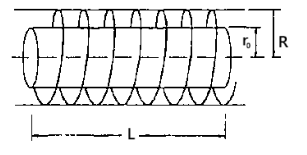
\includegraphics[width=.65\textwidth]{immagini/Cilindro_superconduttore.png}
\end{figure}
\hspace{-0.6cm}Partiamo dall'energia libera di Helmholtz e scriviamola per le due fasi, normale e superconduttiva. Nella fase normale abbiamo:
\begin{equation*}
   F_n=
   V f_{n,0} + V \frac{H_a^2}{8\pi} + V_{\text{ext}} \frac{H_a^2}{8\pi}
\end{equation*}
dove il primo termine rappresenta il contributo dell'energia libera di Helmholtz per unità di volume del campione nella fase normale in assenza di campo magnetico applicato, indicato con $f_{n,0}$, moltiplicato per il volume $V$ del materiale,\sn{Tale contributo è intrinseco alla fase normale del materiale e avrà un'espressione analoga quando il materiale sarà superconduttore.} mentre gli altri due termini rappresentano i contributi, se $H_a$ è il campo magnetico applicato proveniente dalla corrente che scorre nel solenoide, dovuti alla presenza di un campo magnetico all'interno del materiale e alla presenza di un campo magnetico nella parte del volume che si trova all'interno del solenoide, ma esterna al materiale (quindi $V_{\rm ext}$ rappresenta essenzialmente il volume di questa regione).\\  
%Now let's try to go a bit closer to what happens in the transition from the normal phase to the superconducting phase in a very simple geometry. Let's suppose we have a metal with a cylindrical shape and it is inside a solenoid of $N$ coils. Let's start from the Helmholtz free energy and we write it for the two phases, normal and superconducting. So in the normal phase we have where the first term is the contribution of the Helmholtz free energy per unit volume of the sample in the normal phase at zero applied magnetic field $f_n$ times the volume $V$ of the material\mn{Notice that this contribution is something which is intrinsic of the normal phase of the material. We will have the analogous expression when the material is superconducting}, and the other two terms are the contributions, if $H_a$ is the applied magnetic field coming from the current flowing in the solenoid, related to having a magnetic field inside the material plus the magnetic field in the part of the volume which is inside the solenoid, but external to the material (so $V_{\rm ext}$ is basically the volume of the region outside the material).\\
Nella fase superconduttiva, poiché abbiamo detto che non c'è campo magnetico applicato all'interno, non abbiamo il secondo contributo e quindi l'energia libera di Helmholtz è data da
\begin{equation*}
   F_s=
   V f_{s,0} + V_{\text{ext}} \frac{H_a^2}{8\pi}
\end{equation*}
Consideriamo adesso la differenza tra le due energie:
\begin{equation}
   F_n - F_s
   =V ( f_{n,0} - f_{s,0} ) + V \frac{H_a^2}{8\pi}
   \label{eq:differenza_energie_libere}
\end{equation}
\mn{Questa parte è da sistemare, chiedere ad Adriano o alla prof.}Supponiamo che il materiale sia inizialmente nella fase normale e che poi la temperatura venga modificata fino a farlo diventare superconduttore, mantenendo fissa la corrente nel solenoide (in quanto supponiamo che esso sia collegato ad un generatore) e quindi il campo magnetico applicato. In questo caso, poiché all'interno del materiale si verifica un cambiamento del campo magnetico (in quanto il campo viene espulso dal superconduttore), ci sarà una variazione del flusso del campo magnetico attraverso qualsiasi superficie avente come contorno il solenoide. Questo implica, per la legge di Faraday, che esiste un'energia associata a questo processo, data da:
%Suppose that this material is initially in the normal phase and then we change the temperature until it becomes superconducting while keeping fixed the current in the solenoid and so the magnetic field. Then, since what happens inside the material is a change of the magnetic field (because the magnetic field is expelled inside the material) we will have a variation of the flux of the magnetic field through any surface which has a solenoid as a contour. This implies, from the Faraday's law, that there is an energy related to this process which is given by
\begin{equation*}
   \dd{W}=\mathcal{E} I \dd{t}
\end{equation*}
dove $\mathcal{E}$ è la forza elettromotrice indotta e $I$ è la corrente che scorre nel solenoide. Se il processo avviene per un tempo finito, l'energia totale sarà data dall'integrale:
\begin{equation*}
   W=\int_{0}^{T} \mathcal{E} I \dd{t}
\end{equation*}
Dalla legge di Faraday sappiamo che $\mathcal{E}$ è data da
\begin{equation*}
   \mathcal{E}
   =-\frac{N}{c} \dv{\Phi}{t}
\end{equation*}
e sostituendo nell'integrale otteniamo\mn{Il flusso attraverso la superficie di una spira nella fase normale è dato da
\begin{equation*}
   \Phi_n=H_a \pi R^2
\end{equation*}
mentre nella fase superconduttiva è dato da
\begin{equation*}
   \Phi_s=H_a \pi \qty( R^2 - r_0^2 )
\end{equation*}
in quanto non si ha contributo dalla parte occupata dal materiale in fase superconduttiva.}:
\begin{equation*}
   W
   =-\int_{0}^{T} \frac{N}{c} \dv{\Phi}{t} I \dd{t}
   =-\int_{\Phi_n}^{\Phi_s} \frac{N I}{c} \dd{\Phi}
   =\frac{N I}{c} ( \Phi_n - \Phi_s )
   =\frac{N I}{c} \pi r_0^2 H_a
\end{equation*}
Inoltre, per il teorema della circuitazione di Ampere il campo magnetico $H_a$ all'interno del solenoide soddisfa la relazione
\begin{equation*}
   H_a L
   =\frac{4\pi}{c} N I
\end{equation*}
che invertita ci permette di scrivere
\begin{equation}
   W
   =\frac{H_a L}{4\pi} \pi r_0^2 H_a
   =V \frac{H_a^2}{4\pi}
   \label{eq:energia_associata}
\end{equation}
dove $V=4 \pi r_0 L$ è il volume del cilindro di materiale.\\
Mettiamo adesso in relazione la differenza tra le due energie libere con l'energia fornita dalla sorgente esterna della corrente. Infatti, la differenza nell'energia libera di Helmholtz è un'energia che entra nel sistema, proveniente originariamente dal generatore che fornisce la corrente che scorre nel circuito. Confrontando l'\eqrefcustom{eq:differenza_energie_libere} con l'\eqrefcustom{eq:energia_associata} otteniamo che
\begin{equation*}
   V ( f_{n,0} - f_{s,0} ) + V \frac{H_a^2}{8\pi}
   =V \frac{H_a^2}{4\pi}
\end{equation*}
cioè
\begin{equation*}
   f_{n,0} - f_{s,0}
   =\frac{H_a^2}{8\pi}
\end{equation*}
In questo modo ci rendiamo conto che l'energia libera di Helmholtz per unità di volume è legata al campo magnetico applicato. Tuttavia, si verifica una differenza quando avviene la transizione di fase, che si manifesta non per un campo magnetico qualsiasi, ma quando il campo applicato è il campo critico $H_c$. Quindi, alla transizione di fase, otteniamo la seguente espressione, sostituendo $H$ con il campo critico:
\begin{equation}
   f_{n,0} - f_{s,0} = \frac{H_c^2(T)}{8\pi}
   \label{eq:relazione_termodinamica_campo_critico}
\end{equation}
In questo modo otteniamo la cosiddetta definizione termodinamica del campo critico, poiché stabilisce una relazione tra una grandezza termodinamica (la densità di energia libera) e una grandezza elettrodinamica (la densità di energia del campo magnetico), ma sotto la condizione specifica di avere il campo critico, ovvero nel punto in cui avviene la transizione. Utilizzeremo questa relazione quando descriveremo la transizione di fase in termini termodinamici, in particolare nel contesto della teoria di Ginzburg--Landau.\\
Abbiamo detto in precedenza che il potenziale termodinamico corretto per descrivere la transizione non è l'energia libera di Helmholtz, ma l'energia libera di Gibbs. Esplicitiamo allora la differenza di energia libera di Gibbs tra la fase normale e quella superconduttiva: per farlo, utilizziamo semplicemente la definizione che collega l'energia libera di Gibbs all'energia libera di Helmholtz, data dall'\eqrefcustom{eq:relazione_G_F}. Si ha
\begin{equation*}
   \begin{split}
      G_n(T,H) - G_s(T,H)
      & =F_n(T,B) - F_s(T,B) - V\frac{H_a^2}{4\pi}
      \\
      & =V ( f_{n,0} - f_{s,0} ) + V \frac{H_a^2}{8\pi} - V\frac{H_a^2}{4\pi}
      \\
      & =\frac{V}{8\pi} \bigl[ H_c^2(T) - H_a^2 \bigr]
   \end{split}
\end{equation*}
dove nel secondo passaggio abbiamo usato l'\eqrefcustom{eq:differenza_energie_libere} e nel terzo l'\eqrefcustom{eq:relazione_termodinamica_campo_critico}.\\
In definitiva abbiamo trovato che
\begin{equation}
   G_n(T,H) - G_s(T,H)
   =\frac{V}{8\pi} \bigl[ H_c^2(T) - H_a^2 \bigr]
   \label{eq:differenza_Gibbs}
\end{equation}
Il risultato ottenuto mostra che la differenza tra le energie libere di Gibbs è espressa in termini della differenza tra il quadrato del campo critico e il quadrato del campo applicato. Questo ci dice che:
\begin{itemize}[leftmargin=0.5cm]
   \item Se il campo applicato è maggiore del campo critico, questa quantità è negativa, il che implica che l'energia libera di Gibbs nella fase normale è minore di quella nella fase superconduttiva. Di conseguenza, la fase stabile (cioè quella con il minimo potenziale termodinamico) è la fase normale. Quindi, per un campo applicato superiore al campo critico, la fase normale è la fase stabile.
   \item Se invece il campo applicato è minore del campo critico, questa quantità è positiva, il che significa che l'energia libera di Gibbs nella fase normale è maggiore di quella nella fase superconduttiva. In questo caso, la fase stabile è la fase superconduttiva.
   \item Infine, se il campo applicato è esattamente uguale al campo critico, le due fasi hanno la stessa energia libera di Gibbs. Questo è precisamente ciò che accade alla transizione di fase, in cui l'energia libera di Gibbs, il potenziale termodinamico rilevante per entrambe le fasi, assume lo stesso valore.
\end{itemize}
%In this way we realize that the Helmholtz free energy per unit volume is related to the applied magnetic field. But we have this difference if we have the phase transition, which happens if the applied field is not any generic magnetic field, but it is the critical field $H_c$. So at the phase transition we obtain the expression here, but with $H$ replaced by the critical magnetic field:
%In this way we obtain what is called the thermodynamic definition of the critical field, because we have a relation between a thermodynamic quantity, which is a free energy density, and an electro-dynamic quantity, which is a energy density of a magnetic field, but under the specific condition of having the critical field, so when the transition takes place. We will use this relation whenever we will describe the phase transition in thermodynamic terms, and this is in particular what we do with Ginzburg--Landau theory.\\
%We said previously that the proper thermodynamic potential for describing the transition is not the Helmholtz free energy, but the Gibbs free energy, so what we do now is to write explicitly the Gibbs free energy difference in the normal and in the superconducting phase and to do that we just use the definition, which relates to the Gibbs free energy with the Helmholtz free energy, which is given by \eqrefcustom{eq:relazione_G_F}.
%So the result is that the difference in the Gibbs free energies is expressed in terms of the difference between the critical field squared minus the applied field squared. This tells us that, if the applied field is larger than the critical field, this quantity is negative, so this means that the Gibbs free energy in the normal phase is smaller than the Gibbs free energy in the superconducting phase. This means that the stable phase, which is the one which has the minimum thermodynamic potential, is the normal phase. So if we have a field larger than the critical field, the stable phase is the normal phase. If instead the applied field is smaller than the critical field, this quantity is positive, so it means that the Gibbs free energy in the normal phase is larger than the Gibbs free energy in the superconducting phase, so the stable phase is the superconducting. If instead the applied field is equal to the critical field, the two phases have the same Gibbs free energy, which is exactly what happens at the phase transition where the Gibbs free energy, the relevant thermodynamic potential for the two phases, have the same value.
%So in this way, in this simple example where we can perform all the calculations to derive the Gibbs free energies, we can really see which is the stable phase when we change the externally applied magnetic field for a system which undergoes a phase transition with expulsion of the magnetic field out of the material, because the only assumption we have done here is that in the free energies we do not have any term coming from the magnetic field in the material, which is the characteristic of the Meissner effect.\\
%From the thermodynamic potential we can derive thermodynamic properties of the material, in particular the specific heat and the entropy. So what we do is use again thermodynamics to write the entropy difference between the two phases, which is given by the opposite of the derivative of the Gibbs free energy with respect to temperature at fixed applied field.
Attraverso questo semplice esempio in cui possiamo eseguire facilmente tutti i calcoli per derivare le energie libere di Gibbs, possiamo vedere chiaramente quale sia la fase stabile al variare del campo magnetico applicato esternamente, per un sistema che subisce una transizione di fase con espulsione del campo magnetico dal materiale. Ciò è possibile perché l'unica assunzione che abbiamo fatto è che nelle energie libere non sia presente alcun termine dovuto al campo magnetico all'interno del materiale, che è proprio la caratteristica dell'effetto Meissner.\\
Dal potenziale termodinamico possiamo poi ricavare le proprietà termodinamiche del materiale, in particolare il calore specifico e l'entropia. Ciò che facciamo ora è sfruttare nuovamente la termodinamica per scrivere la differenza di entropia tra le due fasi, che è data dall'opposto della derivata dell'energia libera di Gibbs rispetto alla temperatura, mantenendo fisso il campo applicato. Dunque:
\begin{equation}
   S_s - S_n
   =\biggl. \pdv{G_n}{T} \biggr|_H - \biggl. \pdv{G_s}{T} \biggr|_H
   =\frac{V}{4\pi} H_c \dv{H_c}{T}
   \label{eq:differenza_entropie}
\end{equation}
La dipendenza del campo critico dalla temperatura è data dall'\eqrefcustom{eq:campo_critico}, la quale ci dice che la sua derivata è minore di zero. Questo fatto rappresenta un altro modo per esprimere che la fase superconduttiva ha un'entropia inferiore rispetto alla fase normale, a condizione che il campo sia minore del campo critico nell'intervallo di temperatura considerato.\\
Dalla conoscenza dell'entropia possiamo calcolare il calore specifico semplicemente derivando l'entropia rispetto alla temperatura e moltiplicando per la temperatura. Valutando la differenza otteniamo:
\begin{equation*}
   C_s - C_n = T \biggl. \pdv{S_s}{T} \biggr|_H - \biggl. T \pdv{S_n}{T} \biggr|_H
   =\frac{V}{4\pi} T \qty[ \qty( \dv{H_c}{T} )^2 + H_c \dv[2]{H_c}{T} ]
\end{equation*}
Da questa espressione possiamo analizzare la variazione del calore specifico tra la fase normale e la fase superconduttiva in due condizioni: quando la transizione avviene in assenza di campo applicato e quando avviene con un campo applicato finito, poiché il peso dei due contributi dipende dal campo critico.\\
Studiamo il calore specifico perché la sua variazione ci permette di determinare il tipo di transizione di fase. In particolare, per $H_c=0$, il secondo termine della formula si annulla e rimane solo il primo, che è sempre positivo. Ciò implica che il calore specifico è sempre positivo. Inoltre, il calore latente è nullo, perché è definito come:
\begin{equation*}
   L = T(S_n - S_s)
\end{equation*}
e, dall'\eqrefcustom{eq:differenza_entropie}, per $H_c=0$ risulta $L = 0$. Ciò significa che, in assenza di campo magnetico applicato, il calore specifico presenta una discontinuità e il calore latente è nullo. Di conseguenza, la transizione di fase a $H = 0$ è del secondo ordine.\\
Se invece consideriamo il caso in cui sia presente un campo applicato, la transizione avviene a una temperatura $T$ inferiore alla temperatura critica $T_c$ se il campo è più basso. In queste condizioni, il calore latente è dato da:
\begin{equation*}
   L = T \frac{V}{4\pi} H_c \dv{H_c}{T}
\end{equation*}
e risulta negativo. Questo significa che, in presenza di un campo applicato, la transizione di fase è del primo ordine.\\
Quanto detto si può osservare anche analizzando il comportamento del calore specifico in funzione della temperatura:
%which tells us that its derivative is smaller than zero. This fact represents another way of saying that the superconductive phase has a lower entropy than the normal phase provided the field is smaller than $H_c$ in this temperature range.\\
%From the knowledge of the entropy, we can evaluate the specific heat just performing the derivative with respect to temperature of the entropy and multiplying by the temperature. Evaluating the difference we find
%\begin{equation*}
%   C_s - C_n
%   =T \biggl. \pdv{S_s}{T} \biggr|_H - \biggl. T \pdv{S_n}{T} \biggr|_H
%   =\frac{V}{4\pi} T \qty[ \qty( \dv{H_c}{T} )^2 + H_c \dv[2]{H_c}{T} ]
%\end{equation*}
%From this expression we can see what's the specific heat variation between the normal and the superconducting phase in two conditions: when we consider the transition at zero applied field and when we consider the transition at a finite applied field, because the weight of the two contributions depends on the critical field.\\
%The reason why we study the specific heat is because depending on how the specific heat changes, we can identify which type of phase transition we have. In particular, for zero applied field the second term vanishes and remains only the first one, which is always positive. This implies that the specific heat is always positive. In addition we have a zero latent heat, because it is defined as
%\begin{equation*}
%   L
%   =T(S_n - S_s)
%\end{equation*}
%so it follows from \eqrefcustom{eq:differenza_entropie} that for $H_c=0$ we have $L=0$. So it means that at zero magnetic field we have a discontinuity in the specific heat, because as we see the difference is non vanishing and zero latent heat. So it means that at zero applied magnetic field we have a second order phase transition.\\ If we instead consider the case where we have an applied field, the transition takes place at a temperature $T$ smaller than the critical temperature $T_c$ if the field is smaller, so it means that the latent heat, which under these conditions is expressed by
%\begin{equation*}
%   L
%   =T \frac{V}{4\pi} H_x \dv{H_c}{T}
%\end{equation*}
%is negative. This means that under this condition we will have a first order phase transition. And this we can also see if we look at the behavior of the specific heat as a function of temperature:
\begin{figure}[H]
   \centering
   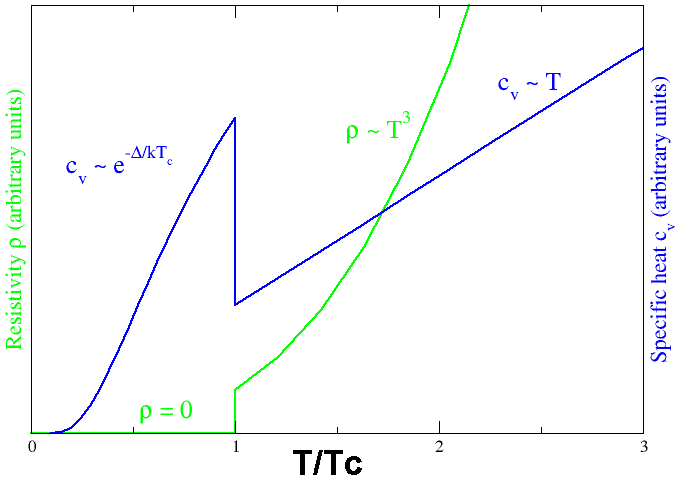
\includegraphics[width=0.65\textwidth]{immagini/andamento_calore_specifico_in_funzione_della_temperatura.png}
   \caption*{Andamento del calore specifico (in blu) e della resistività (in verde) per un superconduttore in funzione della temperatura.}
\end{figure}
\hspace{-0.6cm}Osserviamo che sopra la temperatura critica, il comportamento è quello tipico dei sistemi metallici, con una dipendenza lineare della capacità termica dalla temperatura. Tuttavia, alla temperatura critica, si verifica una discontinuità nel calore specifico, seguita, a temperature inferiori, da un comportamento completamente diverso. In particolare, a basse temperature, il calore specifico segue una dipendenza di tipo esponenziale, il che suggerisce l'emergere di una nuova scala energetica nel sistema, fatto che vediamo chiaramente nella forma $\exp(-\text{energia}/k_B T_c)$. La presenza di questa dipendenza esponenziale indica che entra in gioco una nuova scala di energia, che chiamiamo $\Delta$. Scopriremo che essa rappresenta una misura della gap energetica nello spettro di un superconduttore. Infatti, nello spettro energetico di un superconduttore, esiste un intervallo di energia proibito per le eccitazioni.\\
Il concetto di gap energetico è analogo a quello dei semiconduttori, ma il meccanismo fisico che lo genera è completamente diverso.
%We see that above the critical temperature we have a behavior which is typical of the metallic systems, so linear in temperature, we have a discontinuity of the specific heat at the critical temperature and then for lower temperatures we have a completely different temperature dependence on the specific heat which is, and this is true particularly for small temperatures, an exponential type, and is an indicative of a new energy scale coming into place, because we have a dependence in the form of the exponential to the minus some energy divided by $k_BT_c$. The fact that we have this type of exponential behavior which describes this dependence indicates that there is some new energy scale coming into play. This energy scale is what we call $\Delta$, which we are going to see is a measure of the gap we have in the energy spectrum of a superconductor. In fact, we are going to see that in the spectrum of a superconductor we have an energy regime for excitations of the superconductor which is forbidden. The concept of energy gap in the energy spectrum is analogous to what we have in a semiconductor, but the process is totally different.\\
In questo grafico vediamo anche a sinistra il comportamento della resistività in un superconduttore. Osserviamo che è zero per temperature inferiori alla temperatura critica, mentre per temperature superiori la resistività segue il comportamento tipico dei sistemi elettronici, con una dipendenza dalla temperatura di $T^3$.
\subsection{Gap nello spettro di eccitazione}
Come abbiamo detto, il comportamento esponenziale del calore specifico indica la presenza di un gap nello spettro, il che significa che la densità degli stati all'energia di Fermi presenta un intervallo di energie proibite:
\begin{figure}[H]
   \centering
   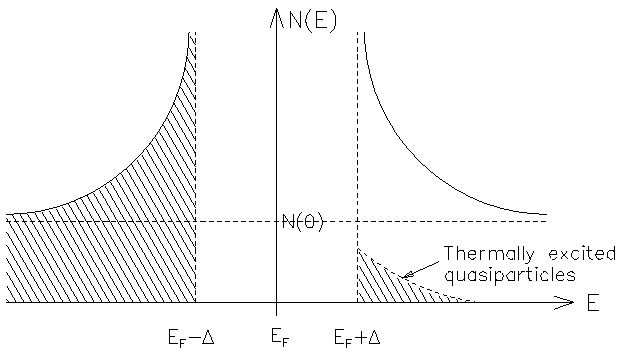
\includegraphics[width=.8\textwidth]{immagini/Densita_degli_stati_superconduttore.png}
\end{figure}
%This gap depends on temperature and it becomes zero at the critical temperature. Basically, what happens increasing the temperature going from zero temperature to the critical temperature is that at the critical temperature the superconductor becomes again a normal metal and then the density of states becomes the one we know for a normal metal. We can see the behavior of the gap as a function of temperature with this gap closing at the critical temperature in the following picture:
\hspace{-0.6cm}Questo gap dipende dalla temperatura e si annulla alla temperatura critica. In pratica, ciò che accade aumentando la temperatura da zero fino alla temperatura critica è che, alla temperatura critica, il superconduttore ritorna ad essere un metallo normale, e la densità degli stati torna ad essere quella che conosciamo per un metallo normale. In altre parole, man mano che aumentiamo la temperatura il gap si restringe, fino a chiudersi in corrispondenza della temperatura critica.\\
Possiamo osservare l'andamento del gap in funzione della temperatura, che si chiude alla temperatura critica, nella seguente figura:
\begin{figure}[H]
   \centering
   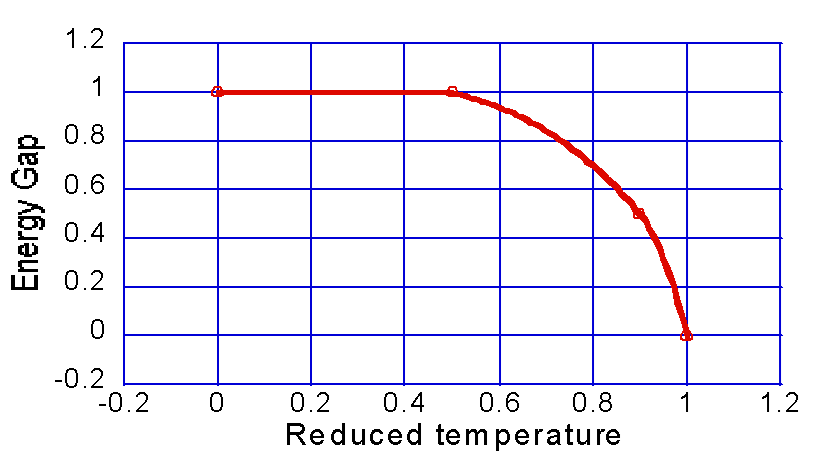
\includegraphics[width=.6\textwidth]{immagini/Andamento_gap_in_funzione_di_T.png}
   \caption*{Andamento del rapporto $\frac{\Delta(T)}{\Delta(0)}$ in funzione della temperatura ridotta $\frac{T}{T_c}$.}
\end{figure}
%The appearance of a gap in the spectrum has also other evidences. In particular, another evidence comes from the spectroscopic measurements of the absorption of electromagnetic radiation by a superconductor. In general, if we have a material and we make it interact with the electromagnetic field, what happens is that some frequencies are absorbed and the absorption spectrum depends intrinsically on the spectrum of the material hence on its density of states. If there are gaps in the spectrum, it means that the system cannot absorb energies smaller than the energy gap, and indeed measurements of absorption of electromagnetic radiation by a superconductor relieved that there was an onset of absorption for frequencies which are larger than an energy scale. Moreover this energy scale, which now we know is related to the superconducting gap, was scaled with the critical temperature, with a very simple expression: $\hbar\omega \approx k_B T_c$. So this experiment, which came out a little bit later with respect to the first observation, are part of the indication of the fact that in the spectrum of the superconductor there are some energies which cannot be taken simply because the system material is not able to absorb energy smaller than an energy scale, which is proportional to $k_B T_c$.\\
\hspace{-0.6cm}La comparsa di un gap nello spettro ha anche altre evidenze sperimentali. In particolare, un'altra evidenza proviene da misure spettroscopiche dell'assorbimento di radiazione elettromagnetica da parte di un superconduttore. In generale, se abbiamo un materiale e lo facciamo interagire con un campo elettromagnetico, ciò che accade è che alcune frequenze vengono assorbite, e lo spettro di assorbimento dipende intrinsecamente dallo spettro del materiale, e quindi dalla sua densità degli stati. Se ci sono dei gap nello spettro, significa che il sistema non può assorbire energie inferiori al valore del gap, e infatti le misure di assorbimento di radiazione elettromagnetica da parte di un superconduttore hanno rivelato che l'assorbimento inizia solo per frequenze superiori a una certa scala energetica. Inoltre, questa scala energetica (che ora sappiamo essere legata al gap superconduttivo) risultava proporzionale alla temperatura critica, secondo la relazione $\hbar \omega \approx k_B T_c$.\\
Questi esperimenti, che sono arrivati poco dopo le prime osservazioni del fenomeno, sono una chiara indicazione del fatto che nello spettro di un superconduttore esistono energie che non possono essere assorbite, semplicemente perché il materiale non è in grado di assorbire energia al di sotto di una determinata soglia, proporzionale a $k_B T_c$.\\
%Another evidence of this gap in the spectrum comes from the measurements of current--voltage relation, that is the relation between the current flowing in a superconducting material varying the applied voltage difference. These experiments were not done on a single superconductor but in a structure, which we will study in more depth in the following, which is composed by a normal metal, then some barrier so some insulating layer, and a superconducting material like the following picture:
Un'altra evidenza della presenza del gap nello spettro proviene dalle misure della relazione corrente--tensione, cioè dalla relazione tra la corrente che fluisce in un materiale superconduttore al variare della differenza di potenziale applicata.
Questi esperimenti non sono stati condotti su un singolo superconduttore, ma su una struttura (che analizzeremo più in dettaglio in seguito) composta da un metallo normale seguito da una barriera (ossia uno strato isolante) e infine da un materiale superconduttore. Vediamo la struttura dei livelli energetici di una tale configurazione:
\begin{figure}[H]
   \centering
   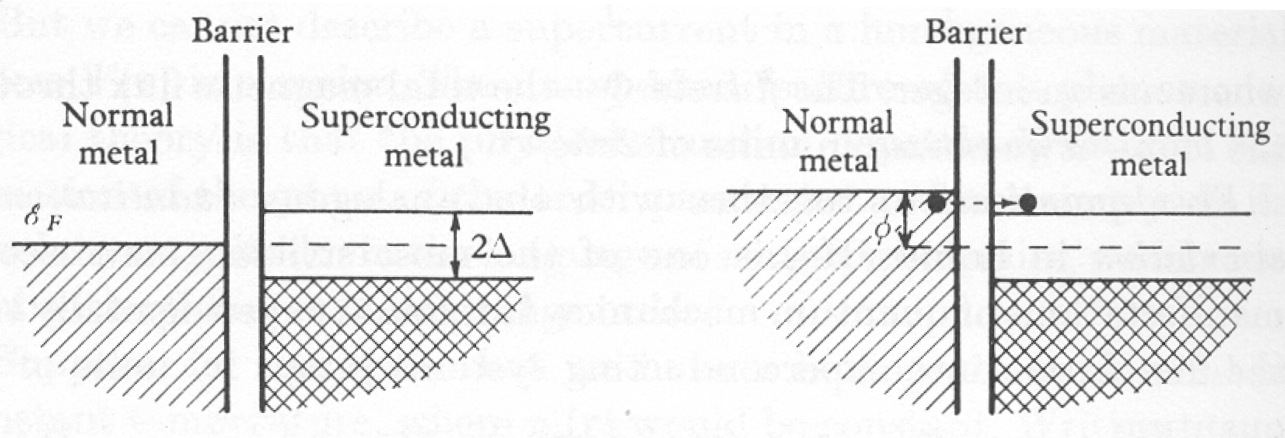
\includegraphics[width=.9\textwidth]{immagini/Electron_tunneling.png}
\end{figure}
%As we know, for a normal metal at zero temperature all the levels up to the Fermi energy are filled, and above there are all levels accessible by excitation. If instead in the superconductor\mn{Let's remark that at this stage we still don't know the reason, so we're assuming the superconductive spectrum has this gap.} we have all the levels filled up to some energy, and then there is an energy gap which separates the allowed states, and if the the levels of the two materials are like in the left configuration, if we do not apply a voltage between them an electron of the metal near the Fermi energy cannot pass\mn{This passing from one side to the other means passing an area where there is an insulating material that in terms of quantum mechanics represents a potential barrier, so this passage from one side to the other is by a quantum mechanical tunneling through a potential barrier.} to the other side because it doesn't have an available state on the other side.\\
%If we apply a potential difference, which can be described as a relative shift of the energy levels, in such a way that the Fermi level on the left-hand side is aligned, using the language of semiconductors, with the lower level of the upper band, so if we have a situation like the one in the right, under this condition an electron of the metal can tunnel through the barrier and find an available energy state on the other side. This means that if we want to see how the current--voltage characteristics looks like, this behavior means that if the voltage is smaller than an energy of the order of $\Delta$, there cannot be current because there are no available states on the other side, so there is zero current, and if the voltage is sufficient to unbalance the two bands in the proper way, at this point there will be a current flowing. So what we observe is a behavior like this:
\hspace{-0.6cm}Come sappiamo, per un metallo normale a temperatura nulla, tutti i livelli fino all'energia di Fermi sono occupati, e al di sopra ci sono tutti i livelli accessibili tramite eccitazione.
Nel superconduttore\sn{Ricordiamo che a questo punto non conosciamo ancora la causa di questo comportamento: stiamo semplicemente assumendo che lo spettro di un superconduttore presenti un gap.}, invece, tutti i livelli sono occupati fino a una certa energia, e poi c'è un intervallo di energia proibito che separa gli stati permessi. Se i livelli energetici dei due materiali sono disposti come nella configurazione a sinistra, in assenza di una differenza di potenziale tra loro, un elettrone nel metallo vicino al livello di Fermi non può passare dall'altra parte\sn{Questo passaggio da un lato all'altro significa attraversare una regione in cui è presente un materiale isolante, che in termini della meccanica quantistica rappresenta una barriera di potenziale e quindi il passaggio è un effetto di tunneling quantistico attraverso una barriera.}. Se applichiamo una differenza di potenziale, che può essere descritta come uno spostamento relativo dei livelli energetici, in modo che il livello di Fermi sul lato sinistro sia allineato, usando il linguaggio dei semiconduttori, con il livello inferiore della banda superiore, cioè in una configurazione come quella mostrata a destra, allora un elettrone del metallo può attraversare la barriera tramite tunneling e trovare uno stato disponibile sull'altro lato.\\
Ciò implica che finché la tensione applicata è inferiore a un'energia dell'ordine di $\Delta$ non può esserci passaggio di corrente, perché non ci sono stati accessibili sull'altro lato. Quando invece la tensione è sufficiente a sbilanciare in maniera opportuna i due spettri, inizia ad esserci passaggio di corrente. Pertanto, il comportamento corrente--tensione che si osserva sperimentalmente è come quello riportato nel seguente grafico:
\begin{figure}[H]
   \centering
   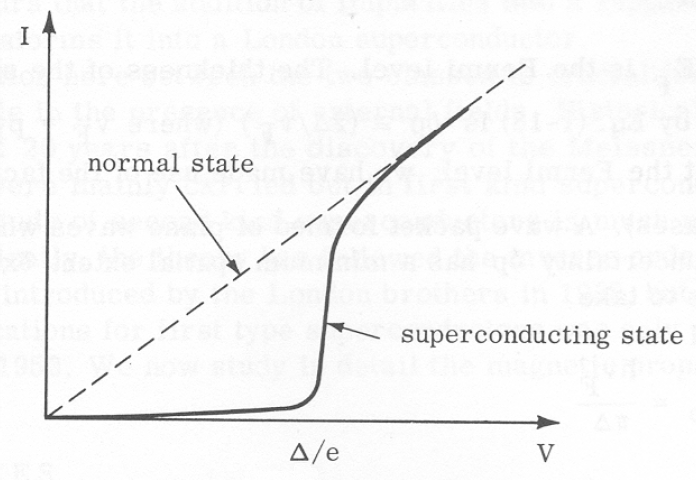
\includegraphics[width=.6\textwidth]{immagini/Grafico_tensione_corrente_Electron_tunneling.png}
\end{figure}
\hspace{-0.6cm}Come possiamo vedere, c'è una variazione brusca della corrente vicino a un'energia che è proporzionale al gap energetico. Se aumentiamo ulteriormente la tensione, il che significa che sbilanciamo ulteriormente i livelli energetici, possiamo, in un certo senso, dimenticare che un materiale è superconduttore ed è come se avessimo semplicemente due metalli normali, con il tunneling elettronico che può avvenire, quindi abbiamo una caratteristica corrente-tensione lineare, come in un sistema ohmico.\\
Questo comportamento, in cui si ha il passaggio di corrente soltanto se la differenza di potenziale supera un certo valore, è detto di attivazione. La presenza di questo comportamento ci porta a pensare che nello spettro di un materiale superconduttore ci sia un gap.
\subsection{Effetto isotopico}
%Another peculiarity of superconductors is called isotope effect. It was observed that the critical temperature to which the material becomes superconductive, depends on the mass of the isotope of the material. In other words, different isotopes of the same material have different critical temperature, following the law
%with $\alpha \approx 0.5$.\\
%The various isotopes differ from each other for the mass of the ions, which form the lattice of the material. So it's not the property of the electrons in the material, but of the lattice. This was quite astonishing because it indicated that superconducting phase transition, a property which is intrinsically related to electromagnetic properties, so conduction properties, which we are used to relate to electrons, depends on properties of the lattice. This fact was completely unexplained until Frölich in 1950, had the intuition that the mechanism behind superconductivity might be related to the interaction of electrons with the phonons, so with the lattice vibrations. This was the precise intuition which led Bardeen, Cooper and Schrieffer to develop their theory which is based on the idea that two electrons with opposite charge and momentum can actually interact with an attractive interaction which comes from the common interaction with the lattice. We will see more precisely later on, but we have to keep in mind that the isotope effect was the incipit which gave the idea that some mechanism of interaction between electrons and phonons could be the key to the superconductivity.
Un'altra peculiarità dei superconduttori è chiamata effetto isotopico. È stato osservato che la temperatura critica alla quale il materiale diventa superconduttore dipende dalla massa dell'isotopo del materiale. In altre parole, isotopi diversi dello stesso materiale presentano temperature critiche diverse, seguendo la legge:
\begin{equation*}
   T_c \propto M^{-\alpha}
\end{equation*}
con $\alpha \approx 0.5$.\\
I diversi isotopi si distinguono tra loro per la massa degli ioni che costituiscono il reticolo del materiale, quindi non si tratta di una proprietà degli elettroni nel materiale, ma del reticolo stesso. Questo fatto fu piuttosto sorprendente, perché indicava che la transizione alla fase superconduttiva, cioè una proprietà intrinsecamente legata all'elettromagnetismo, quindi alla conduzione elettrica, che siamo abituati ad associare agli elettroni, dipende invece da una proprietà del reticolo.\\
Questo fatto rimase del tutto inspiegato fino a quando, nel 1950, Fröhlich ebbe l'intuizione che il meccanismo alla base della superconduttività potesse essere legato all'interazione degli elettroni con i fononi, ovvero con le vibrazioni del reticolo. Questa fu l'intuizione decisiva che portò Bardeen, Cooper e Schrieffer a sviluppare la loro teoria, basata sull'idea che due elettroni con carica e momento opposti possano interagire tra loro attraverso un'interazione attrattiva mediata dall'interazione comune con il reticolo.\\
Vedremo più in dettaglio questo aspetto in seguito, ma dobbiamo tenere a mente che l'effetto isotopico fu l'elemento iniziale che fece intuire che un meccanismo di interazione tra elettroni e fononi potesse essere la chiave per spiegare la superconduttività.
%\subsubsection*{Altre informazioni sugli elementi superconduttori (da sistemare)}
%, so this is what we want to tell. we think there are some more information. , from the periodic table, you can now see how many materials in this placement of activity. And you can see the colors are all superconductive materials. So they are not just the standard aluminum, they could be, et cetera. But a large number of materials are superconductive, either under ambient pressure or under high pressure. And this is the reason for the colors. You see here the different temperatures. These are called small temperatures. So, let's say the materials from the periodic table are typically low-temperature materials. But if we analyze the this is, for instance, starting with a stable, the different materials which by now is placed by conductivity, we see that beside elements which are the ones we can find in the periodic table, there are also compounds which display superconductive behavior. And in particular, these compounds, which are typically ceramic materials, display superconductivity at much higher temperatures. You see that here we reach 100 Kelvin. So, much higher temperature with respect to the conventional or normal temperatures. These materials are called high-temperature superconductors. We won't enter the limits of the high-temperature superconductors, also because the theory behind high-temperature superconductors is not totally accepted. But this is just to show you this graph you see as a function of years, the different critical temperatures.
%\begin{figure}[H]
%   \centering
%   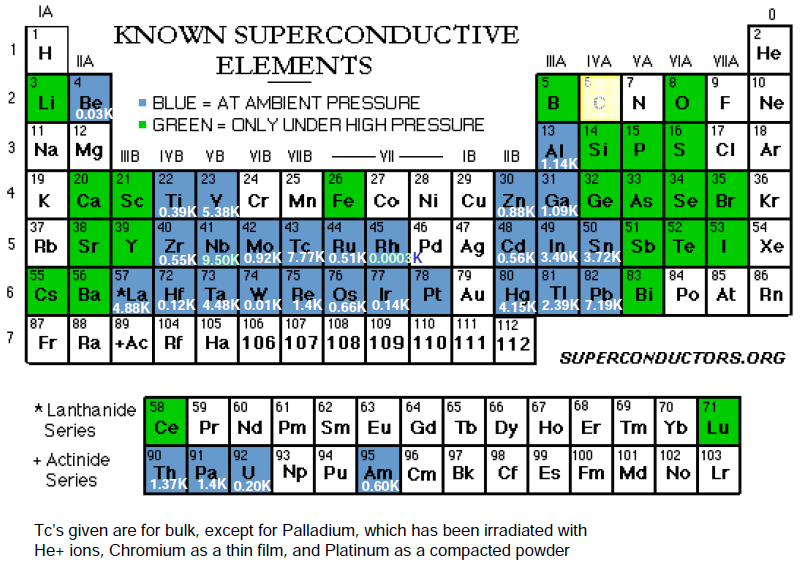
\includegraphics[width=.8\textwidth]{immagini/Tabella_elementi_superconduttivi.png}
%\end{figure}
%You see that there was a there were also were the 80s, late 80s, a discovery of these materials, which are based on they are basically some of the they are ceramic and are characterized by having layered structures of copper or oxide planes, which are separated by layers of, so to speak, chargers and warzones, which are your materials like, and the ones you see here. So, yeah, they have this layered structure and they display superconductivity but at much higher temperatures with respect to the bare elements. The theory behind high-temperature superconductors is not totally accepted, and particularly is not clear, which is the mechanism which needs the superconductivity, so we will not enter this part where you write to know the process of superconductivity in the view that also exists high-temperature superconductivity, and you keep in mind that the mechanism behind that is considerably different from the microscopic one, which we are now going to describe in the next lectures. And, , this is just a summary of what we have said today, and the interest, just to say that the interest for high-temperature superconductors, of course, comes from the applications, because we would really, of course, materials which are zero resistivity and in this phase, a temperature which are much higher than the cryogenic temperatures are, of course, interesting for all applications. So, there is clearly an interesting understanding in using these materials, but still there are some contrasts in using them. First of all, the fact that these players material are very sensitive to fluctuations, and so it means that they are not stable enough to allow an explosion in them, and you understand. , so we think that for the moment we , we will, maybe next time, we discuss about the qualitative features of the experiment. , so today we stop here, and the slides that are available, we have only done a new overview of phenomenology, and what is important to have in mind is, let's say, the only thing that we have done is to introduce the thermodynamic potentials that allow us to describe the transition, in particular the energy for the teams, and this has allowed us to introduce the thermodynamic definition of the field. This part here is good, because we will use it in the description of the theory of Ginzburg--Landau, which is based on the theory of Landau and the transition of phases. The second tip is that we that use the terminology and the terms of free energy, and the transition of things. So, this part here is important for the work of the idea of the experiment. And to address the thermodynamic potential, the difference between the fact that the Meissner effect cannot be explained with a perfectly conductive behavior and a simple explanation based on the analysis of the law of doing a perfect conductor, a simple point of point to understand the difference. . . No, no, no. So, a conductor is not a perfect conductor, because this is not is But to say resistivity with nothing resistivity. Yes. , perfect. The resistivity is zero of the first equation, which is that this resistivity has nothing to do with the Meissner effect, that is, the response to a magnetic field is not perfect. This is perfect. It is not a perfect conductor. It conductor. It conductor. perfect conductor that loses its internal voltage if this field is the last one. Yes, yes. We have this one, which means that a master should be able to see the distance.
%\section{Superfluidità (da sistemare)}
%Superfluidity is the property which some systems, actually $\rm ^3He$ and $\rm ^3He$ so far, which under proper conditions of temperature, magnetic field and pressure sustain the flow without friction, in the sense of without any viscosity. This takes place for certain temperatures as we said and up to certain transport velocities that are in this room. Now today, the only materials which display this Bm are $\rm ^4 He$ and $\rm ^3 He$. The first one is superfluid at about 2 K, the second one at much smaller temperature, and indeed it was discovered some years ago. And the experiments which demonstrated this superfluid behavior are again, also in this case, online, called thermodynamic and off-transport. Actually what was surprising and was to some extent is still not completely understood is the the that these two isotopes of helium are actually characterized by many different statistics, not only different atomic masses. And this of course makes the understanding of the phenomenon quite complicated. In particular, as we said, $\rm ^4 He$ has zero nuclear spin, therefore it's the bosonic natural base, those are statistics, whereas $\rm ^3 He$ has a nuclear spin which is an integer, so it obeys the media statistics. Now the first experiments, so helium-4, was done in 1930 by Fabitza, and the property was related to, it was a transport property, and it concerned the transport of helium through a narrow cabilla, and it was possible to see that this transport through this narrow cabilla was placed without any friction. And how did they understand that there was no friction, simply because for a viscous, it would be a fluid, a normal fluid, there is a connection between the difference in pressures on the two sides of the cabilla, and the coefficients eta, which describes this possibility. And actually what it was observed is that under this condition, there was no change in the pressure on the two sides of the cabilla, which was an indication of the fact that there was a super fluid. The other property, which is a game of sort of mechanical origin, is the observation of a stack of different disks, which were immersed in helium, and it was possible to see that the torsional, the torsional properties, so the oscillation frequency of this task, or stack of disks, was depending on the temperature of the system overall, and it appeared that for temperature below a certain value, the moment the inertia of the disk was changing, and this inertia was changing in such a way that apparently part of the disks were not involved. So this means, this is due to the fact that there is this fluid, which which in between the disks, becomes super fluid, and then the overall stack of disks is not anymore as single as the object, as it would be if there was a friction, but they were almost independently moving. So this was another indication. So these are, so to speak, mechanical mechanical The other peculiar feature of the loophole is the phase diagram, and in the phase diagram, which is shown out there, we have the pressure and the temperature, and the peculiarity is the following. So we have these different phases, which are a solid phase, for small temperature and sufficiently high pressure. We have a normal liquid behavior for pressure and temperature above certain pressure, but for small temperatures and for small values of the pressure, there is a super fluid behavior. And in particular, we see that differently from the usual transition we have in a fluid, where we have a tripod point between the three phases, there is no tripod point in this case. There is a liquid phase down to zero, which is surprising. And moreover, there is the peculiarity in the dependence on this phase, which separates this line, which separates the two phases, which is flat. And this is a relevant information because the dependence of the pressure on the temperature enters the entropy. So if we have a flat dependence on the pressure on the temperature, it means that there is no change in the entropy. Or if you want, this is a line where the entropy does not change, which indicates that we are passing from the liquid, the solid, there is no change in entropy. So it means that it gives us information about the structure, if you want, of the liquid, meaning that it has the same symmetry, the same entropy, the same order, the little profile of the solid phase.
%So this is quite the peculiarity. Moreover, if we, the space diagram translates in a peculiar dependence on the specific heat, of the specific heat of temperature, with a T-cube behavior, as more temperatures, which is different from what one observed for a bosonic condensation, you don't know, but just to notice that this is not the same as it happens in a bosonic condensation, which in principle, one may, at first instance, one could think that being a bosonic system, the same mechanism could happen, also in this case, but this is not the case. And the dependence of the specific heat on temperature is an indication that this is not the case. And moreover, there is this peculiar sort of spike here at the critical temperature, at the transition point. This point is called the lambda point, because of the shape of this curve. And this peculiar algebraic behavior close to the critical temperature, this type of behavior is an indication of the fact that between the normal liquid and the superfluid, there is a phase transition with two components of the parameter. Again, this is something which is not obvious, I'll just say with this problem, at this moment, just to let you know that there is some peculiar model behind this type of transition. , so these are just hints of the fact that in addition to the properties of a superconductor, which we have seen of Lady, are to the resistivity and the dependence and the expulsion of the documented field out of the sample, superfluids have quite different properties, quite different evidence in experiments both in transport, mechanical response, and in thermal properties. As you can see also in this case, the thermal properties are very important. Similarly, we have seen in the report a very important indicator of a transition, the characteristics of the transition. We will come later to the explanation with different features. At this stage, just to give you an idea of the variety of phenomena, which indicated some peculiar property, some peculiar phenomenon. 
\section{Equazione di London}
Iniziamo la trattazione dei superconduttori partendo dalle teorie fenomenologiche. Il motivo per cui utilizziamo queste ultime non è solo storico, ma anche perché si tratta di modelli semplici che permettono comunque di descrivere una grande varietà di fenomeni e che vengono ancora utilizzati per analizzare dispositivi superconduttivi semplici.\\
La prima teoria fenomenologica è l'equazione di London, formulata dai fratelli London nel 1935. Fu la prima teoria in grado di spiegare l'espulsione del campo magnetico dai superconduttori, ovvero l'effetto Meissner. L'idea alla base di questa teoria è molto semplice: i London furono motivati dall'osservazione che, al di sotto di una certa temperatura, la resistività del mercurio diventava nulla. L'ipotesi più immediata che si potesse fare era che il metallo fosse composto da elettroni suddivisi in due "fluidi", con una parte di elettroni che si comportava come normali elettroni, quindi con resistività finita, e un'altra parte che per qualche ragione diventava superconduttiva. L'idea è quindi che la densità totale di elettroni sia data dalla somma di un contributo normale $n_n$ e di un contributo superconduttivo $n_s$:
\begin{equation}
   n=n_n + n_s
   \label{eq:densita_elettroni}
\end{equation}
Tale modello a due fluidi si ispirava a un modello già proposto per l'$^4\rm He$, ma per ora possiamo accantonare questo aspetto.\\
L'assunzione fondamentale del modello di London è, dunque, che in un superconduttore coesistano elettroni normali ed elettroni superconduttivi. Se immaginiamo un sistema composto da due componenti fluide, e assumiamo che al di sotto della temperatura critica la componente superconduttiva sia presente, allora possiamo trattare il contributo degli elettroni normali e superconduttori come un sistema di trasporto con due canali in parallelo. Chiaramente, se uno dei due canali ha resistività nulla mentre l'altro ha resistività finita, il trasporto della corrente avverrà interamente attraverso il canale a resistività nulla. Viceversa, quando il sistema supera la temperatura critica o quando le condizioni del campo magnetico sono tali che il materiale si trova in fase normale, rimane un unico canale con resistività finita, e il materiale si comporta come un normale conduttore. Il motivo per cui la modellizzazione del problema è questa è che la teoria di London si propone di spiegare la fenomenologia superconduttiva, e questa fenomenologia include il fatto che se aumentiamo la temperatura nel materiale avviene il passaggio da superconduttore a metallo normale. Quindi, se abbiamo due fluidi con questi due comportamenti diversi al di sotto della temperatura critica, gli "elettroni superconduttivi" sono quelli responsabili della corrente.\mn{Ciò che avviene è che gli elettroni superconduttivi "cortocircuitano" gli elettroni normali e fanno crollare la resistività a zero. \cite{Annett}}
%We talk about superconductors starting from phenomenological theories. The reason why we use these phenomenological theories until now are not just for historical reasons, but also because they are simple theories which still allow us to describe a variety of phenomena which still we use when we consider very simple superconducting devices.\\
%The first phenomenological theory is the London equation, it's due to the London brothers on 1935. It was the first theory which could explain the expulsion of the magnetic field out of the superconductors, that is the Meissner effect. The idea behind this is very simple: they were motivated by the observation that below some certain temperature, the resistivity of Mercury went to 0, and the simplest instance which one could suppose is that the metal was formed by electrons described as two fluids, so considering part of the electrons behaving for some reason as normal electrons, so with normal resistivity and another part which for some unknown reason became superconductive. So, the idea is that we have a density of electrons given by a normal contribution plus a superconducting contribution. This two-fluid model was actually motivated from what was already proposed for $\rm ^4 He$, but let's keep it on one side of our mind. So the basic assumption of this London model is that in a superconductor, we have at the same time normal electrons with some density, which we call $n_n$, and superconducting electrons with some other density, which we call $n_s$. The total density is then given by
%\begin{equation*}
%   n=n_n + n_s
%\end{equation*}
%The idea is that if we have a system where we have these two fluid components, if for some reason (and this is the assumption) the superconducting component below the critical temperature is present, then we can think to the contribution of this normal and superconducting elements like a sort of parallel combination of two channels for transport. Clearly, if there is a channel which is with zero resistivity and the other with a finite resistivity, the transport takes place through the zero resistivity channel. Whereas, when the system is above the critical temperature or we have proper condition for the magnetic field such that it becomes normal, then we have a single channel with some resistivity and then we have the normal behavior, because this model is aimed to try to give an explanation of the superconducting phenomenology, and the phenomenology includes the fact that if we increase the temperature then the transition from superconducting to normal takes place in the material. So, if we have two fluids with these two different behaviors below the critical temperature, the "superconducting electrons" are the ones which are responsible for the current.
\subsection{Prima equazione di London}
%The equation which describes the supercurrent density is
%which tells us that current density is proportional to the vector potential with a coefficient which depends on the density of superconducting electrons, the charge of a single electron and the mass of a single electron.\\
%\eqrefcustom{eq:prima_equazione_di_London} is not enough: it applies in this model provided we are in a proper gauge, and in particular in the gauge which is called London gauge, which is characterized by having $\div{\vb{A}}=0$.\\
%Let's now try to understand how this equation comes from, which is the reason behind, and why it describes superconducting behavior and Meissner effect. Within this phenomenological model, this equation is the corresponding of Ohm's law for normal conductors, which states that for a normal conductor the current density is given by $\vb{J}=\sigma \vb{E}$. The idea is that if we have a superconductor this equation does not apply, because for $\rho \to 0$ we have $\sigma \to \infty$, which has not physical meaning. So Ohm's law has to be replaced by \eqrefcustom{eq:prima_equazione_di_London}.\\
%Now let's see how this equation comes from.\mn{Obviously, \eqrefcustom{eq:prima_equazione_di_London} is a phenomenological equation, so there is not a rigorous derivation, but of course the two London didn't invent it out of the blue: there is some reasoning behind it, so we will follow this reasoning and understand how we can describe the two characteristic phenomena, and then we will see some predictions from this.}\\
L'equazione che descrive la densità di corrente superconduttiva è la prima equazione di London, la quale afferma che
\begin{equation}
   \vb{J}=-\frac{n_s e^2}{m_e} \vb{A}
   \label{eq:prima_equazione_di_London}
\end{equation}
ossia che la densità di corrente è proporzionale al potenziale vettore $\vb{A}$ tramite un coefficiente che dipende dalla densità di elettroni superconduttivi $n_s$, dalla carica dell'elettrone $e$ e dalla sua massa $m_e$.\\
L'\eqrefcustom{eq:prima_equazione_di_London} da sola non basta: essa è valida all'interno di questo modello a patto di scegliere una gauge opportuna che è la gauge di London, caratterizzata dalla condizione $\div{\vb{A}} = 0$.\\
Vediamo da dove proviene la necessità di scegliere tale gauge. Sappiamo che, in generale, vale l'equazione di continuità:
\begin{equation*}
   \pdv{\rho}{t} + \div{\vb{J}} = 0
\end{equation*}
Se ci troviamo in condizioni di corrente continua (DC), allora $\pdv*{\rho}{t}=0$, e l'equazione di continuità diventa $\div{\vb{J}}=0$. Se inoltre $\vb{J}$ è proporzionale ad $\vb{A}$, come supposto dall'equazione di London, allora necessariamente deve valere anche $\div{\vb{A}}=0$, che è proprio la gauge di London. Quindi, la necessità di scegliere tale gauge nasce direttamente dall'assunzione di una densità di corrente proporzionale ad $\vb{A}$, insieme alla condizione di corrente continua.\\
All'interno di questo modello fenomenologico, questa equazione rappresenta l'equivalente della legge di Ohm per i conduttori normali, la quale stabilisce che in un conduttore normale la densità di corrente è data da $\vb{J}=\sigma \vb{E}$. L'idea è che se abbiamo un superconduttore, questa equazione non è più valida, perché nel limite di resistività nulla $\rho \to 0$, la conduttività $\sigma$ diverge, $\sigma \to \infty$, il che non ha significato fisico. Quindi la legge di Ohm deve essere sostituita dall'\eqrefcustom{eq:prima_equazione_di_London}.
\subsection{Derivazione dell'equazione di London}
Vediamo ora da dove proviene questa equazione, quale ne è il fondamento e perché descrive il comportamento superconduttivo e l'effetto Meissner. Prima di proseguire, va notato che tale equazione è stata ricavata anche dalla teoria BCS circa vent'anni dopo. Questo fatto ci dà un'indicazione di quanto essa sia rilevante: pur essendo stata ottenuta, come vedremo, sotto ipotesi non del tutto giustificate e principalmente motivata dal bisogno di avere una teoria fenomenologica capace di spiegare i risultati sperimentali, essa può comunque essere dedotta anche da una teoria microscopica. Questo fornisce quindi una giustificazione del perché questa equazione rimanga valida: non è solo un'intuizione empirica, ma trova fondamento anche in una descrizione teorica più profonda.\\
Cerchiamo innanzitutto di capire come si giunge a questa equazione.\sn{Ovviamente, l'\eqrefcustom{eq:prima_equazione_di_London} è un'equazione fenomenologica, quindi non esiste una derivazione rigorosa, ma chiaramente i fratelli London non l'hanno inventata dal nulla: c'è un ragionamento alla base, che ora seguiremo per capire come essa descriva i due fenomeni caratteristici della superconduttività, e vedremo anche alcune previsioni che ne derivano.}
Partiamo dalla considerazione che, tipicamente, ciò che diventa superconduttore è un metallo, e sappiamo che in un metallo, in condizioni normali, vale la legge di Ohm, cioè $\vb{J} = \sigma \vb{E}$. Questa equazione è valida fisicamente non solo in condizioni statiche, ma anche in presenza di variazioni temporali. Se, come di consueto per un metallo normale, vogliamo comprendere la risposta a un campo variabile nel tempo, ciò che facciamo è sviluppare in serie di Fourier sia il campo elettrico che la densità di corrente. Sappiamo quindi che, per valori finiti della frequenza, la risposta ha la forma:
\begin{equation}
   \vb{J} e^{-i\omega t}
   =\sigma(\omega) \vb{E} e^{-i\omega t}
   \label{eq:legge_di_Ohm_in_sviluppo_di_Fourier}
\end{equation}
La conducibilità dipende dalla frequenza. La sua forma esplicita deriva da una descrizione classica ed è data da:
\begin{equation*}
   \sigma(\omega)
   =\frac{n e^2 \tau}{m_e} \frac{1}{1 - i \omega \tau}
\end{equation*}
dove:
\begin{itemize}[leftmargin=0.5cm]
   \item $n$ è la densità di portatori di carica, che in un metallo normale sono gli elettroni normali;
   \item $e$ è la carica degli elettroni;
   \item $m_e$ è la massa degli elettroni\mn{Per convenzione, in questa definizione si usa la massa dell'elettrone libero nel vuoto, $m_e$, piuttosto che la massa efficace $m$.};
   \item $\tau$ è il tempo di vita medio degli elettroni mentre si muovono nel conduttore. Si tratta di un tempo di vita perché, nel modello di Drude, gli elettroni subiscono urti con gli ioni del reticolo e tra di loro, e $\tau$ rappresenta l'intervallo medio tra questi urti.
\end{itemize}
Come possiamo vedere, essa è una quantità complessa, dove la parte reale rappresenta la risposta resistiva del conduttore, mentre la parte immaginaria rappresenta la risposta induttiva. Quello che allora faremo adesso è separare la parte reale da quella immaginaria. L'idea è che, all'interno di questo modello, ci si aspetta che quando il materiale diventa superconduttore il tempo medio tra una collisione e l'altra diventi estremamente lungo, tendendo all'infinito. In questo limite, si ottiene che la risposta reale, cioè la parte reale della conducibilità che corrisponde alla risposta resistiva, tende a zero, e rimane soltanto la componente immaginaria. Questo è esattamente ciò che accade, e ora vedremo come funziona.\\
La parte reale della conducibilità è:
\begin{equation*}
   \Re [ \sigma(\omega) ]
   =\frac{n e^2 \tau}{m_e} \frac{1}{1 + \omega^2 \tau^2}
\end{equation*}
%It's clear that if $\tau \to \infty$ then $\Re [ \sigma(\omega) ] \to 0$ and this is what we expect for a normal conductor: if the average time between collisions goes to infinity, the material is not resistive anymore and we only have the imaginary response.\\
%Let's come back to the case when we have a finite $\tau$. In this case, we also have what is called the sum rule, that says
%that is integrating over frequency $\Re [ \sigma(\omega) ]$ as a function of $\omega$ we get a constant independent of the lifetime $\tau$. This comes from the fact that if we look at this real part of the conductivity as a function of $\omega$, this is simply a Lorentzian which is centered in $\omega=0$ and with a width equal to $1/\tau$ and a maximum height equal to $\tau$.
È chiaro che se $\tau \to \infty$, allora $\Re [ \sigma(\omega) ] \to 0$, e questo è esattamente ciò che ci aspettiamo per un conduttore normale: se il tempo medio tra le collisioni tende all'infinito, il materiale non è più resistivo e rimane soltanto la parte immaginaria.\\
Torniamo ora al caso in cui $\tau$ è finito. In questo caso, vale anche quella che viene chiamata "sum rule" (regola di somma), che afferma:
\begin{equation*}
   \int_{-\infty}^{+\infty} \dd{\omega} \Re [ \sigma(\omega) ]
   =\frac{\pi n e^2}{m_e}
\end{equation*}
cioè, integrando rispetto alla frequenza la parte reale della conducibilità $\Re [ \sigma(\omega) ]$ come funzione di $\omega$, si ottiene una costante indipendente dal tempo di vita $\tau$. Ciò deriva dal fatto che, se consideriamo $\Re [ \sigma(\omega) ]$ come funzione di $\omega$, essa è semplicemente una curva lorentziana centrata in $\omega=0$, con una larghezza pari a $1/\tau$ e un'altezza massima pari a $\tau$.\\
Il fatto che l'integrale sia indipendente dal valore di $\tau$ significa che, anche se abbiamo questo comportamento limite in cui $\tau \to \infty$, questa sum rule deve comunque essere rispettata. Questo implica che tale relazione dovrebbe rimanere valida qualunque sia il valore di $\tau$. Tuttavia, abbiamo visto che per $\tau \to \infty$ la parte reale di $\sigma(\omega)$ si annulla per ogni $\omega$, quindi ne consegue che, per avere un integrale finito, $\Re [ \sigma(\omega) ]$ deve essere una funzione nulla quasi ovunque, ma con integrale finito. Questo succede se, sostanzialmente, $\Re [ \sigma(\omega) ]$ diventa una delta di Dirac centrata a frequenza zero:
\begin{equation*}
   \Re [ \sigma(\omega) ]
   =\frac{\pi n e^2}{m_e} \delta(\omega)
\end{equation*}
Quindi significa che, nel limite $\tau \to \infty$, la parte reale della conducibilità di un metallo normale diventa una delta di Dirac, mentre la parte immaginaria, in questo limite, diventa:
\begin{equation*}
   \lim_{\tau \to \infty} \Im [ \sigma(\omega) ]
   =-\frac{n e^2}{i \omega m_e}
\end{equation*}
Quello che facciamo ora è considerare un superconduttore come un conduttore normale con tempo medio tra collisioni infinito. Da quanto detto, ci aspettiamo che la sua conducibilità sia:
\begin{equation}
   \sigma(\omega)
   =\frac{\pi n_s e^2}{m_e} \delta(\omega) - \frac{n_s e^2}{i \omega m_e}
   \label{eq:conduttivita_superconduttore}
\end{equation}
Questo implicherebbe che, se fossimo in grado di misurare la parte reale della conducibilità in funzione della frequenza, dovremmo osservare solo un picco centrato a frequenza zero. In realtà, gli esperimenti mostrano che, effettivamente, la parte reale della conducibilità per un superconduttore ha un picco a frequenza zero, ma non si annulla per frequenze finite, come invece predirebbe l'\eqrefcustom{eq:conduttivita_superconduttore}. Infatti, si osserva un comportamento resistivo finito che compare al di sopra di una certa frequenza, come si vede nel seguente grafico:
\begin{figure}[H]
   \centering
   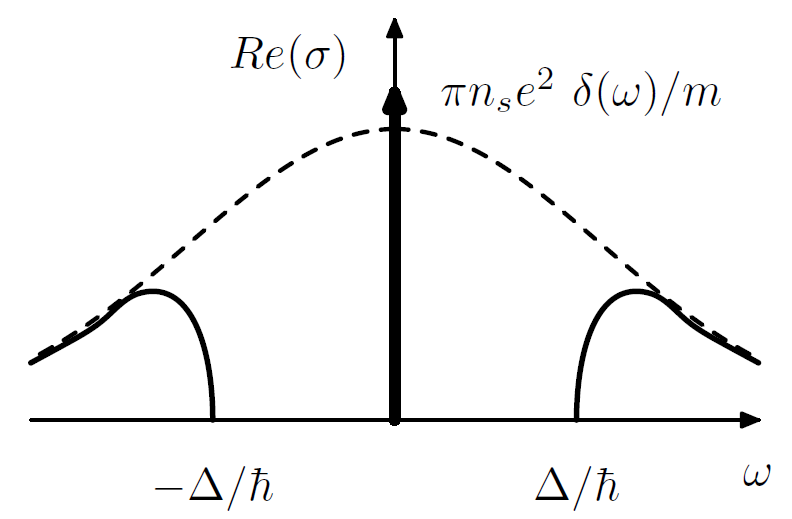
\includegraphics[width=.6\textwidth]{immagini/andamento_conducibilita.png}
   \caption*{Conducibilità a frequenza finita di un metallo normale (linea tratteggiata) e di un superconduttore (linea continua). Nel caso del superconduttore, un gap energetico porta a una conducibilità nulla per frequenze inferiori a $\Delta/\hbar$. Il peso spettrale rimanente si concentra in una funzione delta di Dirac in $\omega = 0$.}
\end{figure}
\hspace{-0.6cm}Tale comportamento conduttivo finito (che è simmetrico) somiglia molto a ciò che otterremmo dalla parte reale della conducibilità di un metallo normale. Infatti, possiamo vedere che coincide con la linea tratteggiata, che rappresenta il comportamento lorentziano tipico di un metallo normale. Oggi sappiamo che la frequenza in cui avviene questo cambiamento di comportamento corrisponde al gap superconduttivo, di cui abbiamo già parlato per un superconduttore.\\
Ciò significa che, se osserviamo la parte reale della conducibilità di un superconduttore, vediamo un picco a frequenza zero, seguito da una resistenza finita che compare a frequenze superiori a un certo valore caratteristico. Questo implica che, per frequenze superiori a tale valore, il sistema ha essenzialmente la stessa risposta di un metallo normale, per una ragione che, a questo punto, non possiamo ancora comprendere.\\
Supponiamo ora, seguendo questo ragionamento, di avere un materiale a resistenza zero, descritto da una conducibilità dipendente dalla frequenza come l'\eqrefcustom{eq:conduttivita_superconduttore} e andiamo a vedere quale forma ci si può aspettare per la densità di corrente. Quello che faremo sarà innanzitutto correlare questa densità di corrente $\vb{J}$ al potenziale vettore $\vb{A}$ (nel caso in cui venga applicato un campo magnetico, si noti che finora non è apparso alcun campo magnetico) e vedremo subito dopo che questa connessione tra $\vb{J}$ e $\vb{A}$ implica l'effetto Meissner.\\
Consideriamo l'\eqrefcustom{eq:legge_di_Ohm_in_sviluppo_di_Fourier} e calcoliamo il rotore di entrambi i membri:
\begin{equation*}
   \curl{\vb{J}} e^{-i\omega t}
   =\sigma(\omega) \curl{ \qty( \vb{E} e^{-i\omega t } ) }
\end{equation*}
Dalla legge di Faraday sappiamo che
\begin{equation*}
   \curl{\vb{E}}
   =-\pdv{\vb{B}}{t}
\end{equation*}
Possiamo sostituire nella precedente equazione, ottenendo
\begin{equation*}
   \curl{\vb{J}} e^{-i\omega t}
   =-\sigma(\omega) \pdv{t} \qty( \vb{B} e^{-i\omega t} )
   =i\omega \sigma(\omega) \vb{B} e^{-i\omega t}
\end{equation*}
Poiché stiamo considerando frequenze finite, la conducibilità ha solo la parte immaginaria\mn{Ricordiamo che ciò è dovuto alla presenza della $\delta(\omega)$, la quale implica che la parte reale è diversa da zero solo per frequenza nulla.}. Quindi l'equazione diventa
\begin{equation*}
   \curl{\vb{J}} e^{-i\omega t}
   =i\omega \qty( - \frac{n_s e^2}{i \omega m_e} ) \vb{B} e^{-i\omega t}
   =-\frac{n_s e^2}{m_e} \vb{B} e^{-i\omega t}
\end{equation*}
Prendiamo ora il limite per $\omega \to 0$, che significa considerare la risposta statica. Si ottiene
\begin{equation}
   \curl{\vb{J}}
   =-\frac{n_s e^2}{m_e} \vb{B}
   \label{eq:relazione_J_B}
\end{equation}
Sappiamo inoltre che il campo magnetico è in generale legato al potenziale vettore $\vb{A}$ tramite la relazione
\begin{equation}
   \vb{B}=\curl{\vb{A}}
   \label{eq:relazione_B_A}
\end{equation}
quindi possiamo riscrivere l'\eqrefcustom{eq:relazione_J_B} come
\begin{equation*}
   \curl{\vb{J}}
   =-\frac{n_s e^2}{m_e} \curl{\vb{A}}
\end{equation*}
Tuttavia, l'\eqrefcustom{eq:relazione_B_A} non identifica completamente il potenziale vettore in quanto essa è soddisfatta anche se aggiungiamo il gradiente di una funzione scalare $\chi$ ad $\vb{A}$. Per questa ragione, non possiamo immediatamente mettere in relazione $\vb{J}$ con $\vb{A}$, a meno di scegliere la gauge corretta per il potenziale vettore, che come abbiamo detto è la gauge di London. In conclusione, abbiamo che
\begin{equation*}
   \vb{J}
   =-\frac{n_s e^2}{m_e} \vb{A}
   \qq{se}
   \div{\vb{A}}=0
\end{equation*}
che è precisamente l'equazione di London che abbiamo dato in precedenza. Notiamo che la gauge di London è equivalente a considerare la condizione statica $\dv{\rho}{t}=0$.\\
In questo modo, abbiamo visto come, partendo dall'assunzione di avere un conduttore con resistività nulla, cioè un conduttore in cui una parte degli elettroni diventa superconduttiva, il che implica che la parte reale della conducibilità abbia la forma dell'\eqrefcustom{eq:conduttivita_superconduttore}, otteniamo una connessione tra la densità di corrente e il potenziale vettore.
\subsection{Spiegazione dell'effetto Meissner}
Vediamo ora come l'equazione di London sia in grado di prevedere l'effetto Meissner. Partiamo dalla legge di Ampere:
\begin{equation*}
   \curl{\vb{B}}
   =\mu_0 \vb{J}
\end{equation*}
Prendiamo il rotore di entrambi i membri:
\begin{equation*}
   \curl{(\curl{\vb{B}})}
   =\mu_0 \curl{\vb{J}}
\end{equation*}
Usando l'\eqrefcustom{eq:prima_equazione_di_London} e poi l'\eqrefcustom{eq:relazione_B_A}, possiamo scrivere:
\begin{equation*}
   \curl{(\curl{\vb{B}})}
   =-\mu_0 \frac{n_s e^2}{m_e} \curl{\vb{A}}
   =-\mu_0 \frac{n_s e^2}{m_e} \vb{B}
\end{equation*}
Notiamo che vale la relazione:
\begin{equation*}
   \curl{(\curl{\vb{B}})}
   =\grad{(\div{\vb{B}})} - \grad^2 \vb{B}
   =-\grad^2 \vb{B}
\end{equation*}
in quanto il campo magnetico è irrotazionale. Otteniamo quindi:
\begin{equation*}
   \grad^2 \vb{B}
   =\mu_0 \frac{n_s e^2}{m_e} \vb{B}
\end{equation*}
Se definiamo
\begin{equation}
   \lambda^2
   =\frac{m_e}{\mu_0 n_s e^2}
   \label{eq:lunghezza_di_penetrazione_London}
\end{equation}
che ha la dimensioni di una lunghezza al quadrato,\mn{Ci si può rendere conto che debba essere così per il fatto che a primo membro abbiamo l'operatore laplaciano, dunque affinché l'equazione sia consistente a livello dimensionale a destra dobbiamo avere l'inverso di una lunghezza al quadrato.} possiamo riscrivere
\begin{equation}
   \grad^2 \vb{B}
   =\frac{1}{\lambda^2} \vb{B}
   \label{eq:equazione_di_London_per_effetto_Meissner}
\end{equation}
L'\eqrefcustom{eq:equazione_di_London_per_effetto_Meissner} descrive precisamente l'effetto Meissner. Vediamolo esplicitamente in un caso semplice: supponiamo che lo spazio sia riempito da un superconduttore per $x>0$ e ci sia vuoto per $x<0$:
\begin{figure}[H]
   \centering
   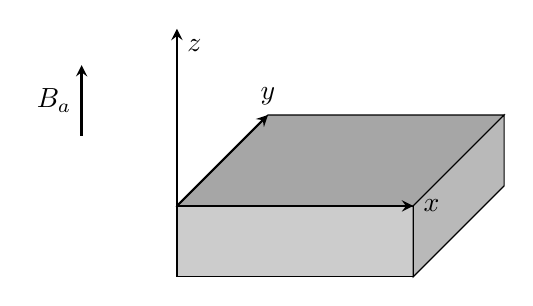
\begin{tikzpicture}[scale=1.5]
      %superconductor
      \draw[fill=gray!40] (0,0,0) -- (0,-.6,0) -- (2,-.6,0) -- (2,0,0) -- cycle;
      \draw[fill=gray!70] (0,0,0) -- (0,0,-2) -- (2,0,-2) -- (2,0,0) -- cycle;
      \draw[fill=gray!55] (2,0,0) -- (2,0,-2) -- (2,-.6,-2) -- (2,-.6,0) -- cycle;
      % Axes
      \draw[thick,-stealth] (0,0,0) -- (2,0,0) node[right] {$x$};
      \draw[thick,-stealth] (0,0,0) -- (0,1.5,0) node[anchor=north west] {$z$};
      \draw[thick,-stealth] (0,0,0) -- (0,0,-2) node[anchor=south] {$y$};
      % Campo magnetico
      \draw[thick,-stealth] (-1,.4,-.5) -- (-1,1,-.5) node[midway,left] {$\vb{B}_a$};
   \end{tikzpicture}
\end{figure}
\hspace{-0.6cm}Supponiamo di applicare nel vuoto un campo magnetico esterno $\vb{B}_a$ lungo la direzione $z$, ovvero $\vb{B}_a=B_z \vu{z}$, quindi parallelo alla superficie di contatto del superconduttore. Vediamo quale forma assume l'\eqrefcustom{eq:equazione_di_London_per_effetto_Meissner} in questa configurazione. Osserviamo innanzitutto che, poiché la componente parallela del campo magnetico non cambia attraversando l'interfaccia tra due mezzi, dovrà esserci un campo magnetico anche all'interno del superconduttore, diretto ancora lungo $z$.\\
Per prima cosa calcoliamo il termine $\grad^2 \vb{B}$:\mn{Per definizione, $\grad^2$ è dato dalla somma delle derivate seconde rispetto a $x$, $y$ e $z$ ma, considerando la simmetria del problema, non ci aspettiamo variazioni lungo le direzioni $y$ e $z$, mentre può esserci una variazione lungo $x$. Pertanto, l'operatore si riduce alla derivata seconda rispetto a $x$.}
\begin{equation*}
   \grad^2 \vb{B}
   = \grad^2 (B_z \vu{z})
   = \pdv[2]{B_z}{x} \vu{z}
\end{equation*}
Quindi, l'equazione di London per l'effetto Meissner diventa:
\begin{equation*}
   \pdv[2]{B_z}{x} \vu{z}
   =\frac{1}{\lambda^2} B_z \vu{z}
\end{equation*}
Ciò significa che la componente $z$ del campo magnetico deve soddisfare l'equazione
\begin{equation*}
   \pdv[2]{B_z}{x}
   =\frac{1}{\lambda^2} B_z
\end{equation*}
la cui soluzione è
\begin{equation}
   B_z(x)
   =B_z(0) e^{-x/\lambda}
   \label{eq:campo_magnetico_dentro_il_superconduttore}
\end{equation}
L'\eqrefcustom{eq:campo_magnetico_dentro_il_superconduttore} ci dice che, se osserviamo il profilo della componente $z$ del campo magnetico per $x>0$ ossia all'interno del superconduttore, vediamo che il campo magnetico parte da un valore finito in $x=0$, cioè esattamente sulla superficie, e poi decresce esponenzialmente all'interno del superconduttore su una lunghezza caratteristica pari proprio a $\lambda$.\\
\begin{marginfigure}
   \centering
   \begin{tikzpicture}
      \draw[->] (0,0) -- (4,0) node[right] {$x$};
      \draw[->] (0,0) -- (0,2.5) node[above] {$B_z(x)$};
      \draw[dashed] (1,0) node[below] {$\lambda$} -- (1,0.7357);
      \draw[thick,green!60!blue!] plot[domain=0:3.8,samples=100] (\x, {2*exp(-\x)});
   \end{tikzpicture}
   \caption*{Comportamento del campo magnetico all'interno di un superconduttore, in prossimità del bordo.}
\end{marginfigure}
\hspace{-0.35cm}Questo significa che, se abbiamo un superconduttore con questa particolare geometria immerso in un campo magnetico esterno (il campo applicato), all'interno del superconduttore non è presente campo magnetico. In altre parole, il campo che sarebbe presente se il materiale fosse normale viene espulso\sn{Notiamo che stiamo considerando la situazione finale: se potessimo osservare come si raggiunge questa condizione, vedremmo che raffreddando il superconduttore da temperature superiori alla temperatura critica a temperature inferiori ad essa, si passa da una situazione in cui il campo magnetico è uniforme in tutto lo spazio (compreso l'interno del metallo normale) a una in cui il campo viene praticamente espulso dal superconduttore, nel senso che solo una sottilissima regione sotto la superficie presenta ancora un campo magnetico finito, mentre il resto del materiale è caratterizzato da campo magnetico nullo.} e osserviamo che esso penetra soltanto in uno strato molto sottile sotto la superficie e, oltre una distanza dell'ordine di $\lambda$, il campo diventa praticamente nullo. Tale comportamento è esattamente quello che ci si aspetta dall'effetto Meissner.\\
Vediamo qual è il valore di $B_z(0)$. Come abbiamo detto, la componente parallela del campo magnetico non cambia attraversando una superficie, quindi il valore di $B_z$ in $x=0$ deve necessariamente essere uguale al campo applicato, quindi $B_z(0)=B_a$.\\
Possiamo osservare anche un altro aspetto. Descrivendo la fenomenologia di un superconduttore abbiamo detto che, se viene applicato un campo magnetico esterno, affinché il campo magnetico venga espulso deve esserci un'altra sorgente di campo magnetico che lo compensi esattamente. Abbiamo anticipato che ciò avviene perché sulla superficie del superconduttore si genera una supercorrente della quantità esattamente necessaria a generare un campo magnetico che compensi il campo applicato dall'esterno. Nella geometria dell'esempio che stiamo considerando, questo significa che, vicino alla superficie del materiale, esisterà un flusso di supercorrente tale da generare un campo magnetico opposto a $\vb{B}_a$. Ciò che faremo ora è calcolare la densità di corrente che scorre sulla superficie del superconduttore. Fare ciò è piuttosto semplice, perché abbiamo visto che esiste una relazione tra $\vb{J}$ e $\vb{A}$, o meglio tra $\curl{\vb{J}}$ e $\vb{B}$, data dall'\eqrefcustom{eq:relazione_J_B}. Poiché nel nostro caso il campo magnetico ha componente soltanto lungo $z$, possiamo considerare soltanto la componente $z$ del rotore di $\vb{J}$ e scrivere:
\begin{equation*}
   (\curl{\vb{J}})_z \vu{z}
   =-\frac{n_s e^2}{m_e} B_z \vb{z}
\end{equation*}
ovvero, esplicitando la componente del rotore,
\begin{equation*}
   \qty( \pdv{J_y}{x} - \pdv{J_x}{y} )
   =-\frac{n_s e^2}{m_e} B_z
\end{equation*}
Considerando la simmetria del problema, non ci aspettiamo una dipendenza da $y$ in quanto il sistema è simmetrico rispetto a tale direzione, quindi $\pdv{J_x}{y}=0$ e possiamo scrivere
\begin{equation*}
   \pdv{J_y}{x}
   =-\frac{n_s e^2}{m_e} B_a e^{-x/\lambda}
   =-\frac{\mu_0}{\lambda^2} B_a e^{-x/\lambda}
\end{equation*}
dove abbiamo esplicitato la forma del campo magnetico e poi utilizzato la definizione di $\lambda$ data dall'\eqrefcustom{eq:lunghezza_di_penetrazione_London}.\mn{Per ottenerla abbiamo moltiplicato e diviso per $\mu_0$.}\\
La soluzione di questa equazione è
\begin{equation*}
   J_y(x)
   =\frac{\mu_0}{\lambda} B_a e^{-x/\lambda}
\end{equation*}
In questo modo abbiamo dimostrato che esiste una densità di corrente, e quindi una supercorrente, che scorre lungo la direzione $y$, non nulla solo entro una regione di spessore $\lambda$ lungo la direzione $x$, cioè in uno strato del superconduttore parallelo al piano $xy$. Questa supercorrente genera un campo magnetico, diretto lungo $z$, che si può dimostrare essere tale da compensare esattamente il campo magnetico esterno applicato.
\subsection{Seconda coppia di equazioni di London}
A volte in letteratura, invece di trovare come definizione dell'equazione di London quella che abbiamo scritto nell'\eqrefcustom{eq:prima_equazione_di_London} associata alla gauge di London, si trova un'altra coppia di equazioni, che riguarda il rotore di $\vb{J}$ e la derivata temporale di $\vb{J}$. L'insieme di queste due relazioni è equivalente, come stiamo per dimostrare, all'\eqrefcustom{eq:prima_equazione_di_London} e alla gauge di London.\\
Consideriamo l'\eqrefcustom{eq:prima_equazione_di_London} e calcoliamo il rotore di entrambi i membri:
\begin{equation*}
   \curl{\vb{J}}
   =-\frac{n_s e^2}{m_e} \curl{\vb{A}}
\end{equation*}
Usando l'\eqrefcustom{eq:relazione_B_A}, possiamo scrivere
\begin{equation}
   \curl{\vb{J}}
   =-\frac{n_s e^2}{m_e} \vb{B}
   \label{eq:seconda_equazione_di_London}
\end{equation}
e l'\eqrefcustom{eq:seconda_equazione_di_London} è talvolta chiamata seconda equazione di London.\\
Prendiamo poi la derivata temporale dell'\eqrefcustom{eq:prima_equazione_di_London}:
\begin{equation*}
   \pdv{\vb{J}}{t}
   =-\frac{n_s e^2}{m_e} \pdv{\vb{A}}{t}
   %=-\frac{n_s e^2}{m_e} \vb{E}
\end{equation*}
Dall'elettromagnetismo sappiamo che, in generale, il campo elettrico può essere espresso come
\begin{equation*}
   \vb{E}=-\grad{\phi} - \pdv{\vb{A}}{t}
\end{equation*}
dove $\phi$ è il potenziale elettrico. Se $\phi$ è costante, possiamo scrivere
\begin{equation*}
   \pdv{\vb{J}}{t}
   =\frac{n_s e^2}{m_e} \vb{E}
   %=\frac{1}{\Lambda} \vb{E}
\end{equation*}
Se poniamo
\begin{equation*}
   \Lambda
   =\frac{m_e}{n_s e^2}
   %\label{eq:lunghezza_di_London}
\end{equation*}
possiamo scrivere
\begin{equation}
   \pdv{\vb{J}}{t}
   =\frac{1}{\Lambda} \vb{E}
   \label{eq:prima_equazione_di_London_alternativa}
\end{equation}
Talvolta, con prima equazione di London si intende l'\eqrefcustom{eq:prima_equazione_di_London_alternativa}.\\
Come possiamo vedere, l'\eqrefcustom{eq:seconda_equazione_di_London} e l'\eqrefcustom{eq:prima_equazione_di_London_alternativa} mettono in relazione la densità di corrente con il campo magnetico ed il campo elettrico, rispettivamente. C'è un punto importante da osservare: queste due equazioni non possono essere derivate l'una dall'altra. Infatti, non sono equivalenti, poiché forniscono due informazioni diverse sul superconduttore: una riguarda le proprietà di conduzione e l'altra riguarda le proprietà magnetiche, e come abbiamo già visto la conducibilità perfetta non implica l'effetto Meissner.\\
Ciò si può vedere partendo dall'\eqrefcustom{eq:prima_equazione_di_London_alternativa} e cercando di capire la risposta magnetica: se proviamo a farlo, vedremo che ciò non implica necessariamente l'effetto Meissner, che è una proprietà diversa. Per vedere tale fatto applichiamo il rotore all'\eqrefcustom{eq:prima_equazione_di_London_alternativa}:
\begin{equation*}
   \curl{\pdv{\vb{J}}{t}}
   =\frac{1}{\Lambda} \curl{\vb{E}}
   =-\frac{1}{\Lambda} \pdv{\vb{B}}{t}
\end{equation*}
dove nell'ultimo passaggio abbiamo usato la legge di Faraday. Portando tutto al primo membro otteniamo
\begin{equation*}
   \curl{\pdv{\vb{J}}{t}} + \frac{1}{\Lambda} \pdv{\vb{B}}{t}=0
\end{equation*}
Supponendo di poter scambiare l'ordine di derivazione rispetto al tempo e allo spazio, possiamo scrivere
\begin{equation*}
   \pdv{t} \qty( \curl{\vb{J}} ) + \frac{1}{\Lambda} \pdv{\vb{B}}{t}=0
\end{equation*}
e raccogliendo i due termini otteniamo
\begin{equation*}
   \pdv{t} \qty( \curl{\vb{J}} + \frac{1}{\Lambda} \vb{B} )=0
\end{equation*}
Confrontiamo tale relazione con l'\eqrefcustom{eq:seconda_equazione_di_London}: la prima ci dice che la quantità tra parentesi è costante ma non necessariamente nulla, mentre la seconda ci dice che è proprio nulla. Questo significa che la prima equazione di London, che descrive direttamente la risposta di una supercorrente a un campo elettrico, non è in grado di descrivere la risposta di un superconduttore a un campo magnetico, e in particolare l'effetto Meissner. Ne segue che, per mettere in relazione $\vb{J}$ sia con il campo elettrico che con il campo magnetico, sono necessarie sia la prima che la seconda equazione di London oppure, in alternativa, l'equazione di London che collega $\vb{J}$ al potenziale vettore $\vb{A}$ insieme alla gauge di London.\\
Derivation of \eqrefcustom{eq:prima_equazione_di_London_alternativa} for a perfect conductor is very intuitive if we use again a drude type description of the of the conductor. We know that Ohm's law can be derived if we consider the average response of the electrons in the presence of an external applied electric field:
\begin{equation}
   m_e \dv{\vb{v}}{t}
   =-e \vb{E} - \frac{m_e}{\tau} \vb{v}
   \label{eq:modello_di_Drude}
\end{equation}
This equation comes by considering the average motion of an electron to an applied electric field, including a viscous force describing the effect of the collisions which electrons suffer while moving in the conductor. If we consider in this regime the superconductor as a perfect conductor, meaning, as we said, that $\tau \to \infty$, it means that we have to neglect the damping term due to collisions, so \eqrefcustom{eq:modello_di_Drude} can be written as
\begin{equation*}
   -e n_s \dv{\vb{v}}{t}
   =\frac{e^2 n_s}{m_e} \vb{E}
\end{equation*}
where we have multiplied both members by $-\frac{e n_s}{m_e}$. We notice that the left hand side is just the derivative with respect to time of the current density $\vb{J}$, while in the right hand side we can recognize that the coefficient is equal to $1/\Lambda$, so this is precisely \eqrefcustom{eq:prima_equazione_di_London_alternativa}, that is the first London equation. So this is an equivalent way of deriving the two sets of the phenomenological London equations.\\
\subsection{La lunghezza di penetrazione di London}
\textbf{Nota: questa parte è da sistemare.}\\
Concentriamoci ora sulla previsione che possiamo ottenere dalla lunghezza di penetrazione di London. L'ordine di grandezza di $\lambda$ dipende dal materiale considerato. Come abbiamo visto, $\lambda$ è definita dall'\eqrefcustom{eq:lunghezza_di_penetrazione_London} e dipende da alcune quantità note con precisione e dalla densità degli elettroni superconduttivi $n_s$, che invece non conosciamo. Possiamo tuttavia stimare quest'ultima: poiché abbiamo assunto che la densità totale di elettroni in un superconduttore sia data dall'\eqrefcustom{eq:densita_elettroni}, possiamo ipotizzare che, nello stato superconduttivo, la frazione di elettroni normali sia trascurabile rispetto a quella degli elettroni superconduttivi.\\
Se questa ipotesi è valida, possiamo stimare che $n_s$ sia approssimativamente uguale alla densità totale di elettroni $n$. Quest'ultima deve coincidere con la densità elettronica del materiale nello stato normale, poiché, secondo il modello considerato, nel passaggio alla fase normale la densità di elettroni superconduttivi si annulla, lasciando invariata la densità totale di elettroni, che è quindi quella tipica del metallo normale, dell'ordine di $10^{22} \; \rm cm^{-3}$. Sulla base di questa stima, possiamo calcolare la lunghezza di penetrazione, che risulta, in queste condizioni, dell'ordine di 100 \A.\\
In realtà, gli esperimenti mostrano che $\lambda$ dipende dalla temperatura. Ciò significa che, ricavando da $\lambda(T)$ la corrispondente densità sperimentale $n_s(T)$, otteniamo una certa relazione funzionale. In particolare, si osserva che la dipendenza di $\lambda$ dalla temperatura segue una legge di potenza, che può essere espressa come:
\begin{equation*}
   \lambda(T)
   =\frac{\lambda(0)}{\sqrt{ 1 - \qty(\frac{T}{T_c})^{4}}}
\end{equation*}
Assumendo che a temperatura nulla tutti gli elettroni diventino superconduttivi, $\lambda(0)$ risulta proporzionale alla densità elettronica. Tuttavia, i dati sperimentali mostrano in genere che $\lambda(0)$ ha un valore dell'ordine di 500 \A, quindi maggiore rispetto alla stima teorica precedente.\\
%Let's now focus on the prediction we have from the London penetration depth. The order of magnitude of $\lambda$ depends on the material. As we have seen, $\lambda$ is defined by \eqrefcustom{eq:lunghezza_di_penetrazione_London} and it depends on some quantities we precisely know and on the density of superconductive electrons $n_s$, which we don't know. However, we can make an estimate: since our initial assumption is that the overall density of electrons in the superconductor is given by \eqrefcustom{eq:densita_elettroni}, we can assume that when the material is superconductive, the fraction of normal electrons is negligible with respect to the fraction of superconductive electrons. If this is the case, and this is an assumption, we can estimate that $n_s$ is almost equal to the density of electrons $n$, which must be the same as the density of electrons we have when the system becomes a normal metal because in the other regime, according to this model, the superconductive electrons density vanishes for some mysterious reason and the overall density of electrons is the one of the normal metal, which is a quantity we know and which is of the order to $\rm 10^{22}/cm^3$. So, according to this estimate, we can evaluate the penetration depth, which turns out to be, with this assumption, of the order of 100 \A.\\
%Actually, what we see from experiments is that $\lambda$ depends on temperature, so this means that if we extrapolate from the experimental $\lambda(T)$ an experimental $n_s(T)$ we will get some form. In particular, we find that $\lambda$ depends on temperature with the power law, which can be extrapolated to be

%So, assuming that at zero temperature all electrons becomes superconducting, then in this case $\lambda(0)$ is proportional to the density of electrons. Actually, experiments tipically give for $\lambda(0)$, a quantity which in general is the order of $500 \A$, so they give a larger value.
%%
This larger penetration depth can be predicted by refining the model, and the way this model is refined is similarly to what is done for a normal conductor, where instead of describing its response in terms of the Drude model, leading to the Ohm's law, we describe the non-local response of a normal metal which will bring a non-local response also for a superconductor.\\
\textbf{c'è una parte commentata da sistemare qui sotto}\\
%Qualitatively what we will do is the following: so far, we considered, with the Drude model, a local response, which means that if we are in a metal and we have an electric field in one point, precisely at the same point we will have a current density $\vb{J}$, which is given by $\vb{J}=\sigma\vb{E}$. Non local response means that the current density we will have in some point is not depending only on the electric field at the same point, but it depends on the electric field in some area, with some length scale, which depends on this area, which is depending on how we describe it. The result is that we have a question. Do you expect this J-prime to be larger or smaller than J? Depending on the field Well, if it depends on the field, if the field contributes to the area, we mean, it agrees with the local contribution, but it's bigger. J was in my opinion. we don't know. I'm very close to the final time. No, not in the same sense. Did this J What would it be like this? What does this mean? That t
%The fact that current density depends on the behavior of the electric field in some area around the point means that we have a sort of average effect on the electrons in one point, coming from how the field is in that area, and tipically what happens is that there is a sort of screening, because in the material we don't have only the electric field but we have also electrons and other stuff. So in practice, the response is smaller than $\vb{J}$. Now let's try to think through an analogous behavior where we have a superconductor. If we consider it as a non-local field, we have a response, meaning a superconductor current density, which is smaller than the supercurrent density we would obtain in the other case. What should we expect as a magnetic field? What does the magnetic field the magnetic field in the part which is still not so big within some length scale? we have a smaller supercurrent. The magnetic field generated by the superconductor to oppose the applied one is smaller. Therefore, the field is not damaged in the larger So we have a smaller supercurrent and a smaller screen of the external and the magnetic field does it extends in the larger space. This is the Perfect. Let's think about it. Why do we build and change things?

%, this again. And it has a special temperature depending on it. Now, the point is that this is a sort of Let's say, sort of phenomenological description. But the point is that also in theory, it was possible to release some of the assumptions we have done. And it turned out that it is possible to make a phenomenological model which is a little bit more accurate, the one which we have done now coming basically from the Drude model and this more accurate model, still classical, is what we call the Porter model. No, the Porter model is another one still. But physically, independently on the right, physically, the idea is that the Ruder model considers a non local response of electrons to an applied magnetic field. So, electric field. The Ruder model tells us, Ruder model says that, we have an electric field, we will have a $\vb{J}$, which is $\sigma \vb{E}$, and it is the same everywhere. So, if we apply electric field here, like this, we will have a current here, the current density here, which is not Already at the classical level, this is not . And it is impossible actually to make a little bit more sophisticated model, which considers the no-locker response of electrons. So, meaning that if we have the same in general, if we do not have a field which is uniform, in particular, we have to remove the surface. And the issue is that the response, so J, is not depending entirely on E in the same place, but on the integral over the volume, told in the letter to use here. Of some, let me call it a function of the energy. So, this is just to say that it was possible that this will be a topic of final lecture. final lecture. On final lecture, we will see that in order to get an address of that which is larger, which is closer to what experiments tell us at any time, it is needed to make a little bit more sophisticated theory of transport, which is not the new model, which is no-locker, but which is based on the local response of electrons to the electric field. This will give us also, meaning this pathological approach, a more realistic expression from the very address, which is quantitatively closer to the real experiment. This is a prediction of what happens. What we can do now is just extrapolate the value of the test, doesn't tell us anything about what is going on. That's the source of the test result.

\section{Modello di Pippard}
Abbiamo visto che la previsione che facciamo con la teoria di London, una volta confrontata con i risultati sperimentali che danno la dipendenza dalla temperatura, ci dà un valore estrapolato a temperatura nulla che è quello che otteniamo con l'espressione di London che possiamo stimare con la densità degli elettroni data da quelli degli elettroni normali e ci dà un valore più piccolo di quello che nella maggior parte dei metalli allo stato puro si misura. L'idea che allora venne in mente è che, se c'è una penetrazione maggiore del campo magnetico, vuol dire che c'è un minore schermaggio, quindi si stabilisce una corrente superconduttiva più bassa. L'idea fu che potesse essere attribuibile ad una risposta non locale del superconduttore al campo magnetico applicato. Il fatto di avere una risposta non locale in un metallo in generale non è una cosa inusuale: anche la teoria classica della conduzione dei metalli prevede una teoria non locale che è più accurata del modello di Drude che utilizziamo di solito, che invece ci dà una risposta locale, cioè il campo elettrico in un punto ha un certo valore e la densità di corrente in quel punto è proporzionale al campo stesso tramite la connucibilità. Questo risultato viene fuori dal modello di Drude nell'ipotesi che il campo campo sia uniforme in tutti i punti del metallo. Se così non è, come di fatto avviene nella maggior parte dei casi, bisogna adoperare una teoria un po' più sofisticata anche per il problema della conduzione dei metalli. Questa teoria è quella che fu sviluppata e che porta alla legge di Chamber.
\subsection{Legge di Chamber}
Supponiamo di avere un sistema e di voler vedere la risposta, cioè la densità di corrente in un punto $\vb{r}$. Se abbiamo un campo elettrico che varia in una regione di spazio che è dell'ordine del libero cammino medio $l$ di un elettrone all'interno del conduttore, in realtà dobbiamo considerare l'effetto del campo elettrico in questa regione di spazio, è quindi una sorta di effetto medio di questo campo elettrico in questa regione di spazio e questo effetto medio è descritto dalla seguente legge:\mn{In questo corso non ricaviamo tale legge, ci limiteremo soltanto a commentarla.}
\begin{equation}
   \vb{J}(\vb{r})
   =\frac{3\sigma}{4\pi l} \int \frac{\vb{R} \qty[ \vb{R} \vdot \vb{E}(\vb{r}') ] }{R^4} e^{-R/l} \dd[3]{\vb{r}'}
   \label{eq:legge_di_Chamber}
\end{equation}
dove $R=\vb{r} - \vb{r}'$.\\
Essa ci dà una risposta che è proporzionale alla conducibilità e ad un integrale su un volume centrato intorno al punto nel quale stiamo cercando la risposta, la quale risente dell'effetto del campo elettrico  in una regione di spazio delle dimensioni dell'ordine di $l$. Questo lo vediamo nel fatto che abbiamo una scala $R$, cioè una distanza rispetto al libero cammino medio e l'espressione che si ricava da questo modello più dettagliato ci dice che l'effetto che abbiamo è più piccolo ed è essenzialmente legato al fatto che abbiamo all'interno un esponenziale che ci permette di dire che la risposta è ridotta. Ricavare questa espressione significa risolvere l'equazione di Boltzmann del trasporto per un processo in cui ci sono processi di scattering di elettroni, con una scala che è quella del libero cammino medio.\\
Prima di passare al superconduttore, c'è un passaggio intermedio che nasce da un'intunizione di Pippard che intuì che il meccanismo alla base della superconduttività non potesse essere un meccanismo descritto dalla fisica classica ma che ci dovesse essere una descrizione quantistica del comportamento di elettroni e in quel caso la cosa più ovvia da immaginare è che per qualche motivo la conduzione con quelle caratteristiche fosse legata a un trasporto di carica descritto in termini di una funzione d'onda. Quindi, anche senza precisare quale fosse la carica dei portatori di corrente in quel caso, l'idea è che abbiamo delle particelle elementari che per qualche motivo vanno descritte in maniera quantistica, quindi con un pacchetto d'onda, e per un pacchetto d'onda possiamo associare una larghezza legata all'indeterminazione nella quantità di moto delle particelle descritte da questo pacchetto (ricordiamo che c'è un principio di indeterminazione che lega l'indeterminazione di queste due variabili coniugate).\\
L'intuizione di Pippard sta nel fatto che egli osservò che vediamo manifestarsi il fenomeno della superconductività al di sotto di una certa temperatura che è la temperatura critica, e possiamo associare alla temperatura critica una scala di energia che è l'energia termica a quella temperatura. Inoltre gli elettroni coinvolti nel moto possiamo descriverli introducendo la velocità di Fermi $v_F$. Con queste quantità possiamo stimare un'indeterminazione nella quantità di moto degli elettroni semplicemente facendo il rapporto tra l'energia associata alla temperatura alla quale questo fenomeno si manifesta e la velocità degli elettroni che presumibilmente sono quelli che partecipano a questo fenomeno:
\begin{equation*}
   \Delta p
   \sim \frac{K_B T_c}{v_F}
\end{equation*}
In questo modo otteniamo una scala che ha le dimensioni di un momento. Se assumiamo che questa sia l'indeterminazione delle particelle che sono alla base del fenomeno superconductivo, l'indeterminazione che abbiamo in corrispondenza sulla posizione sarà
\begin{equation*}
   \Delta x
   \geq \frac{\hbar v_F}{K_B T_c}
\end{equation*}
Tale relazione ci dà una nuova scala di lunghezza che è quantistica (in quanto è presente il fattore $\hbar$) e comprende le caratteristiche del fenomeno superconduttivo perché è legata alla temperatura critica. Questa scala di lunghezza viene chiamata lunghezza di coerenza di Pippard, che si definisce come
\begin{equation*}
   \xi_0^{(\text{P})}
   =a \frac{\hbar v_F}{K_B T_c}
\end{equation*}
dove $a$ è un prefattore.\\
Supponiamo quindi che ci sia questa nuova scala di lunghezza che entra in gioco quando abbiamo il superconduttore, allora consideriamo questa scala come una scala che interviene nella definizione della lunghezza che ci dà la scala nella quale dobbiam valutare l'effetto medio, non di un campo elettrico perché stiamo parlando di un superconduttore, ma dell'analoga relazione che lega la densità di supercorrente al potenziale vettore perché la legge che descrive il comportamento della supercorrente è la legge di London. Quindi l'idea è quella di modificare la legge di London in maniera analoga a come la legge di Chamber modifica la legge di Ohm e la scala di lunghezza che io consideriamo al posto del libero cammino medio è una scala che tiene conto di questo fenomeno e che quindi tiene conto in questo modello di questa lunghezza. L'idea di Pippard, che fu colui che ideò questo modello nel 1953, fu quella di generalizzare l'equazione di London in maniera non locale nel seguente modo:
\begin{equation}
   \vb{J}_s(\vb{r})
   =-\frac{n_s e^2}{m_e} \frac{3}{4\pi \xi_0} \int \frac{\vb{R} \qty[ \vb{R} \vdot \vb{A}(\vb{r}') ] }{R^4} e^{-R/r_0} \dd[3]{\vb{r}'}
   \label{eq:modello_di_Pippard}
\end{equation}
Il termine $-\frac{n_s e^2}{m_e}$ ed il potenziale vettore erano già presenti nell'equazione di London, però abbiamo modificato l'equazione con una struttura identica a quella della legge di Chamber. Notiamo che nel fattore esponenziale, che è quello che ci dà un effetto di schermaggio, dobbiamo considerare una scala di lunghezza $r_0$ che tenga conto del fatto che in certi casi possiamo avere la risposta locale che va bene, in certi casi no. Per tale motivo, in questa scala di lunghezza efficace Pippard considerò sia la lunghezza del libero cammino medio che la lunghezza di coerenza, infatti $r_0$ è definita in maniera tale che
\begin{equation*}
   \frac{1}{r_0}
   =\frac{1}{l} + \frac{1}{\xi_0}
\end{equation*}
Nel seguito vedremo in che maniera questa formula ci permette di andare da un regime di risposta locale a uno di risposta non locale a seconda del peso relativo di queste due grandezze. Prima di fare questo però osserviamo una cosa che in qualche maniera ci permette anche di giustificare questa teoria fenomenologica a posteriori sulla base delle previsioni della teoria BCS. La teoria BCS introduce in maniera rigorosa, quella che si chiama lunghezza di coerenza BCS che è data da
\begin{equation*}
   \xi_0^{(\text{BCS})}
   =\frac{\hbar v_F}{\Delta}
\end{equation*}
dove $\Delta$ è la gap superconduttiva, la quale abbiamo già visto essere dell'ordine di $K_B T_C$, quindi in realtà tale lunghezza, a parte un pretattore, non è molto diversa dall'espressione che su base di plausibilità introduse Pippard. Nella teoria BCS questa lunghezza di correlazione ha un significato fisico molto preciso perché è una teoria microscopica e rappresenta una lunghezza di correlazione tra i due elettroni che formano le cosiddeette coppie di Cooper che sono all'origine della supercorrente in un superconduttore. In altre parole, la corrente superconduttiva nasce dalla formazione di coppie di Cooper, cioè due elettroni con caratteristiche di momento e spin opportune che formano un unico "oggetto" e essendo due particelle possiamo definire una lunghezza di correlazione che ci dà un'idea dell'estensione della funzione d'onda di due particelle che descrive la coppia di Cooper. In maniera approssimativa, possiamo dire che rappresenta la dimensione della coppia di Cooper, però va intesa in senso di lunghezza di correlazione in una descrizione più preciso. Il motivo per cui abbiamo fatto questo inciso è per dire che questa lunghezza di Pippard, introdotta in maniera qualitativa, semi-femomenologica, ha una sua giustificazione nella teoria mbicroscopica che seguì dopo.\\
Detto ciò, vediamo a questo punto come questa espressione ci permetta da una parte di avere una risposta con una lunghezza di penetrazione maggiore rispetto a quella prevista dalla teoria locale, e d'altra parte, vediamo come questa equazione possa riportarsi alla teoria locale sotto opportune condizioni.\\
Vediamo innanzitutto cosa cosa ci dice l'\eqrefcustom{eq:modello_di_Pippard}. Supponiamo di avere un campo magnetico che non sia uniforme sulla scala di $r_0$, in tal caso tale equazione in generale ci darà una densità di corrente che è più piccola di quella data dall'equazione di London, in cui abbiamo semplicemente il potenziale vettore nel punto in cui abbiamo la corrente. Questo fatto, come abbiamo detto già varie volte, fa sì che ci sia una supercorrente più piccola e quindi uno screening inferiore e una maggiora lunghezza di penetrazione. Tale situazione si ha in tutti i casi in cui il libero cammino medio del metallo, è molto più piccolo della lunghezza di coerenza, cioè quando $\xi_0 \gg l$.\sn{Aggiunta di chatGPT:\\
In questo caso infatti, la scala di lunghezza efficace $r_0$ è praticamente uguale a $l$, perché in questo caso $\frac{1}{l} \gg \frac{1}{\xi_0}$ e quindi $r_0 \sim l$. In questo caso, se il campo magnetico varia su una scala di lunghezza dell'ordine di $l$, che è molto più piccola della lunghezza di coerenza, allora siamo nel regime in cui la risposta non è locale e quindi abbiamo una lunghezza di penetrazione maggiore.}. Ad esempio, nell'alluminio il libero cammino medio a temperatura ambiente è dell'ordine di $200 \; \A$, mentre la lunghezza di correlazione di Pippard, facendo una stima basata sulla velocità di Fermi e sulla temperatura critica è dell'ordine di $10^4 \; \A$, quindi siamo nel regime in cui il libero cammino medio è molto più piccolo di $\xi_0$, quindi $\frac{1}{l} \gg \frac{1}{\xi_0}$ e quindi la densità di corrente supercondultiva sarà ridotta.\\
Il regime opposto, quindi il regime della teoria locale ce l'abbiamo invece quando abbiamo un potenziale vettore che è uniforme su scale di lunghezza dell'ordine di $\xi_0$ nel regime in cui il libero cammino medio è molto più grande di $\xi_0$, perché in questo caso avremo che $\frac{1}{l} \ll \frac{1}{\xi_0}$, quindi $r_0 \sim \xi_0$ e se $\vb{A}$ è uniforme su una scala di lunghezza dell'ordine di $\xi_0$ lo possiamo portare fuori dall'integrale e ci riconduciamo a un'espressione che si  riduce alla teoria locale. Possiamo quindi dire che questa generalizzazione non locale ci permette di recuperare la teoria locale nel momento in cui abbiamo un libero cammino medio sufficientemente grande, mentre quando abbiamo un libero cammino medio non abbastanza grande e un campo magnetico che varia ci dà una risposta ridotta.\\
Osserviamo che abbiamo introdotto tre scale di lunghezza: il libero cammino medio $l$, la lunghezza di coerenza di Pippard $\xi_0$ e la lunghezza di penetrazione $\lambda$. In particolare, $l$ e $\xi_0$ ci dicono se vale l'espressione locale o quella non locale, e questi due regimi vedono anche classificanti come
\begin{itemize}
   \item \textit{Regime clean}: quando $l \gg \xi_0^{(\text{P})}$
   \item \textit{Regime dirty}: quando $l \ll \xi_0^{(\text{P})}$
\end{itemize}
Il regime dirty è anche quello che si ha nelle leghe  che mostrano un comportamento superconduttivo nonostante abbiano una struttura altamente disordinata rispetto a quella dei metalli allo stato puro.
\subsection{Superconduttori del primo e del secondo tipo}
La relazione tra la lunghezza di penetrazione e la lunghezza di coerenza ci permette invece di destinguere due tipi di superconduttore. Tale fatto viene introdotto con precisione nella teoria di Ginzburg--Landau, ma possiamo fare già adesso questa distinzione perché vediamo come questa questa diversa relazione ci permette anche di spiegare la fenomenologia dei superconduttori del primo e del secondo tipo. Infatti noi fino ad ora abbiamo studiato i superconduttori del primo tipo anche se non li abbiamo chiamati così.
\begin{figure}[H]
   \centering
   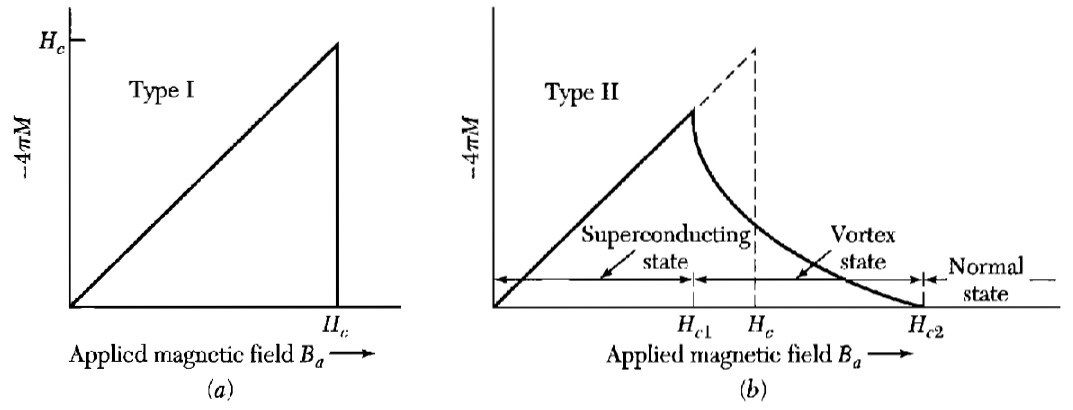
\includegraphics[width=\textwidth]{immagini/superconduttori_tipo_1_e_2.png}
   \caption*{Andamento della magnetizzazione in funzione del campo magnetico applicato per superconduttori del primo tipo (a) e del secondo tipo (b).}
\end{figure}
\hspace{-0.6cm}I materiali superconduttori del primo tipo sono quelli nei quali la lunghezza di penetrazione è più piccola della lunghezza di coerenza, viceversa nel regime opposto abbiamo i superconduttori del secondo tipo. I due tipi di superconduttori hanno una fenomenologia diversa\sn{Il fatto che si abbia una fenomenologia diversa, che stiamo per descrivere, sarà giustificato dalla teoria di Ginzburg--Landau, la quale studia situazioni in cui c'è un campo magnetico che ha una variazione nello spazio, a differenza delle teorie fenomenologiche precedenti che non hanno granché considerato la diversa risposta in queste condizioni. Essa ci permetterà di capire come tale fenomenologia nasca da essenzialmente considerazioni energetiche, cioè da come sia più conveniente da un punto di vista energetico per il materiale superconduttivo avere una penetrazione del campo magnetico con certe strutture oppure con altre.}, che è la seguente: finora abbiamo considerato superconduttori del primo tipo, che sono quelli nei quali al di sotto della temperatura critica abbiamo una risposta a un campo magnetico che è descritta dall'effetto Meissner, ovvero da un diamagnetismo perfetto, cioè se abbiamo un campo applicato $\vb{H}$, fino al valore $H_c$ abbiamo una magnetizzazione che è legata al campo applicato dalla relazione che si ha nel caso della risposta perfettamente diamagnetica, quindi abbiamo una separazione tra le due fasi con un unico valore del campo critico. I superconduttori del secondo tipo invece hanno un "diagramma di fase" un po' più articolato, nel senso che in questo caso abbiamo due valori del campo critico: un primo valore $H_{c,1}$ al di sotto del quale in effetti c'è la risposta diamagnetica con il perfetto diamagnetismo, dopo di che, superato il valore $H_{c,1}$, non si ha una risposta perfettamente diamagnetica ma non si ha nemmeno un passaggio immediato ad un comportamento normale, cioè c'è una regione di spazio in cui la relazione tra la magnetizzazione del campo critico è quella mostrata nel grafico di sopra. Nel momento in cui il sistema raggiunge un secondo valore di campo critico $H_{c,2}$, si ha il passaggio allo stato di metallo normale. In questa ragione tra i due valori di campo critico non abbiamo una perfetta espulsione del campo magnetico come abbiamo invece al di sotto di $H_{c,1}$, ma abbiamo una penetrazione del campo magnetico secondo una struttura particolare che è quella descritta da stati di vortice. Tale fatto lo possiamo vedere rappresentato qualitativamente nel seguente diagramma in funzione della temperatura e del campo magnetico:
\begin{figure}[H]
   \centering
   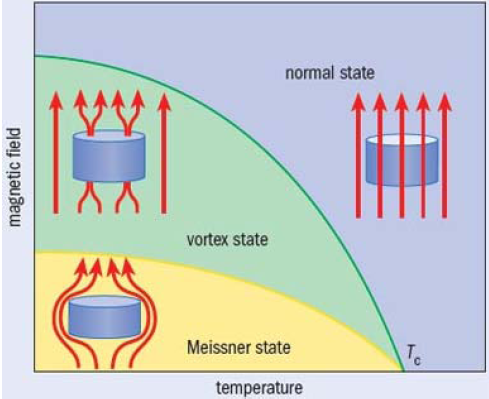
\includegraphics[width=0.6\textwidth]{immagini/grafico_T_H_superconduttori_tipo_2.png}
\end{figure}
\hspace{-0.6cm}Nel caso dei superconduttori del secondo tipo abbiamo una fase in cui abbiamo il comportamento perfettamente diamagnetico, quindi con la perfetta espulsione del campo magnetico dal materiale, una fase normale in cui invece il campo magnetico entra completamente nel materiale al di sopra della temperatura critica e una fase detta stato di vortice in cui il materiale è ancora superconductivo ma ci sono delle regioni all'interno del materiale che diventano normali le quali hanno una struttura che vede la penetrazione del campo magnetico sotto forma di vortici. Quello che cioè vedremo sono delle linee di campo magnetico che attraversano il materiale superconduttivo e a queste linee di campo magnetico che penetrano il materiale si associa una supercorrente intorno alla regione normale sotto forma di vortice, quindi una corrente che circola come se fosse intorno alla superficie di un cilindro che ha struttura\sn{credo intenda fase normale} normale. Viceversa nel regime di Meissner quello che abbiamo visto è che abbiamo una supercorrente solamente sulla superficie del materiale per una regione pari alla lunghezza di penetrazione.\sn{Man mano che il campo magnetico aumenta arrivando al campo magnetico critico quello che succede è che questa struttura di vortici diventa via via sempre più fitta fino a quando il campo magnetico penetra completamente nel materiale raggiungendo quindi lo stato normale.}
\subsection{Vortici di London}
Cerchiamo di capire più precisamente come sono fatti questi vortici. Questi in realtà possono essere già previsti dalla teoria di London e nel seguito vedremo come.\\
L'idea è rappresentata nella seguente figura:
\begin{figure}[H]
   \centering
   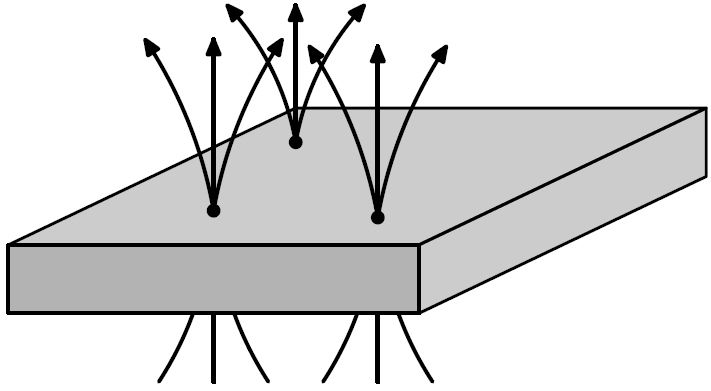
\includegraphics[width=0.5\textwidth]{immagini/vortici di London.png}
\end{figure}
\hspace{-0.6cm}Abbiamo il campo magnetico che entra all'interno del superconduttore formando un piccolo "vortex core" (in italiano "nucleo vortice") che si trova nello stato normale, quindi la regione in cui il campo magnetico penetra è una regione normale. Cerchiamo allora di capire cosa abbiamo:
\begin{figure}[H]
   \centering
   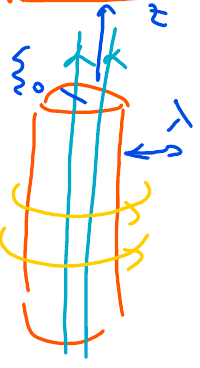
\includegraphics[width=0.2\textwidth]{immagini/vortex_core.png}
\end{figure}
\hspace{-0.6cm}Abbiamo una regione, che rappresentiamo con forma cilindrica, attraversata dal campo magnetico e il cui raggio è dell'ordine della lunghezza di coerenza. Per distanze dall'asse maggiori di $\xi_0$ ma più piccole di $\lambda$ abbiamo praticamente un superconduttore e quindi una densità di corrente $\vb{J}$ e avremo un certo campo magnetico $\vb{B}$. Possiamo ricavare questi due dall'equazione di London, la quale abbiamo visto si trasforma in un'equazione per il campo magnetico che è l'\eqrefcustom{eq:equazione_di_London_per_effetto_Meissner}, la quale, applicata ad un problema con geometria cilindrica come in questo caso e immaginando di avere un campo magnetico che è diretto lungo l'asse $z$, diventa
\begin{equation*}
   \dv[2]{B_z}{r} + \frac{1}{r} \dv{B_z}{r} - \frac{1}{\lambda^2} B_z
   =0
\end{equation*}
Tale equazione ha una soluzione nota che è espressa in termini della funzione di Bessel di ordine zero e che ha la seguente espressione:
\begin{equation*}
   B_z(r)
   =\frac{\Phi_0}{2\pi \lambda^2} K_0\qty(\frac{r}{\lambda})
\end{equation*}
dove $r$ è la distanza dall'asse e il coefficiente di proporzionalità è il flusso del campo magnetico attraverso una superficie che corrisponde alla sezione della regione normale. Quello vogliamo fare adesso a partire da questa espressione è vedere che forma assume il campo magnetico all'interno della regione di lunghezza $\lambda$ e vogliamo anche vedere com'è fatta la supercorrente. Prima di tutto consideriamo l'andamento della funzione di Bessel $K_0$, la quale quando ha argomento molto più piccolo di uno può essere approssimata nella seguente maniera:
\begin{equation*}
   K_0(z)
   \sim -\ln(z)
   \qq{se} z \ll 1
\end{equation*}
Nel nostro problema la condizione sull'argomento, visto che l'argomento di $K_0$ è $r/\lambda$, equivale a dire che $r \ll \lambda$ (ma chiaramente si deve avere comunque $r>\xi_0$, perché stiamo guardando l'equazione di London nella regione in cui il materiale è superconduttivo). In tale regione possiamo quindi riscrivere l'equazione di London come
\begin{equation}
   B_z(r)
   \sim \frac{\Phi_0}{2\pi \lambda^2} \ln\qty(\frac{\lambda}{r})
   \qq{se} \xi_0 < r \ll \lambda
   \label{eq:campo_magnetico_vortex_interno}
\end{equation}
dove abbiamo usato la proprietà del logaritmo $-\ln(z)=\ln\qty(\frac{1}{z})$.\\
Viceversa, la funzione di Bessel per argomento molto maggiore può essere approssimata come
\begin{equation*}
   K_0(z)
   \sim \sqrt{\frac{\pi}{2z}} e^{-z}
   \qq{se} z \gg 1
\end{equation*}
per cui l'equazione di London diventa
\begin{equation*}
   B_z(r)
   \sim \frac{\Phi_0}{2\pi \lambda^2} \sqrt{\frac{\pi \lambda}{2r}} e^{-r/\lambda}
   \qq{se} r \gg \lambda
\end{equation*}
La soluzione per $r \gg \lambda$ ci dà un andamento abbastanza simile, sebbene un po' più smorzato, a quello che avremmo nel caso del superconduttore di primo tipo.\\
Rivolgiamo di nuovo la nostra attenzione alla regione per valori di $r<\lambda$. In tale regione il campo magnetico ci dà una corrente che vogliamo ricavare. Per fare ciò applichiamo la legge di Ampere:
\begin{equation*}
   \oint \vb{B} \vdot \dd{\vb{l}}
   =\mu_0 \int_{\Sigma} \vb{J}_s \vdot \dd{\vb{\Sigma}}
\end{equation*}
%dove $\Sigma$ è una superficie che si appoggia sulla linea sulla quale facciamo l'integrazione. In questo caso abbiamo un campo magnetico diretto lungo l'asse $z$,
Per avere un'espressione più semplice possibile della corrente nella regione interna, scegliamo una linea di integrazione che si trova in parte nella regione in cui c'è la supercorrente, quindi per $r<\lambda$, in parte appena fuori:
\begin{figure}[H]
   \centering
   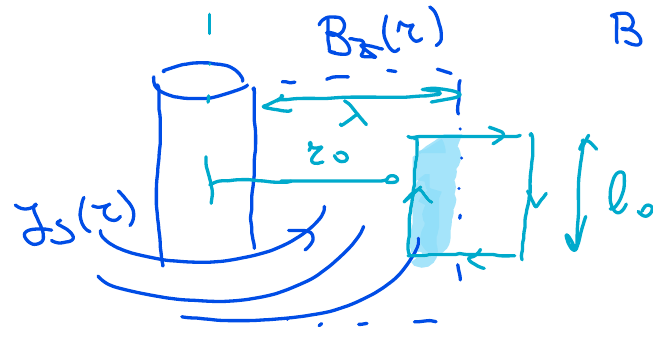
\includegraphics[width=0.5\textwidth]{immagini/cammino_di_integrazione_B_Pippard.png}
\end{figure}
\hspace{-0.6cm}Assumiamo che appena fuori (cioè per $r>\lambda$) il campo magnetico sia praticamente nullo. Se assumiamo che nella regione esterna $\vb{B}$ sia già decaduto, l'integrale di linea di $\vb{B}$ si riduce all'integrale lungo il lato interno parallelo all'asse $z$ che avrà una certa lunghezza che chiamiamo $l_0$,\mn{Il contributo negli altri due lati è zero perché essendo perpendicolari a $\vb{B}$ il prodotto scalare è nullo, il contributo lungo l'altro lato parallelo che si trova nella regione esterna è molto più piccolo e quindi trascurabile.} come mostrato nella figura precedente. In definitiva abbiamo
\begin{equation*}
   \oint \vb{B} \vdot \dd{\vb{l}}
   \approx B_z(r_0) l_0
\end{equation*}
Per la legge di Amper, esso sarà uguale al flusso della densità di corrente che passa attraverso la regione evidenziata in figura, dunque si ha
\begin{equation*}
   B_z(r) l_0
   =\mu_0 l_0 \int_{r_0}^{\lambda} J_s(r) \dd{r}
\end{equation*}
Per l'approssimazione fatta nell'\eqrefcustom{eq:campo_magnetico_vortex_interno}, sappiamo che che $B_z(r_0)$ si può esprimere come
\begin{equation*}
   B_z(r_0)
   =\frac{\Phi_0}{2\pi \lambda^2} \ln\qty(\frac{\lambda}{r_0})
\end{equation*}
quindi $\vb{J}_s$, che integrata ci deve dare il logaritmo, deve essere una funzione che va come $\frac{1}{r}$. Possiamo supporre dunque che
\begin{equation*}
   J_s(r)
   =\frac{a}{r}
\end{equation*}
Svolgendo allora i calcoli, quello che troviamo da legge di Ampere è che
\begin{equation*}
   \frac{l_0 \Phi_0}{2\pi \lambda^2} \ln\qty(\frac{\lambda}{r_0})
   =\mu_0 l_0 a \ln\qty(\frac{\lambda}{r_0})
\end{equation*}
da cui ricaviamo che
\begin{equation*}
   a
   =\frac{\Phi_0}{2\pi \mu_0 \lambda^2}
\end{equation*}
e pertanto la densità di corrente nella regione per $\xi_0 < r < \lambda$ è
\begin{equation*}
   \vb{J}_s(r)
   =\frac{\Phi_0}{2\pi \mu_0 \lambda^2} \frac{1}{r} \vu{u}_{\varphi}
   %\label{eq:densita_corrente_vortex_interno}
\end{equation*}
Cerchiamo allora di capire com'è fatto questo vortice di London:
\begin{itemize}[leftmargin=0.5cm]
   \item per $r<\xi_0$ abbiamo una regione normale in cui c'è il campo magnetico che è praticamente uniforme e pari a $\frac{\Phi_0}{\pi \xi_0^2}$;
   \item per $\xi_0 < r < \lambda$ abbiamo un campo magnetico che va come $\ln(\lambda/r)$ e una densità di corrente che va come $\frac{1}{r}$ ed è diretta a formare un vortice;
   \item per $r>\lambda$ abbiamo un decadimento esponenziale del campo magnetico.
\end{itemize}
In conclusione, la teoria di London può essere applicata anche ad un superconduttore del secondo tipo per descrivere cosa succede in corrispondenza dei vortici, che sono quelli che descrivono la penetrazione del campo magnetico nei superconductori del secondo tipo. Questa teoria di London non dice perché abbiamo questa struttura (noi siamo partiti dal supporre che ci sia questa struttura e abbiamo legato tra loro il campo magnetico e densità di corrente). La giustificazione al fatto che si ha la penetrazione del campo magnetico con queste strutture quando siamo nella condizione di superconduttore del secondo tipo ce la dirà la teoria di Ginzburg--Landau.
\subsection{Risposta AC dei superconduttori. Modello a due fluidi di Gorter e Casimir}
Fino ad ora abbiamo sostanzialmente considerato la risposta statica del campo magnetico, sebbene siamo partiti dalla conducibilità dipendente dalla frequenza in un metallo normale, abbiamo poi trattato questo metallo normale come un materiale in cui il tempo medio tra gli urti va a infinito, abbiamo approssimato la conducibilità sotto tali condizioni e poi abbiamo guardato al limite di risposta a frequenza nulla, cioè alla risposta statica.\\
In realtà nella maggior parte dei casi si ha a che fare con campi magnetici variabili nel tempo e il punto è che tutte le volte che noi abbiamo un campo magnetico variabile nel tempo la risposta del materiale non è la semplice risposta superconduttiva che abbiamo visto adesso, ma c'è anche una piccola componente di corrente dissipativà. Questo comportamento, che viene fuori anch'esso rigorosamente dalla teoria BCS, può essere descritto da una teoria basata sul nuovo modello dei due fluidi che descrive il materiale che diviene superconduttivo come un materiale che ha sia una componente normale che una componente superconduttiva, le quali hanno entrambe una risposta espressa da una conducibilità che è quella data dal modello di Drude per il materiale normale ma anche per il materiale superconduttivo, dove per il materiale superconduttivo si prende la risposta che otteniamo dall'espressione per il materiale normale mandando ad infinito il tempo medio tra gli urti. Quello che allora faremo adesso è, a partire da questo modello di due fluidi a frequenza finita, cercare di capire in quali regimi abbiamo una risposta dissipativa e in quali no, nel caso in cui abbiamo un campo variabile nel tempo.\\
Supponiamo di guardare la risposta alle differenti frequenze, dunque la risposta AC. Per inciso la teoria BCS prevede questo comportamento e lo attribuisce a effetti nati dall'eccitazione termica.\\
L'idea del modello dei due fluidi consiste nel considerare il materiale superconduttore come formato da questi due fluidi, i quali sono uno nello stato normale, quindi con la conducibilità tipica per un metallo normale, ovvero
\begin{equation*}
   \sigma_n(\omega)
   =\frac{n_n e^2 \tau_n}{m} \frac{1}{1 + i\omega \tau_n}
   =\frac{\sigma_n}{1 + i\omega \tau_n}
\end{equation*}
e uno nello stato superconduttivo che ha conducibilità avente una parte reale e una parte immaginaria che abbiamo ricavato da questo modello per $\tau \to \infty$ date da
\begin{equation*}
   \sigma_s(\omega)
   \sigma_{s,\text{Re}} - i \sigma_{s,\text{Im}}
   \approx \frac{\pi n_s e^2}{2 m} \delta(\omega) - i \frac{n_s e^2}{m \omega}
\end{equation*}
Considerare frequenze finite ma sufficientemente basse, con cui si intende considerare il regime $\omega \tau_n \ll 1$, $\tau_n$ è il tempo medio tra gli urti di un metallo normale che è dell'ordine di $10^{-12} \; \rm s$. Essendo $\omega \tau_n$ molto piccolo, possiamo appossimare la risposta del materiale normale con la sua parte reale, quindi la conducibilità totale sarà
\begin{equation*}
   \sigma(\omega)
   =\bigl[ \sigma_{s,\,\text{Re}} + \sigma_n(\omega) \bigr] - i \sigma_{s,\,\text{Im}}
   \approx \qty[ \frac{\pi n_s e^2}{2 m} \delta(\omega) + \frac{n_n e^2 \tau_n}{m}] - i \frac{n_s e^2}{m \omega}
\end{equation*}
dunque l'unico termine immaginario in questa approssimazione è quello proveniente dalla risposta del superconduttore. Sebbene questa sia una descrizione molto semplificata, essa ci dice che se guardiamo la parte reale della risposta, cioè quella che ci dà la dissipazione, essa ci dice che se siamo a frequenza nulla, dunque nel caso di risposta DC, quello che rimane è la parte reale del comportamento superconduttivo, quindi abbiamo una supercorrente e non c'è dissipazione; se invece siamo a frequenza finite diverse da zero, seppur piccole, abbiamo una risposta che ci proviene anche dalla parte normale, il quale corrisponde a un comportamento dissipativo.\\
Vediamo come capire quale dei due contributi prevale a seconda della frequenza. Supponendo che per ciascuna componente valga $\vb{J}(\omega)=\sigma(\omega)\vb{E}(\omega)$, calcoliamo il rapporto tra la componente superconduttiva e quella normale della densità di corrente. Suponendo che il campo sia lo stesso e di trovarci a frequenza finita ossia per $\omega \neq 0$,\mn{Ciò significa che resta soltanto la parte immaginaria di $\sigma_s(\omega)$, e ciò è dovuto alla presenza della $\delta(\omega)$ nella parte reale.} si trova che
\begin{equation}
   \frac{J_s(\omega)}{J_n(\omega)}
   =\frac{\sigma_{s,\text{Im}}}{\sigma_{n,\text{Re}}}
   =\frac{n_s}{n_n} \frac{1}{\omega \tau_n}
   \label{eq:rapporto_correnti_superconduttiva_normale}
\end{equation}
Tale espressione ci permette di capire che queste due correnti sono paragonabili quando
\begin{equation*}
   \omega_c
   \approx \frac{n_s}{n_n} \frac{1}{\tau_n}
\end{equation*}
Conosciamo il valore di $\tau_n$, e se supponiamo che $n_s$ e $n_n$ siano più o meno dello stesso ordine, possiamo stimare che la frequenza di crossover $\omega_c$ è dell'ordine di $10^{12} \; \rm Hz$, quindi ricade nella regione delle microonde.\\
In definitiva, l'\eqrefcustom{eq:rapporto_correnti_superconduttiva_normale} ci dice che
\begin{itemize}[leftmargin=0.5cm]
   \item se abbiamo dei campi a frequenze più basse di $\omega_c$, la componente superconduttiva della corrente prevale su quella normale, cioè $J_s(\omega)>J_n(\omega)$. Avremo comunque una componente normale, ma la risposta del materiale sarà prevalentemente superconduttiva;
   \item se abbiamo dei campi a frequenze più alte di $\omega_c$, la componente normale della corrente prevale su quella superconduttiva, cioè $J_n(\omega)>J_s(\omega)$. In questo caso avremo una risposta prevalentemente normale, con una piccola componente superconduttiva.
\end{itemize}
Questo modello a due fluidi ci permette allora di avere un'idea del range di frequenze, dunque del range di rapidità di variazione dei campi, nei quali possiamo aspettarci un comportamento superconduttivo o un comportamento normale, fermo restando che dobbiamo sempre prevedere una piccola componente dissipativa secondo.\\
In realtà, assumere che le due densità siano pressocché uguali non è sempre corretto, perché dal confronto con i risultati sperimentali sulla lunghezza di penetrazione e la sua dipendenza dalla temperatura possiamo dedurre una dipendenza dalla temperatura della densità degli elettroni superconduttivi che è proporzionare a $(T/T_c)^4$, da cui si ricava che la componente normale ha una dipendenza del tipo
\begin{equation*}
   n_n(T)
   \propto 1 - \qty(\frac{T}{T_c})^4
\end{equation*}
tale dipendenza nasce dal fatto che la somma delle due densità deve essere indipendente dalla temperatura e sia la densità complessiva degli elettroni.\\
Questi andamenti in realtà sono approssimati. La teoria BCS ci dà un andamento di tipo esponenziale che è
\begin{equation*}
   n_n(T)
   \propto e^{-\frac{\Delta}{k_B T}}
\end{equation*}
dove $\Delta$ è la gap superconduttiva. Ciò ovviamente non può venir fuori da una teoria fenomenologica perché non c'è una ragione ovvia per la quale ipotizzare che ci sia una gap energetica che separa il comportamento di questi materiali da una parte e dall'altra.
\section{Teoria di Ginzburg--Landau}
Finora abbiamo descritto la transizione superconduttiva come una transizione di fase e abbiamo visto che, a seconda della presenza o meno di un campo magnetico, essa può essere del primo o del secondo ordine. Tuttavia, non abbiamo ancora discusso in che modo una descrizione dei materiali superconduttori in termini di un potenziale termodinamico, ossia una teoria basata sulla teoria delle transizioni di fase, possa prevedere l'esistenza di queste fasi e determinarne le proprietà.\\
La teoria di Ginzburg--Landau affronta proprio questo problema. Essa si basa sull'approccio fenomenologico di Landau alle transizioni di fase e lo applica alla superconduttività, con l'obiettivo di descrivere il comportamento di un materiale metallico in presenza di un campo magnetico e di comprendere come avvenga la transizione tra la fase normale e quella superconduttiva.\\
Un aspetto essenziale della teoria è che essa tiene conto della possibilità che il campo magnetico all'interno del materiale non sia uniforme. Questo è precisamente ciò che accade nella fase superconduttiva: a causa dell'effetto Meissner, il campo magnetico viene espulso dall'interno del materiale e rimane confinato solo in determinate regioni. La teoria di Ginzburg--Landau fornisce quindi un quadro termodinamico in grado di descrivere sia la transizione di fase sia la distribuzione spaziale del campo magnetico nel materiale.
\subsection{Transizioni di fase}
L'idea è quella di considerare la fase normale e quella superconduttiva come due diverse fasi del materiale, separate da una transizione di fase. Esse possono quindi essere descritte mediante un potenziale termodinamico caratterizzato dal fatto che, nel punto di transizione, assume lo stesso valore nelle due fasi.\\
Per sviluppare questa descrizione ci basiamo sulla teoria delle transizioni di fase del secondo ordine della meccanica statistica, il cui esempio più noto è la transizione ferromagnetica. In un materiale ferromagnetico, se la temperatura è maggiore di una certa temperatura critica $T_c$, il sistema non presenta alcuna magnetizzazione macroscopica. Tuttavia, se la temperatura scende al di sotto di $T_c$, il sistema sviluppa spontaneamente una magnetizzazione in una determinata direzione.\\
Questo fenomeno avviene anche in assenza di un campo magnetico esterno ed è associato a una rottura spontanea di simmetria. Infatti, a temperature elevate il sistema non possiede una direzione privilegiata nello spazio, mentre la comparsa di una magnetizzazione spontanea introduce una direzione preferenziale. Il sistema passa quindi da uno stato più simmetrico a uno stato meno simmetrico.\\
Un comportamento analogo si ritrova nella transizione superconduttiva.\\
Per comprendere come emerga questa rottura spontanea di simmetria, consideriamo l'approccio fenomenologico proposto da Landau. In tale approccio si introduce un parametro d'ordine che caratterizza lo stato macroscopico del sistema. Nel caso del ferromagnetismo questo parametro è la magnetizzazione.\\
L'idea è quindi quella di introdurre una densità di energia libera che dipende dal parametro d'ordine. A temperature maggiori della temperatura critica questa energia libera presenta un unico minimo, che corrisponde alla configurazione con parametro d'ordine nullo. Nel caso del ferromagnetismo ciò significa che la magnetizzazione è nulla.\\
Quando invece la temperatura scende al di sotto della temperatura critica, la forma della funzione cambia: la dipendenza dell'energia libera dal parametro d'ordine passa da una struttura con un unico minimo a una struttura con due minimi degeneri corrispondenti a valori non nulli del parametro d'ordine.
\begin{figure}[H]
   \centering
   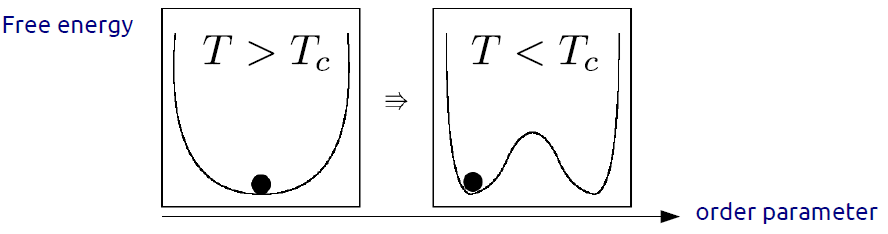
\includegraphics[width=0.9\textwidth]{immagini/andamento_energia_libera_parametro_dordine.png}
\end{figure}
\hspace{-0.6cm}Nel caso della magnetizzazione ciò significa che, al di sotto della temperatura critica, il sistema sceglie spontaneamente una delle configurazioni di energia minima, corrispondente a una magnetizzazione diversa da zero orientata in una certa direzione.\\
Il parametro $\psi$ che descrive questo cambiamento dello stato del sistema è detto parametro d'ordine. Nel caso del ferromagnetismo esso può essere identificato con la magnetizzazione, che è nulla per $T>T_c$ e diversa da zero per $T<T_c$.\\
Parliamo ora in termini più generali della teoria di Landau delle transizioni di fase. Introduciamo un parametro d'ordine $\psi$.\mn{Nella teoria di Ginzburg--Landau esso è un oggetto complesso; per il momento possiamo tuttavia considerarlo reale. Nel caso del ferromagnetismo esso corrisponde al modulo della magnetizzazione, $|\vb{M}|$.}\\
La teoria di Landau consiste nello scrivere la densità di energia libera come funzione del parametro d'ordine. Nel caso della superconduttività si può scrivere
\begin{equation}
   f_s = f_n + a |\psi|^2 + \frac{b}{2} |\psi|^4
   \label{eq:energia_libera_Ginzburg_Landau}
\end{equation}
dove $f_n$ è la densità di energia libera della fase normale e gli altri termini rappresentano il contributo associato allo stato superconduttivo.\\
L'idea alla base della teoria delle transizioni di fase del secondo ordine è quella di sviluppare l'energia libera della nuova fase in serie di Taylor rispetto al parametro d'ordine intorno allo stato normale. Si includono i termini quadratici e quartici perché questa è la struttura più semplice che permetta di descrivere la comparsa di nuovi minimi dell'energia libera.\\
In particolare, il coefficiente $b$ rimane positivo, mentre il coefficiente $a$ dipende dalla temperatura secondo la legge
\begin{equation*}
   a(T) = a' \frac{T-T_c}{T_c},
   \qq{con} a' > 0
\end{equation*}
In questo modo $a$ risulta positivo per $T>T_c$ e negativo per $T<T_c$.
\begin{figure}[H]
   \centering
   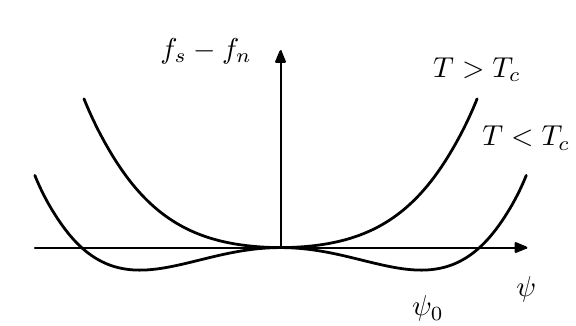
\includegraphics[width=0.6\textwidth]{immagini/differenze_energie_libere.png}
\end{figure}
\hspace{-0.6cm}Se $T>T_c$, la differenza tra le densità di energia libera delle due fasi presenta un unico minimo in corrispondenza di $\psi=0$, che corrisponde alla fase normale.\\
Se invece $T<T_c$, il coefficiente $a$ diventa negativo e la funzione assume la tipica forma a doppia buca. I minimi si trovano per valori non nulli del parametro d'ordine. Per determinarli calcoliamo i valori in corrispondenza dei quali la differenza tra le energie libere delle due fasi è minima, ossia calcoliamo i punti in cui la derivata rispetto a $|\psi|$ si annulla:
\begin{equation*}
   \dv{(f_s - f_n)}{|\psi|}
   =2a |\psi| + 2b |\psi|^3 =0
\end{equation*}
Da questa relazione otteniamo
\begin{equation*}
   |\psi_{\rm min}|^2 = -\frac{a}{b} > 0
\end{equation*}
che è positivo perché $a<0$ per $T<T_c$.\\
Sostituendo l'espressione di $a(T)$ si trova
\begin{equation*}
   \psi_{\rm min}
   =\sqrt{\frac{a'(T_c-T)}{b T_c}}
\end{equation*}
Infine, sostituendo questo valore nell'energia libera si ottiene
\begin{equation*}
   f_s
   = f_n - \frac{{a'}^2}{2b} \qty(\frac{T_c-T}{T_c})^2
\end{equation*}
Da questa espressione si vede che per $T<T_c$ la fase superconduttiva ha energia libera più bassa rispetto alla fase normale ed è quindi termodinamicamente stabile, mentre per $T>T_c$ è stabile la fase normale.
\subsection{Teoria di Ginzburg--Landau per la superconduttività}
L'idea è quella di descrivere la transizione dalla fase normale alla fase superconduttiva di un metallo come una transizione di fase. Per farlo consideriamo una descrizione termodinamica del materiale. In altre parole, per descrivere la transizione di fase dobbiamo introdurre un'energia libera che descriva il sistema che stiamo studiando, identificando quali sono i parametri rilevanti che guidano la transizione. In questo caso tali parametri sono in particolare la temperatura e il campo magnetico. Sappiamo infatti che la transizione dalla fase normale alla fase superconduttiva avviene diminuendo la temperatura; essa è quindi uno dei parametri che possiamo variare per indurre la transizione. L'altro parametro è il campo magnetico, poiché sappiamo che la transizione può avvenire solo se il campo magnetico è inferiore a un certo campo critico che dipende dalla temperatura.\\
L'idea è quindi quella di considerare queste due fasi come diverse fasi termodinamiche del metallo, separate da una transizione di fase. L'evidenza della transizione di fase si manifesta nelle grandezze termodinamiche, in particolare nel calore specifico del superconduttore, come vedremo più avanti.\\
Applichiamo ora la teoria di Ginzburg--Landau alla transizione dalla fase normale alla fase superconduttiva e dobbiamo identificare il parametro d'ordine appropriato $\psi$. Questa teoria fu sviluppata nel 1950 ed è estremamente ingegnosa, nel senso che a quel tempo non si conosceva ancora il meccanismo microscopico responsabile della superconduttività. Tuttavia si intuiva già che il fenomeno dovesse avere un'origine quantistica. L'idea era quindi che la superconduttività fosse un fenomeno di natura quantomeccanica, pur non conoscendo ancora il motivo preciso per cui si verificasse, e che mostrasse una transizione di fase analoga a quelle note nei sistemi classici.\\
Si cercò quindi di identificare un parametro d'ordine che descrivesse le configurazioni macroscopiche stabili del sistema. Tenendo presente la natura quantistica del fenomeno, si assunse che il parametro d'ordine fosse una quantità complessa $\psi$, con l'idea che potesse svolgere il ruolo di una funzione d'onda che descrive la fase superconduttiva. In altre parole, si utilizzò come parametro d'ordine una quantità che, in qualche modo, potesse essere interpretata come una funzione d'onda macroscopica del sistema.\mn{A questo livello, per funzione d'onda si intende semplicemente un parametro d'ordine complesso.}\\
Questa intuizione era anche influenzata dagli sviluppi teorici relativi alla superfluidità dell'elio $^4\mathrm{He}$. Infatti la teoria della superfluidità era stata sviluppata prima di quella della superconduttività, e in quel contesto era stata introdotta una funzione d'onda macroscopica per descrivere il fluido superfluido. L'idea di una funzione d'onda macroscopica per il superconduttore fu quindi ispirata anche da questi risultati.\\
Circa dieci anni più tardi fu possibile dimostrare che il parametro d'ordine della teoria di Ginzburg--Landau è effettivamente legato alla densità locale dei portatori di carica nel superconduttore. In particolare si trovò che $|\psi|^2$ è proporzionale alla densità degli elettroni superconduttivi.\\
Cominciamo quindi scrivendo la densità di energia libera $f$ in funzione del parametro d'ordine complesso. L'energia libera che utilizziamo è l'energia libera di Gibbs, poiché abbiamo visto che essa è il potenziale termodinamico appropriato per descrivere una transizione guidata da variazioni di temperatura e di campo magnetico applicato $H$.\\
Vogliamo quindi scrivere l'energia libera di Gibbs della fase superconduttiva come funzione dell'energia libera della fase normale più alcuni contributi che dipendono dal parametro d'ordine $\psi$. In altre parole, ci aspettiamo che l'energia libera sia una funzione del parametro d'ordine.\\
Per determinare la forma di questa dipendenza consideriamo le seguenti ipotesi:
\begin{itemize}[leftmargin=0.5cm]
   \item $f_s$ deve coincidere con l'energia libera della fase normale $f_n$ quando il parametro d'ordine tende a zero, cioè quando $\psi \to 0$ (per semplicità, per il momento supponiamo $\psi$ reale);
   \item Sappiamo che la transizione avviene modificando la temperatura, quindi possiamo supporre che $f_s$ sia dato da $f_n$ più un contributo che dipende almeno dalla temperatura (per il momento trascuriamo il campo magnetico);
   \item La differenza $f_s - f_n$, considerata come funzione di $\psi$, deve essere una funzione simmetrica che per $T>T_c$ possiede un unico minimo stabile in $\psi=0$ (quindi deve avere una forma parabolica), mentre per $T<T_c$ deve presentare una rottura di simmetria, cioè una funzione simmetrica con minimi per valori di $\psi$ diversi da zero. Inoltre la forma della funzione deve cambiare in modo continuo al variare della temperatura.
\end{itemize}
La funzione più semplice che possiede queste proprietà può essere ottenuta sviluppando la densità di energia libera in serie di Taylor attorno allo stato normale. Per ottenere un comportamento parabolico è necessario un termine quadratico, quindi il primo contributo può essere scritto nella forma $a\psi^2$, dove $a$ è una funzione della temperatura tale che il potenziale abbia la forma desiderata. In particolare $a$ deve essere proporzionale a $T-T_c$, in modo da risultare positivo per $T>T_c$.\\
Quando la temperatura scende al di sotto di $T_c$, la differenza $f_s - f_n$ deve invece assumere la forma a doppia buca mostrata in precedenza. Per ottenere questo comportamento è necessario aggiungere un termine quartico $b\psi^4$.\\
Il coefficiente $b$ deve essere positivo affinché il sistema abbia una fase stabile per $\psi=0$ quando $T>T_c$. Quando invece $T<T_c$, il sistema avrà una fase stabile con un valore non nullo di $\psi$.\\
Vediamo più precisamente come emerge questa struttura. Il minimo di $f_s - f_n$ si trova imponendo
\begin{equation*}
   \dv{(f_s-f_n)}{\psi}
   =2a\psi + 2b\psi^3
   =2\psi(a+b\psi^2)
   =0
\end{equation*}
da cui segue che o $\psi=0$ oppure
\begin{equation*}
   \psi^2=-\frac{a}{b}
\end{equation*}
Poiché $\psi^2$ deve essere positivo, questa soluzione è possibile solo quando $a<0$. Scrivendo
\begin{equation*}
   a(T)=a'\frac{T-T_c}{T_c}
\end{equation*}
si ottiene
\begin{equation*}
   \psi^2
   =-\frac{a'}{b}\frac{T-T_c}{T_c}
\end{equation*}
che è positivo solo per $T<T_c$.\\
Questo significa che per $T>T_c$ il minimo si trova in $\psi=0$, cioè le energie libere delle due fasi coincidono e la fase stabile è quella normale. Per $T<T_c$, invece, la soluzione stabile corrisponde a un valore non nullo del parametro d'ordine.\\
Sostituendo questo valore nell'energia libera si ottiene
\begin{equation}
   f_s
   =f_n - \frac{{a'}^2}{2b}\left(\frac{T_c-T}{T_c}\right)^2
   \label{eq:free_energy_ginzburg_landau}
\end{equation}
La relazione \eqrefcustom{eq:free_energy_ginzburg_landau} mostra che la densità di energia libera della fase superconduttiva è minore di quella della fase normale quando $T<T_c$, e quindi la fase stabile è quella superconduttiva.\\
In questo modo, applicando la teoria di Landau delle transizioni di fase del secondo ordine, riusciamo a descrivere in modo fenomenologico il comportamento dei superconduttori che subiscono una transizione di fase a campo magnetico nullo quando $T<T_c$.\\
C'è però un aspetto importante da ricordare. Finora abbiamo introdotto il parametro d'ordine complesso come un'intuizione basata sulla natura quantistica del fenomeno. Il fatto che il parametro sia complesso implica che possiamo scriverlo nella forma\\
\begin{equation*}
   \psi = |\psi| e^{i\vartheta}
\end{equation*}
Osserviamo però che l'energia libera dipende solo da $|\psi|^2$, quindi non dipende dalla fase $\vartheta$, ma soltanto dall'ampiezza.\\
Questo significa che, quando avviene la transizione alla fase superconduttiva, il parametro d'ordine assume un valore
\begin{equation*}
   \psi_s = |\psi_s| e^{i\vartheta_s}
\end{equation*}
dove $|\psi_s|$ è determinato dalla condizione di minimo dell'energia libera, mentre la fase $\vartheta_s$ può assumere un valore arbitrario.\\
Anche se la fase non compare esplicitamente nell'energia libera, essa esiste nel parametro d'ordine che descrive la fase superconduttiva. Di conseguenza, quando avviene la transizione il sistema deve scegliere spontaneamente un valore della fase.\\
Questo è, in una certa misura, analogo a ciò che accade nella transizione ferromagnetica: in quel caso il sistema sceglie spontaneamente una direzione della magnetizzazione. Nel caso della transizione superconduttiva, invece, il sistema sceglie spontaneamente una fase. Vedremo più avanti che questa fase ha un significato fisico molto importante, nonostante in meccanica quantistica siamo spesso abituati a considerare la fase della funzione d'onda come non rilevante.
\subsection{Proprietà termodinamiche}
La prima cosa che dobbiamo verificare è se la dipendenza dell'energia libera dalla temperatura, data dall'\eqrefcustom{eq:free_energy_ginzburg_landau}, sia in grado di descrivere le proprietà termodinamiche dei superconduttori, e in particolare il calore specifico.
\begin{figure}[H]
   \centering
   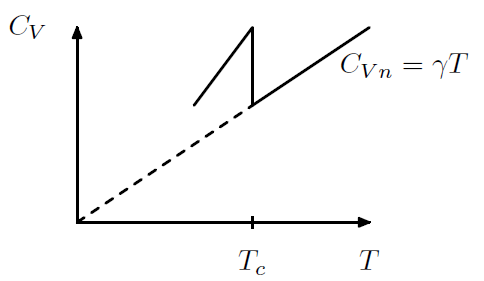
\includegraphics[width=0.6\textwidth]{immagini/calore_specifico_ginzburg_landau.png}
   \caption*{Calore specifico di un superconduttore in prossimità di $T_c$ nel modello di Ginzburg--Landau. Al di sopra di $T_c$ il calore specifico è quello previsto dalla teoria di Sommerfeld dei metalli, $C_{V,n}=\gamma T$. In corrispondenza di $T_c$ si osserva una discontinuità e un cambiamento della pendenza.}
\end{figure}
\hspace{-0.6cm}Abbiamo visto che una delle evidenze della transizione alla fase superconduttiva si manifesta anche nelle proprietà termodinamiche. In particolare, osservando l'andamento del calore specifico in funzione della temperatura, si nota che per $T>T_c$ il sistema presenta la tipica dipendenza lineare dalla temperatura, che corrisponde al comportamento normale dei metalli. Per temperature inferiori a $T_c$ (e in particolare in corrispondenza di $T=T_c$) si osserva invece una discontinuità nel calore specifico.\\
Questa discontinuità è un'indicazione della presenza di una transizione di fase e costituisce quindi una evidenza termodinamica della transizione superconduttiva.\\
Avendo a disposizione un'espressione per l'energia libera, possiamo derivarne il calore specifico e verificare se la dipendenza dalla temperatura che abbiamo ottenuto è in grado di descrivere questo salto nel calore specifico.\\
Abbiamo visto, attraverso l'\eqrefcustom{eq:relazione_termodinamica_campo_critico}, che la differenza tra le energie libere delle due fasi è anche legata alla densità di energia magnetica. In particolare, quando il campo magnetico applicato è uguale al campo critico alla temperatura considerata, vale la relazione
\begin{equation*}
   f_s(T,H_c)
   - f_n(T,H_c)
   =-\frac{H_c^2(T)}{8\pi}
\end{equation*}
Consideriamo ora il calore specifico. Per calcolarlo dobbiamo studiare la variazione dell'energia libera, cioè $\dd f$. Poiché l'energia libera dipende dalla temperatura e dal campo magnetico, $f=f(T,B)$, la sua variazione è data da
\begin{equation*}
   \dd{f}
   = -s\,\dd{T} + \frac{H}{4\pi} \dd{B}
\end{equation*}
Da questa relazione si vede immediatamente che il calore specifico è dato da
\begin{equation*}
   C
   =T\qty(\pdv{s}{T})_B
   =-T\qty(\pdv[2]{f}{T})_B
\end{equation*}
Ciò significa che, per determinare il calore specifico del superconduttore utilizzando l'\eqrefcustom{eq:free_energy_ginzburg_landau}, è sufficiente calcolare la derivata seconda dell'energia libera rispetto alla temperatura e moltiplicarla per $T$. Si ottiene così
\begin{equation*}
   C_s - C_n
   =- T \pdv[2]{T}
   \qty[ -\frac{{a'}^2}{2b} \qty(\frac{T_c-T}{T_c})^2 ]
   =- \frac{{a'}^2}{b}\frac{T}{T_c^2}
\end{equation*}
La differenza tra il calore specifico nella fase superconduttiva e quello nella fase normale alla temperatura critica risulta quindi
\begin{equation*}
   \bigl[ C_s - C_n \bigr]_{T=T_c}
   =\frac{{a'}^2}{b}\frac{1}{T_c}
\end{equation*}
il che mostra esplicitamente la presenza di un salto nel calore specifico in corrispondenza della temperatura critica.
\subsection{Sistemi non omogenei}
Finora abbiamo considerato $\psi$ come un parametro d'ordine uniforme. In realtà, la teoria di Ginzburg--Landau è in grado di descrivere anche variazioni spaziali della fase superconduttiva. Essa può quindi descrivere situazioni in cui il sistema presenta regioni che sono superconduttive e regioni che non lo sono.\\
Abbiamo già incontrato un esempio semplice di questa situazione quando abbiamo considerato il caso idealizzato di un superconduttore che occupa un semispazio, con il vuoto dall'altra parte. In quel caso abbiamo visto che il campo magnetico penetra nel materiale per una certa distanza dalla superficie. In prossimità della superficie è presente una corrente schermante e può esistere una regione del materiale che non è completamente nello stato superconduttivo, mentre più all'interno il materiale è pienamente superconduttivo.\\
Anche in situazioni molto semplici è quindi necessario poter descrivere un sistema che presenta regioni normali e regioni superconduttive.\\
Per farlo, in questa teoria dobbiamo introdurre un parametro d'ordine complesso che varia nello spazio. Questo è uno dei punti di forza della teoria di Ginzburg--Landau: essa è in grado di descrivere correttamente situazioni in cui il parametro d'ordine cambia nello spazio, purché ci si trovi a temperature vicine alla temperatura critica.\\
L'idea è quindi che il parametro d'ordine diventa una funzione della posizione. Pertanto, esso avrà sia un'ampiezza sia una fase che dipendono dalla posizione:
\begin{equation*}
   \psi
   \equiv \psi(\vb{r})
   = |\psi(\vb{r})| e^{i\vartheta(\vb{r})}
\end{equation*}
La domanda è quindi come questa dipendenza dalla posizione entri nell'espressione dell'energia libera. L'intuizione è la seguente: se immaginiamo che questa funzione descriva l'intero superconduttore, cioè lo stato macroscopico formato da un grandissimo numero di elettroni, allora possiamo identificare il modulo quadro di questa quantità, $|\psi(\vb{r})|^2$, con la densità locale di elettroni superconduttivi.\\
Questa idea è ispirata dall'analogia con la meccanica quantistica. Infatti, se $\psi$ è la funzione d'onda di una singola particella, allora $|\psi|^2$ rappresenta la densità di probabilità di trovare la particella nello spazio. Se invece immaginiamo di avere una funzione d'onda macroscopica che descrive il condensato superconduttivo, è naturale interpretare il modulo quadro di tale funzione come la densità locale degli elettroni superconduttivi.\\
Se adottiamo questa interpretazione e pensiamo all'energia libera del superconduttore come alla somma di tutti i contributi energetici rilevanti, è naturale includere nell'energia libera un termine che ricordi l'energia cinetica di una particella.\mn{\cite{Annett} Ginzburg e Landau postularono che l'energia libera avesse la forma dell'\eqrefcustom{eq:energia_libera_Ginzburg_Landau}, a cui si aggiunge un nuovo termine dipendente dal gradiente di $\psi(\vb{r})$.}\\
Seguendo questa prospettiva, dobbiamo quindi introdurre un termine che dipenda dal gradiente di $\psi$. In meccanica quantistica, infatti, l'energia di una particella libera è $\frac{\vb{p}^2}{2m}$ e l'operatore impulso è legato al gradiente della funzione d'onda.\\
L'idea è quindi che, per descrivere situazioni in cui il parametro d'ordine varia nello spazio, si debba includere nell'espressione della densità di energia libera del superconduttore un termine analogo a un contributo di energia cinetica. Si ottiene così
\begin{equation}
   f_s(\vb{r})
   = f_n
   + \frac{\hbar^2}{2m^*} |\grad{\psi}|^2
   + a(T) |\psi|^2
   + \frac{b(T)}{2} |\psi|^4
   \label{eq:free_energy_ginzburg_landau_inhomogeneous}
\end{equation}
Notiamo che abbiamo introdotto una massa $m^*$, che rappresenta la massa efficace dei portatori di carica nel superconduttore. All'epoca della formulazione della teoria non era possibile determinarne il valore. Vedremo in seguito che questa massa efficace corrisponde in realtà alla massa di due elettroni.\\
Questo termine può essere compreso anche da un punto di vista più matematico, considerando nuovamente l'energia libera come una sorta di espansione in serie di Taylor. Se infatti il parametro d'ordine dipende da un'altra variabile, in particolare dalla posizione, è naturale che compaiano contributi aggiuntivi legati alle derivate spaziali di $\psi$, cioè al gradiente di $\psi$.
\subsection{Derivazione delle equazioni di Ginzburg--Landau}
Il nostro obiettivo è ora determinare la funzione $\psi(\vb{r})$ che minimizza l'energia libera. La situazione è più complessa rispetto al caso precedente, in cui avevamo semplicemente un potenziale a doppia buca, poiché ora il parametro d'ordine può variare nello spazio.\\
Possiamo scrivere l'energia libera come integrale nello spazio della densità di energia libera. In questo modo l'espressione \eqrefcustom{eq:free_energy_ginzburg_landau_inhomogeneous} diventa
\begin{equation}
   F_s(T)
   = F_n(T) + \int \dd[3]{\vb{r}} \qty(
   \frac{\hbar^2}{2m^*} |\grad{\psi}|^2
   + a(T) |\psi(\vb{r})|^2
   + \frac{b(T)}{2} |\psi(\vb{r})|^4
   )
   \label{eq:differenza_energie_libere_integrata}
\end{equation}
Per trovare la funzione $\psi(\vb{r})$ che minimizza l'energia libera utilizziamo un approccio variazionale. Consideriamo quindi una variazione infinitesima del parametro d'ordine:
\begin{equation}
   \psi(\vb{r})
   \to \psi(\vb{r}) + \delta \psi(\vb{r})
   \label{eq:variazione_parametro_dordine}
\end{equation}
e calcoliamo la variazione dell'energia libera al primo ordine in $\delta\psi$. La condizione di minimo richiede che tale variazione sia nulla.\\
Sostituendo $\psi$ e $\psi^*$ nella forma dell'\eqrefcustom{eq:variazione_parametro_dordine} all'interno dell'\eqrefcustom{eq:differenza_energie_libere_integrata} e mantenendo solo i termini al primo ordine in $\delta\psi$ e $\delta\psi^*$, si ottiene
\begin{equation*}
   \begin{split}
      \delta F_s
      &= \int \dd[3]{\vb{r}} \qty[
      \frac{\hbar^2}{2m^*} (\grad{\delta \psi^*}) \cdot (\grad{\psi})
      + \delta \psi^* \qty( a\psi + b \psi |\psi|^2 )
      ]
      \\
      &\quad + \int \dd[3]{\vb{r}} \qty[
      \frac{\hbar^2}{2m^*} (\grad{\psi^*}) \cdot (\grad{\delta \psi})
      + \delta \psi \qty( a\psi^* + b \psi^* |\psi|^2 )
      ]
   \end{split}
\end{equation*}
Il passo successivo consiste nel semplificare queste espressioni mediante integrazione per parti. Trascurando i termini di superficie (assumendo condizioni al contorno appropriate), si ottiene
\begin{equation}
\begin{split}
   \delta F_s
   &= \int \dd[3]{\vb{r}} \,
   \delta \psi^* \qty(
   -\frac{\hbar^2}{2m^*} \laplacian{\psi}
   + a\psi + b\psi |\psi|^2
   )
   \\
   &\quad + \int \dd[3]{\vb{r}} \,
   \delta \psi \qty(
   -\frac{\hbar^2}{2m^*} \laplacian{\psi}
   + a\psi + b\psi |\psi|^2
   )^*
\end{split}
\label{eq:variazione_energia_libera_ginzburg_landau}
\end{equation}
Imponendo la condizione di minimo $\delta F_s = 0$, e osservando che i due termini sono complessi coniugati tra loro, si ottiene la condizione
\begin{equation}
   -\frac{\hbar^2}{2m^*} \laplacian{\psi(\vb{r})}
   + \qty(a + b |\psi(\vb{r})|^2)\psi(\vb{r})
   = 0
   \label{eq:ginzburg_landau_equation_no_magnetic_field}
\end{equation}
che prende il nome di \emph{equazione di Ginzburg--Landau} (in assenza di campo magnetico).\\
Questa equazione determina il valore spaziale del parametro d'ordine $\psi(\vb{r})$. Dal punto di vista formale, essa ha una struttura simile all'equazione di Schrödinger, ma presenta un termine non lineare, $b|\psi|^2\psi$, che è proprio il contributo responsabile della transizione di fase.
\subsection{Derivazione alternativa delle equazioni di Ginzburg--Landau}
L'\eqrefcustom{eq:ginzburg_landau_equation_no_magnetic_field} può essere ottenuta anche in modo più formale, considerando l'energia libera come un funzionale della funzione parametro d'ordine:
\begin{equation*}
   F_s[\psi]
   = \int \dd[3]{\vb{r}} \, f_s(\vb{r})
\end{equation*}
In questo caso, la variazione dell'energia libera può essere espressa in termini di derivate funzionali come
\begin{equation*}
   \delta F_s
   = \int \dd[3]{\vb{r}} \qty[
   \pdv{F_s[\psi]}{\psi(\vb{r})}\,\delta \psi(\vb{r})
   + \pdv{F_s[\psi]}{\psi^*(\vb{r})}\,\delta \psi^*(\vb{r})
   ]
\end{equation*}
Le derivate funzionali possono essere calcolate esplicitamente a partire dall'espressione dell'energia libera, oppure, poiché abbiamo già svolto la derivazione variazionale, possono essere identificate confrontando questa espressione con l'\eqrefcustom{eq:variazione_energia_libera_ginzburg_landau}. Si ottiene così
\begin{equation*}
   \begin{dcases}
      \pdv{F_s[\psi]}{\psi^*(\vb{r})}
      = -\frac{\hbar^2}{2m^*}\laplacian{\psi}
      + a(T)\psi + b(T)\psi |\psi|^2
      \\
      \pdv{F_s[\psi]}{\psi(\vb{r})}
      = \qty(
      -\frac{\hbar^2}{2m^*}\laplacian{\psi}
      + a(T)\psi + b(T)\psi |\psi|^2
      )^*
   \end{dcases}
\end{equation*}
Imponendo la condizione di minimo $\delta F_s = 0$, si deve richiedere che entrambe le derivate funzionali si annullino:
\begin{equation*}
   \pdv{F_s[\psi]}{\psi(\vb{r})} = 0
   \qq{,}
   \pdv{F_s[\psi]}{\psi^*(\vb{r})} = 0
\end{equation*}
Queste condizioni conducono nuovamente all'equazione di Ginzburg--Landau \eqrefcustom{eq:ginzburg_landau_equation_no_magnetic_field}.
\subsection{Sistemi non omogenei in presenza di campo magnetico}
Finora abbiamo considerato la transizione di fase in assenza di campo magnetico applicato. Tuttavia, sappiamo che la superconduttività è un fenomeno che si manifesta anche in presenza di un campo magnetico, ed è quindi necessario includere i suoi effetti nella teoria.\\
Vediamo dunque come introdurre il campo magnetico nell'espressione dell'energia libera. Ginzburg e Landau postularono che il campo magnetico entri nella teoria come se $\psi(\vb{r})$ fosse la funzione d'onda di particelle cariche, cioè attraverso la sostituzione standard della meccanica quantistica
\begin{equation*}
   \frac{\hbar}{i}\grad
   \;\to\;
   \frac{\hbar}{i}\grad - \frac{e^*}{c}\vb{A}
\end{equation*}
dove $\vb{A}$ è il potenziale vettore.\\
È inoltre necessario includere nell'energia libera un contributo associato all'energia del campo magnetico. Questo perché l'energia libera descrive l'intero campione, che può contenere anche regioni non completamente superconduttive in cui il campo magnetico è presente.\\
La densità di energia libera diventa quindi\mn{Dalla teoria BCS si trova che $m^* = 2m$ ed $e^* = -2e$.}
\begin{equation*}
   f_s(\vb{r})
   = f_n
   + \frac{1}{2m^*}
   \abs{ \qty( \frac{\hbar}{i}\grad - \frac{e^*}{c}\vb{A} ) \psi }^2
   + a |\psi|^2
   + \frac{b}{2} |\psi|^4
   + \frac{h^2}{8\pi}
\end{equation*}
dove $h$ è il campo magnetico locale.\\
Come nel caso precedente, il passo successivo è determinare la funzione $\psi(\vb{r})$ che minimizza l'energia libera. Tuttavia, in questo caso la situazione è più complessa, poiché l'energia libera dipende non solo da $\psi$ e $\psi^*$, ma anche dal potenziale vettore $\vb{A}$ e quindi dal campo magnetico.\\
È quindi conveniente utilizzare un approccio variazionale più generale, trattando sia $\psi$ sia $\vb{A}$ come variabili indipendenti e scrivendo le corrispondenti equazioni di Eulero--Lagrange.\\
Da questa procedura si ottengono due equazioni. La prima equazione di Ginzburg--Landau è
\begin{equation}
   a\psi + b |\psi|^2 \psi
   + \frac{1}{2m^*}
   \qty(
   \frac{\hbar}{i}\grad - \frac{e^*}{c}\vb{A}
   )^2 \psi
   = 0
   \label{eq:1_GL_equation_with_magnetic_field}
\end{equation}
Questa equazione ha la struttura di un'equazione di Schrödinger non lineare, in cui il termine cinetico è reso gauge invariante mediante la sostituzione del momento con il momento canonico accoppiato al campo elettromagnetico.\\
La seconda equazione si ottiene variando l'energia libera rispetto al potenziale vettore $\vb{A}$. Essa descrive l'origine del campo magnetico all'interno del superconduttore, che può essere generato soltanto da una corrente. Nel caso superconduttivo, tale corrente è una supercorrente.\\
Si ottiene quindi una relazione equivalente alla legge di Ampère:
\begin{equation*}
   \curl{\vb{h}}
   = \frac{4\pi}{c} \vb{J}_s
\end{equation*}
La densità di supercorrente è data da
\begin{equation*}
   \vb{J}_s
   = - \pdv{f_s}{\vb{A}(\vb{r})}
\end{equation*}
Svolgendo il calcolo esplicito si trova
\begin{equation*}
   \vb{J}_s
   = \frac{e^*\hbar}{2m^* i}
   \qty[
   \psi^* \qty( \grad - \frac{ie^*}{\hbar c}\vb{A} ) \psi
   - \qty( \grad + \frac{ie^*}{\hbar c}\vb{A} ) \psi^* \psi
   ]
\end{equation*}
Riordinando i termini, questa espressione può essere scritta come
\begin{equation*}
   \vb{J}_s
   = \vb{J}_{h=0}
   - \frac{{e^*}^2}{m^* c} |\psi|^2 \vb{A}
\end{equation*}
dove $\vb{J}_{h=0}$ rappresenta la corrente in assenza di campo magnetico.\\
Cerchiamo ora di interpretare il significato delle equazioni ottenute. Abbiamo scritto un'energia libera che include anche il contributo dell'energia magnetica, e dalla sua minimizzazione otteniamo le condizioni sia per il parametro d'ordine $\psi$ sia per le proprietà magnetiche del sistema.\\
Se in un materiale, sia esso un metallo normale o un superconduttore, è presente un campo magnetico, allora deve esserci una corrente che lo genera. Non è quindi sorprendente che dalla minimizzazione dell'energia libera emerga una relazione equivalente alla legge di Ampère per una densità di supercorrente.\\
Questa densità di corrente può essere separata in due contributi: una parte $\vb{J}_{h=0}$ presente anche in assenza di campo magnetico e un termine addizionale che compare in presenza del campo magnetico, cioè del potenziale vettore $\vb{A}$.\\
Consideriamo innanzitutto il termine presente anche in assenza di campo magnetico. In questo caso, l'espressione della densità di supercorrente coincide formalmente con quella della corrente associata a una particella descritta da una funzione d'onda $\psi$:
\begin{equation*}
   \vb{J}_{h=0}
   = \frac{e^* \hbar}{2m^* i}
   \qty( \psi^* \grad{\psi} - \psi \grad{\psi^*} )
\end{equation*}
Questa è la ben nota espressione della corrente di probabilità in meccanica quantistica. Essa può essere intuita osservando che, se $|\psi|^2$ rappresenta la densità dei portatori, allora la densità di corrente si ottiene combinando tale densità con l'operatore impulso, che è proporzionale al gradiente.\\
Nel caso di una particella singola, in presenza di un campo magnetico, questa espressione si modifica esattamente nello stesso modo in cui si modifica l'impulso, cioè mediante il principio di sostituzione minimale. Lo stesso avviene qui: in presenza di campo magnetico compare un termine aggiuntivo nella corrente.\\
Possiamo quindi separare la densità di corrente in una parte a campo nullo e una parte proporzionale al potenziale vettore $\vb{A}$. Se identifichiamo $|\psi|^2$ con la densità dei portatori superconduttivi $n_s$, nel caso omogeneo in cui $\grad{\psi}=0$ otteniamo
\begin{equation*}
   \vb{J}
   = - \frac{{e^*}^2}{m^* c} n_s \vb{A}
\end{equation*}
che coincide con l'equazione di London.\\
Consideriamo ora il caso non omogeneo, in cui $\psi$ varia nello spazio. Il parametro d'ordine sarà quindi nella forma
\begin{equation}
   \psi(\vb{r}) = |\psi(\vb{r})| e^{i\phi(\vb{r})}
   \label{eq:psi_con_fase}
\end{equation}
Poiché si ha
\begin{equation*}
   \grad{\psi}
   = e^{i\phi} \qty( \grad{|\psi|} + i |\psi| \grad{\phi} )
\end{equation*}
possiamo riscrivere la densità di corrente come
\begin{equation}
   \vb{J}_s
   = \frac{e^*}{m^*} |\psi|^2
   \qty( \hbar \grad{\phi} - \frac{e^*}{c} \vb{A} )
   \label{eq:densita_di_supercorrente}
\end{equation}
Poiché $|\psi|^2 = n_s$, possiamo introdurre la velocità della supercorrente come
\begin{equation*}
   \vb{v}_s
   = \frac{1}{m^*}
   \qty( \hbar \grad{\phi} - \frac{e^*}{c} \vb{A} )
\end{equation*}
così che la densità di corrente assume la forma
\begin{equation*}
   \vb{J}_s = e^* n_s \vb{v}_s
\end{equation*}
Osserviamo che la velocità della supercorrente dipende dal gradiente della fase della funzione d'onda e dal potenziale vettore. Questo significa che la fase del parametro d'ordine entra direttamente in una quantità fisicamente osservabile, la densità di corrente.\\
In altre parole, nella superconduttività la fase della funzione d'onda macroscopica ha un significato fisico reale, in contrasto con quanto avviene nella meccanica quantistica ordinaria, dove la fase globale della funzione d'onda non è osservabile.
\subsection{Superfici e interfacce dei superconduttori}
Vogliamo ora capire come, a partire dalle equazioni di Ginzburg--Landau, si possa descrivere la penetrazione del campo magnetico nei materiali e come emerga la distinzione tra superconduttori di tipo I e di tipo II.\\
Il punto di partenza è l'equazione di Ginzburg--Landau, che nel caso unidimensionale assume la forma
\begin{equation}
   \alpha \psi + \beta |\psi|^2 \psi
   - \frac{\hbar^2}{2m^*} \pdv[2]{\psi}{x}
   = 0
   \label{eq:ginzburg_landau_equation_1d}
\end{equation}
dove consideriamo una configurazione ideale in cui per $x<0$ si ha un metallo normale e per $x>0$ un materiale superconduttore.
\begin{figure}[H]
   \centering
   \begin{tikzpicture}
      \draw[-stealth] (-3,0) -- (3,0) node[below] {$x$};
      \draw (0,-0.5) -- (0,2); \node at (-1.5,1) {\footnotesize{Normale}};
      \node at (1.5,1) {\footnotesize{Superconduttore}};
      \draw[thick, blue!70!cyan!, -stealth] (-3,0.5) -- (-3,1.5) node[black, midway, left] {$\vb{H}$};
   \end{tikzpicture}
\end{figure}
\hspace{-0.6cm}Supponiamo che nel materiale normale sia presente un campo magnetico applicato $\vb{H}$. In questa regione il parametro d'ordine deve annullarsi, cioè $\psi=0$, mentre possiamo assumere $\vb{H}\simeq \vb{B}$ trascurando la magnetizzazione.\\
Nel lato superconduttivo, invece, il parametro d'ordine è diverso da zero. Lontano dall'interfaccia, per $x \to +\infty$, il sistema deve comportarsi come un superconduttore bulk, quindi
\begin{equation}
   \psi_{\infty} = \sqrt{\frac{|\alpha|}{\beta}}
   \label{eq:psi_infinity}
\end{equation}
dove abbiamo utilizzato il fatto che $\alpha<0$ per $T<T_c$.\\
Cerchiamo quindi soluzioni che soddisfino le condizioni al contorno
\begin{equation*}
   \psi(0)=0
   \qq{e}
   \psi(+\infty)=\psi_{\infty}
\end{equation*}
Assumiamo per semplicità che le soluzioni siano reali e introduciamo la funzione adimensionale
\begin{equation*}
   f(x) = \frac{\psi(x)}{\psi_{\infty}}
\end{equation*}
in termini della quale le condizioni al contorno diventano
\begin{equation}
   f(0)=0
   \qq{e}
   f(+\infty)=1
   \label{eq:condizioni_al_contorno_f}
\end{equation}
Sostituendo nell'equazione di Ginzburg--Landau e dividendo per $\alpha$ si ottiene
\begin{equation*}
   f + \frac{\beta}{\alpha} |\psi|^2 f - \frac{\hbar^2}{2m^* \alpha} \pdv[2]{f}{x}=0
\end{equation*}
Consideriamo il termine $\frac{\beta}{\alpha}|\psi|^2$. Dall'\eqrefcustom{eq:psi_infinity} abbiamo che 
\begin{equation*}
   \frac{\beta}{\alpha}=-\frac{1}{|\psi_\infty|^2}
\end{equation*}
quindi possiamo riscrivere questo termine, ricordando che $\alpha$ è negativo e dunque $\alpha=-|\alpha|$, come
\begin{equation*}
   \frac{\beta}{\alpha}|\psi|^2
   =-\frac{|\psi|^2}{|\psi_\infty|^2}
   =-f^2
\end{equation*}
Usando queste relazioni, possiamo riscrivere ulteriormente l'equazione nella forma
\begin{equation*}
   f - f^3 + \frac{\hbar^2}{2m^*|\alpha|} \pdv[2]{f}{x} = 0
\end{equation*}
Da questa equazione, possiamo osservare che entra in gioco una lunghezza caratteristica\mn{È una lunghezza perché abbiamo la derivata seconda, quindi dobbiamo moltiplicarla per una lunghezza al quadrato per rendere le dimensioni corrette.}. Introduciamo quindi la lunghezza
\begin{equation*}
   \xi^2 = \frac{\hbar^2}{2m^* |\alpha|}
\end{equation*}
che prende il nome di \emph{lunghezza di coerenza}. Essa caratterizza la variazione spaziale del parametro d'ordine ed ha dipendenza dalla temperatura attraverso $\alpha$:
\begin{equation*}
   \xi^2(T)
   = \frac{\hbar^2}{2m^* \alpha'} \frac{T_c}{T_c - T}
\end{equation*}
L'equazione di Ginzburg--Landau diventa quindi
\begin{equation}
   f - f^3 + \xi^2 \pdv[2]{f}{x} = 0
   \label{eq:ginzburg_landau_equation_1d_rewritten}
\end{equation}
Vedremo adesso che le soluzioni di questa equazione, che descrivono come il parametro d'ordine cambia nella fase superconduttiva, scalano con questa lunghezza caratteristica $\xi$.\\
Per dimostrare tale affermazione, dobbiamo trovare le soluzioni di questa equazione. Per tale scopo osserviamo che dalla definizione di $f$ segue che questa quantità tende a 1 per $x \to +\infty$. Quindi ci aspettiamo che da qualche parte vicino all'interfaccia ci sia una variazione rispetto a questo valore asintotico. Supponiamo che queste variazioni siano abbastanza piccole, in modo che $f$ sia approssimativamente data da
\begin{equation*}
   f(x) \simeq 1 - \delta f(x)
   \qq{,}
   \delta f \ll 1
\end{equation*}
Sostituendo nell'\eqrefcustom{eq:ginzburg_landau_equation_1d_rewritten} e mantenendo solo i termini lineari in $\delta f$, si ottiene
\begin{equation*}
   1 - \delta f - (1 - 3\delta f) - \xi^2 \delta f'' = 0
\end{equation*}
cioè
\begin{equation*}
   2 \delta f - \xi^2 \delta f'' = 0
\end{equation*}
la cui soluzione è una funzione esponenziale:
\begin{equation*}
   \delta f \sim e^{-\sqrt{2} x / \xi}
\end{equation*}
Pertanto
\begin{equation*}
   f(x) \simeq 1 - e^{-\sqrt{2} x / \xi}
\end{equation*}
che soddisfa le condizioni al contorno datte dall'\eqrefcustom{eq:condizioni_al_contorno_f} e ha il seguente andamento:
\begin{figure}[H]
   \centering
   \begin{tikzpicture}[scale=0.8]
      \pgfmathsetmacro{\xiT}{1} 
      \pgfmathsetmacro{\yxi}{1 - exp(-sqrt(2))}
      \begin{axis}[
         domain=0:5,
         samples=200,
         axis lines=middle,
         xlabel={$x$},
         ylabel={$\psi(x)$},
         xtick=\empty,
         ytick=\empty,
         width=9cm,
         height=6cm,
         enlargelimits=true,
         ymin=0,
         ymax=1.2,
         clip=false,
         ]
         %funzione
         \addplot[thick] {1 - exp(-sqrt(2)*x/\xiT)} node[pos=1, right, black] {\footnotesize{$\psi_{\infty}$}};
         % freccia lunghezza di coerenza 
         \draw[stealth-stealth, teal!50!green!, thick] (axis cs:0,\yxi) -- (axis cs:\xiT,\yxi) node[midway, above, black] {\footnotesize{$\xi(T)$}};
      \end{axis}
   \end{tikzpicture}
   \caption*{Andamento di $\psi(x)$ in prossimità dell'interfaccia tra il metallo normale e il superconduttore.}
\end{figure}
\hspace{-0.6cm}Per $x=0$ $\psi$ è nulla, dopodiché cresce esponenzialmente per una lunghezza caratteristica che è appunto $\xi$, e infine tende a $\psi_{\infty}$ per $x \to +\infty$.\\
L'\eqrefcustom{eq:ginzburg_landau_equation_1d_rewritten} può essere risolta esattamente, e si ottiene come soluzione
\begin{equation*}
   \psi(x) = \psi_{\infty} \tanh\!\qty(\frac{x}{\sqrt{2}\xi(T)})
\end{equation*}
di cui la soluzione precedente rappresenta il comportamento asintotico.\\
Questo risultato mostra che il parametro d'ordine cresce da zero al valore di bulk su una lunghezza caratteristica $\xi$, cioè la lunghezza di coerenza.\\
Ricordiamo ora che, dalla teoria di London, esiste un'altra lunghezza caratteristica, la lunghezza di penetrazione:
\begin{equation*}
   \lambda_L^2(T)
   = \frac{m^* c^2}{4\pi {e^*}^2 n_s(T)}
\end{equation*}
Nella teoria di Ginzburg--Landau, il parametro d'ordine è una quantità complessa il cui modulo quadro ha un significato fisico legato alla densità dei portatori superconduttivi.\\
L'analogia con la meccanica quantistica suggerisce di interpretare $|\psi|^2$ come una densità, in modo simile a quanto accade per la funzione d'onda di una particella. Tuttavia, in questo caso non si tratta di un problema a singola particella, bensì di un sistema a molti corpi. \\
Pertanto, $|\psi|^2$ non rappresenta una densità di probabilità nel senso usuale, ma può essere interpretato come una densità macroscopica di elettroni superconduttivi.\\
È quindi naturale identificare il valore asintotico $|\psi_{\infty}|^2$, corrispondente al minimo dell'energia libera, con la densità $n_s$ dei portatori superconduttivi. Questa identificazione è inoltre necessaria per confrontare i risultati della teoria di Ginzburg--Landau con quelli della teoria di London.\\
In questo modo si ottiene
\begin{equation*}
   n_s(T)
   =|\psi_{\rm min}(T)|^2
   =-\frac{\alpha}{\beta}
   =-\frac{\alpha'}{\beta} \frac{T_c - T}{T_c}
\end{equation*}
Da questa identificazione segue che sia $\xi(T)$ sia $\lambda_L(T)$ presentano la stessa dipendenza dalla temperatura. Di conseguenza, il loro rapporto
\begin{equation*}
   \kappa = \frac{\lambda_L(T)}{\xi(T)}
\end{equation*}
risulta indipendente dalla temperatura.\\
Nella tabella seguente sono riportati i valori tipici della profondità di penetrazione e della lunghezza di coerenza a temperatura nulla, cioè i valori estrapolati per diversi materiali.
\begin{table}[H]
   \centering
   \begin{tabular}{lcccc}
      \hline
      \\[-0.35cm]
      & $T_c$ (K) & $\lambda(0)$ (nm) & $\xi(0)$ (nm) & $\kappa$ \\[0.1cm]
      \hline
      Al & 1.18 & 1550 & 45 & 0.03 \\
      Sn & 3.72 & 180 & 42 & 0.23 \\
      Pb & 7.20 & 87 & 39 & 0.48 \\
      Nb & 9.25 & 39 & 52 & 1.3 \\
      Nb$_3$Ge & 23.2 & 3 & 90 & 30 \\
      YNi$_2$B$_2$C & 15 & 8.1 & 103 & 12.7 \\
      K$_3$C$_{60}$ & 19.4 & 2.8 & 240 & 95 \\
      YBa$_2$Cu$_3$O$_{7-\delta}$ & 91 & 1.65 & 156 & 95 \\
      \hline
   \end{tabular}
\end{table}
\hspace{-0.6cm}Consideriamo l'alluminio, che è uno dei superconduttori più comuni. Esso presenta una profondità di penetrazione dell'ordine di $10^3\,\mathrm{nm}$ e una lunghezza di coerenza dell'ordine di decine di nanometri, il che implica che il rapporto $\kappa$ è molto minore di $1$. Questo comportamento vale anche per altri materiali puri.\\
Per altri materiali, ad esempio il niobio, troviamo $\kappa>1$, e per composti più complessi questo valore può diventare molto più grande.\\
Vediamo quindi da questi valori sperimentali estrapolati che esiste una grande varietà di comportamenti a seconda del rapporto tra profondità di penetrazione e lunghezza di coerenza nel materiale.
\subsection{Contributo superficiale all'energia libera totale}
Vedremo ora che, a seconda del valore di questo rapporto, il modo in cui il campo magnetico penetra all'interno del materiale cambia. Possiamo quindi prevedere che anche in geometrie semplici come quella considerata in questo caso, la penetrazione del campo magnetico dipenda dal rapporto tra queste due quantità.\\
Per capire come il campo magnetico penetri nel materiale, dobbiamo considerare l'energia libera in presenza di campo magnetico e distinguere i casi in base al valore di $\kappa$. Dobbiamo quindi introdurre il cosiddetto contributo superficiale all'energia libera totale, perché il punto fondamentale ora è valutare il contributo energetico associato alla superficie che separa la fase normale da quella superconduttiva.\\
L'idea è quindi confrontare le energie libere per unità di superficie delle due fasi, la fase normale e la fase superconduttiva. A seconda di quale delle due sia energeticamente più favorevole, capiremo quale configurazione sia stabile, dunque se sia conveniente avere fase superconduttiva o fase normale, e soprattutto se sia conveniente avere una grande o una piccola superficie di separazione tra le due fasi.\\
L'idea è quindi considerare l'energia libera di Gibbs al campo critico, cioè esattamente alla transizione tra le due fasi. \\
Consideriamo quindi la differenza tra le densità di energia libera nelle due fasi e integriamola lungo la direzione $x$, eliminando così l'informazione relativa alla variazione spaziale in quella direzione\mn{La densità di energia libera è una quantità per unità di volume, ma noi siamo interessati solo a ciò che accade alla superficie. Per questo motivo dobbiamo eliminare l'informazione relativa alla variazione lungo la direzione $x$.}:
\begin{equation*}
   \gamma
   = \int_{-\infty}^{+\infty} \dd{x}
   \bigl[ g_n(T, H_c) - g_s(T, H_c) \bigr]
\end{equation*}
In questo modo otteniamo un'energia per unità di superficie. La quantità $\gamma$ è detta termine di contributo superficiale.\\
Consideriamo ora l'espressione dell'energia libera di Gibbs in funzione dell'energia libera di Helmholtz:
\begin{equation}
   g(T, H)
   = f(T, B) - \frac{\vb{B} \vdot \vb{H}}{4\pi}
   \label{eq:relazione_gibbs_helmholtz}
\end{equation}
Stiamo considerando il caso in cui il campo applicato sia il campo critico. In queste condizioni sappiamo che le due fasi devono coesistere, quindi le energie libere di Gibbs nelle due fasi devono coincidere:
\begin{equation*}
   g_s(T, H_c)=g_n(T, H_c)
\end{equation*}
Inoltre, dall'\eqrefcustom{eq:relazione_gibbs_helmholtz} segue che l'energia libera di Gibbs del superconduttore alla temperatura $T$ coincide con l'energia libera di Helmholtz in assenza di campo magnetico:
\begin{equation*}
   g_s(T, H_c)=f_s(T,0)
\end{equation*}
e questo perché nel superconduttore vale $B=0$.\\
Possiamo quindi riscrivere il termine di contributo superficiale come\mn{Nel seguito, $B$ verrà sostituito con $h$ perché in \cite{Tinkham} $B$ dipende dalla posizione della domain wall.}
\begin{equation*}
   \gamma=\int_{-\infty}^{+\infty} \dd{x} \qty[ f_n(T,B) - \frac{H_c h}{4\pi} - f_s(T,0) ]
\end{equation*}
A questo punto scriviamo esplicitamente l'energia libera di Helmholtz ottenuta dalla teoria di Ginzburg--Landau, includendo il contributo del campo magnetico:
\begin{equation*}
   f_{\rm GL}(T,B)
   =
   f_n(T,0)
   +
   a|\psi|^2
   +
   \frac{b}{2}|\psi|^4
   +
   \frac{1}{2m^*}
   \abs{
      \qty(
         \frac{\hbar}{i}\grad
         -
         \frac{e^*}{c}\vb{A}
      )\psi
   }^2
   +
   \frac{h^2}{8\pi}
\end{equation*}
Inserendo questa espressione nella precedente otteniamo
\begin{equation*}
   \begin{split}
      \gamma
      &=
      \int_{-\infty}^{+\infty}\dd{x}
      \left[
      f_n(T,0)-f_s(T,0)
      +
      \frac{h^2}{8\pi}
      -
      \frac{H_c h}{4\pi}
      \right.
      \\
      &
      \left.
      \hphantom{=\int_{-\infty}^{+\infty}\dd{x}\left[\right.}
      \quad
      +
      a|\psi|^2
      +
      \frac{b}{2}|\psi|^4
      +
      \frac{1}{2m^*}
      \abs{
         \qty(
            \frac{\hbar}{i}\grad
            -
            \frac{e^*}{c}\vb{A}
         )\psi
      }^2
      \right]
   \end{split}
\end{equation*}
I primi due termini rappresentano la definizione del campo critico, come si evince dall'\eqrefcustom{eq:relazione_termodinamica_campo_critico}, quindi possiamo scrivere
\begin{equation*}
   f_n(T,0)-f_s(T,0)=\frac{H_c^2}{8\pi}
\end{equation*}
Osserviamo inoltre che
\begin{equation*}
   \frac{H_c^2}{8\pi}
   +
   \frac{h^2}{8\pi}
   -
   \frac{H_c h}{4\pi}
   =
   \frac{(H_c-h)^2}{8\pi}
\end{equation*}
e quindi il termine di contributo superficiale può essere riscritto come
\begin{equation*}
   \gamma
   =
   \int_{-\infty}^{+\infty}\dd{x}
   \left[
      \frac{(H_c-h)^2}{8\pi}
      +
      a|\psi|^2
      +
      \frac{b}{2}|\psi|^4
      +
      \frac{1}{2m^*}
      \abs{
         \qty(
            \frac{\hbar}{i}\grad
            -
            \frac{e^*}{c}\vb{A}
         )\psi
      }^2
   \right]
\end{equation*}
Questa espressione può essere ulteriormente semplificata osservando che, moltiplicando l'\eqrefcustom{eq:1_GL_equation_with_magnetic_field} per $\psi^*$ e integrando su tutto lo spazio, otteniamo
\begin{equation*}
   0
   =
   \int_{-\infty}^{+\infty}\dd{x}
   \left[
      a|\psi|^2
      +
      b|\psi|^4
      +
      \frac{1}{2m^*}
      \psi^*
      \qty(
         \frac{\hbar}{i}\grad
         -
         \frac{e^*}{c}\vb{A}
      )^2
      \psi
   \right]
\end{equation*}
Integrando per parti l'ultimo termine otteniamo
\begin{equation*}
   0 = \int_{-\infty}^{+\infty}\dd{x} \left[ a|\psi|^2 + b|\psi|^4 + \frac{1}{2m^*} \abs{ \qty( \frac{\hbar}{i}\grad - \frac{e^*}{c}\vb{A} )\psi }^2 \right]
\end{equation*}
Sottraendo questa identità dalla precedente espressione di $\gamma$, otteniamo
\begin{equation*}
   \gamma = \int_{-\infty}^{+\infty}\dd{x} \left[ \frac{(H_c-h)^2}{8\pi} - \frac{b}{2}|\psi|^4 \right]
\end{equation*}
Raccogliendo il fattore $\frac{H_c^2}{8\pi}$, $\gamma$ diventa
\begin{equation*}
   \gamma = \frac{H_c^2}{8\pi} \int_{-\infty}^{+\infty}\dd{x} \left[ \qty( 1-\frac{h}{H_c} )^2 - \frac{b}{2}\frac{8\pi}{H_c^2}|\psi|^4 \right]
\end{equation*}
Vogliamo ora riscrivere il secondo termine. Per farlo, cerchiamo una relazione tra $b$ e $H_c$. Consideriamo quindi il caso uniforme. Dalla condizione di minimo dell'energia libera otteniamo
\begin{equation*}
   f_s-f_n=-\frac{a^2}{2b}
\end{equation*}
Confrontando questa espressione con la definizione del campo critico troviamo
\begin{equation*}
   \frac{8\pi}{H_c^2}
   =
   \frac{2b}{a^2}.
\end{equation*}
Moltiplicando entrambi i membri per $b/2$ otteniamo
\begin{equation*}
   \frac{b}{2}\frac{8\pi}{H_c^2}
   =
   \frac{b^2}{a^2}
   =
   \frac{1}{|\psi_\infty|^4}
\end{equation*}
dove nell'ultimo passaggio abbiamo utilizzato la definizione di $\psi_\infty$ data nell'\eqrefcustom{eq:psi_infinity}.\\
In conclusione, il termine di contributo superficiale può essere riscritto come
\begin{equation}
   \gamma
   = \frac{H_c^2}{8\pi} \int_{-\infty}^{+\infty} \dd{x}
   \left[ \qty( 1 - \frac{h}{H_c} )^2 - \frac{|\psi|^4}{|\psi_\infty|^4} \right]
   \label{eq:contributo_superficiale_finale}
\end{equation}
Abbiamo quindi ottenuto una forma esplicita dell'energia libera superficiale, costituita da due contributi:
\begin{itemize}[leftmargin=0.5cm]
   \item un contributo associato al campo magnetico e alla sua penetrazione nel superconduttore;
   \item un contributo associato alla variazione del parametro d'ordine.
\end{itemize}
Il primo varia su una scala caratteristica legata a $\lambda$, cioè la profondità di penetrazione, mentre il secondo varia sulla scala della lunghezza di coerenza $\xi$.\\
Possiamo quindi intuire già da ora che, a seconda di quale delle due lunghezze sia maggiore, uno dei due contributi prevarrà sull'altro.\\
Poiché questi due termini compaiono con segni opposti (in particolare il contributo magnetico entra con segno positivo mentre il contributo legato al parametro d'ordine entra con segno negativo), a seconda di quale dei due domini il costo energetico della superficie potrà risultare positivo oppure negativo.\\
L'idea fisica è allora la seguente:
\begin{itemize}[leftmargin=0.5cm]
   \item Se il costo energetico di una superficie che separa fase normale e fase superconduttiva è positivo, significa che avere tale superficie non è energeticamente conveniente. Il sistema tenderà quindi a minimizzare l'area di separazione tra le due fasi.\item Se invece questa differenza energetica è negativa, allora è conveniente avere superfici che separano le due fasi. In questo caso il sistema tenderà a massimizzare il numero di superfici che separano fase normale e fase superconduttiva.\\
   Vedremo che ciò corrisponde alla formazione di vortici: regioni normali all'interno del materiale, circondate da superfici che separano fase normale e fase superconduttiva. In questo caso quindi il sistema preferisce far penetrare il campo magnetico sotto forma di vortici piuttosto che tramite una singola superficie di separazione tra le due fasi.
\end{itemize}
Guardiamo ora più nel dettaglio i due contributi energeticie il modo in cui variano nello spazio.
\begin{figure}[H]
    \centering
    \begin{tikzpicture}
        % Immagine come "base"
        \node[anchor=south west, inner sep=0] (img) at (0,0){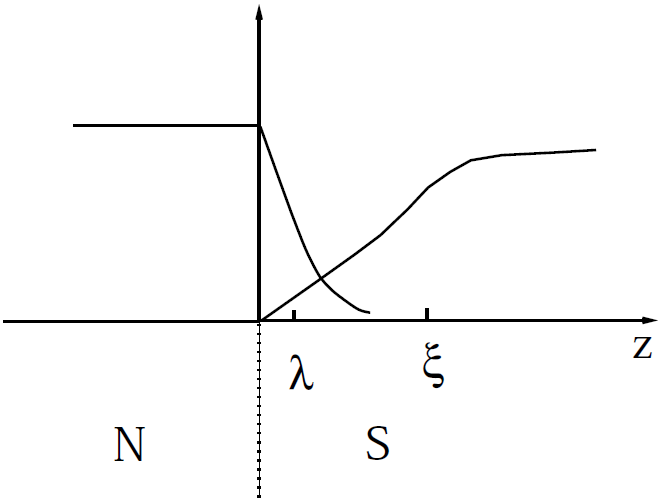
\includegraphics[width=0.45\textwidth]{immagini/GL_contributi_energetici.png}};
        % Rende disponibili le coordinate normalizzate (0..1, 0..1) sull'immagine
        \begin{scope}[x={(img.south east)}, y={(img.north west)}]
            % Esempi di disegni sopra:
            \node at (0.05,0.75) {$\dfrac{H}{H_c}$};
            \node[right] at (0.9,0.71) {$\dfrac{\psi(x)}{\psi_\infty}$};
        \end{scope}
    \end{tikzpicture}
\end{figure}
\hspace{-0.6cm}Stiamo integrando tra $-\infty$ e $+\infty$, quindi consideriamo sia la regione normale sia quella superconduttiva.\\
Nella regione normale sappiamo che il campo applicato è diverso da zero, quindi $\frac{H}{H_c}=1$, poiché siamo al campo critico.\\
Sappiamo però che il campo magnetico decade progressivamente all'interno del superconduttore, per cui all'interno di quest'ultimo assume un andamento come quello mostrato, con una scala caratteristica pari a $\lambda$.\\
L'altro contributo è quello del parametro d'ordine, che è nullo nella fase normale e diverso da zero nella fase superconduttiva. In particolare, esso tende al valore asintotico lontano dall'interfaccia e decade verso zero vicino all'interfaccia con una scala caratteristica $\xi$.\\
Vediamo ora il segno dell'energia.
\begin{figure}[H]
   \centering
   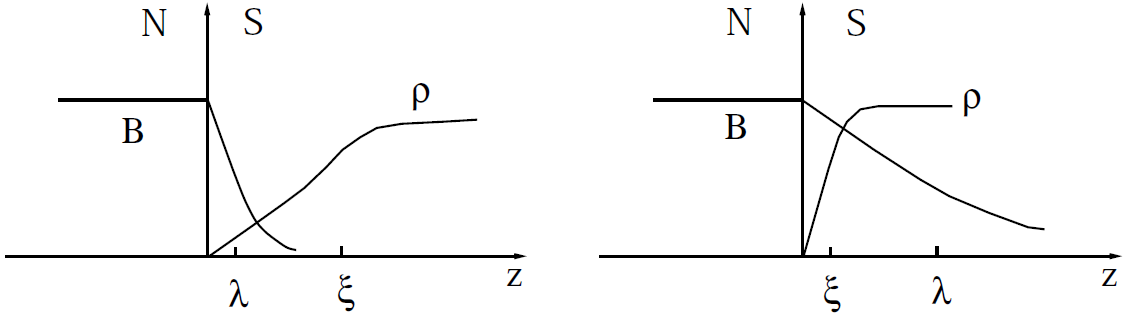
\includegraphics[width=0.8\textwidth]{immagini/energia_superficiale_superconduttore_tipo_I_e_II.png}
\end{figure}
\hspace{-0.6cm}Distinguiamo i due casi:
\begin{itemize}[leftmargin=0.5cm]
   \item Il caso $\kappa \ll 1$, cioè $\lambda \ll \xi$, è rappresentato a sinistra. In tale situazione si ottiene un'energia positiva. Ciò significa che non è conveniente avere molte superfici che separano le due fasi. Si ottiene quindi il comportamento tipico dei superconduttori di tipo I, nei quali compare essenzialmente un'unica superficie di separazione.
   \item Il caso opposto, $\kappa \gg 1$, cioè $\lambda \gg \xi$, è rappresentato a destra. In tale situazione il campo magnetico penetra profondamente nel materiale mentre il parametro d'ordine decade rapidamente vicino alla superficie. In questo caso abbiamo i superconduttori di tipo II. Qui è energeticamente conveniente avere molte superfici di separazione, e il campo penetra sotto forma di vortici.
\end{itemize}
Vediamo qualitativamente perché l'energia è positiva in un caso e negativa nell'altro:
\begin{figure}[H]
   \centering
   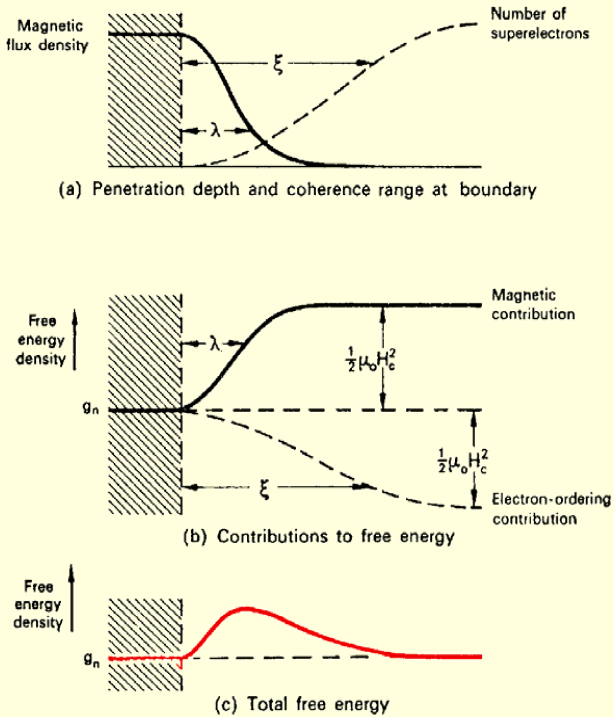
\includegraphics[width=0.45\textwidth]{immagini/energia_superficiale_positiva.png}
   \hspace{0.5cm}
   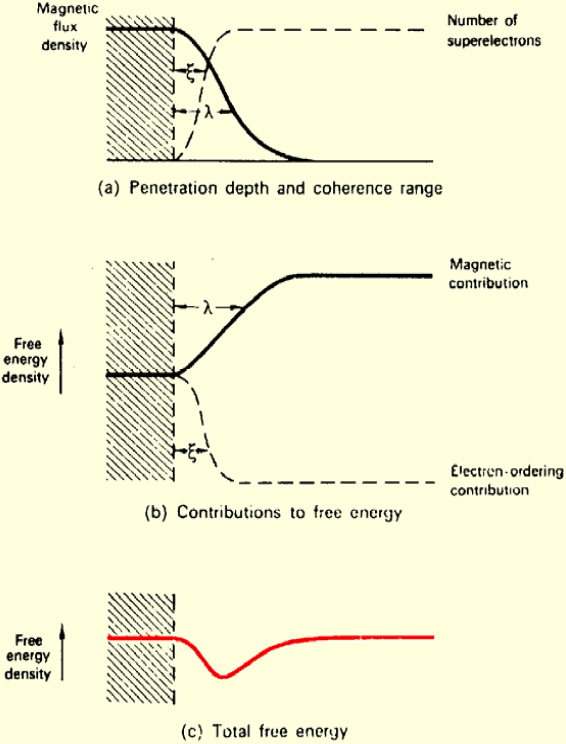
\includegraphics[width=0.45\textwidth]{immagini/energia_superficiale_negativa.png}
\end{figure}
\hspace{-0.6cm}Nel grafico sono mostrati i contributi all'energia libera superficiale, cioè i due termini che compaiono nell'integrale dell'\eqrefcustom{eq:contributo_superficiale_finale}.\\
Consideriamo dapprima il contributo magnetico, cioè $\qty(1-h/H_c)^2$. Avvicinandoci alla superficie, sappiamo che $h$ tende al campo applicato. Di conseguenza il termine $1-h/H_c$ parte da zero. Lontano dall'interfaccia, invece, $h\to 0$, quindi il termine tende a $1$.\\
Tra questi due limiti abbiamo un andamento continuo.\\
Consideriamo ora il contributo legato a $\psi$, $\abs{\psi/\psi_\infty}^4,$ che entra con segno negativo.\\
Vicino all'interfaccia siamo prossimi alla fase normale, quindi $\psi=0$ e il termine parte anch'esso da zero.\\
Per $x \to +\infty$, invece, $\psi \to \psi_\infty$, quindi il rapporto tende a $1$, ma compare con segno negativo nell'energia. Il contributo totale all'integrale è quindi negativo e ha un andamento come quello mostrato nel grafico.\\
Osserviamo che se $\lambda<\xi$, nel momento in cui sommiamo i due termini ci sarà una regione spaziale in cui il contributo totale resta positivo, e questo perché in tale regione il contributo associato al campo magnetico è maggiore del valore assoluto del contributo associato al parametro d'ordine, per cui prevale. In definitiva, in questo caso otteniamo un'energia superficiale che risulta positiva, tendendo a zero per $x\to 0 $ e per $x \to +\infty$.\\
Nel caso opposto, in cui $\xi \ll \lambda$, le scale spaziali si invertono, per cui il contributo negativo associato al parametro d'ordine prevale e la differenza tra i due termini diventa negativa. In questo caso avremo quindi un comportamento per l'energia superficiale tale per cui agli estremi tende ancora ad annullarsi, ma nel mezzo è sempre negativa.\\
Questo spiega perché, a seconda del rapporto tra profondità di penetrazione e lunghezza di coerenza, il costo energetico della superficie possa risultare positivo oppure negativo.\\
Per la maggior parte dei superconduttori elementari vale $\kappa<1$, quindi essi sono superconduttori di tipo I. Nei composti più complessi invece $\kappa$ è tipicamente molto maggiore di uno e il materiale appartiene alla classe dei superconduttori di tipo II.\\
Riassumendo:
\begin{itemize}[leftmargin=0.5cm]
   \item se $\xi>\lambda$, il sistema minimizza il numero di superfici tra fase normale e superconduttiva: questo corrisponde ai superconduttori di tipo I;
   \item se $\lambda>\xi$, il sistema preferisce avere molte regioni normali separate da fase superconduttiva: questo porta ai vortici dei superconduttori di tipo II.
\end{itemize}
Questa descrizione qualitativa emerge dalla teoria di Ginzburg--Landau.\\
La teoria quantitativa della transizione tra le due classi di superconduttori fu sviluppata da Abrikosov, che ricevette il premio Nobel nel 2003 insieme a Ginzburg e Leggett.\\
In quella teoria venne mostrato che il valore critico che separa i due comportamenti è
\begin{equation*}
   \kappa_c
   =
   \frac{1}{\sqrt{2}}
\end{equation*}
Inoltre fu possibile dimostrare che i vortici non si distribuiscono casualmente nel materiali, bensì esiste una configurazione di minima energia in cui i vortici formano un reticolo regolare. In particolare, il reticolo di vortici, detto reticolo di Abrikosov, è un reticolo triangolare, come mostrato nella figura seguente:
\begin{figure}[H]
   \centering
   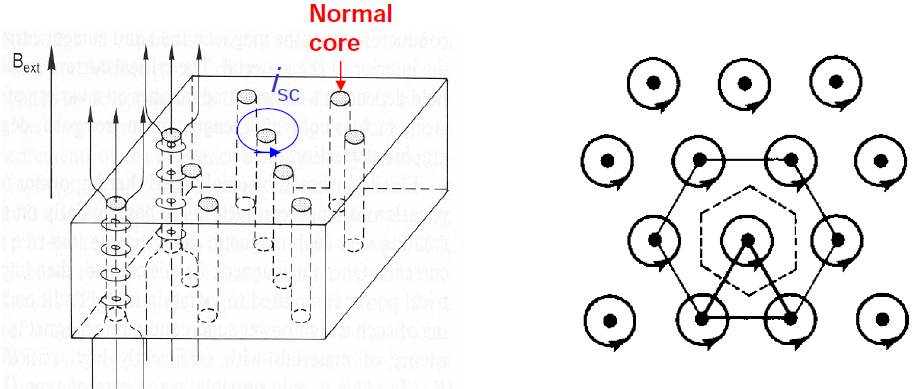
\includegraphics[width=0.7\textwidth]{immagini/Abrikosov_flux_Lattice.png}
\end{figure}
\hspace{-0.6cm}Questa è la tipica struttura della penetrazione del campo magnetico in un superconduttore di tipo II: abbiamo dei nuclei normali nei quali penetra il campo magnetico, i quali sono circondati da supercorrenti. Il comportamento è coerente con quanto già visto nella teoria di London, ma qui derivato in modo più accurato.\\
Fu inoltre possibile mostrare che i vortici non possono trasportare un flusso arbitrario. In altre parole, il flusso magnetico attraverso ciascun vortice può assumere soltanto valori pari a multipli interi del quanto di flusso $\Phi_0$, che è un fenomeno puramente quantistico.\\
La teoria permette anche di studiare l'interazione tra vortici, in particolare essi tendono a respingersi. Inoltre, se nel materiale sono presenti impurità, esse
tendono a rendere il materiale in loro prossimità in fase normale. Ciò significa che tipicamente i vortici tendono a localizzarsi in corrispondenza di queste impurità.\\
Osserviamo infine l'andamento della magnetizzazione in funzione del campo applicato nel caso dei superconduttori di tipo I e di tipo II:
\begin{figure}[H]
   \centering
   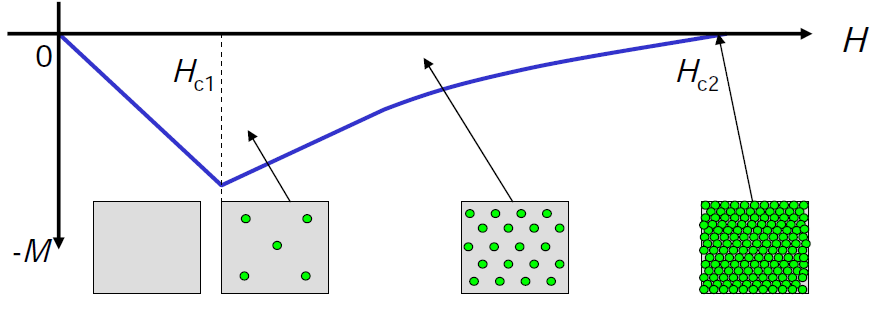
\includegraphics[width=0.8\textwidth]{immagini/andamento_magnetizzazione_superconduttore_tipo_I_e_II.png}
\end{figure}
\hspace{-0.6cm}Abbiamo già visto che in un superconduttore di tipo I si osserva il tipico comportamento diamagnetico fino al campo critico $H_c$.\\
In un superconduttore di tipo II, invece, compare una prima regione fino a un certo $H_{c,1}$ in cui il comportamento è identico a quello di un superconduttore di tipo I. Abbiamo poi una regione intermedia tra $H_{c,1}$ e $H_{c,2}$ in cui il campo penetra sotto forma di vortici, rappresentati nel grafico dai cerchi verdi. Notiamo come all'aumentare del campo magnetico, il numero di vortici aumenta e la loro densità diventa sempre più elevata, fino a riempire completamente il materiale in prossimità di $H_{c,2}$. Ciò non è altro che il materiale in fase normale per campi superiori a $H_{c,2}$.
\subsection{Stati intermedi nei superconduttori di tipo I}
Vediamo più nel dettaglio cosa accade nei superconduttori di tipo I.\\
Finora, quando abbiamo studiato ciò che accade in prossimità della superficie che separa la fase normale da quella superconduttiva (oppure il vuoto dalla fase superconduttiva) abbiamo considerato una geometria molto semplice. In particolare, abbiamo considerato la situazione in cui si applica un campo magnetico parallelo alla superficie di separazione tra il semispazio vuoto e il semispazio superconduttivo.\\
In realtà, le cose sono un po' più complicate se la superficie del materiale non ha una geometria così semplice, ma possiede invece una forma arbitraria. In questo caso la situazione non è così immediata, perché può verificarsi una penetrazione del campo magnetico anche nei superconduttori di tipo I.\\
In altre parole, in geometrie più complesse rispetto a quella discussa finora, possiamo avere la coesistenza di fasi normali e superconduttive, pur restando in una situazione completamente diversa dalla fase a vortici dei superconduttori di tipo II.\\
L'esempio più semplice è il caso di un superconduttore di forma sferica immerso in una regione in cui è presente un campo magnetico applicato $H_a$:
\begin{figure}[H]
   \centering
   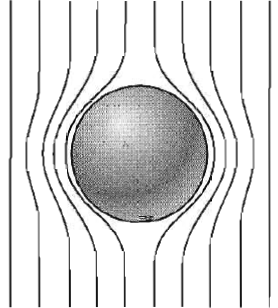
\includegraphics[width=0.25\textwidth]{immagini/sfera_superconduttiva.png}
\end{figure}
\hspace{-0.6cm}Lontano dalla sfera, il campo è uniforme e orientato lungo una certa direzione.\\
Avvicinandosi però al materiale superconduttivo, a causa dell'effetto Meissner il campo magnetico viene espulso. Questo implica che le linee di campo vicino alla superficie si deformano, assumendo una configurazione  tale che in prossimità del piano equatoriale le linee di campo diventano sempre più fitte.\\
Questo significa che il campo magnetico vicino alla superficie, in particolare nella regione equatoriale, aumenta di intensità, perché una maggiore densità di linee di campo corrisponde a un campo magnetico più intenso.\\
Risolvendo le equazioni di Maxwell si può mostrare che, vicino al piano equatoriale, il campo tangenziale alla superficie assume il valore
\begin{equation*}
   H_t=\frac{3}{2}H_a
\end{equation*}
Questo significa che, anche se applichiamo un campo magnetico $H_a$ minore del campo critico $H_c$, la situazione reale non è così semplice come ci si potrebbe aspettare intuitivamente.\\
Infatti, ingenuamente potremmo pensare che, finché $H_a < H_c$ il campo magnetico venga completamente espulso dal materiale. Tuttavia, il punto fondamentale è che il campo effettivamente percepito dalla superficie del materiale — in particolare vicino al piano equatoriale — non è $H_a$, bensì $\frac{3}{2}H_a$. Di conseguenza, il materiale può trovarsi localmente in condizioni tali da permettere la penetrazione del campo magnetico anche se il campo applicato lontano dal campione è ancora minore di $H_c$.\\
In particolare, se il campo applicato soddisfa
\begin{equation*}
   \frac{2}{3}H_c < H_a < H_c
\end{equation*}
si avrà la coesistenza di fase normale e fase superconduttiva all'interno del materiale.\\
Questo esempio riguarda il caso sferico, ma fenomeni analoghi si verificano anche per materiali con forme differenti.\\
Si introduce allora il cosiddetto fattore di demagnetizzazione $\eta$, definito in modo tale che, quando il campo applicato soddisfa
\begin{equation*}
   1-\eta < \frac{H_a}{H_c} < 1
\end{equation*}
si ha la coesistenza delle fasi normale e superconduttiva, cioè una penetrazione parziale del campo magnetico nel materiale.\\
In altre parole, $\eta$ quantifica quanto il campo magnetico applicato possa penetrare nel materiale anche se il valore del campo esterno è inferiore a $H_c$, che sarebbe invece il valore critico nel caso semplice di un campo parallelo alla superficie.\\
A questo punto ci chiediamo come penetri nel materiale il campo magnetico in queste condizioni. Supponiamo di avere un materiale cilindrico:
\begin{figure}[H]
   \centering
   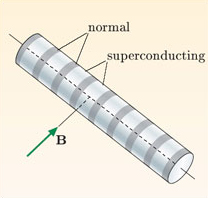
\includegraphics[width=0.4\textwidth]{immagini/cilindro_superconduttivo.png}
\end{figure}
\hspace{-0.6cm}Si può mostrare che se il campo magnetico è parallelo all'asse del cilindro, il comportamento è analogo a quello già visto nel caso di una lastra piana: il campo penetra soltanto entro una profondità dell'ordine di $\lambda$; se invece il campo magnetico è perpendicolare all'asse del cilindro, la situazione cambia completamente. In quest'ultimo caso si ha una deformazione delle linee di campo analoga a quella discussa per la sfera.\\
Di conseguenza, può verificarsi una penetrazione parziale del campo magnetico anche per valori di $B$ minori di $H_c$.\\
Si può mostrare che il campo penetra sotto forma di regioni laminate alternate, quindi avremo un'alternanza di lamelle normali e superconduttive. La penetrazione del campo avviene quindi in maniera laminare e non tramite vortici.\\
Come si osserva sperimentalmente questo fenomeno?\\
Se il sistema è immerso in un campo magnetico orientato perpendicolarmente all'asse del cilindro, il materiale diventa superconduttivo e presenta resistenza nulla per correnti che scorrono perpendicolarmente all'asse del cilindro.\\
Tuttavia, poiché il campo penetra tramite strati alternati normali e superconduttivi, una corrente che scorra lungo l'asse attraverserà un alternarsi di regioni a resistenza nulla e poi resistive. Di conseguenza il trasporto lungo questa direzione risulterà dissipativo.\\
Se invece consideriamo una corrente che fluisce perpendicolarmente all'asse del cilindro, il contributo delle regioni superconduttive prevale e il sistema si comporterà prevalentemente come un superconduttore, senza manifestare una resistenza apprezzabile.\\
Un comportamento analogo si osserva anche in una geometria a lastra piana:
\begin{figure}[H]
   \centering
   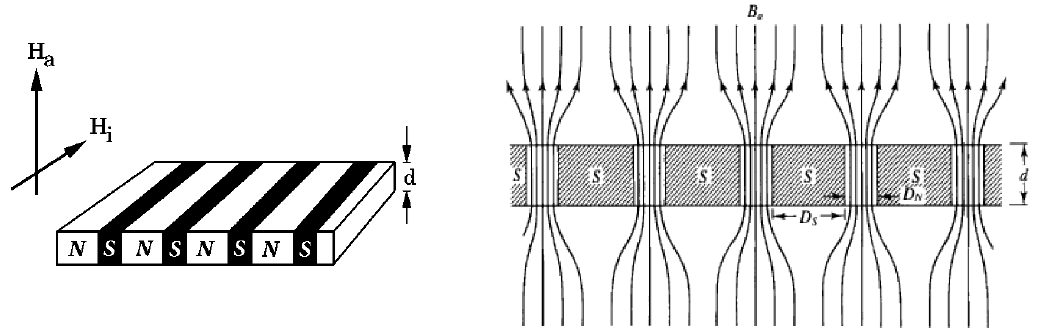
\includegraphics[width=0.9\textwidth]{immagini/lastra_superconduttiva.png}
\end{figure}
\hspace{-0.6cm}Se il campo magnetico è applicato perpendicolarmente alla lastra, la soluzione delle equazioni di Ginzburg--Landau o di London mostra ancora una volta che il campo penetra tramite un'alternanza di regioni normali e superconduttive.\\
Questo comportamento potrebbe ricordare quello dei vortici nei superconduttori di tipo II, ma in realtà si tratta di un fenomeno completamente diverso. La differenza fondamentale è che in questo caso le regioni normali in cui il campo magnetico è diverso da zero sono macroscopiche. Di conseguenza, il flusso magnetico che attraversa tali regioni non è quantizzato, cioè non è un multiplo intero del quanto di flusso $\Phi_0$. Inoltre, se osserviamo la lastra dall'alto, vediamo chiaramente l'alternanza di strisce normali e superconduttive.\\
Questo tipo di penetrazione prende il nome di penetrazione laminare.\\
Il messaggio fondamentale è quindi il seguente:
\begin{itemize}[leftmargin=0.5cm]
   \item anche nei superconduttori di tipo I il campo magnetico può penetrare nel materiale;
   \item ciò può dare origine alla coesistenza di regioni normali e superconduttive;
   \item la penetrazione avviene però tramite domini normali macroscopici e non tramite vortici quantizzati;
   \item il fenomeno dipende fortemente dalla geometria del campione e dalla direzione del campo magnetico rispetto alla superficie.
\end{itemize}
\subsection{Effetto di prossimità}
L'effetto di prossimità è un fenomeno che si verifica in generale tra due metalli quando almeno uno dei due è superconduttore. L'altro può trovarsi nella fase normale oppure entrambi possono essere materiali superconduttivi caratterizzati però da differenti temperature critiche, $T_{c,A}$ e $T_{c,B}$, con $T_{c,A}>T_{c,B}$.\\
Supponiamo di avere l'interfaccia tra questi due superconduttori. Se eseguiamo un esperimento abbassando progressivamente la temperatura, il materiale con temperatura critica maggiore diventerà superconduttivo per primo, mentre l'altro si troverà ancora nella fase normale.\\
Quando esiste una superficie che separa i due materiali, il materiale con temperatura critica più alta può "indurre" la superconduttività nel materiale vicino. Questo fenomeno prende il nome di effetto di prossimità.\\
Ciò significa che gli elettroni del materiale posto a contatto con il superconduttore a temperatura critica più alta possono anch'essi entrare nella fase superconduttiva. Questo accade anche se la temperatura del materiale $B$ è ancora maggiore della sua temperatura critica intrinseca.\\
Dal punto di vista tecnologico questo effetto è particolarmente importante. Immaginiamo infatti di avere un materiale con temperatura critica sufficientemente alta e, nelle sue vicinanze, uno strato molto sottile di un altro materiale avente una temperatura critica molto più piccola di $T_{c,A}$.\\
Per portare quest'ultimo nella fase superconduttiva dovremmo normalmente abbassare notevolmente la temperatura. Tuttavia, se lo strato viene posto sufficientemente vicino al materiale con temperatura critica più alta, esso può diventare superconduttivo proprio grazie all'effetto di prossimità.\\
In altre parole, il materiale può entrare nella fase superconduttiva pur trovandosi a una temperatura maggiore della sua temperatura critica intrinseca.\\
Questo è il fenomeno che si osserva, ad esempio, in geometrie nelle quali abbiamo un superconduttore da un lato e un altro superconduttore dall'altro lato — supponiamo identici, quindi entrambi caratterizzati dalla stessa temperatura critica $T_{c,B}$ — separati da uno strato estremamente sottile di un altro materiale.\\
Nel limite più estremo questo strato può avere lo spessore di un singolo atomo. È proprio ciò che accade tipicamente nel caso del grafene, che sarà oggetto dell'ultima parte del corso.\\
Il grafene è essenzialmente un materiale bidimensionale: il suo spessore nella direzione perpendicolare al piano è dell'ordine di un singolo strato atomico.\\
Essendo costituito da carbonio, il grafene è normalmente un metallo con una particolare struttura a bande. Il suo spettro elettronico differisce da quello di un metallo convenzionale.\\
Quando però inseriamo questo sottilissimo strato di grafene tra due superconduttori, si manifesta proprio l'effetto di prossimità.\\
Ciò significa che può fluire una supercorrente tra i due superconduttori attraversando lo strato bidimensionale di grafene.\\
In questo caso otteniamo una giunzione superconduttiva nella quale compare il cosiddetto effetto Josephson attraverso uno strato di grafene: una graphene Josephson junction.\\
Nel corso parleremo più avanti delle giunzioni Josephson. Nel nostro caso esse saranno costituite da due superconduttori separati da uno strato isolante oppure da uno strato di materiale conduttivo. Vedremo che anche in quel caso può fluire una supercorrente. In generale il meccanismo sarà diverso dall'effetto di prossimità discusso qui.
\subsection{Quantizzazione del flusso}
Vediamo quali sono le implicazioni della teoria di Ginzburg--Landau per quanto riguarda la connessione tra campo magnetico e differenti geometrie del superconduttore. Questo ci porterà alla quantizzazione del flusso. Inoltre, analizzeremo anche la natura della transizione che avviene nel passaggio dalla fase normale alla fase superconduttiva e, in particolare, quale simmetria venga rotta durante questa transizione.\\
L'idea è capire che cosa accade al campo magnetico quando abbiamo un materiale superconduttivo e partiamo dalla descrizione in termini del parametro d'ordine complesso. Vedremo infatti che tutti questi fenomeni sono profondamente legati proprio alla natura complessa del parametro d'ordine.\\
Il parametro d'ordine $\psi(\vb{r})$ deve essere una funzione ad un sol valore. Questo significa che l'integrale lungo una linea chiusa del gradiente della fase $\phi$ deve essere pari a un multiplo intero di $2\pi$:
\begin{equation}
    \oint \grad{\phi} \vdot \dd{\vb{s}}
    =
    2\pi n
    \label{eq:integrale_phi_curva_chiusa}
\end{equation}
Vediamo quali implicazioni abbia questa proprietà sulla densità di supercorrente, che abbiamo già visto poter essere espressa tramite l'\eqrefcustom{eq:densita_di_supercorrente}, con $|\psi|^2$ che identifica la densità di elettroni superconduttivi $n_s$.\\
Da questa identità possiamo anche scrivere il momento quantistico nella forma
\begin{equation*}
    m^*\vb{v}_s
    =
    \hbar \grad{\phi}
    -
    \frac{e^*}{c}\vb{A}.
\end{equation*}
Poiché deve valere la \eqref{eq:integrale_phi_curva_chiusa}, deve risultare
\begin{equation}
   \oint \qty[ m^* \vb{v}_s + \frac{e^*}{c}\vb{A} ] \vdot \dd{\vb{s}}
   =\hbar 2\pi n
   \label{eq:integrale_momento_curva_chiusa}
\end{equation}
Cioè, se integriamo lungo una linea chiusa questa combinazione di termini — che corrisponde a $\grad{\phi}$ — dobbiamo ottenere $\hbar 2\pi n$.\\
Osserviamo ora che l'integrale del potenziale vettore è in realtà uguale al flusso del campo magnetico, purché la linea e la superficie siano legate dalla condizione che la prima sia il bordo della seconda:
\begin{equation}
   \oint \vb{A}\vdot\dd{\vb{s}}
   =
   \int_{\Sigma}\vb{h}\vdot\dd{\vb*{\Sigma}}
   \label{eq:integrale_A_flusso_B}
\end{equation}
dove abbiamo usato $\vb{h}$ invece di $\vb{B}$ perché intendiamo il campo magnetico locale.\\
Possiamo quindi riscrivere la relazione precedente esprimendo l'integrale di linea di $\vb{A}$ in termini del flusso del campo magnetico. Moltiplicando per $c/e^*$ otteniamo
\begin{equation*}
    \int_{\Sigma}
    \vb{h}\vdot\dd{\vb*{\Sigma}}
    +
    \frac{c}{e^*}
    \oint
    m^*\vb{v}_s\vdot\dd{\vb{s}}
    =
    2\pi n\frac{c\hbar}{e^*}
    \equiv
    n\Phi_0
\end{equation*}
Il risultato che troviamo è una quantità avente le dimensioni di un flusso magnetico. Questo ci dice che la combinazione tra il flusso del campo magnetico in una geometria generica e il contributo associato al momento dei portatori deve essere uguale a un multiplo intero di una quantità che ha le dimensioni di flusso magnetico.\\
Questa condizione prende il nome di \emph{condizione di quantizzazione del flussoide} (\emph{fluxoid quantization condition}), dove il quanto di flussoide è
\begin{equation*}
   \Phi_0
   =
   2\pi\hbar\frac{c}{2e}
   =
   2.07\times10^{-7}\,\text{Gauss cm}^2,
\end{equation*}
avendo posto la carica efficace dei portatori pari a $2e$ (risultato che emerge rigorosamente dalla teoria BCS). Questa quantità è chiamata \emph{quanto di flusso}.\\
Vediamo ora quali siano le implicazioni di questa condizione nei diversi casi possibili:
\begin{itemize}[leftmargin=0.5cm]
   \item all'interno del bulk di un superconduttore;
   \item nel caso in cui esistano regioni normali all'interno del superconduttore;
   \item nel caso di un superconduttore con geometria ad anello.
\end{itemize}
Vedremo che, a seconda della situazione, questa relazione conduce a conseguenze differenti.\\[0.2cm]
\textbf{Primo caso: bulk completamente superconduttivo}\\
Supponiamo di avere un materiale bulk interamente nella fase superconduttiva, senza alcuna regione normale interna, e consideriamo un contorno chiuso all'interno del materiale.
\begin{figure}[H]
   \centering
   \begin{tikzpicture}[scale=1.5]
      % Cerchio interno
      \begin{scope}[canvas is xz plane at y=0]
         \draw[thick, red, opacity=0.75] (1.6,0.5) circle (0.8);
      \end{scope}
      % Faccia frontale semi-trasparente, sopra il cerchio
      \draw[ fill=gray!40, fill opacity=0.65, draw=black] (0,0,0) -- (0,-1,0) -- (2,-1,0) -- (2,0,0) -- cycle;
      % Faccia superiore e laterale, dietro
      \draw[fill=gray!70, fill opacity=0.65, draw=black] (0,0,0) -- (0,0,-2) -- (2,0,-2) -- (2,0,0) -- cycle;
      \draw[fill=gray!55, fill opacity=0.65, draw=black] (2,0,0) -- (2,0,-2) -- (2,-1,-2) -- (2,-1,0) -- cycle;
   \end{tikzpicture}
\end{figure}
\hspace{-0.6cm}Poiché siamo nel bulk del superconduttore, per effetto Meissner sappiamo che il campo magnetico deve essere nullo. Ma se il campo magnetico è nullo nella parte interna del materiale, allora deve essere nulla anche la supercorrente, dato che essa scorre soltanto in prossimità della superficie.\\
In queste condizioni abbiamo quindi che $\vb{h}=0$ e $\vb{J}_s=0$. Da ciò segue che l'intero $n$ deve essere uguale a zero. Tornando allora all'\eqrefcustom{eq:integrale_phi_curva_chiusa}, otteniamo
\begin{equation*}
   \oint \grad{\phi} \vdot \dd{\vb{s}}=0
\end{equation*}
e ciò implica che la fase non può dipendere dalla posizione all'interno del bulk del superconduttore: la fase $\phi$ deve quindi essere uniforme.\\
Questa è un'osservazione molto importante, perché implica che nel bulk del superconduttore il parametro d'ordine può avere un modulo dipendente dalla posizione, ma il fattore di fase deve essere costante:
\begin{equation*}
      \psi(\vb{r})
      =
      |\psi(\vb{r})|e^{i\phi}
\end{equation*}
Vedremo che questo risultato è legato anche al tipo di simmetria che viene rotta durante la transizione superconduttiva.\\[0.2cm]
\textbf{Secondo caso: presenza di regioni normali}\\
Consideriamo ora il caso in cui siamo ancora all'interno del bulk di un materiale superconduttivo, ma siano presenti alcune regioni normali.\\
Supponiamo, ad esempio, di avere un vortice, cioè una regione nella quale il campo magnetico penetra all'interno del materiale.
\begin{figure}[H]
   \centering
   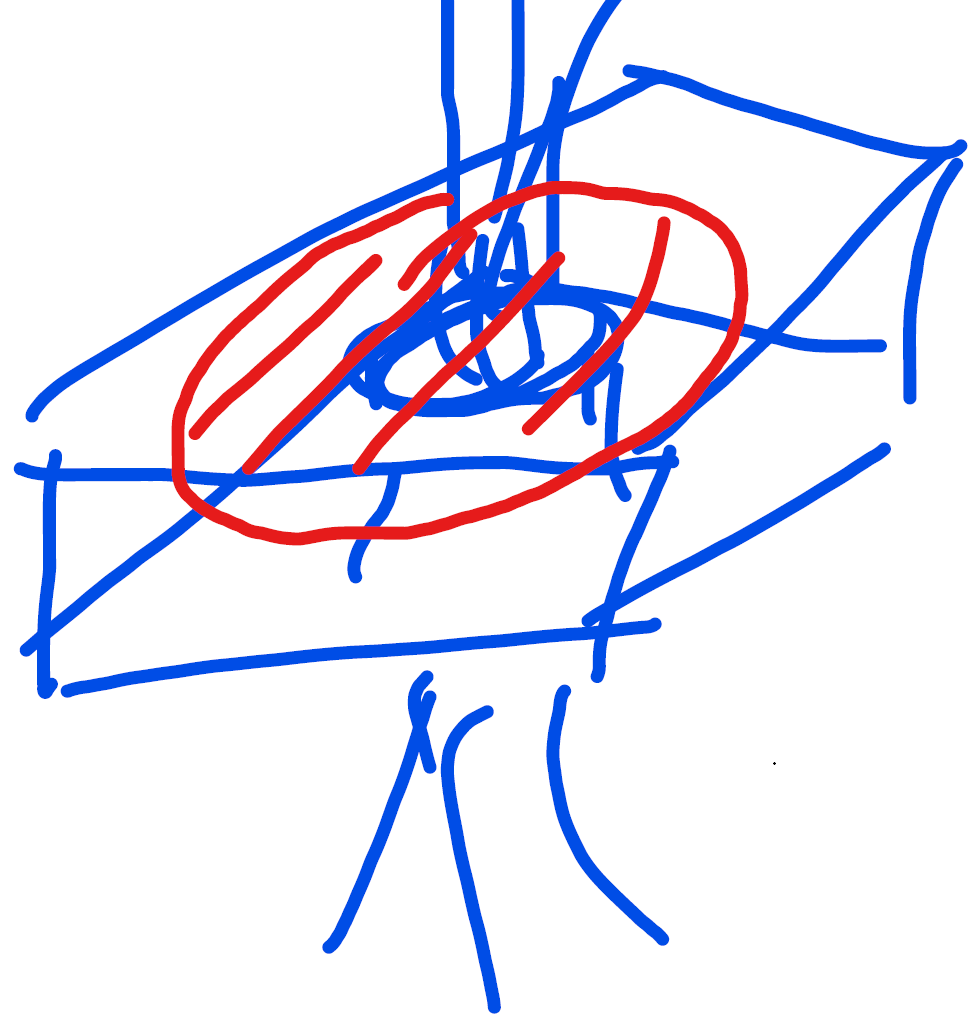
\includegraphics[width=0.3\textwidth]{immagini/fluxoid_quantization_vortice.png}
\end{figure}
\hspace{-0.6cm}Se scegliamo un contorno che circonda questa regione normale, ci troviamo ancora nella situazione in cui la densità superconduttiva è nulla lontano dalla superficie, quindi $\vb{J}_s=0$, ma il campo magnetico attraversa la superficie delimitata dal contorno.\\
In questo caso, l'\eqrefcustom{eq:integrale_momento_curva_chiusa} implica allora che il flusso del campo magnetico attraverso tale superficie deve essere uguale a un multiplo intero del quanto di flusso:
\begin{equation*}
   \int_{\Sigma} \vb{h}\vdot\dd{\vb*{\Sigma}}
   =2\pi n\frac{c\hbar}{e^*}
   \equiv n\Phi_0
\end{equation*}
Questa non è altro che la condizione che avevamo già menzionato parlando dei superconduttori di tipo II. Essa ci dice che il flusso magnetico che penetra nel superconduttore non può assumere valori arbitrari, ma deve essere quantizzato.\\
Per esempio, nel caso dei superconduttori di tipo II, dove il campo magnetico penetra nel materiale, i flussi $\Phi_1, \Phi_2, \ldots$ associati ai campi magnetici $h_1, h_2, \ldots$ non possono essere arbitrari. Essi devono necessariamente essere pari a $n_1\Phi_0, n_2\Phi_0, \dots$, cioè a multipli interi del quanto di flusso.\\[0.2cm]
\textbf{Terzo caso: anello superconduttivo}\\
Consideriamo infine un anello superconduttivo.
\begin{figure}[H]
   \centering
   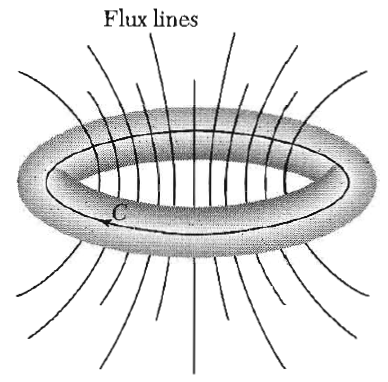
\includegraphics[width=0.4\textwidth]{immagini/fluxoid_quantization_anello.png}
\end{figure}
\hspace{-0.6cm}Supponiamo di prendere un contorno all'interno dell'anello come mostrato. In questo caso, nella parte interna del materiale superconduttivo abbiamo ancora $\vb{h}=0$ e $\vb{J}_s=0$, ma la superficie delimitata dal contorno racchiude una regione vuota nella quale il campo magnetico può penetrare. Di conseguenza, esiste un flusso magnetico non nullo attraverso tale superficie.\\
Anche in questo caso, la condizione di quantizzazione appena ottenuta implica che il flusso debba essere un multiplo intero del quanto di flusso.\\
Questo significa che, se raffreddiamo un anello superconduttivo in presenza di un campo magnetico, quando il sistema attraversa la transizione superconduttiva e successivamente il campo magnetico esterno viene spento, all'interno dell'anello rimane intrappolato un flusso magnetico quantizzato.\\
Ciò avviene perché continua a circolare una supercorrente lungo l'anello, la quale genera un campo magnetico che resta confinato all'interno della geometria ad anello.\\
La differenza rispetto al caso precedente è che qui stiamo considerando una struttura costruita artificialmente, mentre nel caso del bulk con vortici il sistema sviluppa spontaneamente regioni normali all'interno del materiale.\\
Il risultato fondamentale è comunque lo stesso, in quanto il flusso magnetico intrappolato nell'anello non è arbitrario, ma deve essere necessariamente uguale a un multiplo intero di $\Phi_0$, e ciò qualunque sia la grandezza dell'anello.\\
Per comprendere meglio il significato di questo risultato, proviamo ora a derivarlo dal punto di vista energetico.\\
Se il sistema si comporta in questo modo, significa che deve essere energeticamente conveniente trovarsi in una configurazione in cui il flusso magnetico è quantizzato.\\
Dobbiamo quindi partire dall'espressione dell'energia libera in una situazione di questo tipo e vedere quale forma assume.\\
Per farlo, descriviamo il sistema mediante coordinate polari cilindriche, $\vb{r} = (r,\varphi,z)$, con l'asse $z$ perpendicolare al piano dell'anello.\\ Supponiamo innanzitutto che le variazioni di $\psi(\vb{r})$ attraverso la sezione trasversale dell'anello siano trascurabili; possiamo quindi ignorare qualsiasi dipendenza da $r$ e $z$, dunque $\psi(\vb{r})=\psi(\varphi)$.\\ 
Inoltre, affinché il parametro d'ordine sia una funzione ad un solo valore, esso deve essere periodico nell'angolo $\varphi$:
\begin{equation}
   \psi(\varphi+2\pi)=\psi(\varphi)
   \label{eq:condizione_singolo_valore_psi}
\end{equation}
Ciò implica che la dipendenza funzionale di $\psi(\varphi)$ debba essere di tipo esponenziale:
\begin{equation*}
   \psi(\varphi)=\psi_0 e^{in\varphi}
\end{equation*}
dove $n$ rappresenta un numero di avvolgimenti.\\
Per rendere la trattazione il più semplice possibile, assumiamo inoltre che il campo magnetico sia uniforme all'interno dell'anello.\\
In queste condizioni esiste una relazione semplice tra l'integrale di linea del potenziale vettore e il flusso del campo magnetico. Possiamo infatti assumere che $\vb{A}$ sia costante lungo l'anello e quindi dall'\eqrefcustom{eq:integrale_A_flusso_B} segue
\begin{equation*}
   \Phi(\vb{B}) = A\,2\pi R
\end{equation*}
da cui
\begin{equation}
   \vb{A} = \frac{\Phi(\vb{B})}{2\pi R}\vu{u}_{\varphi}
   \label{eq:vector_potential_ring}
\end{equation}
Con queste ipotesi possiamo inserire le proprietà appena trovate nell'energia libera di Ginzburg--Landau.\\
Abbiamo visto che l'energia libera della fase superconduttiva può essere scritta come somma dell'energia libera della fase normale e del contributo di Ginzburg--Landau:
\begin{equation*}
   \begin{split}
      F_s
      &=
      F_n
      +
      \int \dd[3]{\vb{r}}
      \qty{
      \frac{\hbar^2}{2m^*}
      \qty|
      \qty(
         \grad
         +
         i\frac{2e}{c\hbar}\vb{A}
      )\psi
      |^2
      +
      a|\psi|^2
      +
      \frac{b}{4}|\psi|^4
      }
      +
      E_B
      \\
      &=
      F_s^0
      +
      \int \dd[3]{\vb{r}}
      \qty{
      \frac{\hbar^2}{2m^*}
      \qty|
      \qty(
         \grad
         +
         i\frac{2e}{c\hbar}\vb{A}
      )\psi
      |^2
      }
      +
      E_B
   \end{split}
\end{equation*}
dove
\begin{equation*}
   F_s^0
   =
   F_n
   +
   \int \dd[3]{\vb{r}}
   \qty{
   a|\psi|^2
   +
   \frac{b}{4}|\psi|^4
   }
\end{equation*}
è l'energia libera dello stato fondamentale dell'anello in assenza di correnti e di flussi magnetici, mentre $E_B$ rappresenta il contributo energetico del campo magnetico.\\
Usando ora l'\eqrefcustom{eq:condizione_singolo_valore_psi} e l'\eqrefcustom{eq:vector_potential_ring}, otteniamo\mn{Ricordiamo che dobbiamo usare il gradiente in coordinate cilindriche, ma avendo dipendenza soltanto da $\varphi$, esso diventa semplicemente
\begin{equation*}
   \grad=\frac{1}{r}\partial_\varphi \vu{u}_\varphi
\end{equation*}}
\begin{equation*}
   \qty(
      \grad
      +
      i\frac{2e}{c\hbar}\vb{A}
   )\psi
   =
   \qty(
      -i\frac{n}{R}
      +
      i\frac{2e}{c\hbar}
      \frac{\Phi(\vb{B})}{2\pi R}
   )
   \psi\vu{u}_\varphi.
\end{equation*}
Segue quindi che
\begin{equation*}
   \frac{\hbar^2}{2m^*}
   \qty|
   \qty(
      \grad
      +
      i\frac{2e}{c\hbar}\vb{A}
   )\psi
   |^2
   =
   \frac{\hbar^2}{2m^*R^2}
   \qty[
      n-\frac{\Phi(\vb{B})}{\Phi_0}
   ]^2
   |\psi|^2,
\end{equation*}
dove $\Phi_0=\frac{hc}{2e}$.\\
Integrando sul volume dell'anello otteniamo
\begin{equation*}
   \int \dd[3]{\vb{r}}
   \qty{
   \frac{\hbar^2}{2m^*}
   \qty|
   \qty(
      \grad
      +
      i\frac{2e}{c\hbar}\vb{A}
   )\psi
   |^2
   }
   =
   V
   \frac{\hbar^2}{2m^*R^2}
   \qty[
      n-\frac{\Phi(\vb{B})}{\Phi_0}
   ]^2
   |\psi|^2
\end{equation*}
Ricordiamo ora che conosciamo anche l'espressione del contributo energetico del campo magnetico. Infatti, poiché l'energia del campo magnetico è data dall'integrale sul volume interno all'anello, abbiamo
\begin{equation*}
   E_B
   =
   \int\displaylimits_{
      \begin{subarray}{c}
         \text{parte}\\
         \text{interna}
      \end{subarray}
   }
   \dd[3]{\vb{r}}
   \frac{B^2}{8\pi}
\end{equation*}
Questa espressione può essere riscritta in termini dell'autoinduttanza dell'anello:
\begin{equation*}
   E_B=\frac{1}{2}LI^2
\end{equation*}
Scrivendo il flusso magnetico nella forma $\Phi(\vb{B})=LI$, si ottiene infine
\begin{equation*}
   E_B = \frac{1}{2}\frac{\Phi^2}{L}
\end{equation*}
In conclusione, otteniamo
\begin{equation*}
   F_s
   =
   F_s^{\rm bulk}
   +
   \text{const.}
   \times
   \qty[
      n-\frac{\Phi(\vb{B})}{\Phi_0}
   ]^2
   |\psi|^2
   +
   \frac{1}{2}\frac{\Phi^2}{L}
\end{equation*}
Possiamo ora rappresentare queste energie in funzione del flusso $\Phi$:
\begin{figure}[H]
   \centering
   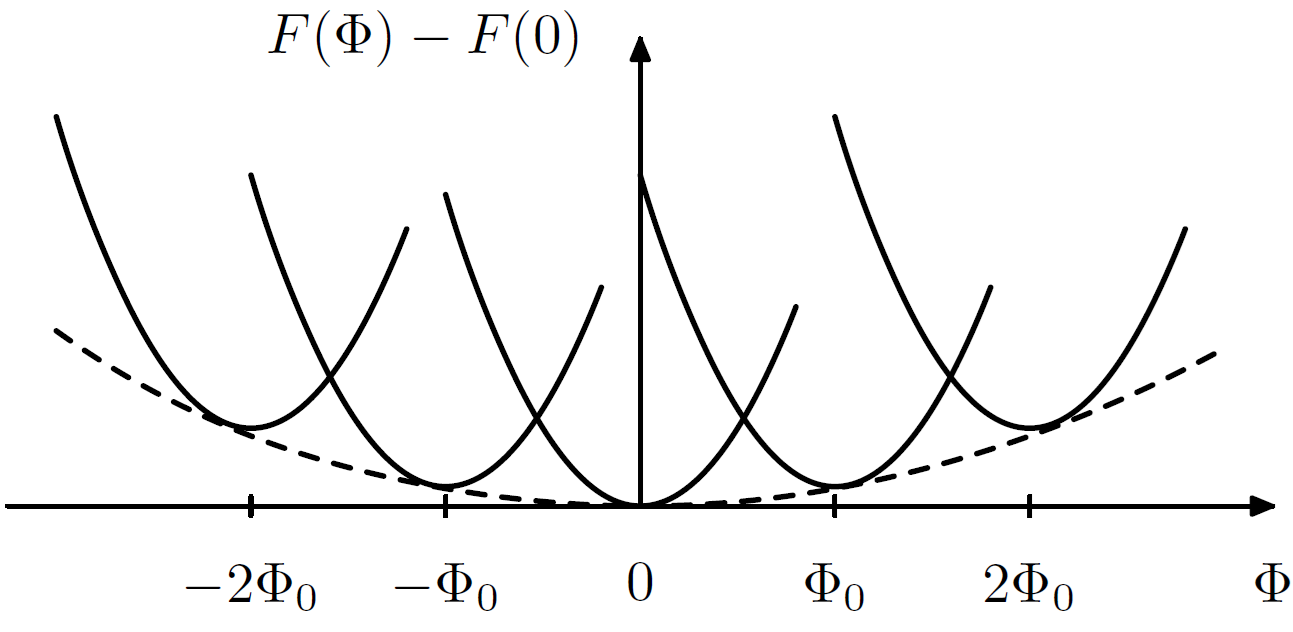
\includegraphics[width=0.6\textwidth]{immagini/energy_flux_quantization.png}
\end{figure}
\hspace{-0.6cm}Abbiamo la somma di due contributi: un termine puramente parabolico (rappresentato dalla linea tratteggiata) e una famiglia di parabole dipendenti da $n$. I minimi di tali parabole si trovano in corrispondenza della condizione
\begin{equation*}
   \frac{\Phi(\vb{B})}{\Phi_0}=n
\end{equation*}
quindi, per esempio, per $n=0$ la parabola è centrata in $\Phi=0$; per $n=1$ la parabola è centrata in $\Phi=\Phi_0$ e così via.\\
In definitiva, l'energia totale, data dalla somma di questi contributi, presenta una serie di minimi metastabili e lo stato finale del sistema (uno di questi minimi) dipenderà dalla storia del campo magnetico applicato. Per esempio, se il flusso iniziale è vicino a $\Phi_0$, il sistema rilasserà verso il minimo più vicino, cioè verso il minimo per $n=1$. In generale, la configurazione stabile sarà quella corrispondente al minimo energetico più vicino alla condizione iniziale.\\
Possiamo ora aggiungere un ulteriore ingrediente alla descrizione, che sarà rilevante nel seguito. Supponiamo di interpretare questa struttura come il paesaggio di energia potenziale visto da un sistema quantistico. In questo caso, abbiamo una serie di pozzi di potenziale separati da barriere.
\begin{figure}[H]
   \centering
   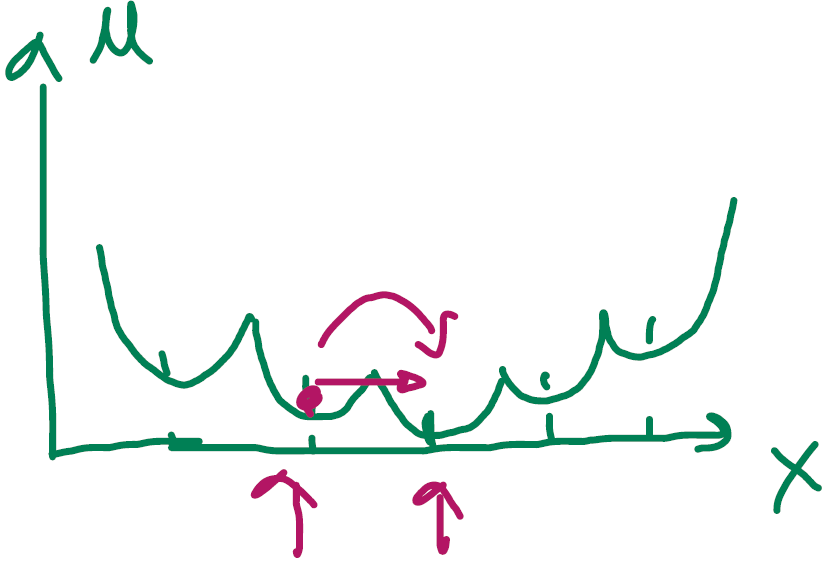
\includegraphics[width=0.5\textwidth]{immagini/energy_landscape_quantization.png}
\end{figure}
\hspace{-0.6cm}In meccanica quantistica, una particella descritta da una funzione d'onda può tunnelare da un minimo all'altro. Applicando questa idea al problema dell'anello superconduttivo, possiamo immaginare processi nei quali il sistema passa da un minimo metastabile al successivo tramite tunneling quantistico.\\
In termini della fase, ciò corrisponde al passaggio da $\phi$ a $\phi + 2\pi$, mentre dal punto di vista del numero di winding, ciò significa passare da $n$ a $n\pm1$.\\
Questi processi prendono il nome di \emph{phase slips}. Essi corrispondono quindi a cambiamenti discreti del numero di winding associati a processi di tunneling quantistico.\\
Poiché la supercorrente dipende da $n$, un cambiamento di $n$ implica anche una variazione della supercorrente che circola nell'anello.\\
Questi processi possono avvenire per tunneling quantistico a temperatura nulla oppure per attivazione termica a temperatura finita. A temperatura finita infatti gli stati eccitati sono popolati e possono attraversare più facilmente la barriera di potenziale oppure superarla termicamente.\\
In questo modo si hanno processi di decadimento della supercorrente.\\
L'aspetto più notevole è che, se facciamo un passo indietro e ricordiamo che il sistema è costituito da un enorme numero di elettroni, ci rendiamo conto che questi processi rappresentano tunneling quantistico macroscopico. Questo è alla base di fenomeni come il macroscopic quantum tunneling e la macroscopic quantum coherence, che verranno descritti in modo rigoroso dalla teoria BCS, nella quale introdurremo una vera funzione d'onda del condensato. Tuttavia, già nella teoria di Ginzburg--Landau emerge naturalmente una descrizione di questo tipo se interpretiamo il parametro d'ordine come una funzione d'onda macroscopica dell'intero sistema.\\
Naturalmente, manca ancora una giustificazione microscopica rigorosa, che verrà introdotta successivamente.\\
È comunque importante osservare quanto fosse profonda l'intuizione alla base della teoria di Ginzburg--Landau, in quanto essa riuscì a prevedere fenomeni estremamente non banali pur senza una teoria microscopica completa, utilizzando soltanto una descrizione fenomenologica basata sull'energia libera.\\
Consideriamo infine il seguente quadro qualitativo:
\begin{figure}[H]
   \centering
   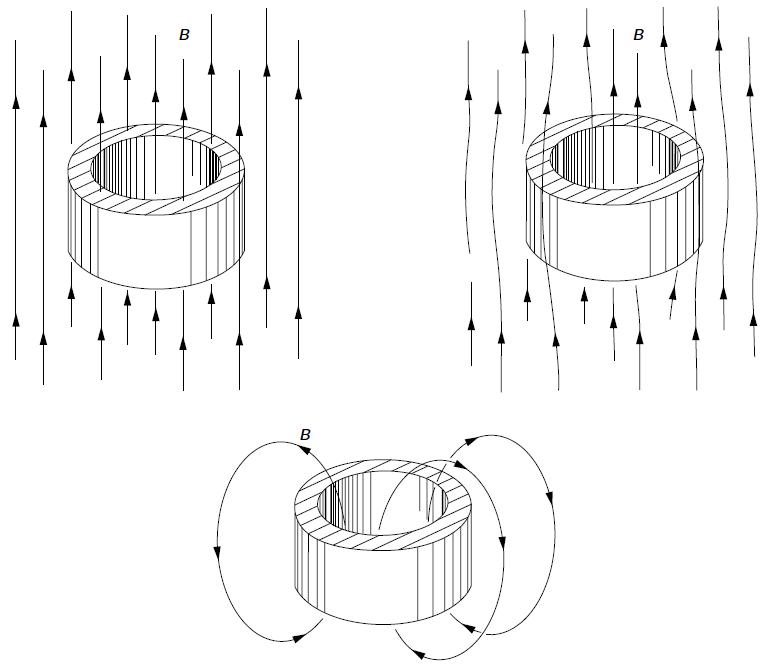
\includegraphics[width=0.7\textwidth]{immagini/flux_quantization_experiment.png}
\end{figure}
\hspace{-0.6cm}Partiamo da un anello superconduttivo nella fase normale immerso in un campo magnetico. Quando abbassiamo la temperatura al di sotto di $T_c$, il sistema entra nella fase superconduttiva e il campo magnetico viene espulso. Una parte del flusso resta intrappolata all'interno dell'anello e rimane confinato anche quando il campo magnetico esterno viene spento.\\
Il punto fondamentale è che il flusso intrappolato non può assumere valori arbitrari, ma solo multipli del quanto di flusso: $\Phi=n\Phi_0$.\\
Questo effetto fu misurato sperimentalmente nel 1961 da due gruppi differenti e rappresenta uno dei primi esempi di fenomeno quantistico macroscopico osservato sperimentalmente.
\subsection{Simmetria di gauge e rottura di simmetria}
Come abbiamo già visto, nella teoria di Ginzburg--Landau il parametro d'ordine è in generale una quantità complessa dipendente dalla posizione, nella forma dell'\eqrefcustom{eq:psi_con_fase}. Analizziamo ora cosa accade se eseguiamo una trasformazione di gauge.\\
Sappiamo che una trasformazione di gauge consiste nel trasformare il potenziale vettore in un nuovo potenziale vettore differente per il gradiente di una funzione scalare:
\begin{equation*}
   \vb{A} \to \vb{A} + \grad{\chi(\vb{r})}
\end{equation*}
Quello che stiamo per vedere è che, affinché la teoria soddisfi l'invarianza di gauge, questa trasformazione deve essere accompagnata anche da una trasformazione della fase del parametro d'ordine:
\begin{equation*}
   \psi(\vb{r}) \to \tilde{\psi}(\vb{r}) = \psi(\vb{r})e^{i\theta(\vb{r})}
\end{equation*}
Supponiamo di effettuare una trasformazione di gauge e consideriamo cosa accade se, partendo da un parametro d'ordine $\psi(\vb{r})$, passiamo a $\tilde{\psi}(\vb{r})$, che differisce dal primo soltanto per un fattore di fase dipendente dalla posizione.\\
Quello che vogliamo capire è quale sia l'effetto di questa trasformazione sull'energia libera di Ginzburg--Landau e, naturalmente, ciò che conta è l'effetto sul momento gauge-invariante associato al nuovo parametro d'ordine.\\
La prima cosa da fare è quindi valutare l'azione del momento gauge-invariante su $\tilde{\psi}(\vb{r})$:
\begin{equation*}
   \hat{p}\tilde{\psi}(\vb{r})
   =
   \frac{\hbar}{i}\grad{\tilde{\psi}(\vb{r})}
   -
   \frac{e^*}{c}\vb{A}\tilde{\psi}(\vb{r})
\end{equation*}
Dobbiamo allora capire come si trasforma il gradiente di $\tilde{\psi}(\vb{r})$:
\begin{equation*}
   \grad{\tilde{\psi}(\vb{r})}
   =
   \grad{
      \qty[
         \psi(\vb{r})e^{i\theta(\vb{r})}
      ]
   }
   =
   e^{i\theta(\vb{r})}\grad{\psi(\vb{r})}
   +
   ie^{i\theta(\vb{r})}\psi(\vb{r})\grad{\theta(\vb{r})}
\end{equation*}
Di conseguenza, il momento $\hat{p}$ agente su $\tilde{\psi}(\vb{r})$ assume la forma
\begin{equation*}
   \begin{split}
      \hat{p}\tilde{\psi}(\vb{r})
      &=
      \frac{\hbar}{i}
      e^{i\theta(\vb{r})}
      \grad{\psi(\vb{r})}
      +
      \hbar
      e^{i\theta(\vb{r})}
      \psi(\vb{r})
      \grad{\theta(\vb{r})}
      -
      \frac{e^*}{c}
      \vb{A}
      e^{i\theta(\vb{r})}
      \psi(\vb{r})
      \\
      &=
      e^{i\theta(\vb{r})}
      \qty[
      \frac{\hbar}{i}\grad
      +
      \hbar\grad{\theta(\vb{r})}
      -
      \frac{e^*}{c}\vb{A}
      ]
      \psi(\vb{r}).
   \end{split}
\end{equation*}
Gli ultimi due termini tra parentesi quadre possono essere riscritti come
\begin{equation*}
   \hbar\grad{\theta(\vb{r})}
   -
   \frac{e^*}{c}\vb{A}
   =
   -
   \frac{e^*}{c}
   \qty[
      \vb{A}
      -
      \frac{\hbar c}{e^*}
      \grad{\theta(\vb{r})}
   ].
\end{equation*}
Questa espressione non è altro che una trasformazione di gauge del potenziale vettore, perché è nella forma $\vb{A} \to \vb{A} + \grad{\chi}$.\\
Il punto fondamentale è quindi che nella teoria di Ginzburg--Landau, affinché la teoria sia invariante per trasformazioni di gauge locali, è necessario trasformare simultaneamente: il potenziale vettore e la fase del parametro d'ordine. Dobbiamo cioè effettuare entrambe le trasformazioni per mantenere l'invarianza di gauge.\\
Questa invarianza è detta \emph{invarianza di gauge locale}, perché la variazione della fase dipende dalla posizione.\\
Facciamo ora un passo ulteriore. Abbiamo già visto che, dalla condizione di quantizzazione del flusso nel bulk del superconduttore — cioè in assenza di regioni normali interne — si ricava che la fase del parametro d'ordine deve essere costante nello spazio. Tuttavia, non abbiamo ancora imposto alcun vincolo sul valore di questa costante. Quello che sappiamo è semplicemente che nel bulk del superconduttore il parametro d'ordine deve possedere una fase uniforme nello spazio.\\
Possiamo arrivare alla stessa conclusione anche attraverso considerazioni energetiche. Infatti, se la fase variasse nello spazio, ciò introdurrebbe un contributo energetico addizionale nel sistema. Il sistema preferisce quindi avere una fase uniforme per minimizzare l'energia libera.\\
Questo fatto può essere visto esplicitamente scrivendo l'energia libera totale di Ginzburg--Landau nella forma
\begin{equation*}
   F_s
   =
   F_s^0
   +
   \rho_s
   \int \dd[3]{\vb{r}}
   \qty(
      \grad{\theta}
      +
      \frac{2e}{\hbar}\vb{A}
   )^2.
\end{equation*}
Questa espressione può essere separata in un contributo presente anche in assenza di potenziale vettore e con fase costante e un contributo che dipende dalle variazioni spaziali della fase.\\
Come abbiamo già detto, se il parametro d'ordine varia localmente compare un contributo addizionale all'energia libera. La costante $\rho_s$ prende il nome di \emph{stiffness}.\\
Il significato fisico è che il sistema minimizza l'energia scegliendo una fase il più possibile uniforme, cioè rendendo nullo il gradiente della fase.\\
Naturalmente, se è presente un potenziale vettore non eliminabile, esso può introdurre un contributo energetico inevitabile, ma il punto principale resta il fatto che il sistema preferisce una fase costante.\\
Vediamo ora come derivare esplicitamente questa espressione.\\
Partiamo dall'energia libera di Ginzburg--Landau:
\begin{equation*}
   F_s
   =
   \int \dd[3]{\vb{r}}
   \qty{ a|\psi|^2
   + \frac{b}{4}|\psi|^4
   + \frac{1}{2m^*} \qty| \qty( \frac{\hbar}{i}\grad - \frac{e^*}{c}\vb{A} )\psi |^2 }
\end{equation*}
Possiamo separare tale espressioni in due contributi, uno indipendente da $\vb{A}$ e corrispondente a fase costante e uno che dipende invece dalle variazioni spaziali della fase. Per farlo utilizziamo il risultato ottenuto prima per l'azione del gradiente sul parametro d'ordine contenente la fase:
\begin{equation*}
   \begin{split}
      & \hphantom{=}
      \int \dd[3]{\vb{r}}
      \qty{
      a|\psi|^2
      +
      \frac{b}{4}|\psi|^4
      +
      \frac{1}{2m^*}
      \qty|
         \qty(
            \frac{\hbar}{i}\grad
            +
            \hbar\grad{\theta}
            -
            \frac{e^*}{c}\vb{A}
         )\psi
      |^2
      }
      \\
      &=
      \int \dd[3]{\vb{r}}
      \qty{
      a|\psi|^2
      +
      \frac{b}{4}|\psi|^4
      +
      \frac{1}{2m^*}
      \qty|
         \frac{\hbar}{i}\grad{\psi}
      |^2
      }
      \\
      & \hphantom{=}
      +
      \int \dd[3]{\vb{r}}
      \frac{1}{2m^*}
      \qty|
         \hbar\grad{\theta}
         -
         \frac{e^*}{c}\vb{A}
      |^2
      |\psi|^2
      \\
      &=
      F_s^0
      +
      \frac{\hbar|\psi|^2}{2m^*}
      \int \dd[3]{\vb{r}} \qty( \grad{\theta} - \frac{e^*}{c\hbar}\vb{A} )^2
   \end{split}
\end{equation*}
Abbiamo quindi scritto l'energia di Ginzburg--Landau separandola in un contributo che descrive la fase superconduttiva in assenza di campo magnetico e con fase costante e in un contributo che dipende dal gradiente della fase.\\
Quest'ultimo termine aumenta l'energia libera e quindi il sistema cerca di minimizzarlo scegliendo una fase uniforme\mn{Possiamo esprimere questo fatto dicendo che esiste un ordine a lungo raggio della fase, ma questa è semplicemente una maniera più sofisticata di dire che la fase è costante nello spazio.}.\\
Questo ci porta direttamente al tipo di simmetria che viene rotta durante la transizione superconduttiva. Infatti, come abbiamo visto, il sistema sceglie spontaneamente una fase costante per minimizzare l'energia, ma il valore di questa fase resta arbitrario.\\
Quando il sistema entra nella fase superconduttiva, si verifica quindi una rottura spontanea di una simmetria di gauge globale. Diciamo globale perché la teoria resta invariante rispetto a trasformazioni di gauge locali, ma il sistema sceglie spontaneamente un valore globale della fase.\\
Questa situazione è analoga a ciò che accade in un ferromagnete. Nel caso ferromagnetico il modulo della magnetizzazione è fissato da considerazioni energetiche, ma la direzione della magnetizzazione non è prefissata. Quando avviene la transizione ferromagnetica, il sistema sceglie spontaneamente una direzione particolare della magnetizzazione.\\
Questa direzione non è facilmente osservabile nel singolo ferromagnete isolato, ma diventa misurabile quando il sistema interagisce con un altro ferromagnete.\\
Nel caso superconduttivo avviene qualcosa di analogo. La teoria di Ginzburg--Landau ci dice che il sistema preferisce avere un parametro d'ordine con fase uniforme ma il valore della fase è arbitrario. Questa arbitrarietà corrisponde proprio alla rottura spontanea della simmetria di gauge globale.\\
Vedremo poi nella teoria BCS che questa fase coincide con la fase macroscopica dello stato fondamentale BCS del condensato elettronico.\\
Vedremo inoltre che un modo per osservare sperimentalmente questa fase macroscopica consiste nel mettere due superconduttori sufficientemente vicini da permettere un'interferenza tra i due stati macroscopici.\\
In modo del tutto analogo a quanto accade con due ferromagneti, ciascun superconduttore sarà caratterizzato da una propria fase globale, $\theta_1$ e $
\theta_2$. Se portiamo i due superconduttori sufficientemente vicini, comparirà un effetto misurabile che consiste in una supercorrente dipendente dalla differenza di fase tra i due superconduttori. Questo è il modo per ottenere evidenza sperimentale della fase macroscopica della funzione d'onda superconduttiva.
%\section{Bose Einstein Condensation (BEC)} 
%Now we pass to the description of the Bose-Einstein concentration, and to do that we take the table we saw in the first lecture. We have discussed the superconductivity of the Bose-Einstein concentration with some common properties in the sense that they all all what the mechanical effect but on a large number of particles, so on a large scale. So the common ingredient is that they are a macroscopic one. We are are going to say that completely different nature. The Bose-Einstein concentration actually was the first of this phenomena which was predicted in 1925. And it was first predicted to a regular but observed much later. So the first observation of experimental Bose-Einstein concentration is in 1995, so much, much longer later. And this is, and the main reason is that the required temperature of the stream is small and also the techniques to gain regime where Bose-Einstein concentration can take place are quite right. So we discard the theory of Bose-Einstein condensates, and let's start to say some peculiarities. It's of course a thermodynamic and phase transition and Bose-Einstein gas, or maybe the Bose-Einstein gas. The peculiarities of these transitions that it has nothing to do with the interactions with the particles as it is the case for super-cold-tillicence of the fluidity.
% 
% But it's just a transition which comes out of particles. If we treat this problem from the thermodynamic point of view, we will see that the phase transition signal by some abrupt change in thermodynamic properties and this will lead us to the definition of a critical temperature, which is a standard. We will have this critical temperature and the description we will use is to say that it is to separate the condensate, a part which is normal gas and a part which is a condensed gas and final temperature, similarly to what we expect for a normal liquid phase transition. But the peculiarity is that the transition is not in the ordinary space, in real space, but it is in the natural space. And what we are going to see that the condensed particles are particles which are characterized by having or all being in the same quantum state, which is a state with zero momentum or if you wish, zero energy, whereas not my particles have finite momentum. So in these light states, just summarizing which are the main issues. The main issue is that when you say transition, it does not involve any interaction between particles, but it is only given by the particle statistics and then the condensed particle, the condensation does not take place in real space when the momentum is placed. And so the condensed particles are all particles with zero momentum and zero energy. Let's see how this comes out. 
% 
% So the first thing we do is to make just a summary of cosine sensuality states, which you all know, but hence we are now going to use it just as a small recap. If we say things which you know extremely well, just just with them, maybe bringing you all to the same level as small to medium. Sorry? No. , so that's all from cosine sensuality states. The cosine sensuality states describes the needle, gas, and independent particles in a volume. So let's suppose we are describing these particles by wave functions. Let's start at once and we are. Let's write it as a specific plane. Let's see what this is. If these particles occupy a box with L, X, Y, and Z directions, the momentum which are allowed to bind L, X, and X to bind L, Y to bind L, and Z, and Z. . Then this means that a volume in momentum space, the cube, what is this notation which is B, B, X, Y, and Z. This volume contains a number of particles which is B to B to we to B. . Now under these conditions the particles have just free energy, H by 11. . And then if we want to see which is the number of single particle states in a shell of width delta kappa delta ks around a certain volume of ks, we can write it like this. So this is the number of single particle states. And some particles. . Yes. Think this. Then ks. And we call it this ms. This is just 4 pi ks squared over ks, which is the volume of L to B times B over 2 pi. Then if we want to derive the number of available electric states. The number of single particle states in a shell or radius. . . Sarnok. Sarnok. . Sarnok. Let's go to the top screen. We just relate delta ks and delta B as C by using the relation here. So simply from this we can write k as the square root of epsilon k over H by squared. And then this means that delta k is simply squared over H by squared. So we have one epsilon k over H by squared. Then epsilon k. Then epsilon k. .
% 
% Then Then ms is 4 pi ks squared over 2 pi 2 times the number of available electric states. So we we we we one half, one one one one one one one half, one one one one k. Yes. And we have to express everything in terms of epsilon. So instead of ks squared we have 2m epsilon s divided by H by squared. . Then Then we just simply come in, we can find the result is B over 2 pi 2 times squared. So that's where we have the the squared over over by 2. And then the important part is that we are up to the square root of epsilon s, that is epsilon s. So the bottom point is how we get this epsilon in that case. So in the end we write this quantity like this B. Then we call g over epsilon s, the part which depends on epsilon times the other half of epsilon s. This is the function, so so g over epsilon is the quantity we have for here. So the single particle density of states for three particles. . Then we know that these particles, all day cosines and statistics, the average occupation number is given by the cosines and statistical distribution, which is this one, what number beta epsilon minus u minus 1. we do not derive it, in case case already know, you can derive it from either in the micro canonical ensemble or in the grand canonical ensemble, considering the density, the the density and volume going to infinity and and fix the temperature and chemical potentials, so we do derive all the micro canonical ensemble, we fix the number and all the energy. , so these are the two ingredients we start with. From these two ingredients we see. We do the next step. So the first idea is to express the chemical potential in terms of temperature and particle density. , then let's start by expressing the total number of particles in the box, considering that they obey the cosines and statistical distribution. So we have to perform the sample over different values of energies of one divided into the V-numptom and the side of K minus chemical potential minus u. We go to the continuous limit, so so over 2i, Q, dK, the same quantity and then to the energy. The epsilon and then we will be left with V over the epsilon and then 1 over e to the e to the the minus u.
% 
% , we are interested in the single particle density, so we derive it by the volume and so the quantity we have to evaluate is the least of the total. G over epsilon, 2i over e to the e to the epsilon minus u. So our goal is to connect and to chemical potential and So what we have to do is to evaluate this integral, considering that we know the form of G over epsilon. So now what we do is precisely to derive this quantity to explicitly solve this integral, at least some other special conditions. , so let's start with this integral 0, k, k, k over epsilon, k over epsilon. And then we derive it like this. So we have to to to to to k over epsilon epsilon u. Then we put x equal to e to the epsilon epsilon z equal to So this integral is like that, then we put 0 in x and then we we it up, then we have g over x. Any other questions? No. No. No. No. No. No. No. No. No. No. No. We are just money donating in order to have a form which gives some , now we work a little bit on this quantity here, which depends on the chemical potential. Now this function here, if z is smaller than 1, so let's write this as k over epsilon, it's evidently So now we assume that z, which is equal to e to the epsilon, is smaller than 1, which implies for finite temperature that mu is negative. So under this condition, we can expand this function and write it as this. Like this. So under this condition, we have integral 0 infinity, the x over eta, g over x over Some p for v. p to the left side of x. . Now we use now the splitting form of g and we write it like this, g over epsilon, we call c the constant which is in front and we just consider the dependence. So this is in our case c square root of x over 
% 
% So we write it like this, c. Some mu p, 1, 2, 3, again. . The theme of z is the x. Let's give this a little bit of a a Yeah? Let's go a little bit. . . Now the integral over x is a non-interval, is related to the gamma function. . So in the end we write it like this. See? Some p over 3 infinity, p. Then we have beta to the power of 3 alpha, which comes from the root of x. Then this integral is equal to 1 over p to power 3 alpha. Then the gamma function, the value of the 3 alpha. And this is the result of that. So you see that in the the we have a part c, relatively simple form. c over beta, that's 3 alpha. The gamma function is equal to the square root of i over 2, evaluated 3 alpha. So we have square root of i over 2. And then some p over 1 to infinity, the p divided by p to the power of 3. This would be the vibration. What? The vibration. The phone, yes, yes, yes. Yes, yes, yes, it was playing. So So So So gamma, gamma, . Then this is g, this is again the function. g, 3 alpha over 2. So in the end what we have obtained is basically n equal to c square root of i over 12, beta to the left, which means k, d, t. And this coefficient here are the ones which in the end this is basically k. This is as we said a normal function. We use the conditions that are smaller than 1. So we have Why is only z smaller than 1? There because we thought for the geometric series it would have z times e to the minus x, smaller than 1. we mean this must hold for any value of if you want to perform this placement inside the interval this must be valid for any x. So the largest value of this exponential is with x equal to 0 which gives z Yes. So if you are right, so you need the z e to the minus x, smaller than 1. But this you need for any x. Because we are integrating.
% 
% Yes, yes. And then the largest value of this quantity is when x is equal to 0. So this implies z equal to Yeah, 11. No, 5. No, we mean it's . The point is that we have to do it without setting It is on the push. . Then this function and this type of behavior. So it takes a finite value which is z equal to 1 and then decreases to 0. Where z is again, e to the minus 1. So you see that we are the connection relating these three parameters. Let's do some further steps because now what we want to do is to explicitly relate the chemical potential as a function of t and n. So we have to manipulate this expression. The manipulation goes like this. . And then 2 bar is squared. . So just this presence. . Now let's look at the item pattern of low density. Then we can consider the z being sufficiently smaller than 1. This limit. So this limit means z much smaller than 1. Which implies that we can expand it to the lowest order. So it's the simplest linear pattern. This means that So I'm using the plan. . So this means that the logarithm of n times n is the minimum the minimum the minimum only h bar is squared over k. . And if we explicitly rewrite it, we get that n is almost equal to minus 3 out k. . So what we derive from this So you see that now we have a relation which connects the chemical potential, the temperature, and the density, which is valid for sufficiently high temperatures. And what we see, so the high temperature means we can now plot the chemical potential as a function of temperature. So this behavior tells me that if we am a sufficiently high temperature, the chemical potential has this sort of dependence on temperature, which comes from the combination of the linear part of the logarithm. So this is a function that if now we progressively decrease the temperature goes towards zero. And in particular, if we consider now the mu equal to zero case, mu equal to zero case means j mu equal to one, where g in z equal to one has a finite value, which we saw before being something like 2.6 approximately.
% 
% So this gives us that once z is equal to one, then we write it explicitly, and This takes place when mu is equal to zero, so it's a special value of temperature, so we can call this temperature, critical temperature, which is that equal to pi h squared and kb, and we write it down to 0.6 to the power of 2.3. This gives me this temperature, where q is equal to zero, and this temperature has a connection between we mean under this condition, the critical temperature is The critical temperature is related to the density of particles in this way. Now, the question is let's hope for a moment and try to understand what we are getting. We express the chemical potential of a gas of non-interactive particles, bosonic statistics, and we have seen that this chemical potential depends on temperature and depends on the density of these particles. We have seen that a finite temperature, this chemical potential is a negative function and it increases going towards zero, and it takes this value at a special value of the temperature, special value of the temperature corresponding to a certain density of states. Under this condition, what do we have? This is something we are going to see, that as mu goes to zero, we have a macroscopic number of particles, which occupy the state with energy, zero and zero. This can be seen in the following way. So, we start from the bosonic statistics and we consider the condition when from zero energy. From zero energy, if we start from the bosonic distribution, we get one over e to the minus e to the minus minus one. This implies if we invert it for mu is equal to minus k d t, we are worrying over what mass of mu is. This is almost equal to minus k d t over n zero if we have a sufficient k large number of particles in the ground state.
% 
% So, this means that for instance, in the thermodynamic limit where v goes to infinity and zero goes to infinity and zero goes to infinity. So, this is just to say that the state with zero chemical potential for a bosonic state plus implies that we have a finite fraction of particles in the zero energy state. This is just a consequence of the bosonic state. So, what we might ask the following question. It's , but we have a finite temperature. What about the occupation of higher energy states? Is it microscopic as well? Is it comparable with n zero to one of the other states? We are talking about the zero temperature. So, what one can do is the number of particles with the next higher energy state. And , let's look at how this looks like. So, the first finite value of k which we may have under this condition is 2 pi over L and this is the smallest k and that is the smallest k. Let's suppose we have a one-dimensional k. So, in this case, k is kept silent. k which is h bar squared k squared root over 2n is just equal to h bar squared root over 2n. Which is equal to h squared over 2n, 1 over m squared. we mean, just h squared over 2n, 1 over b, 2, 2, 3. Let's assume there be this lx squared. And we are still still 4 pi over l. And so, we are we sure. And why 4 pi over l? No, we are still equal. It's h. Ah, , h. No, no, no. There is There that is already out there. Something that is already out there. , but the important point is that these cases be to the total. So, in the end, we have m1. , and 1 is 1 over e to the eta epsilon. That's 1 minus 1, which is almost equal to 1 e. Now, I'm considering the condition mu equals e. So, this is beta. And then we just write the energy h squared to f1 over b, 2 to the power 2, and then the lx squared. Now, let's suppose I'm considering the thermodynamic conditions of e to infinity. This implies that this exponential is almost equal to beta h h squared. Of the way, v to the power 1 is the total. 2 is the total. Then this is of the order of v to the power 2.
% 
%. Then what we have to do is to look at the ratio between m1 and m0. Because, remind that the idea of the question was, what about the number of particles in the higher energy state? And basically, the ratio between these two more, turns out to be all the other two, divided by this is all the order of v. So, in the end, we get something which is all the order of v to the power 1, which in the thermodynamic limit goes with it. So, this implies that under this condition, basically the occupation of higher energy state is negligible with respect to the occupation of the lowest energy state, with zero energy and with zero momentum. So, we see that we are approaching the condensation. So, what we are obtained is that under this condition, if we go for two-dimensional scholars, and the critical temperature, or the critical, and the chemical potential is vanishing, we have a macroscopic number of particles in the ground state, so with zero momentum. Despite we are not in the zero temperature limit. One can also find explicitly the density of particles in the ground state, in order to do that, we write this black n sub k, zero plus k, zero plus k, zero plus k, zero plus k, zero plus k, zero plus k, zero plus k, zero plus zero zero plus zero plus zero plus zero plus k, plus plus k, zero plus k. And in the example of a black n sub k, the black n sub k will be zero, and we will write will write will write will write will write will .
% 
%This is again G. This is gamma. G. . So it's again a new function. And then we obtain, write this basically, if we write the density of particles. So we divide, so we divide and divide it by the value, so we have smaller people and 0. Plus. Plus. . This function is again 2.6 or something. So we get 2.6 and then m, k, t, i, h, l, square, and then i, t. . So this is the dependence, so this is the density of particles in the ground state is at 0. This is the density of particles in general we have in this case. And we can rewrite this in this way where tc is the critical temperature we can identify from the coefficients here and here. And this is precisely the description of the cosine-sland condensation density. This density is for temperature smaller than the critical temperature. In general we have a fraction of particles which are in the ground state and the fraction of particles which are not in the ground state. And 0 in the, as calculated, limit of 0 temperature, all the particles are in the ground state. And finite temperature, but smaller than tc, we have a finite fraction of particles in the ground state but smaller than all the particles. Whereas for temperature larger than tc, of course, particles in this way could be different than that. This is precisely the prediction of the cosine-sland condensation which is addressing entirely the assumption of the particles which convey the cosine-sland condensation. From the particle density we can evaluate a number of properties, so microscopic or boating-scratch, which can be detected. In particular we can evaluate the internal energy and the heat capacity. The internal energy is nothing else than the average energy, so we have to evaluate the integral of the energy times the density of states, or the number of states. And with this energy times the bosonic distribution. This can be again manipulated with the same tricks we used before, so it's not surprising that we find these functions of z with different sub-fixes which depend on the powers of epsilon which come out of the function we are integrating. And this again can be expanded for a large temperature with respect to the difficult temperature. For temperature larger than the critical temperature we get this type of dependence on the density of the internal energy. For t much larger than tc we recover 3R kVt, which is what we have from the E-bombardition theorem for classical particles. For temperature smaller than the critical temperature we have this type of power low behavior and from the internal energy we can derive the heat capacity by deriving with respect to temperature with this density.
% 
%And these two asymptotic behaviors for large and small temperature is a behavior which is , a possible temperature to the power 3R, which comes from the derivative of internal energy with respect to temperature. For high temperature we have a asymptotic non-venishing behavior and it's important that we have a gasper in the heat capacity which is again a signature of the phase transition which takes place in the critical temperature.  and this is of course the indication that the process that we are going to take on this on is a monodynamic phase transition for the behavior we observe for the heat capacity. , so far so good. Questions?  now the issue is how do we observe this condensation? And so what we are now going to do is to give a sketch of what we stand condensation, how we can realize it in ultra-bond cases. This will be quite qualitative, I'm not going to the evidence but if you wish you can just focus on this part that let's give the evidence of this condensation. , so the atoms are harkaly atoms. Harkaly atoms are characterized to be the first column of the periodic table so it means that they have one malense connection with the external S shell. What would be an interbit surprise that we see properties of the bosonic cycle decision as we are seeing described comes from the bosonic cycle statistics which is value of single particles which are bosons. And so the first ingredient we need to have are bosons. Now these atoms as you see are atoms with a larger number of electrons, particular rubidium as the AD7. So one could be wonder how it comes that such an amyadones can display this intrinsically bosonic cycle. The reason is related to the fact as we already said that this transition is coming from the statistics of the particles so it's important that we have a particle with bosonic properties and this bosonic properties is precisely the combination of electrons that can play which form the atoms. So for all these atoms in the first column we have one isolated electron in the channel of the particle possibly quite far away from the rubidium. So these are characterized from having total zero are with angular momentum that's being made in the show except for the external or external area. And this is one contribution. The other contribution is the nuclear speed. Now if we have an isotope which has an odd number of protons and neutrons it can have a net of integer speed. This is the case for these atoms they all have s equal to 3 out of 2.
% 
%So this means that the combination may need an overall speed and orbital momentum which is an integer so corresponding to a boson.  so these are the values of the possible values of the electron. For instance if we have a 3 out of 2 and 1 out of the valence, the electron can combine either with s equal to or this s equal to 1. And if it is possible to prepare the atoms all in same with a specific value of s we can have in the end a gas of particles each with a specific value 2 to a integer speed. So this is roughly not going to be needed but this is the idea. How do we prepare atoms in this combination? And this is done by a combination of a risk of magnetic, roughing and laser collisions.  so this is the, so let's suppose that we have such a system in the presence of an external magnetic point in the rock that you see there. We have to consider both the interaction with the magnetic field. So this is the zama interaction of the isolated let's say s-electro-degree magnetic field. And then we have to consider the hyperfine interaction between the nuclear speed and the magnetic field. magnetic we have the energy dependence of the zama interaction is linear in the field and it gives different values depending on the different values of m and z. Which are sketched here for the case of s-electro-degree magnetic field. Well of course the p1z of the zama interaction can't be from the hyperfine interaction. So let's check.  now the issue is the problem. Suppose we insert these atoms in a so-called magnetic trap which is a, which is formed by having a magnetic field which is non-uniform. And it is possible to have a magnetic field which is non-uniform with a local minimum. This simply comes from the solution of the actual equation. What we have is then in this case a magnetic trap for the states with s equal to, s equal to, n, ms equal ms s equal to, states to, principle of higher energies coming from s equal to or s equal to 1, which are the two species which we can, principle separate. They can be, they try to stay, to keep the lowest energy condition. The lowest energy condition is corresponding to the smallest values of p. Since these are functions which depend on p. So we have a feature which qualitatively looks like this, where we have a mean, this is a function of position. And the result is that if we have these atoms with different overall momentum, and we are at finite temperature, what happens is that in the magnetic trap we get only the particles with smallest energy. The smallest energy implies the other atoms flying away because they can escape from the potential barrier. So what they effectively do is that they localize in a limited space region, particles which are all characterized by having the smallest possible energy.
% 
%They need the proper statistics. So they are, those only in nature and localized and with sufficient heat, the small energy. This feature may seem quite simple in general. The tricky point is that what we want to have are atoms with the proper statistics and sufficiently small effective temperature, or if you want with sufficiently small energy. Sufficiently small energy means having a sufficiently effectively, a sufficiently small temperature. And in this way, it is possible to, reaching these levels of low temperature, was possible only provided, provided a proper magnetic trap to be realized. Now in this case, particles are not a real, let's say totally independent particles. Also in this case, the picture is a little bit more complicated because they also have some interaction. And this interaction in the seamless distance is described like a contact interaction, sort of scattering between the atoms. And it is described in a mean field description. The mean field description means that each particle feels the average field to all the other particles, not the individual interaction.
% 
%This is an effective description. So the description of how these atoms behave in the magnetic trap is obtained by solving the Schrodinger equation where for each atom we have the kinetic energy part, the potential coming from the trap, and an effective interaction between particles, which depends on the local density of particles in the plane. So this is basically the equation for a single atom in the presence of all the other particles where the interaction is described in terms of interaction with the density of the particles. This equation, which is nonlinear, because here we have the same density which comes from the wave function. This linear equation is the so-called Gross-Pidaietsky equation, which maybe, in some quantum theory, we call this the Rissini. And its solution describes the ground state solution, described precisely in a condensate. So this is just to say that four atoms, which are the both the bosonic state condensate, the description given by the bosonic state state, is not the entire story, because in reality one has also to include the interaction between particles and then solving a more complex problem. Still, this interaction is sufficiently weak to lead to the monodynamic equilibrium in the end of all these particles, but alone in the description, similar to the bosonic system, as if they are free-multiply. The first experiment with trapped particles atoms was performed in 1995, as we have seen in this coronary-pectile-level experiment in 2001. And this is just to give you a flavor of how the bosonic state condensation is observed. What they measure is the energy distribution, or the velocity distribution of the particles. So in principle, it's something quite simple. And what happens is that if the temperature is higher, then the critical temperature, what they observe, is a Maxwell-Boltzmann distribution. When the temperature is decreased, so these features are reduced in the temperature with respect to the critical temperature, at some point the distribution turns from the Maxwell-Boltzmann distribution to a distribution where we have a peak in the particles with zero momentum, or with momentum, which is a stringent as well. This represents the onset of the bosonic state condensation.
% 
%If the temperature is decreased further, you see that here, you do not almost see any particles with finite momentum, but all the particles condense in the zero momentum state. It's not precisely very easy in a real respect. But just to give you a flavor of what is measured, what indicates the transition to the bosonic state condensation. . . So, we have we have as we said, these are not the ideal bos gas, because there is an interruption. And we will see later on that in practice, this is immediately those ions and those ideal bos gas and the super fluid, because also in this case, in this system, they would also detect a super fluid, which is something that we say later on. This is just to say that what is also observed in this system is a phenomenon which is called macroscopic quantum coherence. In other words, what is possible to observe is not only this type of description, meaning measuring the distribution of velocities, but it was possible to observe something much more, if you want, quantum mechanical, not mechanical, which is the quantum superposition and interference between systems which are of the same type, so bosata, source, rule, and the atoms under this condition. And the peculiarity is that they have a macroscopic number of particles. The observation of an effect which is purely quantum mechanical, like the quantum superposition and interference in this system, was an indication of a quantum coherent behavior for a macroscopic number of particles, which is, of course, a quite remarkable phenomenon, because it's not what we would expect but it's a standard quantum mechanics, which applies to certain things. we would say that on this part we have gone very clearly in a very qualitative manner, both on the land net and on other depth tests, obviously you can go a little more into detail and see a little more in particular, but we have already found it on the land net.
% 
%The magnetic field of the atomic field which is like the potential depends on which states are encoded according to the values of the diffraction wave and this is something you can see with a larger number of particles. And so, we will talk about this C for my opinion. And we will use, following the extension of the cosine step, a different method, especially when we talk about superfluidity. We will take it more closely and the other thing we have to take into account is that the difference between the superfluidity and the superfluidity is the exclusion of the statistical part of the particles and it doesn't prevent an interaction, so the origin is completely different from the other cases and the condensation is in the space of the moments. we mean, all the particles, but the number of macroscopically large particles have the state of moment or not, and we say that we are also in the sky. These are the characteristics that we have to take apart from what we would see in the deputation.

\chapter{Teoria microscopica}
Discutiamo ora la teoria BCS, che è la teoria microscopica della superconduttività. Le tre ipotesi principali di questa teoria sono:
\begin{enumerate}[leftmargin=0.6cm]
   \item Esiste un'interazione attrattiva tra elettroni, il che è inatteso se si considera solo l'interazione coulombiana. È quindi necessario introdurre un meccanismo microscopico che, come vedremo, è mediato dalle vibrazioni del reticolo cristallino e che induce un'interazione attrattiva efficace tra elettroni.
   \item Quando è presente anche una debolissima interazione attrattiva tra elettroni, gli elettroni vicini al livello di Fermi risultano instabili, nel senso che uno stato in cui due elettroni formano una cosiddetta coppia di Cooper, cioè una particolare combinazione di due elettroni con opportune relazioni tra momento e spin, ha un'energia più bassa rispetto allo stato di elettroni liberi. Questo è il cosiddetto problema di Cooper e conduce all'identificazione della funzione d'onda dello stato fondamentale del superconduttore.
   \item Una caratteristica fondamentale della funzione d'onda dello stato fondamentale del superconduttore è che essa rappresenta uno stato a molti corpi in cui tutti gli elettroni in prossimità del livello di Fermi formano coppie di Cooper. Questo stato è detto stato coerente a molti corpi.
\end{enumerate}
\section{Interazione elettrone--fonone}
\subsection{DFT e interazione efficace}

Partiamo dall'interazione attrattiva. Sappiamo che gli elettroni interagiscono tramite l'interazione coulombiana
\begin{equation*}
   V(\vb{r} - \vb{r'})
   =\frac{e^2}{4 \pi \varepsilon_0 |\vb{r} - \vb{r'}|}
\end{equation*}
che è repulsiva e rappresenta l'interazione tra elettroni ``nudi'', cioè elettroni nel vuoto. Nei metalli la situazione è diversa perché, quando gli elettroni si muovono nel materiale, tutti gli altri elettroni devono in un certo senso ``lasciarli passare''. Questo si traduce in un'interazione efficace tra elettroni dovuta al fatto che, oltre alla repulsione coulombiana elettronica, entra in gioco anche il principio di esclusione di Pauli, che contribuisce al tipo di interazione tra elettroni.\\
Questo porta al concetto di quasi-particelle, introdotto da Landau, che descrive il fatto che quando un elettrone si muove in un mare elettronico, come in un metallo, si produce una sorta di ridistribuzione degli altri elettroni attorno ad esso. Questo fenomeno è descritto, nel linguaggio della teoria del funzionale della densità (DFT), tramite la cosiddetta \emph{exchange-correlation hole}. Si tratta di un modo tecnico per descrivere il fatto che l'interazione efficace tra elettroni deriva dalla combinazione della repulsione coulombiana e del principio di esclusione di Pauli.\\
Nella DFT si introduce una funzione di correlazione a coppie $g$ del gas elettronico, che dipende dalla distanza tra due elettroni, cioè $g=g(|\vb{r} - \vb{r'}|)$. Essa misura la probabilità relativa di trovare un elettrone in $\vb{r'}$ dato che un altro si trova in $\vb{r}$. Questa funzione è tale che, quando i due elettroni hanno lo stesso spin (entrambi up o entrambi down), per distanze molto piccole questo fattore si annulla.\mn{La funzione $g(\vb{r},\vb{r}')$ modifica effettivamente la repulsione coulombiana, tenendo conto del fatto che gli elettroni non possono stare nello stesso punto (principio di esclusione di Pauli, effetto di scambio) e tendono a evitare zone di alta densità (effetto di correlazione coulombiana).} Questo riflette il fatto che due elettroni con lo stesso spin non possono occupare la stessa posizione. Viceversa, per distanze grandi, $g$ tende a $1$.
\begin{figure}[H]
   \centering
   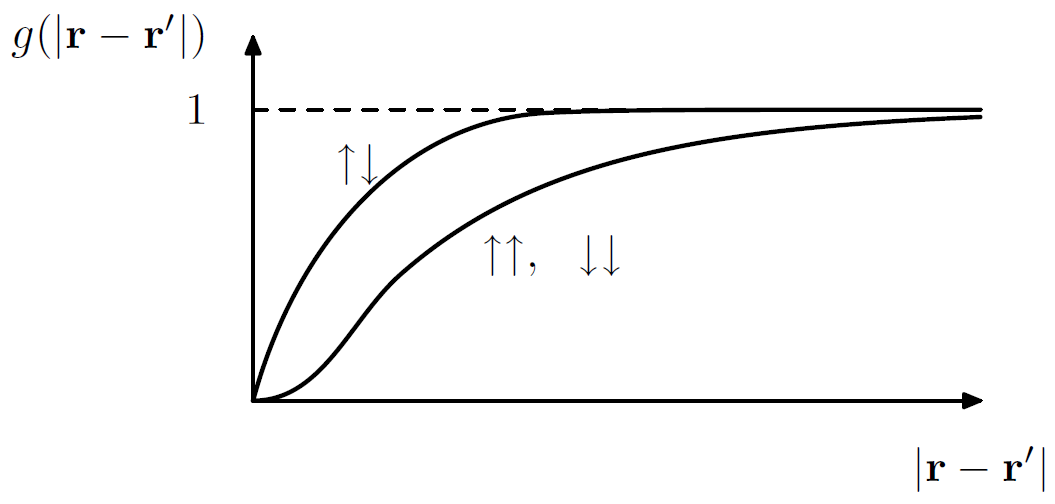
\includegraphics[width=0.7\textwidth]{immagini/funzione_di_correlazione.png}
\end{figure}
\hspace{-0.6cm}Questo effetto è detto \emph{exchange hole}, nel senso che descrive l'effetto dell'interazione di scambio che impedisce agli elettroni di occupare la stessa posizione. A questo si aggiunge la repulsione coulombiana, che introduce un costo energetico quando gli elettroni sono vicini: questo costituisce la parte di correlazione del problema exchange-correlation.\\
Il punto importante è comprendere il meccanismo complessivo, che deriva dall'azione combinata della repulsione coulombiana e del principio di esclusione. Il modo più semplice per descrivere questo effetto di schermaggio è utilizzare un potenziale coulombiano schermato, in cui lo screening è descritto dal modello di Thomas--Fermi come un decadimento esponenziale:
\begin{equation*}
   V_{\rm TF}
   = \frac{e^2}{4 \pi \varepsilon_0} \frac{1}{|\vb{r} - \vb{r'}|} e^{-|\vb{r} - \vb{r'}|/r_{\rm TF}}
\end{equation*}
Questo introduce di fatto una lunghezza caratteristica molto più corta per la repulsione coulombiana, che in linea di principio agirebbe a tutte le distanze.\\
\subsection{Interazione con i fononi}
Finora abbiamo considerato solo la parte elettronica, ma per comprendere la cosa accade nella transizione superconduttiva è necessario includere anche l'effetto delle vibrazioni del reticolo. L'indizio sperimentale che l'effetto da includere fosse proprio questo è l'effetto isotopico, cioè la dipendenza della temperatura critica dalla massa isotopica. Questo infatti suggerisce che il fenomeno coinvolge il moto dei nuclei attorno alle loro posizioni di equilibrio, cioè le vibrazioni del reticolo, ossia i fononi.\\
Il meccanismo può essere descritto tramite diagrammi di Feynman, che rappresentano un modo semplice per descrivere a livello grafico ciò che accade.
\begin{figure}[H]
   \centering
   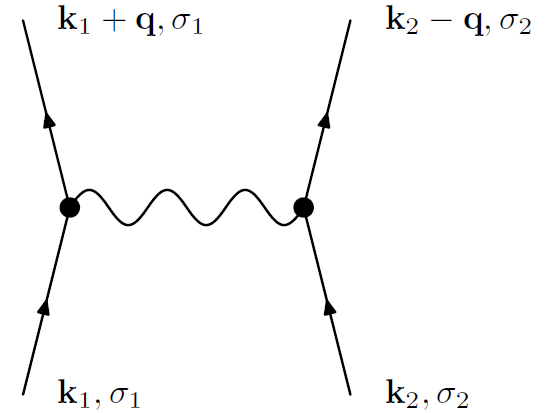
\includegraphics[width=0.45\textwidth]{immagini/diagramma_di_Feynman_1.png}
\end{figure}
\hspace{-0.6cm}Consideriamo un elettrone in uno stato di Bloch, caratterizzato quindi da due numeri quantici: $n$, legato alla sua energia, e $\vb{k}_2$, che è il suo momento. Inoltre esso possiede spin $\sigma_2$. In questa descrizione diagrammatica esso è rappresentato da una freccia.\\
Questo elettrone può emettere un fonone con quantità di moto $\hbar\vb{q}$, modificando quindi a causa di questa interazione, descritta da un punto nel diagramma, il proprio momento in $\vb{k}_2 - \vb{q}$. Il suo spin rimarrà invece invariato.\\
I fononi sono rappresentati da linee ondulate nel diagramma, per indicare la loro diversa natura e statistica. Il momento che acquisisce il fonone è $\hbar\vb{q}$, in modo che il momento totale sia conservato.\\
Un secondo elettrone, caratterizzato da $(\vb{k}_1,\sigma_1)$, può interagire con lo stesso fonone, acquisendo un momento maggiore $\vb{k}_1 + \vb{q}$, come se avesse assorbito il fonone, mantenendo lo stesso spin.\\
Questo processo rappresenta un'interazione efficace tra due elettroni, $(\vb{k}_1,\sigma_1)$ e $(\vb{k}_2,\sigma_2)$, mediata dallo scambio di un fonone.\mn{Questo meccanismo è generale: particelle fermioniche possono interagire tramite lo scambio di bosoni, come avviene anche nella fisica delle particelle.}\\
Ribadiamo il fatto che questa è una descrizione pittorica: non stiamo ancora spiegando perché un elettrone interagisca con un fonone. Per capire l'origine dell'interazione bisogna considerare il reticolo cristallino.\\
Consideriamo un cristallo con un atomo per cella unitaria. Possiamo studiare quali vibrazioni sono possibili nel reticolo. In particolare sappiamo che in questo caso possiamo avere un modo longitudinale e due modi trasversali.\\
Se vogliamo scrivere l'energia del reticolo includendo le vibrazioni, dobbiamo considerare che ogni vibrazione ha una certa frequenza $\omega$ e quindi un'energia $\hbar\omega$. Questa energia dipende dal momento, il quale è differente a seconda del tipo di modo.\\
Possiamo descrivere questi modi come oscillatori armonici e quindi la loro energia può essere scritta nella forma quantistica che conosciamo per l'oscillatore armonico. Se $a^{\dag}_{\vb{q},\lambda}$ e $a^{\vphantom{\dag}}_{\vb{q},\lambda}$ sono gli operatori di creazione e annichilazione di fononi con frequenza $\omega_{\vb{q},\lambda}$, allora l'energia dei modi del cristallo con un atomo per cella unitaria può essere espressa come una somma sui modi $\omega$ e sulle polarizzazioni $\lambda$:
\begin{equation*}
   H
   = \sum_{\vb{q},\lambda} \hbar \omega^{\vphantom{\dag}}_{\vb{q},\lambda} a_{\vb{q},\lambda}^{\dag} a^{\vphantom{\dag}}_{\vb{q},\lambda}
\end{equation*}
Questi modi, se interpretati nello spazio reale (mentre sono stati introdotti nello spazio dei momenti), corrispondono a spostamenti degli atomi rispetto alle loro posizioni di equilibrio. Indichiamo tali spostamenti con $\delta \vb{R}_i$, dove $\vb{R}_i$ è la posizione dell'$i$-esimo atomo del reticolo. Essi possono essere espressi in termini delle coordinate dei modi $(\vb{q},\lambda)$; in generale si ha una somma su tutti i modi, con il fattore tipico che compare quando si descrive la coordinata di un oscillatore armonico in termini degli operatori $a$ e $a^{\dag}$:
\begin{equation*}
   \delta \vb{R}_i
   =\sum_{\vb{q},\lambda} \vb{e}_{\vb{q},\lambda} \sqrt{\frac{\hbar}{2 M \omega_{\vb{q},\lambda}}} \qty( a^{\dag}_{\vb{q},\lambda} + a_{-\vb{q},\lambda} ) e^{i \vb{q} \vdot \vb{R}_i}
\end{equation*}
Un tale spostamento del reticolo cristallino produrrà una modulazione della densità di carica degli elettroni e del potenziale efficace per gli elettroni nel solido, $V_1(\vb{r})$. Possiamo definire il potenziale di deformazione come
\begin{equation*}
   \delta V_1(\vb{r})
   =\sum_i \delta \pdv{V_1(\vb{r})}{\vb{R}_i} \delta \vb{R}_i
\end{equation*}
Vediamo ora quali sono le conseguenze di questi spostamenti per gli elettroni che si muovono nel reticolo.
\begin{figure}[H]
   \centering
   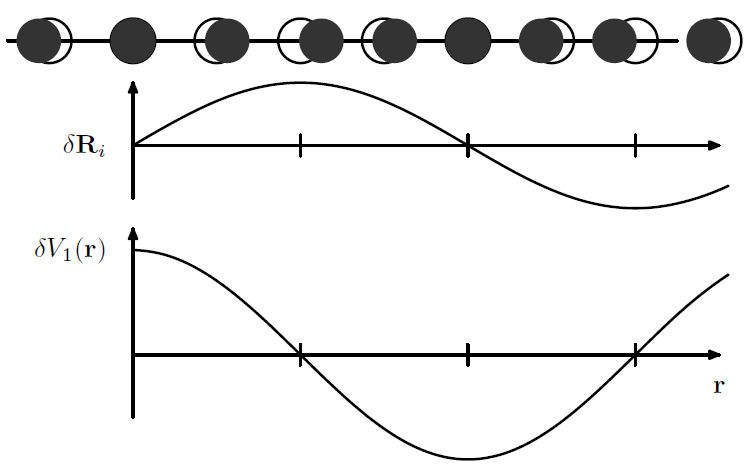
\includegraphics[width=0.7\textwidth]{immagini/reticolo_cristallino.png}
\end{figure}
\hspace{-0.6cm}La figura mostra schematicamente cosa accade quando gli atomi non si trovano più nelle loro posizioni di equilibrio, ma sono soggetti a uno spostamento $\delta \vb{R}_i$ associato a un modo di vibrazione del reticolo. Gli atomi risultano quindi leggermente dislocati: alcuni possono rimanere praticamente fermi, mentre altri si spostano in direzioni opposte in modo periodico lungo il reticolo.\\
Dal punto di vista fisico, questo è cruciale perché gli atomi in un metallo sono ioni, quindi portano carica positiva. Di conseguenza, una loro ridistribuzione nello spazio implica una modulazione della densità di carica positiva: si formano regioni in cui la densità è maggiore rispetto all'equilibrio e regioni in cui è minore.\\
Un elettrone che si muove nel reticolo “vede” quindi un potenziale elettrico che non è più uniforme: nelle regioni in cui la densità di carica positiva è maggiore, il potenziale è più attrattivo, mentre nelle regioni in cui è minore è meno attrattivo (o relativamente repulsivo rispetto alla configurazione uniforme).\\
Questo porta all'idea chiave: la vibrazione del reticolo genera una modulazione del potenziale che tende ad attirare gli elettroni verso le regioni di maggiore densità ionica. In tali regioni si crea una sorta di buca di potenziale in cui gli elettroni sono energeticamente favoriti a trovarsi.\\
Se consideriamo due elettroni liberi di muoversi nel reticolo, entrambi saranno attratti verso le stesse regioni di carica positiva aumentata. Questo può essere interpretato come un'interazione attrattiva efficace tra i due elettroni, anche se l'interazione fondamentale tra loro è repulsiva.\\
Questo è il meccanismo fisico alla base dell'interazione elettronica mediata dai fononi: la deformazione del reticolo (cioè i fononi) induce una deformazione del potenziale che favorisce l'avvicinamento degli elettroni. Questa è l'interpretazione fisica della descrizione diagrammatica introdotta tramite i diagrammi di Feynman.\\
In altre parole, la deformazione del reticolo corrisponde a una modulazione periodica con lunghezza d'onda $\frac{2\pi}{q}$, dove $q$ è il momento del fonone, e questo comporta una variazione del momento degli elettroni, analoga a un processo di scattering.
\begin{figure}[H]
   \centering
   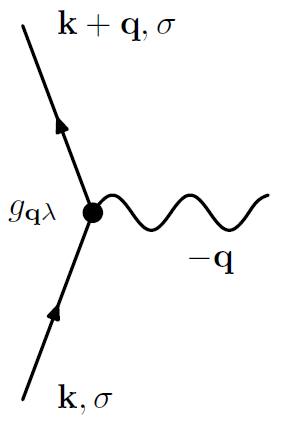
\includegraphics[width=0.25\textwidth]{immagini/diagramma_di_Feynman_2.png}
\end{figure}
\hspace{-0.6cm}Nel diagramma si rappresenta un elettrone che interagisce con il potenziale deformato. Diagrammaticamente questo corrisponde all'emissione o assorbimento di un fonone. Se un secondo elettrone interagisce con lo stesso fonone, il risultato complessivo è un'interazione efficace tra i due elettroni mediata dallo scambio del fonone.\\
Questa descrizione qualitativa può essere resa quantitativa introducendo un'interazione efficace tra elettroni che dipende dal momento del fonone e dalla frequenza:
\begin{equation}
   V_{\rm eff}(\vb{q},\omega)
   =|g_{\vb{q},\lambda}|^2 \frac{1}{\omega^2 - \omega_{\vb{q}}^2}
\end{equation}
Questa quantità risulta negativa quando $\omega < \omega_{\vb{q},\lambda}$, il che implica un'interazione attrattiva tra gli elettroni. Il coefficiente di accoppiamento segue la seguente dipendenza:
\begin{equation*}
   g_{\vb{q},\lambda}
   \propto \sqrt{\frac{m}{M}}
\end{equation*}
dove $m$ è la massa dell'elettrone e $M$ quella dell'isotopo. Questo fattore è tipicamente dell'ordine di $10^{-2}$, indicando che l'interazione è debole.\\
Prendiamo questa forma come punto di partenza. Bardeen, Cooper e Schrieffer introdussero una semplificazione importante: invece di considerare la dipendenza dal momento del fonone, si assume un'interazione efficace che dipende solo da una scala energetica caratteristica, la frequenza di Debye $\omega_D$, cioè la massima frequenza dei fononi:
\begin{equation*}
   V_{\rm eff}(\vb{q},\omega)
   =|g_{\rm eff}|^2 \frac{1}{\omega^2 - \omega_D^2}
\end{equation*}
Questo equivale a trascurare i dettagli microscopici dei singoli modi, mantenendo solo la scala energetica rilevante.\\
Poiché la superconduttività si manifesta a temperature $T < T_c$, la scala energetica associata è $k_B T_c$. Nei superconduttori convenzionali vale tipicamente $k_B T_c \ll \hbar \omega_D$, per cui si può trascurare la dipendenza dalla frequenza. L'interazione efficace diventa quindi:
\begin{equation*}
   V_{\rm eff}
   =-\frac{|g_{\rm eff}|^2}{\omega_D^2}
   \equiv - |V|^2
\end{equation*}
cioè una costante negativa.\\
A questo punto vogliamo scrivere l'hamiltoniana di interazione tra elettroni mediata dallo scambio di fononi. Nella teoria BCS si utilizzano operatori fermionici di creazione e annichilazione, $c^{\dag}$ e $c$, che rispettano le regole di anticommutazione per i fermioni. Poiché dipendono dal momento e dallo spin, li indichiamo con indici espliciti, cioè 
$c^{\dag}_{\vb{k},\sigma}$ e $c^{\vphantom{\dag}}_{\vb{k},\sigma}$, che sono rispettivamente l'operatore di creazione e annichilazione di un elettrone con momento $\vb{k}$ e spin $\sigma$.\\
Il processo descritto nel diagramma di Feynman è il seguente: due elettroni iniziali, $(\vb{k}_2,\sigma_2)$ e $(\vb{k}_1,\sigma_1)$, interagiscono scambiando un fonone, e dopo l'interazione diventano stati con momenti $\vb{k}_2 - \vb{q}$ e $\vb{k}_1 + \vb{q}$.\\
L'hamiltoniana deve quindi distruggere i due elettroni iniziali e creare i due finali:
\begin{equation}
   \hat{H}
   = - |V|^2 \sum_{\vb{k}} c^{\dag}_{\vb{k}_1 + \vb{q},\sigma_1} c^{\dag}_{\vb{k}_2 - \vb{q},\sigma_2} c^{\vphantom{\dag}}_{\vb{k}_1,\sigma_1} c^{\vphantom{\dag}}_{\vb{k}_2,\sigma_2}
   \label{eq:BCS_interaction_hamiltonian}
\end{equation}
Nel descrivere questo processo è fondamentale ricordare che, in un metallo, gli elettroni occupano gli stati fino all'energia di Fermi $E_F$. Di conseguenza, partecipano all'interazione solo gli elettroni vicini alla superficie di Fermi, cioè quelli per cui esistono stati disponibili in cui essere diffusi.
\begin{figure}[H]
   \centering
   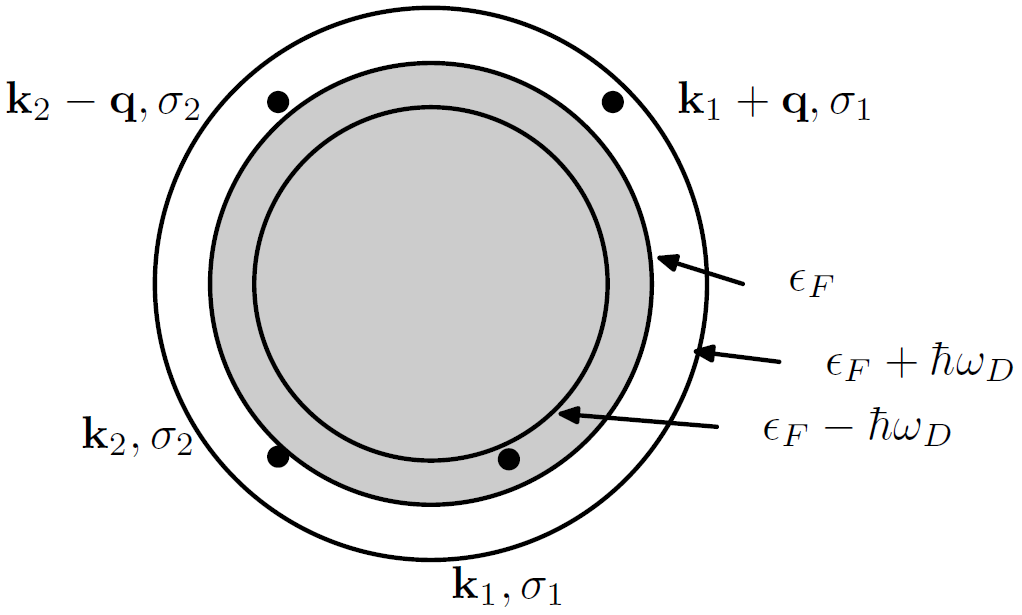
\includegraphics[width=0.5\textwidth]{immagini/superficie_di_Fermi.png}
\end{figure}
\hspace{-0.6cm}Gli elettroni coinvolti sono quindi confinati in una shell energetica attorno a $E_F$ di ampiezza dell'ordine di $\hbar \omega_D$: stati con energia inferiore a $E_F$ sono occupati, mentre quelli con energia maggiore sono disponibili.\\
Consideriamo quindi un elettrone con energia tra $E_F - \hbar \omega_D$ ed $E_F$, con momento $\vb{k}_1$. Dopo l'interazione con un fonone, esso può acquisire momento $\vb{k}_1 + \vb{q}$ ed essere diffuso in uno stato con energia superiore a $E_F$. Analogamente, un secondo elettrone vicino alla superficie di Fermi modifica il proprio stato.
\section{Problema di Cooper}
Vogliamo capire quale sia la struttura dello stato di due elettroni dopo che l'interazione attrattiva ha agito. In altre parole, vogliamo scrivere una funzione d'onda a due elettroni: questo è precisamente il cosiddetto \emph{problema di Cooper}. Esso consiste nello studiare lo stato di due elettroni che interagiscono tramite un'interazione attrattiva di qualche origine, e nel determinare quale relazione debba sussistere tra i loro momenti.\\
Supponiamo quindi di avere due elettroni con energia vicina al livello di Fermi. Quello che cerchiamo è la loro funzione d'onda, $\psi_0(\vb{r}_1,\vb{r}_2)$, a cui andrà poi aggiunta anche la parte di spin. Se i due elettroni hanno momenti $\vb{k}_1$ e $\vb{k}_2$, il loro momento totale è $\vb{K}=\vb{k}_1 + \vb{k}_2$.\\
Nel problema di Cooper, siamo interessati allo stato a energia minima di due elettroni sopra il mare di Fermi. Per argomenti generali,\sn{Il motivo per cui lo stato a energia minima ha momento totale nullo può essere compreso separando il moto dei due elettroni in moto del centro di massa e moto relativo. L'energia totale contiene infatti un contributo positivo associato al moto del centro di massa,
\begin{equation*}
   E=E_{\text{rel}} + \frac{\hbar^2 K^2}{4m}
\end{equation*}
dove $\vb{K}=\vb{k}_1 + \vb{k}_2$. Poiché il secondo termine è sempre positivo, l'energia è minima per $\vb{K}=0$, cioè quando i due elettroni hanno momenti opposti.} tale stato ha momento totale nullo, cioè
\begin{equation*}
   \vb{K}=\vb{k}_1 + \vb{k}_2=0
\end{equation*}
da cui segue che i due elettroni hanno momenti opposti:
\begin{equation*}
   \vb{k}_1=-\vb{k}_2\equiv \vb{k}
\end{equation*}
Di conseguenza, la parte spaziale della funzione d'onda può essere scritta come una sovrapposizione di stati con momenti opposti:
\begin{equation*}
   \psi_0(\vb{r}_1,\vb{r}_2)
   =\sum_{\vb{k}} g_{\vb{k}}\, e^{i \vb{k}\cdot \vb{r}_1} e^{-i \vb{k}\cdot \vb{r}_2}
\end{equation*}
Poiché gli elettroni sono fermioni, dobbiamo includere anche lo spin. Sappiamo che due spin $1/2$ possono combinarsi in uno stato di singoletto oppure in uno stato di tripletto. Nel primo caso la parte di spin è antisimmetrica, nel secondo è simmetrica.\\
Ricordiamo che lo stato totale di due fermioni deve essere complessivamente antisimmetrico rispetto allo scambio delle due particelle. Questo significa che possiamo avere una parte spaziale simmetrica moltiplicata per una parte di spin antisimmetrica, oppure una parte spaziale antisimmetrica moltiplicata per una parte di spin simmetrica.\\
Per capire la simmetria della parte spaziale, riscriviamo $\psi_0$ come
\begin{equation*}
   \begin{split}
      \psi_0(\vb{r}_1,\vb{r}_2)
      &=\sum_{\vb{k}} g_{\vb{k}}\, e^{i\vb{k}\cdot(\vb{r}_1-\vb{r}_2)}
      \\
      &=\sum_{\vb{k}} g_{\vb{k}}
      \Bigl\{
      \cos\bigl[\vb{k}\cdot(\vb{r}_1-\vb{r}_2)\bigr]
      + i \sin\bigl[\vb{k}\cdot(\vb{r}_1-\vb{r}_2)\bigr]
      \Bigr\}
   \end{split}
\end{equation*}
La parte con il coseno è simmetrica per scambio $\vb{r}_1 \leftrightarrow \vb{r}_2$, mentre quella con il seno è antisimmetrica. Quindi lo stato totale può essere o del tipo\mn{Nelle espressioni che seguono $\alpha_1$ indica lo stato di spin up della particella 1, mentre $\beta_1$ indica il suo stato di spin down, e analogamente per la particella 2.}
\begin{equation*}
   \psi_0(\vb{r}_1,\sigma_1;\vb{r}_2,\sigma_2)
   =\sum_{\vb{k}} g_{\vb{k}}
   \cos\bigl[\vb{k}\cdot(\vb{r}_1-\vb{r}_2)\bigr]
   \,(\alpha_1\beta_2-\beta_1\alpha_2)
\end{equation*}
oppure del tipo
\begin{equation*}
   \psi_0(\vb{r}_1,\sigma_1;\vb{r}_2,\sigma_2)
   =\sum_{\vb{k}} g_{\vb{k}}
   \sin\bigl[\vb{k}\cdot(\vb{r}_1-\vb{r}_2)\bigr]
   \times
   \begin{Bmatrix}
      \alpha_1\alpha_2\\[0.1cm]
      \frac{1}{\sqrt{2}}(\alpha_1\beta_2+\beta_1\alpha_2)\\[0.1cm]
      \beta_1\beta_2
   \end{Bmatrix}
\end{equation*}
Stiamo descrivendo un'interazione attrattiva tra due elettroni, quindi un'interazione che tende a portarli vicini tra loro. In questa situazione, lo stato favorito è il primo, cioè quello con parte spaziale simmetrica e parte di spin antisimmetrica. Infatti, se l'interazione è attrattiva, gli elettroni devono avere probabilità non nulla di trovarsi a piccola distanza relativa. La probabilità di trovare i due elettroni molto vicini è determinata dalla parte spaziale della funzione d'onda per $\vb{r}_1 \simeq \vb{r}_2$. In tal caso, la parte con il seno si annulla, mentre quella con il coseno resta diversa da zero. Di conseguenza, lo stato con singoletto di spin è quello energeticamente favorito. La funzione d'onda della coppia risulta quindi
\begin{equation}
   \psi_0
   =\sum_{\vb{k}} g_{\vb{k}}
   \cos\bigl[\vb{k}\cdot(\vb{r}_1-\vb{r}_2)\bigr]
   (\alpha_1\beta_2-\beta_1\alpha_2)
   \label{eq:cooper_pair_wavefunction}
\end{equation}
Questo è ciò che si chiama una \emph{coppia di Cooper}: una combinazione speciale di due elettroni con momenti opposti e spin opposti.\\
Una volta identificato questo stato, vogliamo verificare se esso abbia effettivamente energia più bassa rispetto a due elettroni non accoppiati. Per farlo, dobbiamo calcolare il valore medio dell'hamiltoniana totale nello stato $\ket*{\psi_0}$.\\
L'hamiltoniana totale è
\begin{equation*}
   \hat{H}
   =\hat{H}_0 + \hat{V}
\end{equation*}
dove $\hat{H}_0$ è l'hamiltoniana degli elettroni liberi:
\begin{equation}
   \hat{H}_0
   =\sum_{\vb{k},\sigma} \varepsilon_{\vb{k}} c^{\dag}_{\vb{k},\sigma} c^{\vphantom{\dag}}_{\vb{k},\sigma}
   \label{eq:free_electron_hamiltonian}
\end{equation}
con
\begin{equation*}
   \varepsilon_{\vb{k}}
   =\frac{\hbar^2 k^2}{2m}
\end{equation*}
mentre $\hat{V}$ rappresenta l'interazione attrattiva.\\
Cominciamo calcolando il valore medio di $\hat{H}_0$. Introduciamo la notazione di Dirac e indichiamo con $\ket*{\vb{k}}$ lo stato di coppia con momenti opposti $\vb{k}$ e $-\vb{k}$.\mn{Più precisamente, lo stato sarebbe qualcosa del tipo $\ket*{\vb{k},\uparrow;-\vb{k},\downarrow}$, e la sua parte spaziale è proporzionale a $\cos[\vb{k}\cdot(\vb{r}_1-\vb{r}_2)]$.} Poiché $\hat{H}_0$ non agisce sullo spin, nel calcolare tale valor medio possiamo concentrarci solo sulla parte orbitale. Si ha:
\begin{equation*}
   \begin{split}
      \expval*{\hat{H}_0}
      &=
      \Bigl(\sum_{\vb{k}'} g_{\vb{k}'}^* \bra*{\vb{k}'}\Bigr)
      \hat{H}_0
      \Bigl(\sum_{\vb{k}} g^{\vphantom{*}}_{\vb{k}} \ket*{\vb{k}}\Bigr)
      \\
      &=
      \sum_{\vb{k},\vb{k}'} g^*_{\vb{k}'} g^{\vphantom{*}}_{\vb{k}}
      \mel*{\vb{k}'}{\hat{H}_0}{\vb{k}}
   \end{split}
\end{equation*}
Esplicitiamo il termine $\mel*{\vb{k}'}{\hat{H}_0}{\vb{k}}$:
\begin{equation*}
   \mel*{\vb{k}'}{\hat{H}_0}{\vb{k}}
   =
   \sum_{\vb{k}'',\sigma} \varepsilon_{\vb{k}''}
   \mel*{\vb{k}'}{c^{\dag}_{\vb{k}'',\sigma} c^{\vphantom{\dag}}_{\vb{k}'',\sigma}}{\vb{k}}
\end{equation*}
L'operatore $c^{\dag}_{\vb{k}'',\sigma} c^{\vphantom{\dag}}_{\vb{k}'',\sigma}$ conta il numero di elettroni con momento $\vb{k}''$ e spin $\sigma$. Quando agisce su uno stato di coppia, dà contributo solo se quel momento e quello spin sono presenti nello stato, cioè
\begin{equation*}
   c^{\dag}_{\vb{k}'',\sigma} c^{\vphantom{\dag}}_{\vb{k}'',\sigma}
   \ket{\vb{k},\uparrow;\,-\vb{k},\downarrow}
   =
   \begin{cases}
      \ket{\vb{k},\uparrow;\,-\vb{k},\downarrow} 
      & \text{se } (\vb{k}'',\sigma)=(\vb{k},\uparrow)\ \text{o}\ (-\vb{k},\downarrow)\\[0.1cm]
      0 & \text{altrimenti}
   \end{cases}
\end{equation*}
Nel nostro caso lo stato contiene due elettroni, uno in $(\vb{k},\uparrow)$ e uno in $(-\vb{k},\downarrow)$, quindi l'energia libera totale della coppia è semplicemente
\begin{equation*}
   \varepsilon_{\vb{k}} + \varepsilon_{-\vb{k}}
   =2\varepsilon_{\vb{k}}
\end{equation*}
poiché $\varepsilon_{\vb{k}}=\varepsilon_{-\vb{k}}$. Ne segue che
\begin{equation*}
   \mel*{\vb{k}'}{\hat{H}_0}{\vb{k}}
   =2\varepsilon_{\vb{k}} \braket*{\vb{k}'}{\vb{k}}
   =2\varepsilon_{\vb{k}}\,\delta_{\vb{k}',\vb{k}}
\end{equation*}
Pertanto
\begin{equation*}
   \expval*{\hat{H}_0}
   =\sum_{\vb{k}} |g_{\vb{k}}|^2\, 2\varepsilon_{\vb{k}}
\end{equation*}
Passiamo ora al valore medio dell'interazione:
\begin{equation*}
   \expval*{\hat{V}}
   =\sum_{\vb{k},\vb{k}'} g_{\vb{k}'}^* g^{\vphantom{*}}_{\vb{k}}
   \mel*{\vb{k}'}{\hat{V}}{\vb{k}}
   =\sum_{\vb{k},\vb{k}'} g_{\vb{k}'}^* g^{\vphantom{*}}_{\vb{k}}\, V_{\vb{k}',\vb{k}}
\end{equation*}
dove $V_{\vb{k}',\vb{k}}=\mel*{\vb{k}'}{\hat{V}}{\vb{k}}$ è l'elemento di matrice dell'interazione tra due stati di coppia diversi.\\
Vogliamo determinare la condizione di equilibrio, cioè la condizione di minima energia. Consideriamo quindi
\begin{equation*}
   \expval{H_0 + V}
   =
   E \braket{\psi}{\psi}
\end{equation*}
Per quanto riguarda il secondo membro, abbiamo
\begin{equation*}
   \braket{\psi}{\psi}
   =
   \Bigl(\sum_{\vb{k}'} g_{\vb{k}'}^* \bra*{\vb{k}'}\Bigr)
   \Bigl(\sum_{\vb{k}} g^{\vphantom{*}}_{\vb{k}} \ket*{\vb{k}}\Bigr)
   =
   \sum_{\vb{k}} |g_{\vb{k}}|^2
\end{equation*}
Utilizzando i risultati precedenti otteniamo
\begin{equation*}
   \sum_{\vb{k}} |g_{\vb{k}}|^2 \, 2 \varepsilon_{\vb{k}}
   +
   \sum_{\vb{k},\vb{k}'} g_{\vb{k}'}^* g^{\vphantom{*}}_{\vb{k}} V^{\vphantom{*}}_{\vb{k}',\vb{k}}
   =
   E \sum_{\vb{k}} |g_{\vb{k}}|^2
\end{equation*}
Portando tutti i termini al primo membro:
\begin{equation*}
   \sum_{\vb{k}} |g_{\vb{k}}|^2 (2 \varepsilon_{\vb{k}} - E)
   +
   \sum_{\vb{k},\vb{k}'} g_{\vb{k}'}^* g^{\vphantom{*}}_{\vb{k}} V^{\vphantom{*}}_{\vb{k}',\vb{k}}
   = 0
\end{equation*}
Raccogliendo la somma su $\vb{k}$, possiamo scrivere
\begin{equation*}
   \sum_{\vb{k}}
   \Big\{
      |g_{\vb{k}}|^2 (2 \varepsilon_{\vb{k}} - E)
      +
      \sum_{\vb{k}'} g_{\vb{k}'}^* g^{\vphantom{*}}_{\vb{k}} \, V_{\vb{k}',\vb{k}}
   \Big\}
   = 0
\end{equation*}
Affinché questa relazione sia soddisfatta, imponiamo che il termine tra parentesi graffe si annulli per ogni $\vb{k}$:
\begin{equation*}
   |g_{\vb{k}}|^2 (2 \varepsilon_{\vb{k}} - E)
   +
   \sum_{\vb{k}'} g_{\vb{k}'}^* g^{\vphantom{*}}_{\vb{k}} \, V_{\vb{k}',\vb{k}}
   = 0
\end{equation*}
Mettendo in evidenza $g_{\vb{k}}$, otteniamo
\begin{equation*}
   g_{\vb{k}}
   \Big[
      g_{\vb{k}}^* (2 \varepsilon_{\vb{k}} - E)
      +
      \sum_{\vb{k}'} g_{\vb{k}'}^* V_{\vb{k}',\vb{k}}
   \Big]
   = 0
\end{equation*}
Scartando la soluzione banale $g_{\vb{k}} = 0$, si ha
\begin{equation*}
   g_{\vb{k}}^* (2 \varepsilon_{\vb{k}} - E)
   +
   \sum_{\vb{k}'} g_{\vb{k}'}^* V_{\vb{k}',\vb{k}}
   = 0
\end{equation*}
Prendendo il complesso coniugato:
\begin{equation*}
   g_{\vb{k}} (2 \varepsilon_{\vb{k}} - E)
   +
   \sum_{\vb{k}'} g_{\vb{k}'} V_{\vb{k}',\vb{k}}
   = 0
\end{equation*}
Da cui si può scrivere
\begin{equation*}
   g_{\vb{k}}
   =
   - \frac{\sum_{\vb{k}'} g_{\vb{k}'} V_{\vb{k}',\vb{k}}}{2 \varepsilon_{\vb{k}} - E}
\end{equation*}
In generale l'elemento di matrice $V_{\vb{k},\vb{k}'}$ dipende da $\vb{k}$ e $\vb{k}'$, perché deriva dall'interazione efficace mediata dai fononi\mn{\cite{Tinkham} $V_{\vb{k},\vb{k}'}$ descrive la forza dell'interazione per lo scattering di una coppia di elettroni con momenti $(\vb{k}',-\vb{k}')$ in una coppia con momenti $(\vb{k},-\vb{k})$.}. Tuttavia, Cooper fece l'assunzione semplificatrice che tale interazione sia costante all'interno della shell energetica rilevante:
\begin{equation*}
   V_{\vb{k},\vb{k}'}=V
   \qq{,}
   V<0
\end{equation*}
Questa è la cosiddetta \emph{assunzione di Cooper}. L'equazione precedente diventa allora
\begin{equation*}
   g_{\vb{k}}
   =-V\,\frac{\sum_{\vb{k}'} g_{\vb{k}'}}{2\varepsilon_{\vb{k}}-E}
\end{equation*}
Sommiamo ora su tutti i valori di $\vb{k}$:
\begin{equation*}
   \sum_{\vb{k}} g_{\vb{k}}
   =-V \sum_{\vb{k}} \frac{\sum_{\vb{k}'} g_{\vb{k}'}}{2\varepsilon_{\vb{k}}-E}
\end{equation*}
Poiché il fattore $\sum_{\vb{k}'} g_{\vb{k}'}$ è comune, si semplifica e si ottiene:
\begin{equation*}
   1
   =-V \sum_{\vb{k}} \frac{1}{2\varepsilon_{\vb{k}}-E}
\end{equation*}
Poiché la somma va estesa solo agli stati disponibili al di sopra del livello di Fermi, si ha
\begin{equation*}
   1
   =-V \sum_{k \ge k_F}
   \frac{1}{2\varepsilon_{\vb{k}}-E}
\end{equation*}
La sommatoria può essere sostituita con un integrale introducendo la densità degli stati. La shell energetica al di sopra del livello di Fermi che dobbiamo considerare è quella determinata dalla frequenza di Debye:
\begin{equation*}
   -\frac{1}{V}
   =\int_{E_F}^{E_F+\hbar\omega_D}
   \dd{\varepsilon}\,
   N(\varepsilon)\,
   \frac{1}{2\varepsilon-E}
\end{equation*}
Se la densità degli stati viene approssimata con il suo valore al livello di Fermi, $N(E_F)$, si ha
\begin{equation*}
   -\frac{1}{V}
   =N(E_F)\int_{E_F}^{E_F+\hbar\omega_D} \dd{\varepsilon} \frac{1}{2\varepsilon-E}
\end{equation*}
L'integrale dà
\begin{equation*}
   -\frac{1}{V}
   =\frac{N(E_F)}{2}
   \ln\qty[ \frac{2E_F+2\hbar\omega_D-E}{2E_F-E} ]
\end{equation*}
Esponenziando entrambi i membri:
\begin{equation*}
   e^{-2/[V N(E_F)]}
   =\frac{2E_F+2\hbar\omega_D-E}{2E_F-E}
   =1+\frac{2\hbar\omega_D}{2E_F-E}
\end{equation*}
Da cui, con qualche passaggio algebrico,
\begin{equation*}
   E
   =2E_F-\frac{2\hbar\omega_D}{e^{-2/[V N(E_F)]}-1}
\end{equation*}
Ponendo $V=-|V|$, cioè esplicitando che l'interazione è attrattiva, si ottiene
\begin{equation*}
   E
   =2E_F-\frac{2\hbar\omega_D}{e^{2/[|V|N(E_F)]}-1}
\end{equation*}
Poiché $|V|$ è piccolo,\mn{\cite{Tinkham} In gran parte dei superconduttori convenzionali si trova che $N(E_F) |V|<0.3$. Ciò permette di utilizzare la cosiddetta approssimazione di accoppiamento debole, valida per $N(E_F) |V| \ll 1$.} l'esponenziale è molto grande rispetto a $1$. Possiamo quindi fare l'approssimazione:
\begin{equation}
   E
   \simeq
   2E_F-2\hbar\omega_D\, e^{-2/[|V|N(E_F)]}
   \label{eq:energia_cooper}
\end{equation}
Questa espressione mostra che l'energia della coppia di Cooper è minore di $2E_F$, cioè minore dell'energia che avrebbero due elettroni indipendenti al livello di Fermi. Questo significa che, in presenza di un'interazione attrattiva, per quanto debole, i due elettroni preferiscono formare una coppia con momenti opposti e spin opposti.\\
Il punto fondamentale è che la correzione energetica non è una piccola correzione perturbativa proporzionale a $V$, ma ha una dipendenza esponenziale in $1/|V|$. Questo è un effetto essenzialmente non perturbativo, ed è uno degli aspetti più profondi del problema di Cooper.\sn{\cite{Tinkham} Si noti che che la forma dell'energia di legame non è analitica in $V=0$, cioè non può essere espansa in potenze di $V$. Di conseguenza, non può essere ottenuta tramite teoria perturbativa, un fatto che ha notevolmente ritardato la genesi della teoria.}.\\
Facciamo adesso alcuni commenti sulla struttura dello stato dato dall'\eqrefcustom{eq:cooper_pair_wavefunction}. I coefficienti $g_{\vb{k}}$ dipendono solo da $k^2$, e quindi non selezionano alcuna direzione privilegiata nello spazio. Questo corrisponde a un accoppiamento di tipo $s$, cioè a una simmetria sferica della coppia.\\
Un altro aspetto importante riguarda l'estensione spaziale della coppia. Essa può essere stimata a partire dal momento della coppia, che è legata alla velocità di Fermi $v_F$ in quanto gli elettroni coinvolti hanno energia vicina a $E_F$. D'altra parte, la scala energetica rilevante è data da $k_B T_c$, che è la scala energetica associata alla transizione superconduttiva. Si ottiene così una lunghezza caratteristica
\begin{equation*}
   \xi_0
   =\frac{\hbar v_F}{k_B T_c}
\end{equation*}
Questa quantità è dell'ordine della lunghezza di coerenza ed è tipicamente molto grande, dell'ordine di $10^4$\;\AA, se si usano valori tipici $v_F\sim 10^8\;\mathrm{cm/s}$ e $T_c\sim 10\;\mathrm{K}$.\\
Questo ci dice che la distanza media tra i due elettroni che formano una coppia di Cooper è molto maggiore della distanza interparticellare media. È importante sottolinearlo, perché si potrebbe essere portati a immaginare una coppia di Cooper come due elettroni molto vicini che si muovono insieme quasi come due palline legate. In realtà non è così: la coppia è un oggetto quantistico esteso. I due elettroni sono fortemente correlati, ma non sono necessariamente vicini nello spazio in senso classico.
\section{Stato fondamentale BCS}
A questo punto vogliamo capire quali siano le conseguenze delle proprietà dello stato di coppia di Cooper in un sistema reale, cioè in un solido. In altre parole, non consideriamo più una singola coppia di elettroni, ma un metallo in cui è presente un'interazione attrattiva tra molti elettroni. Questo ci porterà a determinare la struttura dello stato fondamentale nella teoria BCS.\\
Il punto cruciale è che abbiamo a che fare con uno stato a molti corpi di fermioni, quindi è necessario introdurre un certo formalismo matematico per determinarne la struttura.\\
Il punto di partenza è l'Hamiltoniana del sistema, che è composta da una parte di elettroni liberi e da una parte che descrive l'interazione, la quale assume la forma che abbiamo derivato considerando l'interazione mediata dai fononi.\\
Abbiamo assunto che l'interazione non dipenda da $\vb{k}$ e che sia negativa, a condizione che l'energia coinvolta sia minore dell'energia di Debye, che rappresenta la scala energetica rilevante.\\
Possiamo scrivere esplicitamente questa interazione utilizzando gli operatori fermionici di creazione e annichilazione che, come abbiamo visto, portano alla forma data nell'\eqrefcustom{eq:BCS_interaction_hamiltonian}, se consideriamo semplicemente i processi in cui due elettroni vengono diffusi tramite l'interazione con un fonone di momento generico.\\
Nel complesso, l'interazione comporta l'annichilazione di due elettroni e la creazione di altri due elettroni, ciascuno con momento diverso, ma in modo tale che il momento totale sia conservato. Inoltre, lo spin non è coinvolto nell'interazione, in quanto non viene modificato.
\subsection{Hamiltoniana di pairing}
Partiamo dallo scrivere quella che viene chiamata Hamiltoniana di pairing, cioè una Hamiltoniana che descrive questo meccanismo di interazione.\\
In essa abbiamo una parte di elettroni liberi, data da
\begin{equation*}
   H_0
   =\sum_{\vb{k},\sigma} \varepsilon(\vb{k}) c^{\dag}_{\vb{k},\sigma} c^{\vphantom{\dag}}_{\vb{k},\sigma}
\end{equation*}
e una parte di interazione data da\mn{Si presti attenzione al fatto che stiamo usando la notazione
\begin{equation*}
   -|V| \to \frac{V}{2}
\end{equation*}
}
\begin{equation*}
   H_I
   =\frac{V}{2} \sum_{\vb{k},\vb{k}',\vb{q}} \sum_{\sigma,\sigma'} 
   c^{\dag}_{\vb{k + q},\sigma} 
   c^{\dag}_{\vb{k' - q},\sigma'} 
   c^{\vphantom{\dag}}_{\vb{k}',\sigma'} 
   c^{\vphantom{\dag}}_{\vb{k},\sigma}
\end{equation*}
Poiché queste interazioni coinvolgono coppie di elettroni con combinazioni di momento e spin del tipo $(\vb{k},\uparrow)$ e $(-\vb{k},\downarrow)$, nella somma possiamo imporre che $\vb{k}'=-\vb{k}$ e $\sigma'=-\sigma$. In questo modo, nel termine di interazione non è più necessario sommare su $\vb{k}'$ e su $\sigma'$:
\begin{equation*}
   H_I
   =\frac{V}{2} \sum_{\vb{k},\vb{q}} \sum_{\sigma} 
   c^{\dag}_{\vb{k + q},\sigma} 
   c^{\dag}_{-\vb{k - q},-\sigma} 
   c^{\vphantom{\dag}}_{-\vb{k},-\sigma} 
   c^{\vphantom{\dag}}_{\vb{k},\sigma}
\end{equation*}
Se ora esplicitiamo le combinazioni di momento e spin che contribuiscono all'interazione, otteniamo\mn{Stiamo semplicemente introducendo il cambio di variabile $\vb{k}'=\vb{k}+\vb{q}$, di modo che il termine di interazione descriva lo scattering di una coppia $(\vb{k},-\vb{k})$ in una coppia $(\vb{k}',-\vb{k}')$.}
\begin{equation*}
   H_I
   = V \sum_{\vb{k},\vb{k}'} 
   c^{\dag}_{\vb{k'},\uparrow} 
   c^{\dag}_{-\vb{k'},\downarrow} 
   c^{\vphantom{\dag}}_{-\vb{k},\downarrow} 
   c^{\vphantom{\dag}}_{\vb{k},\uparrow}
\end{equation*}
Qui abbiamo introdotto un fattore 2, poiché $\sigma$ può assumere i valori $\uparrow$ o $\downarrow$ e, dato che l'interazione non dipende dallo spin, possiamo fissare un particolare ordine degli operatori (ad esempio $\uparrow, \downarrow, \downarrow, \uparrow$), tenendo conto che le altre combinazioni danno contributi equivalenti.\\
A questo punto introduciamo il cosiddetto operatore di creazione di una coppia di Cooper $Z^{\dag}_{\vb{k}}$, definito come
\begin{equation*}
   Z^{\dag}_{\vb{k}}
   =c^{\dag}_{\vb{k},\uparrow} c^{\dag}_{-\vb{k},\downarrow}
\end{equation*}
Si tratta quindi di un operatore composto da due operatori di creazione: uno per un elettrone $(\vb{k},\uparrow)$ e l'altro per un elettrone $(-\vb{k},\downarrow)$. Possiamo riscrivere il termine di interazione in funzione di questo operatore come
\begin{equation*}
   H_I
   = V \sum_{\vb{k}'} Z^{\dag}_{\vb{k}'} \sum_{\vb{k}} Z^{\vphantom{\dag}}_{\vb{k}}
   =\frac{1}{V} \hat{\Delta}^{\dag} \hat{\Delta}
\end{equation*}
dove abbiamo introdotto l'operatore
\begin{equation*}
   \hat{\Delta} \equiv V \sum_{\vb{k}} Z_{\vb{k}}
\end{equation*}
\subsection{Funzione d'onda di prova}
Ora dobbiamo capire, a partire da questo tipo di interazione, quale sia la struttura dello stato fondamentale. Il procedimento che utilizziamo è un procedimento variazionale: ciò significa che scriviamo una funzione d'onda di prova, introduciamo alcuni coefficienti e poi cerchiamo il minimo del valor medio dell'Hamiltoniana.\\
Per costruire la funzione d'onda di prova partiamo da ciò che già conosciamo, cioè il comportamento di un metallo in assenza di superconduttività. Infatti, dobbiamo partire da una funzione d'onda che, nel limite in cui l'interazione viene spenta, si riduca allo stato fondamentale degli elettroni liberi.\\
Lo stato fondamentale di un gas di Fermi non interagente, essendo costituito da elettroni liberi che occupano tutti gli stati con momento fino al momento di Fermi, può essere scritto come
\begin{equation*}
   \ket*{g_{\rm free}}
   =\prod_{k \leq k_F} Z^{\dag}_{\vb{k}} \ket*{0}
\end{equation*}
In questo modo consideriamo tutti gli stati con diversi valori di $k$ in forma di prodotto. Nulla vieta di raggruppare gli stati a due elettroni e scriverli come prodotto di coppie (dove con coppie non intendiamo ancora le coppie di Cooper, ma semplicemente coppie di elettroni).\\
Ricordiamo che l'operatore $Z^{\dag}_{\vb{k}}$ crea un elettrone $(\vb{k},\uparrow)$ e uno $(-\vb{k},\downarrow)$; quindi, se consideriamo per tutti i valori di $k<k_F$ uno stato del tipo
\begin{equation*}
   \prod_{k<k_F} \ket*{\vb{k},\uparrow} \hspace{-0.17cm} \ket*{-\vb{k},\downarrow}
\end{equation*}
otteniamo uno stato che descrive tutti gli elettroni liberi con momento minore di $k_F$.\\
Possiamo ora immaginare di costruire delle sovrapposizioni. In generale, sappiamo che in meccanica quantistica una particella può trovarsi in una sovrapposizione di stati. Se un sistema può essere negli stati $\ket*{a}$ e $\ket*{b}$, può anche trovarsi nello stato $c_a \ket*{a} + c_b \ket*{b}$, dove $\ket*{a}$ e $\ket*{b}$ sono autostati. Qui però vogliamo costruire una sovrapposizione di tipo particolare: ci chiediamo infatti se sia possibile costruire sovrapposizioni di stati con diverso numero di particelle, cioè stati del tipo
\begin{equation*}
   \ket*{\psi}=u \ket*{0_{\vb{k}}} + \nu \ket*{2_{\vb{k}}}
\end{equation*}
Questo stato rappresenta una sovrapposizione di uno stato con zero particelle di momento $\vb{k}$ e uno stato con due particelle. Precisiamo che lo stato $\ket*{2_{\vb{k}}}$ è definito come
\begin{equation*}
   \ket*{2_{\vb{k}}}
   =Z^{\dag}_{\vb{k}} \ket*{0_{\vb{k}}}
\end{equation*}
cioè come l'azione dell'operatore di creazione di coppia con momento $\vb{k}$ sullo stato vuoto. Si tratta quindi di uno stato con due elettroni aventi momenti opposti e spin opposti. In altre parole, il simbolo “2” indica il numero di elettroni, mentre $\vb{k}$ identifica il valore del momento associato alla coppia.\\
Lo stato che abbiamo scritto è una sovrapposizione quantistica di due stati, ma con una differenza rispetto ai casi usuali: si tratta infatti di una sovrapposizione di stati con numero diverso di particelle. Vedremo che la struttura dello stato fondamentale BCS è proprio di questo tipo:
\begin{equation}
   \ket*{g_s}
   =\prod_{\vb{k}} \bigl( u_{\vb{k}} \ket*{0_{\vb{k}}} + \nu_{\vb{k}} \ket{2_{\vb{k}}} \bigr)
   \label{eq:BCS_trial_wavefunction}
\end{equation}
Questo stato è quindi il prodotto, su tutti i valori di $\vb{k}$,\mn{Con “tutti i valori di $\vb{k}$” si intendono sia quelli minori che maggiori di $k_F$.} di sovrapposizioni di stati con zero e due particelle. In altre parole, la funzione d'onda di prova che utilizzeremo per minimizzare il valor medio dell'Hamiltoniana è costruita come prodotto, su tutti i $\vb{k}$, di sovrapposizioni di stati con zero e due elettroni, dove i due elettroni sono quelli creati dall'operatore di coppia.\\
Consideriamo una sovrapposizione di questi due stati perché, come abbiamo visto, l'interazione attrattiva ha la forma di un termine che distrugge tutte le possibili coppie moltiplicato per un termine che crea tutte le possibili coppie, cioè $\hat{\Delta}^{\dag}\hat{\Delta}$. Dalla struttura dell'interazione nasce quindi l'idea di cercare stati di questo tipo.\\
Un punto importante da osservare è che uno stato di questa forma non ha un numero fissato di particelle, poiché in generale contiene contributi con diverso numero di elettroni.\\
A questo punto dobbiamo calcolare il valor medio dell'Hamiltoniana, includendo il termine di interazione. Il primo passo consiste nello scrivere esplicitamente questo valor medio sullo stato di prova, mentre il secondo passo consiste nel minimizzarlo rispetto ai coefficienti, che sono proprio $u_{\vb{k}}$ e $\nu_{\vb{k}}$.\\
Prima di procedere, facciamo un'osservazione: in assenza di interazione non devono comparire stati $\ket*{2_{\vb{k}}}$ per $k > k_F$, quindi i coefficienti $\nu_{\vb{k}}$ devono essere legati alla presenza dell'interazione. Vogliamo allora che, nel limite in cui $V \to 0$, lo stato di prova $\ket*{g_s}$ si riduca allo stato fondamentale degli elettroni liberi $\ket*{g_{\rm free}}$.\\
Ciò richiede che, per $V \to 0$,
\begin{equation*}
   u_{\vb{k}}
   =
   \begin{cases}
      0 & \text{per }k<k_F\\
      1 & \text{per }k>k_F
   \end{cases}
   \qq{,}
   \nu_{\vb{k}}
   =
   \begin{cases}
      1 & \text{per }k<k_F\\
      0 & \text{per }k>k_F
   \end{cases}
\end{equation*}
In questo modo, per $k<k_F$ le coppie risultano occupate, mentre per $k>k_F$ risultano vuote, riproducendo il mare di Fermi degli elettroni liberi.\\
Un'ulteriore condizione da imporre è la normalizzazione degli stati, che richiede
\begin{equation}
   |u_{\vb{k}}|^2 + |\nu_{\vb{k}}|^2
   =1
   \label{eq:BCS_normalization_condition}
\end{equation}
\subsection{Box di Nambu}
Lo stato dato dall'\eqrefcustom{eq:BCS_trial_wavefunction} è uno stato prodotto che coinvolge, per ogni $\vb{k}$, una sovrapposizione degli stati $\ket*{0_{\vb{k}}}$ e $\ket*{2_{\vb{k}}}$. Questo significa che la funzione d'onda di prova è fattorizzata rispetto ai diversi valori di $\vb{k}$: ogni coppia $(\vb{k}, -\vb{k})$ è descritta da una sovrapposizione indipendente, senza correlazioni dirette tra sottospazi con momenti diversi.\\
Torniamo ora ai due elettroni che formano queste sovrapposizioni: uno è nello stato $(\vb{k},\uparrow)$ e l'altro in $(-\vb{k},\downarrow)$. Considerando questi due stati, si possono avere diverse configurazioni possibili: nessun elettrone, entrambi gli elettroni, oppure un solo elettrone in uno dei due stati e nessuno nell'altro. In altre parole, lo spazio degli stati accessibili è costituito da quattro configurazioni:
\begin{equation*}
   \begin{array}{ll}
      \ket*{0}=\ket*{0_{\vb{k},\uparrow}; 0_{-\vb{k},\downarrow}} 
      & \ket*{2}=\ket*{1_{\vb{k},\uparrow}; 1_{-\vb{k},\downarrow}}\\[0.2cm]
      \ket*{+}=\ket*{1_{\vb{k},\uparrow}; 0_{-\vb{k},\downarrow}} 
      & \ket*{-}=\ket*{0_{\vb{k},\uparrow}; 1_{-\vb{k},\downarrow}}
   \end{array}
\end{equation*}
Questo sottospazio dello spazio di Hilbert totale, associato a un dato $\vb{k}$, prende il nome di \textit{box di Nambu}. Un box di Nambu consiste quindi nel considerare due livelli elettronici, $(\vb{k},\uparrow)$ e $(-\vb{k},\downarrow)$, e tutte le possibili occupazioni: zero, uno o due elettroni. Lo stato $\ket*{0}$ corrisponde all'assenza di elettroni in entrambi i livelli, lo stato $\ket*{2}$ alla presenza di entrambi gli elettroni, mentre $\ket*{+}$ e $\ket*{-}$ rappresentano gli stati con un solo elettrone. Si tratta quindi di uno spazio di Fock a quattro dimensioni. Vedremo che lavorare in termini di box di Nambu è particolarmente conveniente per trattare la funzione d'onda di prova.\\
Consideriamo ora l'azione dell'operatore di creazione di coppia in questo box.
\begin{figure}[H]
   \centering
   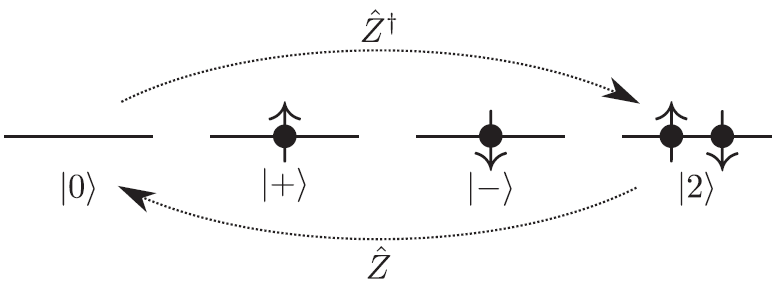
\includegraphics[width=0.6\textwidth]{immagini/azione_Zk_Nambu_box.png}
\end{figure}
\hspace{-0.6cm}Esso trasforma $\ket*{0_{\vb{k}}}$ in $\ket*{2_{\vb{k}}}$, mentre non connette direttamente gli stati $\ket*{+}$ e $\ket*{-}$, poiché è composto da due operatori di creazione. Di conseguenza, per quanto riguarda l'interazione, possiamo limitarci al sottospazio bidimensionale generato da $\ket*{0_{\vb{k}}}$ e $\ket*{2_{\vb{k}}}$. Gli altri due stati non vengono considerati in questa fase, ma è importante ricordare che possono diventare rilevanti quando si studiano le eccitazioni rispetto allo stato fondamentale.\\
In questo sottospazio possiamo utilizzare la notazione dei sistemi a due livelli. In particolare si ha\mn{Si noti che la base è stata scelta in modo che $\ket*{2_{\vb{k}}}$ sia il primo vettore di base e $\ket*{0_{\vb{k}}}$ il secondo.}
\begin{equation*}
   \ket*{0_{\vb{k}}}
   =\begin{pmatrix}
      0\\
      1
   \end{pmatrix}
   \qq{;}
   \ket*{2_{\vb{k}}}
   =\begin{pmatrix}
      1\\
      0
   \end{pmatrix}
\end{equation*}
L'operatore di creazione di coppia assume quindi la forma matriciale
\begin{equation*}
   Z^{\dag}_{\vb{k}}
   =\begin{pmatrix}
      0 & 1 \\
      0 & 0
   \end{pmatrix}
\end{equation*}
infatti
\begin{equation*}
   Z^{\dag}_{\vb{k}} \ket*{0_{\vb{k}}}
   =
   \begin{pmatrix}
      0 & 1 \\
      0 & 0
   \end{pmatrix}
   \begin{pmatrix}
      0\\
      1
   \end{pmatrix}
   =
   \begin{pmatrix}
      1\\
      0
   \end{pmatrix}
   =\ket*{2_{\vb{k}}}
\end{equation*}
Analogamente, l'operatore di annichilazione di coppia è dato da
\begin{equation*}
   Z_{\vb{k}}
   =\begin{pmatrix}
      0 & 0 \\
      1 & 0
   \end{pmatrix}
\end{equation*}
Con questa descrizione, lo spazio di Fock a molti corpi può essere visto come prodotto diretto di tutti i box di Nambu, e la funzione d'onda di prova per lo stato fondamentale può essere riscritta come
\begin{equation}
   \ket*{g_s}
   =\prod_{\vb{k}} \bigl( u_{\vb{k}} + \nu_{\vb{k}} Z^{\dag}_{\vb{k}} \bigr) \ket*{0}
   \label{eq:BCS_trial_wavefunction_Nambu}
\end{equation}
dove ora $\ket*{0}$ rappresenta lo stato di vuoto globale, cioè lo stato senza elettroni per qualunque valore di $\vb{k}$ e dello spin.
\subsection{Energia dello stato fondamentale}
Passiamo ora al calcolo dell'energia dello stato fondamentale a partire dalla funzione d'onda di prova. Precisiamo che, poiché stiamo considerando uno stato in cui il numero di particelle non è fissato (essendo una sovrapposizione), nel metodo variazionale dobbiamo introdurre un moltiplicatore di Lagrange. In questo caso, tale vincolo è legato al numero medio di particelle, che entra attraverso il potenziale chimico.\\
Ciò significa che, partendo dall'Hamiltoniana totale, dobbiamo includere un termine che tenga conto del fatto che il numero di particelle non è fissato. Questo si realizza aggiungendo il termine $-\mu \hat{N}$, dove l'operatore numero è
\begin{equation*}
   \hat{N}
   =\sum_{\vb{k},\sigma} c^{\dag}_{\vb{k},\sigma} c^{\vphantom{\dag}}_{\vb{k},\sigma}
\end{equation*}
L'Hamiltoniana effettiva da utilizzare nel metodo variazionale diventa quindi
\begin{equation*}
   \hat{H}=\hat{H}_0 - \mu \hat{N} + \hat{H}_I
\end{equation*}
L'effetto di questo termine sulle energie è semplice, poiché ha la stessa struttura di $\hat{H}_0$ vista nell'\eqrefcustom{eq:free_electron_hamiltonian}. In pratica, introduce uno shift delle energie pari al potenziale chimico. Definendo
\begin{equation*}
   \xi_{\vb{k}}
   =\varepsilon(\vb{k}) - \mu
\end{equation*}
che rappresenta l'energia rispetto al livello di Fermi, possiamo riscrivere
\begin{equation*}
   \hat{H}_0 - \mu \hat{N}
   =\sum_{\vb{k},\sigma} \xi(\vb{k}) c^{\dag}_{\vb{k},\sigma} c^{\vphantom{\dag}}_{\vb{k},\sigma}
   =\sum_{\vb{k},\sigma} \xi(\vb{k}) \hat{n}_{\vb{k},\sigma}
\end{equation*}
dove $\hat{n}_{\vb{k},\sigma}=c^{\dag}_{\vb{k},\sigma} c^{\vphantom{\dag}}_{\vb{k},\sigma}$ è l'operatore numero.\\
Il primo passo consiste nel calcolare il numero medio di particelle sullo stato di prova, cioè $\expval*{\hat{N}}$; il secondo passo è valutare $\expval*{(\hat{N} - \expval*{\hat{N}})^2}$; senza entrare nei dettagli del calcolo, si trova che la deviazione quadratica media
\begin{equation*}
   \delta N_{\rm rms}
   =\sqrt{\big\langle \bigl( \hat{N} - \expval*{\hat{N}} \bigr)^2 \big\rangle}
\end{equation*}
scala come la radice quadrata del numero medio di particelle. Di conseguenza,
\begin{equation*}
   \frac{\delta N_{\rm rms}}{\expval*{\hat{N}}}
   \propto \frac{\sqrt{N}}{N}
   =\frac{1}{\sqrt{N}}
\end{equation*}
Poiché $N$ è il numero medio di elettroni nel sistema ed è quindi macroscopicamente grande, questa quantità è molto piccola. Questo significa che, pur considerando uno stato in cui il numero di particelle non è fissato, le fluttuazioni relative del numero di particelle sono trascurabili. Di conseguenza, lo stato BCS può essere considerato, a tutti gli effetti pratici, equivalente a uno stato con numero di particelle fissato, in quanto l'errore relativo è trascurabile nel limite macroscopico.\mn{\cite{Tinkham} Nel formalismo BCS lo stato fondamentale non ha un numero fissato di particelle, tuttavia, poiché il numero di elettroni in un metallo è macroscopicamente grande, le fluttuazioni relative del numero di particelle sono trascurabili. Di conseguenza, non si introduce alcun errore significativo lavorando con uno stato in cui è fissato soltanto il numero medio di particelle.\\
Inoltre, ciò corrisponde a lavorare in un ensemble grand-canonico, che è più conveniente dal punto di vista matematico.}
\\
Passiamo ora al calcolo di $\expval*{\hat{H}_0 - \mu \hat{N}}$:
\begin{equation*}
   \expval*{\hat{H}_0 - \mu \hat{N}}
   =\mel{g_s}{\sum_{\vb{k},\sigma} \xi(\vb{k}) \hat{n}_{\vb{k},\sigma}}{g_s}
   =\mel{g_s}{\sum_{\vb{k}} \xi(\vb{k}) \bigl[ \hat{n}_{\vb{k},\uparrow} + \hat{n}_{-\vb{k},\downarrow} \bigr]}{g_s}
\end{equation*}
dove nell'ultimo passaggio abbiamo esplicitato la somma sugli spin.\\
Scriviamo ora lo stato come prodotto sui box di Nambu:
\begin{equation*}
   \ket*{g_s}
   =\prod_{\vb{k}} \ket*{g_{\vb{k}}}
\end{equation*}
Si ottiene quindi
\begin{equation*}
   \begin{split}
      \expval*{\hat{H}_0 - \mu \hat{N}}
      & =\prod_{\vb{k}'} \bra*{g_{\vb{k}'}}
      \sum_{\vb{k}} \xi(\vb{k}) \bigl[ \hat{n}_{\vb{k},\uparrow} + \hat{n}_{-\vb{k},\downarrow} \bigr]
      \prod_{\vb{k}''} \ket*{g_{\vb{k}''}}
      \\
      & =\sum_{\vb{k}} \xi(\vb{k}) \prod_{\vb{k}'} \bra*{g_{\vb{k}'}}
      \bigl[ \hat{n}_{\vb{k},\uparrow} + \hat{n}_{-\vb{k},\downarrow} \bigr]
      \prod_{\vb{k}''} \ket*{g_{\vb{k}''}}
   \end{split}
\end{equation*}
Osserviamo i seguenti fatti:
\begin{itemize}[leftmargin=0.5cm]
   \item Poiché la funzione di prova è fattorizzata rispetto ai diversi valori di $\vb{k}$, quando calcoliamo il prodotto scalare dello stato totale otteniamo un prodotto di prodotti scalari, ciascuno associato a un particolare valore di $\vb{k}$. Ad esempio, se consideriamo un sistema con due valori di $\vb{k}$, $\vb{k}_1$ e $\vb{k}_2$, avremo
   \begin{equation*}
      \ket*{g_s} = \ket*{g_{\vb{k}_1}} \otimes \ket*{g_{\vb{k}_2}}
   \end{equation*}
   e quindi
   \begin{equation*}
      \braket*{g_s}{g_s}
      = \braket*{g_{\vb{k}_1}}{g_{\vb{k}_1}} \cdot \braket*{g_{\vb{k}_2}}{g_{\vb{k}_2}}
   \end{equation*}
   \item L'operatore numero agisce in maniera non banale solo nel box di Nambu associato a $\vb{k}$, mentre sui box con $\vb{k}$ diverso si comporta come l'identità. Se consideriamo di nuovo il caso con due valori di $\vb{k}$ e prendiamo, ad esempio, l'operatore numero associato a $\vb{k}_1$, il suo valor medio sarà
   \begin{equation*}
      \begin{split}
         \mel*{g_s}{\hat{n}_{\vb{k}_1,\uparrow} + \hat{n}_{-\vb{k}_1,\downarrow}}{g_s}
         & =
         \mel*{g_{\vb{k}_1}}{\hat{n}_{\vb{k}_1,\uparrow} + \hat{n}_{-\vb{k}_1,\downarrow}}{g_{\vb{k}_1}}
         \cdot \braket*{g_{\vb{k}_2}}{g_{\vb{k}_2}}
         \\[0.1cm]
         & =
         \mel*{g_{\vb{k}_1}}{\hat{n}_{\vb{k}_1,\uparrow} + \hat{n}_{-\vb{k}_1,\downarrow}}{g_{\vb{k}_1}}
      \end{split}
   \end{equation*}
   in quanto $\braket*{g_{\vb{k}_2}}{g_{\vb{k}_2}}=1$ per la normalizzazione.
\end{itemize}
In generale, per ogni termine della somma, l'operatore numero agisce in maniera non banale solo nel box di Nambu associato a quel particolare $\vb{k}$, mentre su tutti gli altri box si comporta come l'identità. Di conseguenza, nel calcolo del valor medio possiamo limitarci al box di Nambu associato a quel particolare $\vb{k}$, poiché sugli altri box si ottiene semplicemente un fattore unitario. Pertanto
\begin{equation*}
   \expval*{\hat{H}_0 - \mu \hat{N}}
   =\sum_{\vb{k}} \xi(\vb{k}) \mel*{g_{\vb{k}}}{\bigl[ \hat{n}_{\vb{k},\uparrow} + \hat{n}_{-\vb{k},\downarrow} \bigr]}{g_{\vb{k}}}
\end{equation*}
A questo punto, per svolgere più agevolmente il calcolo, adoperiamo la notazione matriciale.\\
Consideriamo il termine generico della somma. Ricordiamo che
\begin{equation*}
   \ket*{g_{\vb{k}}}
   =u_{\vb{k}} \ket*{0_{\vb{k}}} + \nu_{\vb{k}} \ket*{2_{\vb{k}}}
   =
   \begin{pmatrix}
      \nu_{\vb{k}}\\
      u_{\vb{k}}
   \end{pmatrix}
\end{equation*}
L'operatore $\hat{n}_{\vb{k},\uparrow} + \hat{n}_{-\vb{k},\downarrow}$ conta il numero di elettroni nei due stati $(\vb{k},\uparrow)$ e $(-\vb{k},\downarrow)$. Nella base $\{\ket*{2_{\vb{k}}}, \ket*{0_{\vb{k}}}\}$\, esso è rappresentato da
\begin{equation*}
   \hat{n}_{\vb{k},\uparrow} + \hat{n}_{-\vb{k},\downarrow}
   =\begin{pmatrix}
      2 & 0 \\
      0 & 0
   \end{pmatrix}
\end{equation*}
Infatti, applicato a $\ket*{0_{\vb{k}}}$ dà 0, mentre applicato a $\ket*{2_{\vb{k}}}$ dà 2.\\
Il valor medio risulta quindi
\begin{equation*}
   \begin{split}
      \mel*{g_{\vb{k}}}
      {\bigl[ \hat{n}_{\vb{k},\uparrow} + \hat{n}_{-\vb{k},\downarrow} \bigr]}
      {g_{\vb{k}}}
      & =
      \begin{pmatrix}
         \nu^*_{\vb{k}} & u^*_{\vb{k}}
      \end{pmatrix}
      \begin{pmatrix}
         2 & 0 \\
         0 & 0
      \end{pmatrix}
      \begin{pmatrix}
         \nu_{\vb{k}} \\
         u_{\vb{k}}
      \end{pmatrix}
      = 2 |\nu_{\vb{k}}|^2
   \end{split}
\end{equation*}
dove $|\nu_{\vb{k}}|^2$ rappresenta la probabilità che la coppia con momento $\vb{k}$ sia occupata.\\
In conclusione, abbiamo ottenuto che
\begin{equation*}
   \mel*{g_s}{\hat{H}_0 - \mu \hat{N}}{g_s}
   =2\sum_{\vb{k}} \xi(\vb{k}) |\nu_{\vb{k}}|^2
\end{equation*}
Il passo successivo consiste nel calcolare il valor medio del termine di interazione. Questo termine è più complesso, perché contiene gli operatori complessivi di creazione e annichilazione. Per valutarlo utilizziamo la cosiddetta \textit{approssimazione di campo medio} (\textit{mean field approximation}), che in questo caso consiste nel sostituire il valor medio del prodotto di due operatori con il prodotto dei rispettivi valori medi:
\begin{equation*}
   \expval*{\hat{H}_I}
   =\frac{1}{V} \expval*{\hat{\Delta}^{\dag} \hat{\Delta}}
   \approx \frac{1}{V} \expval*{\hat{\Delta}^{\dag}} \hspace{-0.17cm} \expval*{\hat{\Delta}}
\end{equation*}
L'idea dell'approssimazione di campo medio è la seguente: se abbiamo un sistema costituito da molte particelle tutte interagenti tra loro, e non siamo interessati ai dettagli della singola interazione tra ciascuna particella e tutte le altre, ma piuttosto allo stato collettivo del sistema, allora possiamo assumere che ogni particella interagisca con il campo medio generato da tutte le altre. Questa approssimazione può fornire una descrizione ragionevole del sistema quando il numero di particelle è molto grande.\\
Nel nostro caso, poiché il numero di particelle è grande e vogliamo valutare il valor medio dell'operatore $\hat{\Delta}^{\dag}\hat{\Delta}$, che in linea di principio coinvolge tutte le coppie, il calcolo esatto richiederebbe di tenere conto di tutte queste interazioni. Se però assumiamo che ciascuna coppia interagisca con il campo medio prodotto da tutte le altre, allora possiamo fattorizzare il valor medio del prodotto nel prodotto dei valori medi, trascurando un contributo piccolo. Questa approssimazione è giustificata nello stesso senso in cui è giustificato considerare uno stato a numero non fissato di particelle: l'errore relativo è piccolo quando il numero di particelle è macroscopico.\\
In queste condizioni il problema si semplifica, perché dobbiamo calcolare valori medi più semplici. Consideriamo ad esempio $\expval*{\hat{\Delta}}$. Si ha
\begin{equation*}
   \expval*{\hat{\Delta}}
   =V \mel*{g_s}{\sum_{\vb{k}} Z_{\vb{k}}}{g_s}
   =V \sum_{\vb{k}} \mel*{g_{\vb{k}}}{Z_{\vb{k}}}{g_{\vb{k}}}
\end{equation*}
dove abbiamo implicitamente utilizzato il fatto che l'operatore $Z_{\vb{k}}$ agisce solo nel box di Nambu con momento $\vb{k}$; di conseguenza, il valor medio si riduce alla somma dei contributi dei singoli box di Nambu.\\
Usando nuovamente la rappresentazione matriciale, otteniamo
\begin{equation*}
   \mel*{g_{\vb{k}}}{Z_{\vb{k}}}{g_{\vb{k}}}
   =
   \begin{pmatrix}
      \nu^*_{\vb{k}} & u^*_{\vb{k}}
   \end{pmatrix}
   \begin{pmatrix}
      0 & 0 \\
      1 & 0
   \end{pmatrix}
   \begin{pmatrix}
      \nu_{\vb{k}} \\
      u_{\vb{k}}
   \end{pmatrix}
   =
   \begin{pmatrix}
      \nu^*_{\vb{k}} & u^*_{\vb{k}}
   \end{pmatrix}
   \begin{pmatrix}
      0\\
      \nu_{\vb{k}}
   \end{pmatrix}
   =u^*_{\vb{k}} \nu_{\vb{k}}
\end{equation*}
Quindi
\begin{equation*}
   \expval*{\hat{\Delta}}
   =V \sum_{\vb{k}} u^*_{\vb{k}} \nu_{\vb{k}}
\end{equation*}
L'altro valor medio è semplicemente il complesso coniugato:
\begin{equation*}
   \expval*{\hat{\Delta}^{\dag}}
   =V \sum_{\vb{k}} \nu^*_{\vb{k}} u_{\vb{k}}
\end{equation*}
Mettendo insieme i due risultati, si ottiene
\begin{equation*}
   \frac{1}{V} \expval*{\hat{\Delta}^{\dag} \hat{\Delta}}
   \simeq \frac{V^2}{V} \Bigl( \sum_{\vb{k}} \nu^*_{\vb{k}} u_{\vb{k}} \Bigr) \Bigl( \sum_{\vb{k}} u^*_{\vb{k}} \nu_{\vb{k}} \Bigr)
   = V \Bigl| \sum_{\vb{k}} u_{\vb{k}} \nu^*_{\vb{k}} \Bigr|^2
\end{equation*}
In definitiva, il valor medio dell'Hamiltoniana sullo stato di prova, in approssimazione di campo medio, risulta
\begin{equation}
   \begin{split}
      E
      =\expval*{\hat{H}}
      & =\mel*{g_s}{\hat{H}_0 - \mu \hat{N} + \hat{H}_I}{g_s}
      \\
      & =\sum_{\vb{k}} 2 \xi(\vb{k}) |\nu_{\vb{k}}|^2
      + V \Bigl| \sum_{\vb{k}} u_{\vb{k}} \nu^*_{\vb{k}} \Bigr|^2
   \end{split}
   \label{eq:BCS_energy}
\end{equation}
Questa è l'espressione generale dell'energia che ora dobbiamo minimizzare, poiché il nostro obiettivo è determinare in modo variazionale l'energia dello stato fondamentale. Si tratta quindi di un problema di minimizzazione in cui le quantità incognite sono $u_{\vb{k}}$ e $\nu_{\vb{k}}$ per tutti i valori di $\vb{k}$.\\
Prima di svolgere esplicitamente il calcolo, possiamo verificare cosa accade in assenza di interazione. Se $V=0$, l'energia si riduce a
\begin{equation*}
   E
   =\sum_{\vb{k}} 2 \xi(\vb{k}) |\nu_{\vb{k}}|^2
\end{equation*}
dove $\vb{k}$ può essere tale che $|\vb{k}|<k_F$ oppure $|\vb{k}|>k_F$. Vediamo cosa accade in questi due casi. Ricordiamo che
\begin{equation*}
   \xi(\vb{k})=\varepsilon(\vb{k}) - \mu
\end{equation*}
e che a temperatura nulla il potenziale chimico coincide con l'energia di Fermi, quindi possiamo porre $\mu=E_F$. Allora:
\begin{itemize}[leftmargin=0.5cm]
   \item se $k < k_F$, si ha $\varepsilon(\vb{k})<E_F$, e quindi $\xi(\vb{k})<0$;
   \item se $k > k_F$, si ha $\varepsilon(\vb{k})>E_F$, e quindi $\xi(\vb{k})>0$.
\end{itemize}
A questo punto ci chiediamo quali siano i valori di $\nu_{\vb{k}}$ che minimizzano l'energia.
\begin{itemize}[leftmargin=0.5cm]
   \item Per $k < k_F$, poiché $\xi(\vb{k})$ è negativa, l'energia è minima quando $|\nu_{\vb{k}}|^2 \to 1$, perché in questo modo il termine $\xi(\vb{k}) |\nu_{\vb{k}}|^2$ assume il valore più piccolo possibile.
   \item Per $k > k_F$, poiché $\xi(\vb{k})$ è positiva, l'energia è minima quando $|\nu_{\vb{k}}|^2 \to 0$, perché in questo modo il termine $\xi(\vb{k}) |\nu_{\vb{k}}|^2$ si annulla.
\end{itemize}
Nel complesso, questo significa che l'energia minima variazionale, nel caso in cui si spenga l'interazione, è
\begin{equation*}
   E_{\rm min}
   =\sum_{k < k_F} 2 \bigl[ \varepsilon(\vb{k}) - E_F \bigr]
\end{equation*}
Se guardiamo ora allo stato corrispondente, riconosciamo che esso coincide con lo stato fondamentale del mare di Fermi non interagente.\\
Quello che vediamo quindi è che, almeno fino a questo punto, la costruzione è sensata: se spegniamo l'interazione e minimizziamo l'energia, ritroviamo sia l'energia degli elettroni liberi sia i coefficienti corretti. Infatti, per $k < k_F$ si ha $\nu_{\vb{k}} \to 1$, per cui lo stato è $\ket*{g_{\vb{k}}}=\ket*{2_{\vb{k}}}$, mentre per $k > k_F$ si ha $\nu_{\vb{k}} \to 0$, per cui lo stato è $\ket*{g_{\vb{k}}}=\ket*{0_{\vb{k}}}$.
\subsection{Minimizzazione dell'energia}
Passiamo ora alla determinazione dello stato fondamentale variazionale nel caso generale in cui l'interazione sia presente. Quello che dobbiamo fare è minimizzare $E$ rispetto a $u_{\vb{k}}$ e $\nu_{\vb{k}}$, con il vincolo di normalizzazione in ciascun box di Nambu dato dall'\eqrefcustom{eq:BCS_normalization_condition}. Inoltre, bisogna tenere presente che in generale $u_{\vb{k}}$ e $u_{\vb{k}}^*$ sono due variabili indipendenti; quindi, quello che faremo sarà considerare la minimizzazione rispetto a ciascuna coppia di variabili $u_{\vb{k}}$ e $\nu_{\vb{k}}$, trattando i complessi coniugati come fissati.\\
Una volta scritta l'energia in funzione di $u_{\vb{k}}$ e $\nu_{\vb{k}}$, considereremo la variazione di $E$ rispetto a $u_{\vb{k}}$ e $\nu_{\vb{k}}$, mantenendo fissi $u_{\vb{k}}^*$ e $\nu_{\vb{k}}^*$. Imporremo poi la condizione $\delta E=0$ e, poiché vedremo che essa avrà la forma
\begin{equation*}
   \delta E
   =(\ldots)\,\delta u_{\vb{k}} + (\ldots)\,\delta \nu_{\vb{k}}
\end{equation*}
dalla condizione $\delta E=0$ otterremo due equazioni, imponendo che si annullino indipendentemente i coefficienti di $\delta u_{\vb{k}}$ e $\delta \nu_{\vb{k}}$. In questo modo ricaveremo due equazioni per ogni valore di $\vb{k}$, che ci permetteranno di determinare $u_{\vb{k}}$ e $\nu_{\vb{k}}$.\\
Quello che dobbiamo fare adesso è quindi manipolare l'espressione di $E$ in modo da scrivere esplicitamente $\delta E$ in funzione di $\delta u_{\vb{k}}$ e $\delta \nu_{\vb{k}}$.\\
Partiamo dal termine cinetico. Si ha
\begin{equation*}
   \delta \Bigl( \sum_{\vb{k}} 2 \xi(\vb{k}) |\nu_{\vb{k}}|^2 \Bigr)
   =\sum_{\vb{k}} 2 \xi(\vb{k}) \, \delta \bigl( |\nu_{\vb{k}}|^2 \bigr)
\end{equation*}
Ma poiché $|\nu_{\vb{k}}|^2=\nu^{\vphantom{*}}_{\vb{k}}\nu_{\vb{k}}^*$ e stiamo considerando $\nu_{\vb{k}}^*$ come fissato, si ha
\begin{equation*}
   \delta \bigl( |\nu_{\vb{k}}|^2 \bigr)
   =\nu_{\vb{k}}^*\, \delta \nu_{\vb{k}}
\end{equation*}
Quindi possiamo scrivere
\begin{equation*}
   \delta \Bigl( \sum_{\vb{k}} 2 \xi(\vb{k}) |\nu_{\vb{k}}|^2 \Bigr)
   =\sum_{\vb{k}} 2 \xi(\vb{k}) \nu_{\vb{k}}^* \,\delta \nu^{\vphantom{*}}_{\vb{k}}
\end{equation*}
Consideriamo ora il termine di interazione. Dobbiamo scrivere esplicitamente il modulo quadro della somma:
\begin{equation*}
   V \Bigl| \sum_{\vb{k}} u_{\vb{k}} \nu_{\vb{k}}^* \Bigr|^2
   =V \sum_{\vb{k}} u_{\vb{k}} \nu_{\vb{k}}^* \sum_{\vb{k}} u_{\vb{k}}^* \nu_{\vb{k}}
\end{equation*}
Ricordiamo che la seconda somma proviene dal valor medio di $\hat{\Delta}$, quindi possiamo indicarla con $\Delta$, mentre la prima proviene dal valor medio di $\hat{\Delta}^\dagger$, e possiamo quindi indicarla con $\Delta^*$. Possiamo allora scrivere
\begin{equation*}
   V \Bigl| \sum_{\vb{k}} u_{\vb{k}} \nu_{\vb{k}}^* \Bigr|^2
   =\sum_{\vb{k}} u_{\vb{k}} \nu_{\vb{k}}^* \,\Delta
   =\Delta^* \sum_{\vb{k}} u_{\vb{k}}^* \nu_{\vb{k}}
\end{equation*}
Di conseguenza, quando dobbiamo valutare la variazione del modulo quadro di questa somma, otteniamo
\begin{equation*}
   \begin{split}
      \delta \Bigl( V \Bigl| \sum_{\vb{k}} u_{\vb{k}} \nu_{\vb{k}}^* \Bigr|^2 \Bigr)
      & =\delta \Bigl( V \sum_{\vb{k}} u_{\vb{k}} \nu_{\vb{k}}^* \sum_{\vb{k}} u_{\vb{k}}^* \nu_{\vb{k}} \Bigr)
      \\
      & =\delta \Bigl( \sum_{\vb{k}} u_{\vb{k}} \nu_{\vb{k}}^* \Bigr)\, V \sum_{\vb{k}} u_{\vb{k}}^* \nu_{\vb{k}}
      +
      V \sum_{\vb{k}} u_{\vb{k}} \nu_{\vb{k}}^* \,\delta \Bigl( \sum_{\vb{k}} u_{\vb{k}}^* \nu_{\vb{k}} \Bigr)
      \\
      & =\sum_{\vb{k}} \delta u_{\vb{k}}\, \nu_{\vb{k}}^* \,\Delta
      +
      \Delta^* \sum_{\vb{k}} u_{\vb{k}}^* \,\delta \nu_{\vb{k}}
   \end{split}
\end{equation*}
cioè
\begin{equation*}
   \delta \Bigl( V \Bigl| \sum_{\vb{k}} u_{\vb{k}} \nu_{\vb{k}}^* \Bigr|^2 \Bigr)
   = \sum_{\vb{k}} \bigl[ \delta u_{\vb{k}} \,\nu_{\vb{k}}^* \,\Delta + \Delta^* u_{\vb{k}}^* \,\delta \nu_{\vb{k}} \bigr]
\end{equation*}
In definitiva, la variazione totale dell'energia è data da
\begin{equation}
   \delta E
   =\sum_{\vb{k}}
   2\xi(\vb{k}) \nu_{\vb{k}}^* \delta \nu_{\vb{k}}
   + \Delta \nu_{\vb{k}}^* \delta u_{\vb{k}}
   + \Delta^* u_{\vb{k}}^* \delta \nu_{\vb{k}}
   \label{eq:variation_energy}
\end{equation}
L'\eqrefcustom{eq:variation_energy} rappresenta, per ogni $\vb{k}$, una relazione nelle variabili $u_{\vb{k}}$ e $\nu_{\vb{k}}$. A prima vista sembrerebbe difficile trovare una soluzione, ma bisogna ricordare che abbiamo anche la condizione di normalizzazione data dall'\eqrefcustom{eq:BCS_normalization_condition}, che implica
\begin{equation*}
   \delta \bigl( |u_{\vb{k}}|^2 + |\nu_{\vb{k}}|^2 \bigr)
   =0
\end{equation*}
Poiché stiamo trattando $u_{\vb{k}}^*$ e $\nu_{\vb{k}}^*$ come fissati, questa condizione può essere riscritta come
\begin{equation*}
   u_{\vb{k}}^* \delta u_{\vb{k}}
   +
   \nu_{\vb{k}}^* \delta \nu_{\vb{k}}
   =0
\end{equation*}
Questa è una seconda relazione, che lega $\delta u_{\vb{k}}$ e $\delta \nu_{\vb{k}}$ per ogni valore di $\vb{k}$. Essa ci consente di esprimere una variazione in funzione dell'altra:
\begin{equation}
   \delta \nu_{\vb{k}}
   =-\frac{u_{\vb{k}}^*}{\nu_{\vb{k}}^*} \delta u_{\vb{k}}
   \label{eq:variation_normalization}
\end{equation}
Sostituendo l'\eqrefcustom{eq:variation_normalization} nell' \eqrefcustom{eq:variation_energy}, otteniamo un'equazione contenente solo $\delta u_{\vb{k}}$:
\begin{equation*}
   \begin{split}
      \delta E
      & =\sum_{\vb{k}}
      2\xi(\vb{k}) \nu_{\vb{k}}^*
      \Bigl( -\frac{u_{\vb{k}}^*}{\nu_{\vb{k}}^*} \delta u_{\vb{k}} \Bigr)
      + \Delta \nu_{\vb{k}}^* \delta u_{\vb{k}}
      + \Delta^* u_{\vb{k}}^*
      \Bigl( -\frac{u_{\vb{k}}^*}{\nu_{\vb{k}}^*} \delta u_{\vb{k}} \Bigr)
      \\
      & =\sum_{\vb{k}}
      \qty[
      -2\xi(\vb{k}) u_{\vb{k}}^*
      + \Delta \nu_{\vb{k}}^*
      - \Delta^* \frac{{(u_{\vb{k}}^*)}^2}{\nu_{\vb{k}}^*}
      ]
      \delta u_{\vb{k}}
   \end{split}
\end{equation*}
Poiché vogliamo trovare il minimo, imponiamo che questa variazione sia nulla. Questo porta alla condizione che, per ogni valore di $\vb{k}$, debbano annullarsi sia il coefficiente di $\delta u_{\vb{k}}$ che il suo complesso coniugato\sn{Questo è dovuto al fatto che, in principio, dovremmo valutare $\delta E$ considerando $u_{\vb{k}}$, $u_{\vb{k}}^*$, $\nu_{\vb{k}}$ e $\nu_{\vb{k}}^*$ come variabili indipendenti. Per semplificare il calcolo, si effettua dapprima la variazione rispetto a $u_{\vb{k}}$ e $\nu_{\vb{k}}$, mantenendo fissi i rispettivi complessi coniugati. Successivamente si dovrebbero fissare $u_{\vb{k}}$ e $\nu_{\vb{k}}$ e calcolare la variazione rispetto a $u_{\vb{k}}^*$ e $\nu_{\vb{k}}^*$. Tuttavia, poiché l'energia è una quantità reale, l'equazione ottenuta in questo secondo passaggio si ricava più semplicemente prendendo il complesso coniugato della precedente.}:
\begin{equation*}
   \begin{dcases}
      -2\xi(\vb{k}) u_{\vb{k}}^*
      + \Delta \nu_{\vb{k}}^*
      - \Delta^* \dfrac{{(u_{\vb{k}}^*)}^2}{\nu_{\vb{k}}^*}
      =0
      \\[0.2cm]
      -2\xi(\vb{k}) u_{\vb{k}}
      + \Delta^* \nu_{\vb{k}}
      - \Delta \dfrac{u_{\vb{k}}^2}{\nu_{\vb{k}}}
      =0
   \end{dcases}
\end{equation*}
Vogliamo ora semplificare queste equazioni, utilizzando le altre informazioni a nostra disposizione. In particolare, useremo la condizione di normalizzazione per eliminare $\Delta^*$. Per fare ciò, moltiplichiamo la prima equazione per $\nu_{\vb{k}}$ e la seconda per ${(u_{\vb{k}}^*)}^2/\nu_{\vb{k}}^*$:
\begin{equation*}
   \begin{dcases}
      -2\xi(\vb{k}) u_{\vb{k}}^* \nu^{\hphantom{*}}_{\vb{k}}
      + \Delta \nu_{\vb{k}}^* \nu^{\hphantom{*}}_{\vb{k}}
      - \Delta^* \dfrac{(u_{\vb{k}}^*)^2}{\nu_{\vb{k}}^*} \nu^{\hphantom{*}}_{\vb{k}}
      =0
      \\[0.2cm]
      -2\xi(\vb{k}) u_{\vb{k}} \dfrac{(u_{\vb{k}}^*)^2}{\nu_{\vb{k}}^*}
      + \Delta^* \nu_{\vb{k}} \dfrac{(u_{\vb{k}}^*)^2}{\nu_{\vb{k}}^*}
      - \Delta \dfrac{u_{\vb{k}}^2}{\nu_{\vb{k}}}\dfrac{(u_{\vb{k}}^*)^2}{\nu_{\vb{k}}^*}
      =0
   \end{dcases}
\end{equation*}
Sommando le due equazioni si elimina $\Delta^*$:
\begin{equation*}
   -2\xi(\vb{k}) \qty[ u_{\vb{k}}^* \nu_{\vb{k}}
   + u_{\vb{k}} \frac{(u_{\vb{k}}^*)^2}{\nu_{\vb{k}}^*} ]
   + \Delta \qty[ \nu_{\vb{k}}^* \nu_{\vb{k}}
   - \frac{u_{\vb{k}}^2}{\nu_{\vb{k}}} \frac{(u_{\vb{k}}^*)^2}{\nu_{\vb{k}}^*} ]
   =0
\end{equation*}
Tale espressione può essere riscritta come
\begin{equation*}
   -2\xi(\vb{k}) \frac{u_{\vb{k}}^*}{\nu_{\vb{k}}^*}\qty( |\nu_{\vb{k}}|^2 + |u_{\vb{k}}|^2 )
   + \Delta \qty( |\nu_{\vb{k}}|^2 - \frac{|u_{\vb{k}}|^4}{|\nu_{\vb{k}}|^2} )
   =0
\end{equation*}
Osserviamo che si ha
\begin{equation*}
   \begin{split}
      |\nu_{\vb{k}}|^2 - \frac{|u_{\vb{k}}|^4}{|\nu_{\vb{k}}|^2}
      & =\frac{1}{|\nu_{\vb{k}}|^2} \qty( |\nu_{\vb{k}}|^4 - |u_{\vb{k}}|^4 )
      \\
      & =\frac{1}{|\nu_{\vb{k}}|^2} \qty( |\nu_{\vb{k}}|^2 - |u_{\vb{k}}|^2 ) \qty( |\nu_{\vb{k}}|^2 + |u_{\vb{k}}|^2 )
      \\
      & =\frac{1}{|\nu_{\vb{k}}|^2} \qty( |\nu_{\vb{k}}|^2 - |u_{\vb{k}}|^2 )
   \end{split}
\end{equation*}
dove nell'ultimo passaggio abbiamo usato l'\eqrefcustom{eq:BCS_normalization_condition}. Tornando quindi all'equazione precedente, si ottiene
\begin{equation*}
   -2\xi(\vb{k}) \frac{u_{\vb{k}}^*}{\nu_{\vb{k}}^*}
   + \frac{\Delta}{|\nu_{\vb{k}}|^2} \qty( |\nu_{\vb{k}}|^2 - |u_{\vb{k}}|^2 )
   =0
\end{equation*}
Se moltiplichiamo entrambi i membri per $|\nu_{\vb{k}}|^2$ e riordiniamo i termini, otteniamo
\begin{equation}
   2\xi(\vb{k}) u_{\vb{k}}^* \nu_{\vb{k}}
   = \Delta \qty( |\nu_{\vb{k}}|^2 - |u_{\vb{k}}|^2 )
   \label{eq:BCS_intermediate_equation}
\end{equation}
Ora prendiamo il modulo quadro di questa equazione. Il motivo è che al secondo membro compaiono già moduli quadrati, mentre al primo no; in questo modo otteniamo una relazione contenente solo quantità reali e positive:
\begin{equation*}
   4 \xi^2(\vb{k}) |u_{\vb{k}}|^2 |\nu_{\vb{k}}|^2
   = |\Delta|^2 \qty( |\nu_{\vb{k}}|^2 - |u_{\vb{k}}|^2 )^2
\end{equation*}
Manipoliamo ancora questa equazione usando la condizione di normalizzazione. Sviluppando il quadrato al secondo membro si ha
\begin{equation*}
   \begin{split}
      \qty( |\nu_{\vb{k}}|^2 - |u_{\vb{k}}|^2 )^2
      & = |\nu_{\vb{k}}|^4 + |u_{\vb{k}}|^4 - 2 |u_{\vb{k}}|^2 |\nu_{\vb{k}}|^2
      \\
      & = \qty( |\nu_{\vb{k}}|^2 + |u_{\vb{k}}|^2 )^2 - 4 |u_{\vb{k}}|^2 |\nu_{\vb{k}}|^2
      \\
      & = 1 - 4 |u_{\vb{k}}|^2 |\nu_{\vb{k}}|^2
   \end{split}
\end{equation*}
dove abbiamo aggiunto e sottratto un termine 2 $|u_{\vb{k}}|^2 |\nu_{\vb{k}}|^2$ nel secondo passaggio in modo da ottenere il quadrato della somma, e nell'ultimo passaggio abbiamo usato la normalizzazione.\\
Sostituendo questo risultato nell'equazione precedente, si ottiene
\begin{equation*}
   4 \xi^2(\vb{k}) |u_{\vb{k}}|^2 |\nu_{\vb{k}}|^2
   = |\Delta|^2 \qty( 1 - 4 |u_{\vb{k}}|^2 |\nu_{\vb{k}}|^2 )
\end{equation*}
Da questa relazione possiamo isolare direttamente il prodotto $4|u_{\vb{k}}|^2|\nu_{\vb{k}}|^2$:
\begin{equation*}
   4 |u_{\vb{k}}|^2 |\nu_{\vb{k}}|^2
   =\frac{|\Delta|^2}{\xi^2(\vb{k}) + |\Delta|^2}
\end{equation*}
Dall'\eqrefcustom{eq:BCS_normalization_condition} si ricava che $|\nu_{\vb{k}}|^2 = 1 - |u_{\vb{k}}|^2$. Sostituendo questa relazione nell'equazione precedente, otteniamo
\begin{equation*}
   4 |u_{\vb{k}}|^2 (1 - |u_{\vb{k}}|^2)
   =\frac{|\Delta|^2}{\xi^2(\vb{k}) + |\Delta|^2}
\end{equation*}
ossia
\begin{equation*}
   -4 |u_{\vb{k}}|^4
   +4 |u_{\vb{k}}|^2
   -\frac{|\Delta|^2}{\xi^2(\vb{k}) + |\Delta|^2}
   =0
\end{equation*}
Questa è un'equazione algebrica di secondo grado nella variabile $|u_{\vb{k}}|^2$, che può essere risolta con la formula standard. Si ottiene
\begin{equation*}
   |u_{\vb{k}}|^2
   =\frac{1}{2} \qty( 1 \pm \sqrt{1 - \frac{|\Delta|^2}{\xi^2(\vb{k}) + |\Delta|^2}} )
\end{equation*}
Semplificando la radice quadrata, la si può riscrivere come
\begin{equation*}
   |u_{\vb{k}}|^2
   =\frac{1}{2} \qty( 1 \pm \frac{\xi(\vb{k})}{\sqrt{\xi^2(\vb{k}) + |\Delta|^2}} )
\end{equation*}
Una volta noto $|u_{\vb{k}}|^2$, dalla normalizzazione si ottiene immediatamente anche $|\nu_{\vb{k}}|^2$:
\begin{equation*}
   |\nu_{\vb{k}}|^2
   =\frac{1}{2} \qty( 1 \mp \frac{\xi(\vb{k})}{\sqrt{\xi^2(\vb{k}) + |\Delta|^2}} )
\end{equation*}
In questo modo otteniamo una forma esplicita per i due coefficienti che compaiono nello stato fondamentale BCS. Resta però da stabilire quale sia il segno corretto. Per farlo utilizziamo ciò che già sappiamo: nel limite in cui l'interazione si annulla, ciascuno stato $\ket*{g_{\vb{k}}}$ deve ridursi alla componente con momento $\vb{k}$ dello stato fondamentale del gas di Fermi normale, costituito da tutti gli elettroni con $k < k_F$.\\
Consideriamo quindi il limite $\Delta \to 0$. In tale limite resta solo $\xi(\vb{k})$ sia al numeratore che al denominatore, e il suo segno dipende dal fatto che $\varepsilon_{\vb{k}}$ sia minore o maggiore dell'energia di Fermi. Se $\varepsilon_{\vb{k}}>E_F$, lo stato deve essere vuoto, perché stiamo tornando allo stato fondamentale del gas di Fermi normale, in cui gli stati sopra il livello di Fermi non sono occupati. Nella nostra notazione, questo significa che il coefficiente $\nu_{\vb{k}}$ deve andare a zero, essendo il coefficiente associato allo stato con due elettroni. Viceversa, se $\varepsilon_{\vb{k}}<E_F$, cioè per livelli sotto l'energia di Fermi, gli elettroni devono essere presenti, e quindi $\nu_{\vb{k}}$ deve tendere a 1. Questo porta a scegliere il segno $+$ per $u_{\vb{k}}$ e il segno $-$ per $\nu_{\vb{k}}$.\\
Verifichiamolo esplicitamente. Nel limite $\Delta \to 0$ si ha
\begin{equation*}
   \lim_{\Delta \to 0} |\nu_{\vb{k}}|^2
   =\frac{1}{2} \qty( 1 - \frac{\xi(\vb{k})}{|\xi(\vb{k})|} )
   =\begin{cases}
      0 & \text{se } \xi(\vb{k})>0
      \\[0.1cm]
      1 & \text{se } \xi(\vb{k})<0
   \end{cases}
\end{equation*}
Possiamo quindi scrivere le espressioni finali dei due coefficienti:
\begin{align}
   |u_{\vb{k}}|^2
   &= \frac{1}{2} \qty(1 + \frac{\xi(\vb{k})}{\sqrt{\xi^2(\vb{k}) + |\Delta|^2}})
   \label{eq:coefficiente_u_BCS}
   \\[0.2cm]
   |\nu_{\vb{k}}|^2
   &= \frac{1}{2} \qty(1 - \frac{\xi(\vb{k})}{\sqrt{\xi^2(\vb{k}) + |\Delta|^2}})
   \label{eq:coefficiente_nu_BCS}
\end{align}
\subsection{Condizione di autoconsistenza}
Emerge però un ulteriore vincolo: il parametro $\Delta$ dipende esso stesso dai coefficienti $u_{\vb{k}}$ e $\nu_{\vb{k}}$. Pertanto, le soluzioni ottenute per tali coefficienti devono essere compatibili con la definizione di $\Delta$. Sostituendo $u_{\vb{k}}$ e $\nu_{\vb{k}}$ nella definizione del parametro d'ordine si ottiene infatti un'equazione di autoconsistenza, che determina i valori ammissibili di $\Delta$.\\
Torniamo quindi all'\eqrefcustom{eq:BCS_intermediate_equation}. Sostituendo i risultati ottenuti si ha
\begin{equation*}
   -2 \xi(\vb{k}) u^*_{\vb{k}} \nu_{\vb{k}}
   =\Delta \frac{ \xi(\vb{k}) }{ \sqrt{ \xi^2(\vb{k}) + |\Delta|^2 } }
\end{equation*}
Semplificando $\xi(\vb{k})$ da entrambi i membri, otteniamo
\begin{equation}
   u^*_{\vb{k}} \nu_{\vb{k}}
   =- \frac{1}{2} \frac{ \Delta }{ \sqrt{ \xi^2(\vb{k}) + |\Delta|^2 } }
   \label{eq:BCS_u_nu_Delta_relation}
\end{equation}
Sostituendo ora questa relazione nella definizione di $\Delta$, si ottiene
\begin{equation*}
   \Delta
   =V \sum_{\vb{k}} u_{\vb{k}} \nu^*_{\vb{k}}
   =- \frac{V}{2} \Delta \sum_{\vb{k}} \frac{1}{ \sqrt{ \xi^2(\vb{k}) + |\Delta|^2 } }
\end{equation*}
In questo modo otteniamo un'equazione di autoconsistenza per $\Delta$, cioè un'equazione che dipende soltanto da $\Delta$ e non più da $u_{\vb{k}}$ e $\nu_{\vb{k}}$. Possiamo semplificarla dividendo entrambi i membri per $\Delta$ (assumendo $\Delta \neq 0$, altrimenti torneremmo al gas di Fermi normale). Passando quindi al limite del continuo e ponendo $-V=|V|$ (che è positivo perché $V<0$), otteniamo
\begin{equation*}
   1
   =\frac{|V|}{2} \int_{-\hbar\omega_D}^{\hbar\omega_D} \dd{\xi}\, N(\xi)\, \frac{1}{ \sqrt{ \xi^2 + |\Delta|^2 } }
\end{equation*}
Si noti che l'integrale non viene esteso a tutto lo spettro energetico, ma è limitato all'intervallo $[-\hbar\omega_D, \hbar\omega_D]$, perché l'interazione è efficace solo entro l'energia di Debye.\\
Poiché la densità degli stati varia lentamente vicino al livello di Fermi, possiamo approssimarla con il suo valore al livello di Fermi:\mn{Seguendo la notazione usata in \cite{Tinkham}, prendiamo l'energia di Fermi come zero della scala energetica.}
\begin{equation}
   N(\xi) \approx N(0)
\end{equation}
%Cambiando variabile $\xi=\varepsilon-\mu$, con $\dd{\xi}=\dd{\varepsilon}$, l'integrale diventa
%\begin{equation*}
%   1
%   =\frac{|V|}{2} N(0)
%   \int_{-\hbar\omega_D - \mu}^{\hbar\omega_D - \mu}
%   \dd{\varepsilon}\,
%   \frac{1}{ \sqrt{ (\varepsilon - \mu)^2 + |\Delta|^2 } }
%\end{equation*}
Risolvendo questo integrale si ottiene
\begin{equation}
   \frac{1}{N(0) |V|}
   =\sinh^{-1} \qty( \frac{\hbar\omega_D}{|\Delta|} )
   \label{eq:BCS_self_consistency_equation}
\end{equation}
dove abbiamo sfruttato il fatto che la funzione da integrare è pari, e quindi l'integrale su $[-\hbar\omega_D, \hbar\omega_D]$ è il doppio dell'integrale su $[0, \hbar\omega_D]$.\\
Applicando il seno iperbolico a entrambi i membri:
\begin{equation*}
   \sinh \qty( \frac{1}{N(0) |V|} )
   =\frac{\hbar\omega_D}{|\Delta|}
\end{equation*}
Scrivendo il seno iperbolico in termini di esponenziali\mn{Ricordiamo che
\begin{equation*}
   \sinh x = \frac{1}{2} \qty(e^x - e^{-x})
\end{equation*}
}:
\begin{equation*}
   \frac{1}{2} \qty( e^{\frac{1}{N(0) |V|}} - e^{-\frac{1}{N(0) |V|}} )
   =\frac{\hbar\omega_D}{|\Delta|}
\end{equation*}
Nel regime di accoppiamento debole $|V|$ è piccolo, quindi l'argomento dell'esponenziale è grande. Possiamo pertanto trascurare il termine esponenziale con segno negativo, ottenendo così:
\begin{equation*}
   \frac{1}{2} e^{\frac{1}{N(0) |V|}}
   =\frac{\hbar\omega_D}{|\Delta|}
\end{equation*}
Da cui si ricava
\begin{equation}
   |\Delta|
   =2 \hbar\omega_D\, e^{-\frac{1}{N(0) |V|}}
   \label{eq:BCS_gap_equation}
\end{equation}
L'\eqrefcustom{eq:BCS_gap_equation} è la soluzione della condizione di autoconsistenza per $\Delta$ ed è nota come \textit{equazione del gap BCS}. Vedremo in seguito che $\Delta$, introdotto qui come parametro, rappresenta in realtà il gap energetico che separa lo stato fondamentale BCS dagli stati eccitati del superconduttore, in modo analogo al gap nei semiconduttori.\\
Consideriamo ora l'espressione di $|\nu_{\vb{k}}|^2$ in funzione di $\xi(\vb{k})$.
\begin{figure}[H]
   \centering
   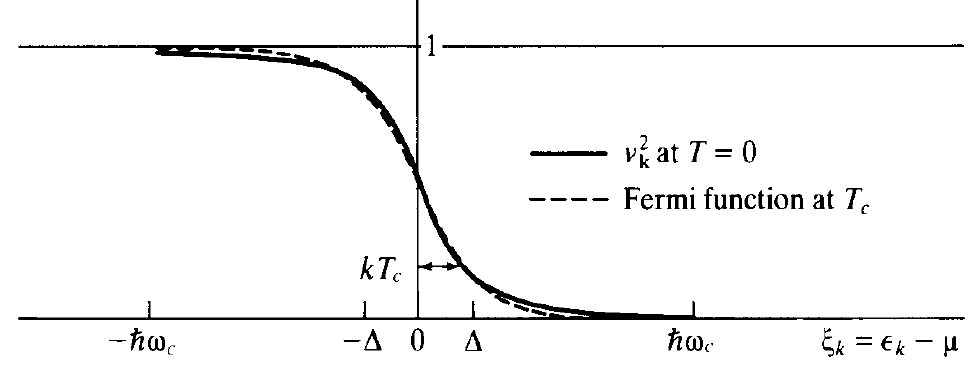
\includegraphics[width=0.8\textwidth]{immagini/andamento_nu_quadro.png}
\end{figure}
\hspace{-0.6cm}La parte sinistra dell'asse orizzontale corrisponde a valori negativi di $\xi(\vb{k})$, cioè energie inferiori al livello di Fermi, mentre la parte destra corrisponde a energie superiori.\\
Il comportamento di questo coefficiente fornisce informazioni importanti: nel sottospazio di Nambu associato a $\vb{k}$, $|\nu_{\vb{k}}|^2$ rappresenta la probabilità di trovare una coppia di elettroni (cioè una coppia di Cooper) con quella combinazione di momento e spin.\\
Analizziamo i regimi asintotici. Per $\varepsilon(\vb{k})<\mu$, cioè sotto il livello di Fermi, i livelli sono occupati nello stato normale, e infatti $|\nu_{\vb{k}}|^2 \to 1$. Per $\varepsilon(\vb{k})>\mu$, invece, i livelli sono vuoti e $|\nu_{\vb{k}}|^2 \to 0$.\\
Nella regione intermedia, dell'ordine di $\Delta$, la funzione presenta una transizione smussata, molto simile alla distribuzione di Fermi--Dirac a temperatura finita (indicata nel grafico con una linea tratteggiata).\\
È importante sottolineare che, nonostante la somiglianza, si tratta di quantità fisicamente diverse: da un lato abbiamo la probabilità di trovare una coppia di Cooper nello stato fondamentale BCS, dall'altro la probabilità di occupazione di uno stato a singola particella in un metallo normale a temperatura finita.\\
Questa somiglianza suggerisce però che gli stati elettronici rilevanti nello stato BCS sono quelli vicini al livello di Fermi, analogamente a quanto accade nel gas di Fermi a temperatura finita.\\
Questo è ragionevole, poiché la superconduttività emerge a una temperatura critica: gli elettroni che partecipano alla transizione sono proprio quelli vicini al livello di Fermi.\\
Tuttavia, esiste una differenza fondamentale: nello stato normale gli elettroni occupano stati indipendenti, senza coerenza di fase, mentre nello stato fondamentale BCS abbiamo una sovrapposizione coerente di stati a molti corpi. In questo caso non contano solo i moduli dei coefficienti, ma anche le loro fasi.\mn{Nel caso dello stato fondamentale BCS, a differenza del gas di Fermi normale, gli osservabili dipendono da combinazioni lineari dei coefficienti (come nel caso di $\expval*{\hat{\Delta}}$ che dipende da $u_{\vb{k}} \nu_{\vb{k}}^*$) e non solo dai loro moduli quadrati. Questo implica che le fasi relative dei coefficienti giocano un ruolo fisico fondamentale.}\\
In altre parole, lo stato fondamentale BCS è una sovrapposizione coerente di stati a molti corpi: una combinazione macroscopica con coerenza di fase. Questo è il senso in cui si dice che lo stato fondamentale BCS è uno stato coerente macroscopico.

\section{Lo stato coerente macroscopico}

Vediamo cosa significa affermare che lo stato fondamentale BCS è uno stato coerente macroscopico. Il termine macroscopico è intuitivo: deriva dal fatto che il sistema contiene un numero molto grande di particelle. Il termine coerente, invece, richiede qualche spiegazione.\\
Per prima cosa riscriviamo lo stato fondamentale BCS in una forma che permetta un confronto più immediato con uno stato coerente bosonico. Ricordiamo la sua espressione:
\begin{equation*}
   \ket{g_s}
   =\prod_{\vb{k}} \qty( u_{\vb{k}} \ket{0_{\vb{k}}} + \nu_{\vb{k}} \ket{2_{\vb{k}}} )
   =\prod_{\vb{k}} \qty( u_{\vb{k}} + \nu_{\vb{k}} Z^\dagger_{\vb{k}} ) \ket{0}
\end{equation*}
Possiamo riscriverlo come
\begin{equation*}
   \ket{g_s}
   =\prod_{\vb{k}} u_{\vb{k}} \qty( 1 + \frac{\nu_{\vb{k}}}{u_{\vb{k}}} Z^\dagger_{\vb{k}} ) \ket{0}
   = \text{cost.} \times \prod_{\vb{k}} \qty( 1 + \alpha_{\vb{k}} Z^\dagger_{\vb{k}} ) \ket{0}
\end{equation*}
dove abbiamo definito $\alpha_{\vb{k}}=\frac{\nu_{\vb{k}}}{u_{\vb{k}}}$ e la costante è data dal prodotto di tutti gli $u_{\vb{k}}$.\\
Ora cerchiamo di esprimere $u_{\vb{k}}$ e $\nu_{\vb{k}}$ in funzione di $\alpha_{\vb{k}}$. Dalla condizione di normalizzazione si ha
\begin{equation*}
   |u_{\vb{k}}|^2 + |\nu_{\vb{k}}|^2
   =|u_{\vb{k}}|^2 \qty( 1 + \frac{|\nu_{\vb{k}}|^2}{|u_{\vb{k}}|^2} )
   =|u_{\vb{k}}|^2 \qty( 1 + |\alpha_{\vb{k}}|^2 )
   =1
\end{equation*}
da cui segue
\begin{equation*}
   |u_{\vb{k}}|^2
   =\frac{1}{ 1 + |\alpha_{\vb{k}}|^2 }
   \qq{;}
   |\nu_{\vb{k}}|^2
   =\frac{ |\alpha_{\vb{k}}|^2 }{ 1 + |\alpha_{\vb{k}}|^2 }
\end{equation*}
Inoltre, l'operatore $\bigl( 1 + \alpha_{\vb{k}} Z^\dagger_{\vb{k}} \bigr)$ può essere riscritto come un esponenziale:\mn{Si presti attenzione al fatto che questa uguaglianza non vale in generale, ma perché $Z^\dagger_{\vb{k}}$ è costruito a partire da operatori fermionici, dunque soddisfa la relazione
\begin{equation*}
   \bigl(Z^\dagger_{\vb{k}}\bigr)^2 = 0
\end{equation*}
Di conseguenza, lo sviluppo in serie dell'esponenziale
\begin{equation*}
   e^{\alpha_{\vb{k}} Z^\dagger_{\vb{k}}}
   =\sum_{n=0}^{\infty} \frac{ (\alpha_{\vb{k}} Z^\dagger_{\vb{k}})^n }{n!}
\end{equation*}
si tronca automaticamente al primo ordine.}
\begin{equation*}
   1 + \alpha^{\vphantom{\dag}}_{\vb{k}} Z^\dagger_{\vb{k}}
   =e^{\alpha^{\vphantom{\dag}}_{\vb{k}} Z^\dagger_{\vb{k}}}
\end{equation*}
dunque lo stato fondamentale può essere riscritto come
\begin{equation}
   \ket{g_s}
   =\text{cost.} \times \prod_{\vb{k}} e^{\alpha_{\vb{k}} Z^\dagger_{\vb{k}}} \ket{0}
   =\text{cost.} \times \exp \Bigl( \sum_{\vb{k}} \alpha^{\vphantom{\dag}}_{\vb{k}} Z^\dagger_{\vb{k}} \Bigr) \ket{0}
   \label{eq:BCS_ground_state_forma_stato_coerente}
\end{equation}
A questo punto scriviamo l'espressione di uno stato coerente bosonico.\\
Uno stato coerente bosonico è uno stato $\ket*{\alpha}$ definito come
\begin{equation*}
   \ket*{\alpha}
   =\text{cost.} \times e^{\alpha a^{\dag}} \ket{0}
\end{equation*}
Questa espressione ha una forma molto simile a quella dello stato BCS, poiché $a^{\dag}$ è l'operatore di creazione bosonico. Tuttavia, bisogna prestare attenzione: si tratta di quantità diverse, a causa delle differenti statistiche. Infatti, $a^{\dag}$ è un operatore bosonico, mentre $Z^{\dag}_{\vb{k}}$ è un operatore composto da due operatori fermionici, e quindi non valgono le regole di commutazione bosoniche.\\
Nonostante ciò, possiamo osservare che i due stati hanno una struttura matematica molto simile.\\
L'obiettivo ora è capire perché questa analogia sia rilevante: non si tratta soltanto di una somiglianza formale, ma del fatto che alcune proprietà degli stati coerenti bosonici possono essere utilizzate per comprendere proprietà analoghe dello stato fondamentale BCS.
\subsection{Stati coerenti}
Facciamo adesso un breve ripasso sugli stati bosonici coerenti. Per tale scopo, consideriamo l'oscillatore armonico quantistico. L'operatore hamiltoniano di tale sistema è dato da
\begin{equation*}
   \hat{H} = \frac{\hat{p}^2}{2m} + \frac{m\omega^2}{2} \hat{x}^2
\end{equation*}
Gli autostati dell'oscillatore sono dati da
\begin{equation}
   \hat{H} \ket*{n} = E_n \ket*{n}
\end{equation}
dove $E_n$ sono i livelli energetici.\\
Il metodo più elegante per risolvere questo problema , ovvero per determinare energie ed autostati, consiste nell'introdurre gli operatori di creazione e distruzione, $a^{\dag}$ e $a$, mediante i quali possiamo esprimere gli operatori di posizione e momento come
\begin{equation*}
   \hat{x}=\text{cost.} \times (a + a^{\dag})
   \qq{;}
   \hat{p}=\text{cost.} \times (a^{\dag} - a)
\end{equation*}
con le costanti scelte in modo opportuno.\\
Tali operatori sono degli operatori bosonici e possiedono una serie di proprietà molto utili. Innanzitutto per essi vale la relazione di commutazione
\begin{equation}
   [a^{\dag}, a] = 1
   \label{eq:bosonic_commutation_relation}
\end{equation}
Inoltre, l'azione dell'operatore di creazione $a^{\dag}$ su uno stato di Fock, cioè uno stato con $n$ bosoni, è data da
\begin{equation*}
   a^{\dag} \ket{n} = \sqrt{n+1} \ket{n+1}
\end{equation*}
mentre l'azione dell'operatore di annichilazione è
\begin{equation*}
   a \ket{n} = \sqrt{n} \ket{n-1}
\end{equation*}
Possiamo definire l'operatore numero $\hat{n} = a^{\dag} a$, la cui azione su uno stato di Fock è
\begin{equation*}
   \hat{n} \ket{n} = n \ket{n}
\end{equation*}
In termini di questi operatori, l'Hamiltoniana dell'oscillatore è data da
\begin{equation*}
   \hat{H} = \hbar \omega \left( a^{\dag} a + \frac{1}{2} \right)
\end{equation*}
e in tale forma si ottiene immediatamente che i livelli energetici sono
\begin{equation*}
   E_n = \hbar \omega \left( n + \frac{1}{2} \right)
\end{equation*}
Per come agisce l'operatore di creazione $a^{\dag}$ su uno stato di Fock, è possibile costruire tutti gli autostati $\ket*{n}$ in modo iterativo, agendo ripetutamente sullo stato fondamentale iniziale $\ket{0}$:
\begin{equation}
   \ket*{n}=\frac{1}{\sqrt{n!}} {(a^{\dag})}^n \ket{0}
   \label{eq:formula_ricorsiva_autostati_oscillatore}
\end{equation}
Tali operatori hanno anche molti altri utilizzi. In particolare, definiamo uno stato coerente come
\begin{equation}
   \ket{\alpha} 
   = C \qty(
   \ket*{0}
   + \frac{\alpha}{\sqrt{1!}} \ket*{1}
   + \frac{\alpha^2}{\sqrt{2!}} \ket*{2}
   + \ldots )
   \label{eq:coherent_state}
\end{equation}
dove $\alpha$ è un numero complesso arbitrario e $C$ è una costante di normalizzazione. Quest'ultima può essere determinata dalla condizione di normalizzazione
\begin{equation*}
   1 = \braket*{\alpha}
   = |C|^2 \left( 1 + \frac{|\alpha|^2}{1!} + \frac{{(|\alpha|^2)}^2}{2!} + \ldots \right)
   = |C|^2 e^{|\alpha|^2}
\end{equation*}
da cui si ottiene
\begin{equation*}
   C = e^{-|\alpha|^2/2}
\end{equation*}
Gli stati coerenti possiedono molte proprietà interessanti. Notiamo innanzitutto che l'\eqrefcustom{eq:coherent_state} può essere riscritta in termini dell'operatore di creazione $a^{\dag}$. Utilizzando l'\eqrefcustom{eq:formula_ricorsiva_autostati_oscillatore} per ciascun termine si ha
\begin{equation*}
   \ket*{\alpha}
   = e^{-|\alpha|^2/2} \left( 1 + \frac{\alpha a^{\dag}}{1!} + \frac{(\alpha a^{\dag})^2}{2!} + \ldots \right) \ket*{0}
\end{equation*}
dove $\ket*{0}$ è lo stato fondamentale ed è anche lo stato coerente con $\alpha = 0$. Questa espressione può essere scritta in forma molto compatta come
\begin{equation*}
\ket*{\alpha} = e^{-|\alpha|^2/2} e^{\alpha a^{\dag}} \ket*{0}
\end{equation*}
dove abbiamo usato la definizione dell'esponenziale di un operatore $\hat{X}$ tramite lo sviluppo in serie
\begin{equation*}
   e^{\hat{X}} = 1 + \frac{\hat{X}}{1!} + \frac{\hat{X}^2}{2!} + \ldots
\end{equation*}
Un'altra relazione interessante, che può essere ottenuta dall'\eqrefcustom{eq:coherent_state}, è
\begin{equation}
   a \ket*{\alpha} = \alpha \ket*{\alpha}
   \label{eq:coherent_state_eigenvalue_equation}
\end{equation}
ovvero gli stati coerenti sono autostati dell'operatore di annichilazione $a$. Per dimostrarlo possiamo scrivere esplicitamente lo stato $a\ket*{\alpha}$:
\begin{equation*}
   a\ket*{\alpha}
   = e^{-|\alpha|^2/2} \, a
   \qty( \ket*{0} + \frac{\alpha}{\sqrt{1!}} \ket*{1} + \frac{\alpha^2}{\sqrt{2!}} \ket*{2} + \ldots )
\end{equation*}
Ma poiché $a\ket*{n} = \sqrt{n}\ket*{n-1}$, si ottiene
\begin{equation*}
   a\ket*{\alpha} = e^{-|\alpha|^2/2} \left( 0 + \frac{\alpha \sqrt{1}}{\sqrt{1!}} \ket*{0} + \frac{\alpha^2 \sqrt{2}}{\sqrt{2!}} \ket*{1} + \ldots \right)
\end{equation*}
che è chiaramente uguale a $\alpha \ket*{\alpha}$.\\
Infine, dall'\eqrefcustom{eq:coherent_state_eigenvalue_equation} segue che
\begin{equation*}
   \mel*{\alpha}{a^{\dag} a}{\alpha}
   =\bigl( \bra*{\alpha} a^{\dag} \bigr) \bigl( a \ket*{\alpha} \bigr)
   =\alpha^* \alpha \braket*{\alpha}
   = |\alpha|^2
\end{equation*}
Pertanto, il valore di $|\alpha|^2$ fornisce il valore medio dell'operatore numero $\expval*{\hat{n}}$ dello stato quantistico.\\
Estendendo questo risultato a $\hat{n}^2$ possiamo determinare l'incertezza sul numero $\Delta n$. Calcoliamo quindi $\expval*{\hat{n}^2}$:
\begin{equation*}
   \expval*{\hat{n}^2} = \mel*{\alpha}{a^{\dag} a a^{\dag} a}{\alpha}
\end{equation*}
dall'\eqrefcustom{eq:bosonic_commutation_relation} si ha che
\begin{equation*}
   [a^{\dag}, a] = a^{\dag} a - a a^{\dag} = 1
   \implies
   a a^{\dag} = a^{\dag} a + 1
\end{equation*}
Inserendo tale risultato precedenti, si ottiene
\begin{equation*}
   \expval*{\hat{n}^2}
   =\mel*{\alpha}{a^{\dag}(a^{\dag} a + 1) a }{\alpha}
   =\mel*{\alpha}{a^{\dag}a^{\dag} a a }{\alpha}
   + \mel*{\alpha}{a^{\dag} a}{\alpha}
\end{equation*}
Il secondo termine non è altro che $\expval*{\hat{n}}$, che abbiamo già calcolato essere $|\alpha|^2$. Per quanto riguarda il primo termine, possiamo riscriverlo come
\begin{equation*}
   \mel*{\alpha}{a^{\dag}a^{\dag} a a }{\alpha}
   =\bigl( \bra*{\alpha} a^{\dag}a^{\dag} \bigr) \bigl( a a \ket*{\alpha} \bigr)
\end{equation*}
Dato che vale l'\eqrefcustom{eq:coherent_state_eigenvalue_equation}, si ha che $a a \ket*{\alpha} = \alpha^2 \ket*{\alpha}$, e in maniera analoga $\bra*{\alpha} a^{\dag}a^{\dag} = {(\alpha^*)}^2 \bra*{\alpha}$, quindi
\begin{equation*}
   \mel*{\alpha}{a^{\dag}a^{\dag} a a }{\alpha}
   =|\alpha|^4
\end{equation*}
In definitiva abbiamo trovato che
\begin{equation*}
   \expval*{\hat{n}^2} = |\alpha|^4 + |\alpha|^2
\end{equation*}
Una volta calcolati $\expval*{\hat{n}}$ e $\expval*{\hat{n}^2}$, possiamo calcolare l'incertezza $\Delta n$:
\begin{equation*}
   \Delta n
   = \sqrt{\expval*{\hat{n}^2} - \expval*{\hat{n}}^2}
   = |\alpha|
\end{equation*}
Ora vogliamo determinare quale sia la relazione tra il numero medio di bosoni nello stato coerente e la sua varianza, in modo da poter valutare quale sia l'incertezza sul numero di bosoni nello stato coerente. Si ha che
\begin{equation}
   \frac{\Delta n}{\expval*{\hat{n}}}
   =\frac{|\alpha|}{|\alpha|^2}
   =\frac{1}{|\alpha|}
\end{equation}
Saremo principalmente interessati a stati coerenti macroscopici, per i quali $\expval*{\hat{n}}$, e quindi $|\alpha|$, è molto grande. Per tali stati, si può vedere che la deviazione standard $\Delta n$ diventa trascurabile rispetto a $\expval*{\hat{n}}$. Pertanto, come buona approssimazione, possiamo approssimare molti valori medi di operatori con i loro valori di campo medio ottenuti dalla sostituzione $\hat{n} \approx \expval*{\hat{n}}$.\\
Questo è, in un certo senso, qualcosa di simile a quanto abbiamo già visto per lo stato fondamentale BCS, che presenta una struttura in cui il numero medio di elettroni è molto grande, ma l'incertezza relativa è molto piccola. In questo senso esiste un'analogia, che deriva anche dalla struttura degli stati.\\
È importante notare che lo stato coerente $\ket*{\alpha}$ possiede una fase $\vartheta$ ben definita, pur non avendo un numero quantico $n$ definito. Infatti, il numero complesso $\alpha$ che descrive lo stato coerente può essere espresso come
\begin{equation*}
   \alpha = |\alpha| e^{i\vartheta}
\end{equation*}
e esprimendolo in tale forma all'interno dell'\eqrefcustom{eq:coherent_state} si ottiene
\begin{equation}
   \ket*{\alpha}
   = e^{-|\alpha|^2/2} 
   \qty( \ket*{0} + \frac{|\alpha| e^{i\vartheta}}{\sqrt{1!}} \ket*{1} + \frac{|\alpha|^2 e^{i2\vartheta}}{\sqrt{2!}} \ket*{2} + \ldots )
   \label{eq:coherent_state_polar_form}
\end{equation}
Si vede che il termine contenente $\ket*{n}$ dipende da $e^{in\vartheta}$. Ciò non ci sorprende in quanto, come abbiamo visto, gli stati coerenti sono sovrapposizioni di stati di Fock con numeri quantici $n$ diversi, e ciascuno di questi stati di Fock contribuisce con una fase.\\
Derivando l'\eqrefcustom{eq:coherent_state_polar_form} rispetto a $\vartheta$ si ottiene
\begin{equation*}
   \pdv{}{\vartheta} \ket*{\alpha}
   = e^{-|\alpha|^2/2} \qty( 0 + \frac{i |\alpha| e^{i\vartheta}}{\sqrt{1!}} \ket*{1} + \frac{2i |\alpha|^2 e^{i2\vartheta}}{\sqrt{2!}} \ket*{2} + \ldots )
\end{equation*}
Da cui si ricava
\begin{equation*}
   \frac{1}{i}\frac{\partial}{\partial \vartheta} \ket*{\alpha} = \hat{n} \ket*{\alpha}
\end{equation*}
Poiché gli stati $\ket*{\alpha}$ costituiscono un insieme completo (in realtà sovracompleto), possiamo effettuare l'identificazione tra operatori
\begin{equation*}
   \frac{1}{i}\frac{\partial}{\partial \vartheta} = \hat{n}
\end{equation*}
Pertanto, la fase $\vartheta$ e il numero $n$ sono operatori coniugati, in modo analogo a quanto accade per quantità di moto e posizione nella meccanica quantistica standard. Di conseguenza, è possibile formulare una relazione di indeterminazione per questi operatori:
\begin{equation*}
   \Delta n \, \Delta \vartheta \geq \frac{1}{2}
\end{equation*}
Gli stati coerenti hanno una fase ben definita, ma non possiedono un valore definito del numero quantico $n$. Al contrario, gli autostati di energia $\ket*{n}$ hanno un valore ben definito di $n$, ma una fase arbitraria (o indefinita).
\section{Proprietà dello stato fondamentale BCS}
\subsection{Rottura della simmetria di gauge}
Vediamo quali sono le implicazioni per lo stato fondamentale BCS.\\
La nostra osservazione iniziale è stata che lo stato fondamentale può essere scritto nella forma dell'\eqrefcustom{eq:BCS_ground_state_forma_stato_coerente}, che ha la stessa struttura di uno stato coerente bosonico. In questo senso, si tratta di uno stato coerente, ma di coppie di Cooper, poiché l'operatore $\hat{Z}^{\dag}$ crea coppie di Cooper.\\
Inoltre, in analogia con uno stato coerente bosonico, che possiede un valore definito di $\alpha$, anche lo stato coerente fermionico, almeno in ciascun sottospazio di Nambu per ogni $\vb{k}$, possiede una fase ben definita. Questa fase definita, analogamente al caso bosonico, implica un'incertezza nel numero di particelle, che in questo caso sono fermioni.\\
Il passo che stiamo compiendo ora consiste nel prendere l'analogia tra numero di particelle e fase che vale per gli stati coerenti e applicarla allo stato BCS.\\
Fissare $\alpha_{\vb{k}}$ significa fissare la fase relativa tra $\nu_{\vb{k}}$ e $u_{\vb{k}}$, cioè tra le componenti con zero e due elettroni. Tuttavia, una variazione di questa fase non modifica $|\Delta|$, che entra nel valore medio dell'energia nello stato BCS.\\
Questo significa che cambiando la fase di $\alpha_{\vb{k}}$ otteniamo stati con fasi diverse, ma energeticamente degeneri. Tuttavia, quando avviene la transizione e il sistema è descritto dallo stato fondamentale BCS, esso seleziona uno specifico valore di $\alpha_{\vb{k}}$, cioè coefficienti ben determinati. In altre parole, il sistema sceglie un valore specifico della fase.\\
Abbiamo quindi una famiglia di stati, tutti degeneri, corrispondenti a diversi valori di $\alpha_{\vb{k}}$, ma il sistema ne seleziona uno solo. Questo è precisamente ciò che si intende per rottura spontanea di simmetria, e la simmetria che viene rotta in questo caso è una simmetria di gauge.\\
Per riassumere, stiamo collegando le proprietà dello stato fondamentale BCS alla rottura della simmetria di gauge nella transizione superconduttiva. Abbiamo già introdotto questo concetto dal punto di vista della teoria di Ginzburg-Landau, ma qui lo vediamo emergere direttamente dalla struttura dello stato fondamentale BCS.\\
La struttura dello stato fondamentale BCS, espressa come stato coerente fermionico, è
\begin{equation*}
   \ket{g_s}
   =\text{cost.} \times \exp \Bigl( \sum_{\vb{k}} \alpha_{\vb{k}} Z^\dagger_{\vb{k}} \Bigr) \ket{0}
\end{equation*}
dove $\hat{Z}^{\dag}_{\vb{k}}$ è l'operatore che crea una coppia di elettroni con struttura di coppia di Cooper.\\
Inoltre, abbiamo derivato la forma dei coefficienti $u_{\vb{k}}$ e $\nu_{\vb{k}}$ e, in particolare, dobbiamo ricordare che il loro prodotto è semplicemente legato a $\Delta$, che è il valore medio dell'operatore $\hat{Z}_{\vb{k}}$, tramite l'\eqrefcustom{eq:BCS_u_nu_Delta_relation}.\\
Abbiamo anche visto che il valore medio dell'hamiltoniana BCS, meno il contributo introdotto per tenere conto del fatto che il numero di particelle non è fissato, valutato sullo stato fondamentale, è dato dall'\eqrefcustom{eq:BCS_energy}:
\begin{equation*}
   \mel*{g_s}{H - \mu N}{g_s}=\sum_{\vb{k}} 2 \xi(\vb{k}) |\nu_{\vb{k}}|^2 + V \Bigl| \sum_{\vb{k}} u_{\vb{k}} \nu^*_{\vb{k}} \Bigr|^2
\end{equation*}
Per quanto riguarda il primo termine, definendo
\begin{equation*}
   E_{\vb{k}}=\sqrt{\xi^2_{\vb{k}} + |\Delta|^2}
\end{equation*}
e inserendo l'\eqrefcustom{eq:coefficiente_nu_BCS} si ottiene
\begin{equation*}
   2 \sum_{\vb{k}} \xi_{\vb{k}} |\nu_{\vb{k}}|^2
   = 2 \sum_{\vb{k}} \xi_{\vb{k}} \frac{1}{2} \qty( 1 - \frac{\xi_{\vb{k}}}{E_{\vb{k}}} )
   = \sum_{\vb{k}} \qty( \xi_{\vb{k}} - \frac{\xi^2_{\vb{k}}}{E_{\vb{k}}} )
\end{equation*}
Per il secondo termine, invece, dalle definizioni di $\Delta$ e $\Delta^*$ segue che
\begin{equation*}
   V \Bigl| \sum_{\vb{k}} u_{\vb{k}} \nu^*_{\vb{k}} \Bigr|^2
   =\frac{|\Delta|^2}{V}
   =-\frac{|\Delta|^2}{|V|}
\end{equation*}
In definitiva
\begin{equation}
   \mel*{g_s}{H - \mu N}{g_s}
   = \sum_{\vb{k}} \qty( \xi_{\vb{k}} - \frac{\xi^2_{\vb{k}}}{E_{\vb{k}}} ) - \frac{|\Delta|^2}{|V|}
   \label{eq:BCS_energy_final_expression}
\end{equation}
Si noti che la somma è estesa a tutti i valori di $\vb{k}$ e non solo a quelli sopra o sotto il momento di Fermi.\\
A partire da qui, facciamo alcune osservazioni e colleghiamo queste proprietà alla rottura della simmetria di gauge. Innanzitutto, $\Delta$ è in generale una quantità complessa, quindi possiamo scrivere
\begin{equation*}
   \Delta = |\Delta| e^{i\phi}
\end{equation*}
Osserviamo che l'energia è reale e dipende solo da $|\Delta|^2$, mentre i coefficienti $u_{\vb{k}}$ e $\nu_{\vb{k}}$, che possono essere complessi, dipendono da $\Delta$. Ciò implica che, variando la fase di $\Delta$, si ottengono coefficienti $u_{\vb{k}}$ e $\nu_{\vb{k}}$ diversi. In particolare, tutti i coefficienti cambiano fase nello stesso modo, cioè questa fase non dipende da $\vb{k}$. Di conseguenza, la fase relativa tra i coefficienti che definiscono le coppie di Cooper è la stessa per tutti gli stati.\\
Questo significa che valori diversi del parametro complesso $\Delta$ corrispondono a stati diversi, poiché cambiano i coefficienti della sovrapposizione che definisce lo stato fondamentale, ma tutti questi stati hanno la stessa energia. Quindi tutti gli stati che differiscono per una fase globale, comune a tutti i $\vb{k}$, sono degeneri. Ciò porta naturalmente alla rottura di una simmetria: se il sistema si trova in uno stato fondamentale con una fase specifica, pur esistendo infiniti stati degeneri con la stessa energia, significa che è stata effettuata una scelta tra stati equivalenti. Questo è analogo a quanto accade nella transizione ferromagnetica, dove il sistema sceglie una direzione di magnetizzazione tra infinite direzioni energeticamente equivalenti.\\
Tale fatto è quindi un chiaro segnale dell'avvenire di una transizione. Il tipo di simmetria che viene rotta, come già anticipato, è la simmetria di gauge.\\
Richiamiamo brevemente quale tipo di simmetria di gauge abbiamo considerato. Per una singola particella, possiamo avere una trasformazione di gauge globale o locale. Una trasformazione globale consiste nel moltiplicare la funzione d'onda $\psi$ per una fase costante:
\begin{equation*}
   \psi \rightarrow e^{i\chi} \psi
\end{equation*}
Questi stati sono fisicamente equivalenti, riflettendo l'ambiguità di fase intrinseca della meccanica quantistica.\\
Possiamo anche considerare una trasformazione di gauge locale, in cui la fase dipende da spazio e tempo:
\begin{equation*}
   \psi(\vb{r},t)
   \longrightarrow
   \psi(\vb{r},t) e^{i \frac{q \chi(\vb{r},t)}{\hbar}}
   \equiv \tilde{\psi}(\vb{r},t)
\end{equation*}
Se $\psi$ soddisfa l'equazione di Schrödinger
\begin{equation*}
   i \hbar \pdv{\psi}{t}
   =-\frac{\hbar^2}{2m} \laplacian{\psi}
\end{equation*}
allora $\tilde{\psi}$ soddisfa l'equazione modificata
\begin{equation*}
   i \hbar \pdv{\tilde{\psi}}{t}
   =\qty[ -\frac{\hbar^2}{2m} \qty( \grad - i \frac{q}{\hbar} \vb{A} )^2 + q\Phi ] \tilde{\psi}
   \qq{dove}
   \begin{dcases}
   \Phi = -\pdv{\chi}{t}
   \\
   \vb{A} = \grad \chi
   \end{dcases}
\end{equation*}
Consideriamo ora un sistema a molte particelle, in particolare lo stato fondamentale BCS. Partiamo dallo stato di Fock $\ket*{\{ n_{\vb{k}} \} }$, dove $n_k$ è il numero di occupazione del livello $k$, che per i fermioni può essere 0 o 1. Se applichiamo una trasformazione di fase globale a ciascuna particella, ogni stato $\ket*{n_k}$ diventa $e^{i\chi} \ket*{n_k}$, e lo stato complessivo acquista una fase globale:
\begin{equation*}
   \ket*{\{ n_{\vb{k}} \} }
   \longrightarrow
   e^{i N \chi} \ket*{\{ n_{\vb{k}} \} }
\end{equation*}
dove $N$ è il numero totale di elettroni.\\
Poiché $n_k$ sono autovalori dell'operatore numero $\hat{n}_k = c_k^\dagger c_k$, possiamo ottenere questo effetto modificando gli operatori di creazione:
\begin{equation*}
   c_k^\dagger \longrightarrow e^{i\chi} c_k^\dagger
\end{equation*}
Questa trasformazione non modifica l'operatore numero, poiché il fattore di fase si cancella con quello dell'hermitiano coniugato. In altre parole, le osservabili restano invarianti, come richiesto.
\subsection{Relazione di indeterminazione fase--numero}
Vediamo cosa accade allo stato fondamentale BCS se effettuiamo una trasformazione di fase globale su ciascuno degli elettroni che partecipano allo stato. Ricordiamo la forma dello stato, descritta dall'\eqrefcustom{eq:BCS_trial_wavefunction_Nambu}:
\begin{equation*}
   \ket{\psi_g}
   =\prod_{\vb{k}} \bigl( u_{\vb{k}} + \nu_{\vb{k}} \hat{Z}^{\dag}_{\vb{k}} \bigr) \ket*{\phi_0}
\end{equation*}
Ricordiamo inoltre che $\hat{Z}^{\dag}_{\vb{k}}$ è il prodotto di due operatori di creazione relativi a due elettroni con la corretta combinazione di momento e spin, cioè $c^{\dag}_{\vb{k},\uparrow} c^{\dag}_{-\vb{k},\downarrow}$. Se modifichiamo ciascun operatore di creazione introducendo il fattore di fase, allora l'operatore di creazione di coppia si trasforma nel modo seguente:
\begin{equation*}
   \hat{Z}^{\dag}_{\vb{k}}
   \longrightarrow
   e^{2i\chi} \hat{Z}^{\dag}_{\vb{k}}
\end{equation*}
Ciò implica che lo stato fondamentale BCS si trasforma in
\begin{equation*}
   \ket{\psi_g}
   \longrightarrow
   \ket*{\psi_{\chi}}
   =
   \prod_{\vb{k}=\vb{k}_1,\ldots,\vb{k}_M}
   \bigl(
      u_{\vb{k}}
      +
      \nu_{\vb{k}} e^{2i\chi}
      c^{\dag}_{\vb{k},\uparrow}
      c^{\dag}_{-\vb{k},\downarrow}
   \bigr)\ket*{0}
\end{equation*}
Se osserviamo questo stato senza preoccuparci momentaneamente della sua origine, possiamo interpretare questa trasformazione come una modifica della fase relativa tra $u_{\vb{k}}$ e $\nu_{\vb{k}}$, ed è proprio questo il punto che avevamo anticipato in precedenza: stiamo modificando la fase relativa tra questi coefficienti senza alterare l'energia dello stato. Ciò significa che lo stato $\ket*{\psi_{\chi}}$ appartiene alla famiglia di stati degeneri di cui abbiamo parlato in precedenza. In altre parole, i diversi stati fondamentali aventi la stessa energia ma differente fase possono essere scritti in questa forma. Quando il sistema seleziona uno stato particolare, esso sceglie una fase definita. Questo corrisponde alla rottura della simmetria di gauge, poiché si tratta esattamente dello stesso tipo di trasformazione di gauge globale discusso in precedenza.\\
Avere una fase definita corrisponde però a non avere un numero di particelle ben definito. Compare infatti una relazione di indeterminazione tra fase e numero di particelle, analoga a quella tra posizione e quantità di moto. Questo può essere visto facilmente partendo da uno stato generico $\ket*{\psi_{\chi}}$. Poiché sappiamo che si tratta di uno stato a molte particelle, possiamo scriverlo come sovrapposizione di stati a numero fissato di particelle:
\begin{equation*}
   \ket*{\psi_{\chi}}
   =
   \sum_N
   \lambda_N e^{i N \chi}
   \ket*{\psi_N}
\end{equation*}
I coefficienti $\lambda_N$ sono incogniti e, in linea di principio, possono essere determinati a partire dalla forma esplicita dello stato fondamentale BCS. Inoltre, sappiamo che ciascuno stato $\ket*{\psi_N}$ deve acquisire una fase del tipo $e^{i N \chi}$, proprio perché deriva dalla trasformazione dello stato BCS. Questa scrittura rappresenta quindi un modo formale di descrivere lo stato BCS come uno stato a molte particelle in cui le coppie possono essere occupate oppure no, ma mantenendo una relazione di fase ben definita tra le componenti con diverso numero di particelle, cioè una coerenza quantistica tra tali componenti.\\
Possiamo ora chiederci se sia possibile estrarre dallo stato fondamentale BCS la componente con numero fissato di particelle. In altre parole, dato uno stato generale della forma
\begin{equation*}
   \ket*{\psi}
   =
   \sum_i a_i \ket*{\psi_i}
\end{equation*}
possiamo domandarci se sia possibile determinare il peso $|a_i|^2$ dei vari stati oppure verificare se un certo stato $\ket*{\psi_j}$ appartenga alla sovrapposizione.\\
Normalmente, ciò che si fa è proiettare lo stato sul vettore desiderato. Se $\ket*{\psi_j}$ appartiene alla base dello spazio di Hilbert, allora:
\begin{equation*}
   \braket*{\psi_j}{\psi}
   =\sum_i a_i \braket*{\psi_j}{\psi_i}
   =a_j
\end{equation*}
Nel caso dello stato fondamentale BCS, possiamo sfruttare la decomposizione in stati a numero fissato di particelle e moltiplicare $\ket*{\psi_{\chi}}$ per una fase $e^{-i \bar{N} \chi}$:
\begin{equation*}
   e^{-i \bar{N} \chi}
   \ket*{\psi_{\chi}}
   =
   \sum_N
   \lambda_N
   e^{i\chi (N-\bar{N})}
   \ket*{\psi_N}
\end{equation*}
Poiché $\chi$ è un parametro libero, possiamo integrare tale espressione rispetto ad esso:
\begin{equation*}
   \int_0^{2\pi}
   \dd{\chi}\,
   e^{-i \bar{N} \chi}
   \ket*{\psi_{\chi}}
   =
   \sum_N
   \lambda_N
   \ket*{\psi_N}
   \int_0^{2\pi}
   \dd{\chi}\,
   e^{i\chi(N-\bar{N})}
\end{equation*}
Ma l'integrale della funzione esponenziale è nullo per tutti i valori di $N$ diversi da $\bar{N}$,\mn{Ricordiamo infatti che
\begin{equation*}
   \int_0^{2\pi}
   \dd{x}\,
   e^{ix(\alpha-\alpha')}
   =
   2\pi \delta_{\alpha,\alpha'}
\end{equation*}
}
quindi otteniamo
\begin{equation*}
   \int_0^{2\pi}
   \dd{\chi}\,
   e^{-i \bar{N} \chi}
   \ket*{\psi_{\chi}}
   =
   2\pi \lambda_{\bar{N}}
   \ket*{\psi_{\bar{N}}}
\end{equation*}
L'integrale seleziona quindi esclusivamente la componente con numero di particelle pari a $\bar{N}$. Dal punto di vista matematico questo passaggio è piuttosto semplice, ma il suo significato fisico è molto importante. Se vogliamo estrarre dallo stato fondamentale BCS la componente a numero fissato di particelle, dobbiamo rendere completamente indeterminata la fase $\chi$ che caratterizza lo stato, poiché stiamo integrando su tutti i valori possibili di $\chi$ tra $0$ e $2\pi$. Questo mostra che lo stato fondamentale BCS è uno stato a fase definita ma con numero di particelle non definito. Si tratta quindi di una manifestazione della relazione di indeterminazione tra fase e numero di particelle, nella teoria BCS sono due variabili coniugate, e se vogliamo fissare una di esse, l'altra diventa completamente indeterminata.\\
Questa osservazione è importante perché ci si potrebbe chiedere quale sia il significato fisico di uno stato con numero di particelle non fissato. Una descrizione di questo tipo sarebbe infatti priva di senso per un sistema contenente poche particelle. Tuttavia, nel caso di un superconduttore macroscopico, il numero di particelle è enorme, e in questa situazione l'incertezza relativa sul numero di particelle diventa trascurabile. Le cose cambiano invece quando si considerano campioni sempre più piccoli, entrando nel regime mesoscopico o addirittura in sistemi ancora più piccoli. Più avanti nel corso vedremo infatti cosa accade quando il numero di particelle diminuisce progressivamente.\\
A questo punto sorge una domanda naturale: è possibile ``misurare'' la fase dello stato fondamentale superconduttivo? La risposta è sì, attraverso il fenomeno che discuteremo nel seguito, cioè l'effetto Josephson. Questo effetto si manifesta quando due superconduttori sono separati, nella situazione più semplice, da una sottile barriera isolante. L'effetto Josephson consiste nella presenza di una supercorrente che attraversa la barriera e che dipende dalla differenza tra le due fasi $\phi_1$ e $\phi_2$ dei superconduttori:
\begin{equation*}
   I \propto \sin(\phi_1-\phi_2)
\end{equation*}
La quantità osservabile è quindi una supercorrente che dipende direttamente dalle fasi associate agli stati macroscopici BCS dei due superconduttori.\\
Si tratta di un'affermazione molto forte, perché la supercorrente è una quantità macroscopicamente misurabile e dipende direttamente da proprietà macroscopiche dello stato fondamentale descritto dalla funzione d'onda BCS. In altre parole, un effetto quantistico collettivo dà origine a una quantità osservabile su scala macroscopica, e questo, dal punto di vista della meccanica quantistica, non è affatto banale.
\subsection{Energia di condensazione}
Vogliamo adesso derivare la cosiddetta energia di condensazione, ossia la differenza tra il valor medio dell'hamiltoniana BCS nello stato fondamentale superconduttivo e quello dell'hamiltoniana degli elettroni liberi. Questa quantità coincide con la differenza tra le energie del sistema nella fase superconduttiva e nella fase normale a temperatura nulla, cioè $U_s-U_n$, e rappresenta quindi il guadagno energetico associato alla formazione dello stato superconduttivo al di sotto della temperatura critica.\\
Dobbiamo quindi valutare la quantità
\begin{equation*}
   \mel*{g_s}{\hat{H} - \mu \hat{N}}{g_s}
   -
   \mel*{g_n}{\hat{H} - \mu \hat{N}}{g_n}
\end{equation*}
Abbiamo già trovato che il primo valor medio è dato dall'\eqrefcustom{eq:BCS_energy_final_expression}:
\begin{equation*}
   \mel*{g_s}{H - \mu N}{g_s}
   = \sum_{\vb{k}} \qty( \xi_{\vb{k}} - \frac{\xi^2_{\vb{k}}}{E_{\vb{k}}} ) - \frac{|\Delta|^2}{|V|}
\end{equation*}
mentre il secondo è il valor medio dello stesso operatore nello stato fondamentale normale del gas di Fermi. Sappiamo che nello stato fondamentale di un gas di Fermi normale tutti gli stati elettronici sono occupati fino al livello di Fermi; di conseguenza, l'energia misurata rispetto all'energia di Fermi (cioè rispetto al potenziale chimico) è semplicemente\mn{\cite{Tinkham} Come osservato in precedenza, lo stato normale a $T=0$ corrisponde allo stato BCS con $\Delta=0$, nel qual caso $E_{\vb{k}} = |\xi_{\vb{k}}|$.}
\begin{equation*}
   \mel*{g_n}{H - \mu N}{g_n}
   =\sum_{k < k_F} 2\xi_{\vb{k}}
\end{equation*}
Queste energie sono tutte negative perché gli stati si trovano al di sotto dell'energia di Fermi, quindi questa quantità risulta complessivamente negativa.\\
A questo punto dobbiamo scrivere esplicitamente la differenza tra queste due quantità. Per farlo, osserviamo che nell'\eqrefcustom{eq:BCS_energy_final_expression} la somma è estesa a tutti i valori di $\vb{k}$; possiamo quindi separarla nei contributi con $k<k_F$ e $k>k_F$. Otteniamo
\begin{equation*}
   \begin{split}
      \expval*{E}_s - \expval*{E}_n
      & =
      \sum_{k<k_F}
      \qty(
      \xi_{\vb{k}}
      -
      \frac{\xi^2_{\vb{k}}}{E_{\vb{k}}}
      )
      + \sum_{k > k_F} \qty( \xi_{\vb{k}} - \frac{\xi^2_{\vb{k}}}{E_{\vb{k}}} )
      - \frac{|\Delta|^2}{|V|}
      - \sum_{k < k_F} 2\xi_{\vb{k}}
      \\
      & =
      \sum_{k<k_F} \qty( -\xi_{\vb{k}} - \frac{\xi^2_{\vb{k}}}{E_{\vb{k}}} )
      -\frac{|\Delta|^2}{|V|}
      + \sum_{k > k_F} \qty( \xi_{\vb{k}} - \frac{\xi^2_{\vb{k}}}{E_{\vb{k}}} )
   \end{split}
\end{equation*}
Osserviamo che per $k<k_F$ si ha $\xi_{\vb{k}}<0$, quindi $-\xi_{\vb{k}}>0$. Questo rende la somma sui valori con $k<k_F$ simmetrica rispetto a quella sui valori con $k>k_F$, perché per questi ultimi si ha $\xi_{\vb{k}}>0$. Possiamo quindi sommare insieme i due contributi e ottenere
\begin{equation*}
   \mel*{g_s}{\hat{H} - \mu \hat{N}}{g_s}
   -
   \mel*{g_n}{\hat{H} - \mu \hat{N}}{g_n}
   =
   2 \sum_{k > k_F}
   \qty(
   \xi_{\vb{k}}
   -
   \frac{\xi^2_{\vb{k}}}{E_{\vb{k}}}
   )
   -
   \frac{|\Delta|^2}{|V|}
\end{equation*}
Il passo successivo consiste nel valutare tale somma. Per farlo passiamo al limite del continuo\mn{Da notare che, poiché la sommatoria è estesa solo per $k>k_F$, l'intervallo di energia sarà $[0,\hbar \omega_D]$, anziché $[-\hbar \omega_D, \hbar \omega_D]$.}:
\begin{equation*}
   \sum_{k > k_F} \qty( \xi_{\vb{k}} - \frac{\xi^2_{\vb{k}}}{E_{\vb{k}}} )
   =N(0) \int_{0}^{\hbar \omega_D} \dd{\xi} \qty( \xi - \frac{\xi^2}{\sqrt{\xi^2 + |\Delta|^2}} )
\end{equation*}
dove abbiamo assunto che la densità degli stati sia costante e pari al suo valore al livello di Fermi. Svolgendo l'integrale si ottiene
\begin{equation*}
   N(0)
   \qty{
      \frac{(\hbar \omega_D)^2}{2}
      -
      \qty[
         \frac{\hbar \omega_D}{2}
         \sqrt{
            (\hbar \omega_D)^2 + |\Delta|^2
         }
         -
         \frac{|\Delta|^2}{2}
         \operatorname{arcsinh}
         \qty(
            \frac{\hbar \omega_D}{|\Delta|}
         )
      ]
   }
\end{equation*}
A questo punto espandiamo i due termini presenti nella parentesi quadra assumendo $\hbar \omega_D \gg |\Delta|$. Per farlo riscriviamo l'espressione precedente come
\begin{equation*}
   N(0)
   \qty{
      \frac{(\hbar \omega_D)^2}{2}
      -
      \qty[
         \frac{(\hbar \omega_D)^2}{2}
         \sqrt{
            1
            +
            \frac{|\Delta|^2}{(\hbar \omega_D)^2}
         }
         -
         \frac{|\Delta|^2}{2}
         \operatorname{arcsinh}
         \qty(
            \frac{\hbar \omega_D}{|\Delta|}
         )
      ]
   }
\end{equation*}
Utilizziamo quindi l'approssimazione
\begin{equation*}
   \sqrt{1+x}\approx 1+\frac{x}{2}
   \qq{per} x\ll 1
\end{equation*}
e la condizione di autoconsistenza data dalla \eqrefcustom{eq:BCS_self_consistency_equation}. In questo modo possiamo scrivere
\begin{equation*}
   \begin{split}
      &
      N(0)
      \qty{
         \frac{(\hbar \omega_D)^2}{2}
         -
         \qty[
            \frac{(\hbar \omega_D)^2}{2}
            \qty(
               1
               +
               \frac{|\Delta|^2}{2(\hbar \omega_D)^2}
            )
            -
            \frac{|\Delta|^2}{2N(0)|V|}
         ]
      }
      \\[0.2cm]
      =\,&
      N(0)
      \qty{
         -\frac{|\Delta|^2}{4}
         +
         \frac{|\Delta|^2}{2N(0)|V|}
      }
      \\
      =\,&
      -\frac{N(0)|\Delta|^2}{4}
      +
      \frac{|\Delta|^2}{2|V|}
   \end{split}
\end{equation*}
In conclusione otteniamo
\begin{equation*}
   \sum_{k > k_F}
   \qty(
   \xi_{\vb{k}}
   -
   \frac{\xi^2_{\vb{k}}}{E_{\vb{k}}}
   )
   =
   -\frac{N(0)|\Delta|^2}{4}
   +
   \frac{|\Delta|^2}{2|V|}
\end{equation*}
Sostituendo questo risultato nell'energia di condensazione otteniamo
\begin{equation*}
   \expval*{E}_s - \expval*{E}_n
   =
   -\frac{N(0)|\Delta|^2}{2}
   +
   \frac{|\Delta|^2}{|V|}
   -
   \frac{|\Delta|^2}{|V|}
   =
   -\frac{N(0)|\Delta|^2}{2}
\end{equation*}
Come possiamo vedere, questa differenza è negativa. Ciò significa che lo stato fondamentale superconduttivo è più stabile dello stato normale. Inoltre, essa dipende direttamente dal parametro $\Delta$, che nasce essenzialmente dall'interazione attrattiva tra elettroni.\\
Questa quantità, ottenuta a partire da una descrizione quantomeccanica, non è altro che la differenza tra l'energia interna dello stato superconduttivo a temperatura nulla e quella dello stato normale alla stessa temperatura:
\begin{equation*}
   U_s(T=0)-U_n(T=0)=-\frac{N(0)|\Delta|^2}{2}
\end{equation*}
Questa differenza di energie libere a temperatura nulla, o più in generale al di sotto della temperatura critica, coincide con la definizione termodinamica del campo critico. Otteniamo quindi una relazione diretta tra una quantità macroscopica, il campo critico, e il parametro $\Delta$:
\begin{equation*}
   -\frac{N(0)|\Delta|^2}{2}
   =
   -\frac{H_c(0)^2}{8\pi}
\end{equation*}
Dall'\eqrefcustom{eq:BCS_gap_equation} sappiamo che $|\Delta| \propto \hbar \omega_D$, quindi questa relazione collega immediatamente il campo critico all'energia di Debye, che è una proprietà dei fononi del reticolo cristallino che costituisce il materiale superconduttore.\\
Questo è precisamente il modo in cui la teoria BCS spiega l'effetto isotopico, cioè la dipendenza del campo magnetico critico dalla massa isotopica degli atomi che formano il materiale superconduttore. Si trattava infatti di una delle osservazioni più sorprendenti agli inizi dello studio della superconduttività, perché non esisteva una spiegazione semplice che collegasse proprietà elettromagnetiche, come il campo critico che segnala la transizione, alle proprietà fononiche del metallo. Questo costituiva quindi una chiara indicazione del fatto che un qualche meccanismo fononico dovesse giocare un ruolo fondamentale nel fenomeno della superconduttività. Ora abbiamo derivato questa connessione direttamente dalla teoria BCS.
\section{Eccitazioni di un superconduttore}
Finora abbiamo discusso le proprietà a temperatura nulla. Ora invece passiamo alla natura delle eccitazioni e, a partire da esse, deriviamo le proprietà termodinamiche del superconduttore, cioè quelle che abbiamo introdotto all'inizio. Vedremo quindi come, a partire dalla teoria microscopica, sia possibile ottenere le forme esplicite della temperatura critica, del gap e della dipendenza del gap dalla temperatura, risultati che avevamo introdotto nella parte iniziale.\\
Il punto di partenza è l'Hamiltoniana di pairing, che abbiamo già introdotto diverse volte:
\begin{equation*}
   \hat{H} - \mu \hat{N}
   =
   \sum_{\vb{k},\sigma} \xi_{\vb{k}} \hat{n}_{\vb{k},\sigma}
   - V
   \Bigl( \sum_{\vb{k}} \hat{Z}^{\dag}_{\vb{k}} \Bigr)
   \Bigl( \sum_{\vb{k}} \hat{Z}_{\vb{k}} \Bigr)
   =
   \sum_{\vb{k},\sigma} \xi_{\vb{k}} \hat{n}_{\vb{k},\sigma}
   - \frac{1}{V} \hat{\Delta}^{\dag} \hat{\Delta}
\end{equation*}
L'idea per trovare le eccitazioni consiste nel considerare lo stato fondamentale BCS come stato di riferimento e valutare piccole eccitazioni (come l'aggiunta di una particella o di una lacuna) rispetto a tale stato. Procederemo trattando il problema nell'approssimazione di campo medio, che abbiamo già utilizzato per derivare la forma esplicita dell'energia BCS. Qui, tuttavia, applicheremo l'approssimazione di campo medio direttamente a livello dell'Hamiltoniana.\\
La procedura standard quando si hanno operatori fermionici si basa sul teorema di Wick, che permette di esprimere il valor medio di prodotti di operatori fermionici contenenti più di due operatori (come nel caso dei quattro operatori presenti nel termine di interazione) in termini di prodotti di operatori che coinvolgono solo due operatori fermionici, moltiplicati per il valor medio degli altri due.\\
Il teorema di Wick fornisce quindi una regola per scrivere il valor medio di quattro operatori fermionici includendo tutte le possibili permutazioni degli operatori fermionici e i corrispondenti valori medi dei termini rimanenti. In particolare, nel nostro caso i quattro operatori presenti nel termine di interazione sono $c^{\dag}_{\vb{k}',\uparrow} c^{\dag}_{-\vb{k}',\downarrow} c^{\vphantom{\dag}}_{-\vb{k},\downarrow} c^{\vphantom{\dag}}_{\vb{k},\uparrow}$, e l'approssimazione che effettuiamo sull'Hamiltoniana consiste nel sostituire questo prodotto con la combinazione seguente:
\begin{equation*}
   c^{\dag}_{\vb{k}',\uparrow}
   c^{\dag}_{-\vb{k}',\downarrow}
   c^{\vphantom{\dag}}_{-\vb{k},\downarrow}
   c^{\vphantom{\dag}}_{\vb{k},\uparrow}
   \approx
   \expval*{
      c^{\dag}_{\vb{k}',\uparrow}
      c^{\dag}_{-\vb{k}',\downarrow}
   }
   c^{\vphantom{\dag}}_{-\vb{k},\downarrow}
   c^{\vphantom{\dag}}_{\vb{k},\uparrow}
   +
   c^{\dag}_{\vb{k}',\uparrow}
   c^{\dag}_{-\vb{k}',\downarrow}
   \expval*{
      c^{\vphantom{\dag}}_{-\vb{k},\downarrow}
      c^{\vphantom{\dag}}_{\vb{k},\uparrow}
   }
\end{equation*}
Osserviamo che stiamo trascurando i valori medi di coppie di operatori nella forma creazione--annichilazione, come ad esempio $\expval*{
c^{\dag}_{\vb{k},\uparrow}
c^{\vphantom{\dag}}_{\vb{k},\uparrow}
}$. La ragione è che, per ciò che ci interessa, cioè partire dallo stato fondamentale BCS e considerare le eccitazioni a energia più bassa, queste combinazioni non differiscono sostanzialmente da quelle del gas di Fermi a temperatura nulla. Infatti tali operatori contano semplicemente se l'elettrone $(\vb{k},\uparrow)$ o quello $(-\vb{k},\downarrow)$ è presente oppure no, e sappiamo che a temperatura nulla tali stati sono occupati sia nel gas di Fermi normale sia nello stato fondamentale BCS, anche se con combinazioni differenti. Naturalmente lo stato complessivo è diverso, ma la probabilità di trovare il singolo elettrone è essenzialmente la stessa.\\
Il nostro punto di partenza è quindi l'Hamiltoniana di pairing nell'approssimazione di campo medio:
\begin{equation*}
   [H - \mu N]_{\rm MF}
   =
   \sum_{\vb{k},\sigma}
   \xi_{\vb{k}}
   n_{\vb{k},\sigma}
   -
   \Delta
   \sum_{\vb{k}}
   Z^{\dag}_{\vb{k}}
   -
   \Delta^*
   \sum_{\vb{k}}
   Z^{\vphantom{\dag}}_{\vb{k}}
   %+\frac{1}{V} |\Delta|^2
\end{equation*}
Abbiamo il termine degli elettroni liberi, in cui l'energia è sempre misurata rispetto al livello di Fermi, e poi termini che coinvolgono il valor medio di somme di operatori che creano o annichilano coppie di elettroni.\\
A questo punto ci si potrebbe chiedere rispetto a quale stato venga effettuato questo valor medio. Si tratta del valor medio sullo stato fondamentale BCS, ed è proprio per questo che lo consideriamo come stato di riferimento.\\
Il punto importante è che questa Hamiltoniana è quadratica, nel senso che coinvolge solo coppie di operatori fermionici, sia attraverso gli operatori numero sia negli altri termini. Inoltre, la struttura dell'Hamiltoniana è essenzialmente una somma sui diversi box di Nambu, cioè sui sottospazi in cui, in linea di principio, possiamo costruire i quattro stati possibili ottenuti considerando le due configurazioni elettroniche $(\vb{k},\uparrow)$ e $(-\vb{k},\downarrow)$ occupate oppure vuote. In particolare, finora abbiamo considerato solo il sottospazio bidimensionale generato dagli stati con zero oppure una coppia di Cooper; non abbiamo ancora incluso le eccitazioni, che entreranno invece in gioco adesso.\\
L'idea è quindi che questa Hamiltoniana possa essere scritta come somma sui diversi box di Nambu:
\begin{equation*}
   [\hat{H} - \mu \hat{N}]_{\rm MF}
   = \sum_{\vb{k}} \hat{H}_{\vb{k}}
\end{equation*}
e in ciascun box di Nambu abbiamo un'Hamiltoniana dalla struttura molto semplice:
\begin{equation*}
   \hat{H}_{\vb{k}}
   =
   \sum_{\sigma}
   \xi_{\vb{k}}
   \hat{n}_{\vb{k},\sigma}
   -
   \Delta
   \hat{Z}^{\dag}_{\vb{k}}
   -
   \Delta^*
   \hat{Z}^{\vphantom{\dag}}_{\vb{k}}
   %+\frac{1}{V} |\Delta|^2
\end{equation*}
Questa espressione può essere riscritta in forma matriciale:
\begin{equation*}
   \hat{H}_{\vb{k}}
   =
   \begin{pmatrix}
      c^{\dag}_{\vb{k},\uparrow}
      &
      c^{\vphantom{\dag}}_{-\vb{k},\downarrow}
   \end{pmatrix}
   \begin{pmatrix}
      \xi_{\vb{k}} & -\Delta\\[0.2cm]
      -\Delta^* & -\xi_{\vb{k}}
   \end{pmatrix}
   \begin{pmatrix}
      c^{\vphantom{\dag}}_{\vb{k},\uparrow}\\[0.2cm]
      c^{\dag}_{-\vb{k},\downarrow}
   \end{pmatrix}
   - \xi_{\vb{k}}
\end{equation*}
Vediamo esplicitamente come ottenere questa forma. Scriviamo tutti i termini tramite operatori di creazione e annichilazione:
\begin{equation*}
   \hat{H}_{\vb{k}}
   =
   \xi_{\vb{k}}
   \bigl(
      c^{\dag}_{\vb{k}, \uparrow}
      c^{\vphantom{\dag}}_{\vb{k}, \uparrow}
      +
      c^{\dag}_{-\vb{k}, \downarrow}
      c^{\vphantom{\dag}}_{-\vb{k}, \downarrow}
   \bigr)
   -
   \Delta
   c^{\dag}_{\vb{k}, \uparrow}
   c^{\dag}_{-\vb{k}, \downarrow}
   -
   \Delta^*
   c^{\vphantom{\dag}}_{-\vb{k}, \downarrow}
   c^{\vphantom{\dag}}_{\vb{k}, \uparrow}
\end{equation*}
Usando le relazioni di anticommutazione degli operatori fermionici possiamo scrivere
\begin{equation*}
   c^{\dag}_{-\vb{k}, \downarrow}
   c^{\vphantom{\dag}}_{-\vb{k}, \downarrow}
   =
   1
   -
   c^{\vphantom{\dag}}_{-\vb{k}, \downarrow}
   c^{\dag}_{-\vb{k}, \downarrow}
\end{equation*}
ed è proprio per questo motivo che compare il termine $-\xi_{\vb{k}}$ alla fine dell'espressione precedente.\\
Definiamo ora il seguente vettore di operatori:
\begin{equation*}
   \hat{\Psi}_{\vb{k}}
   =
   \begin{pmatrix}
      c^{\vphantom{\dag}}_{\vb{k},\uparrow}\\[0.2cm]
      c^{\dag}_{-\vb{k},\downarrow}
   \end{pmatrix}
   \qq{,}
   \hat{\Psi}^{\dag}_{\vb{k}}
   =
   \begin{pmatrix}
      c^{\dag}_{\vb{k},\uparrow}
      &
      c^{\vphantom{\dag}}_{-\vb{k},\downarrow}
   \end{pmatrix}
\end{equation*}
In questo modo otteniamo direttamente la forma matriciale precedente. Questa scrittura è molto conveniente perché mostra immediatamente che, per trovare gli autostati e gli autovalori eccitati, dobbiamo semplicemente diagonalizzare la matrice sopra.\sn{Il motivo è che, come già accennato, tale hamiltoniana risulta essere una forma quadratica in operatori fermionici, e quindi la sua diagonalizzazione è equivalente alla diagonalizzazione della matrice che compare nella forma matriciale.} Il problema da risolvere è quindi
\begin{equation*}
   \begin{pmatrix}
      \xi_{\vb{k}} & -\Delta\\[0.2cm]
      -\Delta^* & -\xi_{\vb{k}}
   \end{pmatrix}
   \begin{pmatrix}
      u_{\vb{k}}\\[0.2cm]
      \nu_{\vb{k}}
   \end{pmatrix}
   =
   E_{\vb{k}}
   \begin{pmatrix}
      u_{\vb{k}}\\[0.2cm]
      \nu_{\vb{k}}
   \end{pmatrix}
\end{equation*}
dove $E_{\vb{k}}$ sono le energie che vogliamo determinare, mentre $u_{\vb{k}}$ e $\nu_{\vb{k}}$ sono i coefficienti che compaiono nella sovrapposizione\sn{Attenzione! In questa fase $u_{\vb{k}}$ e $\nu_{\vb{k}}$ sono semplicemente le componenti dell'autovettore della matrice che compare nell'Hamiltoniana di Nambu. Abbiamo tuttavia scelto di indicarle con la stessa notazione utilizzata nella costruzione dello stato fondamentale BCS perché, come vedremo, la diagonalizzazione dell'Hamiltoniana conduce esattamente agli stessi coefficienti che compaiono nella sovrapposizione tra stato vuoto e stato occupato da una coppia di Cooper.}. La struttura di questa Hamiltoniana bidimensionale è molto semplice e conduce a energie della forma
\begin{equation*}
   \pm E_{\vb{k}}
   =
   \pm
   \sqrt{
      \xi_{\vb{k}}^2 + |\Delta|^2
   }
\end{equation*}
Questo risultato è molto importante perché ci dice che le energie di eccitazione sono legate in modo semplice alle energie misurate rispetto al livello di Fermi, $\xi_{\vb{k}}=\varepsilon_{\vb{k}}-\mu$, ma con un termine aggiuntivo dovuto all'interazione che dà origine alla superconduttività. In particolare, quando $\xi_{\vb{k}}=0$ otteniamo
\begin{equation*}
   \pm E_{\vb{k}}=\pm |\Delta|
\end{equation*}
e questo mostra immediatamente che le eccitazioni rispetto allo stato fondamentale BCS non partono da energia nulla, ma da un'energia minima pari a $|\Delta|$. Questo è precisamente il motivo per cui $\Delta$ viene chiamato gap: esso separa l'energia dello stato fondamentale superconduttivo da quella degli stati eccitati.\\
I coefficienti $u_{\vb{k}}$ e $\nu_{\vb{k}}$ assumono esattamente la stessa forma che avevamo già trovato nella costruzione dello stato fondamentale. Per capire più esplicitamente quale sia la struttura di questi autostati, osserviamo che, quando diagonalizziamo una matrice $2\times 2$, possiamo sempre introdurre una matrice unitaria che diagonalizza l'Hamiltoniana. In questo caso, tale matrice è costruita proprio a partire dai coefficienti $u_{\vb{k}}$ e $\nu_{\vb{k}}$:
\begin{equation*}
   U
   =
   \begin{pmatrix}
      u_{\vb{k}} & \nu^*_{\vb{k}}\\[0.2cm]
      -\nu_{\vb{k}} & u^*_{\vb{k}}
   \end{pmatrix}
\end{equation*}
Mostriamo che questa matrice è unitaria. Dobbiamo verificare che $U^{\dag}U=\1$. L'hermitiano coniugato di $U$ è
\begin{equation*}
   U^{\dag}
   =
   \begin{pmatrix}
      u^*_{\vb{k}} & -\nu^*_{\vb{k}}\\[0.2cm]
      \nu_{\vb{k}} & u_{\vb{k}}
   \end{pmatrix}
\end{equation*}
e quindi
\begin{equation*}
   U^{\dag} U
   =
   \begin{pmatrix}
      u^*_{\vb{k}} & -\nu^*_{\vb{k}}\\[0.2cm]
      \nu_{\vb{k}} & u_{\vb{k}}
   \end{pmatrix}
   \begin{pmatrix}
      u_{\vb{k}} & \nu^*_{\vb{k}}\\[0.2cm]
      -\nu_{\vb{k}} & u^*_{\vb{k}}
   \end{pmatrix}
   =
   \begin{pmatrix}
      |u_{\vb{k}}|^2 + |\nu_{\vb{k}}|^2 & 0\\[0.2cm]
      0 & |\nu_{\vb{k}}|^2 + |u_{\vb{k}}|^2
   \end{pmatrix}
   =
   \1
\end{equation*}
grazie alla condizione di normalizzazione
$|u_{\vb{k}}|^2+|\nu_{\vb{k}}|^2=1$.\\
Se questa è la matrice che diagonalizza l'Hamiltoniana, significa che
\begin{equation*}
   U^{\dag}
   \begin{pmatrix}
      \xi_{\vb{k}} & -\Delta\\[0.2cm]
      -\Delta^* & -\xi_{\vb{k}}
   \end{pmatrix}
   U
   =
   \begin{pmatrix}
      E_{\vb{k}} & 0\\[0.2cm]
      0 & -E_{\vb{k}}
   \end{pmatrix}
\end{equation*}
Invertendo questa relazione, possiamo scrivere l'Hamiltoniana $\hat{H}_{\vb{k}}$ nella forma
\begin{equation*}
   \hat{H}_{\vb{k}}
   =
   \begin{pmatrix}
      c^{\dag}_{\vb{k},\uparrow}
      &
      c^{\vphantom{\dag}}_{-\vb{k},\downarrow}
   \end{pmatrix}
   U
   \begin{pmatrix}
      E_{\vb{k}} & 0\\[0.2cm]
      0 & -E_{\vb{k}}
   \end{pmatrix}
   U^{\dag}
   \begin{pmatrix}
      c^{\vphantom{\dag}}_{\vb{k},\uparrow}\\[0.2cm]
      c^{\dag}_{-\vb{k},\downarrow}
   \end{pmatrix}
\end{equation*}
In questo modo otteniamo una nuova coppia di operatori fermionici, che derivano proprio dall'azione della matrice unitaria che diagonalizza l'Hamiltoniana sul vettore degli operatori fermionici originali. Questa trasformazione unitaria prende il nome di \textit{trasformazione di Bogoliubov--Valatin}. Essa introduce una nuova coppia di operatori fermionici, definiti come combinazioni lineari degli operatori originali, che diagonalizzano l'Hamiltoniana:
\begin{equation}
   \begin{pmatrix}
      b^{\vphantom{\dag}}_{\vb{k},\uparrow}\\[0.2cm]
      b^{\dag}_{-\vb{k},\downarrow}
   \end{pmatrix}
   =
   U^{\dag}
   \begin{pmatrix}
      c^{\vphantom{\dag}}_{\vb{k},\uparrow}\\[0.2cm]
      c^{\dag}_{-\vb{k},\downarrow}
   \end{pmatrix}
   \label{eq:Bogoliubov_Valatin_transformation}
\end{equation}
Esplicitamente:
\begin{equation}
   \begin{split}
      b^{\vphantom{\dag}}_{\vb{k},\uparrow}
      &=
      u^*_{\vb{k}}
      c^{\vphantom{\dag}}_{\vb{k},\uparrow}
      -
      \nu^*_{\vb{k}}
      c^{\dag}_{-\vb{k},\downarrow}
      \\[0.1cm]
      b^{\dag}_{-\vb{k},\downarrow}
      &=
      \nu_{\vb{k}}
      c^{\vphantom{\dag}}_{\vb{k},\uparrow}
      +
      u_{\vb{k}}
      c^{\dag}_{-\vb{k},\downarrow}
   \end{split}
   \label{eq:Bogoliubov_Valatin_transformation_explicit}
\end{equation}
Questi nuovi operatori sono ancora operatori fermionici, poiché la matrice $U$ è unitaria e quindi preserva le relazioni di anticommutazione.\\
Cerchiamo adesso di capire perché associamo proprio questi indici ai nuovi operatori. Osserviamo ad esempio l'operatore $b^{\vphantom{\dag}}_{\vb{k},\uparrow}$\,: esso o annichila un elettrone $(\vb{k},\uparrow)$ oppure crea un elettrone $(-\vb{k},\downarrow)$. In entrambi i casi, l'effetto netto dell'operatore corrisponde a ridurre il momento totale di $\vb{k}$ e lo spin di $1/2$. Per questo motivo associamo a tale operatore gli indici $(\vb{k},\uparrow)$. Analogamente, l'altro operatore viene indicato con $b^{\dag}_{-\vb{k},\downarrow}$.\\
La questione cruciale diventa adesso comprendere quale sia la natura fisica di queste eccitazioni, sia dal punto di vista energetico sia dal punto di vista degli stati coinvolti.\\
Prima di affrontare questo punto, scriviamo esplicitamente l'Hamiltoniana nel box di Nambu $\vb{k}$ in termini dei nuovi operatori. Utilizzando la trasformazione di Bogoliubov--Valatin otteniamo
\begin{equation*}
   \begin{split}
      \hat{H}_{\vb{k}}
      &=
      \begin{pmatrix}
         b^{\dag}_{\vb{k},\uparrow}
         &
         b^{\vphantom{\dag}}_{-\vb{k},\downarrow}
      \end{pmatrix}
      \begin{pmatrix}
         E_{\vb{k}} & 0\\[0.2cm]
         0 & -E_{\vb{k}}
      \end{pmatrix}
      \begin{pmatrix}
         b^{\vphantom{\dag}}_{\vb{k},\uparrow}\\[0.2cm]
         b^{\dag}_{-\vb{k},\downarrow}
      \end{pmatrix}
      \\[0.2cm]
      &=
      E_{\vb{k}}
      b^{\dag}_{\vb{k},\uparrow}
      b^{\vphantom{\dag}}_{\vb{k},\uparrow}
      -
      E_{\vb{k}}
      b^{\vphantom{\dag}}_{-\vb{k},\downarrow}
      b^{\dag}_{-\vb{k},\downarrow}
   \end{split}
\end{equation*}
Usando le relazioni di anticommutazione fermioniche,
\begin{equation*}
   b^{\vphantom{\dag}}_{-\vb{k},\downarrow} b^{\dag}_{-\vb{k},\downarrow}
   = 1- b^{\dag}_{-\vb{k},\downarrow} b^{\vphantom{\dag}}_{-\vb{k},\downarrow}
\end{equation*}
si ottiene
\begin{equation*}
   \hat{H}_{\vb{k}}
   =
   E_{\vb{k}} \bigl( b^{\dag}_{\vb{k},\uparrow} b^{\vphantom{\dag}}_{\vb{k},\uparrow} + b^{\dag}_{-\vb{k},\downarrow} b^{\vphantom{\dag}}_{-\vb{k},\downarrow} \bigr) - E_{\vb{k}}
\end{equation*}
Abbiamo quindi ottenuto un'Hamiltoniana diagonale: l'energia nel box di Nambu $\vb{k}$ è semplicemente proporzionale agli operatori numero delle nuove eccitazioni fermioniche.\sn{\cite{Annett} L'Hamiltoniana è diagonale, cioè ciascun termine coinvolge semplicemente il numero di quasi-particelle $b$ presenti in un determinato stato. Le eccitazioni del sistema corrispondono quindi all'aggiunta o alla rimozione di quasi-particelle, con variazioni di energia pari a $\pm E_{\vb{k}}$.}\\
Dobbiamo adesso capire quale sia la natura degli autostati associati a queste eccitazioni. L'idea è sempre la stessa: partiamo dallo stato fondamentale BCS e consideriamo le eccitazioni rispetto ad esso. Poiché i diversi box di Nambu risultano indipendenti\sn{Ricordiamo che l'interazione non mescola i diversi box di Nambu.}, per capire l'azione degli operatori che creano eccitazioni basta studiare la loro azione sullo stato $\ket*{g_{\vb{k}}}$, cioè sulla componente dello stato fondamentale associata al box di Nambu $\vb{k}$.\\
Consideriamo ad esempio l'azione dell'operatore di creazione $b^{\dag}_{\vb{k},\uparrow}$:
\begin{equation*}
   \begin{split}
      b^{\dag}_{\vb{k},\uparrow}
      \ket*{g_{\vb{k}}}
      &=
      \bigl( u_{\vb{k}} c^{\dag}_{\vb{k},\uparrow} - \nu_{\vb{k}} c^{\vphantom{\dag}}_{-\vb{k},\downarrow} \bigr)
      \bigl( u^*_{\vb{k}} \ket*{0} + \nu^*_{\vb{k}} \ket*{2_{\vb{k}}} \bigr)
      \\[0.1cm]
      &=
      |u_{\vb{k}}|^2 c^{\dag}_{\vb{k},\uparrow} \ket*{0_{\vb{k}}}
      +
      u_{\vb{k}}\nu^*_{\vb{k}} c^{\dag}_{\vb{k},\uparrow} \ket*{2_{\vb{k}}}
      \\
      & \hphantom{=}
      -
      \nu_{\vb{k}}u^*_{\vb{k}} c^{\vphantom{\dag}}_{-\vb{k},\downarrow} \ket*{0_{\vb{k}}}
      -
      |\nu_{\vb{k}}|^2 c^{\vphantom{\dag}}_{-\vb{k},\downarrow} \ket*{2_{\vb{k}}}
   \end{split}
\end{equation*}
Analizziamo separatamente i quattro termini:
\begin{itemize}[leftmargin=0.5cm]
   \item il primo termine crea un elettrone $(\vb{k},\uparrow)$ da uno stato vuoto;
   \item il secondo è nullo per il principio di esclusione di Pauli, perché tenta di creare un elettrone $(\vb{k},\uparrow)$ in uno stato già occupato da un elettrone di questo tipo;
   \item il terzo è nullo perché tenta di annichilare un elettrone in uno stato vuoto;
   \item il quarto invece è non nullo.
\end{itemize}
Calcoliamo esplicitamente l'ultimo termine: si ha che
\begin{equation*}
   c^{\vphantom{\dag}}_{-\vb{k},\downarrow} \ket*{2_{\vb{k}}}
   =c^{\vphantom{\dag}}_{-\vb{k},\downarrow} c^{\dag}_{\vb{k},\uparrow} c^{\dag}_{-\vb{k},\downarrow} \ket*{0_{\vb{k}}}
\end{equation*}
Scambiando i due operatori di creazione compare un segno meno:
\begin{equation*}
   c^{\vphantom{\dag}}_{-\vb{k},\downarrow} c^{\dag}_{\vb{k},\uparrow} c^{\dag}_{-\vb{k},\downarrow} \ket*{0_{\vb{k}}}
   = - c^{\vphantom{\dag}}_{-\vb{k},\downarrow} c^{\dag}_{-\vb{k},\downarrow} c^{\dag}_{\vb{k},\uparrow} \ket*{0_{\vb{k}}}
\end{equation*}
Usiamo adesso la relazione di anticommutazione
\begin{equation*}
   \bigl\{ c^{\vphantom{\dag}}_{-\vb{k},\downarrow} , c^{\dag}_{-\vb{k},\downarrow} \bigr\}=1
\end{equation*}
ottenendo
\begin{equation*}
   c^{\vphantom{\dag}}_{-\vb{k},\downarrow} \ket*{2_{\vb{k}}}
   =
   -\bigl( 1- c^{\dag}_{-\vb{k},\downarrow} c^{\vphantom{\dag}}_{-\vb{k},\downarrow} \bigr) c^{\dag}_{\vb{k},\uparrow}
   \ket*{0_{\vb{k}}}
\end{equation*}
Il secondo termine si annulla perché lo stato $c^{\dag}_{\vb{k},\uparrow}\ket*{0_{\vb{k}}}$ non contiene alcun elettrone $(-\vb{k},\downarrow)$. Rimane quindi
\begin{equation*}
   c^{\vphantom{\dag}}_{-\vb{k},\downarrow}
   \ket*{2_{\vb{k}}} = -c^{\dag}_{\vb{k},\uparrow}\ket*{0_{\vb{k}}}
\end{equation*}
Sostituendo questo risultato nell'espressione iniziale otteniamo
\begin{equation*}
   b^{\dag}_{\vb{k},\uparrow}
   \ket*{g_{\vb{k}}}
   =
   \qty(
      |u_{\vb{k}}|^2+|\nu_{\vb{k}}|^2
   )
   c^{\dag}_{\vb{k},\uparrow}
   \ket*{0}
   =
   c^{\dag}_{\vb{k},\uparrow}
   \ket*{0}
\end{equation*}
dove nell'ultimo passaggio abbiamo usato l'\eqrefcustom{eq:BCS_normalization_condition}.\\
Poiché $\ket*{0_{\vb{k}}}$ è lo stato del box di Nambu $\vb{k}$ senza elettroni $(\vb{k},\uparrow)$ e senza elettroni $(-\vb{k},\downarrow)$, cioè
\begin{equation*}
   \ket*{0_{\vb{k}}}=\ket*{0_{\vb{k},\uparrow}} \hspace{-0.17cm} \ket*{0_{-\vb{k},\downarrow}}
\end{equation*}
l'azione di $c^{\dag}_{\vb{k},\uparrow}$ su questo stato consiste nel creare un elettrone $(\vb{k},\uparrow)$. Esplicitamente:
\begin{equation*}
   c^{\dag}_{\vb{k},\uparrow} \ket*{0_{\vb{k}}}
   =\ket*{1_{\vb{k},\uparrow}} \hspace{-0.17cm} \ket*{0_{-\vb{k},\downarrow}}
   \equiv \ket*{+}
\end{equation*}
Questo stato è uno dei cosiddetti stati eccitati del box di Nambu $\vb{k}$, cioè uno dei due stati che finora non avevamo considerato. Quello che osserviamo adesso è quindi che l'azione del nuovo operatore fermionico che crea eccitazioni porta il sistema fuori dal sottospazio bidimensionale che avevamo considerato per lo stato fondamentale, costituito dagli stati con zero oppure due elettroni. Infatti, ciò che accade è che viene creato uno stato eccitato in cui è occupato soltanto uno dei due livelli del box di Nambu $\vb{k}$.\\
Con un calcolo analogo si può mostrare che l'operatore di annichilazione $b_{\vb{k},\uparrow}$ applicato allo stato fondamentale dà
\begin{equation*}
   b_{\vb{k},\uparrow}
   \ket*{g_{\vb{k}}}
   =
   0
\end{equation*}
Vedremo tra poco quale sia il significato di questa osservazione, poiché queste rappresentano precisamente le eccitazioni rispetto allo stato fondamentale.\\
Ciò che possiamo già osservare è che tali eccitazioni sono essenzialmente associate a singole particelle. Si tratta quindi di stati completamente differenti da quelli che entrano nella costruzione dello stato fondamentale BCS. Questo ci mostra già che operatori come $b^{\dag}_{\vb{k},\uparrow}$ distruggono in qualche modo una coppia di Cooper, perché la loro azione non produce più una sovrapposizione di stati con zero e due particelle, ma uno stato con un solo elettrone.\sn{\cite{Annett} \E facile dimostrare che le nuove ``particelle'' create e annichilate da questi operatori non sono presenti nello stato fondamentale variazionale BCS, infatti
\begin{equation*}
   \begin{split}
      b^{\vphantom{\dag}}_{\vb{k},\uparrow}
      \ket*{\Psi_{\rm BCS}}
      &=
      0
      \\
      b^{\vphantom{\dag}}_{-\vb{k},\downarrow}
      \ket*{\Psi_{\rm BCS}}
      &=
      0
   \end{split}
\end{equation*}}
\\
Lo stato fondamentale BCS rappresenta quindi il ``vuoto'' per queste particelle, cioè uno stato in cui esse non sono presenti. Gli stati eccitati corrispondono allora all'aggiunta di una, due o più di queste nuove quasiparticelle\sn{Si parla di quasiparticelle perché, ad esempio, l'azione dell'operatore di creazione produce uno stato che non corrisponde a uno stato di singola particella puro.} sopra lo stato fondamentale.\\
L'energia necessaria per creare queste eccitazioni è $E_{\vb{k}}$, che presenta il caratteristico andamento a radice quadrata:
\begin{figure}[H]
   \centering
   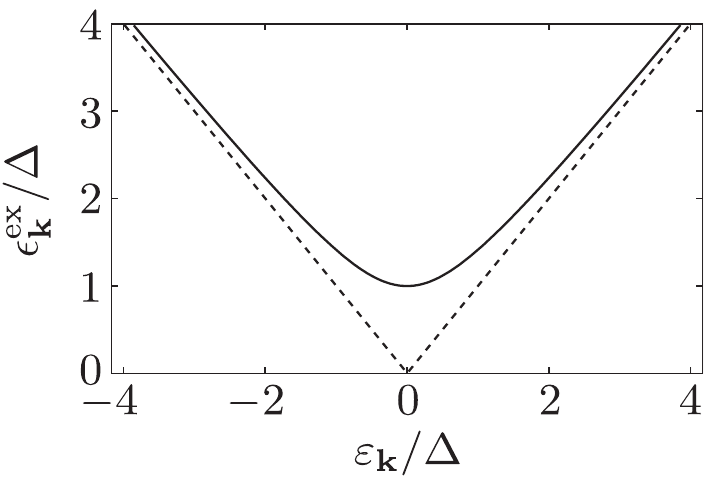
\includegraphics[width=0.5\textwidth]{immagini/Energia_eccitazione.png}
\end{figure}
\hspace{-0.6cm}Come possiamo vedere, se $\Delta=0$ si avrebbe una dispersione lineare. Se invece è presente l'interazione e quindi la superconduttività, l'energia delle eccitazioni è vicina a quella degli elettroni liberi quando $\xi_{\vb{k}} \gg \Delta$. Tuttavia, nella regione in cui $\xi_{\vb{k}} \ll \Delta$, cioè vicino allo zero dell'asse delle ascisse, il comportamento diventa completamente diverso: l'andamento è quadratico e, soprattutto, l'energia non si annulla mai. Esiste infatti un'energia minima necessaria per creare un'eccitazione, ed essa è proprio il gap energetico.\\
Più precisamente, se vogliamo rompere una coppia di Cooper, dobbiamo creare due stati eccitati, perché i due elettroni non vengono distrutti ma semplicemente trasformati in nuovi stati. Per questo motivo, quando parliamo di rottura di una coppia di Cooper, il costo energetico non è $\Delta$, bensì $2\Delta$, poiché è necessario separare entrambi gli elettroni della coppia.\\
Possiamo anche osservare come si comportino tutte le energie eccitate in funzione di $\vb{k}$:
\begin{figure}[H]
   \centering
   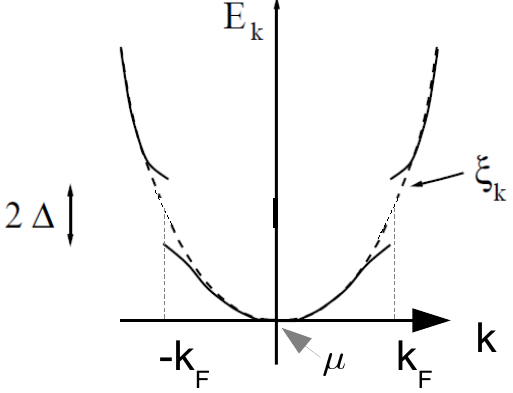
\includegraphics[width=0.5\textwidth]{immagini/Energia_eccitazione_rispetto_a_k.png}
\end{figure}
\hspace{-0.6cm}La linea tratteggiata rappresenta l'energia degli elettroni liberi, cioè l'energia degli elettroni in assenza di interazione:
\begin{equation*}
   E_{\vb{k}}
   =
   |\xi_{\vb{k}}|
   =
   \qty|
   \frac{\hbar^2 k^2}{2m}
   -
   \mu
   |
\end{equation*}
La linea continua rappresenta invece l'energia delle eccitazioni nello stato superconduttivo:
\begin{equation*}
   E_{\vb{k}}
   =
   \sqrt{
      \xi_{\vb{k}}^2
      +
      |\Delta|^2
   }
\end{equation*}
Osserviamo che in prossimità del vettore d'onda di Fermi compare un gap pari a $2\Delta$, perché gli elettroni che partecipano principalmente alla superconduttività sono proprio quelli vicini al livello di Fermi.\\
Abbiamo parlato di box di Nambu indipendenti; ciò significa che questi processi di eccitazione avvengono indipendentemente nei diversi box di Nambu. In questo senso possiamo interpretare tali eccitazioni come quasiparticelle non interagenti: ciascuna quasiparticella associata a un determinato box di Nambu non è direttamente collegata alle altre. Possiamo quindi usare il linguaggio delle quasiparticelle indipendenti nel senso che le eccitazioni presenti nei singoli box di Nambu risultano indipendenti tra loro.
\subsection{Condizione di autoconsistenza e gap energetico dipendente dalla temperatura}
Se vogliamo descrivere le proprietà che emergono da queste eccitazioni, cioè valutare le proprietà termodinamiche del sistema, dobbiamo considerare il fatto che tale sistema, nel quale sono presenti eccitazioni, si trova a temperatura finita. Il motivo per cui stiamo introducendo le eccitazioni è infatti capire cosa accade in un superconduttore a temperatura finita. Questo significa che dobbiamo determinare quale sia lo stato del sistema quando è presente una popolazione termica delle eccitazioni.\\
In generale, ciò viene descritto introducendo una matrice densità, esattamente nello stesso modo in cui si descrive un gas di Fermi normale a temperatura finita. Nel caso di un gas di Fermi normale, diciamo che le eccitazioni hanno energia $\varepsilon_{\vb{k}}$, e che il corrispondente stato è popolato con una probabilità legata all'occupazione termica; l'occupazione media è quindi espressa tramite la funzione di Fermi. Se vogliamo descrivere lo stato di tali particelle, dobbiamo considerare lo stato antisimmetrico rispetto allo scambio delle eccitazioni in equilibrio termico.\\
Qui dobbiamo fare esattamente la stessa cosa per queste quasiparticelle, poiché abbiamo visto che esse si comportano come gradi di libertà fermionici indipendenti in ciascun sottospazio. Se quindi vogliamo scrivere lo stato termico di queste particelle, dobbiamo introdurre una matrice densità della forma
\begin{equation*}
   W(T)
   =
   \frac{
      e^{-(H_{\rm MF}-\mu N_{\rm op})/k_B T}
   }{
      Z_{\rm MF}
   }
\end{equation*}
dove $Z_{\rm MF}$ è la funzione di partizione del sistema.\\
La probabilità di avere un'eccitazione è semplicemente data dalla funzione di Fermi, esattamente come nel caso di un normale gas di Fermi:
\begin{equation*}
   f(E^{\rm exc}_{\vb{k}})
   =
   \qty[
      1+
      e^{E^{\rm exc}_{\vb{k}}/k_B T}
   ]^{-1}
\end{equation*}
Quando abbiamo derivato lo stato fondamentale BCS, abbiamo ottenuto una condizione di autoconsistenza per $\Delta$ dalla quale abbiamo ricavato il modo in cui $\Delta$, cioè il gap a temperatura nulla, dipende dall'intensità dell'interazione. Quella era una condizione di autoconsistenza in cui il valor medio era calcolato rispetto allo stato fondamentale BCS.\\
Adesso abbiamo una nuova condizione di autoconsistenza. Essa emerge matematicamente dal sistema di equazioni lineari che abbiamo appena derivato per esprimere l'energia delle eccitazioni. Si tratta sostanzialmente dello stesso tipo di condizione di autoconsistenza; l'unica differenza è che ora i valori medi sui due membri dell'equazione vengono valutati rispetto allo stato di equilibrio termico che tiene conto delle eccitazioni.\\
Questo significa che il valor medio di $Z$ non è altro che il valor medio della combinazione di operatori che lo definisce. Poiché $Z$ è una combinazione di due operatori di creazione, dobbiamo esprimere tali operatori in termini dei nuovi operatori fermionici e poi valutare il valor medio di questa combinazione nello stato di equilibrio termico. Scriviamo quindi
\begin{equation*}
   \Delta(T)
   =
   V
   \sum_{\vb{k}}
   u^*_{\vb{k}}
   \nu_{\vb{k}}
   \expval*{Z_{\vb{k}}}
\end{equation*}
ossia\mn{Quello che stiamo facendo implicitamente è sostituire $Z_{\vb{k}}$ con la sua espressione in termini degli operatori di creazione e annichilazione, e poi esprimere questi ultimi in termini dei nuovi operatori fermionici $b$ invertendo la trasformazione di Bogoliubov--Valatin, trascurando i termini del tipo $b b$ e $b^\dag b^\dag$.}
\begin{equation*}
   \Delta(T) = V \sum_{\vb{k}} u^*_{\vb{k}} \nu_{\vb{k}} \expval*{ \bigl(1 - b^{\dag}_{\vb{k},\uparrow} b^{\vphantom{\dag}}_{\vb{k},\uparrow} -  b^{\dag}_{-\vb{k},\downarrow} b^{\vphantom{\dag}}_{-\vb{k},\downarrow} \bigr) }
\end{equation*}
I valori medi di queste combinazioni di operatori, $\expval*{b^{\dag}_{\vb{k},\uparrow} b^{\vphantom{\dag}}_{\vb{k},\uparrow}}$ e $\expval*{b^{\dag}_{-\vb{k},\downarrow} b^{\vphantom{\dag}}_{-\vb{k},\downarrow}}$, sono legati alla probabilità di trovare l'eccitazione rispettivamente negli stati $(\vb{k},\uparrow)$ e $(-\vb{k},\downarrow)$. Poiché tali quasiparticelle obbediscono alla statistica di Fermi-Dirac, si ha 
\begin{equation*}
   \expval*{b^{\dag}_{\vb{k},\uparrow} b^{\vphantom{\dag}}_{\vb{k},\uparrow}}
   =\expval*{b^{\dag}_{-\vb{k},\downarrow} b^{\vphantom{\dag}}_{-\vb{k},\downarrow}}
   =f(E_{\vb{k}})
\end{equation*}
Pertanto, la condizione di autoconsistenza per $\Delta$ assume la forma
\begin{equation*}
   \Delta(T)
   = V \sum_{\vb{k}} u^*_{\vb{k}} \nu_{\vb{k}} \bigl[ 1 - 2f(E_{\vb{k}}) \bigr]
   = V \sum_{\vb{k}} u^*_{\vb{k}} \nu_{\vb{k}} \tanh \qty( \frac{\beta E^{\rm exc}_{\vb{k}}}{2} )
\end{equation*}
Se adesso utilizziamo la relazione
\begin{equation*}
   u^*_{\vb{k}}
   \nu_{\vb{k}}
   =
   \frac{1}{2}
   \frac{
      \Delta
   }{
      \sqrt{
         \xi^2_{\vb{k}}
         +
         |\Delta|^2
      }
   }
\end{equation*}
la condizione di autoconsistenza per $\Delta$ assume la forma
\begin{equation*}
   \Delta(T)
   =
   \frac{|V|}{2}
   \sum_{\vb{k}}
   \frac{
      \Delta(T)
   }{
      \sqrt{
         \xi^2_{\vb{k}}
         +
         |\Delta|^2
      }
   }
   \tanh \qty[
      \frac{
         \beta
         \sqrt{
            \xi^2_{\vb{k}}
            +
            \Delta(T)^2
         }
      }{2}
   ]
\end{equation*}
Questa equazione è sostanzialmente la stessa ottenuta nel caso a temperatura nulla, tranne per il contributo aggiuntivo dipendente dalla temperatura.\\
Anche in questo caso la condizione può essere espressa come un integrale sull'energia, passando al limite del continuo e introducendo la densità degli stati:
\begin{equation*}
   1
   =
   \frac{|V|N(0)}{2}
   \int
   \dd{\xi}
   \frac{
      \tanh \qty(
         \beta
         \sqrt{
            \xi^2+\Delta(T)^2
         }/2
      )
   }{
      \sqrt{
         \xi^2+|\Delta|^2
      }
   }
\end{equation*}
A temperatura nulla otteniamo ciò che avevamo già trovato:
\begin{equation*}
   \Delta(0)
   =
   2\hbar\omega_D
   e^{-1/|V|N(0)}
\end{equation*}
mentre alla temperatura critica accade che $\Delta(T)\to0$. In questo caso, $E_{\vb{k}} \to |\xi_{\vb{k}}|$ e lo spettro delle eccitazioni diventa uguale a quello dello stato normale. Di conseguenza, $T_c$ si ottiene sostituendo $E_{\vb{k}}$ con $|\xi_{\vb{k}}|$ nell'equazione precedente:
\begin{equation}
   \frac{1}{|V|}
   =
   \frac{N(0)}{2}
   \int_{-\hbar\omega_D}^{\hbar\omega_D}
   \dd{\xi}
   \,
   \tanh\qty(
      \frac{\xi}{2k_B T_c}
   )
   \frac{1}{\xi}
   \label{eq:critical_temperature_integral}
\end{equation}
Questo integrale può essere risolto analiticamente. In particolare si può mostrare che
\begin{equation*}
   \frac{1}{|V|}
   =
   N(0)
   \ln\qty(
      2e^{\gamma}
      \frac{
         \hbar\omega_D
      }{
         \pi k_B T_c
      }
   )
\end{equation*}
e ciò permette di collegare la temperatura critica ai parametri che caratterizzano il superconduttore, in particolare l'intensità dell'interazione, la densità degli stati e l'energia di Debye. Invertendo questa relazione otteniamo
\begin{equation*}
   k_B T_c
   =
   \frac{
      2e^{\gamma}
   }{
      \pi
   }
   \hbar\omega_D
   e^{-1/N(0)|V|}
\end{equation*}
Possiamo ora confrontare il gap energetico a temperatura nulla con l'espressione della temperatura critica. Confrontando le due formule si trova infatti una relazione diretta tra queste quantità:
\begin{equation*}
   \Delta(0)
   \sim
   \frac{2}{A}
   k_B T_c
   \sim
   1.764\,k_B T_c
\end{equation*}
Il coefficiente numerico dipende dalle proprietà del materiale, ma per la maggior parte dei superconduttori di tipo I assume proprio questo valore.\\
Vediamo ora l'andamento del gap in funzione della temperatura. La quantità $\Delta(T)$ può essere calcolata numericamente a partire dall'\eqrefcustom{eq:critical_temperature_integral}. Per i superconduttori in regime di accoppiamento debole, nei quali $\hbar\omega_c/k_B T_c \gg 1$, il rapporto $\Delta(T)/\Delta(0)$ è una funzione universale di $T/T_c$ che decresce monotonicamente da $1$ a $T=0$ fino a $0$ a $T=T_c$, come mostrato nella figura seguente:
\begin{figure}[H]
   \centering
   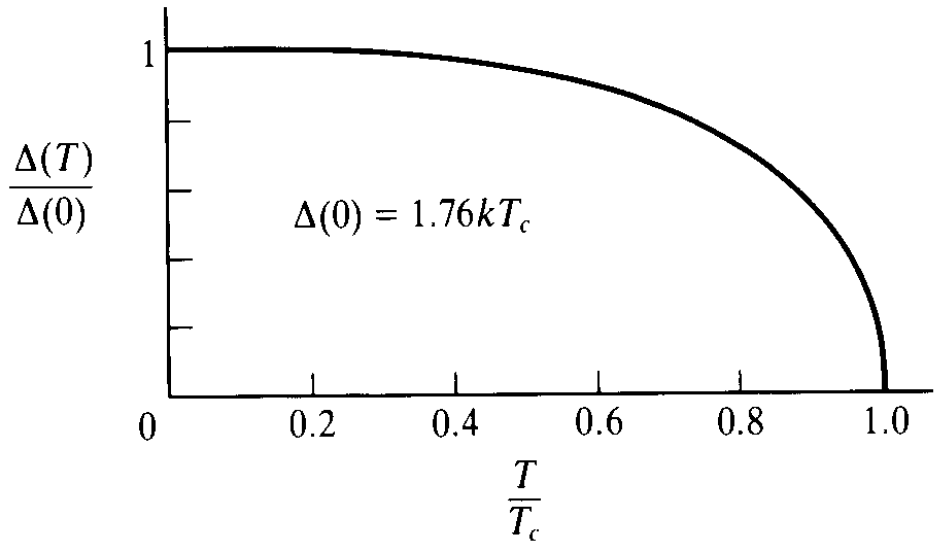
\includegraphics[width=0.6\textwidth]{immagini/Gap_temperature_dependence.png}
\end{figure}
\hspace{-0.6cm}Vicino a $T=0$, la variazione con la temperatura è esponenzialmente lenta, poiché $e^{-\Delta/k_B T} \approx 0$, così che la tangente iperbolica è praticamente uguale a $1$ e quasi indipendente dalla temperatura. Dal punto di vista fisico, ciò significa che $\Delta$ rimane quasi costante finché un numero significativo di quasiparticelle non viene eccitato termicamente.\\
Al contrario, per $T\simeq T_c$, il gap $\Delta(T)$ si annulla con tangente verticale, approssimativamente secondo la legge
\begin{equation*}
   \frac{\Delta(T)}{\Delta(0)}
   \approx 1.74 \qty( 1-\frac{T}{T_c} )^{1/2}
\end{equation*}
La dipendenza del parametro d'ordine $\Delta$ dalla radice quadrata di $(T_c-T)$ è una caratteristica generale di tutte le teorie di campo medio.
\subsection{Quantità termodinamiche}
Passiamo adesso alle proprietà termodinamiche. Abbiamo ormai tutti gli ingredienti necessari, poiché conosciamo $\Delta$, che dipende dalla temperatura.\\
Prima di procedere facciamo un passo indietro. Quando in meccanica quantistica abbiamo un'Hamiltoniana e la diagonalizziamo, otteniamo gli autostati e le autenergie $E_n$, che dipendono soltanto dai parametri dell'Hamiltoniana. Sappiamo poi che, a temperatura finita, la probabilità di trovare, ad esempio nel caso di una singola particella, il sistema in un autostato di energia $E_n$ è legata a $e^{-\beta E_n}$ nella combinazione appropriata, a seconda che le particelle siano fermioniche oppure bosoniche. Il punto importante è quindi che le autenergie dipendono soltanto dai parametri dell'Hamiltoniana.\\
Qui però abbiamo qualcosa di più sottile. Infatti, è vero che nel box di Nambu $\vb{k}$ abbiamo ottenuto delle energie $E_{\vb{k}}$ che dipendono da $\xi_{\vb{k}}$ e da $\Delta$, cioè da quantità legate ai parametri originari dell'Hamiltoniana; tuttavia, quando abbiamo imposto la condizione di autoconsistenza, abbiamo ottenuto un $\Delta$ dipendente dalla temperatura. Questo significa che ora le energie di eccitazione dipendono anch'esse dalla temperatura.\\
Il motivo per cui stiamo considerando energie di eccitazione dipendenti dalla temperatura è che dobbiamo includere questo parametro $\Delta(T)$, il quale dipende dalla temperatura proprio perché deve soddisfare la condizione di autoconsistenza derivante dall'approssimazione di campo medio introdotta in precedenza.\\
Le proprietà termodinamiche che vogliamo descrivere includono quindi un gap dipendente dalla temperatura direttamente nelle autenergie. Esse derivano essenzialmente dal considerare un gas di quasiparticelle fermioniche con numeri di occupazione dati dalla funzione di Fermi:
\begin{equation*}
   f_{\vb{k}}
   =\bigl[ 1+e^{\beta E_{\vb{k}}} \bigr]^{-1}
   \qq{dove}
   E_{\vb{k}}
   =
   \sqrt{ \xi_{\vb{k}}^2 + |\Delta(T)|^2 }
\end{equation*}
La peculiarità è che la temperatura non compare soltanto in $\beta$, ma entra anche direttamente nell'energia attraverso $\Delta(T)$.\\
Una volta compreso come trattare queste eccitazioni, possiamo utilizzare le usuali relazioni termodinamiche valide per un gas fermionico, espresse in termini dei numeri di occupazione. L'unica differenza è che tali numeri di occupazione dipendono dalle energie di eccitazione che abbiamo derivato, e che determinano a loro volta l'entropia elettronica nel modo usuale per un gas fermionico:
\begin{equation}
   S_{es}=-2k_B \sum_{\vb{k}} \Big[ (1-f_{\vb{k}}) \ln(1-f_{\vb{k}}) + f_{\vb{k}} \ln f_{\vb{k}} \Big]
   \label{eq:entropy}
\end{equation}
Una volta nota $S_{es}(T)$, il calore specifico può essere scritto come
\begin{equation}
   C_{es}
   =
   T\dv{S_{es}}{T}
   =
   -\beta\dv{S_{es}}{\beta}
   \label{eq:specific_heat_def}
\end{equation}
Usando l'\eqrefcustom{eq:entropy}, otteniamo
\begin{equation}
   \begin{split}
      C_{es}
      &= 2\beta k_B \sum_{\vb{k}} \pdv{f_{\vb{k}}}{\beta} \ln\qty( \frac{f_{\vb{k}}}{1 - f_{\vb{k}}} )\\
      &= -2\beta^2 k_B \sum_{\vb{k}} E_{\vb{k}} \pdv{f_{\vb{k}}}{\beta}
      \\
      &=
      -2\beta^2 k_B
      \sum_{\vb{k}}
      E_{\vb{k}}
      \frac{
         df_{\vb{k}}
      }{
         d(\beta E_{\vb{k}})
      }
      \qty(
         E_{\vb{k}}
         +
         \beta
         \frac{dE_{\vb{k}}}{d\beta}
      )
      \\
      &=
      2\beta k_B
      \sum_{\vb{k}}
      \frac{\partial f_{\vb{k}}}{\partial E_{\vb{k}}}
      \qty(
         E_{\vb{k}}^2
         +
         \frac{1}{2}
         \beta
         \frac{d\Delta^2}{d\beta}
      )
   \end{split}
   \label{eq:specific_heat_final}
\end{equation}
Il primo termine è quello usuale e deriva dalla ridistribuzione delle quasiparticelle tra i vari livelli energetici al variare della temperatura. Il secondo termine è invece più particolare e descrive l'effetto della dipendenza del gap dalla temperatura nel modificare direttamente i livelli energetici stessi.\\
Consideriamo ora questa espressione in due limiti. Il primo è il caso molto vicino alla temperatura critica $T_c$, dove $\Delta(T)\to0$ ed $E_{\vb{k}}$ si riduce a $\xi_{\vb{k}}$. In questo limite, il primo termine coincide con il normale calore specifico elettronico dello stato normale, $C_{en}=\gamma T$, che è continuo in $T_c$.\\
Il secondo termine invece è finito al di sotto di $T_c$, dove $\dv*{\Delta^2}{T}$ è grande, mentre è nullo al di sopra di $T_c$. Questo dà origine a una discontinuità $\Delta C$ nel calore specifico elettronico in corrispondenza di $T_c$. Si tratta del risultato che avevamo già introdotto all'inizio, ma che ora comprendiamo a partire dalla derivazione delle energie di eccitazione e della condizione di autoconsistenza, che introduce una dipendenza dalla temperatura anche nelle energie stesse.\\
Si può mostrare che l'ampiezza della discontinuità è
\begin{equation*}
   \Delta C
   =
   9.4\,N(0)k_B^2T_c
\end{equation*}
L'andamento complessivo del calore specifico elettronico è illustrato nella figura seguente:
\begin{figure}[H]
   \centering
   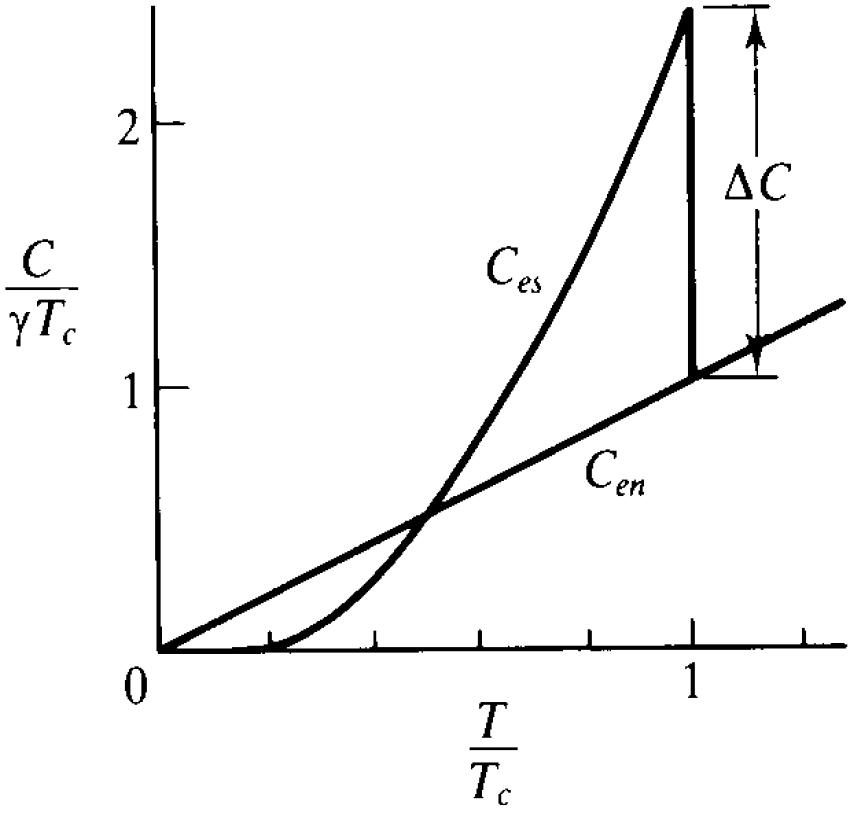
\includegraphics[width=0.5\textwidth]{immagini/Specific_heat.png}
\end{figure}
\hspace{-0.6cm}Consideriamo adesso il limite di temperature molto basse. In questo caso possiamo approssimare la funzione di Fermi con un comportamento esponenziale:
\begin{equation*}
   f_{\vb{k}}
   \approx
   e^{-E_{\vb{k}}/k_B T}
\end{equation*}
Abbiamo già osservato che a basse temperature è sempre presente un gap nello spettro, quindi possiamo descrivere le proprietà a bassa temperatura considerando il valore minimo del gap energetico, cioè $\Delta$. Inoltre abbiamo già visto che questo gap è proporzionale alla temperatura critica, quindi:
\begin{equation*}
   f_{\vb{k}}
   \approx
   e^{-\Delta/k_B T}
   =
   e^{-bT_c/T}
\end{equation*}
È evidente che, nel limite $T\ll T_c$, entrambi i termini in $C_{es}$ risultano esponenzialmente piccoli, poiché l'energia minima di eccitazione $\Delta$ è molto maggiore di $k_B T$. Questo spiega il comportamento esponenziale del calore specifico a basse temperature in un superconduttore:
\begin{equation*}
   C_{es}
   =
   \gamma T_c
   a
   e^{-bT_c/T}
\end{equation*}
Il fatto che il calore specifico sia non solo più piccolo, ma addirittura inferiore rispetto a quello di un metallo normale, deriva proprio dal comportamento della funzione di Fermi a basse temperature in presenza di un gap nello spettro. Più precisamente, tale andamento esponenziale discende direttamente dal comportamento esponenziale della funzione di Fermi.\\
Questi due regimi limite, temperatura nulla e temperatura critica, possono quindi essere compresi considerando la dipendenza delle autenergie dal gap superconduttivo e, più in generale, dalla temperatura.\\
Possiamo infine considerare anche le altre proprietà termodinamiche elettroniche, in particolare l'entropia, l'energia interna e l'energia libera di Helmholtz:
\begin{equation*}
   \begin{split}
      C_{el}
      & = T\dv{S_{es}}{T}
      = -\beta\dv{S_{es}}{\beta}
      \\
      F_{es}(T)
      & = U_{es}(T) - TS_{es}(T)
   \end{split}
\end{equation*}
\begin{figure}[H]
   \centering
   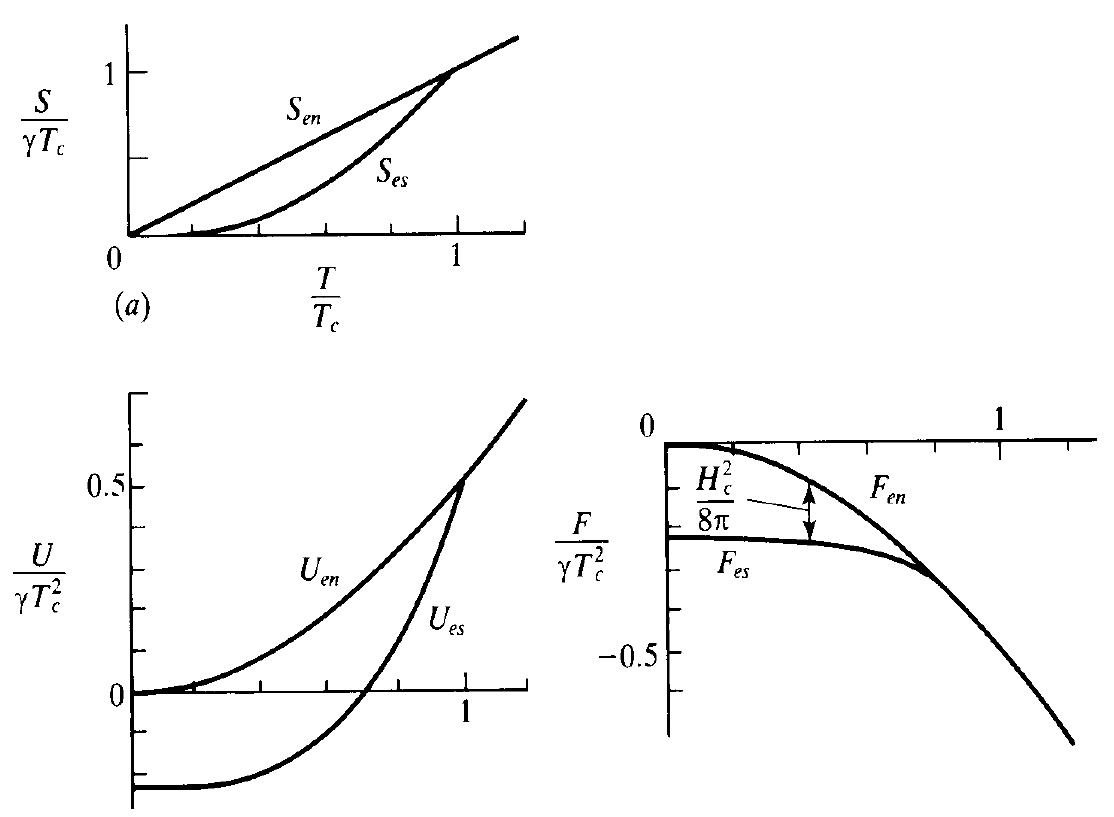
\includegraphics[width=0.9\textwidth]{immagini/Other_thermodynamic_quantities.png}
\end{figure}
\hspace{-0.6cm}Questi andamenti emergono immediatamente osservando la dipendenza dalla temperatura di tali quantità attraverso le energie di eccitazione. In particolare, in tutti questi casi non compare alcuna discontinuità, il che spiega perché la transizione superconduttiva a temperatura finita sia una transizione di fase del secondo ordine. Anche questo risultato emerge naturalmente dalla derivazione microscopica.
\subsection{Energie di eccitazione e densità degli stati}
Abbiamo visto che le energie di eccitazione assumono la forma
\begin{equation*}
   E_{\vb{k}}
   =
   \sqrt{
      \xi_{\vb{k}}^2
      +
      |\Delta|^2
   }
\end{equation*}
e che, per piccoli valori di $\xi_{\vb{k}}$, la dipendenza dall'energia è quadratica. Inoltre, per $\xi_{\vb{k}}=0$ compare un intervallo energetico nel quale le eccitazioni non possono esistere, cioè il gap che abbiamo già introdotto.\\
Abbiamo anche visto che tali eccitazioni vengono create e distrutte dagli operatori fermionici $b_{\vb{k},\uparrow}$ e $b^{\dag}_{\vb{k},\uparrow}$, che sono in corrispondenza biunivoca con gli operatori di creazione e distruzione degli elettroni ordinari $c_{\vb{k},\uparrow}$ e $c^{\dag}_{\vb{k},\uparrow}$, nel senso che sono legati a essi tramite trasformazioni lineari.\\
Questa corrispondenza implica che, se vogliamo valutare la densità degli stati di queste eccitazioni, possiamo assumere che esse abbiano una densità $N_s(E)$ tale che il numero di eccitazioni comprese nell'intervallo energetico $\dd{E}$, cioè $N_s(E)\dd{E}$, corrisponda esattamente al numero di stati elettronici normali con energia compresa nell'intervallo $\dd{\xi}$. In altre parole, dobbiamo uguagliare il numero di stati del superconduttore al numero di stati del metallo normale:
\begin{equation*}
   N_s(E)\dd{E}=N_n(\xi)\dd{\xi}
\end{equation*}
Questi numeri coincidono proprio grazie alla corrispondenza tra gli operatori fermionici dei due problemi.\\
Questa identità permette di ricavare molto facilmente la densità degli stati del superconduttore. Infatti possiamo riscriverla come
\begin{equation*}
   \frac{ N_s(E) }{
      N_n(\xi)
   }
   =
   \dv{\xi}{E}
\end{equation*}
Poiché siamo interessati principalmente a energie $\xi$ che differiscono dal livello di Fermi solo di pochi meV, possiamo approssimare la densità degli stati normale come costante:
\begin{equation*}
   N_n(\xi)\approx N(0)
\end{equation*}
Inoltre, dato che conosciamo esplicitamente la dipendenza di $\xi$ da $E$, possiamo calcolare la derivata e ottenere
\begin{equation*}
   \frac{ N_s(E)}{N_n(\xi)}
   =
   \begin{dcases}
      \frac{E}{\sqrt{ E^2 -|\Delta|^2}}
      & \text{per } E>\Delta
      \\[0.3cm]
      0
      & \text{per } E<\Delta
   \end{dcases}
\end{equation*}
La densità degli stati delle eccitazioni si annulla quindi per energie inferiori al gap, come è naturale aspettarsi dato che abbiamo visto che in quella regione non esistono eccitazioni. Per energie superiori a $\Delta$, invece, la densità degli stati deriva semplicemente dalla derivata di $\xi$ rispetto a $E$.\\
Possiamo rappresentare graficamente questa densità degli stati:
\begin{figure}[H]
   \centering
   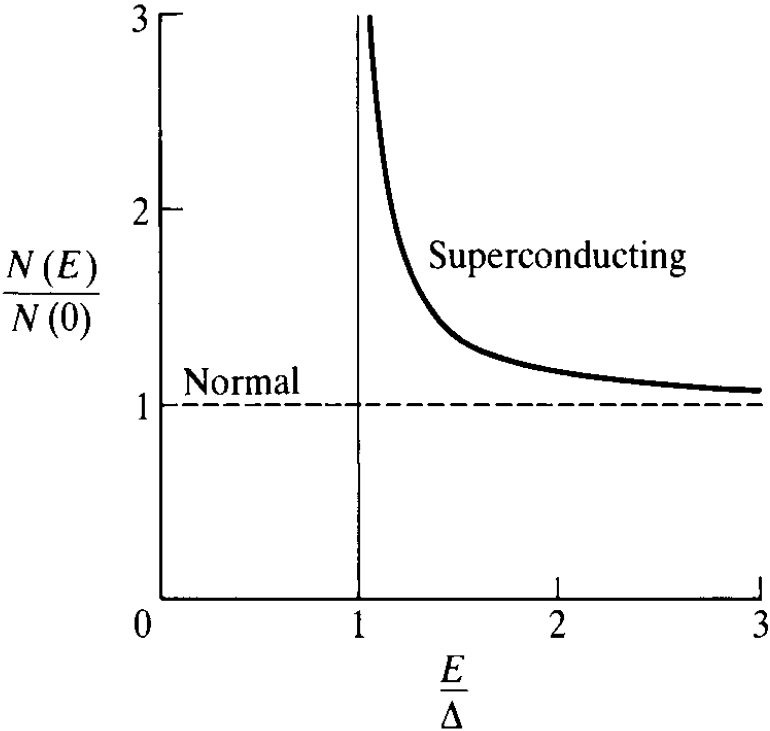
\includegraphics[width=0.5\textwidth]{immagini/Density_of_states.png}
\end{figure}
\hspace{-0.6cm}Come si vede, la densità degli stati è nulla per energie inferiori al gap, cioè per $E/\Delta<1$. Per energie molto maggiori di $\Delta$, essa tende invece al valore del metallo normale. Infatti, nel limite $E\gg\Delta$, si ha
\begin{equation*}
   \frac{
      E
   }{
      \sqrt{
         E^2-|\Delta|^2
      }
   }
   \approx
   \frac{
      E
   }{
      \sqrt{E^2}
   }
   =
   1
\end{equation*}
Nel limite $E\to\Delta$, cioè quando $E/\Delta \to 1$, il denominatore tende a zero e compare quindi una divergenza della densità degli stati in prossimità del gap.\\
La densità degli stati di un superconduttore presenta quindi tre caratteristiche fondamentali:
\begin{itemize}[leftmargin=0.5cm]
   \item è nulla per energie inferiori al gap;
   \item tende alla densità degli stati del metallo normale per energie molto maggiori del gap;
   \item presenta una divergenza in corrispondenza del bordo del gap.
\end{itemize}
Quest'ultimo comportamento riflette il fatto che, vicino al gap, gli stati di eccitazione si accumulano fortemente.
\subsection{Elettrodinamica dei superconduttori BCS}
Vediamo ora quali siano le conseguenze di questa densità degli stati.\\
Consideriamo la risposta a un campo magnetico statico. Supponiamo quindi di avere un campo magnetico $\vb{B}$ generato da un potenziale vettore $\vb{A}$.\\
Quello che vogliamo capire è innanzitutto quale sia l'effetto della presenza di un campo magnetico sull'Hamiltoniana complessiva del sistema, dato che finora abbiamo considerato l'Hamiltoniana BCS in assenza di campo magnetico. Come facciamo? Dobbiamo considerare il modo in cui il campo magnetico influenza il sistema elettronico.\\
Sappiamo che, in generale, per particelle con momento $\vb{p}$ e carica $e$, il momento viene sostituito con il momento gauge-invariante:
\begin{equation*}
   \vb{p}
   \to
   \vb{p}
   -
   \frac{e}{c}\vb{A}
\end{equation*}
Questo significa che il termine cinetico dell'Hamiltoniana viene modificato nel modo seguente:
\begin{equation*}
   \frac{\vb{p}^2}{2m}
   \to
   \frac{1}{2m}
   \qty(
      \vb{p}
      -
      \frac{e}{c}\vb{A}
   )^2
\end{equation*}
ossia
\begin{equation*}
   \frac{1}{2m}
   \qty(
      \vb{p}
      -
      \frac{e}{c}\vb{A}
   )^2
   =
   \frac{1}{2m}
   \qty(
      \vb{p}^2
      +
      \frac{e^2}{c^2}\vb{A}^2
      -
      \frac{e}{c}\vb{p}\vdot\vb{A}
      -
      \frac{e}{c}\vb{A}\vdot\vb{p}
   )
\end{equation*}
Poiché siamo interessati soltanto alla risposta lineare a campi deboli, manteniamo solo i termini lineari in $\vb{A}$ e trascuriamo quindi il termine proporzionale a $\vb{A}^2$.\\
Esprimendo l'operatore $\vb{p}$ come $-i\hbar\grad$,il termine cinetico diventa
\begin{equation*}
   \frac{1}{2m}
   \qty(
      \vb{p}
      -
      \frac{e}{c}\vb{A}
   )^2
   =
   \frac{\vb{p}^2}{2m}
   +
   i\hbar\frac{e}{2mc}\div{\vb{A}}
   +
   i\hbar\frac{e}{2mc}\vb{A}\vdot\grad
\end{equation*}
Se scegliamo la gauge di London, per cui
\[
\div{\vb{A}}=0,
\]
il secondo termine si annulla e rimane\mn{Sono abbastanza convinto che questa parte sia sbagliata e che in realtà i due termini si possano sommare.}
\begin{equation*}
   \frac{1}{2m}
   \qty(
      \vb{p}
      -
      \frac{e}{c}\vb{A}
   )^2
   =
   \frac{\vb{p}^2}{2m}
   +
   i\frac{e\hbar}{mc}\vb{A}\vdot\grad
\end{equation*}
Il passo successivo consiste nel capire come questo termine perturbativo possa essere scritto in seconda quantizzazione, cioè esplicitamente in termini di operatori di creazione e distruzione elettronici.\\
Per farlo dobbiamo vedere come tale termine agisce sulle onde piane corrispondenti a uno stato con momento $\vb{k}$. Abbiamo
\begin{equation*}
   \vb{A}\vdot\grad
   e^{i\vb{k}\vdot\vb{r}}
   =
   i\vb{A}\vdot\vb{k}
   e^{i\vb{k}\vdot\vb{r}}
\end{equation*}
Questo significa che, se vogliamo trovare la rappresentazione di questo termine di interazione nella base delle onde piane, dobbiamo utilizzare l'azione del gradiente sulle onde piane. Inoltre, conviene espandere il potenziale vettore in trasformata di Fourier:
\begin{equation*}
   \vb{A}(\vb{r})
   =
   \sum_{\vb{q}}
   \vb{a}(\vb{q})
   e^{i\vb{q}\vdot\vb{r}}
\end{equation*}
Il termine di interazione assume allora la forma
\begin{equation*}
   V
   =
   i\frac{e \hbar}{mc}
   \sum_{\vb{k}}
   \sum_{\vb{q}}
   \vb{a}(\vb{q})
   \vdot
   i\vb{k}
   e^{i(\vb{q}+\vb{k})\vdot\vb{r}}
\end{equation*}
Cerchiamo di capire il significato fisico di questa espressione. L'idea è che, se questo termine di interazione agisce su un'elettrone con momento $\vb{k}$, esso ne modifica il momento in $\vb{k}+\vb{q}$.\\
Questo significa che l'interazione descrive un processo di scattering in cui un elettrone con momento $\vb{k}$ viene trasformato in uno stato con momento $\vb{k}+\vb{q}$ senza modificarne lo spin.\\
Di conseguenza, l'operatore di seconda quantizzazione che descrive tale processo deve distruggere un elettrone con momento $\vb{k}$ e crearne uno con momento $\vb{k}+\vb{q}$. Si ottiene quindi
\begin{equation*}
   V
   =
   -
   \frac{e \hbar}{mc}
   \sum_{\vb{k}}
   \sum_{\vb{q}}
   \sum_{\sigma}
   \vb{a}(\vb{q})
   \vdot
   \vb{k}
   \,
   c^{\dag}_{\vb{k}+\vb{q},\sigma}
   c^{\vphantom{\dag}}_{\vb{k},\sigma}
\end{equation*}
Questa è quindi la forma del termine aggiuntivo che deve essere incluso nell'Hamiltoniana BCS quando si considera l'azione di un campo magnetico esterno.\\
A questo punto introduciamo un'approssimazione. Finora $\vb{a}(\vb{q})$ contiene tutti i possibili momenti, cioè stiamo considerando un potenziale vettore completamente generico. L'idea ora è quella di considerare il regime in cui il campo magnetico è quasi uniforme all'interno del superconduttore. Questo significa che anche le variazioni spaziali del potenziale vettore sono molto lente e quindi sono rilevanti soltanto valori piccoli di $\vb{q}$.\\
Possiamo quindi sostituire
\[
\vb{a}(\vb{q})
\to
\vb{a}(0),
\]
effettuando quella che viene chiamata \emph{approssimazione a grande lunghezza d'onda}. In questa approssimazione l'interazione si semplifica ulteriormente:
\begin{equation*}
   V
   \simeq
   -
   \frac{e \hbar}{mc}
   \sum_{\vb{k}}
   \sum_{\sigma}
   \vb{a}(0)\vdot\vb{k}
   \,
   c^{\dag}_{\vb{k},\sigma}
   c^{\vphantom{\dag}}_{\vb{k},\sigma}
\end{equation*}
Ricordiamo ora che gli operatori $c_{\vb{k},\sigma}$ sono legati agli operatori $b_{\vb{k},\uparrow}$ e $b_{-\vb{k},\downarrow}$ attraverso la trasformazione di Bogoliubov. Possiamo quindi riscrivere il termine di interazione in funzione degli operatori che creano e distruggono le eccitazioni del superconduttore. Invertendo l'\eqrefcustom{eq:Bogoliubov_Valatin_transformation_explicit}, si ottiene
\begin{equation*}
   V = - \frac{e \hbar}{2mc} \sum_{\vb{k}} \vb{a}(0)\vdot\vb{k} \qty[ b^{\dag}_{\vb{k},\uparrow} b^{\vphantom{\dag}}_{\vb{k},\uparrow} - b^{\dag}_{-\vb{k},\downarrow} b^{\vphantom{\dag}}_{-\vb{k},\downarrow} ]
\end{equation*}
L'Hamiltoniana BCS complessiva diventa quindi
\begin{equation*}
   H_{\rm BCS} = \sum_{\vb{k},\sigma} E_{\vb{k}} b^{\dag}_{\vb{k},\sigma} b^{\vphantom{\dag}}_{\vb{k},\sigma} - \frac{e \hbar}{2mc} \sum_{\vb{k}} \vb{a}(0)\vdot\vb{k} \qty[ b^{\dag}_{\vb{k},\uparrow} b^{\vphantom{\dag}}_{\vb{k},\uparrow} - b^{\dag}_{-\vb{k},\downarrow} b^{\vphantom{\dag}}_{-\vb{k},\downarrow} ]
\end{equation*}
Osserviamo che questa Hamiltoniana è ancora diagonale. Possiamo quindi scriverla come
\begin{equation*}
   H_{\rm BCS}
   =
   \sum_{\vb{k},\sigma}
   \tilde{E}_{\vb{k}}
   b^{\dag}_{\vb{k},\sigma}
   b^{\vphantom{\dag}}_{\vb{k},\sigma}
\end{equation*}
dove
\begin{equation*}
   \begin{split}
      \tilde{E}_{\vb{k},\uparrow}
      &=
      E_{\vb{k},\uparrow}
      -
      \frac{e\hbar}{mc}
      \vb{a}(0)\vdot\vb{k}
      =
      E_{\vb{k},\uparrow}
      -
      \delta
      \\[0.2cm]
      \tilde{E}_{-\vb{k},\downarrow}
      &=
      E_{-\vb{k},\downarrow}
      +
      \frac{e\hbar}{mc}
      \vb{a}(0)\vdot\vb{k}
      =
      E_{-\vb{k},\downarrow}
      +
      \delta
   \end{split}
\end{equation*}
Una volta scritta esplicitamente l'Hamiltoniana modificata, vogliamo determinare la risposta elettromagnetica del superconduttore, cioè la densità di corrente. L'obiettivo finale è ottenere una relazione tra la corrente e il potenziale vettore e recuperare eventualmente l'equazione di London con una forma esplicita della lunghezza di penetrazione.\\
Il punto di partenza è scrivere la densità di corrente:
\begin{equation*}
   \vb{J}
   =
   \frac{ne}{m}\vb{p}
   -
   \frac{ne^2}{mc}\vb{A}
   =
   \vb{J}_1+\vb{J}_2
\end{equation*}
Il termine $\vb{J}_1$ è detto termine paramagnetico, mentre $\vb{J}_2$ è il termine diamagnetico.\\
Scriviamo esplicitamente $\vb{J}_1$. Sostituendo
\[
\vb{p}\to -i\hbar\grad
\]
e considerando l'azione sulle onde piane:
\begin{equation*}
   \vb{p}
   e^{i\vb{k}\vdot\vb{r}}
   =
   -i\hbar
   \grad
   e^{i\vb{k}\vdot\vb{r}}
   =
   \hbar\vb{k}
   e^{i\vb{k}\vdot\vb{r}}
\end{equation*}
Otteniamo quindi
\begin{equation*}
   \vb{J}_1
   =
   \frac{ne\hbar}{m}
   \sum_{\vb{k},\sigma}
   \vb{k}
   c^{\dag}_{\vb{k},\sigma}
   c^{\vphantom{\dag}}_{\vb{k},\sigma}
\end{equation*}
ossia
\begin{equation*}
   \vb{J}_1
   =
   \frac{ne\hbar}{m}
   \sum_{\vb{k}}
   \vb{k}
   \qty[
      b^{\dag}_{\vb{k},\uparrow}
      b^{\vphantom{\dag}}_{\vb{k},\uparrow}
      -
      b^{\dag}_{\vb{k},\downarrow}
      b^{\vphantom{\dag}}_{\vb{k},\downarrow}
   ]
\end{equation*}
Per il termine diamagnetico utilizziamo invece lo sviluppo di Fourier del potenziale vettore:
\begin{equation*}
   \vb{J}_2
   =
   -
   \frac{ne^2}{mc}
   \sum_{\vb{q}}
   \vb{a}(\vb{q})
   e^{i\vb{q}\vdot\vb{r}}
\end{equation*}
Nell'approssimazione a grande lunghezza d'onda:
\begin{equation*}
   \vb{J}_2
   \simeq
   -
   \frac{ne^2}{mc}
   \vb{a}(0)
\end{equation*}
A questo punto vogliamo valutare il valor medio termico della corrente a temperatura finita ma inferiore a $T_c$. Iniziamo con $\expval*{\vb{J}_1}$:
\begin{equation*}
   \expval*{\vb{J}_1}
   =
   \frac{ne\hbar}{m}
   \sum_{\vb{k}}
   \vb{k}
   \qty[
      \expval*{
         b^{\dag}_{\vb{k},\uparrow}
         b^{\vphantom{\dag}}_{\vb{k},\uparrow}
      }
      -
      \expval*{
         b^{\dag}_{\vb{k},\downarrow}
         b^{\vphantom{\dag}}_{\vb{k},\downarrow}
      }
   ]
\end{equation*}
Questi valori medi non sono altro che le occupazioni termiche fermioniche delle quasiparticelle, quindi
\begin{equation*}
   \expval*{
      b^{\dag}_{\vb{k},\uparrow}
      b^{\vphantom{\dag}}_{\vb{k},\uparrow}
   }
   =
   f(\tilde{E}_{\vb{k},\uparrow})
\end{equation*}
e
\begin{equation*}
   \expval*{
      b^{\dag}_{\vb{k},\downarrow}
      b^{\vphantom{\dag}}_{\vb{k},\downarrow}
   }
   =
   f(\tilde{E}_{\vb{k},\downarrow})
\end{equation*}
Espandendo la funzione di Fermi al primo ordine in $\delta$:
\begin{equation*}
   \begin{split}
      f(\tilde{E}_{\vb{k},\uparrow})
      &\approx
      f(E_{\vb{k},\uparrow})
      -
      \delta
      \eval{\pdv{f}{E}}_{\delta=0}
      \\[0.2cm]
      f(\tilde{E}_{-\vb{k},\downarrow})
      &\approx
      f(E_{-\vb{k},\downarrow})
      +
      \delta
      \eval{\pdv{f}{E}}_{\delta=0}
   \end{split}
\end{equation*}
Nel limite di piccolo $\vb{a}(0)$:
\begin{equation*}
   f(E_{\vb{k},\uparrow})
   =
   f(E_{-\vb{k},\downarrow}),
\end{equation*}
per cui
\begin{equation*}
   f(\tilde{E}_{\vb{k},\uparrow})
   -
   f(\tilde{E}_{-\vb{k},\downarrow})
   =
   -2\delta
   \eval{\pdv{f}{E}}_{\delta=0}
\end{equation*}
Segue allora
\begin{equation*}
   \expval*{\vb{J}_1}
   =
   -2
   \frac{ne\hbar}{m}
   \sum_{\vb{k}}
   \vb{k}
   \,
   \delta
   \eval{\pdv{f}{E}}_{\delta=0}
\end{equation*}
Sostituendo esplicitamente $\delta$:
\begin{equation*}
   \expval*{\vb{J}_1}
   =
   -2
   \frac{n(e\hbar)^2}{m^2c}
   \sum_{\vb{k}}
   \eval{\pdv{f}{E}}_{\delta=0}
   \vb{k}
   \,
   \vb{a}(0)\vdot\vb{k}
\end{equation*}
Osserviamo che
\begin{equation*}
   \vb{a}(0)\vdot\vb{k}
   =
   a(0)k\cos\vartheta_k
\end{equation*}
dove $\vartheta_k$ è l'angolo tra $\vb{a}(0)$ e $\vb{k}$.\\
Poiché ci aspettiamo che la corrente media sia parallela a $\vb{a}(0)$, effettuiamo la sostituzione
\begin{equation*}
   \vb{k}
   \to
   k\cos\vartheta_k
   \frac{\vb{a}(0)}{a(0)}
\end{equation*}
Otteniamo quindi
\begin{equation*}
   \expval*{\vb{J}_1}
   =
   -2
   \frac{n(e\hbar)^2}{m^2c}
   \sum_{\vb{k}}
   \eval{\pdv{f}{E}}_{\delta=0}
   (k\cos\vartheta_k)^2
   \vb{a}(0)
\end{equation*}
Aggiungendo anche il contributo diamagnetico:
\begin{equation*}
   \expval*{\vb{J}}
   =
   -2
   \frac{n(e\hbar)^2}{m^2c}
   \sum_{\vb{k}}
   \eval{\pdv{f}{E}}_{\delta=0}
   (k\cos\vartheta_k)^2
   \vb{a}(0)
   -
   \frac{ne^2}{mc}
   \vb{a}(0)
\end{equation*}
Facendo la media angolare:
\begin{equation*}
   \expval*{
      (k\cos\vartheta_k)^2
   }
   =
   \frac13
   \expval*{k_F^2}
\end{equation*}
e usando
\begin{equation*}
   k_F^2
   =
   \frac{2mE_F}{\hbar^2},
\end{equation*}
si ottiene
\begin{equation*}
   \expval*{\vb{J}}
   =
   \frac{
      4ne^2E_F
   }{
      3mc
   }
   \sum_{\vb{k}}
   \qty(
      -
      \eval{\pdv{f}{E}}_{\delta=0}
   )
   \vb{a}(0)
   -
   \frac{ne^2}{mc}
   \vb{a}(0)
\end{equation*}
Sostituendo la somma con un integrale:
\begin{equation*}
   \expval*{\vb{J}}
   =
   \frac{
      4ne^2E_F
   }{
      3mc
   }
   \int_{-\infty}^{+\infty}
   \dd{\xi}
   N(\xi)
   \qty(
      -
      \eval{\pdv{f}{E}}_{\delta=0}
   )
   \vb{a}(0)
   -
   \frac{ne^2}{mc}
   \vb{a}(0)
\end{equation*}
Riconosciamo ora la stessa struttura della teoria di London:
\begin{equation*}
   \vb{J}
   =
   -
   \frac{c}{4\pi}
   \frac{\vb{A}}{\lambda^2(T)}
\end{equation*}
Definendo la lunghezza di penetrazione a temperatura nulla come\mn{La ragione per cui questa è la lunghezza di penetrazione a temperatura nulla è che a $T=0$ la derivata della funzione di Fermi è nulla.}
\begin{equation*}
   \frac{1}{\lambda^2(0)}
   =
   \frac{4\pi ne^2}{mc^2},
\end{equation*}
otteniamo infine
\begin{equation*}
   \frac{
      \lambda^2(0)
   }{
      \lambda^2(T)
   }
   =
   \frac{4E_F}{3}
   \int_{-\infty}^{+\infty}
   \dd{\xi}
   N(\xi)
   \eval{\pdv{f}{E}}_{\delta=0}
   +
   1
\end{equation*}
Possiamo rappresentare questo risultato in funzione di $T/T_c$:
\begin{figure}[H]
   \centering
   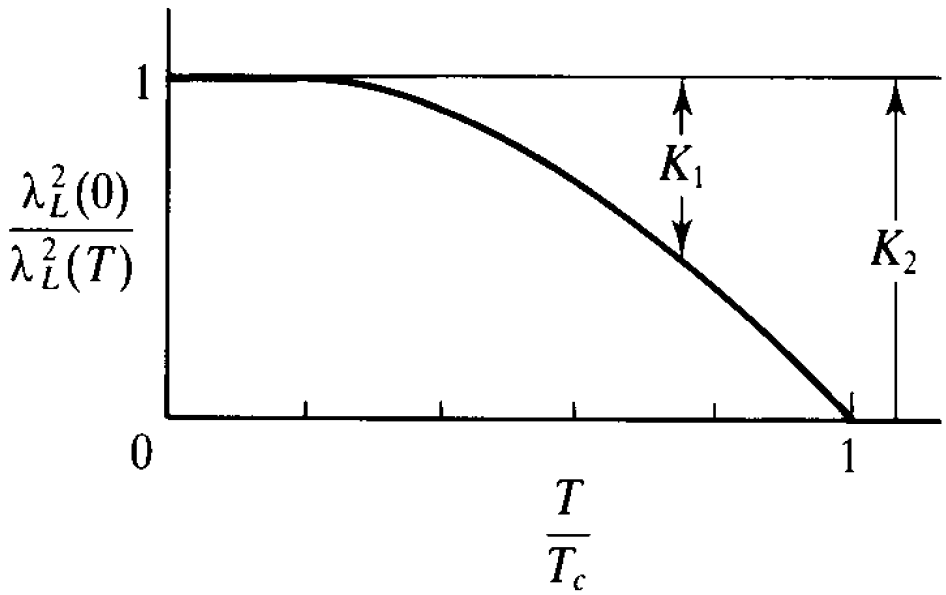
\includegraphics[width=0.5\textwidth]{immagini/Penetration_depth_BCS.png}
\end{figure}
\hspace{-0.6cm}A temperatura nulla il termine integrale si annulla e la lunghezza di penetrazione coincide con $\lambda(0)$. A temperatura finita, invece, la lunghezza di penetrazione aumenta e diverge quando ci si avvicina alla temperatura critica.\\
Possiamo inoltre valutare esplicitamente l'integrale usando la densità degli stati del superconduttore:
\begin{equation*}
   \begin{split}
      \frac{
         \lambda_L^2(0)
      }{
         \lambda_L^2(T)
      }
      &=
      1
      -
      \int_{-\infty}^{+\infty}
      \dd{\xi}
      \frac{
         N_s(E)
      }{
         N_s(0)
      }
      \qty(
         -
         \eval{\pdv{f}{E}}_{\delta=0}
      )
      \\[0.3cm]
      &=
      1
      -
      2
      \int_{\Delta}^{+\infty}
      \dd{E}
      \frac{
         E
      }{
         \sqrt{
            E^2-|\Delta|^2
         }
      }
      \qty(
         -
         \eval{\pdv{f}{E}}_{\delta=0}
      )
   \end{split}
\end{equation*}
Otteniamo così una forma esplicita della lunghezza di penetrazione in funzione della temperatura, espressa in termini della densità degli stati derivata dalle eccitazioni del superconduttore.\\
Questo mostra come sia possibile utilizzare la teoria microscopica BCS, e in particolare le eccitazioni rispetto allo stato fondamentale BCS, per derivare proprietà macroscopiche del superconduttore a temperatura finita, ottenendo una descrizione quantitativa della lunghezza di penetrazione e della risposta elettromagnetica del sistema.

\chapter{Dispositivi superconduttivi}
\section{Tunneling elettronico}
Cominciamo ora a vedere le conseguenze della struttura dei livelli energetici di un superconduttore, in particolare non solo della struttura dello stato fondamentale, ma anche delle eccitazioni. Considereremo i fenomeni di tunneling di singolo elettrone e successivamente parleremo dell'effetto Josephson. In entrambi i casi si tratta di fenomeni di trasporto, cioè situazioni in cui vi è una corrente che fluisce nel dispositivo.\\
Quello che dobbiamo tenere a mente è la densità degli stati delle eccitazioni. Le eccitazioni hanno una dipendenza dall'energia rispetto al livello di Fermi e dal gap energetico in funzione di $\xi_{\vb{k}}$; la dipendenza ha una forma parabolica, in contrasto con il comportamento lineare che si ha nel caso del gas di Fermi normale in assenza di superconduttività.\\
Vediamo inoltre che esiste una regione di energie proibite per le eccitazioni, cioè il gap energetico, e che il costo energetico necessario per creare un'eccitazione, ossia rompere una coppia di Cooper, è pari a $2\Delta$, poiché dobbiamo eccitare due elettroni.\\
Abbiamo detto che, poiché gli operatori di creazione e distruzione delle eccitazioni sono in corrispondenza biunivoca con gli operatori di creazione e distruzione delle particelle elettroniche, nel senso che tra di essi esiste una relazione lineare, la densità degli stati delle eccitazioni, $N_s(E)$, deve corrispondere al numero di stati disponibili nel metallo normale, $N_n(\xi)$.\\
Imponendo questa corrispondenza abbiamo ricavato la densità degli stati delle eccitazioni del superconduttore, che si annulla per energie minori del gap e presenta invece il comportamento caratteristico per energie maggiori di $\Delta$, con una divergenza in prossimità di $E=\Delta$.\\
Questa divergenza deriva dal fatto che nel superconduttore non esiste alcuna densità degli stati per energie inferiori al gap, mentre in un normale gas di Fermi la densità degli stati rimane praticamente uniforme a partire da energia nulla.\\
Vedremo ora che, se consideriamo delle giunzioni, cioè sistemi in cui uno o due superconduttori sono separati da uno strato isolante, eventualmente con un metallo normale dall'altro lato, la corrente che fluisce attraverso la giunzione dipende dalla densità degli stati. In opportune condizioni, la conduttanza differenziale risulta direttamente proporzionale alla densità degli stati.\\
Di conseguenza, misurando la corrente che attraversa la giunzione e valutando la conduttanza differenziale, è possibile ottenere informazioni dirette sulla densità degli stati delle eccitazioni del superconduttore.
\subsection{Giunzione Normale--Isolante--Normale (NIN)}
Il tunneling elettronico è il fenomeno di tunneling che conosciamo dalla meccanica quantistica standard, cioè la possibilità per una particella di attraversare una regione in cui non vi sarebbe conservazione dell'energia e che sarebbe quindi classicamente proibita. Questo fenomeno si verifica anche nel caso di metalli normali, in particolare quando consideriamo una giunzione normale--isolante--normale (NIN), in cui un sottile strato isolante di pochi nanometri separa due metalli normali. Se la giunzione è collegata a un generatore di tensione, attraverso il dispositivo può fluire una corrente, e ora vedremo come descrivere tale corrente.
\begin{figure}[H]
    \centering
    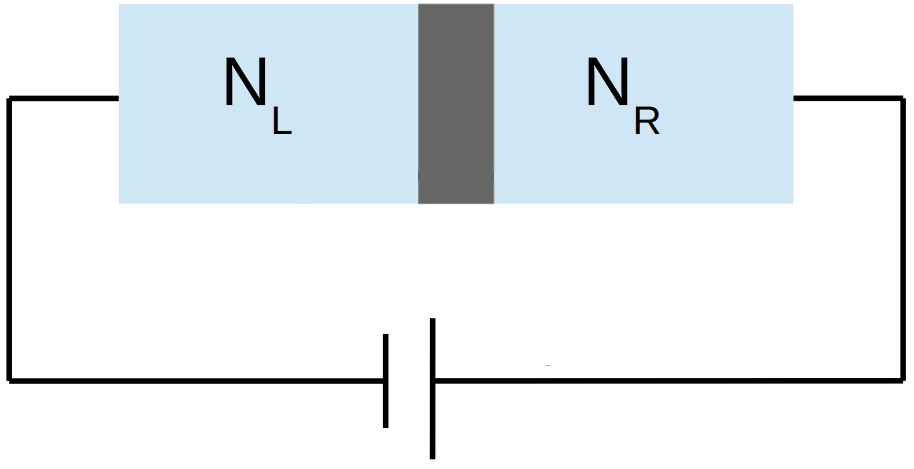
\includegraphics[width=0.5\textwidth]{immagini/NIN_junction.png}
\end{figure}
\hspace{-0.6cm}L'idea è che, a causa dell'effetto tunnel, esista una probabilità non nulla che un elettrone passi dal lead sinistro a quello destro o viceversa.\\
Come descriviamo quantisticamente questo processo? L'idea è partire dall'Hamiltoniana complessiva del sistema, che consiste nell'Hamiltoniana del lead sinistro, quella del lead destro e un termine di tunneling:
\begin{equation*}
    H=H_L + H_R + H_T
\end{equation*}
Poiché sia il lead sinistro che quello destro sono metalli normali, le rispettive Hamiltoniane sono semplicemente le Hamiltoniane in seconda quantizzazione che descrivono gli elettroni liberi in un metallo, con i consueti operatori di creazione e distruzione. Per distinguere i due lead utilizzeremo l'indice $\vb{k}$ per il lead sinistro e l'indice $\vb{q}$ per quello destro. Si ha quindi
\begin{equation*}
    H_L
    =
    \sum_{\vb{k}, \sigma}
    \varepsilon^{\vphantom{\dag}}_{\vb{k},\sigma}
    c^{\dag}_{\vb{k}, \sigma}
    c^{\vphantom{\dag}}_{\vb{k}, \sigma}
    \qq{,}
    H_R
    =
    \sum_{\vb{q}, \sigma}
    \varepsilon^{\vphantom{\dag}}_{\vb{q},\sigma}
    c^{\dag}_{\vb{q}, \sigma}
    c^{\vphantom{\dag}}_{\vb{q}, \sigma}
\end{equation*}
dove $\varepsilon_{\vb{k},\sigma}$ e $\varepsilon_{\vb{q},\sigma}$ sono i livelli energetici degli elettroni liberi nel metallo, esplicitamente dati da
\begin{equation*}
    \varepsilon_{\vb{k},\sigma}
    =\frac{\hbar^2 k^2}{2m}
    \qq{,}
    \varepsilon_{\vb{q},\sigma}
    =\frac{\hbar^2 q^2}{2m}
\end{equation*}
Dobbiamo poi descrivere, in seconda quantizzazione, la possibilità che gli elettroni attraversino la barriera per effetto tunnel:
\begin{equation*}
    H_T
    = \sum_{\vb{k}, \vb{q}, \sigma} T_{\vb{k}, \vb{q}} c^{\dag}_{\vb{k}, \sigma} c^{\vphantom{\dag}}_{\vb{q}, \sigma}
    + \text{h.c.}
\end{equation*}
Se partissimo da un'Hamiltoniana non scritta in seconda quantizzazione, ma in termini di energia cinetica e potenziale, dovremmo introdurre esplicitamente una barriera di potenziale caratterizzata da altezza e larghezza e successivamente derivarne autostati e autovalori. Qui invece stiamo già lavorando direttamente nella formulazione in seconda quantizzazione, in cui gli effetti della barriera, altezza, spessore, ecc., sono tutti incorporati nel coefficiente $T_{\vb{k},\vb{q}}$, che descrive essenzialmente la probabilità o l'ampiezza di transizione di un elettrone da un lato all'altro della giunzione.\\
Il processo di tunneling consiste nell'annichilazione di un elettrone da un lato della barriera e nella creazione di un elettrone dall'altro lato. L'Hamiltoniana che descrive questo processo\mn{Stiamo assumendo che gli elettroni fluiscano dal lead sinistro a quello destro; se la corrente fluisse nel verso opposto, gli operatori sarebbero invertiti.} è quindi un'Hamiltoniana che crea, ad esempio, un elettrone con momento $\vb{q}$ e spin $\sigma$ nel lead destro e annichila un elettrone con momento $\vb{k}$ e lo stesso spin nel lead sinistro, assumendo che il processo di tunneling non modifichi lo spin dell'elettrone.\\
Si tratta quindi di un operatore che distrugge un elettrone su un lato della giunzione e ne crea uno sull'altro lato, descrivendo così il processo di tunneling. Inoltre compare un coefficiente che descrive l'ampiezza di probabilità del processo oppure, se vogliamo, il costo energetico associato a esso. Questo coefficiente è indicato con $T$, da \textit{transmission}, e in generale dipende dai momenti della particella annichilata e di quella creata.\\
Dobbiamo poi sommare su tutti i possibili valori di $\vb{k}$ e $\vb{q}$ nei due elettrodi e, poiché assumiamo che lo spin venga conservato nel tunneling, non è necessario distinguere spin differenti nei due lati. Naturalmente bisogna anche aggiungere il termine hermitiano coniugato, che descrive il processo inverso.\\
Questa Hamiltoniana complessiva costituisce quindi un semplice modello che, in seconda quantizzazione, esprime la possibilità di tunneling elettronico tra i due elettrodi.\\
Se consideriamo un metallo normale a temperatura nulla, sappiamo che la densità degli stati è una funzione a gradino fino al livello di Fermi. Se supponiamo inoltre che i due elettrodi siano identici, essi avranno lo stesso livello di Fermi e la stessa densità degli stati. Possiamo quindi rappresentare la situazione nel modo seguente:
\begin{figure}[H]
    \centering
    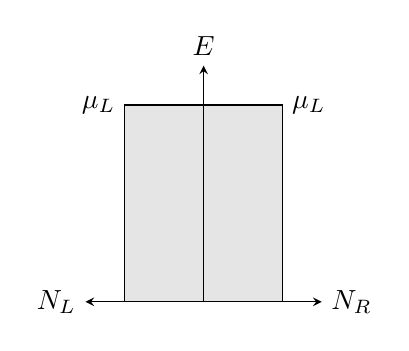
\begin{tikzpicture}
        %densità degli stati
        \draw[fill=gray!20!] (-1,0) rectangle (1,2.5);
        %assi
        \draw[-stealth] (0,0) -- (0,3) node[above] {$E$};
        \draw[stealth-stealth] (-1.5,0) node[left] {$N_L$}-- (1.5,0) node[right] {$N_R$};
        \node[left] at (-1,2.5) {$\mu_L$};
        \node[right] at (1,2.5) {$\mu_L$};
    \end{tikzpicture}
\end{figure}
\hspace{-0.6cm}L'Hamiltoniana descrive un processo in cui una particella viene distrutta da un lato e creata dall'altro, quindi un processo che trasferisce un elettrone da un elettrodo all'altro conservando l'energia.\\
Bisogna però verificare se, nell'altro elettrodo, siano disponibili livelli energetici liberi: se un livello è già occupato, l'elettrone non può occuparlo. Nella configurazione sopra illustrata il processo non è possibile, perché i due elettrodi sono identici, si trovano a temperatura nulla e tutti i livelli fino al livello di Fermi risultano occupati.\\
In questo caso, cioè in assenza di tensione applicata e a temperatura nulla, non può quindi avvenire tunneling: gli elettroni di un lead non possono passare nell'altro perché i corrispondenti livelli energetici sono già occupati, in accordo con il principio di esclusione di Pauli.\\
Che cosa accade invece se applichiamo una differenza di potenziale? Applicare una tensione significa, di fatto, traslare i livelli energetici dei due elettrodi:
\begin{figure}[H]
    \centering
    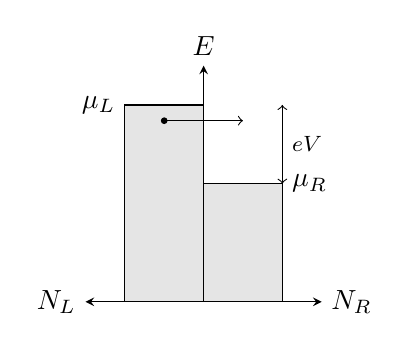
\begin{tikzpicture}
        %densità degli stati left lead
        \draw[fill=gray!20!] (-1,0) rectangle (0,2.5);
        %densità degli stati right lead
        \draw[fill=gray!20!] (0,0) rectangle (1,1.5);
        %assi
        \draw[-stealth] (0,0) -- (0,3) node[above] {$E$};
        \draw[stealth-stealth] (-1.5,0) node[left] {$N_L$}-- (1.5,0) node[right] {$N_R$};
        \node[left] at (-1,2.5) {$\mu_L$};
        \node[right] at (1,1.5) {$\mu_R$};

        %intensità del bias
        \draw[<->] (1,2.5) -- (1,1.5) node[midway,right] {\footnotesize$eV$};

        %elettrone che fa tunneling
        \filldraw (-0.5,2.3) circle (1pt);
        \draw[->] (-0.5,2.3) -- (0.5,2.3);
    \end{tikzpicture}
\end{figure}
\hspace{-0.6cm}Avremo quindi una densità degli stati traslata verso energie più alte da un lato e verso energie più basse dall'altro, in modo tale che i due potenziali chimici risultino separati da un'energia pari alla differenza di potenziale:
\begin{equation*}
    \mu_L - \mu_R = eV
\end{equation*}
In queste condizioni un elettrone nel lead sinistro può attraversare la barriera e occupare un livello energetico libero nel lead destro, proprio perché le due bande energetiche sono state traslate relativamente l'una rispetto all'altra.\\
Questo ci suggerisce immediatamente che, se calcoliamo la corrente che attraversa la giunzione, essa sarà nulla in assenza di tensione applicata, mentre diventerà diversa da zero quando esiste uno sbilancio tra le due bande energetiche, cioè quando viene applicata una differenza di potenziale.\\
Vediamo ora come scrivere esplicitamente tale corrente. Prima di tutto chiariamo la notazione utilizzata. Le energie $\varepsilon$ sono misurate rispetto al livello di Fermi di ciascun elettrodo, posto uguale a zero. Quindi $\varepsilon_L<0$ indica un livello occupato nell'elettrodo sinistro, mentre $\varepsilon_R>0$ indica un livello vuoto nell'elettrodo destro. La conservazione dell'energia richiede allora che
\begin{equation*}
    \varepsilon_R - \varepsilon_L
    =-eV
    =\mu_L - \mu_R
\end{equation*}
assumendo $e$ negativo.\\
L'idea è considerare l'Hamiltoniana di tunneling come una perturbazione rispetto alle Hamiltoniane dei due elettrodi, cioè assumere che i coefficienti $T_{\vb{k},\vb{q}}$, che quantificano l'interazione tra i due lead, siano molto più piccoli delle energie coinvolte:
\begin{equation*}
    |T_{\vb{k},\vb{q}}|
    \ll
    \varepsilon_{\vb{k},\sigma},
    \varepsilon_{\vb{q},\sigma}
\end{equation*}
Per determinare la probabilità per unità di tempo, cioè il rate, che un elettrone passi da un elettrodo all'altro a causa di questa perturbazione, utilizziamo la regola d'oro di Fermi. Dobbiamo quindi considerare tutte le possibili transizioni che conservano l'energia, la probabilità che lo stato iniziale sia occupato e quella che lo stato finale sia libero, sommando poi su tutti gli stati iniziali e finali possibili. Occorre inoltre includere un fattore 2 dovuto alla degenerazione di spin, poiché il processo non modifica lo spin.\\
L'espressione risultante è\mn{Con il simbolo $\sum_{R,L}$ intendiamo la somma su tutti i possibili valori di $\vb{q}$ e $\vb{k}$.}
\begin{equation*}
    \begin{split}
        W_{L \to R}
        &=
        2\frac{2\pi}{\hbar}
        \sum_{R,L}
        |T_{RL}|^2
        f_L(\varepsilon_L)
        \bigl[
            1-f_R(\varepsilon_R)
        \bigr]
        \delta(
            \varepsilon_L-eV-\varepsilon_R
        )
        \\
        W_{R \to L}
        &= 2\frac{2\pi}{\hbar} \sum_{R,L} |T_{RL}|^2 f_R(\varepsilon_R) \bigl[ 1 - f_L(\varepsilon_L) \bigr] \delta(\varepsilon_L - eV - \varepsilon_R)
    \end{split}
\end{equation*}
dove $f_L$ e $f_R$ sono le distribuzioni di Fermi dei due lead:
\begin{equation*}
    f_{\alpha}(\varepsilon_\alpha)
    =\frac{1}{1 + e^{\beta_\alpha \varepsilon_\alpha}}
    \qq{,}
    \alpha=L,R
\end{equation*}
Notiamo che stiamo esplicitamente indicando il lead perché, in generale, i due elettrodi possono trovarsi a temperature differenti. Se invece le temperature coincidono, possiamo semplicemente scrivere $f(\varepsilon)$ senza specificare il lead, perché in quel caso conta soltanto l'energia.\\
Una volta ottenute le probabilità di tunneling, possiamo ricavare facilmente la corrente totale, che è semplicemente la carica del portatore, $-e$, moltiplicata per la differenza tra i due rate:
\begin{equation*}
    I = -e ( W_{L \to R} - W_{R \to L} )
\end{equation*}
Sostituendo le espressioni esplicite dei due rate, otteniamo
\begin{equation*}
    I = -e \frac{4\pi}{\hbar} \sum_{R,L} |T_{RL}|^2 \bigl[ f_L(\varepsilon_L) - f_R(\varepsilon_R) \bigr] \delta( \varepsilon_L-eV-\varepsilon_R )
\end{equation*}
Passiamo ora al limite del continuo, sostituendo le somme con integrali sulle energie dei due lead e introducendo le corrispondenti densità degli stati $N_L(\varepsilon_L)$ e $N_R(\varepsilon_R)$:
\begin{equation*}
    I = -e \frac{4\pi}{\hbar} \int \dd{\varepsilon_R} N_R \int \dd{\varepsilon_L} N_L |T_{RL}|^2 \bigl[ f_L(\varepsilon_L) - f_R(\varepsilon_R) \bigr] \delta( \varepsilon_L-eV-\varepsilon_R )
\end{equation*}
Usando la delta di Dirac rimane un solo integrale, ad esempio su $\varepsilon_R$, mentre $\varepsilon_L$ viene sostituita con il valore imposto dalla conservazione dell'energia:
\begin{equation*}
    \varepsilon_L=eV+\varepsilon_R
\end{equation*}
Otteniamo quindi
\begin{equation*}
    I = -e \frac{4\pi}{\hbar} \int \dd{\varepsilon_R} N_R N_L |T_{RL}|^2
    \bigl[ f_L(eV+\varepsilon_R) - f_R(\varepsilon_R) \bigr]
\end{equation*}
Se assumiamo che la densità degli stati e l'ampiezza di tunneling siano praticamente costanti attorno al livello di Fermi, possiamo portarli fuori dall'integrale. Rimane così soltanto l'integrale della differenza delle due funzioni di Fermi:
\begin{equation*}
    \int \dd{\varepsilon_R} \bigl[ f_L(eV+\varepsilon_R) - f_R(\varepsilon_R) \bigr] = eV
\end{equation*}
È facile comprendere questo risultato graficamente a temperatura nulla:
\begin{figure}[H]
    \centering
    \begin{tikzpicture}
        %assi
        \draw[-stealth] (0,0) -- (0,2) node[left] {$f$};
        \draw[-stealth] (0,0) -- (5,0) node[right] {$\varepsilon$};
        \fill[pattern=north east lines] (2.3,0) rectangle (3.7,1.5);

        %fermi function left lead
        \draw[thick, blue]
        (0,1.5)
        --
        (3.7,1.5)
        node[midway, above] {\hspace{2cm}\footnotesize$f_R$}
        --
        (3.7,0)
        node[black, below] {\footnotesize$\varepsilon_R + eV$};

        \draw[thick, red]
        (0,1.5)
        --
        (2.3,1.5)
        node[midway, above] {\footnotesize$f_L$}
        --
        (2.3,0)
        node[black, below] {\footnotesize$\varepsilon_R$};
    \end{tikzpicture}
\end{figure}
\hspace{-0.6cm}Come si vede, la differenza tra le due funzioni di Fermi corrisponde semplicemente alla regione tratteggiata, che è un rettangolo di base $eV$ e altezza unitaria; l'integrale vale quindi semplicemente $eV$.\\
Tornando allora all'espressione della corrente, otteniamo\mn{È evidente che in tutto questo discorso non tornano i segni.}
\begin{equation*}
    I
    =\frac{4\pi e^2}{\hbar}N_LN_R|T_{RL}|^2V
    \equiv G_{NN}V
\end{equation*}
Si tratta semplicemente della legge di Ohm: la corrente è proporzionale alla differenza di potenziale applicata, con coefficiente di proporzionalità dato dalla conduttanza $G_{NN}$.\\
Questa è quindi una maniera di recuperare la legge di Ohm partendo da una descrizione microscopica quantistica degli elettroni nei due elettrodi. Ne segue che la caratteristica corrente--tensione della giunzione è lineare, con una pendenza determinata dalla conduttanza $G_{NN}$, che risulta proporzionale alla densità degli stati nei due lead e al quadrato dell'ampiezza di tunneling.
\subsection{Lead superconduttivi}
Vediamo ora che cosa accade quando i lead sono superconduttivi.\\
Consideriamo innanzitutto un processo di tunneling di singolo elettrone, cioè il passaggio di un singolo elettrone attraverso la giunzione. Perché un tale processo possa avvenire, è necessario rompere una coppia di Cooper, dalla quale otteniamo due elettroni. Come abbiamo già visto il costo energetico associato a ciò è pari a $2\Delta$, perché i livelli disponibili per ciascun elettrone si trovano a un'energia $\Delta$ sopra lo stato fondamentale.\\
Dobbiamo allora riesprimere tale stato elettronico in termini delle opportune eccitazioni del superconduttore. Esprimiamo allora l'operatore di creazione dell'elettrone $c^{\dag}_{\vb{k},\uparrow}$ in termini degli operatori di creazione e distruzione delle eccitazioni:
\begin{equation*}
    c^{\dag}_{\vb{k},\uparrow}
    =
    u^{\vphantom{\dag}}_{\vb{k}} b^{\dag}_{\vb{k},\uparrow}
    +
    \nu^{\vphantom{\dag}}_{\vb{k}} b^{\vphantom{\dag}}_{-\vb{k},\downarrow}
\end{equation*}
Se il superconduttore si trova nel suo stato fondamentale, il secondo termine fornisce un contributo nullo e il processo genera una corrente proporzionale a $|u_{\vb{k}}|^2 |T_{\vb{k},\vb{q}}|^2$.\\
Il significato fisico del fattore $|u_{\vb{k}}|^2$ è che esso rappresenta la probabilità che lo stato $\ket*{\vb{k}}$ non sia occupato nella funzione d'onda BCS e che quindi possa accogliere un elettrone incidente.\\
A prima vista sembrerebbe quindi che la corrente di tunneling dipenda sia dalla natura dello stato fondamentale superconduttivo sia dalla densità degli stati eccitati disponibili. Tuttavia ciò non è corretto.\\
Ricordiamo che le eccitazioni possiedono una dispersione parabolica. Se fissiamo un certo valore di $E_{\vb{k}}$, lo stesso valore dell'energia può essere ottenuto sia per $\xi_{\vb{k}}$ che per $-\xi_{\vb{k}}$. In altre parole, a causa della struttura dello spettro delle eccitazioni, possiamo avere due eccitazioni, che indichiamo con $E_{\vb{k}}$ ed $E_{\vb{k}'}$, coincidenti quando $\xi_{\vb{k}'}=-\xi_{\vb{k}}$.\\
Se allora adesso consideriamo l'operatore di creazione dell'elettrone $c^{\dag}_{\vb{k}',\uparrow}$, che crea un elettrone nello stato a singola particella $(\vb{k}',\uparrow)$, e analogamente a prima lo esprimiamo in termini degli operatori di creazione e distruzione delle eccitazioni, è facile vedere che il tunneling verso $\vb{k}'$ contribuisce con una corrente proporzionale a $|u_{\vb{k}'}|^2 |T_{\vb{k}',\vb{q}}|^2$.\\
Se però adesso utilizziamo l'\eqrefcustom{eq:coefficiente_u_BCS} e l'\eqrefcustom{eq:coefficiente_nu_BCS}, osserviamo che si ha
\begin{equation*}
    |u_{\vb{k}'}|^2
    =\frac{1}{2} \biggl( 1 + \frac{ \xi_{\vb{k}'} }{ \sqrt{ \xi_{\vb{k}'}^2+|\Delta|^2 } } \biggr)
    =\frac{1}{2} \biggl( 1 - \frac{ \xi_{\vb{k}} }{ \sqrt{ \xi_{\vb{k}}^2+|\Delta|^2 } } \biggr)
    \equiv |\nu_{\vb{k}}|^2
\end{equation*}
dove $|\nu_{\vb{k}}|^2$ rappresenta la probabilità che tale livello sia occupato nello stato fondamentale BCS.\\
Possiamo inoltre assumere ragionevolmente che $|T_{\vb{k},\vb{q}}|^2 = |T_{\vb{k}',\vb{q}}|^2$, dato che $k$ e $k'$ si trovano entrambi nelle vicinanze dello stesso punto della superficie di Fermi.\\
Questo significa che la probabilità che il livello corrispondente a $\vb{k}'$ sia libero per il tunneling coincide con la probabilità che lo stato con $\xi$ opposto sia occupato:
\begin{equation}
    |u_{\vb{k}'}|^2
    |T_{\vb{k}'\vb{q}}|^2
    =
    |\nu_{\vb{k}}|^2
    |T_{\vb{k}\vb{q}}|^2
    \label{eq:probability_tunneling_k'}
\end{equation}
Di conseguenza, se vogliamo valutare la probabilità totale che esista uno stato disponibile corrispondente a un certo valore di $\vb{k}$, dobbiamo sommare il contributo $|u_{\vb{k}}|^2 |T_{\vb{k},\vb{q}}|^2$, associato a $\xi_{\vb{k}}$, con il contributo $|u_{\vb{k}'}|^2 |T_{\vb{k}',\vb{q}}|^2$.\\
Esistono quindi due processi indipendenti, che derivano direttamente dalla particolare struttura dello spettro delle eccitazioni superconduttive. Complessivamente, la probabilità che un singolo elettrone venga trasferito nello stato a singola particella $(\vb{k},\uparrow)$, quando il superconduttore si trova nello stato fondamentale BCS, è data da
\begin{equation*}
    |u_{\vb{k}}|^2 |T_{\vb{k},\vb{q}}|^2 + |u_{\vb{k}'}|^2 |T_{\vb{k}',\vb{q}}|^2
\end{equation*}
Usando l'\eqrefcustom{eq:probability_tunneling_k'}, possiamo riscrivere questa espressione come
\begin{equation*}
    ( |u_{\vb{k}}|^2 + |\nu_{\vb{k}}|^2 ) |T_{\vb{k},\vb{q}}|^2
    =|T_{\vb{k},\vb{q}}|^2
\end{equation*}
dove abbiamo utilizzato la condizione di normalizzazione dello stato fondamentale BCS, $|u_{\vb{k}}|^2 + |\nu_{\vb{k}}|^2 = 1$.\\
Questa è una conseguenza notevole, perché ci dice che la corrente di tunneling risultante non dipende esplicitamente dai coefficienti che compaiono nello stato fondamentale BCS, ma soltanto dall'ampiezza di tunneling.
\subsection{Modello a semiconduttore per un superconduttore}
Quest'ultima osservazione è particolarmente importante, perché il passo successivo consiste nel valutare la corrente. Per farlo dobbiamo applicare la regola d'oro di Fermi e costruire un quadro analogo a quello introdotto nel caso dei metalli normali.\\
Questo tipo di descrizione viene spesso chiamato \emph{modello a semiconduttore} del superconduttore: quando si studiano le correnti nei dispositivi superconduttivi, si considera infatti la densità degli stati e i possibili processi di tunneling da un lato all'altro della giunzione, tenendo conto del gap energetico. Nel caso di un metallo normale questo procedimento è semplice, perché la densità degli stati ha una struttura molto semplice. Nel caso di un superconduttore, invece, la situazione è più complessa: nello stato fondamentale BCS gli elettroni formano coppie di Cooper e, quando tali coppie vengono rotte, compaiono le quasiparticelle, che possiedono una propria densità degli stati.\\
Quando consideriamo la corrente di tunneling dobbiamo necessariamente coinvolgere questi stati eccitati, perché il tunneling di singolo elettrone richiede la rottura di una coppia di Cooper e bisogna quindi capire in quali stati possano andare gli elettroni risultanti dalla rottura della coppia.\\
Il fatto che i processi di tunneling associati alla rottura di una coppia di Cooper non dipendano esplicitamente dai coefficienti che compaiono nello stato fondamentale BCS implica che, se vogliamo costruire una descrizione analoga a quella utilizzata per i semiconduttori, possiamo utilizzare un modello che coinvolga soltanto i livelli energetici eccitati, senza mantenere memoria esplicita dello stato fondamentale BCS.\\
Questo modello, utilizzato esclusivamente per descrivere i processi di tunneling elettronico, prende il nome di \emph{modello a semiconduttore per un superconduttore}. Vediamo qualitativamente come funziona:
\begin{figure}[H]
    \centering
    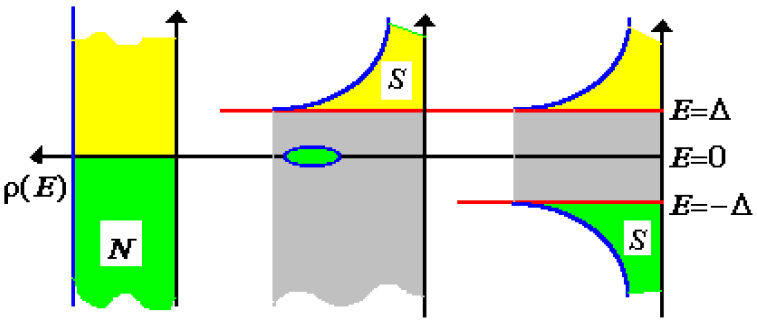
\includegraphics[width=0.8\textwidth]{immagini/semiconductor_model.png}
    \caption*{Rappresentazione a singola particella della densità degli stati di un superconduttore: quasiparticelle libere appartenenti a due bande. Una banda di coppie legate a energia $\Delta$ sotto il livello di Fermi e una banda di ``coppie rotte'' a energia $\Delta$ sopra il livello di Fermi. Rompere una coppia significa eccitare una quasiparticella sopra il gap. Il costo energetico per creare una ``lacuna'' nella banda inferiore e una quasiparticella nella banda superiore è pari a $2\Delta$.}
\end{figure}
\hspace{-0.6cm}A sinistra vediamo la struttura degli stati di un metallo normale: tutti i livelli fino al livello di Fermi (assunto come zero dell'energia) sono occupati, mentre quelli sopra il livello di Fermi sono vuoti.\\
Nel caso del superconduttore sappiamo invece che la densità degli stati possiede l'andamento caratteristico già discusso: compare un gap energetico e, vicino ai bordi del gap, la densità degli stati diverge prima di decrescere nuovamente.\\
L'immagine sulla destra rappresenta proprio il modello a semiconduttore del superconduttore. In essa compare la dipendenza delle energie eccitate dall'energia, ma — almeno a temperatura nulla — tali stati non sono occupati, perché tutte le particelle si trovano condensate nello stato fondamentale BCS.\\
Osserviamo inoltre che in questa rappresentazione lo stato fondamentale BCS non compare esplicitamente.\mn{Nel quadro a singola particella l'energia dello stato fondamentale BCS non compare nemmeno nel diagramma dei livelli energetici. Si tratta di un modello estremamente semplificato, utile esclusivamente per descrivere processi di tunneling a singolo elettrone, che risultano ``orizzontali'' quando i potenziali chimici dei due metalli vengono traslati per tenere conto della differenza di potenziale applicata.}
Un modo schematico per ricordare l'esistenza dello stato fondamentale è il ``blob'' rappresentato attorno all'energia zero nella figura centrale: esso indica semplicemente che tutti gli elettroni si trovano condensati altrove, cioè nello stato BCS. Le coppie di Cooper non partecipano direttamente al processo di tunneling di singolo elettrone.\\
Nel modello a semiconduttore ciò che si fa è passare dalla densità delle eccitazioni a una densità degli stati ottenuta riproducendo specularmente, anche per energie negative, la densità degli stati delle eccitazioni superconduttive. L'idea è quindi descrivere gli elettroni che formano lo stato fondamentale BCS come una sorta di mare di Fermi di stati occupati al di sotto del gap energetico.\\
Per capire perché questa costruzione abbia senso, immaginiamo di diminuire progressivamente il valore del gap $\Delta$ fino a portarlo a zero. Se partiamo da una densità degli stati superconduttiva e ne consideriamo la riproduzione speculare anche per energie negative, vediamo che, nel limite $\Delta \to 0$, il gap si chiude e la divergenza ai bordi scompare: la densità degli stati tende semplicemente a un valore costante uguale a quello di un metallo normale. In altre parole, se immaginassimo di osservare questo processo come un filmato, passando gradualmente da un valore finito di $\Delta$ fino a $\Delta=0$, vedremmo il diagramma trasformarsi gradualmente nella struttura tipica di un metallo normale.\\
Questo è il motivo per cui, nel modello a semiconduttore, si introduce una copia speculare della densità degli stati superconduttiva anche per energie negative: in questo modo il modello si riconduce naturalmente al caso normale quando il gap tende a zero.\\
Utilizzeremo questa rappresentazione per descrivere i processi di corrente di tunneling, in maniera analoga a quanto si fa nei semiconduttori. Anche nei semiconduttori, infatti, il trasporto è descritto in termini di quasiparticelle (elettroni e lacune) e la corrente deriva da processi di annichilazione di particelle da un lato e creazione dall'altro. Dal punto di vista concettuale, i processi che stiamo considerando qui sono dello stesso tipo.
\subsection{Giunzione Normale--Isolante--Superconduttore (NIS)}
Vediamo ora come utilizzare questo modello a semiconduttore per derivare la corrente tunnel. Il primo caso che consideriamo è una giunzione formata da un lead normale, uno strato isolante e un superconduttore. Se utilizziamo il modello a semiconduttore, il diagramma della densità degli stati assume la forma seguente:
\begin{figure}[H]
    \centering
    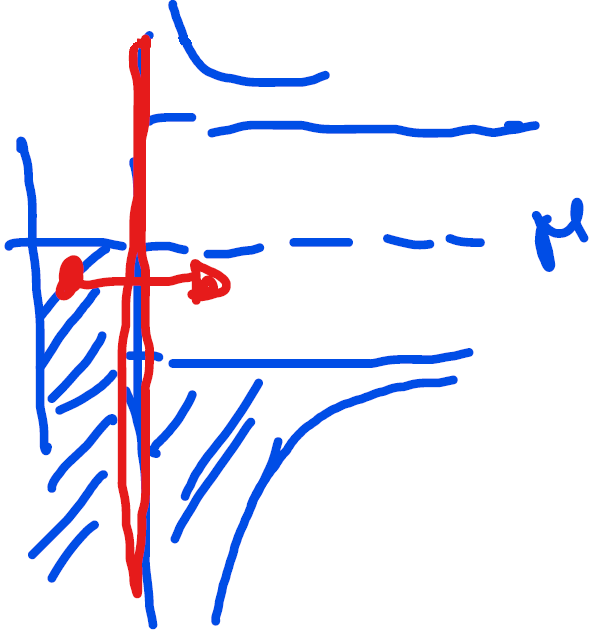
\includegraphics[width=0.3\textwidth]{immagini/NIS_junction_no_bias.png}
    \hspace{1cm}
    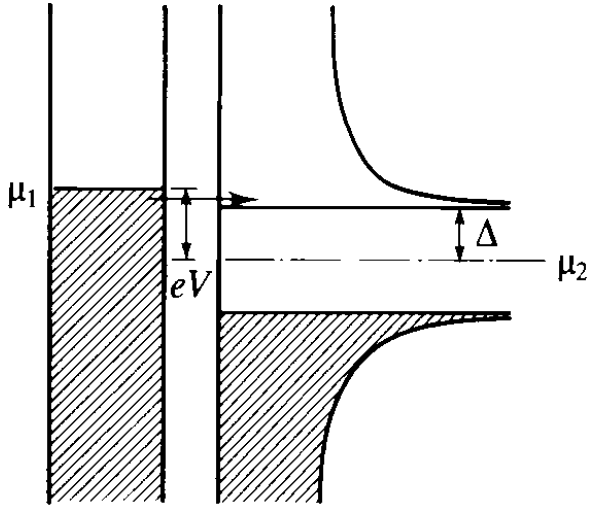
\includegraphics[width=0.4\textwidth]{immagini/NIS_junction.png}
    \caption*{(a) Tunneling N-S a $T=0$ in assenza di tensione applicata. (b) Tunneling N-S a $T=0$, con tensione di bias appena superiore alla soglia di conduzione, cioè con $eV$ leggermente maggiore del gap energetico $\Delta$. La freccia orizzontale rappresenta elettroni provenienti dal lato sinistro che tunnelano verso stati vuoti sul lato destro.}
\end{figure}
\hspace{-0.6cm}Sul lato sinistro abbiamo il metallo normale, mentre sul lato destro il superconduttore. Si noti che è stata applicata una tensione che trasla le due bande energetiche, perché altrimenti la situazione sarebbe quella mostrata nella figura (a). In queste condizioni non avremmo alcuna corrente, perché un elettrone presente nel metallo normale non potrebbe passare dall'altro lato: nel superconduttore non esistono infatti livelli disponibili a causa del gap energetico.\\
Possiamo avere una corrente soltanto applicando una differenza di potenziale, come nella figura (b), in modo da traslare le bande del superconduttore verso energie più basse e rendere possibili transizioni orizzontali dal metallo normale al superconduttore. In questo caso ciascun elettrone del metallo normale vede infatti un livello di quasiparticella disponibile nel superconduttore.\\
Devono quindi essere soddisfatte due condizioni:
\begin{itemize}[leftmargin=0.5cm]
    \item il livello energetico deve esistere;
    \item tale livello deve essere vuoto, in modo che l'elettrone possa occuparlo.
\end{itemize}
Questo implica immediatamente che nella caratteristica $I$--$V$ non osserveremo corrente per valori arbitrariamente piccoli della tensione applicata: è necessario che la tensione sia sufficientemente grande da permettere il tunneling di un elettrone. In altre parole, finché $eV<\Delta$ non avremo corrente; quando invece $eV$ supera $\Delta$, la corrente può iniziare a fluire.\\
Vediamo ora come si ottiene questo risultato. Utilizziamo ancora lo stesso modello per l'Hamiltoniana di tunneling e descriviamo la corrente tramite i rate di transizione $W_{L \to R}$ e $W_{R \to L}$ ottenuti con la regola d'oro di Fermi. La corrente totale sarà quindi
\begin{equation*}
    I_{NS}
    =
    I_{N \to S}
    -
    I_{S \to N}
\end{equation*}
Cominciamo valutando il primo termine, cioè la corrente che fluisce dal metallo normale al superconduttore. Sottolineiamo che qui non intervengono coppie di Cooper: compaiono soltanto quasiparticelle, che obbediscono alla statistica di Fermi e la cui occupazione è descritta dalla distribuzione di Fermi.\\
Procedendo esattamente come nel caso precedente, otteniamo\mn{Rispetto alle slide ho riportato una modifica. Infatti lì compare esplicitamente il fattore con la radice derivante dalla DOS del superconduttore, ma compare anche $N_R(E_R)$. Siccome $N_R$ dipende da $E_R$ solo se al suo interno c'è la radice, allora è più chiaro scrivere direttamente $N_R(E_R)$, che è la densità degli stati del superconduttore, invece di scrivere la radice e poi $N_R$.}
\begin{equation*}
    \begin{split}
        I_{N \to S}
        &=
        -e
        \frac{4\pi}{\hbar}
        \int
        \dd{\varepsilon_L}
        \int
        \dd{E_R}
        \Bigl\{
            |T_{LR}|^2
            N_L(\varepsilon_L)
            f_L(\varepsilon_L)
        \Bigr.
        \\
        & \hphantom{=
        -e
        \frac{4\pi}{\hbar}
        \int
        \dd{\varepsilon_L}
        \int
        \dd{E_R}}
        \Bigl.
        \times
        N_R(E_R)
        \bigl[
            1-f_R(E_R)
        \bigr]
        \delta(
            \varepsilon_L-eV-E_R
        )
        \Bigr\}
    \end{split}
\end{equation*}
Osserviamo che stiamo usando simboli differenti per i due lead: sul lato sinistro abbiamo un metallo normale e utilizziamo quindi la notazione $\varepsilon_L$, mentre sul lato destro abbiamo le eccitazioni del superconduttore, indicate con $E_R$.\\
Dobbiamo inoltre considerare la densità degli stati nei due lead. Per il metallo normale abbiamo semplicemente $N_L(\varepsilon_L)$, mentre per il superconduttore dobbiamo usare la densità degli stati delle quasiparticelle:
\begin{equation*}
    N_R(E_R)
    =
    N_R(0)
    \frac{
        E_R
    }{
        \sqrt{
            E_R^2-\Delta^2
        }
    }
\end{equation*}
Dobbiamo poi includere i consueti fattori che selezionano gli stati inizialmente occupati e quelli finali disponibili. Gli stati inizialmente occupati sono descritti dal prodotto $N_L(\varepsilon_L)
f_L(\varepsilon_L)$, mentre gli stati finali disponibili sono descritti da $N_R(E_R) \bigl[ 1-f_R(E_R) \bigr]$.\\
Questa è soltanto la corrente che fluisce dal metallo normale al superconduttore. Se consideriamo il processo inverso, cioè il contributo alla corrente dal superconduttore verso il metallo normale, dobbiamo semplicemente scambiare il ruolo degli stati occupati e vuoti:
\begin{equation*}
    \begin{split}
        I_{S \to N}
        &=
        -e
        \frac{4\pi}{\hbar}
        \int
        \dd{\varepsilon_L}
        \int
        \dd{E_R}
        \Bigl\{
            |T_{LR}|^2
            N_L(\varepsilon_L)
            \bigl[
                1-f_L(\varepsilon_L)
            \bigr]
        \Bigr.
        \\
        & \hphantom{=
        -e
        \frac{4\pi}{\hbar}
        \int
        \dd{\varepsilon_L}
        \int
        \dd{E_R}}
        \Bigl.
        \times
        N_R(E_R)
        f_R(E_R)
        \delta(
            \varepsilon_L-eV-E_R
        )
        \Bigr\}
    \end{split}
\end{equation*}
La corrente totale risulta quindi
\begin{equation*}
    \begin{split}
        I_{NS}
        &=
        -e
        \frac{4\pi}{\hbar}
        \int
        \dd{\varepsilon_L}
        \int
        \dd{E_R}
        \Bigl\{
            |T_{LR}|^2
            N_L(\varepsilon_L)
            N_R(E_R)
        \Bigr.
        \\
        & \hphantom{=
        -e
        \frac{4\pi}{\hbar}
        \int
        \dd{\varepsilon_L}
        \int
        \dd{E_R}}
        \Bigl.
        \times
        \bigl[
            f_L(\varepsilon_L)
            -
            f_R(E_R)
        \bigr]
        \delta(
            \varepsilon_L-eV-E_R
        )
        \Bigr\}
    \end{split}
\end{equation*}
Usando la delta di Dirac possiamo eliminare uno dei due integrali, ad esempio quello su $\varepsilon_L$, ottenendo un integrale soltanto su $E_R$.\\
Inoltre, scrivendo esplicitamente la densità degli stati del superconduttore, otteniamo
\begin{equation*}
    \begin{split}
        I_{NS}
        &=
        -e
        \frac{4\pi}{\hbar}
        |T_{LR}|^2
        N_L(0)
        N_R(0)
        \\
        & \hphantom{=}
        \times
        \int_{-\infty}^{+\infty}
        \dd{E_R}
        \frac{
            E_R
        }{
            \sqrt{
                E_R^2-\Delta^2
            }
        }
        \bigl[
            f_L(eV+E_R)
            -
            f_R(E_R)
        \bigr]
    \end{split}
\end{equation*}
dove abbiamo assunto che l'ampiezza di tunneling e la densità degli stati siano praticamente costanti attorno al livello di Fermi.\\
A temperatura nulla, le funzioni di Fermi selezionano gli stati energetici compresi in una finestra di ampiezza $eV$. Tuttavia, nel superconduttore gli stati disponibili non iniziano da energia zero, ma da $\Delta$, perché la densità degli stati si annulla al di sotto del gap.\mn{Infatti, in principio le due funzioni di Fermi selezionano energie comprese tra zero e $-eV$, ma poiché la densità degli stati del superconduttore è nulla per energie minori di $\Delta$, rimane soltanto l'integrale compreso tra $\Delta$ e $-eV$.} Otteniamo quindi
\begin{equation*}
    \begin{split}
        I_{NS}
        &\approx
        -e
        \frac{4\pi}{\hbar}
        |T_{LR}|^2
        N_L(0)
        N_R(0)
        \int_{\Delta}^{-eV}
        \dd{E_R}
        \frac{
            E_R
        }{
            \sqrt{
                E_R^2-\Delta^2
            }
        }
        \\
        &=
        \frac{
            G_{NN}
        }{
            |e|
        }
        \sqrt{
            (eV)^2-\Delta^2
        }.
    \end{split}
\end{equation*}
Vediamo quindi che il risultato dell'integrale possiede un andamento a radice quadrata dipendente sia dal gap $\Delta$ sia dalla tensione applicata. A temperatura nulla, tale comportamento inizia soltanto quando $eV=\Delta$, come mostrato nella figura seguente:
\begin{figure}[H]
    \centering
    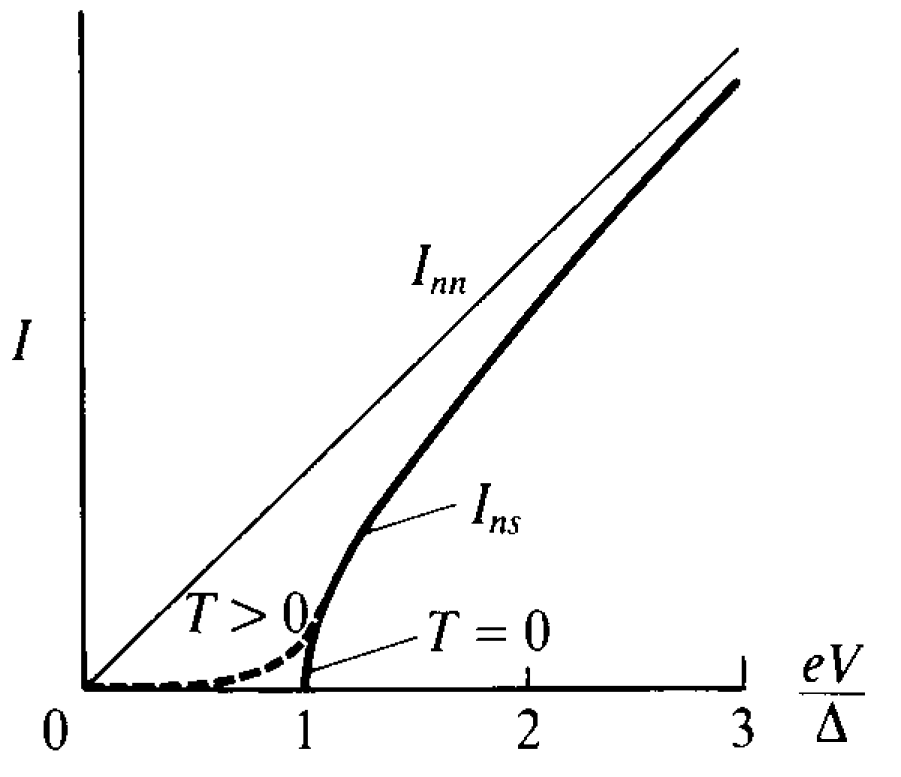
\includegraphics[width=0.45\textwidth]{immagini/IV_NIS.png}
\end{figure}
\hspace{-0.6cm}Come si vede, per $eV \gg \Delta$ si recupera nuovamente un comportamento lineare\mn{In tale regime il termine $\Delta$ all'interno della radice diventa trascurabile e si ottiene $\sqrt{(eV)^2}=eV$.}.\\
L'aspetto notevole è che il coefficiente davanti all'integrale è esattamente lo stesso che compare nella corrente quando entrambi i lead si trovano nello stato normale. Questo significa che, se la tensione applicata è molto maggiore del gap energetico, il sistema si comporta sostanzialmente come un metallo normale: la caratteristica $I$--$V$ torna lineare e con la stessa pendenza.\\
Riducendo invece la tensione applicata, la corrente risulta più piccola rispetto al caso normale e dipende in maniera non lineare da $eV$. Inoltre, per tensioni tali che $eV/\Delta<1$, la corrente si annulla completamente.\\
A temperatura finita la situazione cambia leggermente, perché in questo caso possono comparire stati occupati sopra il gap e stati vuoti al di sotto di esso, come illustrato nella figura seguente:
\begin{figure}[H]
    \centering
    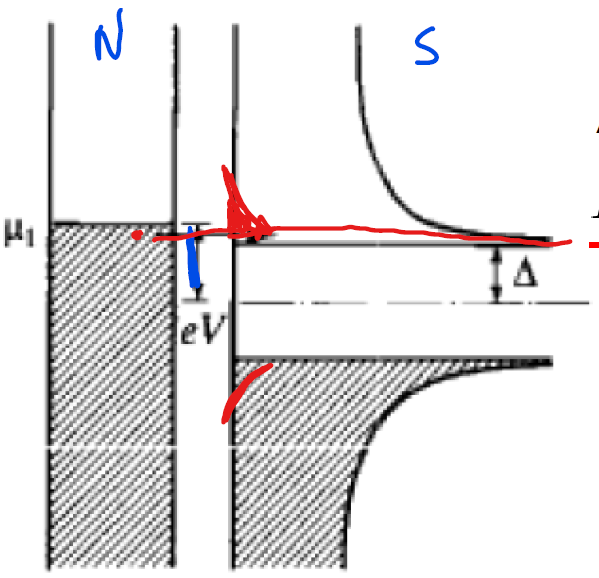
\includegraphics[width=0.4\textwidth]{immagini/finite_temperature_NIS.png}
\end{figure}
\hspace{-0.6cm}Analogamente a quanto avviene nei semiconduttori, a temperatura finita esistono livelli eccitati termicamente occupati. Ciò significa che possono verificarsi processi di tunneling anche per tensioni minori di $\Delta$.\\
Questo spiega perché nella caratteristica $I$--$V$ compare una piccola corrente anche per $eV<\Delta$, rappresentata nella figura dalla linea tratteggiata.\\
Possiamo anche valutare la conduttanza differenziale, che non è altro che la derivata della corrente rispetto alla tensione. Per $T=0$ si ottiene
\begin{equation*}
    \begin{split}
        \dv{I_{NS}}{V}
        &=
        e
        \frac{4\pi}{\hbar}
        N_L(0)
        |T_{LR}|^2
        \frac{N_R(0)|e|V}{\sqrt{(eV)^2-\Delta^2}}
    \end{split}
\end{equation*}
Osserviamo che questa funzione possiede essenzialmente la stessa forma funzionale della densità degli stati del superconduttore, con l'unica differenza che al numeratore compare $eV$ invece di $E$.\\
Questo significa che, se rappresentiamo la conduttanza differenziale in funzione di $eV/\Delta$, otteniamo un andamento identico a quello della densità degli stati del superconduttore, naturalmente valido soltanto per $eV>\Delta$:
\begin{figure}[H]
    \centering
    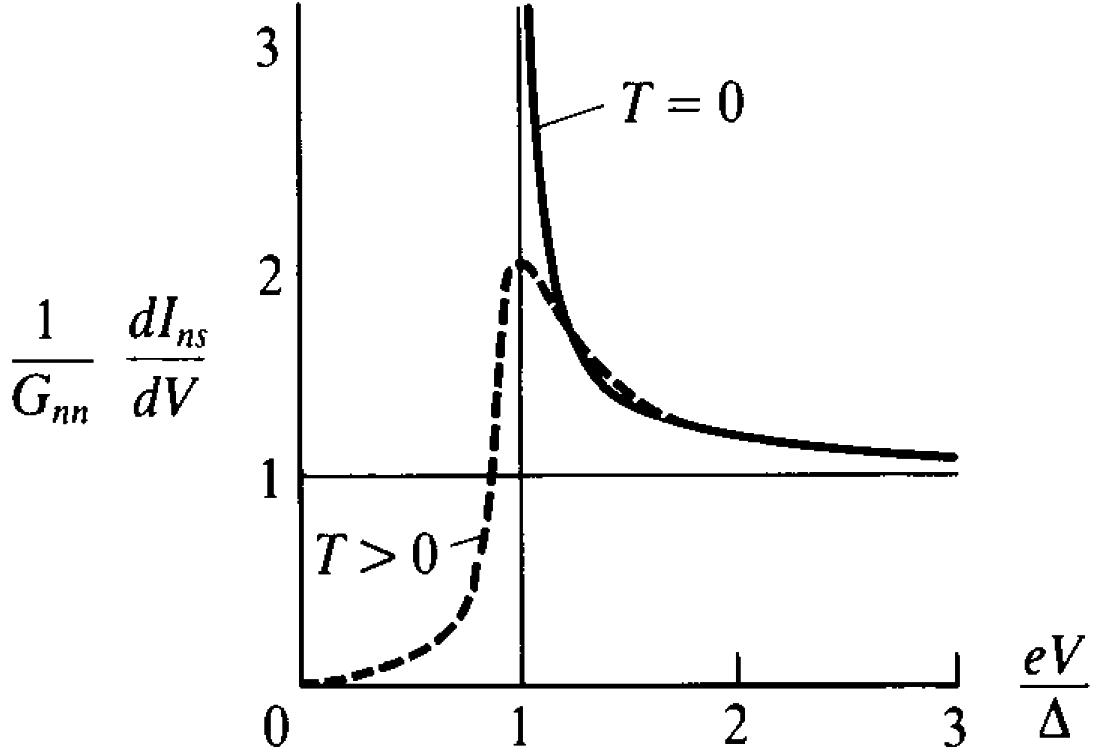
\includegraphics[width=0.5\textwidth]{immagini/differential_conductance_NIS.png}
\end{figure}
\hspace{-0.6cm}Idealmente, se fosse possibile lavorare esattamente a temperatura nulla, dalla misura della conduttanza differenziale potremmo ricavare direttamente la densità degli stati del superconduttore.\\
Naturalmente, negli esperimenti reali ci troviamo sempre a temperatura finita. Gli effetti termici modificano leggermente la regione con $eV/\Delta>1$ ed eliminano la divergenza che comparirebbe a temperatura nulla. In pratica, il comportamento della conduttanza differenziale rimane molto simile a quello ideale, ma il picco divergente viene sostituito da un massimo finito e smussato, che decresce rapidamente per tensioni più piccole.\\
Questo significa che, effettuando un esperimento di tunneling a temperature sufficientemente inferiori al gap, si osserva una conduttanza differenziale che riproduce molto bene la densità degli stati di un superconduttore, eccetto per la divergenza ideale.\\
\mn{Questa parte l'ho presa da \cite{Tinkham} e la aggiungo solo per completezza. La prof a lezione mostra solo l'espressione.}
Vediamo matematicamente da dove nasce questo comportamento non monotono. Consideriamo la conduttanza differenziale $\dv*{I}{V}$ in funzione della tensione:
\begin{equation*}
    G_{ns}
    =
    \dv{I_{ns}}{V}
    =
    G_{nn}
    \int_{-\infty}^{\infty}
    \dd{E}
    \frac{
        N_R(E)
    }{
        N_L(0)
    }
    \qty(
        -
        \pdv{
            f(E+eV)
        }{
            eV
        }
    ).
\end{equation*}
Poiché $-\pdv*{f(E+eV)}{eV}$ è una funzione a campana centrata attorno a $E=-eV$, con larghezza dell'ordine di $\sim 4kT$ e area unitaria, a temperatura finita la conduttanza misura in pratica una densità degli stati ``spalmata'' su un intervallo energetico dell'ordine di $\pm 2kT$, proprio a causa della larghezza della funzione peso.
\subsection{Giunzione Superconduttore--Isolante--Superconduttore (SIS)}
Consideriamo ora ill caso in cui entrambi i lead siano superconduttivi.\\
L'idea si comprende facilmente osservando la seguente struttura a bande. Ancora una volta, il punto fondamentale è che possiamo avere una corrente di tunneling soltanto se esistono stati occupati da un lato e stati vuoti dall'altro.
\begin{figure}[H]
    \centering
    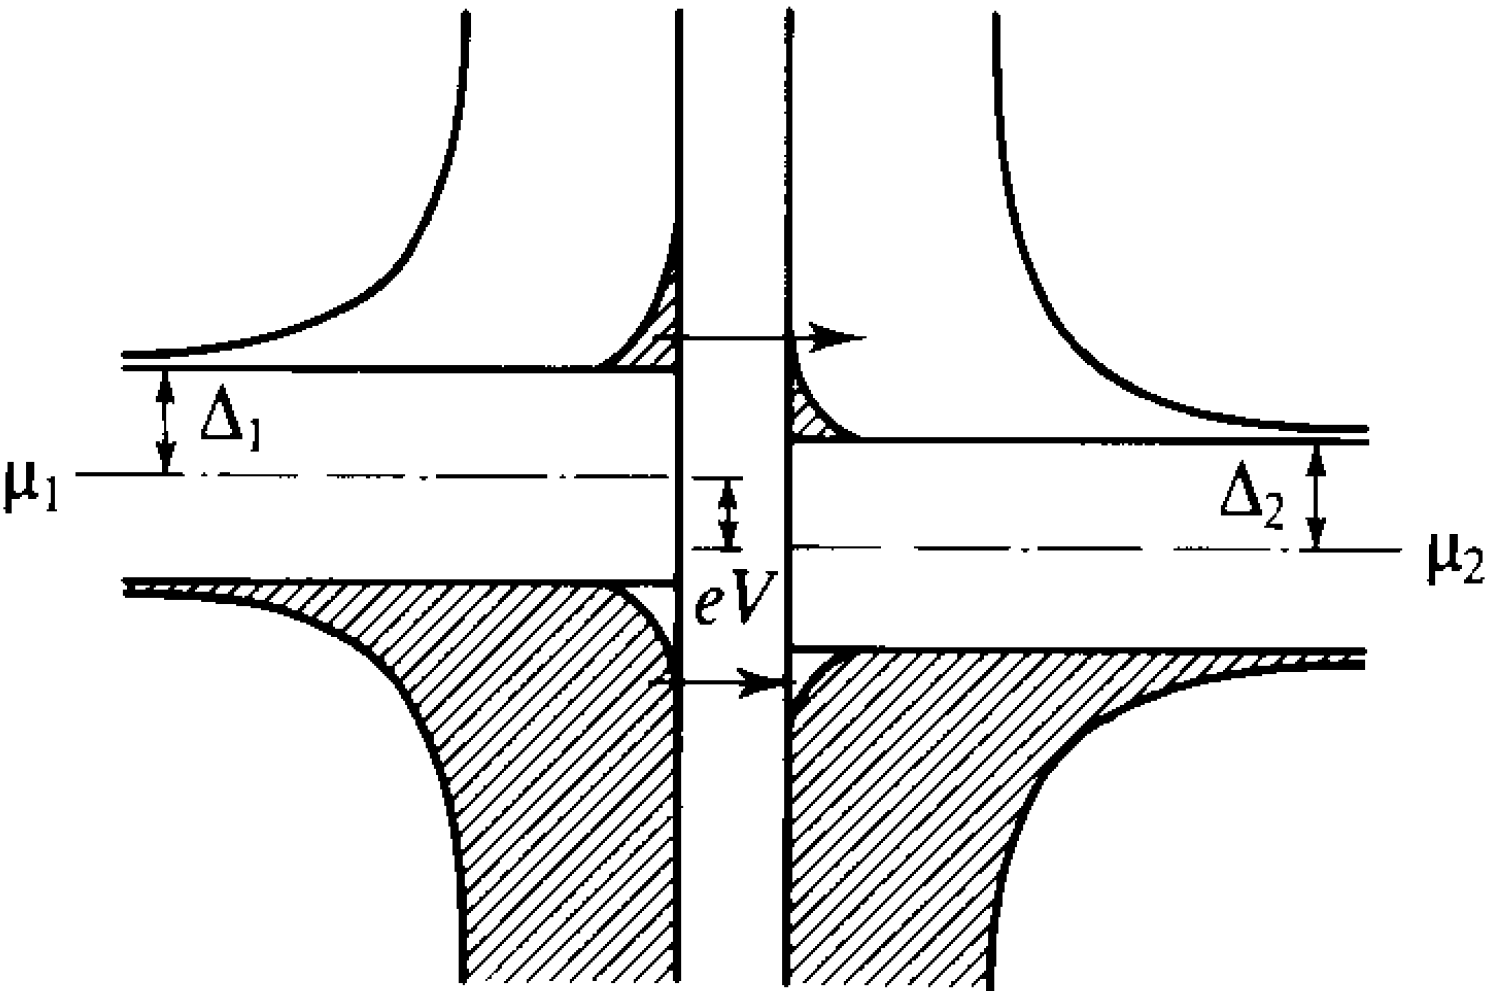
\includegraphics[width=0.55\textwidth]{immagini/SIS_junction.png}
\end{figure}
\hspace{-0.6cm}Questa figura rappresenta il caso di temperatura piccola ma finita: vicino alla sommità di quella che sarebbe la banda di valenza compaiono infatti alcuni livelli non occupati, mentre nel fondo della banda superiore si osservano alcune quasiparticelle termicamente eccitate.\\
In questa situazione possono verificarsi i processi illustrati nella figura. Possiamo avere elettroni che tunnelano da un lato all'altro anche per energie inferiori al gap, quando un elettrone presente da un lato passa in uno dei livelli disponibili dall'altro lato al di sotto del gap. Possiamo inoltre avere processi che coinvolgono stati eccitati su entrambi i lati della giunzione.\\
L'espressione della corrente è analoga a quella ottenuta nel caso precedente. Attraverso passaggi del tutto simili, e tenendo conto che ora entrambi i lead sono superconduttivi, si ottiene
\begin{equation*}
    \begin{split}
        I_{SS}
        &=
        -e
        \frac{4\pi}{\hbar}
        \int
        \dd{E_L}
        N_L
        \frac{
            |E_L|
        }{
            \sqrt{
                E_L^2-\Delta_1^2
            }
        }
        \int
        \dd{E_R}
        N_R
        \frac{
            |E_R|
        }{
            \sqrt{
                E_R^2-\Delta_2^2
            }
        }
        \\
        & \hphantom{=} \, 
        \times
        |T_{LR}|^2
        \bigl[
            f_L(E_L)
            -
            f_R(E_R)
        \bigr]
        \delta(
            E_L-eV-E_R
        )
        \\
        &=
        -e
        \frac{4\pi}{\hbar}
        |T_{LR}|^2
        N_L(0)
        N_R(0)
        \\
        & \hphantom{=} \,
        \times
        \int_{-\infty}^{+\infty}
        \dd{E}
        \frac{
            E
        }{
            \sqrt{
                E^2-\Delta_1^2
            }
        }
        \frac{
            E+eV
        }{
            \sqrt{
                (E+eV)^2-\Delta_2^2
            }
        }
        \bigl[
            f_L(E+eV)
            -
            f_R(E)
        \bigr]
    \end{split}
\end{equation*}
La caratteristica $I$--$V$ risultante ha il seguente aspetto:
\begin{figure}[H]
    \centering
    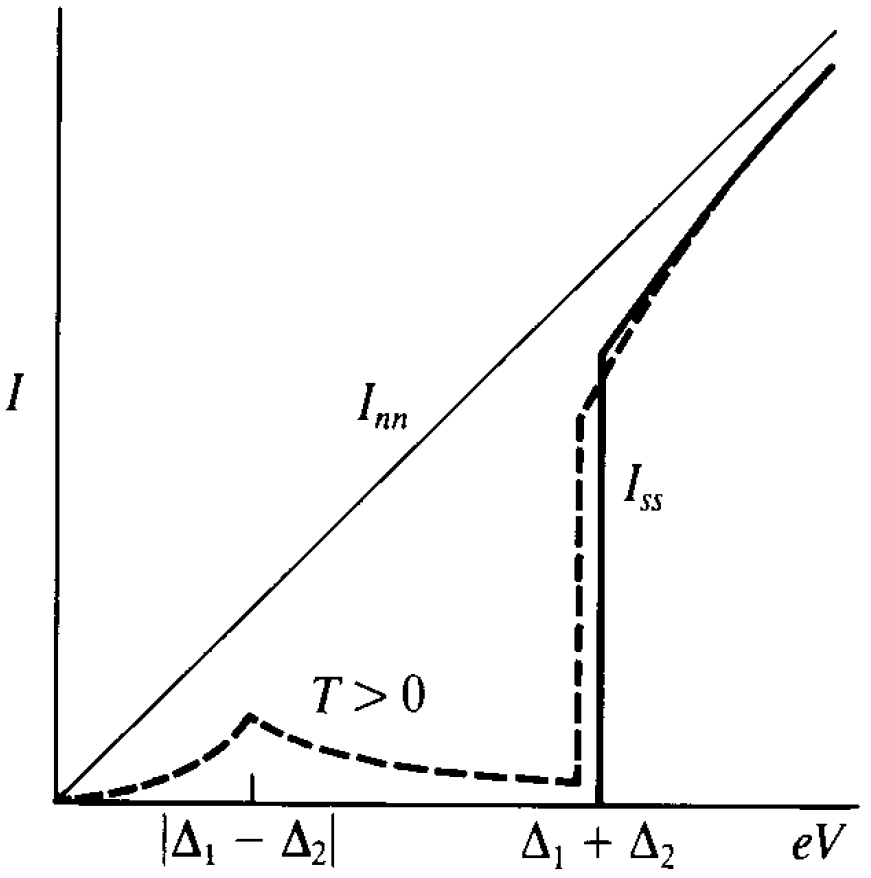
\includegraphics[width=0.45\textwidth]{immagini/IV_SIS.png}
\end{figure}
\hspace{-0.6cm}A temperatura nulla non compare alcuna corrente finché la tensione applicata non raggiunge la somma dei due gap energetici. Questo si comprende osservando il diagramma a bande nel caso $T=0$:
\begin{figure}[H]
    \centering
    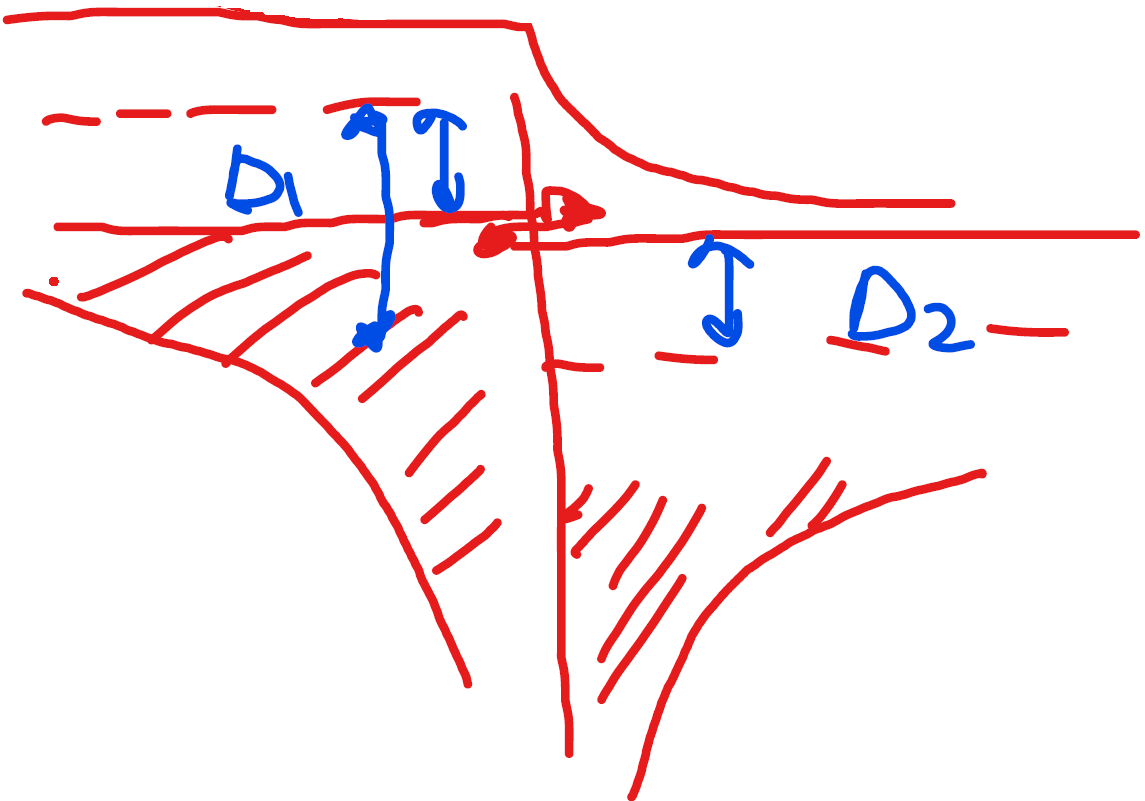
\includegraphics[width=0.4\textwidth]{immagini/SIS_junction_zero_temperature.png}
\end{figure}
\hspace{-0.6cm}Per avere una corrente di tunneling consiste un livello occupato deve poter tunnelare verso un livello disponibile dall'altro lato. Perché ciò avvenga, è necessario che la differenza di potenziale applicata sia tale da allineare opportunamente le bande energetiche, cioè $eV=\Delta_1+\Delta_2$.\\
A temperatura nulla, quindi, la corrente compare soltanto quando la tensione raggiunge la somma dei due gap. In questo caso si osserva un brusco aumento della corrente, perché appena questa condizione viene soddisfatta, gli elettroni di uno dei due superconduttori trovano immediatamente un grande numero di stati di quasiparticella disponibili nell'altro superconduttore.\\
Se invece la temperatura è finita, la corrente di tunneling assume l'andamento rappresentato dalla linea tratteggiata nella figura precedente: compare un comportamento non monotono con un massimo localizzato a un'energia pari alla differenza tra i due gap. Questo comportamento deriva dai differenti processi di tunneling che coinvolgono gli stati occupati termicamente.\\
Se siamo in grado di misurare sperimentalmente la caratteristica corrente--tensione e osserviamo una forma di questo tipo, possiamo ricavare direttamente i due gap $\Delta_1$ e $\Delta_2$. Infatti, il primo massimo della corrente si trova in corrispondenza di $|eV_1|=|\Delta_1-\Delta_2|$, mentre il brusco aumento della corrente si verifica invece per $|eV_2|=|\Delta_1+\Delta_2|$. Dai valori di tensione in cui compaiono questi due fenomeni possiamo quindi determinare i gap dei due superconduttori che formano la giunzione.\\
Vediamo ora qualitativamente perché compare questo comportamento:
\begin{figure}[H]
    \centering
    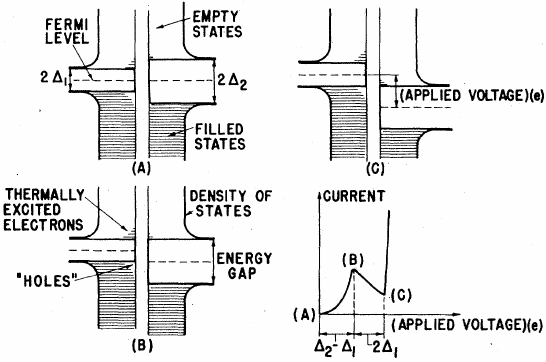
\includegraphics[width=0.9\textwidth]{immagini/SIS_junction_finite_temperature.png}
    %\caption*{Tunneling tra due superconduttori con gap energetici differenti a temperatura maggiore di $0^\circ$ K.     (a) Nessuna tensione applicata tra i due conduttori. (b) Applicando una tensione diventa energeticamente possibile per un numero sempre maggiore di elettroni eccitati termicamente fluire dal superconduttore con gap minore verso quello con gap maggiore. Alla tensione mostrata, tutti gli elettroni eccitati trovano stati disponibili sul lato destro. (c) Aumentando ulteriormente la tensione, non entrano in gioco nuovi elettroni e, poiché diminuisce il numero di stati accessibili per il tunneling, la corrente diminuisce al crescere della tensione. Quando la tensione diventa sufficientemente grande, gli elettroni al di sotto del gap nel superconduttore di sinistra trovano stati vuoti sul lato destro e si osserva un rapido aumento della corrente. (d) Andamento schematico della caratteristica corrente--tensione.}
\end{figure}
\hspace{-0.6cm}Il punto di partenza è la situazione rappresentata in (a). Abbiamo due superconduttori con gap differenti, $\Delta_1$ a sinistra e $\Delta_2$ a destra. I potenziali chimici sono allineati perché non è applicata alcuna tensione.\\
In questa configurazione esistono alcune eccitazioni termiche soltanto nel superconduttore con gap minore, perché nell'altro superconduttore l'energia richiesta per creare eccitazioni è più grande e quindi gli effetti termici risultano molto più piccoli.\\
In tali condizioni possiamo avere soltanto una piccola corrente dovuta a pochi livelli occupati che riescono a tunnelare verso stati disponibili sull'altro lato. Si tratta quindi di un effetto molto debole.\\
Successivamente aumentiamo la tensione applicata, passando alla situazione (b). I due potenziali chimici non risultano più allineati e gli elettroni eccitati termicamente trovano ora livelli energetici disponibili nell'altro superconduttore.\\
Osservando la figura (d), vediamo che la corrente cresce fino a raggiungere un massimo quando $eV = \Delta_1-\Delta_2$.  Questa configurazione corrisponde precisamente al caso illustrato in (b).\mn{Nota di ChatGPT: questo accade perché a questa tensione tutti i livelli occupati sul lato sinistro riescono a trovare stati disponibili sul lato destro, realizzando una sorta di condizione di risonanza. È per questo motivo che compare il massimo della corrente.}\\
Se aumentiamo ulteriormente la tensione, si raggiunge la situazione illustrata in (c). In questo caso i processi di tunneling precedenti non possono più verificarsi efficacemente, perché molti degli stati finali accessibili cadono all'interno del gap energetico dell'altro superconduttore.\\
Di conseguenza esiste una regione di tensioni superiori a $\Delta_1-\Delta_2$ in cui la corrente, invece di aumentare, diminuisce. Le due bande risultano infatti soltanto parzialmente sovrapposte e il numero di stati occupati che riescono a trovare livelli disponibili sull'altro lato si riduce. Questo è l'origine del comportamento non monotono della corrente.\\
Infine, aumentando ancora la tensione, si raggiunge la condizione $eV=\Delta_1+\Delta_2$. In questo caso tutti gli stati eccitati del superconduttore di sinistra trovano stati eccitati disponibili nel superconduttore di destra e si osserva quindi un brusco aumento della corrente.
\subsection{Scattering di Andreev}
Discutiamo ora un altro effetto identificato da Andreev, noto come scattering di Andreev. Nel seguito ne daremo una descrizione qualitativa.\\
Supponiamo di avere un'interfaccia metallo normale--superconduttore, senza alcuna barriera isolante.
\begin{figure}[H]
    \centering
    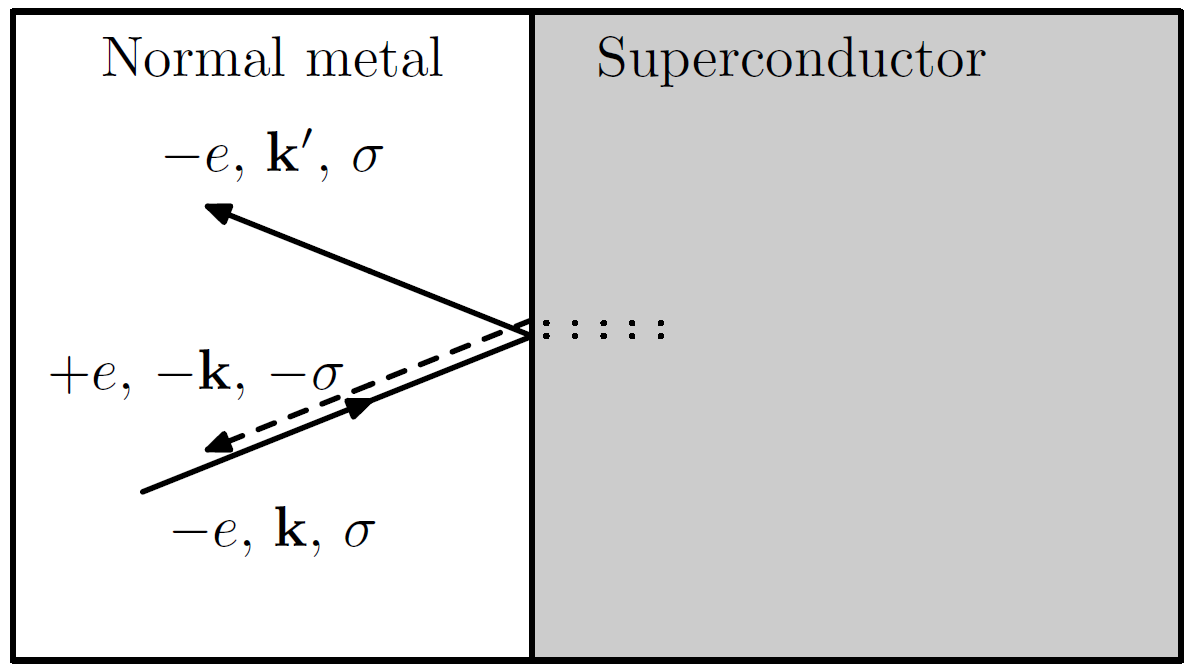
\includegraphics[width=0.4\textwidth]{immagini/Andreev_scattering.png}
\end{figure}
\hspace{-0.6cm}Sul lato sinistro abbiamo elettroni normali, mentre sul lato destro abbiamo coppie di Cooper.\\
Può accadere che un elettrone con carica $-e$, quantità di moto $\vb{k}$ e spin $\sigma$ si propaghi nel metallo normale e raggiunga la superficie del superconduttore. Se il superconduttore si trova nello stato fondamentale BCS, questo elettrone non può partecipare direttamente alla superconduttività, poiché non esistono stati disponibili a singola particella all'interno del gap energetico. In questo caso l'elettrone viene riflesso specularmente: la sua carica rimane invariata, così come il suo spin, mentre la quantità di moto cambia in modo tale da conservare la quantità di moto totale.\\
Esiste tuttavia un altro possibile processo, identificato da Andreev, che consiste nella combinazione dell'elettrone incidente con un secondo elettrone del metallo normale per formare una coppia di Cooper che entra nel superconduttore.\\
In questo caso, nel superconduttore compare una coppia di Cooper aggiuntiva, quindi una carica complessiva pari a $-2e$. Poiché la carica totale deve conservarsi, sul lato normale compare una lacuna (\textit{hole}), cioè una carica negativa mancante, che possiamo interpretare come una buca nel metallo normale.\\
Inoltre, per conservare la quantità di moto, dato che l'elettrone che entra nel superconduttore mantiene la propria quantità di moto, la lacuna riflessa deve avere quantità di moto $-\vb{k}$. Analogamente, per la conservazione dello spin, se l'elettrone entrato nel superconduttore possiede spin $\sigma$, la lacuna risultante deve avere spin opposto $-\sigma$.\\
Dal punto di vista qualitativo possiamo quindi descrivere questo processo come un elettrone incidente che colpisce l'interfaccia e una lacuna riflessa con carica opposta, quantità di moto opposta e spin opposto, che quindi si propaga all'indietro rispetto all'elettrone incidente.\\
Il risultato netto del processo è che due elettroni vengono trasferiti nel superconduttore, mentre sul lato normale avviene un processo equivalente all'annichilazione di un elettrone e alla creazione di una lacuna, il tutto nel rispetto della conservazione della carica.\\
Come si può osservare sperimentalmente questo effetto? Il punto fondamentale è il seguente. Consideriamo il processo di Andreev illustrato in figura:
\begin{figure}[H]
    \centering
    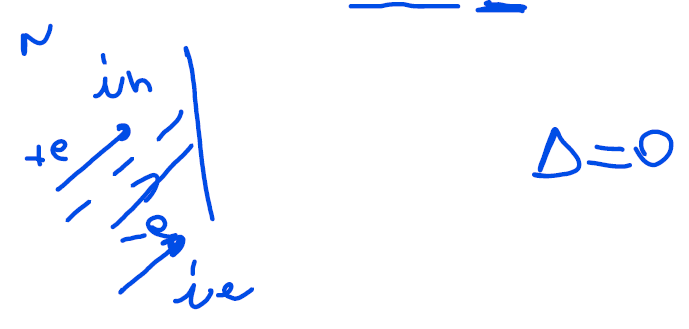
\includegraphics[width=0.4\textwidth]{immagini/Andreev_process.png}
\end{figure}
\hspace{-0.6cm}Nel metallo normale le lacune trasportano carica opposta e si propagano in direzione opposta rispetto all'elettrone incidente. Se quindi abbiamo un elettrone entrante che si muove in una certa direzione, esso produce una corrente in quella direzione; contemporaneamente, una lacuna che si muove nella direzione opposta genera anch'essa una corrente nello stesso verso dell'elettrone incidente.\\
Di conseguenza, questo processo produce una corrente pari al doppio della corrente che si avrebbe nel caso di un metallo normale oppure nel caso di un processo di tunneling ordinario indotto da una tensione sufficientemente grande da superare il gap energetico.\\
L'osservazione sperimentale di una corrente doppia rispetto a quella attesa nel caso $\Delta=0$ costituisce quindi una chiara evidenza dell'esistenza dei processi di Andreev.
\section{Effetto Josephson}
Finora abbiamo visto che cosa accade quando tra un metallo normale e un superconduttore, oppure tra due superconduttori, è presente uno strato isolante. Considerando la densità degli stati dei superconduttori, abbiamo essenzialmente analizzato quali processi possono avere luogo quando il tunneling attraverso la barriera isolante comporta la rottura delle coppie di Cooper.\\
Questo dà origine a particolari relazioni corrente--tensione, caratterizzate tipicamente dalla presenza di intervalli di tensione nei quali non scorre corrente. Il motivo è che il sistema deve fornire energia sufficiente per rompere almeno una o più coppie di Cooper affinché possa comparire una corrente. In questo caso, le singole quasiparticelle tunnelano indipendentemente attraverso la giunzione, poiché provengono dal condensato formato dalle coppie di Cooper.\\
Esiste tuttavia un altro fenomeno possibile, scoperto da Josephson nel 1962, noto come effetto Josephson. Esso consiste nel fatto che, invece di avere singoli elettroni che attraversano la giunzione, sono le coppie di Cooper a ``tunnelare'' attraverso la barriera.\mn{In realtà questa non è la descrizione più corretta del fenomeno. Più precisamente, ciò che avviene è la formazione di un unico condensato coerente modificato che coinvolge entrambi i superconduttori separati dalla barriera isolante.}\\
In questo processo compare una supercorrente, perché non avviene la rottura delle coppie di Cooper, nonostante non sia presente alcuna differenza di potenziale tra i due elettrodi.\\
Dal punto di vista qualitativo, ciò che accade è che la funzione d'onda elettronica penetra attraverso la barriera isolante, dando luogo a un accoppiamento coerente tra i due superconduttori. La descrizione teorica del fenomeno richiede quindi la formazione di uno stato coerente collettivo dell'intero sistema elettronico.\\
Nel seguito vedremo come descrivere quantitativamente questo effetto.
\subsection{Giunzione Josephson}
Consideriamo la giunzione Josephson più semplice che possiamo realizzare. Vedremo che questa non è l'unica possibilità, ma rappresenta la configurazione standard:
\begin{figure}[H]
    \centering
    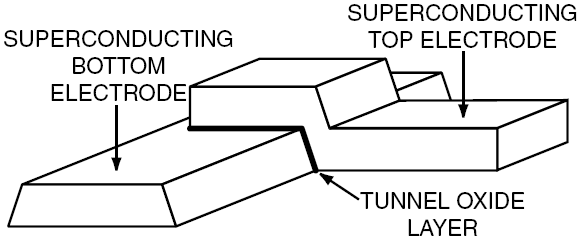
\includegraphics[width=0.5\textwidth]{immagini/Josephson_junction.png}
\end{figure}
\hspace{-0.6cm}Abbiamo due elettrodi superconduttivi, generalmente realizzati uno sopra l'altro. Tra i due strati superconduttivi è presente un ossido che svolge il ruolo di barriera isolante.\\
Tipicamente la giunzione viene realizzata con alluminio e l'ossido è $\rm Al_x O_y$, con $x \leq 2$ e $y \leq 3$. Lo spessore della barriera è soltanto di circa $2$--$3\;\rm nm$, mentre le dimensioni laterali tipiche sono dell'ordine di $0.1\times0.1\;\rm \mu m^2$ per le giunzioni più piccole e $1\times1\;\rm \mu m^2$ per quelle più grandi.\\
Naturalmente, le temperature alle quali questi sistemi operano devono essere tali da mantenere i materiali nello stato superconduttivo; tipicamente si lavora a $T \sim 20$--$30\;\rm mK$, mentre il gap energetico di questi materiali è dell'ordine di $200\;\mu\rm eV$. Il gap è quindi molto maggiore dell'energia termica associata alla temperatura operativa, che vale circa $3\;\mu\rm eV$.\\
Dal punto di vista schematico possiamo rappresentare la giunzione nel modo seguente:
\begin{figure}[H]
    \centering
    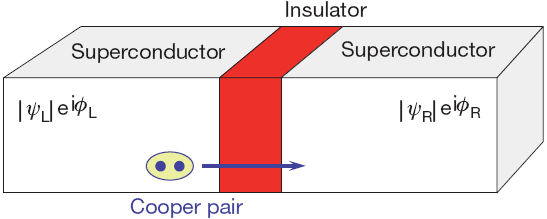
\includegraphics[width=0.5\textwidth]{immagini/Josephson_effect.png}
\end{figure}
\hspace{-0.6cm}Abbiamo dunque due superconduttori separati da uno strato isolante.\\
Supponiamo ora che il sistema si trovi a temperatura nulla. In questo caso, sui due lati della giunzione avremo il condensato superconduttivo, descritto da una funzione d'onda macroscopica per il lead sinistro e per quello destro:
\begin{equation*}
    \psi_{L,R}=|\psi_{L,R}| e^{i\phi_{L,R}}
\end{equation*}
L'interpretazione del modulo di questa funzione è quella della radice quadrata della densità elettronica nei due lati:
\begin{equation*}
    |\psi_{L,R}|=\sqrt{n_{L,R}}
\end{equation*}
Se per un momento dimenticassimo che stiamo descrivendo un condensato macroscopico e interpretassimo $\psi$ come la funzione d'onda di una singola particella, dalla meccanica quantistica sappiamo che esiste una probabilità finita che la funzione d'onda penetri in una regione classicamente proibita, cioè una regione in cui il potenziale è maggiore dell'energia della particella. Questo è precisamente l'effetto tunnel.
\begin{figure}[H]
    \centering
    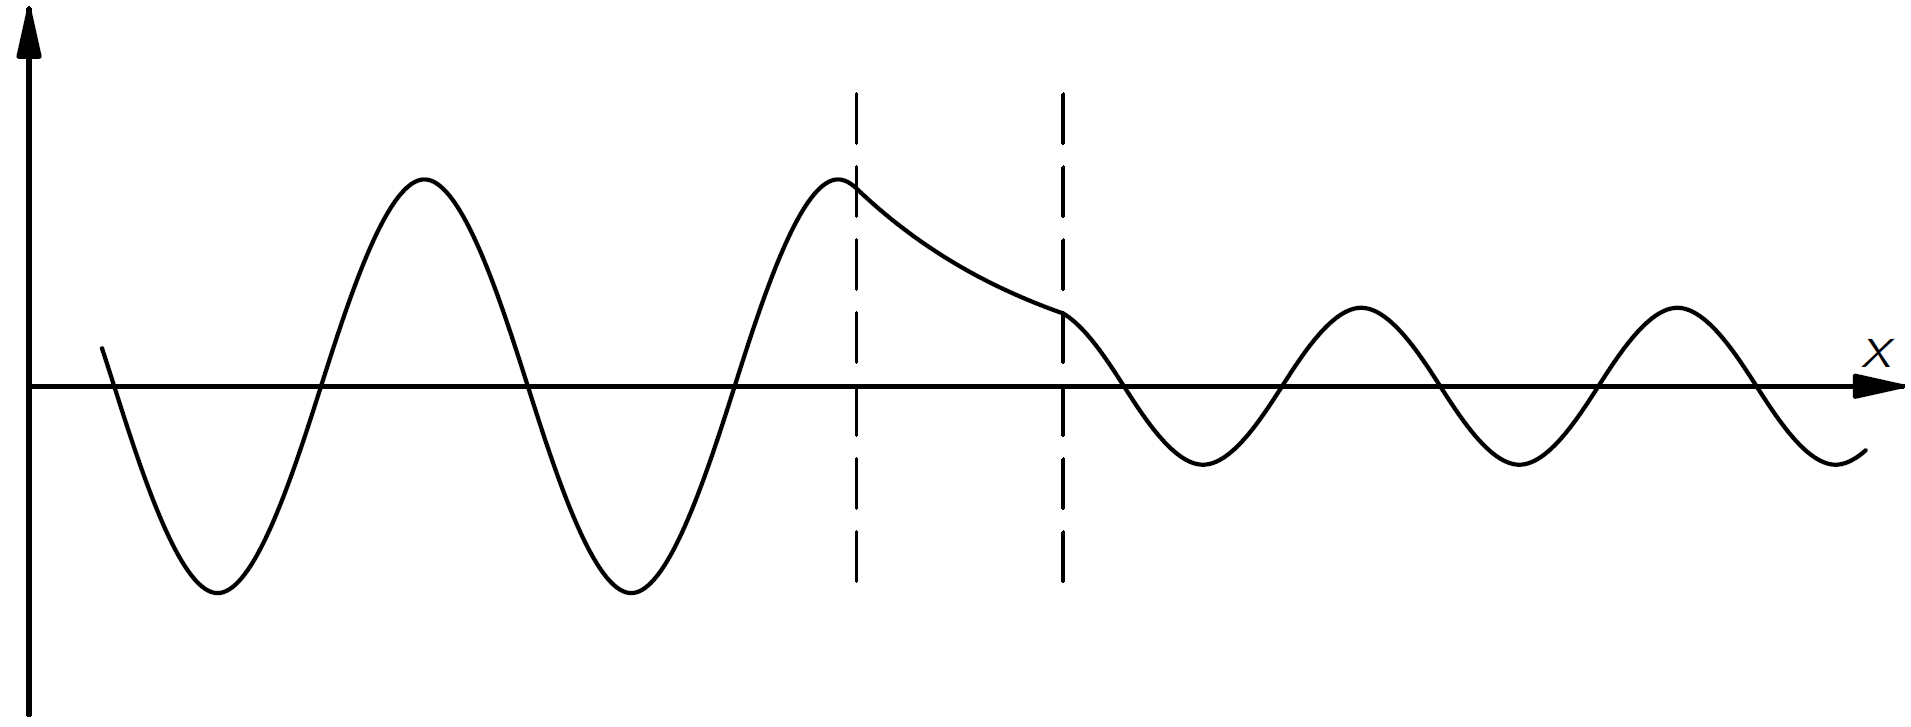
\includegraphics[width=0.6\textwidth]{immagini/tunneling_effect.png}
\end{figure}
\hspace{-0.6cm}Se abbiamo una barriera di tunneling, cioè una barriera in cui l'energia potenziale è maggiore dell'energia della particella, ci aspettiamo che la funzione d'onda penetri all'interno della barriera con un decadimento tipicamente esponenziale. Se la barriera è sufficientemente sottile, la funzione d'onda risulta non nulla anche dall'altro lato, rendendo possibile il tunneling.\\
Lo stesso tipo di descrizione può essere applicato anche al condensato superconduttivo. Possiamo quindi immaginare che la funzione d'onda collettiva del condensato abbia una probabilità non nulla di penetrare nella regione classicamente proibita rappresentata dalla barriera isolante. Questo processo avviene simmetricamente da entrambi i lati, poiché su entrambi i lati della barriera sono presenti superconduttori.\\
In questo senso possiamo interpretare la penetrazione della funzione d'onda macroscopica come un meccanismo di accoppiamento tra i due elettrodi. E, dato che stiamo parlando di un condensato, ciò implica che esiste una probabilità finita di trovare coppie di Cooper provenienti da un lato anche nell'altro lato della giunzione.\\
\mn{Per questa parte mi sono basato su \cite{Feynman}.}
Per descrivere questo effetto possiamo utilizzare una derivazione semplice dell'effetto Josephson, basata sull'idea di trattare il condensato come una funzione d'onda collettiva, ma formalmente descritta come una funzione d'onda a singola particella.\\
Chiamiamo $\psi_L$ l'ampiezza di probabilità di trovare un elettrone sul lato sinistro e $\psi_R$ quella corrispondente al lato destro. Nello stato superconduttivo, $\psi_L$ rappresenta la funzione d'onda collettiva di tutti gli elettroni del lato sinistro, mentre $\psi_R$ descrive analogamente il lato destro.\\
Le due ampiezze devono soddisfare le seguenti equazioni\mn{Le equazioni seguenti non sono altro che le equazioni di Schrödinger per le due funzioni d'onda. Il secondo termine nasce dal fatto che, se immaginiamo che la funzione d'onda superconduttiva possa penetrare attraverso la barriera, allora ciascun lato contiene anche una componente proveniente dall'altro lato.}:
\begin{equation*}
\begin{split}
    i\hbar \pdv{\psi_L}{t}
    &= U_1\psi_L + K\psi_R
    \\
    i\hbar \pdv{\psi_R}{t}
    &= U_2\psi_R + K\psi_L
\end{split}
\end{equation*}
La costante $K$ è una caratteristica della giunzione. Se $K=0$, queste due equazioni descriverebbero semplicemente gli stati fondamentali dei due superconduttori, con energie $U_1$ e $U_2$.\\
L'accoppiamento tra i due lati è invece descritto proprio dal termine proporzionale a $K$, che rappresenta la possibilità di una ``perdita'' di ampiezza di probabilità da un lato all'altro della barriera.\\
Se i due lati fossero identici, avremmo $U_1=U_2$ e potremmo semplicemente eliminare il termine energetico comune. Supponiamo però di collegare i due superconduttori ai terminali di una batteria, in modo da applicare una differenza di potenziale $V$ attraverso la giunzione. In questo caso $U_1-U_2=eV$. Possiamo allora scegliere convenientemente lo zero dell'energia a metà tra i due livelli energetici. Le equazioni diventano quindi:
\begin{equation*}
\begin{split}
    i\hbar \pdv{\psi_L}{t}
    &= \frac{eV}{2}\psi_L + K\psi_R
    \\[0.2cm]
    i\hbar \pdv{\psi_R}{t}
    &= -\frac{eV}{2}\psi_R + K\psi_L
\end{split}
\end{equation*}
Queste sono le equazioni standard di due stati quantistici accoppiati.\\
Per risolverle scriviamo $\psi_L$ e $\psi_R$ in termini di modulo e fase:
\begin{equation*}
    \psi_L
    =
    \sqrt{n_L}e^{i\phi_L}
    \qq{,}
    \psi_R
    =
    \sqrt{n_R}e^{i\phi_R}
\end{equation*}
dove $\phi_L$ e $\phi_R$ sono le fasi dei due superconduttori e $n_L$, $n_R$ rappresentano le densità elettroniche nei due lati della giunzione. In pratica queste densità sono quasi identiche e coincidono essenzialmente con la densità elettronica normale $n_0$ del materiale superconduttore.\\
Sostituendo queste espressioni nelle equazioni precedenti e separando parte reale e parte immaginaria, si ottengono quattro equazioni. Introducendo la differenza di fase $\varphi=\phi_R-\phi_L$, si trova:
\begin{equation}
    \begin{split}
        \dot{n}_L
        &=
        \frac{2}{\hbar}
        K\sqrt{n_Rn_L}
        \sin\varphi
        \\[0.2cm]
        \dot{n}_R
        &=
        -
        \frac{2}{\hbar}
        K\sqrt{n_Rn_L}
        \sin\varphi
    \end{split}
    \label{eq:derivate_densità}
\end{equation}
e
\begin{equation}
    \begin{split}
        \dot{\phi}_L
        &=
        -
        \frac{K}{\hbar}
        \sqrt{\frac{n_R}{n_L}}
        \cos\varphi
        -
        \frac{eV}{2\hbar}
        \\[0.2cm]
        \dot{\phi}_R
        &=
        -
        \frac{K}{\hbar}
        \sqrt{\frac{n_L}{n_R}}
        \cos\varphi
        +
        \frac{eV}{2\hbar}
    \end{split}
    \label{eq:derivate_fasi}
\end{equation}
Consideriamo dapprima le \eqrefcustom{eq:derivate_densità}. Esse mostrano che $\dot{n}_L=-\dot{n}_R$, come è naturale aspettarsi: gli elettroni passano da un lato all'altro, facendo aumentare la densità da un lato e diminuire quella dall'altro.\\
A questo punto si potrebbe osservare che $\dot{n}_L$ e $\dot{n}_R$ dovrebbero essere entrambi nulli se $n_L$ e $n_R$ sono costanti e pari a $n_0$. In realtà queste equazioni non raccontano tutta la fisica del problema. Esse descrivono infatti come le densità inizierebbero a variare se non esistessero forze elettriche aggiuntive dovute allo sbilanciamento tra il fluido elettronico e il background di ioni positivi.\\
Queste equazioni descrivono quindi il tipo di corrente che tenderebbe a instaurarsi. La corrente da sinistra verso destra sarebbe:
\begin{equation*}
    I_s
    =
    2e\mathcal{V}\dot{n}
    =
    2e\mathcal{V}
    \frac{2}{\hbar}
    Kn_0
    \sin\varphi,
\end{equation*}
dove $\mathcal{V}=Ad$ rappresenta il volume della giunzione.\\
Definendo la corrente critica della giunzione come
\begin{equation*}
    I_J
    =
    \frac{4e}{\hbar}
    Kn_0\mathcal{V}
\end{equation*}
la corrente può essere scritta nella forma
\begin{equation}
    I_s
    =
    I_J\sin\varphi.
    \label{eq:current_phase_relation}
\end{equation}
$I_J$ è un parametro caratteristico della giunzione e rappresenta chiaramente il valore massimo della supercorrente, ottenuto per differenze di fase pari a $\pi/2$ o suoi multipli.\\
Una corrente di questo tipo tenderebbe rapidamente a caricare il lato destro della giunzione, se non fosse che i due elettrodi sono collegati ai terminali della batteria. Le correnti provenienti dalla batteria compensano infatti questo trasferimento di carica, mantenendo costanti i potenziali e quindi anche le densità $n_L$ e $n_R$.\\
Le seconde equazioni, \eqrefcustom{eq:derivate_fasi}, descrivono invece l'evoluzione temporale delle fasi $\phi_L$ e $\phi_R$. A differenza delle precedenti, esse dipendono esplicitamente dalla tensione applicata.\\
Siamo interessati soprattutto alla differenza di fase $\varphi=\phi_R-\phi_L$, poiché è questa quantità che compare nella relazione corrente--fase. Sottraendo le due equazioni per $\dot{\phi}_L$ e $\dot{\phi}_R$ otteniamo:
\begin{equation}
    \dot{\varphi}=\frac{eV}{\hbar}
    \label{eq:phase_voltage_relation}
\end{equation}
Questa relazione mostra che, se è presente una differenza di potenziale, allora la differenza di fase tra i due superconduttori evolve nel tempo.\\
L'\eqrefcustom{eq:current_phase_relation} e l'\eqrefcustom{eq:phase_voltage_relation} sono le cosiddette \emph{relazioni di Josephson}. La prima descrive una corrente priva di dissipazione che attraversa la giunzione semplicemente a causa della differenza di fase tra i due superconduttori. La seconda mostra invece che, se la giunzione è inserita in un circuito con una tensione applicata, allora la differenza di fase evolve nel tempo.\\
Nel caso $V=0$, la differenza di fase resta costante e quindi anche la supercorrente rimane costante nel tempo. Se invece è presente una tensione costante $V=V_0\neq0$, allora la differenza di fase evolve linearmente:
\begin{equation*}
    \varphi(t)=\varphi(0)+\frac{2eV_0}{\hbar}t
\end{equation*}
Di conseguenza, anche la corrente diventa una funzione oscillante del tempo.\\
In pratica, però, tali oscillazioni sono estremamente rapide. Per questo motivo, sperimentalmente si parla ancora di effetto Josephson in corrente continua (DC Josephson effect), poiché ciò che viene effettivamente misurato è spesso la corrente mediata nel tempo, che risulta costante e inferiore alla supercorrente ideale che si avrebbe con fase perfettamente costante.\\
In precedenza abbiamo menzionato l'effetto Josephson parlando della rottura spontanea della simmetria di gauge. Abbiamo osservato che questa situazione è analoga alla transizione ferromagnetica: un materiale paramagnetico sviluppa spontaneamente una magnetizzazione lungo una direzione arbitraria, rompendo la simmetria del sistema.\\
Per rivelare la direzione della magnetizzazione non basta osservare un singolo campione isolato; è invece necessario mettere in interazione due materiali ferromagnetici, in modo che la loro interazione magnetica renda osservabile tale direzione privilegiata.\\
La stessa idea vale per la superconduttività. La rottura spontanea della simmetria di gauge implica che ciascun superconduttore possieda una fase macroscopica ben definita. Questa fase, però, diventa fisicamente osservabile soltanto quando mettiamo due superconduttori in contatto attraverso una giunzione Josephson.\\
In questo caso, la differenza tra le due fasi produce direttamente una supercorrente attraverso la giunzione. L'effetto Josephson rappresenta quindi anche una manifestazione sperimentale della rottura spontanea della simmetria di gauge nel superconduttore.
\subsection{Realizzazioni delle giunzioni Josephson}
Come realizziamo una giunzione Josephson?
\begin{figure}[H]
    \centering
    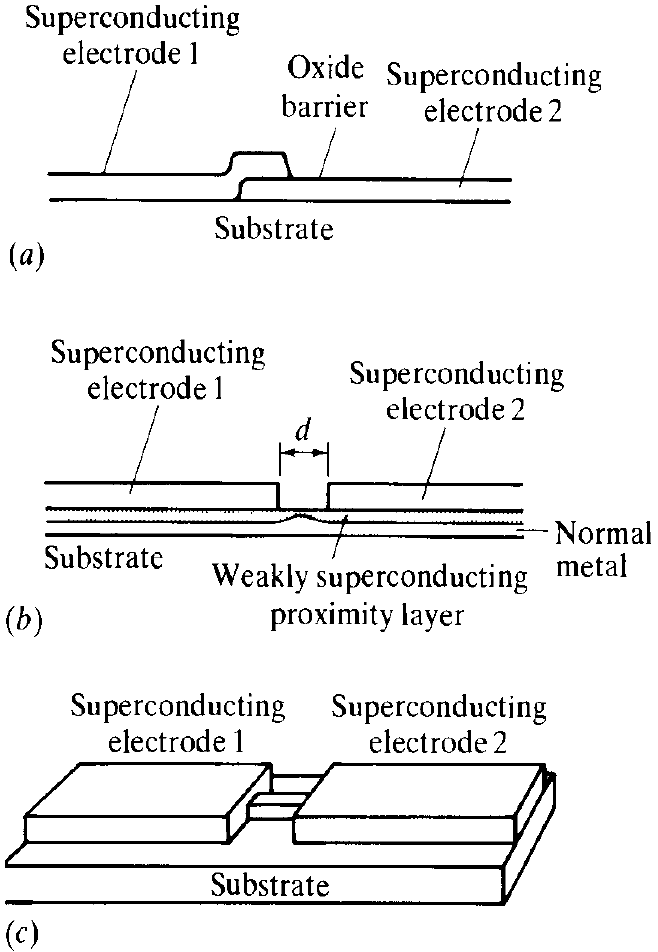
\includegraphics[width=0.5\textwidth]{immagini/Josephson_junction_realization.png}
\end{figure}
\hspace{-0.6cm}Quello che abbiamo menzionato finora è il caso (a), cioè il più semplice: uno strato di ossido cresciuto naturalmente tra due superconduttori, tipicamente in una struttura perpendicolare. Questa configurazione prende il nome di giunzione SIS (\textit{superconducting--insulating--superconducting}).\\
Esistono però anche altri modi per ottenere una giunzione Josephson. In particolare, possiamo avere effetto Josephson, cioè una supercorrente che fluisce, anche in assenza di un materiale isolante tra i due superconduttori.\\
Possiamo infatti realizzare una giunzione superconducting--normal--superconducting, come nel caso (b). In questo caso non abbiamo un materiale isolante, ma uno spazio tra i due superconduttori, depositati sopra un substrato che diventa debolmente superconduttivo attraverso il cosiddetto \emph{effetto di prossimità}.\\
L'effetto di prossimità consiste nel fatto che un materiale normale può acquisire proprietà superconduttive per il semplice fatto di trovarsi a contatto con un superconduttore; almeno una piccola regione del metallo normale diventa quindi anch'essa superconduttiva.\\
In questa configurazione, sui due lati è presente una funzione d'onda superconduttiva, e la possibilità di avere una supercorrente che attraversa la giunzione è legata proprio alla presenza dello strato sottostante che diventa debolmente superconduttivo. Ciò che accade è che le coppie di Cooper possono diffondere nel metallo prossimitizzato, dando origine a una supercorrente attraverso la giunzione.\\
Una situazione simile si verifica quando, al posto di un metallo normale prossimitizzato, abbiamo uno strato di grafene. Questo è il caso della giunzione Josephson planare, nella quale i due elettrodi superconduttivi sono separati da uno strato di grafene.
\begin{figure}[H]
    \centering
    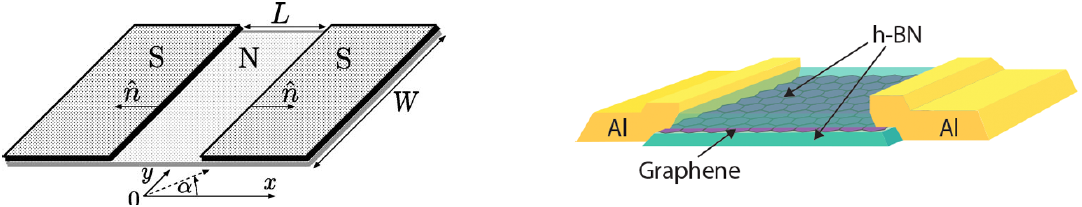
\includegraphics[width=0.8\textwidth]{immagini/graphene_Josephson_junction.png}
\end{figure}
\hspace{-0.6cm}Sperimentalmente il sistema appare come nella figura sopra. Lo strato di grafene è collegato ai lead superconduttivi e il contatto risulta quasi unidimensionale, poiché il grafene tocca gli elettrodi lungo una linea.\\
Inoltre il grafene deve essere sufficientemente isolato dall'ambiente; per questo motivo si utilizza spesso nitruro di boro esagonale (\textit{hexagonal boron nitride}, hBN), che presenta un eccellente accoppiamento strutturale con il grafene e introduce pochissime disomogeneità.\\
In definitiva, abbiamo un materiale normale oppure uno strato di grafene collegato a due superconduttori. Anche in questo caso otteniamo una giunzione Josephson, concettualmente non molto diversa dai casi precedenti.\\
Queste giunzioni Josephson presentano però una relazione corrente--fase che non coincide con la semplice dipendenza sinusoidale derivata in precedenza. Essa è rappresentata schematicamente nella figura seguente:
\begin{figure}[H]
    \centering
    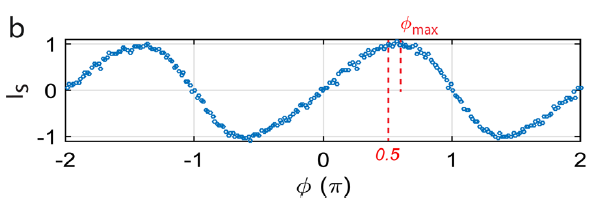
\includegraphics[width=0.6\textwidth]{immagini/current_phase_relation_graphene.png}
\end{figure}
\hspace{-0.6cm}La relazione rimane periodica, ma non è perfettamente sinusoidale e presenta una certa asimmetria. Inoltre, tale relazione corrente--fase può essere modulata tramite un gate: variando il potenziale di gate collegato ai due superconduttori, cambia infatti la forma della relazione corrente--fase.\\
Un'altra possibilità di ottenere l'effetto Josephson è il caso (c), detto \emph{weak link} oppure giunzione superconducting--constriction--superconducting.\\
In questo caso abbiamo un materiale interamente superconduttivo, ma con una strozzatura molto stretta tra le due regioni. Non è presente né uno strato isolante né uno spazio vuoto; tuttavia la regione di costrizione è così piccola da produrre un fenomeno analogo al tunneling, come se fosse presente una barriera isolante. Anche in questo caso compare quindi una corrente Josephson.\\
Abbiamo derivato in maniera fenomenologica le relazioni che caratterizzano la giunzione Josephson. Questa giunzione costituisce l'elemento circuitale fondamentale dei circuiti superconduttivi, oggi utilizzati in numerose applicazioni, ad esempio nei magnetometri.\\
Per studiare come l'effetto Josephson entri in gioco in circuiti contenenti giunzioni Josephson, si utilizza un modello elettrico in cui l'elemento superconduttivo viene interrotto dalla giunzione stessa.\\
Nei circuiti, la giunzione Josephson viene rappresentata convenzionalmente con una croce oppure con una croce racchiusa in un piccolo riquadro: questo è il simbolo circuitale della giunzione Josephson.\\
Per descrivere realisticamente questo elemento dobbiamo però considerare che la giunzione è costituita da due elettrodi posti uno di fronte all'altro e separati da uno strato isolante. Di conseguenza, i due elettrodi formano naturalmente anche un condensatore.\\
Per includere correttamente la giunzione all'interno di un circuito è quindi necessario tenere conto anche della capacità associata alla struttura.\\
Inoltre dobbiamo ricordare che non esiste soltanto il condensato superconduttivo. Finora abbiamo considerato soltanto lo stato fondamentale, cioè il condensato, ma sappiamo che esistono anche stati eccitati.\\
Questi stati eccitati diventano rilevanti a temperatura finita, quando possono verificarsi processi di tunneling a singola particella. In tali condizioni il comportamento della giunzione può diventare resistivo.\\
Quando il sistema entra in regime resistivo, il comportamento dipende dalla tensione applicata. Ricordiamo infatti che, nella caratteristica corrente--tensione di un superconduttore, non si osserva corrente fino al raggiungimento del gap $\Delta$; successivamente la corrente cresce e, per tensioni sufficientemente elevate, il sistema mostra un comportamento resistivo.\\
Questo significa che, per descrivere in generale una giunzione Josephson in un circuito, dobbiamo includere anche la possibilità di un canale resistivo che si attiva quando la tensione supera un certo valore. Si tratta quindi di una resistenza dipendente dalla tensione applicata.\\
Un modello circuitale che include tutti questi effetti è rappresentato schematicamente nella figura seguente:
\begin{figure}[H]
    \centering
    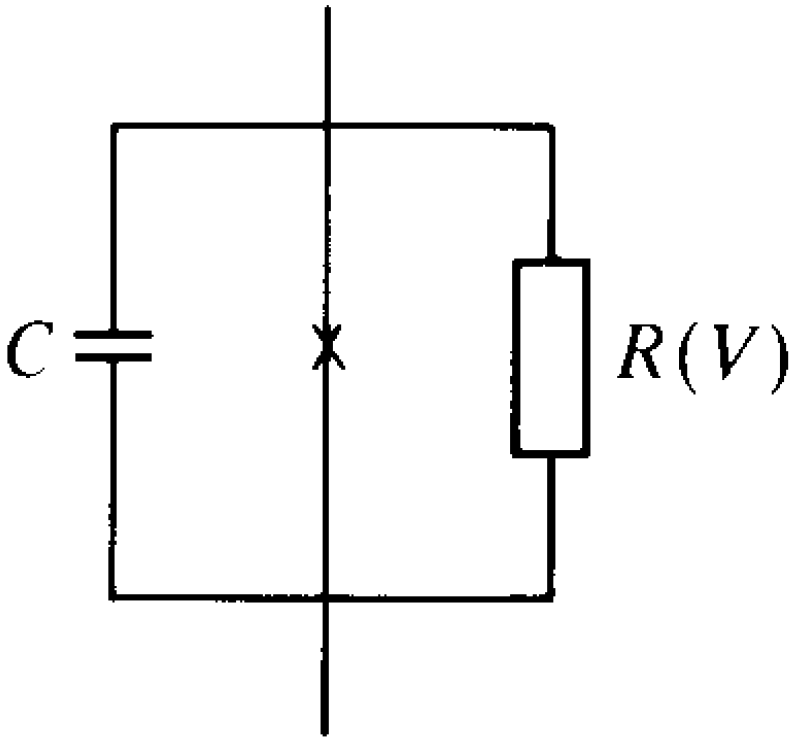
\includegraphics[width=0.3\textwidth]{immagini/RC_Josephson_junction.png}
\end{figure}
\hspace{-0.6cm}In questo modo si realizza il cosiddetto modello \emph{resistively and capacitively shunted Josephson junction} (RCSJ), cioè una giunzione Josephson con due shunt: uno capacitivo e uno resistivo.\\
Vedremo ora come questo elemento circuitale entra in gioco e come debba essere analizzato.
\subsection{Differenza di fase gauge-invariante e relazioni di Josephson in forma gauge-invariante}
Prima di passare oltre, consideriamo che cosa accade in presenza di un campo magnetico, poiché la descrizione sviluppata finora vale nel caso in cui il campo magnetico sia assente.\\
In presenza di un campo magnetico, dobbiamo scrivere relazioni gauge-invarianti. Sappiamo infatti che, se è presente un campo magnetico, dobbiamo effettuare una trasformazione di gauge, che implica una modifica del potenziale scalare e del potenziale vettore nel modo seguente:
\begin{equation*}
    \begin{dcases}
        V \to V - \frac{1}{c} \pdv{\Lambda}{t}
        \\[0.2cm]
        \vb{A} \to \vb{A} + \grad{\Lambda}
    \end{dcases}
\end{equation*}
Abbiamo inoltre visto che, affinché la teoria resti gauge-invariante, anche la funzione d'onda del condensato deve trasformarsi mediante un fattore di fase dipendente dalla carica e dalla funzione di gauge $\Lambda$:
\begin{equation*}
    \psi \to \psi e^{i \frac{2e}{\hbar c} \Lambda}
\end{equation*}
Questo implica che la densità di supercorrente assuma la forma
\begin{equation*}
    \vb{J}_s
    =n_s 2e \vb{v}_s
    =\frac{2e}{m}\qty(\hbar \grad{\varphi} - \frac{2e}{c}\vb{A}) \abs{\psi}^2
\end{equation*}
A partire da questa espressione possiamo definire la differenza di fase gauge-invariante $\gamma$ tra i due superconduttori:
\begin{equation*}
    \gamma
    =
    \int_{1}^{2}
    \grad{\varphi}\vdot d\vb{s}
    -
    \frac{2e}{\hbar c}
    \int_{1}^{2}
    \vb{A}\vdot d\vb{s}
\end{equation*}
dove gli estremi di integrazione indicano che l'integrale viene calcolato da un elettrodo all'altro della giunzione.\\
Il termine gauge-invariante è quindi composto da due contributi: il primo coincide con quello che compare in assenza di campo magnetico, mentre il secondo è l'integrale del potenziale vettore tra i due lati della giunzione.\\
Possiamo scrivere questa espressione in forma più compatta introducendo il quanto di flusso $\Phi_0=\frac{hc}{2e}$. Inoltre, integrando il primo termine, che è il gradiente della fase, otteniamo
\begin{equation*}
    \gamma
    =
    \Delta\varphi
    -
    \frac{2\pi}{\Phi_0}
    \int_{1}^{2}
    \vb{A}\vdot d\vb{s}
\end{equation*}
Questo significa che, se una giunzione Josephson è immersa in un campo magnetico, al posto della semplice differenza di fase $\Delta\varphi$ nell'argomento della funzione seno compare la differenza di fase gauge-invariante $\gamma$.\\
In altre parole, la differenza di fase effettiva non è più soltanto quella presente in assenza di campo magnetico, ma include anche un contributo legato al potenziale vettore e quindi al campo magnetico applicato.\\
Le relazioni di Josephson in forma gauge-invariante diventano quindi
\begin{equation*}
    I_s
    =I_J \sin{\gamma}
    \qq{,}
    \pdv{\Delta\varphi}{t}
    =\frac{2e}{\hbar}V
\end{equation*}
\subsection{Quantizzazione del flusso nella teoria BCS}
\textbf{Anello superconduttivo (come nella teoria GL)}\\
Vogliamo ora capire che cosa accade quando una giunzione viene inserita in un circuito e, in particolare, quando uno o due giunzioni interrompono un anello superconduttivo.\\
Già utilizzando la teoria di Ginzburg--Landau abbiamo derivato nel caso di un anello superconduttivo una relazione tra la supercorrente e il flusso del campo magnetico, ed è proprio in quel contesto che abbiamo introdotto il quanto di flusso. Vedremo ora che cosa accade quando l'anello superconduttivo viene interrotto da una o da due giunzioni Josephson, e vedremo che questo permette anche di identificare alcuni dispositivi fisici importanti.\\
Richiamiamo brevemente quanto già visto, riformulandolo però nel linguaggio della teoria BCS. Consideriamo un anello superconduttivo immerso in un campo magnetico applicato perpendicolarmente al piano dell'anello.
\begin{figure}[H]
    \centering
    
\begin{tikzpicture}
        \draw[gray!30!,line width=0.5cm] (0,0) circle (1.6cm);
        \draw (0,0) circle (0.4cm);
        \draw[rotate=45] (-0.4,0) -- (0.4,0);
        \draw[rotate=-45] (-0.4,0) -- (0.4,0);
    \end{tikzpicture}
\end{figure}
\hspace{-0.6cm}Sappiamo che lo stato fondamentale BCS può essere scritto nella forma
\begin{equation*}
    \Psi(\vb{r})
    =
    n_s(\vb{r}) e^{i \varphi(\vb{r})}
\end{equation*}
e che la densità di supercorrente gauge-invariante nell'anello è data da
\begin{equation*}
    \vb{J}_s
    \propto
    \grad{\varphi(\vb{r})}
    -
    \frac{2e}{\hbar c}\vb{A}(\vb{r}).
\end{equation*}
Ricordiamo che questa corrente, come avviene in ogni superconduttore, scorre soltanto in prossimità della superficie del materiale. A causa dell'effetto Meissner, infatti, nel bulk del superconduttore non è presente alcuna supercorrente.\\
Questo significa che, se invece di considerare la superficie guardiamo una linea chiusa sufficientemente interna al materiale, avremo
\[
\vb{J}_s=0.
\]
Di conseguenza, la combinazione presente nella parentesi deve annullarsi. Integrando lungo una linea chiusa interna al superconduttore otteniamo quindi
\begin{equation*}
    \oint
    \grad{\varphi}\vdot\dd{\vb{s}}
    =
    \frac{2e}{\hbar c}
    \oint
    \vb{A}\vdot\dd{\vb{s}}.
\end{equation*}
Consideriamo ora separatamente i due termini.\\
Per il primo termine, l'integrale del gradiente della fase lungo una linea chiusa è necessariamente un multiplo intero di $2\pi$, poiché la fase è una quantità periodica:
\begin{equation*}
    \oint
    \grad{\varphi}\vdot\dd{\vb{s}}
    =
    2\pi n.
\end{equation*}
Questo numero intero rappresenta il numero di avvolgimenti (\textit{winding number}) della fase lungo il percorso chiuso.\\
Per quanto riguarda invece l'integrale del potenziale vettore, dall'elettromagnetismo sappiamo che
\begin{equation*}
    \oint
    \vb{A}\vdot\dd{\vb{s}}
    =
    \int_{\Sigma}
    \vb{B}\vdot\dd{\vb{S}}
    =
    \Phi,
\end{equation*}
dove $\Phi$ è il flusso del campo magnetico attraverso la superficie $\Sigma$ delimitata dal contorno scelto.\\
Combinando le due relazioni otteniamo
\begin{equation*}
    2\pi n
    =
    \frac{2e}{\hbar c}\Phi.
\end{equation*}
Questa relazione implica la quantizzazione del flusso magnetico:
\begin{equation*}
    \Phi
    =
    n\Phi_0,
\end{equation*}
dove
\[
\Phi_0=\frac{hc}{2e}
\]
è il quanto di flusso.\\
Abbiamo già ottenuto questo risultato nella teoria di Ginzburg--Landau; qui lo stiamo semplicemente riformulando a partire dall'espressione della supercorrente in termini della fase del condensato BCS.\\
Questa relazione implica che, se prendiamo un anello metallico in presenza di un campo magnetico esterno e lo raffreddiamo al di sotto della temperatura critica, il campo magnetico viene espulso dal materiale a causa dell'effetto Meissner. Tuttavia, il flusso magnetico rimane intrappolato nell'anello in quantità discrete, multiple del quanto di flusso.\\
Questo flusso viene mantenuto dalla presenza di una supercorrente che circola lungo la superficie dell'anello.\\[0.2cm]
\textbf{Anello superconduttivo interrotto da una giunzione Josephson}\\
Supponiamo ora di interrompere l'anello mediante una giunzione Josephson.
\begin{figure}[H]
    \centering
    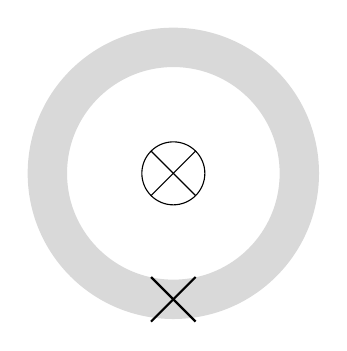
\begin{tikzpicture}
        \draw[gray!30!,line width=0.5cm] (0,0) circle (1.6cm);
        \draw (0,0) circle (0.4cm);
        \draw[rotate=45] (-0.4,0) -- (0.4,0);
        \draw[rotate=-45] (-0.4,0) -- (0.4,0);

        % giunzione
        \begin{scope}[shift={(0,-1.6)},rotate=90]
            \draw[thick, rotate=45] (-0.4,0) -- (0.4,0);
            \draw[thick, rotate=-45] (-0.4,0) -- (0.4,0);
        \end{scope}
    \end{tikzpicture}
\end{figure}
\hspace{-0.6cm}Tutto ciò che abbiamo detto finora continua a valere: in presenza di un campo magnetico la supercorrente deve essere gauge-invariante e, nel bulk del materiale superconduttivo, la corrente deve annullarsi. Quindi ancora una volta abbiamo $\vb{J}_s=0$.\\
La differenza rispetto al caso precedente è che ora il percorso chiuso non attraversa soltanto il superconduttore, ma contiene anche la giunzione Josephson. Di conseguenza, l'integrale del gradiente della fase lungo il contorno si separa in due contributi:
\begin{equation*}
    2\pi n
    =\oint \grad{\varphi}\vdot\dd{\vb{s}}
    =\int_{\text{sc}} \grad{\varphi}\vdot\dd{\vb{s}} + \int_{1}^{2} \grad{\varphi}\vdot\dd{\vb{s}}
\end{equation*}
Il secondo termine non è altro che la differenza di fase ai capi della giunzione, $\Delta\varphi = \phi_R-\phi_L$; il primo termine, essendo valutato all'interno del superconduttore, può invece essere espresso tramite il potenziale vettore:
\begin{equation*}
    \int_{\text{sc}}
    \grad{\varphi}\vdot\dd{\vb{s}}
    =
    \frac{2e}{\hbar c}
    \int_{\text{sc}}
    \vb{A}\vdot\dd{\vb{s}}.
\end{equation*}
Poiché il percorso differisce dal contorno chiuso completo soltanto nella piccola regione occupata dalla giunzione, possiamo approssimare questo integrale con quello sull'intero contorno chiuso.\mn{In pratica stiamo trascurando il contributo della giunzione.}
Otteniamo quindi
\begin{equation*}
    \frac{2e}{\hbar c}
    \int_{\text{sc}}
    \vb{A}\vdot\dd{\vb{s}}
    \approx
    \frac{2e}{\hbar c}\Phi
    =
    2\pi\frac{\Phi}{\Phi_0}
\end{equation*}
Complessivamente si ha quindi
\begin{equation*}
    2\pi n
    =
    \Delta\varphi
    +
    2\pi\frac{\Phi}{\Phi_0}
\end{equation*}
Scegliendo $n=0$,\mn{Il motivo di questa scelta è da chiarire meglio.} otteniamo
\begin{equation*}
    \Delta\varphi=-2\pi\frac{\Phi}{\Phi_0}
\end{equation*}
Questo significa che la differenza di fase ai capi della giunzione è direttamente proporzionale al flusso magnetico concatenato con l'anello.\\
Di conseguenza, se abbiamo una giunzione Josephson che interrompe un anello superconduttivo immerso in un campo magnetico, esiste una quantità osservabile macroscopicamente, cioè il flusso magnetico, direttamente proporzionale alla differenza di fase del condensato tra i due lati della giunzione.\\
In altre parole, la relazione precedente collega la differenza di fase della funzione d'onda superconduttiva — una quantità microscopica, profondamente legata alla natura dello stato superconduttivo e difficilmente osservabile direttamente — a una grandezza macroscopica facilmente misurabile, cioè il flusso magnetico attraverso l'anello, che può essere realizzato con dimensioni arbitrarie.
\subsection{Dispositivo a interferenza quantistica superconduttiva (SQUID)}
Se modifichiamo leggermente il circuito e, invece di avere una singola giunzione, introduciamo due giunzioni che interrompono il materiale superconduttivo, realizziamo quello che viene chiamato \emph{superconducting quantum interference device} (SQUID), cioè un dispositivo che permette di osservare l'interferenza quantistica tra le funzioni d'onda dei condensati superconduttivi nei due rami del circuito.\\
Facciamo attenzione al significato dell'espressione ``interferenza quantistica''. In meccanica quantistica siamo abituati a parlare di interferenza a partire dalle particelle elementari, poiché descriviamo gli elettroni tramite funzioni d'onda e consideriamo la loro sovrapposizione. Normalmente questo non ci sorprende troppo, perché stiamo parlando di sistemi microscopici.\\
Nel caso dello SQUID, invece, abbiamo un dispositivo che permette di osservare sperimentalmente l'interferenza tra funzioni d'onda di condensati macroscopici. Si tratta quindi di un effetto quantistico che coinvolge funzioni d'onda collettive di un condensato elettronico e che diventa direttamente osservabile attraverso correnti macroscopiche.\\
Vediamo ora come funziona il dispositivo.
\begin{figure}[H]
    \centering
    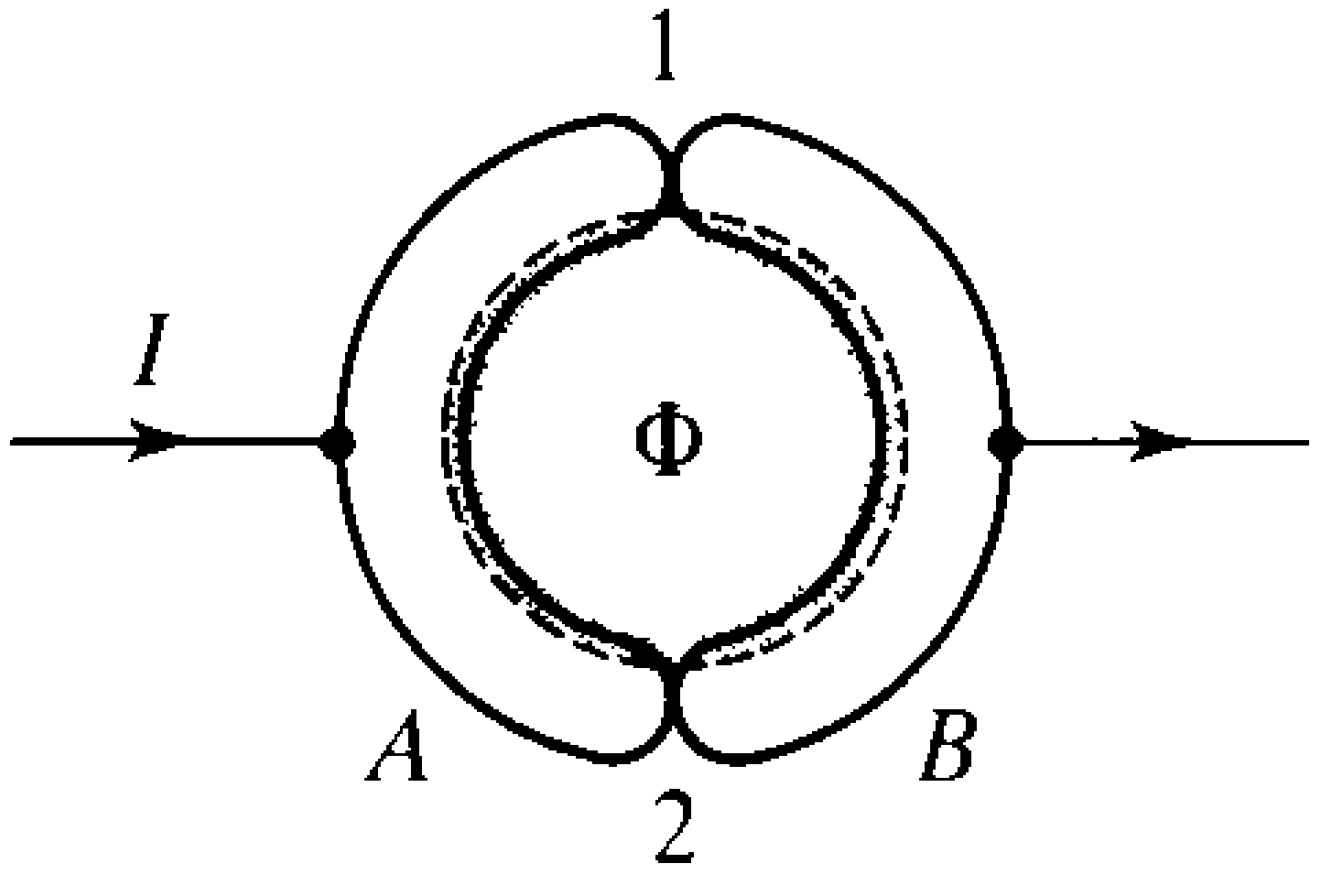
\includegraphics[width=0.45\textwidth]{immagini/SQUID.png}
\end{figure}
\hspace{-0.6cm}Possiamo eseguire per le due giunzioni la stessa derivazione fatta in precedenza nel caso di una singola giunzione. Possiamo quindi definire le due differenze di fase gauge-invarianti:
\begin{equation*}
    \begin{split}
        \gamma_1
        &=
        \Delta\varphi_1
        -
        \frac{2\pi}{\Phi_0}
        \int_{\text{link }1}
        \vb{A}\vdot\dd{\vb{s}}
        \\[0.2cm]
        \gamma_2
        &=
        \Delta\varphi_2
        -
        \frac{2\pi}{\Phi_0}
        \int_{\text{link }2}
        \vb{A}\vdot\dd{\vb{s}}.
    \end{split}
\end{equation*}
Sappiamo inoltre che l'integrale del gradiente della fase lungo un contorno chiuso , poiché questa deve essere una funzione a un sol valore, deve essere nullo a meno di multipli interi di $2\pi$. Possiamo separare tale integrale in un contributo sugli elettrodi e in due contributi corrispondenti alle due giunzioni:
\begin{equation*}
    \oint
    \grad{\varphi}\vdot\dd{\vb{s}}
    =
    \int_{\text{el}}
    \grad{\varphi}\vdot\dd{\vb{s}}
    +
    \int_{\text{link }1}
    \grad{\varphi}\vdot\dd{\vb{s}}
    +
    \int_{\text{link }2}
    \grad{\varphi}\vdot\dd{\vb{s}}.
\end{equation*}
Poiché\mn{Si presti attenzione che le fasi sono definite andando da sinistra verso destra. Se il cammino di integrazione è scelto in senso orario, nel tratto lungo la giunzione 2 ci si sta spostando da destra verso sinistra, il che comporto un segno negativo.}
\begin{equation*}
    \int_{\text{link }1} \grad{\varphi}\vdot\dd{\vb{s}}
    =\Delta\varphi_1
    \qq{,}
    \int_{\text{link }2} \grad{\varphi}\vdot\dd{\vb{s}}
    =-\Delta\varphi_2
\end{equation*}
otteniamo
\begin{equation}
    \Delta\varphi_1
    - \Delta\varphi_2
    + \int_{\text{el}} \grad{\varphi}\vdot\dd{\vb{s}}
    =0
    \quad (\text{mod }2\pi)
    \label{eq:phase_difference_squid}
\end{equation}
Se gli elettrodi sono sufficientemente spessi rispetto alla profondità di penetrazione di London, possiamo assumere che all'interno del bulk superconduttivo la supercorrente sia nulla: $\vb{J}_s = 0$. In questa regione vale quindi
\begin{equation*}
    \grad{\varphi}=\frac{2\pi}{\Phi_0}\vb{A}
\end{equation*}
Possiamo quindi scrivere
\begin{equation*}
    \int_{\text{el}} \grad{\varphi}\vdot\dd{\vb{s}}
    =\frac{2\pi}{\Phi_0}\int_{\text{el}} \vb{A}\vdot\dd{\vb{s}}
\end{equation*}
D'altra parte, possiamo scrivere\mn{Anche in questo passaggio, il termine relativo alla seconda giunzione ha il segno invertito a causa del verso di percorrenza.}
\begin{equation*}
    \begin{split}
        \frac{2\pi}{\Phi_0}\int_{\text{el}} \vb{A}\vdot\dd{\vb{s}}
        & =
        \frac{2\pi}{\Phi_0} \qty( \oint \vb{A}\vdot\dd{\vb{s}}
        - \int_{\text{link }1} \vb{A}\vdot\dd{\vb{s}}
        + \int_{\text{link }2} \vb{A}\vdot\dd{\vb{s}} )
        \\[0.2cm]
        & =
        2\pi \frac{\Phi}{\Phi_0} 
        + \frac{2\pi}{\Phi_0} \qty(
        - \int_{\text{link }1} \vb{A}\vdot\dd{\vb{s}}
        + \int_{\text{link }2} \vb{A}\vdot\dd{\vb{s}} )
    \end{split}
\end{equation*}
Possiamo allora scrivere l'\eqrefcustom{eq:phase_difference_squid}, raggruppando i termini in maniera opportuna, nella forma
\begin{equation*}
    \Delta\varphi_1
    - \int_{\text{link }1} \vb{A}\vdot\dd{\vb{s}}
    - \qty( \Delta\varphi_2 - \int_{\text{link }2} \vb{A}\vdot\dd{\vb{s}}
    )
    + 2\pi\frac{\Phi}{\Phi_0}=0
\end{equation*}
cioè\mn{Il segno meno deriva soltanto da una scelta di convenzione per il verso di percorrenza del contorno.}
\begin{equation*}
    \gamma_1 - \gamma_2=-\frac{2\pi\Phi}{\Phi_0}
\end{equation*}
Questa relazione mostra che la differenza relativa tra le due fasi gauge-invarianti è controllata direttamente dal flusso magnetico applicato.\\
Supponiamo ora che le due giunzioni siano identiche e abbiano la stessa corrente critica $I_c$. Se definiamo le correnti positive nei due rami nello stesso verso, le correnti Josephson attraverso le due giunzioni sono
\begin{equation*}
    I_1=I_c\sin\gamma_1
    \qq{,}
    I_2=I_c\sin\gamma_2
\end{equation*}
La corrente totale che attraversa lo SQUID è quindi
\begin{equation*}
    I
    =I_1+I_2
    =I_c\qty(\sin\gamma_1+\sin\gamma_2)
\end{equation*}
Usando l'identità trigonometrica
\begin{equation*}
    \sin a+\sin b
    =
    2\sin\qty(\frac{a+b}{2})
    \cos\qty(\frac{a-b}{2})
\end{equation*}
otteniamo
\begin{equation*}
    I
    =
    2I_c
    \sin\qty(\frac{\gamma_1+\gamma_2}{2})
    \cos\qty(\frac{\gamma_1-\gamma_2}{2}).
\end{equation*}
Usando ora il vincolo di flusso, $\frac{\gamma_1-\gamma_2}{2} = \pi\frac{\Phi}{\Phi_0}$, si trova
\begin{equation*}
    I
    =
    2I_c
    \cos\qty(\pi\frac{\Phi}{\Phi_0})
    \sin\qty(\frac{\gamma_1+\gamma_2}{2})
\end{equation*}
Questo significa che il sistema presenta ancora un effetto Josephson, nel senso che esiste una supercorrente che circola nell'anello, ma l'ampiezza massima della corrente dipende ora dal flusso magnetico applicato. In particolare, il dispositivo può sostenere al massimo una corrente pari a
\begin{equation*}
    I_{\max}(\Phi)
    =2I_c\abs{\cos\qty(\pi\frac{\Phi}{\Phi_0})}
\end{equation*}
Variando il campo magnetico esterno possiamo quindi modulare la supercorrente massima che attraversa il circuito, come mostrato nel grafico seguente:
\begin{figure}[H]
    \centering
    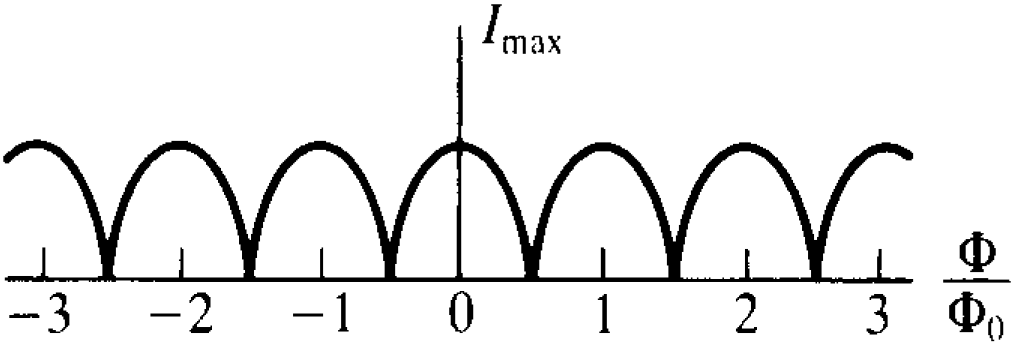
\includegraphics[width=0.6\textwidth]{immagini/SQUID_interference_pattern.png}
\end{figure}
\hspace{-0.6cm}Osserviamo una funzione oscillante, che rappresenta un vero e proprio pattern di interferenza, analogo a quello della doppia fenditura.\\
La differenza è che qui non stiamo osservando l'interferenza tra funzioni d'onda di singole particelle che attraversano due fenditure, ma l'interferenza tra le funzioni d'onda dei condensati superconduttivi che attraversano le due giunzioni Josephson. Le due giunzioni svolgono quindi il ruolo delle due fenditure.\\
Si tratta dunque di un pattern di interferenza di una funzione d'onda macroscopica, associata a un condensato formato da un numero macroscopico di elettroni descritti collettivamente da una singola funzione d'onda.\\
Questo fenomeno costituisce la base di magnetometri estremamente sensibili. Per capire il motivo, osserviamo con attenzione la regione del grafico in cui $\Phi/\Phi_0$ è prossimo a metà numero intero. Vediamo che piccolissime variazioni del campo magnetico applicato producono variazioni molto grandi della supercorrente. Di conseguenza, misurando la corrente superconduttiva possiamo ottenere informazioni estremamente precise su variazioni molto piccole del campo magnetico.\\
Facciamo attenzione al fatto che stiamo parlando di variazioni piccolissime della quantità $\Phi/\Phi_0$: questo significa che siamo in grado di rilevare variazioni di flusso magnetico confrontabili con una frazione del quanto di flusso.
\subsection{Fenomeni peculiari delle piccole giunzioni}
Finora abbiamo considerato l'effetto Josephson nel cosiddetto limite semiclassico, nel senso che la differenza di fase viene trattata come una variabile classica, pur avendo origine dalla meccanica quantistica. In questo contesto, quindi, la relazione di indeterminazione fase--numero che abbiamo già discusso per un superconduttore bulk non gioca alcun ruolo.\\
Quello che vedremo ora è che, se consideriamo giunzioni Josephson sufficientemente piccole, compare un comportamento in cui la natura di variabili coniugate di fase e numero diventa rilevante anche in un contesto quantistico. Ciò porterà a un effetto Josephson puramente quantistico.\\
Il punto è che oggi siamo in grado di realizzare elettrodi superconduttivi sufficientemente piccoli tali che la carica extra presente in queste piccole isole, anche a livello di singolo elettrone, diventi importante. In queste condizioni possiamo già intuire che la relazione di indeterminazione fase--numero, irrilevante nel caso di un superconduttore bulk, diventa invece significativa e conduce, come abbiamo detto, alla quantizzazione di fase e numero.\\
Vediamo innanzitutto quali siano le scale energetiche rilevanti e quali relazioni tra esse siano necessarie affinché emergano fenomeni quantistici. Consideriamo schematicamente un dispositivo del tipo seguente:
\begin{figure}[H]
    \centering
    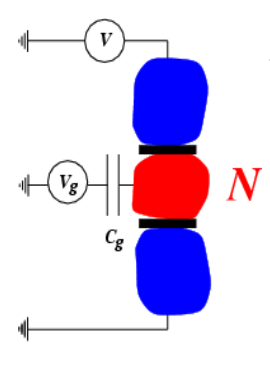
\includegraphics[width=0.27\textwidth]{immagini/single_electron_tunneling_geometry.png}
\end{figure}
\hspace{-0.6cm}Supponiamo di avere due elettrodi costituiti da metalli normali separati da uno strato isolante, per cui il dispositivo rappresentato è una giunzione NIN. Gli elettrodi sono generalmente collegati sia a un circuito di gate, che fissa il potenziale dell'isola centrale, sia a una tensione di trasporto.\\
In queste condizioni, poiché stiamo considerando elettrodi molto piccoli, tali elettrodi vengono spesso chiamati \emph{grains}. Questa è la tipica geometria di un dispositivo a tunneling di singolo elettrone. Abbiamo già discusso in passato che, anche nel caso di elettrodi normali, la presenza di due elettrodi affacciati implica un effetto capacitivo, per cui possiamo definire una capacità di giunzione, legata al costo elettrostatico associato alla presenza di cariche extra, ad esempio sull'isola centrale.\\
L'energia elettrostatica minima corrisponde naturalmente al caso in cui sia presente un elettrone aggiuntivo sull'isola. Tale configurazione comporta un costo energetico chiamato \emph{charging energy}:
\begin{equation*}
    E_C
    =
    \frac{e^2}{2C}
\end{equation*}
dove $C$ è la capacità della giunzione. Questa rappresenta una scala energetica fondamentale quando si considerano elettrodi di dimensioni ridotte.\\
Inoltre, per questo circuito possiamo definire anche una resistenza di tunneling, cioè una resistenza associata agli effetti dissipativi dovuti alla presenza dello strato isolante.\\
Per stimare quando gli effetti di carica diventano rilevanti, dobbiamo confrontare innanzitutto l'energia di carica con l'energia termica. La scala energetica delle fluttuazioni termiche è infatti $k_B T$. Per poter osservare effetti di carica dobbiamo quindi richiedere che si abbia
\begin{equation*}
    E_C > k_B T
\end{equation*}
Dobbiamo tenere presente che il nostro interesse è rivolto a elettrodi superconduttivi, quindi a temperature piuttosto basse. Ad esempio, a $T=1\;\rm K$, l'energia elettrostatica associata a un singolo elettrone risulta maggiore dell'energia termica purché la capacità sia minore di circa $10^{-15}\,\rm F$. Utilizzando l'espressione classica della capacità per una geometria piana, ciò corrisponde a un'area della giunzione inferiore a circa $10^{-8}\,\rm cm^2$.\\
Questo ci fornisce già un ordine di grandezza delle dimensioni necessarie affinché gli effetti di carica siano osservabili a temperature dell'ordine di pochi Kelvin, cioè proprio le temperature a cui si manifesta la superconduttività.\\
Oltre a ciò, stiamo considerando sistemi quantistici e sappiamo che, in generale, per sistemi quantomeccanici esiste una relazione di indeterminazione che collega l'incertezza in energia al tempo caratteristico del fenomeno. Se consideriamo l'incertezza associata all'energia di carica necessaria per osservare effetti quantistici, dobbiamo avere
\begin{equation*}
    \Delta E_C
    >
    \frac{\hbar}{\Delta t}
    \approx
    \frac{\hbar}{RC},
\end{equation*}
dove $\Delta t$ rappresenta la scala temporale tipica del circuito. In un sistema in cui avviene tunneling, tale tempo può essere stimato tramite il tempo caratteristico $RC$, con $C$ capacità della giunzione. Questo tempo rappresenta approssimativamente il tempo medio durante il quale un singolo elettrone rimane confinato sull'isola.\\
Se consideriamo un'incertezza energetica dell'ordine dell'energia di carica, dalla relazione di indeterminazione otteniamo allora una condizione sulla resistenza:
\begin{equation*}
    \Delta E
    \sim
    \frac{e^2}{2C}
    \implies
    R
    >
    \frac{2\hbar}{e^2}
    \equiv
    R_Q
    \sim
    6\;\rm k\Omega.
\end{equation*}
La resistenza deve quindi essere maggiore di una quantità chiamata \emph{quanto di resistenza}. Tale nome non significa che essa derivi direttamente da un effetto quantistico, ma che compare naturalmente applicando la relazione di indeterminazione energia--tempo all'energia di carica associata a un singolo elettrone. Questo è quindi il regime di condizioni che le giunzioni devono soddisfare affinché diventino osservabili effetti legati all'energia di carica di un singolo elettrone.
\subsection{Relazioni di indeterminazione fase--numero nelle giunzioni Josephson}
Quello che vogliamo capire ora è quando, in queste condizioni, diventano visibili anche gli effetti associati alla relazione di indeterminazione tra fase e numero. A questo scopo, riassumiamo innanzitutto ciò che sappiamo già per un superconduttore bulk.\\
Sappiamo che lo stato fondamentale di un superconduttore bulk ha la forma
\begin{equation*}
    \ket*{g_s}
    =
    \prod_{\vb{k}}
    \bigl(
        u_{\vb{k}}
        +
        \nu_{\vb{k}} Z_{\vb{k}}^{\dag}
    \bigr)
    \ket*{0}
\end{equation*}
Questa forma esplicita implica che la fase relativa tra componenti con differente numero di particelle è fissata. Possiamo vederlo nel modo seguente. Consideriamo lo stato
\begin{equation*}
    \ket*{\psi_{\phi}}
    =
    \prod_{\vb{k}}
    \bigl(
        u_{\vb{k}}
        +
        \nu_{\vb{k}} e^{i\phi} Z_{\vb{k}}^{\dag}
    \bigr)
    \ket*{0}
\end{equation*}
che differisce dal precedente per la presenza di un fattore di fase $e^{i\phi}$ associato alla creazione di ogni coppia di Cooper.\\
Abbiamo già visto che questo stato, che non possiede un numero fissato di particelle, può essere scritto come combinazione lineare di stati a numero fissato di particelle $\ket*{\psi_N}$:
\begin{equation*}
    \ket*{\psi_{\phi}}
    =
    \sum_N
    \lambda_N
    e^{i\phi N/2}
    \ket*{\psi_N}
\end{equation*}
Se associamo quindi una fase $\phi$ a ogni coppia di Cooper, decomponendo lo stato in una sovrapposizione di stati con diverso numero di coppie otteniamo, davanti a ciascuno stato $\ket*{\psi_N}$ con numero fissato di elettroni, un fattore di fase $e^{i\phi N/2}$.\\
Questa scrittura mostra immediatamente che, ogni volta che fissiamo una fase $\phi$, il numero di particelle diventa incerto, poiché per ciascun valore della fase abbiamo una sovrapposizione di stati con differente numero di particelle.\\
Abbiamo inoltre visto che, per estrarre da questa combinazione lineare la componente con un numero fissato di particelle, diciamo $N'$, dobbiamo rendere completamente incerta la fase. Questo significa considerare lo stato ottenuto moltiplicando $\ket*{\psi_{\phi}}$ per il fattore $e^{-i\phi N'/2}$ e integrando poi su tutti i valori della fase tra $0$ e $2\pi$:
\begin{equation*}
    \begin{split}
        \int_0^{2\pi}
        \dd{\phi}
        e^{-i\phi N'/2}
        \ket*{\psi_{\phi}}
        &=
        \int_0^{2\pi}
        \dd{\phi}
        \sum_N
        \lambda_N
        e^{i\phi N/2}
        e^{-i\phi N'/2}
        \ket*{\psi_N}
        \\[0.2cm]
        &=
        \sum_N
        \lambda_N
        2\pi
        \delta_{N,N'}
        \ket*{\psi_N}
        \\[0.2cm]
        &=
        2\pi
        \lambda_{N'}
        \ket*{\psi_{N'}}
    \end{split}
\end{equation*}
Questo è un modo per mostrare che, per estrarre dallo stato $\ket*{\psi_{\phi}}$ la componente con numero fissato di particelle $N'$, dobbiamo rendere completamente incerta la fase, cioè integrare su tutti i possibili valori di $\phi$.\\
Consideriamo ora in particolare la relazione
\begin{equation*}
    \int_0^{2\pi}
    \dd{\phi}
    e^{-i\phi N'/2}
    \ket*{\psi_{\phi}}
    =
    2\pi
    \lambda_{N'}
    \ket*{\psi_{N'}}
\end{equation*}
Questa espressione ricorda molto ciò che si fa in meccanica quantistica ordinaria quando, nella rappresentazione delle coordinate, integriamo su tutte le posizioni possibili un'onda piana con momento fissato $k$:
\begin{equation*}
    \int_{-\infty}^{\infty}
    \frac{\dd{x}}{2\pi}
    e^{-ikx}
    \ket*{x}
    =
    \ket*{k}
\end{equation*}
In quel caso, rendere completamente incerta la posizione permette di ottenere uno stato a momento fissato. Questo porta alla relazione di indeterminazione tra posizione e quantità di moto, oppure, equivalentemente, tra posizione e vettore d'onda:
\[
\Delta x \Delta k \sim \frac{1}{2}.
\]
In maniera del tutto analoga, la corrispondenza formale con la relazione appena ottenuta suggerisce una relazione di indeterminazione tra numero di particelle e fase:
\[
\Delta N \Delta\phi \sim 1.
\]
Questa è proprio la relazione di indeterminazione fase--numero che abbiamo già incontrato.\\
Nel caso di un superconduttore bulk, avere un numero non fissato di particelle non costituisce un problema, perché l'incertezza relativa sul numero di particelle, che scala come l'inverso della radice quadrata del numero medio di particelle, risulta estremamente piccola:
\begin{equation*}
    \frac{\delta N}{\bar{N}}
    \sim
    \frac{\sqrt{T_c/T_F}}{\sqrt{N}}
    \sim
    10^{-13}
\end{equation*}
Questo significa che, anche se lo stato fondamentale di un superconduttore bulk non possiede un numero esatto di particelle, ciò non ha conseguenze fisicamente rilevanti.\\
La situazione cambia quando consideriamo un piccolo pezzo di superconduttore. In questo caso, avere un differente numero di particelle significa avere una differente quantità di carica elettrica, e quindi una diversa energia elettrostatica. Di conseguenza, l'incertezza nel numero di particelle diventa fisicamente importante.\\
A questo punto possiamo spingerci oltre questa analogia tra fase e numero. Poiché la fase è una variabile periodica, se la interpretiamo come una coordinata, la variabile coniugata associata deve essere discreta, in modo del tutto analogo a quanto accade per il momento angolare.\\
Facciamo quindi un ulteriore passo introducendo una quantizzazione fenomenologica. Abbiamo infatti due variabili caratteristiche dello stato quantistico del sistema, e abbiamo trovato tra esse una relazione di indeterminazione. Decidiamo quindi di trattarle come variabili quantistiche e, come conseguenza della relazione di indeterminazione, introduciamo una relazione di commutazione canonica tra fase e numero:
\begin{equation*}
    [\hat{\phi},\hat{N}]
    =
    i
\end{equation*}
Se vogliamo scrivere questa relazione in forma più simile alla relazione di commutazione posizione--momento, dobbiamo moltiplicare per $\hbar$. Inoltre, per rendere esplicito il fatto che le cariche rilevanti sono le coppie di Cooper, definiamo l'operatore $\hat{Q}$ come numero di coppie di Cooper:
\begin{equation*}
    \qty[
        \frac{\hbar}{2}\hat{\phi},
        2\hat{Q}
    ]
    =
    i\hbar.
\end{equation*}
Una volta quantizzate fase e numero, possiamo dire che lo stato BCS, essendo caratterizzato da una fase ben definita, è un autostato dell'operatore fase.\\
Così come esistono autofunzioni della fase, esistono anche autofunzioni del numero, che diventano gli autostati naturali del sistema quando la configurazione superconduttiva considerata è dominata dagli effetti di carica. In altre parole, quando l'energia elettrostatica è la scala energetica dominante, gli autostati del sistema sono gli autostati dell'operatore carica.\\
Vogliamo ora avvicinarci gradualmente al caso di una giunzione Josephson. Consideriamo quindi due superconduttori bulk e immaginiamo di avvicinarli tra loro. Il sistema formato da questi due superconduttori tenderà a raggiungere una configurazione di minima energia.\mn{Nelle slide compare la frase: ``If two SC are brought close enough, the system tends to a lower energy configuration by tunneling (similar to a molecular bond).''}\\
Questa configurazione di minima energia deve tenere conto dei processi di tunneling elettronico da un lato all'altro della giunzione. Per descrivere lo stato complessivo dei due superconduttori dobbiamo quindi considerare la possibilità che alcuni elettroni siano passati da un lato all'altro, anche se non sappiamo quanti.\\
Possiamo allora scrivere lo stato generale dei due superconduttori vicini come una sovrapposizione degli stati $\ket*{\psi^L}$ e $\ket*{\psi^R}$ dei due elettrodi. In linea di principio, tali stati possono contenere differenti numeri di cariche trasferite da una parte all'altra.\\
Supponiamo che inizialmente entrambi i superconduttori contengano $N$ elettroni. Possiamo allora avere stati in cui un certo numero di elettroni, diciamo $q$, è tunnelato da un lato all'altro. Poiché non sappiamo quale sia il valore effettivo di $q$, dobbiamo considerare una sovrapposizione di tutti questi stati:
\begin{equation*}
    \ket*{\psi}
    =\sum_q a_q \ket*{\psi^L_{N+q}} \hspace{-0.17cm} \ket*{\psi^R_{N-q}}
\end{equation*}
Sappiamo già che questi numeri di particelle non sono fissati esattamente. Questo implica una certa incertezza sulla fase, anche se non così estrema come nel caso di numero completamente fissato.\\
Una volta scritto questo stato, dobbiamo tenere presente che, poiché i numeri di particelle non sono fissati, possono esistere fluttuazioni. Tali fluttuazioni si manifestano sui due lati della giunzione, e quindi avremo un'incertezza su $q$. Il fatto stesso che nello stato compaiano tutti i valori di $q$ equivale a dire che esiste un'incertezza sulla carica trasferita.\\
Ma una differenza di carica tra i due lati implica anche una differenza di energia elettrostatica. In altre parole, uno stato di questo tipo corrisponde a una configurazione in cui compare una carica sui due lati della giunzione, con il conseguente costo energetico associato.\\
Se immaginiamo matematicamente il limite in cui l'energia di carica $E_C$ tende a zero, è chiaro che, in assenza di costo elettrostatico, ciascun elettrodo superconduttivo resterà nello stato di minima energia, cioè in uno stato a fase fissata. In questo caso le due fasi sono semplicemente variabili classiche, esattamente come nella descrizione semiclassica sviluppata finora.\\
La presenza di un'energia di carica, cioè il fatto che esista un costo energetico associato a cariche extra sui due lati della giunzione, implica invece che il sistema cerchi di minimizzare tali cariche aggiuntive. Questo conduce a una relazione di indeterminazione e quindi a un comportamento quantistico della differenza di fase $\varphi$ tra i due elettrodi.\\
Queste fluttuazioni quantistiche della fase implicano che, quando consideriamo due superconduttori affacciati l'uno di fronte all'altro includendo il tunneling di carica e l'energia elettrostatica, la differenza di fase e lo sbilanciamento di carica tra i due lati soddisfano anch'essi una relazione di indeterminazione.\\
Possiamo allora imporre fenomenologicamente anche in questo caso una relazione di commutazione tra la differenza di fase e lo sbilanciamento di carica:
\begin{equation*}
    \qty[
        \hat{\varphi},
        \hat{n}
    ]
    =
    i,
\end{equation*}
dove
\begin{equation*}
    \hat{\varphi}=\hat{\phi}_2-\hat{\phi}_1
    \qq{e}
    \hat{n}=\frac{\hat{n}_2-\hat{n}_1}{2}
\end{equation*}
Quello che stiamo facendo, quindi, è passare gradualmente dalla relazione di indeterminazione fase--numero per un singolo superconduttore alla relazione di indeterminazione tra differenza di fase e sbilanciamento di carica in una giunzione Josephson.\\
Possiamo infine riscrivere questa relazione in forma analoga a quella già ottenuta:
\begin{equation*}
    \qty[ \frac{\hbar}{2}\hat{\varphi},2\hat{Q}]
    =i\hbar
\end{equation*}
\section{Descrizione circuitale}
\subsection{Descrizione circuitale (classica) riformulata in termini della fase}
A questo punto vogliamo considerare circuiti che includono una giunzione Josephson sufficientemente piccola affinché gli effetti di carica diventino rilevanti.\\
Innanzitutto scriveremo le equazioni circuitali. Se abbiamo una giunzione Josephson inserita in un circuito, dobbiamo infatti scrivere le equazioni del circuito, cioè le relazioni elettrodinamiche, tenendo conto della relazione non lineare caratteristica dell'elemento Josephson. Successivamente vedremo che cosa accade quando quantizziamo carica e differenza di fase, in particolare otterremo quindi un'equazione circuitale trattata quantisticamente.\\
Partiamo dalla descrizione circuitale classica, riformulandola però in termini della fase. In questo contesto dobbiamo considerare le due relazioni di Josephson come relazioni costitutive dell'elemento circuitale rappresentato dalla giunzione Josephson, che convenzionalmente viene indicata con una croce.\\
Le due relazioni di Josephson collegano la corrente attraverso la giunzione e la differenza di potenziale ai capi della giunzione con la differenza di fase:
\begin{equation*}
    I=I_0 \sin{\phi_{LR}}
    \qq{,}
    V=\frac{\hbar}{2e}\dot{\phi}_{LR}
\end{equation*}
Inseriamo ora questa giunzione Josephson all'interno di un circuito. Per descrivere il circuito dobbiamo scegliere una convenzione per orientare corrente e differenza di potenziale. Utilizziamo la stessa convenzione dell'elettromagnetismo classico, cioè assumiamo che la corrente sia positiva da sinistra verso destra quando il potenziale a sinistra è maggiore di quello a destra:
\begin{equation*}
    V=V_L-V_R>0
    \implies
    I^{\text{L}\to\text{R}}>0
\end{equation*}
In questo modo tutto resta coerente con la legge di Ohm e con la convenzione usuale per i circuiti resistivi.\\
Questo vale per una singola giunzione. In generale, però, la giunzione farà parte di un circuito chiuso. Tale circuito potrà contenere capacità, induttanze o altri elementi circuitali.\\
Abbiamo inoltre visto che, quando una giunzione interrompe un anello superconduttivo, esiste una relazione tra la differenza di fase ai capi della giunzione e il flusso magnetico concatenato con l'anello:
\begin{equation*}
    \Phi=\frac{\hbar}{2e}\varphi
\end{equation*}
Poiché l'effetto Josephson implica che una differenza di fase variabile nel tempo produca una tensione, mettendo insieme questa relazione con quella che lega la fase al flusso otteniamo la legge di Faraday--Neumann--Lenz:
\begin{equation*}
    V = \frac{\hbar}{2e}\dot{\phi}_{LR} \equiv \dot{\Phi}
\end{equation*}
Un ulteriore punto importante è che, in presenza di un campo magnetico esterno, dobbiamo utilizzare quantità gauge-invarianti, in particolare la differenza di fase gauge-invariante.\\
Abbiamo visto che la differenza di fase gauge-invariante tra i due elettrodi sinistro e destro è
\begin{equation*}
    \gamma_L-\gamma_R
    =
    \phi_L-\phi_R
    -
    \frac{2\pi}{\Phi_0}
    \int_L^R
    \vb{A}\vdot\dd{\vb{s}},
\end{equation*}
dove il secondo termine rappresenta il contributo del potenziale vettore lungo un percorso interno alla giunzione.\\
In questo caso il flusso magnetico risulta collegato alla differenza di fase gauge-invariante, e anche la corrente Josephson dipende da essa:
\begin{equation*}
    \Phi
    =
    \frac{\hbar\gamma_{LR}}{2e}
    \qq{,}
    I_J
    =
    I_0 \sin{\gamma_{LR}}
\end{equation*}
La tensione resta invece legata alla derivata temporale della fase, mentre la derivata temporale del flusso magnetico è collegata al rapporto tra carica e capacità:
\begin{equation*}
    V_{LR}
    =
    \frac{\hbar\dot{\phi}_{LR}}{2e}
    \qq{,}
    \dot{\Phi}
    =
    \frac{Q}{C}
    =
    \int
    \vb{E}\vdot\dd{\vb{s}}
\end{equation*}
Queste sono quindi le relazioni elettrodinamiche che collegano i diversi elementi circuitali.\\
Questo tipo di descrizione circuitale conduce naturalmente all'espressione dell'energia immagazzinata in un elemento Josephson. Vedremo infatti che essa può essere scritta in termini di una scala energetica chiamata energia Josephson, proporzionale alla corrente critica della giunzione, moltiplicata per un termine del tipo $1-\cos{\varphi}$, mentre la corrente dipende come $\sin{\varphi}$.\\
Per vedere come emerga questa struttura, consideriamo che l'energia associata alla giunzione Josephson può essere interpretata come il lavoro elettrico compiuto dalla corrente nel caricare la giunzione:
\begin{equation*}
    E
    =
    \int_0^{t'}
    \dd{t'}
    V(t')
    I_J(t').
\end{equation*}
Usando le relazioni di Josephson possiamo riscrivere l'integrale come
\begin{equation*}
    E
    =
    \int_0^{t'}
    \dd{t'}
    \frac{\hbar}{2e}
    \dot{\phi}_{LR}(t')
    I_0
    \sin{\phi_{LR}(t')}
\end{equation*}
Effettuando il cambio di variabile otteniamo
\begin{equation*}
    E
    =
    \frac{\hbar I_0}{2e}
    \int_{\varphi(0)}^{\varphi(t')}
    \dd{\varphi}
    \sin{\varphi}
    =
    E_J
    \bigl[
        1-\cos{\varphi(t')}
    \bigr],
\end{equation*}
dove abbiamo assunto $\varphi(0)=0$ e definito l'energia Josephson come
\begin{equation*}
    E_J=\frac{\hbar I_0}{2e}
\end{equation*}
Questa quantità rappresenta quindi semplicemente il lavoro elettrico necessario a caricare la giunzione.\\
Vediamo quindi che stiamo gradualmente identificando tutti gli elementi circuitali e le corrispondenti energie necessarie per descrivere circuiti contenenti giunzioni Josephson.\\
In particolare possiamo usare le usuali rappresentazioni circuitali, reinterpretandole in termini della differenza di fase e del flusso magnetico:
\begin{itemize}[leftmargin=0.5cm]
    \item Resistenza: $V=RI_R \quad\Rightarrow\quad I_R=\frac{\dot{\Phi}}{R}$
    \item Capacità:
    $
    Q=CV
    \quad\Rightarrow\quad
    I_C=\dot{Q}=C\ddot{\Phi}
    $
    \item Induttanza:
    $
    V=L\dot{I}_L
    \quad\Rightarrow\quad
    I_L
    =
    \frac{1}{L}
    \int_0^t
    \dd{t}\,V
    =
    \frac{\Phi}{L}.
    $
\end{itemize}
A questo punto possiamo fare un'ulteriore osservazione.
\begin{figure}[H]
    \centering
    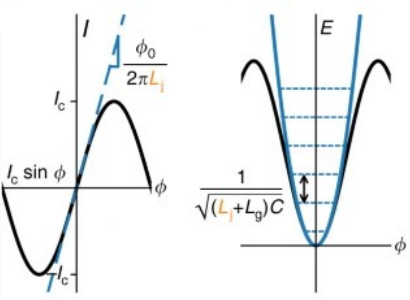
\includegraphics[width=0.5\textwidth]{immagini/josephson_energy_and_current.png}
\end{figure}
\hspace{-0.6cm}Abbiamo visto che l'energia Josephson è una funzione periodica che si annulla per $\varphi=0$. Se consideriamo il primo minimo della funzione, il potenziale appare approssimativamente parabolico nelle vicinanze del minimo stesso.\\
La corrente Josephson è anch'essa una funzione periodica che si annulla per $\varphi=0$, e per piccoli valori della fase è praticamente lineare:
\begin{equation*}
    I=I_J \sin{\varphi} \approx I_J \varphi
\end{equation*}
Analogamente, per piccoli valori di $\varphi$, possiamo approssimare l'energia come
\begin{equation*}
    E
    =E_J \bigl[ 1 - \cos{\varphi} \bigr]
    \approx E_J \qty[ 1 - \qty(1 - \frac{\varphi^2}{2}) ]
    =E_J\frac{\varphi^2}{2}
\end{equation*}
Quindi, per piccole oscillazioni della fase, il potenziale è approssimativamente armonico e la corrente dipende linearmente dalla fase.\\
In queste condizioni possiamo definire una induttanza equivalente della giunzione. Infatti:
\begin{equation*}
    I_J
    \approx
    I_0\varphi
    =
    I_0
    \frac{2e}{\hbar}
    \Phi.
\end{equation*}
Da questa relazione definiamo l'induttanza Josephson lineare:
\begin{equation*}
    L_{J,0}
    =
    \frac{\hbar}{2eI_0}
    =
    \frac{\Phi_0}{2\pi I_0}.
\end{equation*}
In generale, poiché la relazione corrente--fase non è lineare, anche l'induttanza sarà non lineare.\\
Allo stesso modo, dall'espressione dell'energia della giunzione possiamo definire una frequenza di oscillazione vicino al minimo del potenziale, detta frequenza di plasma Josephson. Essa dipende sia dall'induttanza sia dalla capacità della giunzione:
\begin{equation*}
    \omega_{p,0}
    =
    \frac{1}{\sqrt{L_{J,0}C}}
    =
    \sqrt{
        \frac{2\pi I_0}{C\Phi_0}
    }
\end{equation*}
La ragione per cui introduciamo tutte queste quantità è che esse permettono di identificare le scale energetiche caratteristiche della giunzione quando questa fa parte di un circuito.\\
Le due energie fondamentali sono:
\begin{itemize}[leftmargin=0.5cm]
    \item l'energia di carica, che ora scriviamo in termini della carica di una coppia di Cooper, e che rappresenta il costo elettrostatico associato al tunneling di due elettroni attraverso la giunzione;
    \item l'energia Josephson, cioè la scala energetica associata al termine Josephson dell'hamiltoniana.
\end{itemize}
Queste due energie si combinano nella frequenza di plasma:
\begin{equation*}
    \omega_{p,0}
    =
    \sqrt{2E_JE_C},
    \qquad
    E_C
    =
    \frac{(2e)^2}{2C},
    \qquad
    E_J
    =
    \frac{\hbar I_0}{2e}.
\end{equation*}
Vediamo quindi che:
\begin{itemize}[leftmargin=0.5cm]
    \item l'energia di carica dipende inversamente dalla capacità, quindi per giunzioni grandi $E_C$ è piccola;
    \item l'energia Josephson dipende invece dalla corrente critica e quindi dalle proprietà microscopiche della giunzione e dall'ampiezza di tunneling.
\end{itemize}
A seconda delle dimensioni e del materiale della giunzione possiamo quindi trovarci in due regimi distinti: $E_C \gg E_J$ oppure $E_J \gg E_C$.\\
Che cosa comportano questi due limiti per carica e fase? Per capirlo possiamo usare un'analogia con la meccanica quantistica di una particella soggetta a energia cinetica ed energia potenziale.\\
Se il termine dominante nell'hamiltoniana è il potenziale, gli autostati del sistema saranno autostati della coordinata. Se invece domina l'energia cinetica, gli autostati saranno onde piane, cioè autostati dell'impulso.\\
Le energie $E_C$ ed $E_J$ giocano un ruolo del tutto analogo:
\begin{itemize}[leftmargin=0.5cm]
    \item se domina l'energia di carica, gli autostati del sistema saranno stati a carica definita. La carica sarà quindi ben definita, mentre la fase sarà fortemente incerta;
    \item se domina l'energia Josephson, gli autostati saranno invece stati a fase ben definita, analogamente allo stato fondamentale BCS. In questo caso sarà la carica a diventare incerta.
\end{itemize}
Dobbiamo quindi interpretare queste due energie come l'analogo, rispettivamente, dell'energia cinetica e dell'energia potenziale, con la fase che gioca il ruolo della coordinata.\\
Abbiamo sviluppato tutte queste considerazioni perché ci serviranno per analizzare circuiti contenenti giunzioni Josephson in differenti regimi fisici.\\
Questi circuiti costituiscono infatti i mattoni fondamentali di molte applicazioni basate sulla superconduttività: dalla realizzazione di magnetometri estremamente sensibili fino, nel limite di dimensioni sempre più piccole, ai circuiti superconduttivi utilizzati come elementi base per il calcolo quantistico.
\subsection{Il modello RCSJ}
Il modello più semplice che consideriamo è quello di una giunzione Josephson reale. Una giunzione Josephson possiede infatti una capacità intrinseca, per cui dobbiamo includere nel modello una capacità in parallelo. Inoltre, abbiamo detto che anche in una giunzione Josephson ideale sono presenti impurità ed effetti dissipativi, dovuti ad esempio alla temperatura finita e alla presenza di quasiparticelle. Di conseguenza, dobbiamo considerare anche una componente resistiva in parallelo alla giunzione Josephson.\\
In modo qualitativo, maggiore è la resistenza, maggiore sarà la frazione di corrente che attraversa la giunzione Josephson, e viceversa. Per questo motivo possiamo modellizzare una giunzione Josephson reale come una giunzione ideale posta in parallelo con un condensatore e una resistenza:
\begin{figure}[H]
    \centering
    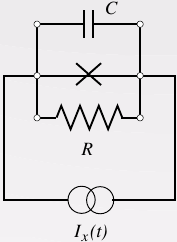
\includegraphics[width=0.3\textwidth]{immagini/RCSJ_model.png}
\end{figure}
\hspace{-0.6cm}Questo rappresenta quindi il blocco fondamentale costituito dalla giunzione Josephson ideale, dalla sua capacità e dagli effetti dissipativi.\\
In generale, la giunzione non è isolata, ma fa parte di un circuito. In particolare consideriamo il caso in cui il circuito sia polarizzato in corrente, cioè contenga un generatore di corrente.\\
Questo tipo di circuito prende il nome di modello RCSJ (\textit{Resistively and Capacitively Shunted Josephson Junction}).\\
L'equazione circuitale si scrive molto semplicemente osservando che la corrente di bias $I_x$, arrivando al nodo, si divide nei diversi rami:
\begin{equation}
    I_x=I_C + I_R + I_J
\end{equation}
Esprimiamo ora i vari contributi in termini delle grandezze circuitali e, in particolare, del flusso magnetico nel circuito:
\begin{equation}
    I_x
    =
    C \ddot{\Phi}
    +
    \frac{\dot{\Phi}}{R}
    +
    I_0
    \sin{
        \qty(
            \frac{2\pi\Phi}{\Phi_0}
        )
    }
    \label{eq:circuit_equation_RCSJ}
\end{equation}
Abbiamo ottenuto semplicemente un'equazione differenziale del secondo ordine che descrive il circuito contenente questi tre elementi.\\
Dimentichiamo ora momentaneamente il circuito e consideriamo invece una particella di coordinata $x$. L'equazione del moto di una particella soggetta a un potenziale e a dissipazione è
\begin{equation*}
    m\ddot{x}
    +
    \eta\dot{x}
    +
    U'(x)
    =
    0.
\end{equation*}
Notiamo che l'equazione circuitale \eqrefcustom{eq:circuit_equation_RCSJ} ha esattamente la stessa struttura: al posto della coordinata compare il flusso magnetico $\Phi$, il termine capacitivo gioca il ruolo dell'energia cinetica, il termine Josephson quello dell'energia potenziale, mentre la resistenza introduce dissipazione.\\
In altre parole, l'equazione del circuito è equivalente a quella di una particella di massa efficace proporzionale alla capacità, che si muove in un potenziale tale che
\begin{equation*}
    U'(\Phi)=I_0 \sin{ \qty( \frac{2\pi\Phi}{\Phi_0} )} - I_x
\end{equation*}
Integrando rispetto a $\Phi$, otteniamo il potenziale:
\begin{equation*}
    U(\Phi)=-E_J \cos{ \qty( \frac{2\pi\Phi}{\Phi_0} ) } - I_x\Phi
\end{equation*}
Vediamo quindi che il potenziale dipende dalla corrente di bias, che è un parametro controllabile esternamente, mentre l'energia Josephson e la capacità sono fissate una volta costruita la giunzione.\\
Vediamo ora come varia $U$ in funzione di $\Phi$:
\begin{figure}[H]
    \centering
    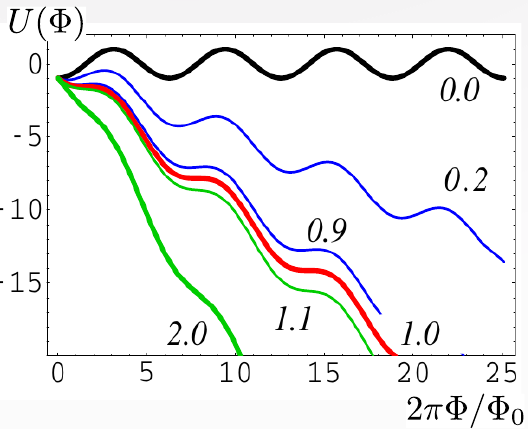
\includegraphics[width=0.55\textwidth]{immagini/potential_RCSJ.png}
\end{figure}
\hspace{-0.6cm}Le diverse curve corrispondono a differenti valori della corrente normalizzata $i_x=\frac{I_x}{I_0}$, cioè della corrente di bias in unità della corrente critica.\\
Consideriamo innanzitutto il caso $i_x=0$, cioè assenza di corrente di bias. In questo caso il potenziale coincide semplicemente con il potenziale sinusoidale Josephson.\\
Se invece la corrente di bias è diversa da zero, compare un termine lineare con segno negativo che inclina il potenziale. Il potenziale quindi non sarà più perfettamente periodico con la stessa ampiezza, ma risulterà progressivamente inclinato. Per piccoli valori della corrente di bias la forma resta simile a quella sinusoidale, ma compare una pendenza globale. All'aumentare della corrente di bias aumenta anche l'inclinazione del potenziale.\\
Finché $i_x\leq1$ il potenziale continua comunque a possedere minimi locali.\\
Questo si vede facilmente derivando il potenziale:
\begin{equation*}
    U'(\Phi)=0
    \quad\Longrightarrow\quad
    I_0 \sin{\qty(\frac{2\pi\Phi}{\Phi_0})}
    =I_x
\end{equation*}
cioè
\begin{equation*}
    \sin{\qty(\frac{2\pi\Phi}{\Phi_0})}
    =\frac{I_x}{I_0}
    =i_x
\end{equation*}
Questa equazione può avere soluzione soltanto per $i_x\leq1$. Ciò significa che il potenziale possiede minimi stabili soltanto quando la corrente di bias è minore o uguale alla corrente critica. Quando invece $i_x>1$, non esistono più minimi né massimi locali. Infatti, osservando ad esempio la curva corrispondente a $i_x=2$, vediamo che il potenziale risulta completamente inclinato.\\
Quello che vogliamo fare ora è capire qualitativamente come si comporta il circuito nei diversi regimi. Quando la corrente di bias è minore della corrente critica, il comportamento del circuito può essere compreso sfruttando l'analogia con una particella che si muove in un potenziale di questo tipo. Che cosa succede infatti a una particella soggetta a un potenziale come questo? Se la particella si trova in un minimo del potenziale, esistono due possibilità: o possiede energia sufficiente per superare la barriera, oppure non la possiede e quindi resta confinata nel minimo.\\
Naturalmente questa è ancora una descrizione classica. Nel nostro caso, una particella intrappolata in un minimo significa che il flusso magnetico resta costante, poiché la coordinata della particella resta fissa nel minimo del potenziale. Ma un flusso costante implica assenza di differenza di potenziale. Di conseguenza, il circuito presenta una corrente continua dovuta all'effetto Josephson, senza caduta di tensione: abbiamo cioè il classico effetto Josephson DC, ovvero una supercorrente finita in assenza di tensione.
\subsection{Tunneling quantistico macroscopico}
Prima di entrare nella derivazione dettagliata del comportamento del circuito nei diversi regimi (poiché abbiamo differenti scale energetiche e quindi differenti regimi dinamici), vediamo un'importante applicazione di questo tipo di circuito, introdotta originariamente per mettere in evidenza il cosiddetto \emph{tunneling quantistico macroscopico}.\\
Questo nome può sembrare quasi contraddittorio, perché normalmente associamo il tunneling quantistico a particelle microscopiche ed elementari, mentre gli oggetti macroscopici non mostrano in genere proprietà quantistiche osservabili. In questo caso, però, ciò che effettua il tunneling è la funzione d'onda collettiva di un enorme numero di elettroni, cioè il condensato superconduttivo stesso. Vedremo quindi come un circuito di questo tipo possa fornire evidenza sperimentale di tale fenomeno.\\
Consideriamo una versione semplificata del modello in cui trascuriamo gli effetti resistivi, che, come abbiamo detto, derivano da quasiparticelle, impurità, eccetera. Rimane quindi soltanto il comportamento puramente superconduttivo:
\begin{figure}[H]
    \centering
    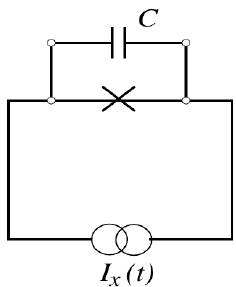
\includegraphics[width=0.35\textwidth]{immagini/CSJ_model.png}
\end{figure}
\hspace{-0.6cm}In questo caso otteniamo quella che viene chiamata \emph{capacitively shunted junction}. L'equazione circuitale si semplifica perché dobbiamo considerare soltanto la corrente attraverso la giunzione Josephson, la corrente di bias e quella che attraversa la capacità:
\begin{equation*}
    C \dv{V}{t}
    +
    I_c \sin{\varphi}
    =
    I_x(t)
\end{equation*}
Usando la seconda relazione di Josephson possiamo riscrivere il termine contenente la derivata della tensione come derivata seconda della fase:
\begin{equation*}
    C
    \frac{\hbar}{2e}
    \dv[2]{\varphi}{t}
    +
    I_c \sin{\varphi}
    =
    I_x(t)
\end{equation*}
Notiamo che, in questo caso, invece di scrivere l'equazione in funzione del flusso magnetico, la esprimiamo direttamente in termini della fase.\\
Moltiplicando entrambi i membri per $\frac{\hbar}{2e}$, otteniamo
\begin{equation*}
    C \qty( \frac{\hbar}{2e} )^2 \dv[2]{\varphi}{t} + \frac{\hbar}{2e} I_c \sin{\varphi} = \frac{\hbar}{2e} I_x(t)
\end{equation*}
Usando nuovamente l'analogia meccanica, questa equazione rappresenta il moto di una particella di coordinata $\varphi$ e massa efficace
\begin{equation*}
    m_{\rm eff}
    =
    C
    \qty(
        \frac{\hbar}{2e}
    )^2,
\end{equation*}
in un potenziale dato da
\begin{equation*}
    U(\varphi)
    = - \frac{\hbar}{2e} I_c \cos{\varphi} - \frac{\hbar}{2e} I_x \varphi
    = - E_J \cos{\varphi} - \frac{\hbar}{2e} I_x \varphi
\end{equation*}
Come nel caso precedente, il sistema è quindi equivalente a una particella che si muove in un potenziale che prende il nome di \emph{washboard potential}.\\
Facciamo ora un passo ulteriore: quantizziamo l'energia del sistema.\\
Abbiamo infatti una particella che si muove in questo potenziale; la coordinata è la fase $\varphi$, mentre la variabile coniugata è la carica. Poiché fase e carica soddisfano una relazione di indeterminazione, possiamo procedere alla quantizzazione del sistema e scrivere l'hamiltoniana quantistica associata.\\
Ricordiamo innanzitutto l'hamiltoniana classica di una particella:
\begin{equation*}
    H
    =
    \frac{p^2}{2m}
    +
    U(x),
\end{equation*}
che, una volta quantizzata, diventa
\begin{equation*}
    \hat{H}
    =
    \frac{\hat{p}^2}{2m}
    +
    U(\hat{x}).
\end{equation*}
Nel nostro caso il potenziale è $U(\varphi)$, che diventa quindi $U(\hat{\varphi})$, dove $\hat{\varphi}$ è l'operatore associato alla differenza di fase. Il termine cinetico è invece legato all'operatore carica, che è la variabile coniugata alla fase e gioca il ruolo dell'impulso.\\
Possiamo quindi scrivere l'hamiltoniana come
\begin{equation*}
    \hat{H}
    =
    \frac{\hat{Q}^2}{2C}
    +
    U(\hat{\varphi}).
\end{equation*}
Vediamo quindi che, attraverso questa quantizzazione fenomenologica, stiamo costruendo un'hamiltoniana che descrive un circuito elettrico contenente una giunzione Josephson. Questo è l'elemento concettualmente nuovo: quantizzare l'hamiltoniana di un circuito elettrico che include una giunzione Josephson.\\
Scriviamo ora esplicitamente i vari termini in funzione delle scale energetiche introdotte in precedenza. L'energia elettrostatica può essere espressa tramite l'energia di carica e l'operatore numero che conta le coppie di Cooper extra, mentre il termine potenziale è espresso in funzione dell'energia Josephson:
\begin{equation*}
    \hat{H}
    =
    E_C \hat{n}^2
    -
    E_J \cos{\hat{\varphi}}
    -
    \frac{\hbar}{2e}
    I_x
    \hat{\varphi}
\end{equation*}
A questo punto abbiamo tutti gli ingredienti necessari per comprendere qualitativamente ciò che accade. Consideriamo nuovamente il \emph{washboard potential}:
\begin{figure}[H]
    \centering
    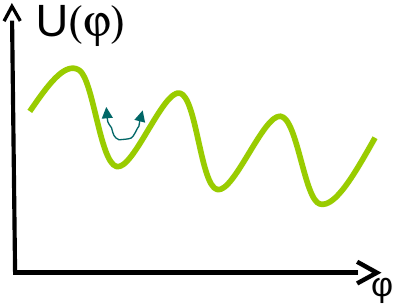
\includegraphics[width=0.4\textwidth]{immagini/washboard_potential.png}
\end{figure}
\hspace{-0.6cm}Se trattiamo il sistema come una particella quantistica di coordinata $\varphi$ in questo potenziale, sappiamo dalla meccanica quantistica che la particella non soltanto oscilla attorno a un minimo o supera classicamente la barriera se possiede energia sufficiente, ma può anche attraversare la barriera tramite tunneling quantistico.\\
Se quindi la particella non viene trattata classicamente, può effettuare tunneling tra minimi differenti del potenziale. Questo è consentito proprio perché stiamo trattando il circuito come un sistema quantistico.\\
A questo punto però dobbiamo chiederci: quale quantità fisica sta realmente effettuando il tunneling?\\
Ciò che attraversa la regione classicamente proibita è un numero macroscopico di particelle, cioè il condensato superconduttivo. In altre parole, si tratta del tunneling quantistico di un sistema macroscopico di elettroni. È proprio per questo motivo che il fenomeno prende il nome di \emph{tunneling quantistico macroscopico}.\\
Questo rappresenta il processo fisico profondo alla base dell'effetto Josephson.\\
Come possiamo osservare sperimentalmente tale fenomeno?\\
Se la particella si trova in un minimo del potenziale, il sistema si trova in uno stato a tensione nulla. Se però la particella effettua tunneling attraverso la barriera, una volta uscita dal minimo acquisisce tipicamente energia sufficiente per iniziare a ``scendere'' lungo il potenziale.\\
In termini dinamici, questo significa che la particella acquisisce una velocità non nulla, cioè una derivata temporale non nulla della fase:
\begin{equation*}
    \dot{\varphi}\neq0
\end{equation*}
Ma, per la relazione di Josephson, una variazione temporale della fase implica immediatamente la comparsa di una tensione ai capi della giunzione:
\begin{equation*}
    V
    =
    \frac{\hbar}{2e}
    \dot{\varphi}
\end{equation*}
Quindi, se il tunneling avviene, il valor medio della variabile quantistica $\hat{\varphi}$ cambia nel tempo e compare istantaneamente una tensione misurabile attraverso la giunzione.\\
Questo è precisamente il modo in cui viene rivelato sperimentalmente il tunneling quantistico macroscopico del condensato superconduttivo in un circuito di questo tipo.
\subsection{Osservabilità degli effetti quantistici nelle piccole giunzioni Josephson}
Commentiamo ora l'osservabilità di questi effetti quantistici.\\
Le energie che entrano in gioco sono quelle già discusse più volte: l'energia di carica, l'energia Josephson e la combinazione di queste due quantità che determina la frequenza di plasma.\\
Il comportamento della giunzione sarà essenzialmente classico, cioè caratterizzato semplicemente dal passaggio di corrente senza particolari effetti quantistici, quando gli effetti di carica sono trascurabili, cioè nel caso in cui $E_C \ll E_J$. In questo regime sappiamo che la carica è completamente indeterminata mentre la fase è ben definita, e si ottiene quindi il comportamento Josephson standard. Inoltre, la frequenza di plasma risulta molto più piccola dell'energia Josephson.\\
Gli effetti quantistici diventano invece rilevanti quando questa condizione non è più soddisfatta, cioè nel caso di giunzioni sufficientemente piccole, caratterizzate da capacità molto ridotte. Inoltre è necessario che la temperatura sia sufficientemente bassa, così da evitare la presenza di quasiparticelle eccitate che darebbero luogo a correnti dissipative.\\
Quello che serve quindi è avere un'energia di carica sufficientemente grande e, contemporaneamente, energie caratteristiche maggiori dell'energia termica.\\
Nella seguente tabella sono riportati gli ordini di grandezza tipici dell'area della giunzione, dell'energia Josephson, dell'energia di carica, della resistenza normale e della capacità per giunzioni realizzate in alluminio o niobio con barriera isolante realizzata con il relativo ossido.
\begin{table}[H]
    \centering
    \footnotesize
    \renewcommand{\arraystretch}{1.3}
    \begin{tabular}{|c|c|c|c|c|c|}
        \hline
        Giunzione & $A$ ($\mu$m$^2$) & $E_J$ ($\mu$eV) & $E_C$ ($\mu$eV) & $R_n$ ($\Omega$) & $C$ (pF) \\
        \hline
        Nb/NbO$_x$/PbIn & $10 \times 10$ & $2 \cdot 10^{4}$ & $5 \cdot 10^{-2}$ & $1.0$ & $\sim 10$ \\
        \hline
        Al/AlO$_x$/Al & $0.1 \times 0.1$ & $80.0$ & $470$ & $1000$ & $\sim 10^{-3}$ \\
        \hline
    \end{tabular}
    \caption*{
    Valori tipici dei parametri di giunzioni Josephson mesoscopiche in Nb ($J_c \approx 10\,\mathrm{A/cm^2}$) e di giunzioni ultrasmall in Al. In entrambi i casi la capacità specifica vale circa $c \approx 60\,\mathrm{fF/\mu m^2}$.}
\end{table}
\normalsize
\hspace{-0.6cm}La differenza principale tra questi due tipi di giunzioni è essenzialmente la loro dimensione. Le giunzioni in niobio sono tipicamente molto più grandi, con aree circa due ordini di grandezza maggiori rispetto alle giunzioni in alluminio.\\
Questo implica che:
\begin{itemize}[leftmargin=0.5cm]
    \item nelle grandi giunzioni l'energia di carica è molto piccola;
    \item nelle piccole giunzioni l'energia di carica diventa invece significativa;
    \item la capacità segue naturalmente l'andamento opposto.
\end{itemize}
Vi sono inoltre differenze anche nell'energia Josephson. Nel caso di giunzioni grandi (dove ``grande'' si riferisce all'area laterale, poiché lo spessore della barriera resta sempre dell'ordine di pochi nanometri affinché il tunneling sia possibile), la superficie dei superconduttori separati dalla barriera isolante è maggiore. Ciò implica un'ampiezza di tunneling più elevata e quindi un'energia Josephson maggiore.\\
In maniera qualitativa possiamo dire che, quanto più grande è la giunzione, tanto maggiore è la probabilità che un numero elevato di coppie di Cooper tunneli attraverso la barriera.\\
Ricapitoliamo ora ciò che abbiamo ottenuto finora. L'equazione circuitale del modello RCSJ, ottenuta semplicemente imponendo la conservazione della corrente, è
\begin{equation*}
    C \pdv{V}{t}
    +
    \frac{V}{R}
    +
    I_0 \sin{\varphi}
    =
    I_x.
\end{equation*}
Usando la seconda relazione di Josephson possiamo riscriverla nella forma
\begin{equation*}
    I_x
    =
    C \ddot{\Phi}
    +
    \frac{\dot{\Phi}}{R}
    +
    I_0
    \sin{
        \qty(
            \frac{2\pi\Phi}{\Phi_0}
        )
    }.
\end{equation*}
Abbiamo osservato che questa equazione è formalmente analoga a quella di una particella soggetta a dissipazione che si muove in un potenziale dato da
\begin{equation*}
    U(\Phi)
    = - \frac{\hbar}{2e} I_c \cos{\varphi} - \frac{\hbar}{2e} I_x \varphi
    = - E_J \cos{ \qty( \frac{2\pi\Phi}{\Phi_0} ) } - I_x\Phi
\end{equation*}
Il potenziale è quindi costituito da un termine cosinusoidale più un termine lineare dovuto alla corrente di bias. La sua forma è quella del cosiddetto \emph{washboard potential}, inclinato proprio dalla corrente di bias.\\
Abbiamo inoltre visto qualitativamente che il comportamento del sistema cambia radicalmente a seconda che $\frac{I_x}{I_c}<1$ oppure $\frac{I_x}{I_c} > 1$. Ricordiamo innanzitutto il primo caso. Se $\frac{I_x}{I_c}<1$, il potenziale possiede minimi locali, poiché imponendo la condizione di estremo $U'(\Phi)=0$ si ottengono soluzioni soltanto quando il termine sinusoidale può compensare la corrente di bias.\\
In questo caso il potenziale è il seguente:
\begin{figure}[H]
    \centering
    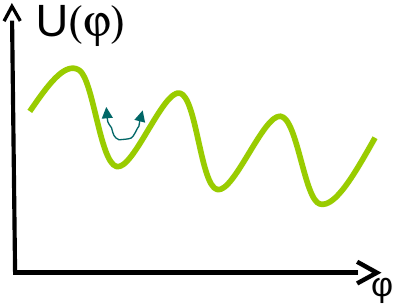
\includegraphics[width=0.4\textwidth]{immagini/washboard_potential.png}
\end{figure}
\hspace{-0.6cm}Interpretando il problema come quello di una particella in un potenziale, possiamo dire che la particella può rimanere confinata in uno dei minimi del potenziale, ottenendo così configurazioni stabili.\\
Se la particella si trova in un minimo con $\dot{\varphi}=0$, allora, per le relazioni di Josephson, non compare alcuna tensione e il sistema supporta una corrente priva di dissipazione.\\
Questa configurazione corrisponde al cosiddetto \emph{S-state}, cioè lo stato superconduttivo. Gli stati superconduttivi sono quindi configurazioni stabili del circuito che possono esistere soltanto se la corrente di bias è minore della corrente critica.\\
Per capire meglio la dinamica del sistema è utile studiare il comportamento del potenziale nelle vicinanze di un minimo $\varphi_m$. Sviluppando il coseno attorno a tale minimo otteniamo\mn{Questa cosa a me non convince per niente. Sviluppando in serie si dovrebbe ottenere
\begin{equation*}
    \cos{\varphi}
    \approx
    \cos{\varphi_m}
    -
    \frac{1}{2}
    \cos{\varphi_m}
    (\varphi-\varphi_m)^2
\end{equation*}
quindi comparirebbe un fattore $\cos{\varphi_m}$ che qui non appare. L'unica possibilità è che ci si stia mettendo nel limite di bias piccolo, cioè $I_x \ll I_c$, nel quale $\varphi_m \approx 2\pi m$ e quindi $\cos{\varphi_m}\approx1$.}
\begin{equation*}
    -E_J\cos{\varphi}
    \approx
    -E_J\cos{\varphi_m}
    +
    \frac{E_J}{2}
    (\varphi-\varphi_m)^2
\end{equation*}
Il potenziale risulta quindi approssimativamente parabolico nelle vicinanze del minimo. Il coefficiente del termine quadratico determina la frequenza delle piccole oscillazioni attorno al minimo, cioè la frequenza di plasma.\\
Come avviene per una particella ordinaria, tale frequenza dipende dalla massa efficace, che in questo caso è interpretata dalla capacità:
\begin{equation*}
    E_J
    =
    m\omega_p^2
    =
    C
    \qty(
        \frac{\hbar}{2e}
    )^2
    \omega_p^2
\end{equation*}
da cui
\begin{equation*}
    \omega_p
    =
    \sqrt{
        \frac{E_J}{C}
        \qty(
            \frac{2e}{\hbar}
        )^2
    }
    =
    \frac{\sqrt{2E_JE_C}}{\hbar}
\end{equation*}
Possiamo quindi interpretare la dinamica della giunzione, trascurando la dissipazione, come quella di una particella con energia fissata composta da contributi cinetici e potenziali.\\
Se la particella possiede energia sufficiente, può superare la barriera del potenziale e iniziare a ``rotolare'' lungo il washboard potential. In assenza di dissipazione questo moto persisterebbe indefinitamente; introducendo la resistenza, esso viene invece smorzato.\\
Vediamo ora che cosa accade quando la corrente di bias supera la corrente critica:
\begin{figure}[H]
    \centering
    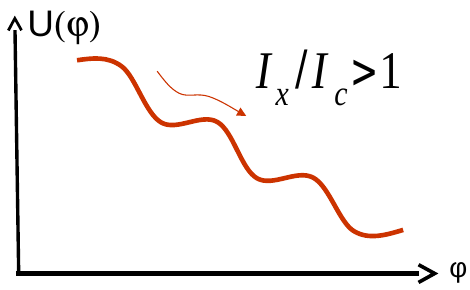
\includegraphics[width=0.4\textwidth]{immagini/washboard_potential_no_minima.png}
\end{figure}
\hspace{-0.6cm}In questo caso il potenziale non presenta più minimi, ma soltanto punti di flesso. Non esistono quindi configurazioni stabili e la condizione $\dot{\varphi}=0$ non può più essere soddisfatta.\\
Questo significa che compare necessariamente una tensione ai capi della giunzione. Inoltre, poiché nel circuito è presente una resistenza, la tensione genera anche una corrente dissipativa.\\
Per questo motivo, quando $I_x>I_c$, il sistema si trova nel cosiddetto \emph{R-state}, cioè nello stato resistivo, in contrapposizione allo stato superconduttivo.
\subsection{Caratteristica corrente--tensione}
Vogliamo adesso risolvere questa equazione nei due diversi regimi.\\
Cominciamo dal regime overdamped, cioè il regime in cui il fattore di qualità del circuito è minore di uno. Con fattore di qualità intendiamo la combinazione tra la frequenza di plasma delle oscillazioni attorno al minimo e la scala temporale del circuito determinata da $RC$,\mn{In altre parole, esso rappresenta il rapporto tra la scala temporale caratteristica del circuito la scala temporale delle oscillazioni attorno al minimo.} dal momento che stiamo considerando un circuito con comportamento sia resistivo che capacitivo.\\
Partiamo dall'equazione circuitale scritta in termini della fase:
\begin{equation*}
    I_x = C \frac{\hbar}{2e} \dv[2]{\varphi}{t} + \frac{\hbar}{2e} \frac{1}{R} \dv{\varphi}{t} + I_0 \sin{\varphi}
\end{equation*}
Dividendo per $I_c$ e ricordando che $\omega_p$ è data da
\begin{equation*}
    \omega_p=\qty(\frac{2eI_c}{\hbar C})^{\frac{1}{2}}
\end{equation*}
possiamo riscrivere tale equazione come
\begin{equation*}
    i_x = \frac{1}{\omega_p^2} \dv[2]{\varphi}{t} + \frac{1}{\omega^2_p} \frac{1}{R C} \dv{\varphi}{t} + \sin{\varphi}
\end{equation*}
Se adesso riscriviamo l'equazione in termini della quantità adimensionale $\tau=\omega_p t$, da cui $\dd{\tau}=\omega_p \dd{t}$ e $\dd[2]{\tau}=\omega_p^2 \dd[2]{\varphi}{t}$, otteniamo:
\begin{equation*}
    i_x = \dv[2]{\varphi}{\tau} + \frac{1}{Q} \dv{\varphi}{\tau} + \sin{\varphi}
\end{equation*}
dove
\begin{equation*}
    Q=\omega_p RC
\end{equation*}
è il fattore di qualità.\\
Se $Q \ll 1$, cioè se ci troviamo nel cosiddetto regime overdamped, il termine dissipativo domina rispetto alla derivata seconda della fase. Per capire quindi il comportamento del sistema possiamo limitarci all'equazione approssimata
\begin{equation*}
    i_x \approx \frac{1}{Q} \dv{\varphi}{\tau} + \sin{\varphi}
\end{equation*}
Questa equazione riproduce immediatamente il comportamento atteso per $I_x < I_c$, cioè la presenza di minimi del potenziale e quindi di stati stazionari.\sn{Infatti, per $I_x < I_c$ l'equazione ammette soluzioni statiche, nelle quali la fase assume un valore costante. Nel linguaggio del washboard potential ciò significa che esistono minimi del potenziale in cui la particella può fermarsi. In altre parole, se la corrente applicata è minore della corrente critica, la forza esercitata dalla corrente non è sufficiente a far "scivolare" la fase lungo il potenziale. La fase rimane intrappolata in un minimo e il sistema raggiunge un equilibrio stabile.}\\
A questo punto vogliamo trovare la relazione tra la corrente di bias applicata $I_x$ e la corrente che attraversa il circuito, espressa in forma adimensionale come $i=\frac{I}{I_c}$. Vogliamo inoltre derivare separatamente i contributi di corrente che attraversano la giunzione Josephson e la resistenza.\\
Nel regime $I_x<I_c$, la corrente scorre unicamente attraverso l'elemento Josephson e dipende dal valore della fase associato a uno dei minimi del potenziale. La dipendenza rispetto a $I_x$ risulta lineare: $i_J=i_x$\\
Nel grafico seguente dobbiamo quindi guardare soltanto la regione con $I_x<I_c$; la parte restante emergerà invece dal regime con $I_x>I_c$.
\begin{figure}[H]
    \centering
    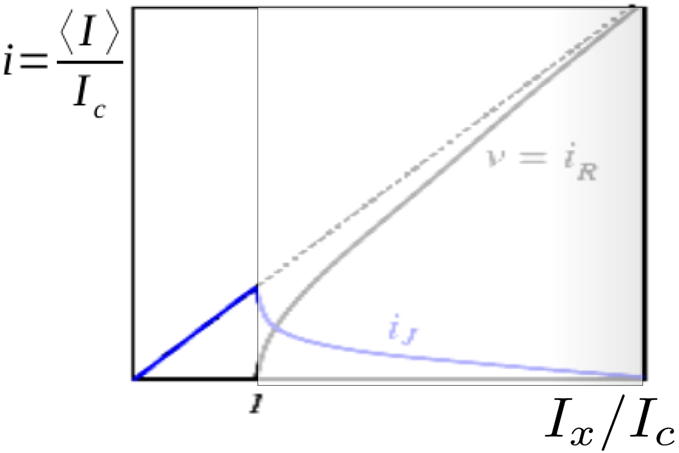
\includegraphics[width=0.5\textwidth]{immagini/IV_characteristic_RCSJ.png}
\end{figure}
\hspace{-0.6cm}Per trovare l'andamento per $I_x>I_c$, dobbiamo risolvere l'equazione. Riscriviamola come\sn{\cite{Tinkham} Se guardiamo la forma dell'equazione circuitale si vede che, per $I > I_{c}$, $\dv*{\varphi}{t}$ è sempre positivo, ma varia periodicamente con $\sin{\varphi}$. La fase avanza più lentamente (corrispondendo a una tensione istantanea più bassa) quando $\sin\varphi$ è positivo (così che la supercorrente sia nella direzione diretta), e viceversa quando $\sin\varphi$ è negativo e la supercorrente si oppone alla corrente continua di bias.}
\begin{equation*}
    \dv{\varphi}{\tau} = Q \qty( i_x-\sin{\varphi} )
\end{equation*}
Separando le variabili otteniamo
\begin{equation*}
    Q \dd{\tau} = \frac{\dd{\varphi}}{i_x-\sin{\varphi}}
\end{equation*}
Per trovare la tensione media temporale integriamo tale equazione per determinare il periodo di tempo $T$ richiesto affinché $\varphi$ aumenti di $2\pi$:
\begin{equation*}
    Q \int_{0}^{\tilde{T}} \dd{\tau} = \int_{0}^{2\pi} \frac{\dd{\varphi}}{i_x-\sin{\varphi}}
\end{equation*}
dove $\tilde{T}$ è il periodo in unità di $\omega_p$, quindi $\tilde{T}=\omega_p T$.\\
Si trova quindi\mn{Da notare che abbiamo usato il risultato noto
\begin{equation*}
    \int_{0}^{2\pi} \frac{\dd{\varphi}}{a-\sin{\varphi}}
    =
    \frac{2\pi}{\sqrt{a^2-1}}
    \quad\text{per } a>1
\end{equation*}}
\begin{equation*}
    Q\tilde{T} = \frac{2\pi}{\sqrt{i_x^2-1}}
\end{equation*}
Usando la definizione di $Q$, possiamo riscrivere questa relazione nella forma
\begin{equation*}
    \omega_p RC\,\tilde{T}
    =
    \frac{2\pi}{\sqrt{i_x^2-1}}
\end{equation*}
Invertendo la relazione otteniamo l'espressione del periodo delle oscillazioni:
\begin{equation}
    \tilde{T}
    =
    \frac{1}{\omega_p RC}
    \frac{2\pi}{\sqrt{i_x^2-1}}
    \label{eq:period_oscillations_RCSJ}
\end{equation}
Per procedere nello studio della corrente utilizziamo ora la seconda relazione di Josephson.\\
Nel limite overdamped la fase dipende dal tempo. Vogliamo quindi determinare il valor medio della fase e della corrente nei diversi elementi del circuito su un periodo caratteristico $\tilde{T}$.\\
Usiamo la relazione di Josephson
\begin{equation*}
    V
    =
    \frac{\hbar}{2e}
    \dot{\varphi}
\end{equation*}
e valutiamo il valor medio della tensione:
\begin{equation*}
    \expval*{V}
    = \frac{1}{\tilde{T}} \int_{0}^{\tilde{T}} V \dd{t}
    = \frac{\hbar}{2e} \frac{1}{\tilde{T}} \int_{0}^{\tilde{T}} \dd{t} \dot{\varphi}
    = \frac{\hbar}{2e} \expval*{\dot{\varphi}}
\end{equation*}
Quindi
\begin{equation*}
    \expval*{V} = \frac{\hbar}{2e} \expval*{\dot{\varphi}}
\end{equation*}
Se definiamo $\tilde{T}$ come il tempo necessario affinché la fase cambi di $2\pi$, possiamo approssimare
\[
\expval*{\dot{\varphi}}
\simeq
\frac{2\pi}{\tilde{T}},
\]
da cui
\begin{equation}
    \expval*{V}
    =
    \frac{\hbar}{e}
    \frac{\pi}{\tilde{T}}
    \label{eq:average_voltage_RCSJ}
\end{equation}
Sostituendo ora l'\eqrefcustom{eq:period_oscillations_RCSJ} nell'\eqrefcustom{eq:average_voltage_RCSJ} otteniamo
\begin{equation*}
    \expval*{V}=R\sqrt{I_x^2-I_c^2}
\end{equation*}
La corrente che attraversa la resistenza è quindi
\begin{equation*}
    I_R
    =\frac{\expval*{V}}{R}
    =\sqrt{I_x^2-I_c^2}
\end{equation*}
Usando infine la conservazione della corrente possiamo ricavare il valor medio della corrente Josephson:
\begin{equation*}
    \expval*{I_J}
    =I_c \expval*{\sin{\varphi}}
    =I_x-\sqrt{I_x^2 - I_c^2}
\end{equation*}
Osserviamo ora il comportamento dei diversi contributi di corrente, espressi in forma adimensionale (cioè divisi per $I_c$), in funzione della corrente di bias adimensionale $i_x$.
\begin{figure}[H]
    \centering
    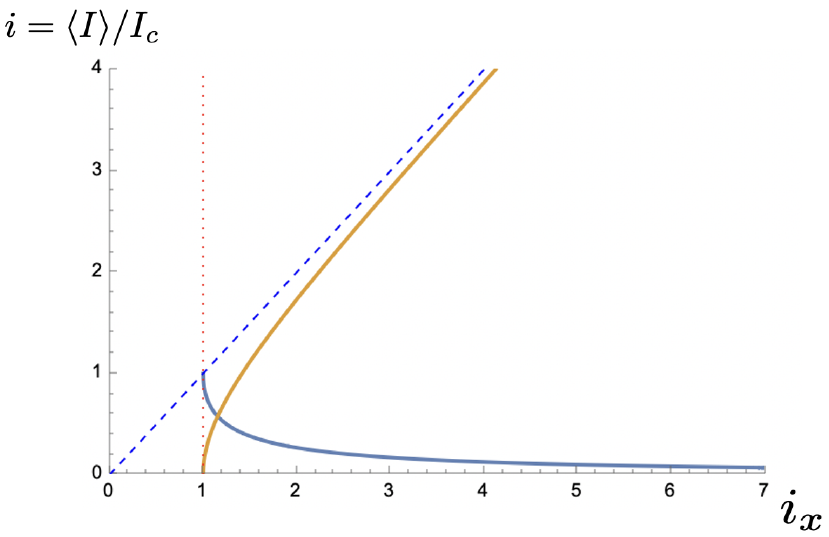
\includegraphics[width=0.5\textwidth]{immagini/current_phase_relation_RCSJ.png}
\end{figure}
\hspace{-0.6cm}Siamo nel regime $i_x>1$. La parte resistiva parte da zero per $i_x=1$ e poi cresce progressivamente. Quanto più aumenta la corrente di bias, tanto più questa relazione tende a diventare lineare.\\
La corrente Josephson, invece, parte da $1$ per $i_x=1$ e poi diminuisce come mostrato nella figura.\\
Riassumiamo quindi i due regimi discussi:
\begin{itemize}[leftmargin=0.5cm]
    \item Per $I_x<I_c$ abbiamo l'\emph{S-state}. In questo caso esistono minimi del potenziale in corrispondenza di
    \begin{equation*}
        \bar{\Phi}=\frac{\Phi_0}{2\pi}\arcsin{\qty(\frac{I_x}{I_c})}
    \end{equation*}
    Questo stato corrisponde a un equilibrio stabile e quindi realizza l'effetto Josephson DC.
    \item Per $I_x>I_c$ abbiamo invece l'\emph{R-state}, poiché compare una componente resistiva. In questo caso non esistono più minimi del potenziale e la particella ``rotola'' lungo il washboard potential. Si manifesta quindi l'effetto Josephson AC, essenzialmente perché $\dot{\varphi} \neq 0$.
\end{itemize}
Questi due regimi, determinati dal valore della corrente di bias, danno quindi luogo rispettivamente all'effetto Josephson DC e all'effetto Josephson AC.\\
Questa è infine la forma tipica della caratteristica corrente--tensione osservata sperimentalmente:
\begin{figure}[H]
    \centering
    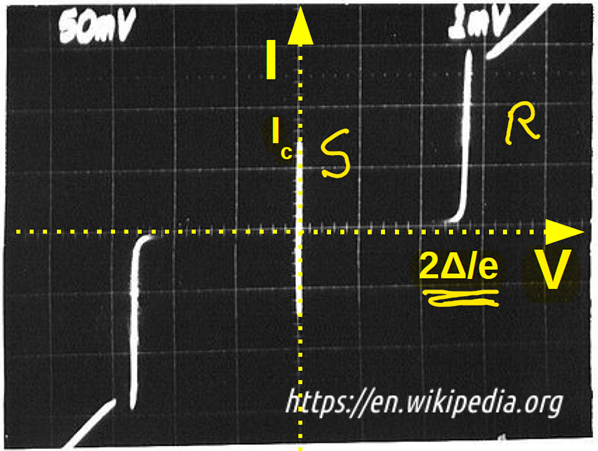
\includegraphics[width=0.5\textwidth]{immagini/IV_characteristic_experiment.png}
\end{figure}
\hspace{-0.6cm}Nel grafico è riportata la corrente in funzione della corrente di bias; equivalentemente possiamo reinterpretarlo come una caratteristica corrente--tensione.\\
Si osserva che:
\begin{itemize}[leftmargin=0.5cm]
    \item a tensione nulla compare lo stato superconduttivo (\emph{S-state});
    \item successivamente compare la parte resistiva.
\end{itemize}
La tensione alla quale compare la parte resistiva corrisponde alla condizione $V>\frac{2\Delta}{e}$, cioè quando l'energia fornita dalla tensione è sufficiente a rompere le coppie di Cooper.
\subsection{Lo stato R: retrapping e isteresi}
Consideriamo ancora la caratteristica corrente--tensione e cerchiamo di capire che cosa accade quando modifichiamo la corrente di bias applicata.
\begin{figure}[H]
    \centering
    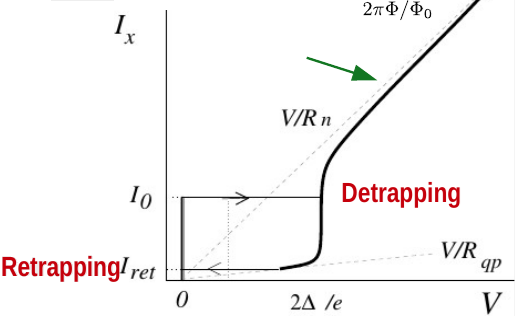
\includegraphics[width=0.6\textwidth]{immagini/IV_characteristic_experiment_2.png}
\end{figure}
\hspace{-0.6cm}Supponiamo di partire da uno stato resistivo, cioè dal regime in cui la particella sta ``rotolando'' lungo il potenziale, e immaginiamo ora di ridurre la corrente di bias, spostandoci a sinistra nel diagramma.\\
Per capire che cosa può accadere, torniamo all'analogia meccanica. Abbiamo una particella che sta scendendo lungo il potenziale e che quindi acquisisce energia cinetica. Ora incliniamo diversamente il potenziale, modificandone la forma in modo tale che compaiano nuovamente dei minimi.\\
Può allora succedere che, se la forma del potenziale viene modificata sufficientemente lentamente, la particella si trovi in un potenziale che possiede dei minimi ma abbia comunque energia cinetica sufficiente per superare le barriere tra un minimo e l'altro.\\
Che cosa significa questo nel grafico? Se partiamo da un certo valore della corrente di bias e poi la riduciamo, modifichiamo progressivamente la forma del washboard potential. Per un certo intervallo il sistema rimane nello stato resistivo, ma a un certo punto può accadere che l'energia acquisita dalla particella durante il moto sia maggiore di quella dissipata.\\
Quando questo accade, la particella può essere nuovamente catturata in uno dei minimi del potenziale e il sistema ritorna nello stato superconduttivo.\\
Se ora percorriamo il processo inverso, cioè partiamo dalla fase superconduttiva e aumentiamo la corrente di bias, può accadere che la particella ritorni nello stato resistivo seguendo però un percorso differente.\\
Si ottiene quindi quello che viene chiamato comportamento isteretico. In particolare:
\begin{itemize}[leftmargin=0.5cm]
    \item quando la corrente di bias viene ridotta si può avere un processo di \emph{retrapping}, nel quale il sistema passa dalla fase resistiva a quella superconduttiva;
    \item viceversa, aumentando la corrente di bias, il sistema può uscire dal minimo del potenziale e tornare nello stato resistivo, in un processo che viene talvolta chiamato \emph{detrapping}.\mn{Si parla di detrapping perché, nello stato resistivo, la particella non è più confinata in un minimo ma scivola lungo il potenziale.}
\end{itemize}
Questo è quindi il comportamento che si osserva in un circuito quando la corrente di bias viene fatta variare avanti e indietro.
\subsection{Comportamento induttivo}
Il passo successivo consiste nell'analizzare il circuito passando gradualmente da regimi in cui la fase si comporta come una variabile classica a regimi in cui essa mostra un comportamento quantistico.\\
Come abbiamo già discusso, in opportune condizioni possiamo quantizzare sia la differenza di fase tra i due lati della giunzione sia la carica presente sugli elettrodi, trattando queste quantità come variabili quantistiche. Questo è possibile perché esse soddisfano una relazione di indeterminazione che deriva originariamente dalla relazione di indeterminazione tra numero e fase del condensato superconduttivo.\\
Il punto importante è che, se la giunzione Josephson è sufficientemente piccola, possiamo entrare in un regime in cui emergono effetti quantistici associati sia alla fase sia alla carica. Si tratta di un comportamento che finora non abbiamo ancora descritto esplicitamente.\\
Per osservare questi effetti è necessario considerare giunzioni di dimensioni sufficientemente ridotte, come avevamo già anticipato. Inoltre vedremo che tali fenomeni compaiono anche in geometrie differenti, incluse configurazioni ad anello nelle quali la fase è direttamente collegata al flusso magnetico.\\
Questa osservazione serve a giustificare il motivo per cui vogliamo ora descrivere il comportamento induttivo della giunzione. Nei circuiti che considereremo comparirà infatti un'induttanza che include anche il contributo della giunzione Josephson stessa, e tale contributo sarà non lineare, come vedremo tra poco. Il passo successivo sarà poi ricavare la forma esplicita delle variabili quantistiche che descrivono l'elemento Josephson all'interno del circuito.\\
Cominciamo considerando una giunzione Josephson nel regime di piccole oscillazioni attorno a un minimo del potenziale.\\
Esprimendo $\varphi$ in termini del flusso magnetico $\Phi$, nel caso di una giunzione inserita in un circuito, il potenziale per un sistema non polarizzato ($I_x=0$) è
\begin{equation*}
    U(\Phi)
    \approx
    -E_J
    \qty[
        1
        -
        \frac{1}{2}
        \qty(
            \frac{2\pi\Phi}{\Phi_0}
        )^2
    ]
    =
    -E_J
    +
    \frac{\Phi^2}{2L_J}
\end{equation*}
dove abbiamo sviluppato il coseno attorno al minimo $\bar{\varphi}=0$.\\
Questa espressione ci permette di identificare immediatamente l'induttanza della giunzione, che è una quantità che avevamo già introdotto in precedenza.\\
Consideriamo ora il caso $0\leq I_x<I_0$. Se sviluppiamo il potenziale attorno a uno dei minimi $\varphi_m\neq0$, corrispondente a un valore del flusso $\bar{\Phi}$, otteniamo
\begin{equation*}
    \begin{split}
        U(\Phi)
        \approx\;
        &U(\bar{\Phi})
        +
        \frac{(\Phi-\bar{\Phi})^2}{2}
        \qty[
            \qty(
                \frac{2\pi}{\Phi_0}
            )^2
            E_J
            \cos{
                \qty(
                    \frac{2\pi\bar{\Phi}}{\Phi_0}
                )
            }
        ]
        \\
        =\;
        &U(\bar{\Phi})
        +
        \frac{(\Phi-\bar{\Phi})^2}{2L_J(I_x)}.
    \end{split}
\end{equation*}
Rispetto al caso precedente compare quindi un termine aggiuntivo nello sviluppo di Taylor, che dipende esplicitamente dalla posizione del minimo.\\
Questo significa che l'induttanza dipende dalla corrente applicata, perché il valore di $\bar{\Phi}$ è legato al minimo $\varphi_m$, e tali minimi dipendono direttamente dalla corrente di bias. In altre parole, se consideriamo il washboard potential e sviluppiamo il potenziale attorno a uno dei suoi minimi, otteniamo un'induttanza differente per ciascun minimo.\\
Questo non è sorprendente, perché stiamo considerando configurazioni fisicamente diverse del sistema, determinate dal valore della corrente di bias che inclina il potenziale.\\
Possiamo quindi descrivere l'elemento Josephson come un elemento la cui induttanza dipende dalla corrente di bias:
\begin{equation*}
    L_J(I_x)
    =
    L_J
    \qty[
        1-
        \qty(
            \frac{I_x}{I_0}
        )^2
    ]^{-1/2}
\end{equation*}
La corrente di bias modifica anche la frequenza di plasma, cosa che risulta naturale perché stiamo considerando oscillazioni attorno a minimi differenti:
\begin{equation*}
    \omega_p(I_x)=\omega_p \qty[ 1- \qty( \frac{I_x}{I_0} )^2]^{1/4}
\end{equation*}
Dobbiamo quindi tenere presente che, variando la corrente di bias, possiamo ottenere differenti valori dell'induttanza Josephson.\\
Questo comportamento non riguarda soltanto configurazioni ad anello, ma vale più in generale per circuiti contenenti giunzioni Josephson, poiché deriva direttamente dalla struttura del washboard potential.
\subsection{Lagrangiana/Hamiltoniana di una giunzione ideale}
Facciamo ora il passo che ci conduce alla quantizzazione del sistema.\\
Consideriamo il modello RCSJ e scriviamo l'equazione in funzione del flusso (che in questo caso rappresenta il flusso del circuito e non necessariamente quello della sola giunzione):
\begin{equation*}
    I_x
    =
    C\ddot{\Phi}
    +
    \frac{\dot{\Phi}}{R}
    +
    I_0
    \sin{
        \qty(
            \frac{2\pi\Phi}{\Phi_0}
        )
    }
\end{equation*}
Se consideriamo il limite underdamped, in cui la resistenza tende all'infinito, possiamo trascurare il termine dissipativo e otteniamo
\begin{equation*}
    I_x
    =
    C\ddot{\Phi}
    +
    I_0
    \sin{
        \qty(
            \frac{2\pi\Phi}{\Phi_0}
        )
    }
\end{equation*}
Vediamo quindi che abbiamo un'equazione equivalente a quella di una particella di massa $C$ che si muove in un potenziale. Possiamo dunque utilizzare gli strumenti della meccanica classica: scrivere una lagrangiana, ricavare da essa l'hamiltoniana e infine quantizzare il sistema imponendo opportune relazioni di commutazione.\\
In questo caso è immediato verificare che l'equazione circuitale senza dissipazione deriva dalla lagrangiana
\begin{equation*}
    \mathcal{L}
    =
    \frac{C}{2}\dot{\Phi}^2
    -
    U(\Phi)
\end{equation*}
dove compare un termine cinetico meno un'energia potenziale, con
\begin{equation*}
    U(\Phi)
    =
    -
    E_J
    \cos{
        \qty(
            \frac{2\pi\Phi}{\Phi_0}
        )
    }
    -
    I_x\Phi.
\end{equation*}
Possiamo ora ricavare il momento coniugato derivando la lagrangiana rispetto alla velocità:
\begin{equation*}
    \pdv{\mathcal{L}}{\dot{\Phi}}
    =
    C\dot{\Phi}
    =
    C(V_L-V_R)
    =
    Q
\end{equation*}
dove abbiamo utilizzato il fatto che $\dot{\Phi}$ può essere espresso in termini della differenza di potenziale ai capi della giunzione. Questa quantità non è altro che la carica della giunzione.\\
Possiamo quindi scrivere l'hamiltoniana:
\begin{equation*}
    \mathcal{H}(Q;\Phi)
    =
    \dot{\Phi}
    \pdv{\mathcal{L}}{\dot{\Phi}}
    -
    \mathcal{L}
    =
    \frac{Q^2}{2C}
    +
    U(\Phi).
\end{equation*}
In particolare, il primo termine rappresenta l'energia elettrostatica. Definendo infatti $q=\frac{Q}{2e}$, esso può essere riscritto come $E_C q^2$.\\
Il motivo per cui introduciamo tutti questi passaggi è che vogliamo costruire un formalismo generale utilizzabile per descrivere circuiti contenenti differenti elementi e differenti geometrie. In circuiti più complessi possono infatti comparire vincoli circuitali e non è immediato identificare le variabili canoniche coniugate.\\
Quello che faremo ora è quindi procedere verso la descrizione quantistica dei circuiti.\\
La manifestazione più tipica del comportamento quantistico di un sistema è la presenza di livelli energetici discreti. La domanda è quindi se sia possibile osservare un comportamento quantistico in un circuito contenente una giunzione Josephson, cioè avere evidenza sperimentale di livelli energetici discreti del circuito. La risposta è naturalmente sì, ma vediamo come.\\
Consideriamo la giunzione nel regime underdamped e nello stato S. Abbiamo già visto che l'energia della giunzione è data dalla somma dell'energia di carica e dell'energia Josephson:
\begin{equation*}
    \mathcal{H}
    =
    \frac{Q^2}{2C}
    -
    E_J
    \cos{
        \qty(
            \frac{2\pi\Phi}{\Phi_0}
        )
    }.
\end{equation*}
Abbiamo inoltre detto che queste variabili possono essere quantizzate.\\
Per capire se il comportamento del sistema sia quantistico oppure no, e in quali condizioni gli effetti quantistici diventino osservabili, possiamo approssimare il potenziale cosinusoidale tramite una successione di pozzi armonici.\\
In questo caso la scala energetica caratteristica è fissata dalla frequenza delle piccole oscillazioni attorno al minimo, cioè
\begin{equation*}
    \hbar\omega_p
    =
    \sqrt{2E_JE_C}
\end{equation*}
Poiché in questo caso non abbiamo corrente di bias, tutti i minimi sono equivalenti e compare semplicemente la frequenza di plasma che abbiamo già introdotto.\\
Se interpretiamo il sistema come una particella classica in un potenziale armonico, abbiamo che:
\begin{itemize}[leftmargin=0.5cm]
    \item la coordinata della particella è la fase;
    \item la quantità analoga all'impulso è la carica;
    \item la massa è sostituita dalla capacità;
    \item la frequenza caratteristica è la frequenza delle piccole oscillazioni attorno al minimo.
\end{itemize}
Otteniamo un comportamento essenzialmente classico quando l'energia di carica è sufficientemente piccola, cioè quando la ``massa efficace'' è grande. In questa situazione la frequenza di plasma è molto minore di $E_J$.\\
Entriamo invece nel regime quantistico quando queste condizioni non sono più soddisfatte e quando la temperatura è sufficientemente bassa rispetto all'energia quantistica delle oscillazioni:
\begin{equation*}
    k_BT
    \ll
    \hbar\omega_p
\end{equation*}
Abbiamo già discusso gli ordini di grandezza tipici dei parametri di una giunzione Josephson. In particolare abbiamo visto che, per giunzioni grandi, osservare effetti quantistici richiederebbe non soltanto temperature estremamente basse, ma anche energie Josephson molto piccole, il che implica barriere molto grandi e quindi giunzioni molto piccole.\\
Per questo motivo, nelle grandi giunzioni Josephson non si osservano effetti di coerenza quantistica, mentre nelle piccole giunzioni tali effetti possono emergere. In questo caso possiamo sperare di osservare la discrezione dei livelli energetici all'interno del potenziale, cioè la presenza di stati quantizzati distinti.\\
Questo effetto è stato osservato sperimentalmente per la prima volta nel 1985. Il circuito utilizzato era una giunzione Josephson in una configurazione che oggi chiameremmo \emph{phase qubit}. In questo caso il potenziale non è semplicemente il coseno periodico, ma assume una forma inclinata con un pozzo metastabile:
\begin{figure}[H]
    \centering
    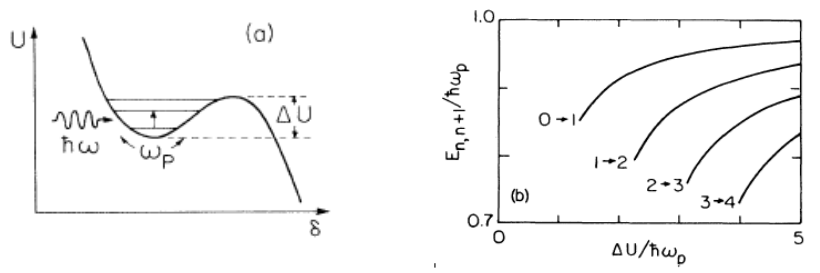
\includegraphics[width=0.9\textwidth]{immagini/potential_phase_qubit.png}
\end{figure}
\hspace{-0.6cm}Se il pozzo di potenziale è sufficientemente profondo, esso può supportare livelli energetici discreti.\\
Vediamo cosa si può fare sperimentalmente. Interpretiamo ancora il problema in termini di particella classica. Se la temperatura è sufficientemente bassa, ad esempio idealmente nulla, la particella rimane nello stato fondamentale.\\
Se ora irradiamo il sistema con una radiazione la cui frequenza è risonante con la prima transizione energetica, può avvenire una transizione verso il primo stato eccitato.\\
Se la particella si trova in uno stato eccitato sufficientemente vicino alla cima della barriera, allora la probabilità di tunneling attraverso la barriera aumenta, perché la barriera effettiva risulta più sottile rispetto a quella vista dallo stato fondamentale.\\
Se questo processo avviene, la coordinata cambia improvvisamente passando dal minimo del potenziale a un valore differente. Di conseguenza compare una derivata temporale della fase diversa da zero:
\[
\dot{\varphi}\neq0.
\]
Ma questo implica immediatamente la comparsa di una tensione ai capi della giunzione. L'evidenza sperimentale del tunneling attraverso la barriera consiste quindi proprio nell'osservazione di una caduta di tensione sulla giunzione.\\
Nel famoso esperimento del 1985 si irradiava il sistema con frequenze differenti, risonanti con differenti transizioni del pozzo di potenziale. Ad esempio, scegliendo una frequenza risonante con la transizione $0\to1$, compariva un picco di corrente associato all'eccitazione del sistema.\\
Ripetendo l'esperimento con frequenze differenti, fu possibile osservare anche le transizioni $1\to2$, eccetera. Inoltre la larghezza della barriera veniva modificata sperimentalmente:
\begin{itemize}[leftmargin=0.5cm]
    \item con una barriera molto piccola era possibile osservare soltanto i primi livelli;
    \item aumentando la barriera diventavano accessibili livelli più elevati, purché la frequenza della radiazione fosse risonante con la corrispondente differenza energetica.
\end{itemize}
Questo esperimento rappresentò la prima osservazione della discrezione dei livelli energetici in un circuito basato su una giunzione Josephson.\\
La descrizione in termini di particella in un potenziale è molto intuitiva, ma bisogna ricordare che il circuito deriva da un sistema superconduttivo. Le transizioni osservate coinvolgono quindi un enorme numero di elettroni, poiché la fase è la differenza di fase tra due condensati superconduttivi.\\
I livelli discreti che osserviamo nel potenziale dipendono dunque da variabili collettive macroscopiche, ed è proprio questa struttura che costituisce la base dell'utilizzo di questi circuiti per realizzare dispositivi quantistici.\\
In pratica, ciò che viene sfruttato è la quantizzazione dei livelli energetici per implementare operazioni che coinvolgono, ad esempio, due livelli del sistema.\\
Con il termine ``operazione'' intendiamo qualcosa di analogo alle operazioni logiche di un computer classico, dove due livelli del circuito giocano il ruolo degli stati $0$ e $1$. La differenza fondamentale è che qui i due livelli sono autostati di un'hamiltoniana quantistica del circuito.\\
I parametri che determinano tale hamiltoniana includono:
\begin{itemize}[leftmargin=0.5cm]
    \item la corrente critica della giunzione;
    \item la capacità della giunzione;
    \item la temperatura;
    \item la corrente di bias applicata;
    \item il campo magnetico, che impone un flusso magnetico.
\end{itemize}
Abbiamo quindi diversi parametri controllabili, sia di natura elettrostatica sia legati direttamente alla realizzazione fisica della giunzione, che possono essere utilizzati per manipolare l'evoluzione dei livelli energetici del circuito quantistico.
\section{Computazione: evoluzione controllata di un sistema fisico (computer)}
Cominciamo a discutere il possibile utilizzo dei sistemi superconduttivi basati sull'effetto Josephson come elementi fondamentali per il calcolo quantistico.
\subsection{Dal bit classico al qubit}
Vediamo innanzitutto l'idea di base che sta dietro al computer quantistico. In un computer classico abbiamo:
\begin{itemize}[leftmargin=0.5cm]
    \item una codifica dell'informazione tramite bit classici;
    \item un'unità di elaborazione (CPU) nella quale l'informazione evolve.
\end{itemize}
L'informazione è quindi codificata in una stringa di $0$ e $1$, che tipicamente corrispondono ai due stati stabili di un circuito classico, e viene poi elaborata tramite l'elettronica del sistema.\\
L'idea del calcolo quantistico consiste invece nel codificare ed elaborare l'informazione utilizzando sistemi quantistici. Questo modifica completamente le regole della computazione.\\
L'idea generale è schematizzata nella figura seguente:
\begin{figure}[H]
    \centering
    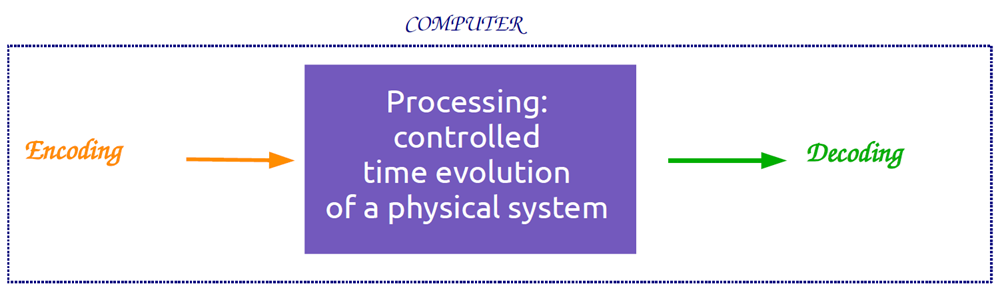
\includegraphics[width=0.8\textwidth]{immagini/computation.png}
\end{figure}
\hspace{-0.6cm}Per un sistema classico l'informazione è codificata in un bit classico (\emph{bit} sta per \emph{binary digit}), che corrisponde tipicamente ai due stati stabili di un circuito classico, ad esempio un circuito elettrico in cui la corrente può fluire oppure no.\\
Se vogliamo interpretare questi due stati come stati di un sistema classico, possiamo immaginarli come i due stati localizzati di una particella in un potenziale a doppio pozzo.
\begin{figure}[H]
    \centering
    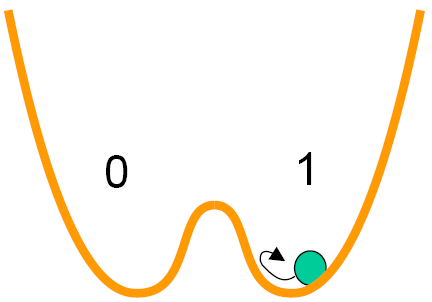
\includegraphics[width=0.4\textwidth]{immagini/double_well_potential_classical.png}
\end{figure}
\hspace{-0.6cm}Supponiamo quindi che i due stati logici derivino dai due stati classici corrispondenti a una particella localizzata in uno dei due minimi del potenziale. Questa è la descrizione tipica di un bit classico.\\
Nel caso quantistico, invece, l'informazione è codificata in un \emph{qubit} (\emph{quantum bit}). L'idea è quindi quella di utilizzare un sistema con due stati quantistici stabili.\\
Se consideriamo ancora il caso del doppio pozzo, sappiamo immediatamente dalla meccanica quantistica quale sia la differenza rispetto al caso classico.
\begin{figure}[H]
    \centering
    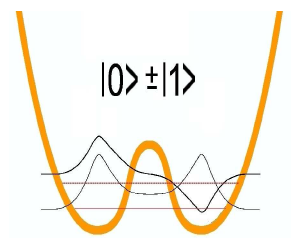
\includegraphics[width=0.35\textwidth]{immagini/double_well_potential_quantum.png}
\end{figure}
\hspace{-0.6cm}Se il sistema è quantistico ed è descritto da un potenziale a doppio pozzo, i due autostati a più bassa energia, indicati con $\ket{0}$ e $\ket{1}$, non corrispondono a stati localizzati nei due minimi, bensì a stati delocalizzati:
\begin{itemize}[leftmargin=0.5cm]
    \item uno con funzione d'onda simmetrica (lo stato fondamentale);
    \item uno con funzione d'onda antisimmetrica.
\end{itemize}
Poiché questi sono stati quantistici, il sistema può trovarsi in una qualsiasi loro combinazione lineare:
\begin{equation*}
    \ket{\psi}
    =
    \alpha \ket{0}
    +
    \beta \ket{1}
\end{equation*}
grazie al principio di sovrapposizione.\\
L'idea dei blocchi fondamentali del calcolo quantistico è quindi analoga a quella del caso classico:
\begin{itemize}[leftmargin=0.5cm]
    \item abbiamo uno stato iniziale in cui l'informazione è codificata, in generale in una sovrapposizione;
    \item abbiamo una \emph{quantum processing unit}, cioè un sistema che evolve quantisticamente. L'evoluzione dello stato segue quindi la dinamica quantistica ed è descritta da un operatore unitario $U(t)$;
    \item l'output della computazione è data dallo stato evoluto:
    \begin{equation*}
        \ket{\psi}_{\rm out}
        =
        \alpha U(t)\ket{0}
        +
        \beta U(t)\ket{1}
    \end{equation*}
\end{itemize}
Sia all'ingresso sia all'uscita abbiamo quindi, in generale, una sovrapposizione di stati.\\
Il fatto che l'evoluzione sia unitaria implica che il dispositivo elabora simultaneamente l'informazione codificata in $\ket{0}$ e in $\ket{1}$. Questo è ciò che prende il nome di \emph{parallelismo quantistico}: la possibilità di operare in parallelo sui due stati di ingresso.\\
Questa è la differenza fondamentale rispetto al caso classico. In un computer classico, infatti, l'ingresso è o $0$ oppure $1$. Se vogliamo elaborare entrambe le informazioni dobbiamo eseguire il processo due volte, una volta preparando il sistema nello stato $0$ e una seconda volta preparando il sistema nello stato $1$.\\
Con un qubit, invece, entrambe le evoluzioni avvengono simultaneamente in un unico processo.\\
Questo vantaggio può sembrare limitato se pensiamo ad un singolo qubit, ma diventa enorme quando consideriamo un gran numero di qubit. Infatti, se abbiamo $N$ qubit, il numero di configurazioni possibili cresce come $2^N$.\\
Il parallelismo quantistico permette quindi di elaborare simultaneamente tutte le informazioni codificate in questo enorme spazio di stati.\\
Tuttavia, questo non è ancora l'aspetto più importante del vantaggio quantistico. Il vero vantaggio del calcolo quantistico emerge soprattutto quando consideriamo sistemi composti da molti qubit ed entra in gioco il concetto di entanglement. L'entanglement consiste nella possibilità di avere stati quantistici di sistemi composti che non sono fattorizzabili nei singoli sottosistemi. In altre parole, possiamo avere stati di più qubit che non possono essere descritti come semplici prodotti degli stati dei singoli qubit.\\
È proprio grazie alla possibilità di creare stati entangled che si possono sviluppare:
\begin{itemize}[leftmargin=0.5cm]
    \item algoritmi quantistici;
    \item protocolli di comunicazione quantistica;
    \item protocolli di crittografia quantistica.
\end{itemize}
Il vantaggio di questi protocolli deriva precisamente dall'entanglement e dalla possibilità di manipolare stati collettivi non fattorizzabili.\\
Le motivazioni profonde e tutte le implicazioni di questi aspetti vanno oltre gli obiettivi del corso.\\
Quello che ci interessa qui è discutere le implementazioni superconduttive dei qubit. La piattaforma superconduttiva presenta infatti numerosi vantaggi pratici e teorici ed è oggi una delle piattaforme più promettenti per la realizzazione di bit quantistici e per l'implementazione del calcolo quantistico.
\subsection{Implementazioni attuali dei qubit}
Diamo ora una panoramica generale delle diverse piattaforme attualmente investigate per l'implementazione dei qubit. Come possiamo vedere, esiste una notevole varietà di approcci.
\begin{figure}[H]
    \centering
    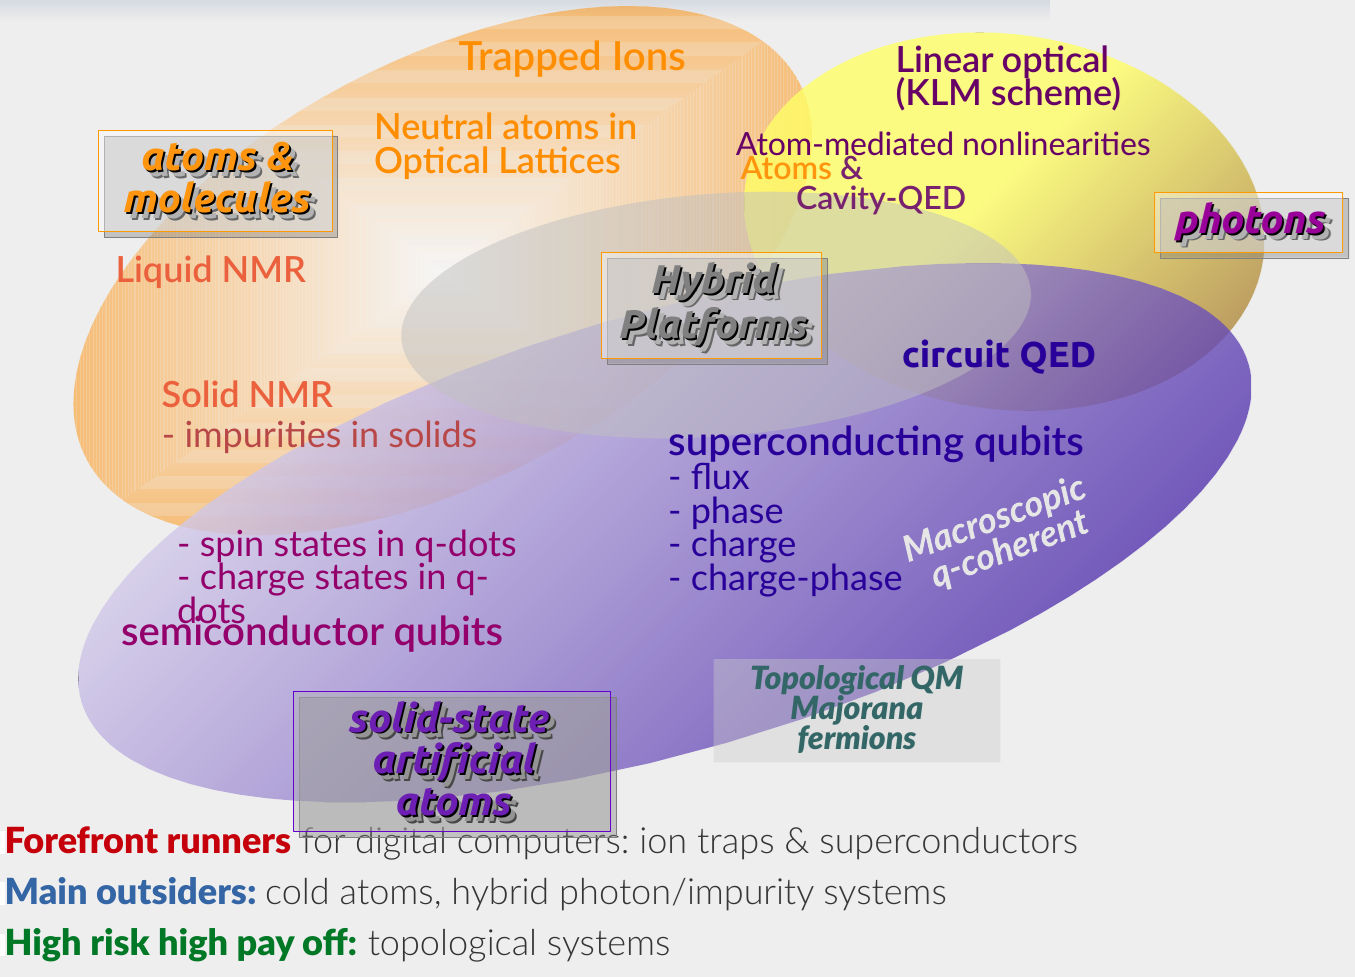
\includegraphics[width=0.8\textwidth]{immagini/quantum_computing_platforms.png}
\end{figure}
\hspace{-0.6cm}I qubit superconduttivi appartengono alla cosiddetta piattaforma \emph{solid state}, e la parola chiave associata a questa piattaforma è \emph{macroscopic quantum coherence}. Abbiamo già utilizzato questi termini per descrivere lo stato BCS di un superconduttore, ed è proprio questo l'ingrediente fondamentale su cui si basano i qubit superconduttivi.\\
Naturalmente non esistono soltanto i qubit superconduttivi. Esistono anche qubit semiconduttivi, che sono essenzialmente di due tipi:
\begin{itemize}[leftmargin=0.5cm]
    \item qubit basati sul grado di libertà di spin;
    \item qubit basati sul grado di libertà di carica.
\end{itemize}
Questi sistemi sono realizzati utilizzando singoli elettroni confinati in \emph{quantum dots} implementati in eterostrutture semiconduttive.\\
L'idea di base è che quanto più piccolo è il quantum dot, tanto più confinato è il potenziale e quindi tanto più discreti e non equidistanti diventano i livelli energetici.\\
L'ingrediente fondamentale è quindi che, in queste eterostrutture artificiali, possiamo creare un potenziale capace di localizzare particelle o elettroni. In tali condizioni possiamo ottenere sistemi a due livelli sufficientemente isolati dagli altri livelli energetici.\\
L'idea generale, indipendentemente dal dispositivo specifico, è quella di avere livelli energetici non equidistanti e utilizzare i due livelli a più bassa energia come qubit.\\
Se il confinamento deriva da un quantum dot, i livelli più bassi possono essere occupati da un elettrone. In questo caso si può:
\begin{itemize}[leftmargin=0.5cm]
    \item utilizzare la carica dell'elettrone (\emph{charge quantum dot});
    \item utilizzare i due stati di spin dell'elettrone come qubit.
\end{itemize}
Oltre a queste piattaforme esistono anche piattaforme più esotiche, ad esempio quelle basate sui fermioni di Majorana.\\
Esistono inoltre piattaforme atomiche e molecolari. Un esempio importante è quello degli atomi neutri intrappolati in reticoli ottici.\\
In questo caso l'idea è utilizzare i sistemi quantistici più semplici possibili, cioè gli atomi, che possiedono naturalmente livelli energetici discreti. Se tali livelli non sono equidistanti, possiamo pensare di utilizzare due livelli atomici come qubit.\\
È chiaro però che, sebbene sia relativamente semplice identificare due livelli atomici, la vera difficoltà consiste nel manipolarli.\\
Infatti, l'obiettivo finale è costruire un oggetto che possa essere utilizzato in maniera analoga ai bit classici:
\begin{itemize}[leftmargin=0.5cm]
    \item dobbiamo manipolare gli stati;
    \item leggere gli stati;
    \item realizzare operazioni logiche;
    \item controllarne l'evoluzione.
\end{itemize}
Fare tutto questo utilizzando singoli atomi è molto più complicato rispetto a una piattaforma a stato solido, dove i livelli quantistici emergono da dispositivi artificiali più facilmente controllabili e manipolabili.\\
Possiamo poi citare anche i fotoni. Anche i fotoni possono essere utilizzati come implementazioni di qubit.\\
A prima vista questo potrebbe sembrare sorprendente, ma bisogna ricordare che i fotoni possiedono un grado di libertà di polarizzazione.\\
Possiamo quindi codificare un sistema a due livelli nella polarizzazione di un singolo fotone propagante lungo un determinato cammino.\\
Un'altra possibilità consiste nel codificare l'informazione nella direzione di propagazione del fotone stesso.\\
I fotoni hanno inoltre il vantaggio di poter essere controllati e manipolati relativamente facilmente, e soprattutto risultano estremamente utili per la comunicazione quantistica grazie alla loro capacità di propagarsi su lunghe distanze, a differenza di oggetti localizzati.\\
Nel seguito ci concentreremo sui dispositivi basati sulla piattaforma superconduttiva.\\
L'elemento fondamentale di questa piattaforma è la giunzione Josephson, perché abbiamo visto che essa:
\begin{itemize}[leftmargin=0.5cm]
    \item è un elemento non lineare;
    \item presenta un comportamento quantistico.
\end{itemize}
Vedremo infatti come questo elemento costituisca il blocco fondamentale per realizzare quelli che vengono spesso chiamati \emph{atomi artificiali macroscopici unidimensionali}.\\
Mostreremo cioè come, utilizzando elementi Josephson, sia possibile fabbricare sistemi a due livelli tunabili, e la possibilità di controllare e modificare i parametri del sistema è un ingrediente cruciale.\\
I due effetti fondamentali che utilizzeremo sono:
\begin{itemize}[leftmargin=0.5cm]
    \item gli effetti di carica. Abbiamo visto che una giunzione Josephson possiede anche un'energia di carica associata al fatto che possiamo isolare un'isola superconduttiva e controllarne la carica. Esiste quindi un costo elettrostatico associato al fatto di caricare oppure no l'isola;
    \item l'effetto Josephson.
\end{itemize}
Vedremo che questi due ingredienti corrispondono a due scale energetiche fondamentali:
\begin{itemize}[leftmargin=0.5cm]
    \item l'energia di carica;
    \item l'energia Josephson.
\end{itemize}
\section{Phase qubit}
Il primo qubit che consideriamo è il cosiddetto phase qubit. Lo introduciamo per primo perché, tra quelli che analizzeremo, è il più semplice alla luce di quanto abbiamo già discusso.\\
Esso consiste essenzialmente in una giunzione Josephson polarizzata in corrente.\\
Abbiamo già ricavato l'hamiltoniana di questo dispositivo. La procedura generale è la seguente:
\begin{itemize}[leftmargin=0.5cm]
    \item si parte dalla descrizione classica del circuito;
    \item si quantizzano carica e fase trattandole come variabili canoniche coniugate;
    \item si costruisce l'hamiltoniana quantistica del circuito.
\end{itemize}
Seguendo questi passaggi otteniamo:
\begin{equation*}
    \hat{\mathcal{H}}
    =
    \frac{\hat{Q}^2}{2C}
    -
    E_J
    \cos{
        \biggl(
            \frac{2\pi\hat{\Phi}}{\Phi_0}
        \biggr)
    }
    -
    I_x\hat{\Phi}
\end{equation*}
che contiene:
\begin{itemize}[leftmargin=0.5cm]
    \item una parte elettrostatica;
    \item una parte Josephson.
\end{itemize}
In questo caso la parte Josephson è espressa in termini del flusso magnetico anziché direttamente della fase, poiché la giunzione è inserita in un circuito ad anello. Inoltre compare un termine aggiuntivo dovuto alla corrente di bias.\\
Abbiamo già visto che il contributo della corrente di bias, sommato all'energia Josephson, genera un potenziale di tipo washboard. Qui ci concentreremo semplicemente su uno dei minimi di questo potenziale.
\begin{figure}[H]
    \centering
    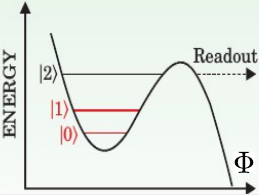
\includegraphics[width=0.5\textwidth]{immagini/washboard_potential_phase_qubit.png}
\end{figure}
\hspace{-0.6cm}L'idea è considerare gli autolivelli energetici all'interno di uno di questi pozzi di potenziale.\\
Se il pozzo è sufficientemente profondo, esso supporta un certo numero di livelli discreti. In particolare ci basta che siano presenti almeno tre livelli:
\begin{itemize}[leftmargin=0.5cm]
    \item i due livelli a energia più bassa, che identificheremo con gli stati $\ket{0}$ e $\ket{1}$;
    \item il terzo livello $\ket{2}$, che vedremo essere importante per il processo di readout.
\end{itemize}
Vediamo ora come emergono questi livelli a partire dall'hamiltoniana del sistema, analizzando in particolare l'energia potenziale.\\
Quello che facciamo è espandere il potenziale attorno a uno dei minimi del washboard potential:
\begin{equation*}
    U(\hat{\Phi})
    \approx
    U(\bar{\Phi})
    +
    \frac{\delta\hat{\Phi}^2}{2L_{Jx}}
    -
    \frac{\lambda_x}{6}
    \delta\hat{\Phi}^3
\end{equation*}
dove abbiamo definito
\[
\delta\hat{\Phi}
=
\hat{\Phi}-\bar{\Phi},
\]
cioè la deviazione del flusso rispetto alla posizione del minimo.\\
Abbiamo inoltre introdotto:
\begin{itemize}[leftmargin=0.5cm]
    \item $L_{Jx}$, cioè l'induttanza efficace della giunzione;
    \item $\lambda_x$, coefficiente associato al termine cubico nello sviluppo del potenziale.
\end{itemize}
Il pedice $x$ serve a ricordare che tale induttanza dipende dalla corrente di bias $I_x$. Infatti nello sviluppo del potenziale compare la derivata seconda valutata nel minimo $\bar{\Phi}$, e la posizione del minimo dipende proprio dalla corrente applicata.\\
Se osserviamo i primi due termini dello sviluppo, riconosciamo immediatamente un oscillatore armonico.\\
Possiamo quindi utilizzare la rappresentazione in seconda quantizzazione dell'oscillatore armonico e riscrivere l'hamiltoniana come
\begin{equation*}
    \hat{\mathcal{H}}
    =
    \hbar\omega_{px}
    \qty(
        \hat{a}^\dagger\hat{a}
        +
        \frac{1}{2}
    )
    -
    \frac{\lambda_x}{6}
    \delta\hat{\Phi}^3
\end{equation*}
dove $\omega_{px}$ è la frequenza delle piccole oscillazioni attorno al minimo.\\
L'idea è quindi trattare il termine non armonico, cioè il termine cubico, come una perturbazione.\\
Applicando la teoria perturbativa otteniamo livelli energetici del tipo
\begin{equation*}
    \varepsilon_n
    =
    \hbar\omega_{px}
    \qty(
        n+\frac{1}{2}
    )
    -
    \frac{\lambda_x}{6}
    \mel*{n}{\delta\hat{\Phi}^3}{n}
    +
    \frac{\lambda_x^2}{36}
    \sum_{m\neq n}
    \frac{ \bigl| \hspace{-0.1cm} \mel*{m}{\delta\hat{\Phi}^3}{n} \hspace{-0.1cm} \bigr|^2}{(n-m)\hbar\omega_{px}}
\end{equation*}
Abbiamo quindi sia il contributo armonico usuale che una correzione perturbativa dovuta all'anarmonicità del potenziale. In particolare stiamo considerando sia il primo sia il secondo ordine della teoria perturbativa.\\
Di conseguenza anche gli autostati vengono modificati:
\begin{equation*}
    \ket{\phi_n}
    =
    \ket{n}
    +
    \lambda_x\ket{\delta_n}
\end{equation*}
Questa è quindi la procedura generale.\\
In pratica il sistema possiede un certo numero di livelli energetici discreti, ma noi ci limiteremo a utilizzare i livelli a energia più bassa per realizzare il qubit.
\subsection{Controllo tramite campi AC}
Vediamo ora come funziona il controllo del phase qubit tramite campi AC.\\
Prima di passare alla derivazione, cerchiamo di capire cosa vogliamo ottenere. Se vogliamo utilizzare il circuito come qubit, naturalmente dobbiamo isolare due livelli, ma poi dobbiamo anche realizzare un certo processing. Fare processing significa manipolare questo stato, cioè fare in modo che il sistema evolva nel modo che desideriamo. Vogliamo farlo intenzionalmente, quindi dobbiamo avere alcuni parametri di controllo che possiamo modificare per far eseguire al sistema le operazioni desiderate. L'unico parametro di controllo che abbiamo in questo caso è la corrente di bias.\\
Possiamo quindi usare la corrente di bias per modificare la forma del potenziale. Possiamo:
\begin{itemize}[leftmargin=0.5cm]
    \item modificarla staticamente, nel qual caso sappiamo che cambia l'inclinazione del potenziale;
    \item modificarla dinamicamente.
\end{itemize}
Poiché la nostra idea è identificare due livelli e poi manipolarli, non vogliamo introdurre variazioni di $I_x$ tali da cambiare completamente il potenziale, ma vogliamo realizzare operazioni tra questi due livelli usando proprio la corrente di bias.\\
L'idea è quindi usare come driving una piccola variazione della corrente di bias dipendente dal tempo. Ad esempio possiamo applicare un drive periodico della corrente, quindi una corrente AC, ma con piccola ampiezza, in modo da non modificare completamente i due livelli, ma soltanto manipolarli in prima approssimazione.\\
Quindi, una volta trovati gli autostati del potenziale, il campo di controllo $\delta I_x(t)$ avrà in generale una certa rappresentazione nella base degli autostati. Per capire come questi autostati evolvono, dobbiamo costruire l'hamiltoniana efficace in un sottospazio che, per ragioni che vedremo più precisamente in seguito, è formato dai primi tre livelli.\\
Se passiamo da una corrente di bias $I_x$ a una corrente $I_x + \delta I_x(t)$, avremo una variazione dell'hamiltoniana data da $-\delta I_x(t)\hat{\Phi}$. La rappresentazione matriciale di tale termine aggiuntivo è
\begin{equation*}
    \hat{\mathcal{H}}_{\rm c}(t)
    =-\delta I_x(t) \hat{\Phi}
    =-\delta I_x(t) \sum_{n,m} \mel*{\phi_m}{\hat{\Phi}}{\phi_n} \ketbra*{\phi_m}{\phi_n}
\end{equation*}
A questo punto vogliamo trovare la rappresentazione matriciale dell'hamiltoniana del phase qubit includendo la corrente di bias.\\
Partiamo dal potenziale originale:
\begin{equation*}
    U(\Phi)
    =- E_J \cos{ \qty( \frac{2 \pi \Phi}{\Phi_0} ) } - I_x \Phi
\end{equation*}
Troviamo i minimi di questo potenziale imponendo $\dv*{U}{\Phi}=0$, da cui otteniamo
\begin{equation*}
    E_J \frac{2 \pi}{\Phi_0} \sin{ \qty( \frac{2 \pi \Phi}{\Phi_0} ) } - I_x
    =0
\end{equation*}
che implica la condizione
\begin{equation*}
    \sin{ \qty( \frac{2 \pi \Phi}{\Phi_0} ) }
    =\frac{I_x}{I_c}
    \qq{dove}
    I_c = \frac{2 \pi E_J}{\Phi_0}
\end{equation*}
Come abbiamo detto, vogliamo espandere il potenziale attorno al minimo in modo da ottenere una parte armonica più una correzione anarmonica. Per fare ciò dobbiamo derivare il potenziale fino al terzo ordine:
\begin{equation*}
    \begin{split}
        \dv[2]{U}{\Phi}
        &=E_J \qty( \frac{2 \pi}{\Phi_0} )^2 \cos{ \qty( \frac{2 \pi \Phi}{\Phi_0} ) }\\[0.2cm]
        \dv[3]{U}{\Phi}
        &= - E_J \qty( \frac{2 \pi}{\Phi_0} )^3 \sin{ \qty( \frac{2 \pi \Phi}{\Phi_0} ) }
    \end{split}
\end{equation*}
Lo sviluppo di Taylor del potenziale attorno al minimo è quindi
\begin{equation*}
    \begin{split}
        U(\Phi)
        & \approx U(\bar{\Phi})
        + \frac{1}{2} E_J \qty( \frac{2 \pi}{\Phi_0} )^2 \cos{ \qty( \frac{2 \pi \bar{\Phi}}{\Phi_0} ) } (\delta\Phi)^2\\[0.2cm]
        & \hphantom{\approx} - \frac{1}{6} E_J \qty( \frac{2 \pi}{\Phi_0} )^3 \sin{ \qty( \frac{2 \pi \bar{\Phi}}{\Phi_0} ) } (\delta\Phi)^3
    \end{split}
\end{equation*}
Ora usiamo la condizione di minimo per scrivere
\begin{equation*}
    \cos{ \qty( \frac{2 \pi \bar{\Phi}}{\Phi_0} ) } 
    =\sqrt{1 - \sin^2{ \qty( \frac{2 \pi \bar{\Phi}}{\Phi_0} ) }}
    =\sqrt{1 - \qty( \frac{I_x}{I_c} )^2 }
\end{equation*}
così da poter riscrivere il potenziale come
\begin{equation*}
    U(\Phi)
    \approx U(\bar{\Phi})
    + \frac{1}{2} E_J \qty( \frac{2 \pi}{\Phi_0} )^2 \sqrt{1 - \qty( \frac{I_x}{I_c} )^2 } (\delta\Phi)^2
    - \frac{1}{6} E_J \qty( \frac{2 \pi}{\Phi_0} )^3 \frac{I_x}{I_c} (\delta\Phi)^3
\end{equation*}
In questo modo abbiamo ottenuto:
\begin{itemize}[leftmargin=0.5cm]
    \item una parte che corrisponde a un potenziale armonico;
    \item una parte che rappresenta una correzione anarmonica al potenziale armonico.
\end{itemize}
Trattiamo ora la parte armonica nel modo usuale, scrivendola in forma quantizzata in seconda quantizzazione. Otteniamo così la seguente hamiltoniana:
\begin{equation*}
    \hat{\mathcal{H}}
    \approx \hbar \omega_{px} \qty( a^\dagger a + \frac{1}{2} ) - \frac{\lambda_x}{6} \delta \hat{\Phi}^3
\end{equation*}
dove $\omega_{px}$ è la frequenza delle piccole oscillazioni attorno al minimo, che dipende dalla corrente di bias, mentre $\lambda_x$ è il coefficiente del termine al terzo ordine nello sviluppo del potenziale attorno al minimo, anch'esso dipendente dalla corrente di bias:
\begin{equation*}
    \lambda_x
    = E_J \qty( \frac{2 \pi}{\Phi_0} )^3 \frac{I_x}{I_c}
\end{equation*}
A questo punto dobbiamo valutare autovalori e autostati. Per gli autovalori, considerando la correzione al primo ordine, dobbiamo calcolare l'elemento di matrice del termine al terzo ordine nello sviluppo del potenziale. Poiché $(\delta \hat{\Phi})^3$ è dispari, si ottiene subito che
\begin{equation*}
    \mel*{n}{(\delta \hat{\Phi})^3}{n}=0
\end{equation*}
A questo punto, l'Hamiltoniana di controllo deve essere valutata sugli autostati corretti\mn{L'idea è che stiamo trattando l'hamiltoniana del potenziale, vista come un potenziale armonico più una correzione anarmonica, come l'hamiltoniana esatta e poi stiamo aggiungendo la perturbazione data dall'hamiltoniana di controllo.}:
\begin{equation*}
    (H_c)_{mn}
    =
    \delta I(t)
    \mel*{\phi_m}{\hat{\Phi}}{\phi_n}
\end{equation*}
Sviluppando al primo ordine in $\lambda_x$, otteniamo
\begin{equation*}
    \mel*{\phi_m}{\hat{\Phi}}{\phi_n}
    \simeq
    \mel*{m}{\hat{\Phi}}{n}
    +
    \mel*{\delta_m}{\hat{\Phi}}{n}
    +
    \mel*{m}{\hat{\Phi}}{\delta_n}
\end{equation*}
Il primo termine fornisce i contributi armonici:
\begin{equation*}
    \Phi_{10}
    \qq{,}
    \Phi_{01}
    \qq{,}
    \Phi_{12}
    \qq{,}
    \Phi_{21}
\end{equation*}
mentre gli altri due termini generano correzioni proporzionali a
$\lambda_x$.
Per esempio, nel limite armonico si ha
\begin{equation*}
    \mel*{0}{\hat{\Phi}}{0}=0,
\end{equation*}
ma utilizzando lo stato corretto
\begin{equation*}
    \ket{\phi_0}
    =
    \ket{0}
    +
    \lambda_x a_0 \ket{1}
    + \cdots
\end{equation*}
otteniamo
\begin{equation*}
    \mel*{\phi_0}{\hat{\Phi}}{\phi_0}
    \simeq
    \lambda_x a_0
    \mel*{0}{\hat{\Phi}}{1}
    +
    \lambda_x a_0^{*}
    \mel*{1}{\hat{\Phi}}{0}.
\end{equation*}
Compare quindi un piccolo contributo diagonale proporzionale a $\lambda_x a_0 \Re(\Phi_{10})$. In maniera analoga, per il primo stato eccitato,
\begin{equation*}
    \ket{\phi_1}
    =
    \ket{1}
    +
    \lambda_x a_1
    \qty(
    \ket{0}+\ket{2}
    )
    + \cdots
\end{equation*}
da cui segue
\begin{equation*}
    \mel*{\phi_1}{\hat{\Phi}}{\phi_1}
    \sim
    \lambda_x a_1
    \Re(\Phi_{01}+\Phi_{21}).
\end{equation*}
Analogamente, per il secondo stato eccitato,
\begin{equation*}
    \ket{\phi_2}
    =
    \ket{2}
    +
    \lambda_x a_2 \ket{1}
    +
    \lambda_x b \ket{3}
    + \cdots
\end{equation*}
si ottiene un termine proporzionale a
\begin{equation*}
    \lambda_x a_2
    \Re(\Phi_{12}+\Phi_{32})
\end{equation*}
Raccogliendo tutti questi contributi, l'Hamiltoniana di controllo $H_c(t)$ nel
sottospazio a tre livelli assume la forma
\begin{equation*}
    \delta I(t)
    \begin{pmatrix}
        a_0 \lambda_x \Re(\Phi_{10})
        &
        \Phi_{01}
        &
        b \lambda_x \Phi_{12}
        \\
        \Phi_{10}
        &
        a_1 \lambda_x \Re(\Phi_{01}+\Phi_{21})
        &
        \Phi_{12}
        \\
        b^{*}\lambda_x (\Phi_{21}+\Phi_{23})
        &
        \Phi_{21}
        &
        a_2 \lambda_x \Re(\Phi_{12}+\Phi_{32})
    \end{pmatrix}
\end{equation*}
Gli elementi di matrice dominanti sono gli accoppiamenti tra livelli
adiacenti $\Phi_{01}, \Phi_{10}, \Phi_{12}, \Phi_{21}$, che sono già presenti nel limite armonico. I termini rimanenti sono invece piccole correzioni generate dall'anarmonicità cubica del
potenziale del phase qubit.\\
Osserviamo ora che i termini proporzionali a $\lambda_x$ rappresentano correzioni piccole dovute all'anarmonicità del potenziale. Nel modello efficace del phase qubit, tali contributi vengono generalmente trascurati al primo ordine, mantenendo solamente gli accoppiamenti dominanti tra livelli adiacenti. Inoltre, l'operatore $\hat{\Phi}$, nel limite quasi armonico, collega principalmente stati con
\begin{equation*}
    \Delta n = \pm 1,
\end{equation*}
mentre gli accoppiamenti diretti tra stati non adiacenti risultano molto più deboli. Aggiungendo quindi il termine di controllo all'Hamiltoniana non perturbata
\begin{equation*}
    \hat{H}_0
    =
    \sum_n \varepsilon_n \ketbra*{n},
\end{equation*}
e trascurando i contributi piccoli proporzionali a $\lambda_x$, otteniamo
l'Hamiltoniana efficace nel sottospazio a tre livelli:
\begin{equation*}
    \hat{H} + \hat{H}_c(t)
    \simeq
    \begin{pmatrix}
        \varepsilon_0
        &
        \delta I_x(t)\Phi_{01}
        &
        0
        \\
        \delta I_x(t)\Phi_{10}
        &
        \varepsilon_1
        &
        \delta I_x(t)\Phi_{12}
        \\
        0
        &
        \delta I_x(t)\Phi_{21}
        &
        \varepsilon_2
    \end{pmatrix}
\end{equation*}
Questa matrice mostra chiaramente che il drive esterno induce principalmente transizioni tra stati adiacenti. In particolare,l'accoppiamento tra $\ket{0}$ e $\ket{1}$ realizza il controllo del qubit,mentre il termine tra $\ket{1}$ e $\ket{2}$ descrive il possibile leakage verso il secondo stato eccitato dovuto alla limitata anarmonicità del
phase qubit. Abbiamo una matrice $3 \times 3$ perché questo dispositivo funziona utilizzando sostanzialmente questi tre stati, i primi due per la computazione e il terzo per il per il readout.\\
Per effettuare il readout del qubit si sfrutta il fatto che il sistema può essere preparato negli stati $\ket{0}$, $\ket{1}$ oppure in una loro sovrapposizione coerente. In tali condizioni l'evoluzione del sistema rimane coerente all'interno del sottospazio dei due livelli.\\
La procedura di misura consiste nell'applicare un impulso risonante con la transizione $\ket{1}\rightarrow\ket{2}$. Se il sistema si trova nello stato $\ket{1}$, l'impulso lo trasferisce nello stato eccitato $\ket{2}$; viceversa, se il sistema si trova nello stato $\ket{0}$, esso rimane sostanzialmente inalterato.\\
Lo stato $\ket{2}$ è scelto in modo da trovarsi molto vicino alla sommità della barriera di potenziale del pozzo considerato. Di conseguenza, una volta popolato tale livello, esiste una probabilità apprezzabile che il sistema attraversi la barriera per effetto tunnel.\\
Dal punto di vista semiclassico, una volta oltrepassata la barriera il sistema si trova in una regione del potenziale in cui quest'ultimo decresce in maniera monotona. La particella equivalente può quindi ``scivolare'' lungo il potenziale, acquisendo una velocità non nulla. In termini della coordinata di fase si ha quindi $\dot{\varphi}\neq 0$. Dalle relazioni di Josephson segue che una variazione temporale della fase corrisponde alla presenza di una differenza di potenziale ai capi della giunzione: $V=\frac{\hbar}{2e} \dot{\varphi}$. Pertanto, se dopo l'applicazione dell'impulso si osserva un impulso di tensione nel circuito, si può concludere che il sistema si trovava inizialmente nello stato $\ket{1}$. In assenza di tale segnale, il sistema era invece nello stato $\ket{0}$.\\
Questo schema realizza quindi una misura dello stato del qubit attraverso il fenomeno del tunneling quantistico macroscopico. Sebbene il sistema venga descritto come una particella efficace che attraversa una barriera di potenziale, tale grado di libertà rappresenta in realtà il condensato superconduttivo nel suo complesso.\\
Finora abbiamo introdotto un termine di driving dipendente dal tempo senza specificarne la forma. Per manipolare il qubit è necessario agire direttamente sulla transizione tra i due livelli logici; a tal fine si applica un drive quasi risonante con la transizione $\ket{0} \to \ket{1}$.\\
In queste condizioni i termini più rilevanti dell'Hamiltoniana appartengono al sottospazio generato dai primi livelli energetici del pozzo. L'effetto principale del drive periodico è quello di indurre transizioni tra gli stati coinvolti, introducendo opportuni elementi fuori diagonale nella rappresentazione matriciale dell'Hamiltoniana.\\
Nel modello considerato manteniamo anche l'accoppiamento con il livello eccitato successivo. Tuttavia, se l'attenzione è limitata al sottospazio bidimensionale che definisce il qubit, l'effetto fondamentale del drive consiste nell'indurre oscillazioni coerenti tra $\ket{0}$ e $\ket{1}$. La forma precisa di tali oscillazioni dipende naturalmente dalla dipendenza temporale del campo applicato.\\
Questo è il meccanismo attraverso cui il sistema viene manipolato. È importante sottolineare che tale risultato è tutt'altro che banale. Stiamo infatti considerando un dispositivo fisico reale, progettato in modo da consentire il controllo dei livelli energetici più bassi di un determinato pozzo di potenziale, analogamente a come nei dispositivi elettronici classici si controllano gli stati logici di un bit.\\
Nei circuiti superconduttivi questo controllo viene ottenuto tramite parametri esterni sperimentalmente accessibili, quali correnti o tensioni applicate. È proprio questa possibilità di indirizzare selettivamente i livelli energetici mediante controlli esterni che rende tali sistemi dei veri e propri ``atomi artificiali''.\\
Un controllo analogo può essere realizzato anche in sistemi atomici naturali. Ad esempio, nella cavity quantum electrodynamics è possibile manipolare con elevata precisione le transizioni atomiche mediante campi elettromagnetici risonanti. Tuttavia, la realizzazione di dispositivi scalabili basati su cavità ottiche presenta notevoli difficoltà tecnologiche.\\
L'obiettivo finale non è infatti controllare un singolo qubit isolato, ma costruire un processore quantistico composto da un gran numero di qubit interagenti. Per questo motivo risultano fondamentali requisiti quali compattezza, controllabilità, integrabilità e scalabilità, del tutto analoghi a quelli che hanno guidato lo sviluppo dell'elettronica moderna.\\
Di conseguenza, ciò che a livello teorico può apparire come un semplice sistema quantistico a pochi livelli rappresenta in realtà la base fisica di una piattaforma concreta per le future tecnologie quantistiche.\\
Quello che possiamo fare è manipolare il sistema. Tuttavia, per realizzare operazioni, non basta soltanto far oscillare coerentemente il sistema avanti e indietro tra i due stati: dobbiamo anche essere in grado di misurarlo, ed è qui che entra in gioco il livello $2$, come avevamo anticipato.\\
Il punto è che questo livello $\ket*{2}$ è vicino alla cima della barriera del potenziale. Possiamo quindi pilotare $I_x$ con lo stesso tipo di accoppiamento, cioè periodico, ma utilizzando frequenze che, invece di essere risonanti con la transizione $0 \to 1$, siano risonanti con la transizione $1 \to 2$. Inoltre, le due transizioni sono fortemente fuori risonanza tra loro, quindi pilotando una non pilotiamo anche l'altra.\\
Se pilotiamo il sistema con la frequenza di transizione $\omega_{12}$, ciò che favoriamo è la transizione tra gli stati $\ket*{1}$ e $\ket*{2}$. Questo significa che, se il sistema si trova nello stato $\ket*{1}$ e applichiamo un drive risonante con la transizione $1 \to 2$, possiamo portare il sistema nello stato $\ket*{2}$.\\
Tuttavia questo stato, essendo vicino alla cima della barriera, ha una probabilità maggiore di attraversare la barriera di potenziale. Se attraversa la barriera, significa che abbiamo una variazione molto rapida nel tempo del flusso magnetico. Ma, tramite la relazione di Josephson, questo è proporzionale alla derivata temporale della tensione.\\
Di conseguenza, ogni volta che avviene una fuga attraverso la barriera compare un impulso di tensione nel circuito. Quello che misuriamo quindi è un impulso di tensione ogni volta che il sistema si trova nello stato $\ket*{1}$. Abbiamo dunque un modo per determinare, tramite un impulso di tensione, se il sistema si trova nello stato $\ket*{1}$, cioè in uno dei due stati computazionali.\\
Se invece il sistema si trova nello stato $\ket*{0}$ e applichiamo un drive con frequenza corrispondente alla transizione $1 \to 2$, non osserveremo alcun impulso di tensione. La distinzione tra gli stati $\ket*{0}$ e $\ket*{1}$ avviene quindi tramite la misura dell'impulso di tensione che compare nella giunzione.\\
Se, ad esempio, il sistema sta oscillando coerentemente tra $\ket*{0}$ e $\ket*{1}$, significa che esiste una certa probabilità di trovarlo nello stato zero oppure nello stato uno, probabilità che oscilla con il coseno della differenza di fase e quindi con la frequenza della transizione. Ciò significa che il sistema oscillerà tra zero e uno con questa frequenza di transizione e, se effettuiamo continuamente la misura mentre pilotiamo anche l'altra transizione, possiamo osservare un comportamento oscillatorio anche nel segnale di misura.\\
Il tipo di misura che stiamo effettuando è quindi un \emph{macroscopic quantum tunneling} stimolato. È:
\begin{itemize}[leftmargin=0.5cm]
    \item \emph{stimolato}, perché è indotto da un drive risonante con la transizione $1 \to 2$;
    \item \emph{macroscopico}, perché ciò che attraversa la barriera tramite tunneling è una quantità macroscopica, dato che $\Phi$ corrisponde alla supercorrente.
\end{itemize}
Vediamo ora cosa si osserva tipicamente:
\begin{figure}[H]
    \centering
    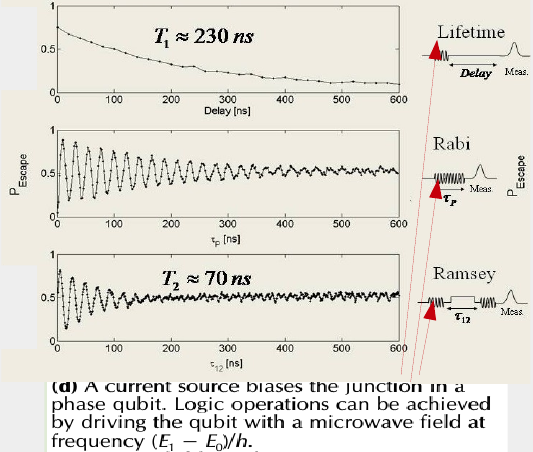
\includegraphics[width=0.5\textwidth]{immagini/phase_qubits_oscillations.png}
\end{figure}
\hspace{-0.6cm}Consideriamo ad esempio le oscillazioni di Rabi, cioè oscillazioni che vengono indotte quando abbiamo un sistema a due livelli pilotato con un drive periodico risonante con la transizione, che è precisamente ciò che facciamo quando applichiamo un drive con frequenza $\omega_{01}$.\\
Quello che osserviamo in queste misure è qualcosa che non ci aspetteremmo. Infatti questo grafico deriva dalla misura degli impulsi di corrente. Misurare questi impulsi equivale in realtà a misurare la probabilità che il sistema si trovi nello stato $\ket*{1}$, che idealmente dovrebbe comportarsi come $\cos^2{(\omega_{01} t)}$. Il punto è che la descrizione basata soltanto sull'hamiltoniana del dispositivo corrisponde a un sistema isolato. In pratica però non abbiamo incluso l'interazione con il resto del circuito. Ad esempio, la cosa più semplice che non abbiamo incluso è la resistenza presente nel circuito.\\
Ma questo non è l'unico effetto: in generale esiste un'interazione del sistema con l'ambiente esterno, che induce un decadimento delle oscillazioni, nel caso più semplice perché abbiamo dissipazione, cioè perdita di energia, quando il sistema è accoppiato all'ambiente.\\
In molti casi questo effetto viene descritto assumendo che la probabilità di trovare il sistema nello stato $\ket*{1}$ abbia la forma
\begin{equation*}
    \mathbb{P}_{\ket*{1}}(t)
    =\cos^2{(\omega_{01} t)} e^{-t/\tau_1}
\end{equation*}
Molto spesso quindi compare un decadimento esponenziale con una scala temporale $\tau_1$, chiamata tempo di rilassamento, che descrive nel caso più semplice le perdite di energia dovute all'interazione con l'ambiente esterno e in particolare con le sorgenti dissipative.\\
Un altro effetto che può comparire è chiamato \emph{leakage}. Il leakage è una proprietà tipica di un sistema multi-livello. In pratica il sistema possiede un certo numero di livelli energetici e noi abbiamo deciso di concentrarci sui due livelli più bassi, il che è ragionevole, ma resta comunque possibile che il sistema esca da questo sottospazio ridotto.\\
Questo decadimento viene generalmente chiamato \emph{decoerenza}, cioè decadimento delle oscillazioni coerenti. In pratica questo rappresenta uno dei principali problemi delle implementazioni a stato solido dei qubit.\\
Quello che abbiamo discusso finora riguarda il phase qubit. In realtà esiste una vera e propria ``giungla'' di qubit basati su giunzioni Josephson:
\begin{figure}[H]
    \centering
    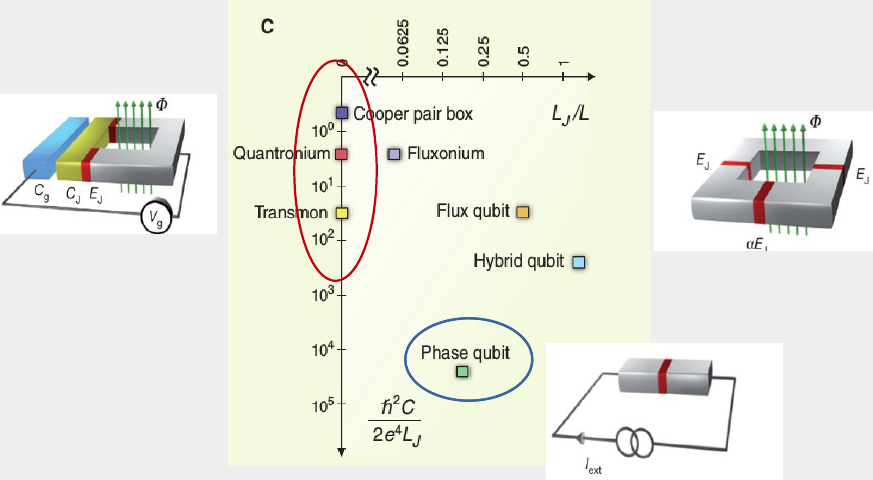
\includegraphics[width=0.8\textwidth]{immagini/jungle_qubits.png}
\end{figure}
\hspace{-0.6cm}La differenza principale tra questi dispositivi è la dimensione delle giunzioni, cioè giunzioni più grandi o più piccole, il che implica avere energie Josephson differenti e anche configurazioni circuitali differenti.\\
Oltre al dispositivo visto finora, esistono infatti architetture molto diverse. Discuteremo ad esempio del Cooper pair box, del Quantronium e del Transmon, che appartengono tutti alla famiglia dei cosiddetti qubit basati sulla carica. L'altra grande famiglia è quella dei qubit basati sul flusso.\\
La distinzione tra queste due famiglie si vede nel diagramma, dove i due parametri sugli assi sono:
\begin{itemize}[leftmargin=0.5cm]
    \item l'induttanza sull'asse $y$;
    \item una combinazione di parametri che scala con la capacità sull'asse $x$.
\end{itemize}
Le configurazioni sono schematizzate nella figura. I qubit basati sul grado di libertà di carica (e vedremo tra poco cosa significa precisamente) hanno una struttura come quella a sinistra, dove la parte gialla è un elettrodo superconduttivo e le due parti rosse sono due giunzioni Josephson. Esse sono collegate a un altro elettrodo, rappresentato in grigio, anch'esso superconduttivo.\\
Il punto importante è che l'elettrodo giallo, che è più piccolo degli altri, si trova di fronte a un altro elettrodo, anch'esso tipicamente superconduttivo. Con questa geometria possiamo considerare la carica accumulata sulla cosiddetta \emph{superconducting island} come una quantità rilevante nel comportamento del dispositivo, e vedremo più avanti in maniera più precisa cosa questo significhi.\\
I qubit basati sulla carica sono quindi dispositivi in cui esiste un elettrodo superconduttivo sul quale possiamo considerare rilevante la carica accumulata. Naturalmente si tratta di carica di coppie di Cooper.\\
L'altra configurazione, chiamata \emph{flux based qubits}, è invece tipicamente basata su un anello superconduttivo interrotto da alcune giunzioni Josephson, generalmente più di una, come si vede nella figura a destra.\\
In questo caso non esiste un'isola speciale: le tre parti del circuito sono più o meno equivalenti e non abbiamo un altro elettrodo posto di fronte all'isola, perché nei dispositivi della famiglia precedente il punto chiave era proprio la presenza di un accoppiamento capacitivo elettrostatico con un elettrodo esterno, cosa che qui non avviene.\\
Di conseguenza, in questo caso il grado di libertà rilevante per codificare l'informazione è l'operatore di flusso.\\
Quindi, a seconda delle dimensioni delle giunzioni e della configurazione circuitale in cui le giunzioni sono inserite, possiamo ottenere dispositivi in cui la variabile quantistica più rilevante è la carica elettrostatica oppure il flusso magnetico.\\
Ricordiamo infine che carica e flusso sono variabili coniugate, quindi le diverse configurazioni circuitali determinano quale delle due variabili diventa dominante nella dinamica del dispositivo.
\section{Cooper pair box}
Descriviamo ora i blocchi fondamentali di questo tipo di circuito. Partiamo dal qubit di carica. Il circuito più semplice è il cosiddetto \emph{Cooper pair box}, cioè una ``scatola'' per coppie di Cooper, schematizzata nel modo seguente:
\begin{figure}[H]
    \centering
    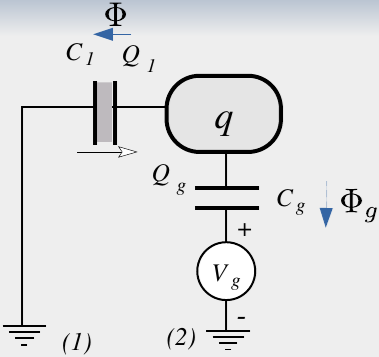
\includegraphics[width=0.45\textwidth]{immagini/Cooper_pair_box.png}
\end{figure}
\hspace{-0.6cm}Abbiamo un'isola superconduttiva, rappresentata come una scatola, che costituisce un elettrodo superconduttivo. Questo elettrodo è isolato dal resto del circuito tramite una giunzione Josephson; quindi ciò che abbiamo schematizzato come la capacità $C_1$ è in realtà una giunzione Josephson.\\
Questa è quindi una descrizione elettrostatica della giunzione e dell'elettrodo, nella quale vogliamo enfatizzare il fatto che la giunzione possiede anche una capacità.\\
Di fronte a questo elettrodo ne abbiamo un altro, con il quale esiste un accoppiamento elettrostatico descritto dalla capacità $C_g$, dove il pedice $g$ sta per ``gate'', perché questo elettrodo è collegato a una sorgente di tensione, la tensione di gate $V_g$.\\
\subsection{L'hamiltoniana}
Quello che dobbiamo fare ora è scrivere la descrizione elettrostatica del circuito considerando la parte elettrostatica e l'energia Josephson. Per la parte elettrostatica dobbiamo semplicemente descrivere il circuito come in elettromagnetismo classico, considerando l'energia elettrostatica associata alla presenza di una certa carica $Q$ sull'isola.\\
Poiché l'isola è accoppiata elettrostaticamente alla tensione di gate, la carica efficace sarà $Q + C_g V_g$, mentre la capacità totale sarà $C_\Sigma$, data dalla somma della capacità della giunzione Josephson e di $C_g$.\\
In aggiunta dobbiamo includere la possibilità di avere energia Josephson. L'hamiltoniana complessiva sarà quindi
\begin{equation*}
    \mathcal{H}=\frac{(Q + C_g V_g)^2}{2 C_{\Sigma}} - E_J \cos{ \qty( \frac{2 \pi \Phi}{\Phi_0} ) }
\end{equation*}
dove abbiamo espresso la differenza di fase in termini del flusso magnetico.\\
Il termine Josephson è quindi il solito termine $- E_J \cos(\varphi)$, e ancora una volta colleghiamo la differenza di fase al flusso magnetico. Anche se qui il circuito non è rappresentato esplicitamente come un anello, bisogna capire che anche in questa configurazione l'energia Josephson può essere espressa in termini del flusso.\\
Questa Hamiltoniana deriva quindi da una descrizione classica del sistema, nel senso che assumiamo che l'elemento Josephson abbia un'energia data da questa espressione.\\
Qual è il passo successivo? Dal momento che siamo partiti scrivendo l'hamiltoniana, dobbiamo verificare che da essa si ottengano correttamente le equazioni del moto delle diverse variabili. A partire dalle equazioni del moto possiamo poi controllare che vengano riprodotte le corrette equazioni circuitali del dispositivo.\\
C'è però un punto importante da considerare. Abbiamo detto che, per una giunzione Josephson isolata, carica e fase sono variabili coniugate. Quando però la giunzione è inserita in un circuito, bisogna identificare correttamente quali siano le variabili coniugate appropriate.\\
Quello che dobbiamo fare è quindi considerare il flusso magnetico come coordinata generalizzata e identificare il momento coniugato. Il punto fondamentale è che il corretto operatore di carica non è necessariamente semplicemente $Q$: bisogna prestare attenzione alla struttura del circuito.\\
In questo caso, diversamente dal phase qubit, la quantità rilevante non è la carica sulla giunzione, ma la carica totale presente sull'isola superconduttiva.\\
Il punto chiave è che la giunzione Josephson e la capacità di gate sono descritte da coordinate generalizzate differenti: $\Phi$ e $\Phi_g$. Dobbiamo quindi prestare molta attenzione alla struttura del circuito.\\
Queste due variabili sono legate dal vincolo imposto dalle cadute di tensione:
\begin{equation*}
    \dot{\Phi} + \dot{\Phi}_g = V_g
\end{equation*}
Il modo corretto di procedere per identificare la variabile coniugata è esattamente lo stesso che si utilizza nella descrizione classica dei sistemi meccanici:
\begin{itemize}[leftmargin=0.5cm]
    \item si parte dalla lagrangiana;
    \item si identificano le variabili coniugate;
    \item si passa all'hamiltoniana;
    \item infine si quantizza il sistema.
\end{itemize}
In altre parole, siamo partiti dall'Hamiltoniana del dispositivo. Quello che dobbiamo fare è verificare che le equazioni di Hamilton riproducano correttamente le equazioni circuitali.\\
Per mostrarlo, procediamo nel verso opposto:
\begin{itemize}[leftmargin=0.5cm]
    \item partiamo dalle equazioni del circuito;
    \item imponiamo i vincoli tra le variabili;
    \item scriviamo il termine cinetico;
    \item identifichiamo la carica tramite le equazioni di Lagrange;
    \item costruiamo l'Hamiltoniana includendo sia il contributo cinetico sia l'energia Josephson.
\end{itemize}
In questo modo ritroveremo l'Hamiltoniana da cui siamo partiti inizialmente.\\
Facciamolo esplicitamente. Partiamo dalla parte cinetica:
\begin{equation*}
    K
    =
    \frac{C}{2} \dot{\Phi}^2 + \frac{C_g}{2} \dot{\Phi}_g^2
    =
    \frac{C}{2} \dot{\Phi}^2 + \frac{C_g}{2} (V_g - \dot{\Phi})^2
\end{equation*}
dove nel secondo passaggio abbiamo utilizzato il vincolo precedente.\\
Ora possiamo identificare la variabile coniugata:
\begin{equation*}
    Q
    =\frac{\partial K}{\partial \dot{\Phi}}
    =C \dot{\Phi} - C_g (V_g - \dot{\Phi})
\end{equation*}
da cui otteniamo
\begin{equation*}
    Q=(C + C_g)\dot{\Phi} -C_g V_g
\end{equation*}
e quindi
\begin{equation*}
    \dot{\Phi}
    =\frac{Q + C_g V_g}{C + C_g}
    =\frac{Q + C_g V_g}{C_{\Sigma}}
\end{equation*}
L'Hamiltoniana sarà data da
\begin{equation*}
    \mathcal{H}
    =Q \dot{\Phi} - K + U(\Phi)
\end{equation*}
Per ottenere la forma finale dell'Hamiltoniana, esplicitiamo il quadrato presente in $K$:
\begin{equation*}
    K
    =\frac{C}{2} \dot{\Phi}^2 + \frac{C_g}{2} (V_g^2 - 2 V_g \dot{\Phi} + \dot{\Phi}^2)
    =\frac{C_{\Sigma}}{2} \dot{\Phi}^2 - C_g V_g \dot{\Phi} + \frac{C_g}{2} V_g^2
\end{equation*}
L'Hamiltoniana è quindi
\begin{equation*}
    \begin{split}
        \mathcal{H}
        & =C_{\Sigma}\dot{\Phi}^2 - C_g V_g \dot{\Phi} - \frac{C_{\Sigma}}{2} \dot{\Phi}^2 + C_g V_g \dot{\Phi} - \frac{C_g}{2} V_g^2 + U(\Phi)
        \\
        & =\frac{C_{\Sigma}}{2} \dot{\Phi}^2 - \frac{C_g}{2} V_g^2 + U(\Phi)
    \end{split}
\end{equation*}
Esprimiamo infine $\dot{\Phi}$ in termini di $Q$:
\begin{equation*}
    \mathcal{H}
    =\frac{(Q + C_g V_g)^2}{2 C_{\Sigma}} - \frac{C_g}{2} V_g^2 + U(\Phi)
\end{equation*}
Il termine $-\frac{C_g}{2} V_g^2$ è una costante che non dipende dalle variabili dinamiche del sistema, quindi possiamo semplicemente assorbirlo in una ridefinizione dell'energia di riferimento. In questo modo otteniamo l'Hamiltoniana finale:
\begin{equation*}
    \mathcal{H}
    =\frac{(Q + C_g V_g)^2}{2 C_{\Sigma}} - E_J \cos{ \qty( \frac{2 \pi \Phi}{\Phi_0} )}
\end{equation*}
\subsection{Quantizzazione e spettro}
In questo modo otteniamo un'Hamiltoniana classica, ma scritta in una forma tale da poter essere immediatamente quantizzata imponendo relazioni di commutazione tra le variabili coniugate. Assumiamo quindi di poter trattare queste quantità come variabili quantistiche e imponiamo la relazione di commutazione canonica. In questo modo otteniamo l'Hamiltoniana quantistica:
\begin{equation}
    \hat{\mathcal{H}}
    =
    E_C \bigl( \hat{q} + q_g \bigr)^2
    -
    E_J \cos{\hat{\phi}}
    \label{eq:hamiltonian_cooper_pair_box}
\end{equation}
dove
\begin{equation*}
    E_C
    =
    \frac{(2e)^2}{2(C + C_g)}
\end{equation*}
è l'energia elettrostatica associata alla presenza di una coppia di Cooper, mentre
\[
q=\frac{Q}{2e}
\qquad\text{e}\qquad
\phi=\frac{2e\Phi}{\hbar}
\]
sono le variabili adimensionali di carica e flusso. Abbiamo inoltre definito
\[
q_g=\frac{C_g V_g}{2e},
\]
che rappresenta la carica di gate adimensionale.\\
Nel procedere con questa quantizzazione dobbiamo tenere presente che, diversamente dal caso di una particella classica descritta da una variabile continua, dove $x$ e $p$ sono variabili coniugate ma $x$ può assumere qualsiasi valore, qui abbiamo quantità discrete. In particolare, la carica è discreta, perché descrive un numero intero addizionale di coppie di Cooper.\\
Dobbiamo tenere conto di questo fatto quando consideriamo le proprietà delle corrispondenti funzioni d'onda. In altre parole, $\hat{q}$ è un operatore che descrive la carica sull'isola, quindi ci aspettiamo che abbia uno spettro discreto, cioè autovalori
\[
q=0,1,2,\ldots
\]
Se $\hat{q}$ ha uno spettro discreto, allora la funzione d'onda deve essere periodica. Questo è esattamente ciò che accade, ad esempio, per una particella classica soggetta a condizioni periodiche al contorno.\\
Lo si vede facilmente osservando che le relazioni di commutazione imposte implicano che $\hat{q}$ sia rappresentato da $-i\partial_\phi$. Questo è naturale, perché la carica è il momento coniugato del flusso, proprio come $p$ è il momento coniugato di $x$, e possiede quindi una rappresentazione analoga.\\
Agendo quindi sulla funzione d'onda corrispondente all'autovalore $q$, abbiamo
\begin{equation*}
    \hat{q} \ket*{q}
    =
    q \ket*{q}
    \implies
    -i \partial_{\phi}\chi_q(\phi)
    =
    q \chi_q(\phi)
\end{equation*}
dove $\chi_q$ è l'autofunzione associata all'autovalore $q$.\\
Questa equazione è semplicemente risolta dalla funzione d'onda
\begin{equation*}
    \chi_q(\phi)
    =
    A e^{iq\phi}.
\end{equation*}
Gli autovalori risultano discreti se e solo se le funzioni d'onda sono periodiche, cioè se
\[
\psi(\phi)=\psi(\phi+2\pi)
\]
Questo fornisce quindi un modo semplice per vedere che la discrezione degli autovalori della carica corrisponde a funzioni d'onda periodiche nella coordinata flusso.\\
Quello che vogliamo ora analizzare è lo spettro, cioè i livelli energetici di questa Hamiltoniana corrispondenti agli autovalori discreti della carica.\\
Per farlo consideriamo l'\eqrefcustom{eq:hamiltonian_cooper_pair_box} e supponiamo inizialmente di non avere il termine Josephson. In queste condizioni l'Hamiltoniana diventa
\begin{equation*}
    \hat{\mathcal{H}}
    =
    E_C \bigl( \hat{q}+q_g \bigr)^2
\end{equation*}
Gli autostati saranno chiaramente autostati dell'operatore carica, perché non compare alcun'altra variabile quantistica. Infatti, in questo caso, l'Hamiltoniana commuta con l'operatore carica:
\[
\bigl[\hat{\mathcal{H}},\hat{q}\bigr]=0,
\]
quindi possiamo trovare autostati comuni:
\begin{equation*}
    \hat{\mathcal{H}}\ket*{\psi_q}
    =
    E_C \bigl(q+q_g\bigr)^2 \ket*{\psi_q}.
\end{equation*}
Gli autolivelli sono quindi
\begin{equation*}
    E_q(q_g)
    =
    E_C \bigl(q+q_g\bigr)^2
    \qq{,}
    q=0,1,2,\ldots
\end{equation*}
Possiamo rappresentare questi autovalori in funzione di $q_g$, quantità che possiamo controllare variando la tensione di gate:
\begin{figure}[H]
    \centering
    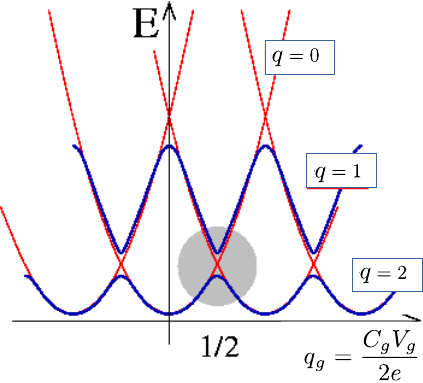
\includegraphics[width=0.5\textwidth]{immagini/parabolas_eigenlevels_CPB.png}
\end{figure}
\hspace{-0.6cm}Ad esempio:
\[
E_0(q_g)=E_C q_g^2,
\]
mentre per $q=1$ abbiamo
\[
E_1(q_g)=E_C(1+q_g)^2,
\]
e così via.\\
Vediamo quindi una serie di parabole, ciascuna associata a un diverso valore di $q$ e con minimo in $q_g=-q$.\\
L'idea è che, fissando nel circuito un determinato valore $\bar{q}_g$, otteniamo un dispositivo fisso i cui autolivelli possono essere letti semplicemente tracciando una linea verticale nel diagramma:
\begin{figure}[H]
    \centering
    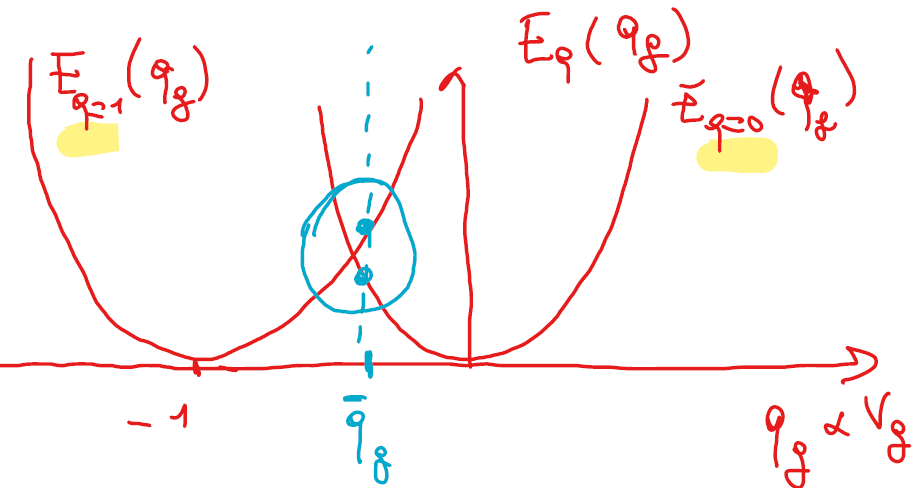
\includegraphics[width=0.5\textwidth]{immagini/parabolas_eigenlevels_CPB_fixed_qg.png}
\end{figure}
\hspace{-0.6cm}Come si vede dalla figura, gli autolivelli superiori sono molto più alti in energia rispetto ai due più bassi. Questo significa che, fissata una tensione di gate, possiamo identificare un sottospazio bidimensionale di autostati completamente isolato energeticamente dagli altri livelli.\\
Questi due livelli energetici più bassi, insieme ai corrispondenti autostati, costituiranno il nostro sottospazio computazionale bidimensionale, cioè gli stati $\ket*{0}$ e $\ket*{1}$ che vogliamo manipolare.\\
Finora abbiamo considerato soltanto la parte elettrostatica, trascurando completamente il termine Josephson. Vogliamo ora capire quale sia l'effetto dell'energia Josephson su questo diagramma.\\
Se operiamo nel cosiddetto \emph{charge regime}, l'energia Josephson è molto più piccola dell'energia di carica. Questo significa che possiamo trattare il termine Josephson come una perturbazione rispetto alla parte elettrostatica.\\
In linea di principio potremmo quindi scrivere le correzioni perturbative agli autolivelli e agli autostati. Tuttavia sappiamo che, dal punto di vista quantistico, la prima cosa che una perturbazione fa in presenza di degenerazioni è rimuoverle.\\
Questo significa che il potenziale viene modificato come mostrato nella figura precedente dalle curve blu, che rappresentano gli autovalori corretti includendo il termine Josephson.\\
Se osserviamo la zona di intersezione tra le parabole, vediamo infatti che la degenerazione scompare: i livelli non si incrociano più, ma vengono separati da un'energia che è proprio dell'ordine dell'energia Josephson.\\
Naturalmente i livelli vengono modificati anche nelle altre regioni, ma lì la correzione è perturbativa. Infatti le curve rosse e blu non coincidono esattamente, ma risultano solo leggermente separate a causa della correzione energetica introdotta dalla perturbazione.\\
Il messaggio principale è quindi che, quando consideriamo sia la parte elettrostatica sia l'energia Josephson, possiamo ancora ottenere — per opportuni valori della tensione di gate, cioè vicino ai punti di quasi-degenerazione — un sistema efficace a due livelli, perché tutti gli altri livelli rimangono molto più alti in energia.\\
Tuttavia, i due livelli non sono più degeneri. Nel caso precedente non ci eravamo posizionati esattamente nel punto di degenerazione, ma leggermente spostati; se ci fossimo messi esattamente nel punto di incrocio avremmo avuto una vera degenerazione.\\
Anche includendo l'energia Josephson, se fissiamo il potenziale vicino a uno di questi punti di quasi-degenerazione, possiamo ancora ottenere un sistema efficace a due livelli sufficientemente isolato dagli altri.\\
Gli autostati, però, non saranno più puri stati di carica: diventeranno sovrapposizioni di stati di carica.
\subsection{Relazioni tra operatori e rappresentazione in carica}
Introduciamo ora la rappresentazione in carica del Cooper Pair Box.\\
Le variabili quantistiche rilevanti sono la differenza di fase superconduttiva $\hat{\phi}$ attraverso la giunzione Josephson e l'operatore $\hat{q}$, che rappresenta il numero di coppie di Cooper presenti sull'isola superconduttiva.\\
Queste due quantità sono variabili canonicamente coniugate e soddisfano la relazione di commutazione
\[
[\hat{q},\hat{\phi}]=i.
\]
Tuttavia, diversamente dal consueto operatore posizione in meccanica quantistica, la fase è una variabile periodica:
\[
\phi \equiv \phi + 2\pi
\]
Per questa ragione, gli operatori fisicamente significativi non sono $\hat{\phi}$ stesso, ma piuttosto funzioni periodiche della fase, come $e^{\pm i\hat{\phi}}$ oppure $\cos\hat{\phi}$.\\
La corretta relazione di commutazione si scrive quindi nella forma
\begin{equation*}
    [\hat{q},e^{\pm i\hat{\phi}}]=\pm e^{\pm i\hat{\phi}}
\end{equation*}
Gli operatori $e^{\pm i\hat{\phi}}$ agiscono come operatori di traslazione nella base di carica. Se $\ket*{q}$ denota uno stato con $q$ coppie di Cooper sull'isola, allora
\begin{equation*}
    e^{\pm i\hat{\phi}} \ket*{q}=\ket*{q \pm 1}
\end{equation*}
L'operatore $e^{+i\hat{\phi}}$ aggiunge quindi una coppia di Cooper all'isola, mentre $e^{-i\hat{\phi}}$ rimuove una coppia di Cooper.\\
Nella base di carica questi operatori possono essere scritti come
\begin{equation*}
    e^{\pm i\hat{\phi}}=\sum_q \ketbra*{q \pm 1}{q}
\end{equation*}
Utilizzando l'identità
\begin{equation*}
    \cos\hat{\phi}
    =
    \frac{1}{2}
    \qty(
        e^{i\hat{\phi}}
        +
        e^{-i\hat{\phi}}
    )
\end{equation*}
otteniamo
\begin{equation*}
    \cos\hat{\phi}
    =
    \frac{1}{2}
    \sum_q
    \ketbra*{q+1}{q}
    +
    \text{h.c.}
\end{equation*}
dove h.c. denota l'hermitiano coniugato.\\
L'Hamiltoniana del Cooper Pair Box può quindi essere scritta nella rappresentazione in carica come
\begin{equation*}
    \hat{\mathcal{H}}
    =
    E_C
    \sum_q
    \bigl(
        q + q_g
    \bigr)^2
    \ketbra*{q}{q}
    -
    \frac{E_J}{2}
    \sum_q
    \bigl(
        \ketbra*{q+1}{q}
        +
        \ketbra*{q}{q+1}
    \bigr).
\end{equation*}
Il primo termine rappresenta l'energia elettrostatica ed è diagonale nella base di carica. Il secondo termine deriva invece dall'accoppiamento Josephson e mescola stati di carica che differiscono di una coppia di Cooper.\\
In altre parole, l'effetto del termine Josephson è quello di indurre transizioni tra gli stati di carica. In particolare, induce transizioni tra gli stati energetici di carica più vicini, che differiscono precisamente per una coppia di Cooper. Per questo motivo, nella rappresentazione in carica esso è un operatore non diagonale: la sua azione consiste nel trasformare lo stato $\ket*{q}$ nello stato $\ket*{q \pm 1}$.\\
Questo è sostanzialmente lo stesso effetto che un operatore quantità di moto produce agendo sugli autostati della posizione. L'operatore quantità di moto, infatti, agisce come generatore di traslazioni. Quindi, se consideriamo autostati della posizione descritti da onde piane e agiamo su di essi con l'operatore quantità di moto, ciò che otteniamo è una traslazione del momento di una certa quantità.
\subsection{Dal Cooper pair box al charge qubit}
Se scegliamo $q_g$ vicino a uno degli stati di energia più bassa, possiamo ridurre lo spazio di Hilbert ai soli stati a energia minima. Matematicamente questo significa proiettare l'Hamiltoniana completa nel sottospazio generato da questi due autostati. Tale proiezione si realizza tramite l'operatore
\begin{equation*}
    \hat{P}
    =
    \ketbra*{0}{0}
    +
    \ketbra*{1}{1}
\end{equation*}
Il risultato è un'Hamiltoniana $2 \times 2$:
\begin{equation*}
    \hat{P}\hat{\mathcal{H}}_{\text{CPB}}\hat{P}
    =
    E_C
    \bigl[
        q_g^2 \ketbra*{0}{0}
        +
        (1+q_g)^2 \ketbra*{1}{1}
    \bigr]
    -
    \frac{E_J}{2}
    \bigl(
        \ketbra*{1}{0}
        +
        \ketbra*{0}{1}
    \bigr).
\end{equation*}
Questa Hamiltoniana consiste di due parti:
\begin{itemize}[leftmargin=0.5cm]
    \item la parte elettrostatica, che possiede due autovalori dipendenti da $q_g$;
    \item la parte Josephson, che agisce nella base di carica come un operatore che scambia gli stati con zero e una coppia di Cooper.
\end{itemize}
Quest'ultimo punto è naturale, perché sappiamo già che l'effetto Josephson corrisponde a una supercorrente che attraversa la giunzione. Se da un lato della giunzione è presente un'isola superconduttiva, allora la supercorrente modifica il numero di coppie di Cooper presenti sull'isola.\\
Poiché stiamo lavorando in un sottospazio $2 \times 2$, possiamo rappresentare l'Hamiltoniana utilizzando le matrici di Pauli.\\
La parte elettrostatica, essendo diagonale nella base di carica, può essere rappresentata tramite $\sigma_z$, mentre la parte Josephson, che è non diagonale nella base di carica, può essere rappresentata tramite $\sigma_x$. In particolare, la parte elettrostatica assume la forma
\begin{equation*}
    E_C
    \begin{pmatrix}
        q_g^2 & 0 \\
        0 & (1+q_g)^2
    \end{pmatrix}
\end{equation*}
Questa matrice può essere riscritta come somma di un termine proporzionale all'identità e di un termine proporzionale a $\sigma_z$:\sn{In generale, una matrice del tipo
\begin{equation*}
    \begin{pmatrix}
        a & 0 \\
        0 & b
    \end{pmatrix}
\end{equation*}
può essere scritta come
\begin{equation*}
    \frac{a+b}{2}\1 + \frac{a-b}{2}\sigma_z
\end{equation*}
dove $\1$ è la matrice identità. Nel nostro caso $a=q_g^2$ e $b=(1+q_g)^2$.}
\begin{equation*}
    E_C
    \begin{pmatrix}
        q_g^2 & 0 \\
        0 & (1+q_g)^2
    \end{pmatrix}
    =
    \frac{E_C}{2}
    \bigl(
        2q_g^2 + 2q_g + 1
    \bigr)\1
    -
    \frac{\epsilon}{2}\sigma_z
\end{equation*}
dove
\begin{equation*}
    \epsilon \equiv \epsilon(q_g)
    =
    E_C(1+2q_g)
\end{equation*}
rappresenta lo splitting energetico tra i due stati di carica.\\
Il termine Josephson in questa rappresentazione è invece dato da
\begin{equation*}
    -\frac{E_J}{2}
    \begin{pmatrix}
        0 & 1 \\
        1 & 0
    \end{pmatrix}
    =
    -\frac{\Delta}{2}\sigma_x
\end{equation*}
dove
\[
\Delta = E_J.
\]
Quindi la proiezione dell'Hamiltoniana del Cooper pair box nel sottospazio degli stati a più bassa energia può essere espressa semplicemente tramite le matrici di Pauli $\sigma_z$ e $\sigma_x$:
\begin{equation*}
    \hat{P}\hat{\mathcal{H}}_{\text{CPB}}\hat{P}
    =
    \frac{E_C}{2}
    \bigl(
        2q_g^2 + 2q_g + 1
    \bigr)\1
    -
    \frac{\epsilon}{2}\sigma_z
    -
    \frac{\Delta}{2}\sigma_x.
\end{equation*}
Spesso il termine proporzionale all'identità viene omesso, perché rappresenta soltanto uno shift energetico globale che non modifica la dinamica del sistema. In tal caso si ottiene l'Hamiltoniana efficace del charge qubit:
\begin{equation*}
    \hat{\mathcal{H}}_{\rm qubit}
    =
    - \frac{\epsilon}{2}\sigma_z
    - \frac{\Delta}{2}\sigma_x
\end{equation*}
dove:
\begin{itemize}[leftmargin=0.5cm]
    \item $\sigma_z$ deriva dalla parte elettrostatica, cioè dall'operatore di carica;
    \item $\sigma_x$ deriva invece dal termine Josephson, cioè dall'operatore di fase.
\end{itemize}
\subsection{Charge qubit pilotato tramite impulsi rapidi}
A questo punto abbiamo fatto qualcosa di molto simile a quanto avevamo fatto per il phase qubit: siamo partiti dalla descrizione circuitale del Cooper pair box, abbiamo identificato autolivelli e autostati e visto che possiamo isolare una coppia di stati a bassa energia che rappresenta il nostro sottospazio computazionale. In definitiva, possiamo trattare il sistema come un sistema efficace a due livelli, cioè il nostro qubit.\\
Il passo successivo consiste nel fare esattamente ciò che abbiamo fatto per il phase qubit: preparare il sistema in un certo stato, lasciarlo evolvere e infine misurarlo. L'evoluzione può essere:
\begin{itemize}[leftmargin=0.5cm]
    \item evoluzione libera, quindi oscillazioni di Maiorana;
    \item oppure un'evoluzione guidata, se vogliamo effettuare operazioni sul qubit, ad esempio oscillazioni di Rabi.
\end{itemize}
In questo caso l'unico parametro di controllo disponibile è la tensione di gate. Possiamo quindi aggiungere alla tensione di gate una componente oscillante nel tempo e ottenere oscillazioni di Rabi nel sistema efficace a due livelli che abbiamo identificato.\\
In generale possiamo considerare una tensione di gate dipendente dal tempo:
\[
q_g \to q_g + \delta q_g(t).
\]
Questo significa aggiungere all'Hamiltoniana una parte di controllo $\hat{\mathcal{H}}_{\text{c}}(t)$, che assume la forma semplice
\begin{equation*}
    \hat{\mathcal{H}}_{\text{c}}(t)
    =
    -E_C \delta q_g(t)\sigma_z
\end{equation*}
poiché $\sigma_z$ è la matrice di Pauli associata all'operatore di carica.\\
L'Hamiltoniana totale di controllo diventa quindi
\begin{equation*}
    \hat{\mathcal{H}}(t)
    =
    -\frac{1}{2}
    \bigl[
        \epsilon + \delta\epsilon(t)
    \bigr]
    \sigma_z
    -
    \frac{E_J(\Phi_x)}{2}\sigma_x
\end{equation*}
dove, invece del solo $\epsilon$, compare
\[
\epsilon + \delta\epsilon(t),
\]
con
\[
\delta\epsilon(t)=2E_C\delta q_g(t),
\]
quantità legata alla tensione di controllo.\\
Con la tensione di gate possiamo fare diverse cose:
\begin{itemize}[leftmargin=0.5cm]
    \item pilotare periodicamente il sistema;
    \item oppure applicare impulsi DC.
\end{itemize}
Nel secondo caso possiamo avere una tensione di gate $V_g(t)$ che non varia periodicamente, ma assume una forma a gradino: ad esempio il gate può essere inizialmente spento, poi acceso per un certo intervallo temporale e infine nuovamente spento.
\begin{figure}[H]
    \centering
    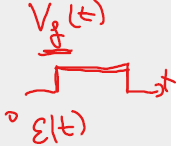
\includegraphics[width=0.3\textwidth]{immagini/pulse_gate_voltage.png}
\end{figure}
\hspace{-0.6cm}Vogliamo fare questo perché modificando la tensione di gate modifichiamo di fatto $\epsilon$, cioè uno dei contributi dell'Hamiltoniana a due livelli, che diventa quindi dipendente dal tempo. In pratica, cambiando $\epsilon$, modifichiamo il peso relativo dei diversi contributi dell'Hamiltoniana.\\
Vediamo questo punto più precisamente. Possiamo rappresentare questa Hamiltoniana tramite la sfera di Bloch, che costituisce una rappresentazione molto conveniente per un sistema a due livelli.\\
In questa rappresentazione abbiamo:
\begin{itemize}[leftmargin=0.5cm]
    \item un asse $z$, associato all'operatore di carica;
    \item un asse $x$, associato all'operatore di fase.
\end{itemize}
Possiamo quindi rappresentare l'Hamiltoniana come un vettore nel piano definito da questi due assi. La componente lungo $z$ è data da $\epsilon$, mentre quella lungo $x$ è data da $\Delta$.\\
Questa rappresentazione è particolarmente utile perché permette di visualizzare immediatamente il peso relativo dei diversi termini dell'Hamiltoniana e l'effetto della variazione dei suoi parametri.\\
Ad esempio:
\begin{itemize}[leftmargin=0.5cm]
    \item se scegliamo una tensione di gate tale da annullare il contributo elettrostatico, l'Hamiltoniana punterà lungo la direzione $x$;
    \item se invece $\epsilon \gg E_J$, l'Hamiltoniana sarà quasi interamente orientata lungo $z$.
\end{itemize}
Possiamo quindi visualizzare l'Hamiltoniana come un vettore sulla sfera di Bloch, la cui direzione dipende dai parametri del circuito.\\
Questa possibilità viene utilizzata per manipolare il charge qubit tramite impulsi rapidi, cioè variazioni improvvise della tensione di gate. Tali impulsi possono essere realizzati con grande accuratezza, su scale temporali dell'ordine delle frazioni di nanosecondo.\\
Vediamo ora come appare l'Hamiltoniana quando modifichiamo la tensione di gate.
\begin{figure}[H]
    \centering
    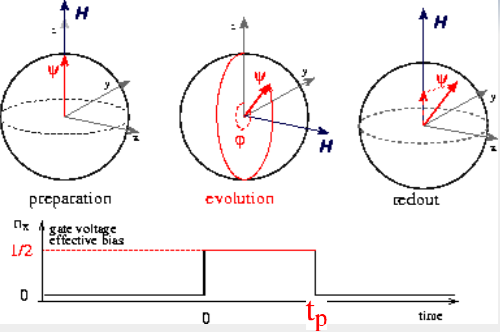
\includegraphics[width=0.6\textwidth]{immagini/bloch_sphere_hamiltonian.png}
\end{figure}
\hspace{-0.6cm}Sull'asse verticale compare $q_x$, legato alla tensione di gate. Partiamo da tensione di gate nulla, con
\[
E_C \gg E_J.
\]
Questo significa che, fintanto che la tensione di gate è nulla, l'Hamiltoniana possiede una componente dominante lungo la direzione $z$. In pratica, il vettore Hamiltoniano punta lungo $z$.\\
Se l'Hamiltoniana punta lungo $z$, i suoi autostati saranno gli autostati di $\sigma_z$. Operando a temperatura sufficientemente bassa, il sistema rilasserà verso lo stato fondamentale dell'Hamiltoniana.\\
Quindi, se manteniamo nulla la tensione di gate e aspettiamo un tempo sufficientemente lungo, il sistema si troverà sicuramente nello stato fondamentale associato alla direzione $z$, rappresentato sulla sfera di Bloch come uno stato allineato con l'Hamiltoniana.\\
Supponiamo ora di accendere molto rapidamente la tensione di gate, portando il sistema al valore
\[
q_x=\frac{1}{2},
\]
che è precisamente il punto in cui i due livelli energetici sono separati soltanto da $E_J$.\\
Matematicamente, per
\[
q_g=\frac{1}{2},
\]
il contributo elettrostatico si annulla e l'Hamiltoniana punta interamente lungo la direzione $\sigma_x$.\\
Poiché questa modifica dell'Hamiltoniana avviene quasi istantaneamente, il sistema non ha il tempo di adattarsi o rilassare verso il nuovo autostato.\\
All'istante iniziale abbiamo quindi:
\begin{itemize}[leftmargin=0.5cm]
    \item un'Hamiltoniana orientata lungo $\sigma_x$;
    \item uno stato iniziale che è invece un autostato di $\sigma_z$.
\end{itemize}
Ma un autostato di $\sigma_z$ è una sovrapposizione degli autostati di $\sigma_x$. Questo significa che il sistema inizierà a oscillare coerentemente tra i due autostati di $\sigma_x$.\\
Sulla sfera di Bloch ciò corrisponde a una precessione attorno alla direzione dell'Hamiltoniana.\\
Questa evoluzione continua fino a quando modifichiamo nuovamente l'Hamiltoniana. Possiamo ad esempio spegnere il gate a un certo istante $t_p$, riportando l'Hamiltoniana nella direzione $z$.\\
In quell'istante il sistema si troverà in una sovrapposizione degli autostati di $\sigma_z$:
\begin{equation*}
    \ket*{\psi(t_p)}
    =
    c_0 \ket*{0}
    +
    c_1 \ket*{1}.
\end{equation*}
Ricordiamo infatti che:
\begin{itemize}[leftmargin=0.5cm]
    \item inizialmente il sistema era preparato in uno stato di $\sigma_z$;
    \item successivamente ha oscillato coerentemente tra gli autostati di $\sigma_x$, cioè $\ket*{+}$ e $\ket*{-}$.
\end{itemize}
L'evoluzione temporale è quindi
\begin{equation*}
    \ket*{\psi(t)}
    =
    \frac{1}{\sqrt{2}}
    \qty(
        e^{iE_J t/2}\ket*{+}
        +
        e^{-iE_J t/2}\ket*{-}
    ).
\end{equation*}
Quando spegniamo l'impulso, otteniamo quindi una sovrapposizione degli stati $\ket*{0}$ e $\ket*{1}$.\\
La probabilità di trovare il sistema nello stato $\ket*{0}$ dipende dalla durata dell'impulso:
\begin{equation*}
    p_0
    =
    |c_0|^2
    =
    \bigl|
        \braket*{0}{\psi(t)}
    \bigr|^2
    =
    \sin^2{
        \qty(
            \frac{E_J t}{2}
        )
    }.
\end{equation*}
Vediamo quindi che la probabilità di trovare il sistema nello stato $\ket*{0}$ dipende:
\begin{itemize}[leftmargin=0.5cm]
    \item dalla durata dell'impulso;
    \item dalla frequenza di oscillazione fissata da $E_J$.
\end{itemize}
Questa è la probabilità di trovare il sistema con zero coppie di Cooper aggiuntive sull'isola. La probabilità di avere invece una coppia di Cooper extra sarà
\[
p_1=1-p_0.
\]
L'ultimo passaggio consiste nel capire come misurare questa probabilità.\\
L'idea è la seguente. Se il sistema possiede una coppia di Cooper aggiuntiva sull'isola, cioè due elettroni extra, esiste una certa probabilità che questa coppia si rompa in quasiparticelle con carica $e$.\\
Questo può avvenire se il circuito è opportunamente collegato a una parte addizionale dedicata alla misura. Quando la coppia di Cooper decade in quasiparticelle, compare una corrente microscopica nel dispositivo di misura.\\
La misura consiste quindi nel rilevare questa corrente associata alla rottura della coppia di Cooper in stati di quasiparticella. Naturalmente questo richiede un ulteriore elemento circuitale dedicato alla lettura dello stato del qubit.
\section{Transmon qubit}
Consideriamo ora il transmon. L'idea è quella di avere un'isola superconduttiva isolata dal resto del circuito tramite la giunzione Josephson e le capacità che la collegano al circuito stesso. Abbiamo già visto che questo dispositivo può avere diverse implementazioni, una delle quali è schematizzata nella figura seguente:
\begin{figure}[H]
    \centering
    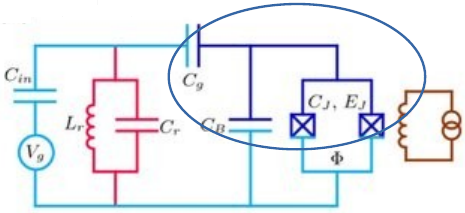
\includegraphics[width=0.6\textwidth]{immagini/transmon.png}
\end{figure}
\hspace{-0.6cm}In questo caso l'isola superconduttiva è la parte blu. Abbiamo quindi un loop superconduttivo interrotto da due giunzioni Josephson e una singola isola superconduttiva collegata al circuito tramite alcune capacità. L'ingrediente aggiuntivo fondamentale è però la capacità $C_B$, posta in parallelo alla giunzione complessiva.\\
Il ruolo di questa capacità addizionale è quello di capacità di shunt. Essa compare infatti nell'energia elettrostatica secondo
\begin{equation*}
    E_C
    =
    \frac{2e^2}{2C_J + C_g + C_S}
\end{equation*}
e, poiché è grande, rende molto più piccola l'energia di carica.\\
In questo modo otteniamo un circuito molto simile al Cooper pair box, ma con un diverso rapporto tra energia di carica ed energia Josephson. Abbiamo già visto che queste due energie giocano un ruolo fondamentale:
\begin{itemize}[leftmargin=0.5cm]
    \item l'energia di carica rende rilevanti gli effetti elettrostatici e quindi la variabile quantistica associata alla carica;
    \item l'energia Josephson rende invece rilevante la variabile quantistica associata alla fase o al flusso.
\end{itemize}
Se il dispositivo opera in questo regime, il primo effetto che osserviamo è una modifica della dipendenza degli autolivelli dalla tensione di gate, come mostrato nella figura seguente:
\begin{figure}[H]
    \centering
    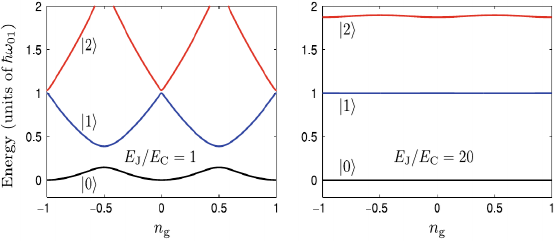
\includegraphics[width=0.7\textwidth]{immagini/transmon_eigenlevels.png}
\end{figure}
\hspace{-0.6cm}Nel grafico di sinistra vediamo gli autolivelli del Cooper pair box quando vengono considerati sia il contributo elettrostatico sia quello Josephson. Abbiamo già commentato che questi livelli dipendono dal parametro di controllo $n_g$, proporzionale alla tensione di gate, e che fissato il valore del gate gli autovalori del dispositivo si ottengono intersecando la verticale corrispondente con i livelli energetici.\\
Ciò che caratterizza il regime di carica, in particolare nel caso in cui $E_J$ ed $E_C$ siano confrontabili, è che i livelli energetici mostrano una forte dipendenza non monotona dalla tensione di gate.\\
Questo implica — e lo vedremo meglio più avanti — che tale implementazione è molto sensibile alle fluttuazioni della tensione di gate provenienti dal circuito elettrostatico. In pratica, anche se vorremmo mantenere il gate fissato a un certo valore, sono sempre presenti fluttuazioni dovute a diverse sorgenti fisiche.\\
Queste fluttuazioni fanno oscillare leggermente il cosiddetto operating point del dispositivo. Di conseguenza, ad esempio, anche lo splitting energetico tra i primi due livelli cambia nel tempo: se il bias fosse perfettamente fissato avremmo uno splitting ben definito, ma se la tensione di gate fluttua allora durante la misura il sistema presenterà valori leggermente diversi dello splitting tra i livelli. Questo costituisce un problema importante, che analizzeremo meglio in seguito.\\
Nel circuito transmon, dove il rapporto tra le due energie è diverso, la dipendenza degli autolivelli dalla tensione di gate diventa molto più debole, come mostrato nella figura di destra.\\
Da un lato questo è vantaggioso perché il sistema risulta meno sensibile alle fluttuazioni della tensione di gate; dall'altro però può creare problemi di addressability, poiché gli splitting energetici diventano sempre più vicini a quelli di un oscillatore armonico. In pratica, ripetendo lo stesso procedimento svolto in precedenza, si vede che gli splitting tra livelli adiacenti diventano molto simili tra loro.\\
Detto questo, poiché vogliamo una grande capacità di shunt per ridurre la sensibilità alle fluttuazioni del gate, cerchiamo di capire come emergano questi splitting energetici.\\
Per farlo procediamo come in precedenza, scrivendo l'Hamiltoniana del dispositivo. In questo caso, poiché l'energia dipende molto debolmente dalla tensione di gate, possiamo considerare un'Hamiltoniana in cui i termini principali sono:
\begin{itemize}[leftmargin=0.5cm]
    \item la parte elettrostatica con la capacità di shunt;
    \item il termine Josephson.
\end{itemize}
Trascuriamo quindi la dipendenza dal gate:
\begin{equation*}
    \hat{\mathcal{H}}
    =
    E_C \hat{Q}^2
    -
    E_J \cos{\hat{\phi}}
    =
    \frac{\hat{Q}^2}{2C+C_S}
    -
    E_J \cos{\hat{\phi}}
\end{equation*}
Per comprendere la struttura degli autovalori, osserviamo che il termine Josephson agisce come un potenziale periodico. Tuttavia, per studiare i livelli a bassa energia non è necessario considerare l'intera periodicità del potenziale: è sufficiente espandere il coseno attorno a uno dei minimi, ad esempio quello in $\phi=0$.\\
Espandendo il coseno otteniamo:
\begin{equation*}
    \hat{\mathcal{H}}
    \approx
    \frac{\hat{Q}^2}{2C+C_S}
    +
    \frac{E_J}{2}\hat{\phi}^2
    -
    \frac{E_J}{4!}\hat{\phi}^4.
\end{equation*}
La forma di questo potenziale è mostrata nella figura seguente:
\begin{figure}[H]
    \centering
    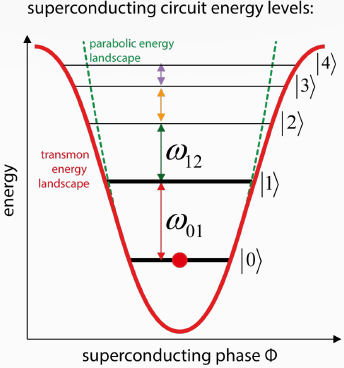
\includegraphics[width=0.4\textwidth]{immagini/transmon_potential.png}
\end{figure}
\hspace{-0.6cm}Vediamo che il potenziale ha forma approssimativamente parabolica vicino al minimo, con una piccola correzione non lineare che diventa importante per valori più grandi di $\phi$.\\
Per piccoli valori di $\phi$, il termine dominante è quindi quello quadratico, mentre il termine quartico introduce l'anarmonicità.\\
Per comprendere gli autovalori del sistema basta allora considerare cosa accadrebbe in un potenziale puramente armonico: avremmo livelli equispaziati. Qui invece, essendo il potenziale leggermente anarmonico, otteniamo livelli leggermente deformati.\\
I primi livelli presentano quindi splitting differenti:
\begin{itemize}[leftmargin=0.5cm]
    \item lo splitting tra i livelli $0$ e $1$ è $\omega_{01}$;
    \item lo splitting tra i livelli $1$ e $2$, cioè $\omega_{12}$, è più piccolo;
    \item e così via.
\end{itemize}
In queste condizioni abbiamo quindi un potenziale anarmonico e possiamo utilizzare il dispositivo come sistema a due livelli concentrandoci sui due livelli più bassi del pozzo di potenziale, che identificano gli stati computazionali $\ket*{0}$ e $\ket*{1}$.
\subsection{Driving e misura}
Abbiamo detto che ci serve un dispositivo con alcuni autolivelli, ma dobbiamo anche essere in grado di effettuare altre due operazioni fondamentali:
\begin{itemize}[leftmargin=0.5cm]
    \item il driving;
    \item la misura.
\end{itemize}
Il driving è simile a quanto fatto per il Cooper pair box: utilizziamo una tensione di gate modulata nel tempo, ad esempio tramite un drive AC periodico. Formalmente, lo descriviamo partendo dall'Hamiltoniana del sistema e aggiungendo un termine di controllo dipendente dal tempo attraverso la modulazione della tensione di gate.\\
La tensione di gate agisce sul grado di libertà di carica e, poiché il nostro obiettivo non è descrivere l'intero sistema multilivello ma solo i livelli a più bassa energia, dobbiamo effettuare una proiezione sul sottospazio bidimensionale generato dagli stati $\ket*{0}$ e $\ket*{1}$.\\
Supponiamo quindi di avere un'Hamiltoniana multilivello della forma
\begin{equation*}
    H
    =
    \sum_n E_n \ketbra*{\psi_n}{\psi_n}.
\end{equation*}
Se vogliamo limitarci ai due livelli più bassi, dobbiamo proiettare l'Hamiltoniana nel sottospazio bidimensionale generato dagli stati $\ket*{0}$ e $\ket*{1}$. Matematicamente introduciamo il proiettore
\begin{equation*}
    P
    =
    \ketbra*{0}{0}
    +
    \ketbra*{1}{1}.
\end{equation*}
La Hamiltoniana proiettata diventa quindi
\begin{equation*}
    PHP
    =
    E_0 \ketbra*{0}{0}
    +
    E_1 \ketbra*{1}{1}.
\end{equation*}
Il risultato può essere espresso anche in termini di matrici di Pauli. Includendo anche il termine di drive otteniamo
\begin{equation*}
    P(H+H_C(t))P
    =
    -\frac{\omega_{10}}{2}\sigma_z
    +
    2E_C \bar{q}_g(t) q_{01}\sigma_x
\end{equation*}
dove
\begin{equation*}
    \sigma_z
    =
    \ketbra*{1}{1}
    -
    \ketbra*{0}{0}
\end{equation*}
e
\begin{equation*}
    \sigma_x
    =
    \ketbra*{0}{1}
    +
    \ketbra*{1}{0}.
\end{equation*}
Il drive deriva dalla modulazione della tensione di gate e quindi entra attraverso l'operatore di carica $\hat{q}$. In questo caso tale operatore è non diagonale, perché gli autostati del sistema non sono più puri stati di carica: l'energia di carica non è infatti la scala energetica dominante.\\
L'idea è quindi che un drive variabile nel tempo, proporzionale a $\sigma_x$, induca transizioni tra gli stati $\ket*{0}$ e $\ket*{1}$. Questo fornisce un modo per manipolare il sistema ed effettuare operazioni sul qubit.\\
Dobbiamo ora affrontare il problema della misura.\\
Nel Cooper pair box avevamo visto una misura di tipo \emph{quantum demolition}: quando il sistema si trovava nello stato con una coppia di Cooper extra, si lasciava decadere quella coppia in quasiparticelle. In altre parole, la misura distruggeva lo stato quantistico originario.\\
Uno dei vantaggi del transmon non riguarda solo il diverso rapporto tra energia di carica ed energia Josephson, ma anche il fatto che la misura può essere effettuata in modo \emph{quantum non demolition} (QND).\\
Vediamo cosa significa. Supponiamo di avere un qubit con Hamiltoniana
\begin{equation*}
    H
    =
    \frac{\omega_{10}}{2}\sigma_z
    =
    \frac{\omega_{10}}{2}
    \qty(
        \ketbra*{1}{1}
        -
        \ketbra*{0}{0}
    ).
\end{equation*}
Effettuare una misura significa verificare, dopo l'evoluzione del sistema, se esso si trovi nello stato $\ket*{0}$ oppure nello stato $\ket*{1}$.\\
Una misura demolitrice implica che, se il sistema è inizialmente in una sovrapposizione
\begin{equation*}
    \ket*{\psi}
    =
    a\ket*{0}
    +
    b\ket*{1},
\end{equation*}
e misuriamo ad esempio lo stato $\ket*{1}$, allora dopo la misura il sistema collassa definitivamente in $\ket*{1}$: la sovrapposizione viene distrutta.\\
Una misura non demolitrice invece mira a ottenere informazione sul sistema senza distruggere la sovrapposizione.\\
Questo può essere fatto accoppiando il qubit a un dispositivo di misura. Supponiamo, ad esempio, che il dispositivo di misura sia un altro sistema a due livelli descritto da $\tau_z$. In questo caso dobbiamo considerare:
\begin{itemize}[leftmargin=0.5cm]
    \item l'Hamiltoniana del qubit;
    \item l'Hamiltoniana del dispositivo di misura;
    \item il termine di accoppiamento.
\end{itemize}
Otteniamo quindi
\begin{equation*}
    H
    =
    \frac{\omega_{10}}{2}\sigma_z
    +
    \frac{\Delta}{2}\sigma_z\tau_z
    +
    \frac{\omega_m}{2}\tau_z
\end{equation*}
dove:
\begin{itemize}[leftmargin=0.5cm]
    \item il primo termine descrive il qubit;
    \item il terzo termine descrive il meter;
    \item il secondo termine rappresenta l'accoppiamento tra i due sistemi.
\end{itemize}
L'accoppiamento è del tipo $\sigma_z\tau_z$, cioè coinvolge gli stessi operatori che compaiono nelle Hamiltoniane dei due sistemi.\mn{Questo significa che il meter ``legge'' lo stato energetico del qubit senza indurre transizioni tra $\ket*{0}$ e $\ket*{1}$, perché il termine di accoppiamento commuta con l'Hamiltoniana del qubit.}\\
Possiamo riscrivere l'Hamiltoniana nella forma
\begin{equation*}
    H
    =
    \frac{\omega_{10}}{2}\sigma_z
    +
    \frac{1}{2}
    \qty(
        \Delta\sigma_z
        +
        \omega_m
    )\tau_z.
\end{equation*}
Quello che vogliamo misurare è il meter.\\
Se il meter fosse isolato, lo splitting dei suoi livelli sarebbe semplicemente $\omega_m$. Quando però esso è accoppiato al qubit, il suo splitting diventa
\[
\omega_m \pm \Delta,
\]
a seconda dello stato del qubit:
\begin{itemize}[leftmargin=0.5cm]
    \item $\omega_m+\Delta$ se il qubit è in $\ket*{1}$;
    \item $\omega_m-\Delta$ se il qubit è in $\ket*{0}$.
\end{itemize}
Misurando quindi la frequenza del meter possiamo determinare lo stato del qubit.\\
Il punto fondamentale è che questa misura non altera lo stato del qubit, proprio perché l'accoppiamento avviene tramite $\sigma_z$, che commuta con l'Hamiltoniana del qubit. Per questo motivo la misura è di tipo quantum non demolition.\\
Vediamo ora come si realizza fisicamente questo tipo di accoppiamento:
\begin{figure}[H]
    \centering
    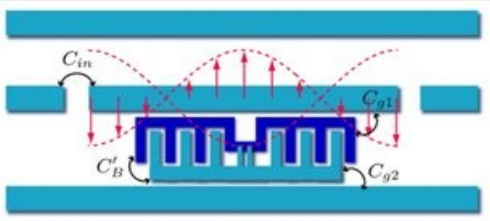
\includegraphics[width=0.5\textwidth]{immagini/Transmon_coupling.png}
\end{figure}
\hspace{-0.6cm}Osserviamo anzitutto la parte inferiore della figura. Abbiamo una regione superconduttiva blu scura, la giunzione Josephson e un secondo elettrodo azzurro chiaro. Questi due elettrodi formano la giunzione Josephson.\\
La giunzione è accoppiata a un microstrip resonator, cioè una linea conduttrice che funziona come risonatore elettromagnetico unidimensionale.\\
Poiché si tratta di un conduttore di lunghezza fissata, esso possiede modi risonanti elettromagnetici e può essere descritto circuitalmente come un circuito LC.\\
Questo risonatore è accoppiato capacitivamente al transmon tramite la capacità $C_g$.\\
Si può dimostrare che, in opportune condizioni, l'accoppiamento tra il dispositivo e il risonatore assume proprio la forma discussa in precedenza. Inoltre, anche in questo caso possiamo limitarci ai due livelli più rilevanti del sistema.\\
La figura seguente mostra il principio della misura:
\begin{figure}[H]
    \centering
    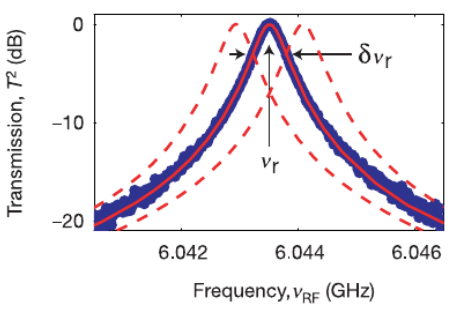
\includegraphics[width=0.7\textwidth]{immagini/Transmon_coupling_measurement.png}
\end{figure}
\hspace{-0.6cm}Quello che viene misurato è la trasmissione della linea risonante, cioè la capacità del risonatore di trasmettere segnali a una certa frequenza.\\
Se il risonatore fosse isolato, la trasmissione massima si avrebbe alla frequenza di risonanza $\omega_m$, rappresentata dalla linea continua.\\
Quando però il risonatore è accoppiato al qubit, la frequenza di risonanza si sposta di una quantità che dipende dallo stato del qubit. Le due linee tratteggiate rappresentano infatti le due possibili frequenze di risonanza del risonatore:
\begin{itemize}[leftmargin=0.5cm]
    \item una corrispondente al qubit nello stato $\ket*{0}$;
    \item l'altra corrispondente al qubit nello stato $\ket*{1}$.
\end{itemize}
Misurando quindi la trasmissione del risonatore in funzione della frequenza possiamo determinare lo stato del qubit a cui esso è accoppiato.\\
Questa misura è di tipo non demolition rispetto al qubit proprio grazie alla particolare forma dell'accoppiamento, che permette di leggere il risonatore senza alterare direttamente lo stato del qubit.
\section{Flux qubit}
Studiamo ora il flux qubit. La famiglia dei flux qubit è caratterizzata da una geometria ad anello nella quale sono presenti una o più giunzioni Josephson. In questo caso non abbiamo un elettrodo posto di fronte a una delle parti dell'anello, quindi il contributo dovuto all'energia di carica è assente oppure fortemente ridotto.\\
Il principale parametro esterno utilizzato per controllare il sistema è un campo magnetico che produce un flusso attraverso l'anello, fenomeno che sappiamo essere associato a proprietà come la quantizzazione del flusso.\\
Abbiamo già studiato l'RF-SQUID. Si tratta di uno SQUID interrotto da giunzioni Josephson e abbiamo visto che può essere utilizzato per effettuare misure estremamente sensibili di campi magnetici.\\
Se vogliamo descrivere il circuito equivalente, la struttura è molto semplice:
\begin{itemize}[leftmargin=0.5cm]
    \item abbiamo l'elemento Josephson;
    \item una geometria ad anello;
    \item un effetto capacitivo dovuto alla giunzione;
    \item e un contributo induttivo associato al loop.
\end{itemize}
Abbiamo già scritto l'equazione circuitale ottenuta dalla descrizione elettrostatica del dispositivo tramite le relazioni Josephson:
\begin{equation*}
    C \ddot{\Phi}
    +
    I_c \sin{
        \qty(
            \frac{2\pi\Phi}{\Phi_0}
        )
    }
    +
    \frac{\Phi+\Phi_x}{L}
    =
    0
\end{equation*}
dove:
\begin{itemize}[leftmargin=0.5cm]
    \item il secondo termine deriva dall'effetto Josephson;
    \item il terzo termine deriva invece dal flusso magnetico e dall'induttanza del loop.
\end{itemize}
Questi ultimi due termini definiscono il potenziale del sistema, ottenuto integrando rispetto al flusso:
\begin{equation*}
    U(\Phi)
    =
    -E_J \cos{
        \qty(
            \frac{2\pi\Phi}{\Phi_0}
        )
    }
    +
    \frac{(\Phi+\Phi_x)^2}{2L}.
\end{equation*}
Esso consiste quindi nella somma:
\begin{itemize}[leftmargin=0.5cm]
    \item dell'energia Josephson;
    \item dell'energia induttiva.
\end{itemize}
Questo potenziale svolge il ruolo di un potenziale efficace. La sua forma è relativamente semplice da comprendere:
\begin{itemize}[leftmargin=0.5cm]
    \item abbiamo un contributo parabolico in $\Phi$, con minimo in $\Phi=-\Phi_x$;
    \item a questo si sovrappone il termine coseno, che introduce una periodicità.
\end{itemize}
Il risultato è quindi un potenziale parabolico modulato periodicamente.
\begin{figure}[H]
    \centering
    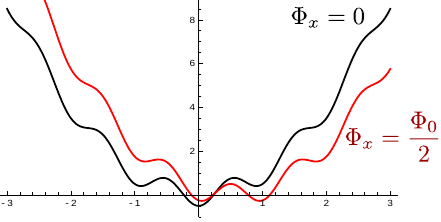
\includegraphics[width=0.6\textwidth]{immagini/flux_qubit_potential.png}
\end{figure}
\hspace{-0.6cm}La forma del potenziale dipende dal valore di $\Phi_x$, cioè dal flusso del campo magnetico esterno.\\
Ricordiamo infatti che, in una geometria ad anello, il flusso totale dipende sia dal campo magnetico applicato esternamente sia dal campo magnetico generato dalla supercorrente che circola nel loop.\\
A seconda del valore di questo flusso, il potenziale può assumere forme differenti e possedere minimi in posizioni diverse.\\
Ad esempio, se
\[
\Phi_x=0,
\]
la struttura del potenziale presenta un unico minimo in $\Phi=0$.\\
Il contributo armonico ha minimo nullo in quel punto, mentre il termine coseno fornisce il contributo $-E_J$, motivo per cui il minimo dell'energia risulta minore di zero.\\
Alla parte armonica molto dolce si sovrappone quindi il termine oscillatorio del coseno. Tuttavia, poiché il termine parabolico cresce per valori grandi di $\Phi$, l'effetto relativo delle oscillazioni del coseno diventa progressivamente meno rilevante e il potenziale appare via via più regolare.\\
Se invece
\[
\Phi_x\neq 0,
\]
i minimi del potenziale si modificano. In particolare, quando
\[
\Phi_x \approx \frac{\Phi_0}{2},
\]
il potenziale assume una forma a doppio pozzo, con due minimi distinti.\\
La forma del potenziale è all'origine della natura degli stati a più bassa energia del sistema. Prima di analizzarli, vediamo come descrivere formalmente il circuito.\\
Dobbiamo:
\begin{itemize}[leftmargin=0.5cm]
    \item scrivere l'equazione circuitale;
    \item identificare il potenziale;
    \item costruire la lagrangiana usando come variabili $\Phi$ e $\dot{\Phi}$.
\end{itemize}
La lagrangiana è
\begin{equation*}
    \mathcal{L}(\Phi,\dot{\Phi})
    =
    \frac{C}{2}\dot{\Phi}^2
    +
    E_J \cos{
        \qty(
            \frac{2\pi\Phi}{\Phi_0}
        )
    }
    -
    \frac{(\Phi+\Phi_x)^2}{2L}.
\end{equation*}
Dalla lagrangiana possiamo identificare il momento coniugato:
\begin{equation*}
    \pdv{\mathcal{L}}{\dot{\Phi}}
    =
    C\dot{\Phi}
    \equiv
    Q.
\end{equation*}
Una volta note le due variabili coniugate, possiamo scrivere l'Hamiltoniana, costituita dalla parte cinetica e da quella potenziale, e quantizzarla imponendo le relazioni di commutazione canoniche:
\begin{equation*}
    \hat{\mathcal{H}}
    =
    \frac{\hat{Q}^2}{2C}
    +
    \frac{(\hat{\Phi}+\Phi_x)^2}{2L}
    -
    E_J
    \cos{
        \biggl(
            \frac{2\pi\hat{\Phi}}{\Phi_0}
        \biggr)
    }
    \qq{,}
    \bigl[
        \hat{\Phi},
        \hat{Q}
    \bigr]
    =
    i\hbar.
\end{equation*}
Questo procedimento è esattamente analogo a quello seguito per gli altri circuiti.\\
Bisogna però ricordare una differenza fondamentale rispetto al charge qubit. Nel charge qubit la carica sulla giunzione è discreta, perché l'isola può contenere un numero intero di coppie di Cooper:
\[
0,1,2,\ldots
\]
Nel flux qubit, invece, non abbiamo un'isola isolata. Di conseguenza la carica non è discreta ma continua.\\
Questo è collegato anche al fatto che il potenziale non è periodico nella coordinata $\Phi$. Possiamo quindi imporre le usuali condizioni al contorno standard, senza necessità di imporre condizioni periodiche come nel caso del Cooper pair box.\\
Vediamo ora come viene generato il campo magnetico esterno.
\begin{figure}[H]
    \centering
    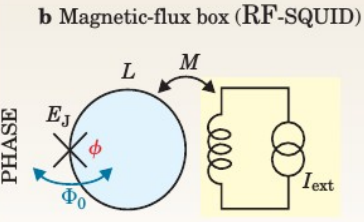
\includegraphics[width=0.5\textwidth]{immagini/flux_qubit_external_field.png}
\end{figure}
\hspace{-0.6cm}È sufficiente avere un altro circuito nelle vicinanze, percorso da corrente. Questo circuito è accoppiato induttivamente all'anello superconduttivo e produce quindi un accoppiamento magnetico tra i due sistemi.\\
Consideriamo ora l'ingrandimento del paesaggio di potenziale nel caso
\[
\Phi_x=\Phi_0.
\]
\begin{figure}[H]
    \centering
    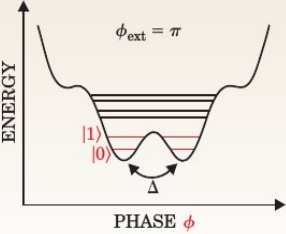
\includegraphics[width=0.5\textwidth]{immagini/flux_qubit_double_well.png}
\end{figure}
\hspace{-0.6cm}Questa figura rappresenta un ingrandimento della configurazione corrispondente alla curva rossa del grafico precedente, nella quale osserviamo chiaramente la presenza di due minimi del potenziale.\\
Qui iniziamo a passare gradualmente dall'RF-SQUID al flux qubit vero e proprio.\\
Quando il potenziale assume questa forma, gli stati a più bassa energia sono quelli rappresentati in rosso nella figura e identificano gli stati $\ket*{0}$ e $\ket*{1}$.\\
Dalla meccanica quantistica sappiamo che:
\begin{itemize}[leftmargin=0.5cm]
    \item se la barriera tra i due pozzi è molto alta, il sistema si comporta quasi classicamente e gli stati fondamentali risultano localizzati nel pozzo sinistro o destro;
    \item se invece la barriera si abbassa, compare il tunneling quantistico tra i due minimi.
\end{itemize}
In questo secondo caso, gli autostati diventano sovrapposizioni degli stati localizzati:
\begin{equation*}
    \ket*{0}
    =
    \frac{1}{\sqrt{2}}
    \qty(
        \ket*{L}
        +
        \ket*{R}
    )
    \qq{,}
    \ket*{1}
    =
    \frac{1}{\sqrt{2}}
    \qty(
        \ket*{L}
        -
        \ket*{R}
    )
\end{equation*}
Questi sono quindi:
\begin{itemize}[leftmargin=0.5cm]
    \item lo stato simmetrico;
    \item lo stato antisimmetrico;
\end{itemize}
rispetto allo scambio tra i due pozzi.\\
In questo caso gli stati $\ket*{0}$ e $\ket*{1}$ sono quindi sovrapposizioni di stati localizzati nei due minimi del potenziale.\\
Come nei casi precedenti, possiamo troncare lo spazio di Hilbert ai due livelli più bassi, assumendo che gli altri siano sufficientemente separati energeticamente.\\
Otteniamo nuovamente un sistema efficace a due livelli descritto tramite matrici di Pauli:
\begin{equation*}
    \hat{\mathcal{H}}
    \to
    \hat{\mathcal{H}}_Q
    =
    -\frac{\epsilon(\Phi_x)}{2}\sigma_z
    -
    \frac{\Delta(E_J)}{2}\sigma_x.
\end{equation*}
I parametri di controllo esterni sono:
\begin{itemize}[leftmargin=0.5cm]
    \item il campo magnetico, cioè il flusso $\Phi_x$;
    \item in linea di principio anche l'energia Josephson $E_J$, che può essere resa controllabile.
\end{itemize}
Vediamo come questo possa essere realizzato:
\begin{figure}[H]
    \centering
    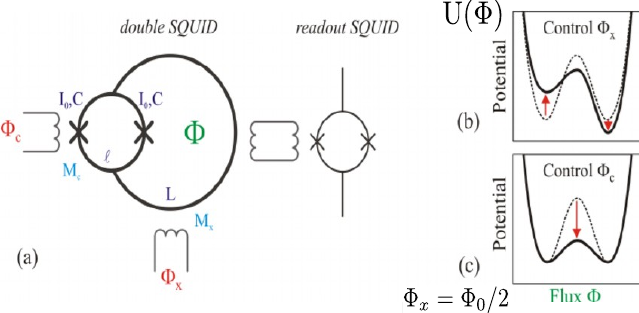
\includegraphics[width=0.8\textwidth]{immagini/flux_qubit_modulation_E_J.png}
\end{figure}
\hspace{-0.6cm}Invece di utilizzare una singola giunzione Josephson, possiamo sostituirla con un piccolo loop contenente due giunzioni Josephson.\\
Questo nuovo elemento si comporta ancora come un elemento Josephson efficace, ma con un'energia Josephson dipendente dal flusso magnetico che attraversa il piccolo loop.\\
In questo modo otteniamo una Josephson energy modulabile.\\
In configurazioni di questo tipo abbiamo quindi due controlli distinti:
\begin{itemize}[leftmargin=0.5cm]
    \item $\Phi_x$, generato dal circuito che produce il flusso principalmente nel loop grande;
    \item $\Phi_c$, prodotto da un secondo circuito accoppiato principalmente al loop piccolo.
\end{itemize}
Possiamo quindi:
\begin{itemize}[leftmargin=0.5cm]
    \item modificare $\Phi_x$;
    \item oppure modulare efficacemente $E_J$ tramite $\Phi_c$.
\end{itemize}
In queste configurazioni i due parametri di controllo permettono quindi di modificare la forma del potenziale oppure, facendoli variare nel tempo, di eseguire operazioni sugli stati del qubit.\\
Ad esempio, variando il bias $\Phi_c$ possiamo modificare l'altezza della barriera del doppio pozzo. In pratica il potenziale può passare:
\begin{itemize}[leftmargin=0.5cm]
    \item da una configurazione a doppio pozzo;
    \item a un potenziale quasi quartico;
    \item fino a una forma quasi armonica;
    \item oppure tornare a un doppio pozzo asimmetrico.
\end{itemize}
Queste modifiche possono essere realizzate sperimentalmente.\\
I due controlli agiscono in modo differente:
\begin{itemize}[leftmargin=0.5cm]
    \item $\Phi_x$ modifica principalmente la simmetria del potenziale;
    \item $\Phi_c$ controlla principalmente l'altezza della barriera.
\end{itemize}
\subsection{Driving e misura}
Abbiamo detto che ci servono due livelli ben definiti e la possibilità di pilotarli. Questo può essere fatto, ad esempio, tramite il flusso magnetico esterno. Inoltre, dobbiamo essere in grado di effettuare la misura del sistema.\\
Gli ingredienti fondamentali sono quindi sempre gli stessi: driving e misura.\\
Per effettuare la misura sfruttiamo il fatto che i due stati del flux qubit corrispondono a differenti correnti che circolano nel circuito.\\
Possiamo quindi accoppiare questo circuito a un secondo loop superconduttivo e misurare il flusso magnetico attraverso tale loop, che dipenderà dallo stato del qubit.\\
Anche in questo caso si tratta quindi di una misura di tipo non demolition. L'accoppiamento con il secondo circuito avviene tramite un'induttanza mutua.\\
Vediamo un possibile circuito realizzato sperimentalmente:
\begin{figure}[H]
    \centering
    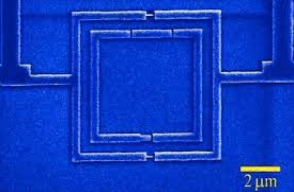
\includegraphics[width=0.5\textwidth]{immagini/flux_qubit_circuit.png}
\end{figure}
\hspace{-0.6cm}La parte interna rappresenta l'anello superconduttivo che realizza il flux qubit, mentre l'anello più grande esterno costituisce il circuito di misura.\\
Quest'ultimo contiene due giunzioni Josephson e viene utilizzato per misurare il flusso magnetico generato dall'anello interno.\\
In pratica, ciò che si misura è il flusso attraverso il loop più grande, che dipende dal flusso magnetico prodotto dalla corrente che circola nell'anello interno.\\
Misurando quindi il flusso — oppure equivalentemente la corrente che circola nel loop esterno — possiamo determinare lo stato dell'anello interno, che, se correttamente polarizzato, può trovarsi soltanto in due stati distinti.
\section{Tempo di vita dei qubit}
Consideriamo ora l'evoluzione di questi qubit nel corso degli anni.
\begin{figure}[H]
    \centering
    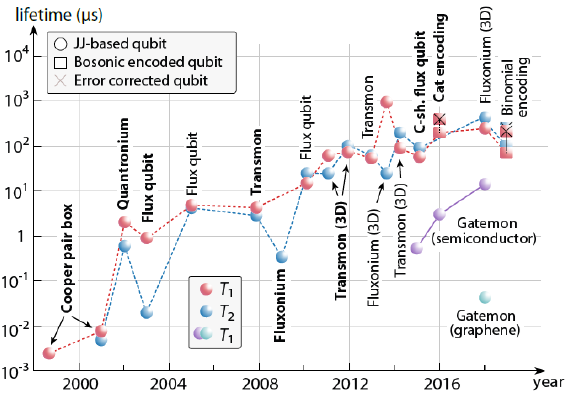
\includegraphics[width=0.7\textwidth]{immagini/qubit_lifetime.png}
\end{figure}
\hspace{-0.6cm}Qui vediamo il cosiddetto tempo di vita del qubit (\emph{qubit lifetime}) in funzione dell'anno in cui il dispositivo è stato realizzato.\\
Il tempo di vita del qubit è una misura di quanto rapidamente decadano nel tempo le oscillazioni coerenti del sistema. Abbiamo infatti visto, nel caso del charge qubit e del flux qubit, che le oscillazioni che descrivono il passaggio coerente del qubit tra i due stati non persistono indefinitamente: invece di oscillare periodicamente per sempre, esse decadono nel tempo secondo una certa legge di decadimento, spesso di tipo esponenziale, caratterizzata da una scala temporale chiamata $T_1$.\\
Nel grafico è riportato proprio questo tempo di vita $T_1$ per differenti tipi di qubit.\\
Vediamo innanzitutto il Cooper pair box, cioè il primo dispositivo che abbiamo discusso, con tempi di coerenza dell'ordine dei nanosecondi, addirittura inferiori a $10\,\mathrm{ns}$.\\
Successivamente, passando al quantronium e poi al transmon, osserviamo un aumento del tempo di rilassamento di circa tre o quattro ordini di grandezza. Analogamente, anche altre tipologie di qubit mostrano un miglioramento progressivo nel tempo.\\
Questo incremento del tempo di coerenza è il risultato di differenti sforzi sperimentali, riconducibili principalmente a due strategie:
\begin{itemize}[leftmargin=0.5cm]
    \item ridurre le sorgenti di rumore;
    \item ottimizzare il dispositivo e il suo controllo.
\end{itemize}
Ridurre il rumore significa innanzitutto utilizzare materiali migliori, dove ``migliori'' significa soprattutto materiali con un numero minore di difetti.\\
Inoltre, si possono utilizzare configurazioni circuitali migliori, cioè progettare il dispositivo in modo da renderlo meno sensibile alle sorgenti di rumore. Un esempio importante di questa strategia è proprio il transmon.\\
Questa è quindi una prima linea di intervento.\\
La seconda consiste invece nell'ottimizzazione dinamica del dispositivo, ad esempio tramite controlli dipendenti dal tempo come tensioni o flussi magnetici. In pratica, si utilizzano segnali di controllo opportunamente progettati per ridurre l'effetto delle sorgenti di rumore.\\
Questa ottimizzazione può essere realizzata con approcci differenti, anche numerici, utilizzando tecniche di intelligenza artificiale o machine learning.\\
Tutto questo serve a sottolineare che questi circuiti, chiamati spesso atomi artificiali superconduttivi, sono fortemente influenzati da sorgenti di rumore che derivano dai materiali microscopici utilizzati per realizzare il circuito stesso.\\
Pensiamo, ad esempio, al Cooper pair box. La giunzione tunnel e gli elettrodi superconduttivi sono tipicamente depositati sopra un substrato dielettrico. In questi materiali — sia nello strato isolante sia nel substrato — possono essere presenti impurità e difetti strutturali.\\
Abbiamo infatti detto che una giunzione Josephson, nella sua implementazione più semplice, è ottenuta depositando due strati superconduttivi separati da un ossido sottile. Questo ossido costituisce la barriera attraverso la quale avviene l'effetto Josephson.\\
Sia nell'ossido sia nel substrato possono quindi essere naturalmente presenti difetti. Alcuni di questi difetti possono essere carichi elettricamente.\\
Possiamo pensare, ad esempio, a una giunzione Josephson in alluminio:
\begin{itemize}[leftmargin=0.5cm]
    \item abbiamo gli elettrodi di alluminio;
    \item tra essi è presente uno strato di ossido di alluminio;
    \item idealmente l'ossido dovrebbe essere un cristallo regolare;
    \item tuttavia possono comparire difetti configurazionali.
\end{itemize}
Questi difetti possono essere schematizzati come minimi addizionali del potenziale all'interno dello strato isolante. Una carica può allora localizzarsi in uno oppure nell'altro di questi minimi.\\
A seconda della posizione occupata dalla carica, cambia la polarizzazione dell'isola superconduttiva.\\
Questo accade perché il dispositivo è estremamente piccolo, tipicamente dell'ordine di pochi nanometri, e quindi anche una singola carica può influenzare significativamente il potenziale elettrostatico dell'isola.\\
Queste impurità, chiamate \emph{background charges}, possono fluttuare nel tempo:
\begin{itemize}[leftmargin=0.5cm]
    \item la carica può trovarsi in una configurazione;
    \item poi passare all'altra;
    \item e così via.
\end{itemize}
In questo modo esse inducono una polarizzazione fluttuante dell'isola superconduttiva.\\
In pratica non è presente un singolo difetto ma un gran numero di difetti, che producono un rumore nella polarizzazione dell'isola con spettro caratteristico di tipo $\frac{1}{f}$, cioè un rumore che cresce fortemente alle basse frequenze.\\
Questa è una delle principali sorgenti di rumore negli atomi artificiali superconduttivi e, in particolare nel charge qubit, è responsabile del rapido decadimento delle oscillazioni coerenti.\\
Nella prima generazione di qubit superconduttivi questo tipo di rumore era estremamente dannoso ed era la principale limitazione sperimentale.\\
Il miglioramento dei charge qubit è quindi dovuto sia:
\begin{itemize}[leftmargin=0.5cm]
    \item all'ottimizzazione del design del dispositivo;
    \item sia all'utilizzo di materiali migliori.
\end{itemize}
Queste sono proprio le due strategie che abbiamo discusso prima:
\begin{itemize}[leftmargin=0.5cm]
    \item riduzione del rumore tramite materiali migliori;
    \item ottimizzazione del dispositivo tramite progettazione circuitale e tecniche di controllo.
\end{itemize}
Questo tipo di rumore a spettro $1/f$ è tipico delle implementazioni basate sulla carica, ma è presente anche nei flux qubit e nei phase qubit.\\
Consideriamo ora due difetti carichi. Essi costituiscono essenzialmente un dipolo elettrico, che può oscillare nel tempo.\\
Abbiamo già detto che, nei dispositivi con isola superconduttiva, l'oscillazione bistabile di una singola carica all'interno della giunzione può produrre una polarizzazione fluttuante dell'isola. Questa è precisamente l'origine del rumore di carica associato alle fluttuazioni della polarizzazione.\\
Processi di questo tipo possono influenzare anche la corrente critica della giunzione.\\
Ricordiamo infatti che la corrente critica è la massima supercorrente che la giunzione può sostenere e dipende dalle proprietà microscopiche della giunzione stessa.\\
Se all'interno del materiale che costituisce la giunzione sono presenti dipoli fluttuanti, possiamo pensare che tali fluttuazioni modifichino localmente la trasparenza della giunzione, e quindi il valore massimo di supercorrente sostenibile.\\
Le fluttuazioni dei dipoli inducono quindi anche fluttuazioni della corrente critica.\\
Tali fluttuazioni sono state osservate sperimentalmente e mostrano anch'esse uno spettro con forti componenti a bassa frequenza.\\
Tutto questo serve a dire che tutte le implementazioni menzionate — charge, flux e phase qubit — soffrono di rumore con spettro $1/f$, generato da differenti meccanismi microscopici:
\begin{itemize}[leftmargin=0.5cm]
    \item alcuni relativamente ben compresi;
    \item altri ancora oggetto di studio teorico e sperimentale.
\end{itemize}
Processi di questo tipo sono presenti anche in giunzioni Josephson basate su grafene:
\begin{figure}[H]
    \centering
    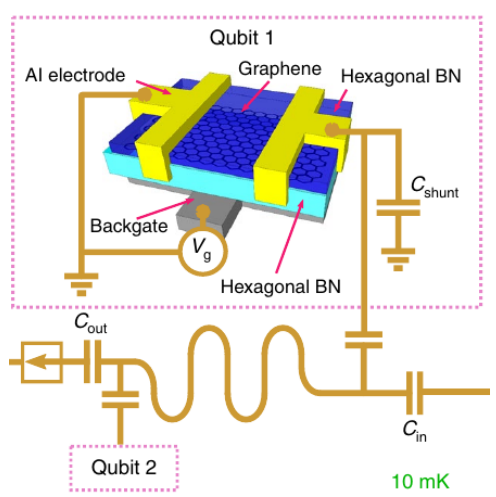
\includegraphics[width=0.5\textwidth]{immagini/graphene_junction.png}
\end{figure}
\hspace{-0.6cm}In questo caso abbiamo uno strato di grafene posto tra due strati di nitruro di boro esagonale, che lo isolano molto bene, mentre i contatti superconduttivi sono realizzati lateralmente quasi in geometria unidimensionale.\\
Quando questa giunzione viene inserita in un circuito, può essere controllata tramite una tensione di gate e il dispositivo viene chiamato \emph{gatemon}, poiché è molto simile al transmon, con la differenza principale che la giunzione Josephson tradizionale è sostituita da una giunzione Josephson a grafene.\\
Anche in questo caso il sistema è sensibile a diverse sorgenti di fluttuazione, ad esempio fluttuazioni della densità di portatori nel grafene.\\
Infatti il grafene possiede una certa densità elettronica che può fluttuare nel tempo e, quando questo elemento viene utilizzato all'interno della giunzione Josephson, tali fluttuazioni introducono rumore nel circuito.\\
Questo tipo di rumore è simile a quello presente nei dispositivi CMOS a semiconduttore.\\
In generale, quando sono presenti ossidi, esistono impurità e trappole di carica. Nei dispositivi CMOS, ad esempio, la corrente dovrebbe fluire dal source al drain, ma se esistono trappole di carica nell'ossido alcune cariche possono venire intrappolate invece di attraversare il canale.\\
Questo processo produce rumore nella corrente.\\
Se esiste un gran numero di trappole distribuite casualmente nello strato isolante, la combinazione dei processi di intrappolamento produce un rumore con spettro $\frac{1}{f}$.\\
Si tratta quindi di un fenomeno estremamente generale nei dispositivi a stato solido:
\begin{itemize}[leftmargin=0.5cm]
    \item transistor a semiconduttore;
    \item circuiti superconduttivi;
    \item dispositivi per tecnologie quantistiche;
    \item altri sistemi artificiali nanostrutturati.
\end{itemize}

% \chapter*{Appendice A}
% \addcontentsline{toc}{chapter}{Appendice A}
% \input{appendici/AppendiceA}

% Bibliografia
% \makeatletter
% \let\ps@plain\ps@fancytitle\makeatother
\cleardoublepage\phantomsection
\backmatter\printbibheading[heading=bibintoc]
%\vspace{5mm}


\printbibliography[type=book,heading=subbibliography,title={Libri di testo}]

\selectlanguage{english}
\printbibliography[nottype=book,heading=subbibliography,title={Altri riferimenti}]



%\newgeometry{margin=0.5in}


% Indice analitico
%\addcontentsline{toc}{part}{}{}   %%% Fix al link all'indice analitico. Funziona solo se titleformat part è vuoto.
% \fancyhead[RO]{\makebox[0pt][l]{\makebox[\myoddoffset][r]{\thepage}}}
% \fancyhead[LE]{\makebox[0pt][r]{\makebox[\myoddoffset][l]{\thepage}}}
% \newgeometry{
%   left = 2.3cm,
%   right=1cm,
%   marginparsep=0cm,
%   marginparwidth=0cm,
%   top=2.3cm,bottom=2.3cm,
% }
\newgeometry{
    top=2.3cm,bottom=2.3cm,
    %% Margini
    left = 2.3cm,
    right=3.2cm,
    marginparsep=0cm,
    marginparwidth=2.3cm,
    %%% Contenuto
    %textwidth=14cm,
    %textheight=180mm,
    %headheight=21pt,
    %%%%%%5 Header e footer
    %headsep=10pt,
    %footskip=20pt,
    %footnotesep=10pt,
}
\scriptsize
\renewcommand{\indexname}{Indice analitico}
% CHANGE PLAIN STYLE
% \makeatletter
% \let\ps@plain\ps@fancytitle\makeatother
%\thispagestyle{fancytitle}
\cleardoublepage\phantomsection
\printindex
\end{document}